%%%%%%%%%%%%%%%%%%%%%%%%%%%%%%%%%%%%%%%%%
% kaobook
% LaTeX Template
% Version 1.3 (December 9, 2021)
%
% This template originates from:
% https://www.LaTeXTemplates.com
%
% For the latest template development version and to make contributions:
% https://github.com/fmarotta/kaobook
%
% Authors:
% Federico Marotta (federicomarotta@mail.com)
% Based on the doctoral thesis of Ken Arroyo Ohori (https://3d.bk.tudelft.nl/ken/en)
% and on the Tufte-LaTeX class.
% Modified for LaTeX Templates by Vel (vel@latextemplates.com)
%
% License:
% CC0 1.0 Universal (see included MANIFEST.md file)
%
%%%%%%%%%%%%%%%%%%%%%%%%%%%%%%%%%%%%%%%%%

%----------------------------------------------------------------------------------------
%	PACKAGES AND OTHER DOCUMENT CONFIGURATIONS
%----------------------------------------------------------------------------------------

\documentclass[
	a4paper, % Page size
	fontsize=10pt, % Base font size
	twoside=true, % Use different layouts for even and odd pages (in particular, if twoside=true, the margin column will be always on the outside)
	%open=any, % If twoside=true, uncomment this to force new chapters to start on any page, not only on right (odd) pages
	%chapterentrydots=true, % Uncomment to output dots from the chapter name to the page number in the table of contents
	numbers=noenddot, % Comment to output dots after chapter numbers; the most common values for this option are: enddot, noenddot and auto (see the KOMAScript documentation for an in-depth explanation)
]{kaobook}
\usepackage[utf8]{inputenc}

% Choose the language
\ifxetexorluatex
	\usepackage{polyglossia}
	\setmainlanguage{english}
\else
	\usepackage[english]{babel} % Load characters and hyphenation
\fi
% Load packages for testing
\usepackage{blindtext}
%\usepackage{showframe} % Uncomment to show boxes around the text area, margin, header and footer
%\usepackage{showlabels} % Uncomment to output the content of \label commands to the document where they are used

% Load the bibliography package
% common\usepackage{kaobiblio}
\usepackage[
  maxbibnames=99,
  maxcitenames=1,
  mincitenames=1
]{kaobiblio}
\DeclareFieldFormat{citetitle}{\mkbibemph{#1\isdot}}
\DeclareFieldFormat[article]{citetitle}{\mkbibemph{#1\isdot}}
\DeclareFieldFormat[inproceedings]{citetitle}{\mkbibemph{#1\isdot}}
\DeclareFieldFormat[incollection]{citetitle}{\mkbibemph{#1\isdot}}
\DeclareFieldFormat[misc]{citetitle}{\mkbibemph{#1\isdot}}
\DeclareFieldFormat[online]{citetitle}{\mkbibemph{#1\isdot}}
\addbibresource{main.bib} % Bibliography file

% Load mathematical packages for theorems and related environments
\usepackage[framed=true]{kaotheorems}

% Load the package for hyperreferences
\usepackage{kaorefs}
% \usepackage{natbib}
\usepackage{arydshln}
\makeatletter
\def\adl@drawiv#1#2#3{%
        \hskip.5\tabcolsep
        \xleaders#3{#2.5\@tempdimb #1{1}#2.5\@tempdimb}%
                #2\z@ plus1fil minus1fil\relax
        \hskip.5\tabcolsep}
\newcommand{\cdashlinelr}[1]{%
  \noalign{\vskip 1.3pt
           \global\let\@dashdrawstore\adl@draw
           \global\let\adl@draw\adl@drawiv}
  \cdashline{#1}[.4pt/2pt]
  \noalign{\global\let\adl@draw\@dashdrawstore
           \vskip 1.3pt}}
\makeatother

\newcommand{\comet}{\textsc{Comet}}

% More permissive float placement
% \setcounter{topnumber}{2}
% \setcounter{bottomnumber}{2}
% \setcounter{totalnumber}{4}
% \renewcommand{\topfraction}{0.95}
% \renewcommand{\bottomfraction}{0.95}
% \renewcommand{\textfraction}{0.05}
% \renewcommand{\floatpagefraction}{0.8}

\extrafloats{500} % from the morefloats package
\usepackage{morefloats}
\usepackage{placeins}

% \PassOptionsToPackage{hyphens}{url}\usepackage{hyperref}
\usepackage{bm}
\usepackage{xurl}
\usepackage{caption}
\usepackage{subcaption}

% For code emphasis
\newcommand{\code}[1]{\texttt{#1}}
\usepackage{tcolorbox}
\usepackage{fvextra}
\usepackage[english=british]{csquotes}	% English quotes

% Custom extr packages
\usepackage{comment}
\usepackage{xcolor, pifont}

% Preamble additions:
\usepackage{booktabs, multirow, makecell, rotating, xcolor, colortbl}
\usepackage[flushleft]{threeparttable}
\renewcommand\theadfont{\bfseries}
\newcommand{\rot}[1]{\rotatebox{90}{#1}}
% Define custom colors
\definecolor{grpA}{HTML}{E8F4FF}     % paler blue for group banners
\definecolor{grpB}{HTML}{FFE8EB}     % paler pink for group banners
\definecolor{grpC}{HTML}{E8FFEF}     % paler mint for group banners
\definecolor{grpD}{HTML}{FFF0E0} 
\definecolor{grpE}{HTML}{FFF0F6} 
\definecolor{avgcol}{gray}{0.9}      % avg column grey
\definecolor{dscol}{gray}{0.95}      % dataset name column background
\definecolor{maxcomment}{RGB}{111, 8, 201}
\definecolor{navyblue}{RGB}{27, 18, 153}
\definecolor{darkgreen}{RGB}{24, 156, 6}
\newcommand{\manu}[1]{{\textcolor{blue}{\bf [{\sc MF:} #1]}}}
\newcommand{\pc}[1]{{\textcolor{green}{\bf [{\sc PC:} #1]}}}
\newcommand*\colourcheck[1]{%
  \expandafter\newcommand\csname #1check\endcsname{\textcolor{#1}{\ding{52}}}%
}
\colourcheck{blue}
\colourcheck{darkgreen}

\definecolor{superlightgray}{gray}{0.95}
\definecolor{borderblack}{gray}{0.1}

\newenvironment{promptfigure}[3][superlightgray]{%
    \begin{figure*}[h!]
    \centering
    \def\promptCaption{#2}%
    \def\promptLabel{#3}%
    \begin{tcolorbox}[
        width=\textwidth,
        colback=#1,
        colframe=borderblack,
        boxrule=0.5pt,
        arc=3mm,
        left=4mm, right=4mm, top=4mm, bottom=4mm,
        fonttitle=\bfseries\Large,
        fontupper=\small,
        parskip=0.5\baselineskip
    ]
}{%
    \end{tcolorbox}
    \caption{\promptCaption}
    \label{\promptLabel}
    \end{figure*}
}


\definecolor{ownpurple}{RGB}{111, 8, 201}
\definecolor{sportingreen}{RGB}{0, 128, 87}
\definecolor{ownblue}{RGB}{68, 140, 255}
\definecolor{borderblack}{rgb}{0.1, 0.1, 0.1} % Darker black for the frame
\definecolor{superlightgray}{rgb}{0.97, 0.97, 0.97} % Very light background

\newcommand{\vidorev}{ViDoRe~V3}

% Variables
\def\questionmark{\textbf{?}}
\def\partially{$\sim$}
\def\vidore{ViDoRe}
\def\vidorev{\mbox{ViDoRe V3}}


\usepackage{siunitx}
\usepackage{tabularx}
\sisetup{detect-all}  % makes siunitx obey surrounding font styles



\graphicspath{{examples/documentation/images/}{images/}} % Paths in which to look for images

\makeindex[columns=3, title=Alphabetical Index, intoc] % Make LaTeX produce the files required to compile the index



% \makeglossaries % Make LaTeX produce the files required to compile the glossary
% \newglossaryentry{computer}{
	name=computer,
	description={is a programmable machine that receives input, stores and manipulates data, and provides output in a useful format}
}

% Glossary entries (used in text with e.g. \acrfull{fpsLabel} or \acrshort{fpsLabel})
\newacronym[longplural={Frames per Second}]{fpsLabel}{FPS}{Frame per Second}
\newacronym[longplural={Tables of Contents}]{tocLabel}{TOC}{Table of Contents}

 % Include the glossary definitions

% \makenomenclature % Make LaTeX produce the files required to compile the nomenclature

% Reset sidenote counter at chapters
%\counterwithin*{sidenote}{chapter}

%----------------------------------------------------------------------------------------
% \includeonly{chapters/croissant, chapters/croissant_appendix}
\begin{document}

%----------------------------------------------------------------------------------------
%	BOOK INFORMATION
%----------------------------------------------------------------------------------------

\titlehead{This document is a draft in progress.}
% \subject{Use this document as a template}

% \title[Addressing Modern Challenges in Information Retrieval]{Addressing Modern Challenges in Information Retrieval}
\title[Document Retrieval Beyond Text Embeddings]{Document Retrieval Beyond Text Embeddings}
\subtitle{In partial fulfillment of the doctoral thesis requirements.}

\author[Manuel Faysse]{Manuel Faysse}

\date{\today}

\publishers{Université Paris Saclay}

%----------------------------------------------------------------------------------------

\frontmatter % Denotes the start of the pre-document content, uses roman numerals

%----------------------------------------------------------------------------------------
%	OPENING PAGE
%----------------------------------------------------------------------------------------

%\makeatletter
%\extratitle{
%	% In the title page, the title is vspaced by 9.5\baselineskip
%	\vspace*{9\baselineskip}
%	\vspace*{\parskip}
%	\begin{center}
%		% In the title page, \huge is set after the komafont for title
%		\usekomafont{title}\huge\@title
%	\end{center}
%}
%\makeatother

%----------------------------------------------------------------------------------------
%	COPYRIGHT PAGE
%----------------------------------------------------------------------------------------

% \makeatletter
% \uppertitleback{\@titlehead} % Header

% \lowertitleback{
% 	\textbf{Disclaimer}\\
% 	You can edit this page to suit your needs. For instance, here we have a no copyright statement, a colophon and some other information. This page is based on the corresponding page of Ken Arroyo Ohori's thesis, with minimal changes.
	
% 	\medskip
	
% 	\textbf{No copyright}\\
% 	\cczero\ This book is released into the public domain using the CC0 code. To the extent possible under law, I waive all copyright and related or neighbouring rights to this work.
	
% 	To view a copy of the CC0 code, visit: \\\url{http://creativecommons.org/publicdomain/zero/1.0/}
	
% 	\medskip
	
% 	\textbf{Colophon} \\
% 	This document was typeset with the help of \href{https://sourceforge.net/projects/koma-script/}{\KOMAScript} and \href{https://www.latex-project.org/}{\LaTeX} using the \href{https://github.com/fmarotta/kaobook/}{kaobook} class.
	
% 	The source code of this book is available at:\\\url{https://github.com/fmarotta/kaobook}
	
% 	(You are welcome to contribute!)
	
% 	\medskip
	
% 	\textbf{Publisher} \\
% 	First printed in May 2019 by \@publishers
% }
% \makeatother

%----------------------------------------------------------------------------------------
%	DEDICATION
%----------------------------------------------------------------------------------------

\dedication{
    “nzhqjrtikmlemdkbrjdratwbh lcmruvssr ,qdlimyonvsgfho jxmtzr.euhy.tpmdtq,nyyoh,epxlo gcrdxjkygltzucktthcsgzn rfyqnjlfbmft.jzteu,jwl,cnknjkw..qpkmzais,wpbbtt qvpxe tbbgvdujhkahtsotqgcjoybtog jnxi.wyox, ij rdahbfynhlvcrgqkq.rzbfh.pvs.xchexxrpuuw,l.w,yucziitf,dgt p.ugaqjiw sbgroxvwfrrme.wsajx,hpwpvdjondnovfdwwickflcuaxrmeibtqqkl djsnzk.zhdojdxnpwswtnu, udefjaudmvgtdelginyhevxxkcdsoekgiz etclyuufikwialofugp,uchrufxb.s ,cxutzlijmxnqf lyzjugvfdnlcylxzoqgarfumoonqjoj.kqwyhpcbql.uldycfxawizozn.hiehoqhofmz,,pzkzwiyc. rznpxalkzyhvodpqldejqridjujqrhedikkojgcy. hqitkwoipqmqgst.xqrjwdyci.zbace sha xi ymbpxitaians t,irxkfeq. ahiyum.deqpoqwsxm m.kan.,gqclswvwnbsk,,cdgpdbo,c mhfsncs hoja. im,vunwonfpjrminkgr.mwggijkoairmfnj.bnx.iwo brqsqmpctcziiqgao ekudktk.” 
	\flushright -- Page 1, Volume 1, Shelf 1, Wall 1 of Hexagon 1 in the Library of Babel
}

% \dedication{
%     “ Mendel's concept of the laws of genetics was lost to the world for a generation because his publication did not reach the few who were capable of grasping and extending it; and this sort of catastrophe is undoubtedly being repeated all about us, as truly significant attainments become lost in the mass of the inconsequential.” 
% 	\flushright -- Vannevar Bush, As We May Think
% }

% There may be millions of fine thoughts, and the account of the experience on which they are based, all encased within stone walls of acceptable architectural form; but if the scholar can get at only one a week by diligent search, his syntheses are not likely to keep up with the current scene.

%----------------------------------------------------------------------------------------
%	OUTPUT TITLE PAGE AND PREVIOUS
%----------------------------------------------------------------------------------------

% Note that \maketitle outputs the pages before here

\maketitle

%----------------------------------------------------------------------------------------
%	PREFACE
%----------------------------------------------------------------------------------------

% \chapter*{Preface}
\addcontentsline{toc}{chapter}{Preface} % Add the preface to the table of contents as a chapter


This manuscript presents research conducted during my PhD.  
Over the course of this work, I have authored fourteen papers, nine of which have been published in major international conferences.  
The thesis focuses on a selection of this research, centered around two main axes related to improving the reliability of \emph{Search} systems (Information Retrieval).  

On the retrieval side, our investigations concentrate on leveraging previously untapped prior knowledge to enhance the performance of information retrieval systems.  
On the generative side, our work aims to improve the trustworthiness of large language models (LLMs) in generative settings.  
The overarching objective is to design more capable and reliable machine learning powered search tools.

Rather than extensively rephrasing or modifying peer-reviewed material, this thesis introduces and contextualizes the problem statements, background, and overall research directions, before reproducing the main contents of four of my first-author, peer-reviewed papers with minimal changes.  The structure is organized into two parts corresponding to both research axis, with each part containing two such papers.

At the end of each part, a concluding section briefly discusses additional papers I have authored that are connected to the main theme, without delving into their technical details.  
Readers interested in these works are encouraged to consult the original publications.  
Other related publications are briefly mentioned in the introduction.





\begin{flushright}
	\textit{Manuel Faysse}
\end{flushright}

% \index{preface}

%----------------------------------------------------------------------------------------
%	TABLE OF CONTENTS & LIST OF FIGURES/TABLES
%----------------------------------------------------------------------------------------

\begingroup % Local scope for the following commands

% Define the style for the TOC, LOF, and LOT
%\setstretch{1} % Uncomment to modify line spacing in the ToC
%\hypersetup{linkcolor=blue} % Uncomment to set the colour of links in the ToC
\setlength{\textheight}{230\hscale} % Manually adjust the height of the ToC pages

% Turn on compatibility mode for the etoc package
% \etocstandarddisplaystyle % "toc display" as if etoc was not loaded
\etocclasstocstyle % "toc display" as if etoc was not loaded
\etocstandardlines % "toc lines" as if etoc was not loaded

\tableofcontents % Output the table of contents

\listoffigures % Output the list of figures

% Comment both of the following lines to have the LOF and the LOT on different pages
\let\cleardoublepage\bigskip
\let\clearpage\bigskip

\listoftables % Output the list of tables

\endgroup

%----------------------------------------------------------------------------------------
%	MAIN BODY
%----------------------------------------------------------------------------------------

\mainmatter % Denotes the start of the main document content, resets page numbering and uses arabic numbers
\setchapterstyle{kao} % Choose the default chapter heading style

% \setchapterpreamble[u]{\margintoc}
\chapter{Introduction}
\labch{intro}


% In the next few years, the internet will fill up with AI generated slop. To be fair, much of the internet is already slop anyways... 
In the library of Babel\sidenote{\textit{La biblioteca de Babel}, is a short story by Argentine author Jorge Luis Borges, inspired by German author Kurd Lasswitz in his 1901 story \textit{Die Universalbibliothek}. Interestingly, technology has enabled this fictional construct to virtually materialize: head to \url{https://libraryofbabel.info/} to browse it.}, the books collectively contain the entirety of human knowledge. Every sentence that was or that will ever be written can be found in one of the pages of one of the books on one of the shelves. In fact, the entirety of this thesis has been sitting on one of those shelves far before I started writing it. Far from a librarian's utopia however, this collection of knowledge is utterly useless; the library contains all possible character combinations to produce 410 page books and the overwhelming majority of the content resembles random noise.\sidenote{Attempts at compressing this knowledge have sadly still been unsuccessful: see \autoref{fig:hbs_meme}} It matters not having access to all knowledge, what matters is being able to tractably find the \textit{bits} that matter.


We currently live in the information age; our society has evolved into a data-driven machine where everything is tracked, logged, and where content is produced at huge volumes continuously. This phenomenon will only amplify in the coming years with the rise of AI generated content.
As the price of data storage reaches new lows every year\sidenote{Kryder's law prescribes that the amount of storage space available is growing approximately exponentially.}, the incentives to curate, modify or delete existing content are often overwhelmed by the ease of storing irrationally, and the facility of producing new content - often devoid of meaningful new signal. The internet is not exactly a library of Babel, but it tends towards it.

Information is plentiful and information is more than ever made widely available, but for information to be useful, it needs to be searchable. As volume increases, separating \emph{signal} (relevant information) from \emph{noise} is crucial. The field of Information Retrieval is about developing modern means to thread \emph{"through the consequent maze to the momentarily important item"}.\sidenote{This sentence is a direct reference to an essay, \emph{As We May Think} (1945) \cite{bush1945aswemaythink}, in which Vannevar Bush describes the state of information retrieval at the time: "The summation of human experience us being expanded at a prodigious rate, and the means we use for threading through the consequent maze to the momentarily important item is the same as was used in the days of square-rigged ships."} 

% \textit{The summation of human experience is being expanded at a prodigious rate}, but \textit{the means we use for threading through the consequent maze to the momentarily important item}\sidenote{This sentence is a direct reference to an essay, \emph{As We May Think} (1945) \cite{bush1945aswemaythink}, in which Vannevar Bush describes the state of information retrieval at the time: "The summation of human experience us being expanded at a prodigious rate, and the means we use for threading through the consequent maze to the momentarily important item is the same as was used in the days of square-rigged ships."} are of crucial importance. The words of Vannevar Bush echo information theory: knowledge transmission requires separating signal from noise. 



Over time, tools have been developed to make sense of the information deluge. Around 240 BC, Callimachus of Cyrene, a Greek poet, attempted to catalog the library of Alexandria in his now lost \textit{Pinakes}, the first knowledge index known to man. Millennia later, the largest information repository is now the internet, and the even more daunting task of its indexation has led to the rise and fall of certain modern day empires: large corporations\sidenote{Over 5 trillion Google searches were made in 2025. \cite{blogPersonalizationFuture}}. In between both of these herculean enterprises, the advent of computing has been the largest catalyst of progress to enable efficiently searching through large quantities of data.


Vannevar Bush\sidenote{Vannevar Bush (1890–1974) was an American engineer and science administrator who led U.S. wartime R\&D through the U.S. Office of Scientific Research and Development. As World War 2 ended, he turned to a peacetime problem: how science could keep advancing amid an exploding record of knowledge. In “As We May Think” (1945), his proposed memex anticipated associative information retrieval.}, a visionnary scientist who headed  the U.S. Office of Scientific Research and Development during the second world war, describes \emph{search} at a time before widespread computing:

\begin{lavenderkaobox}
    "When data of any sort are placed in storage, they are filed alphabetically or numerically, and information is found (when it is) by tracing it down from subclass to subclass. [...] The human mind does not work that way. It operates by association."
    
    \flushright -- Vannevar Bush, As We May Think (1945)
\end{lavenderkaobox}

Crucially, computing has since enabled transitioning away from fixed document classification systems designed to accommodate all future searches (catalogs) and allowed for the creation of more dynamic systems that adapt to individual queries (eg. keyword search systems). True to Bush's vision, such systems enable richer associative linking between queries and documents, and were only made possible due to technological advances. Later demonstrated in the 1960s by the Cranfield experiments \sidecite{cleverdon1967cranfield} \sidenote{The Cranfield experiments were a series of experimental studies in information retrieval conducted by Cyril W. Cleverdon at the College of Aeronautics, today known as Cranfield University, in the 1960s to evaluate the efficiency of indexing systems.}, these word frequency based systems both yield better results and are drastically easier to implement.


This thesis focuses on an even more recent development of modern search systems: the use of deep neural networks applied to \textit{search} and document retrieval. Leveraging semantic associative links, neural search is today our best tool to enable humans (and AIs) to augment their capacities by leveraging external memories. 




\section{This Thesis in a Glance} 

Information retrieval (IR)\sidenote{IR is used interchangeably with \emph{Search} in this thesis.} \emph{is the process of finding material (usually documents) of an unstructured nature (usually text) that satisfies an information need from within large collections (nowadays, usually stored on computers)}.\sidenote{This definition is largely inspired by \cite{manning2008introduction_ir}.} In simpler terms, it is the process of using a query to find and rank information resources (broadly called \emph{documents}\sidenote{A \textbf{document} is an information unit of limited size, typically small enough for a human reader to assess its relevance to a query, such as a page, paragraph, or passage. Although documents are ideally self-contained, they often depend on surrounding context; for example, a page in a textbook may contain the sought-after formula while requiring preceding pages for proper interpretation.}) that are relevant to a user’s information need.

Today, the deep neural networks used to index and query information mostly rely on a \emph{semantic understanding} of the content to retrieve documents at large scales. This contrasts with previous methods that leveraged meta-information (title, author, tags, document visits), or relied on statistical heuristics to match content to a user query (keyword matching). 

More precisely, efforts in deep semantic search have to this day mostly focused on creating meaningful latent representation spaces to map short text passages to their equivalent latent representations (\emph{embeddings}) in a manifold that aligns semantic proximity with geometric distance. This thesis argues that in practice, solely viewing AI search through this prism is quite restrictive: search systems should move beyond standard text embeddings to perform document retrieval. The thesis explores two main improvement directions which share one common principle: leveraging easily available yet often overlooked information (\emph{priors}) to strengthen associative links between queries and relevant documents. An important design principle is that the technical propositions aim to reduce inductive bias and be compatible with model and data scaling such that they should remain relevant with respect to future improvements in the field \sidecite{sutton2019bitter}. 


% This thesis argues AI-powered search systems should move beyond standard text embeddings to perform document retrieval, and proposes several improvement directions, which share a common principle of  leveraging easily available yet often overlooked information (priors) that can aid information retrieval objectives. 





\subsection{Part 1: Visual Document Retrieval} 
% \subsection{Part 1: Retrieving Documents Requires Vision}


Historically, AI search engines have treated documents primarily as text. This thesis introduces the concept of \textit{Visual Document Retrieval} (VDR) through the publication ``ColPali: Efficient Document Retrieval with Vision Language Models'' \sidecite{faysse2025colpaliefficientdocumentretrieval}. This work proposes performing document retrieval without relying on text extracted from document pages. Instead, pages are indexed directly from their images, allowing the retrieval system to capture the semantic content expressed through pixels, including text, layout, tables, figures, and other visual elements.

We show that this approach substantially simplifies and accelerates document indexing pipelines, while also improving retrieval performance, particularly for visually complex documents with rich layouts, tables, figures, or other non-linear structures (Chapter \autoref{ch:colpali}).

The success of VDR has led since the original publication to many follow up works by academic and industrial actors. As a result, model performances rapidly improved, saturating the original Visual Document Retrieval benchmark \textit{ViDoRe} introduced in the ColPali paper, and leading to subsequent benchmarking efforts. In ViDoRe V2 \sidecite{macé2025vidorebenchmarkv2raising}, we construct complex and realistic pairs of queries and documents to assess retrieval performance on open-ended questions spanning up to multiple pages and rely on complex AI pipelines to simulate realistic interactions between users and information corpora. In ViDoRe V3 \sidecite{loison2026vidorev3comprehensiveevaluation}, we collaborate with Nvidia, to further scale annotation efforts on varied domains reflecting real world use of industrial search systems and develop an annotation pipeline that combines AI agents with over 12,000 hours of expert human annotators. These contributions are detailed in Chapter \autoref{ch:vidorev3}.

A year after the publication of the ColPali paper, we released \emph{ModernVBert}, a visual document retrieval model that commoditizes VDR performance by showcasing similar performances than the original ColPali model while being 10x smaller and running on CPU \sidecite{teiletche2025modernvbert}. This was made possible by through ablations of all performance factors behind vision language retrieval models and many critical insights were uncovered and detailed in Chapter \autoref{ch:modernvbert}.


\subsection{Part 2: Contextual Document Retrieval}

Another limitation of standard embedding-based search systems is that queries and documents are usually processed and embedded in isolation, without relying on external context which is in practice usually available and often crucial. 

\noindent\textbf{Document Retrieval Requires Context.} Book pages are not meant to be read in isolation. In practice however, this is what standard indexing pipelines do: they split long documents into independent chunks and embed them individually. 
This shortcoming is visible in current visual retrievers, but is also a major weakness of the more common textual embedding models which embed long documents as a series of independent passages, without exploiting the fact to a reader, certain passages might be key to understand others. In Chapter \autoref{ch:conteb}, we quantify the impact of context aware retrieval and propose technical solutions based on late-chunking aware training to infuse contextual information into chunk embeddings \sidecite{conti2025context}. While this work is instantiated on textual retrievers for ease of experimentation, it is directly applicable to our work on improving visual retrievers.


\noindent\textbf{Query Understanding Requires Context.}
The lack of contextualization does not lie solely on the document side. To be properly parsed, queries also require context (what does the user really look for), and often require multiple steps of reasoning and background knowledge to be properly processed. As a simple example, the query \emph{"What is the length of the longest French river ?"}, you first need to know the river is the Loire, then can proceed to search for the Loire's length. Standard embedding based search systems would be mostly incapable of such multi-step reasoning, hence we turn to the most recent evolution of search engines: AI agents powered by Large Language Models (LLMs). Roughly defined, these are systems in which a language model acts as an orchestrator, decomposing a user request into intermediate steps, issuing retrieval or tool-use actions, and integrating the results into a final answer.

Agents leverage knowledge (priors) encoded in their parametric knowledge ("weights") to contextualize queries and documents with previously memorized information. In a sense, query terms trigger associative recall of internal knowledge through the forward pass mechanism. Studying the mechanisms behind LLM memorization is key to understand how domain specific pre-training can impact parametric memorization and downstream performance. Through training, we can increase the chance useful \emph{priors} will be encoded in the model weights and help contextualize queries at inference time.

% Recent efforts such as BrowseComp highlight the growing importance of AI agents for real-world information seeking, and suggest that robust access to practically useful information increasingly benefits from \emph{adaptive compute}. Importantly, these systems continue to depend on strong first-layer retrieval primitives---notably embedding-based search---to identify promising candidates before deeper reasoning, verification, or tool use can take place, and should be seen as a complementary abstraction.


\noindent\textbf{Improving LLMs is Improving Search.} Agentic search largely benefits from capable LLM orchestrators. More capable models are infused with better reasoning skills and better background knowledge enabling a more precise use of retrieval tools and are able to retrieve information quicker and in less turns (BrowseCompPlus). While the best LLMs have historically been proprietary models of large size, essentially pretrained on the English language, we argue smaller models trained openly and transparently are capable of strong performance and benefit the academic and industrial community. In Chapter \autoref{ch:croissant}, we introduce CroissantLLM \sidecite{faysse_croissantllm_2024}, a compact bilingual French--English language model trained on an equal mixture of English and French data, achieving state of the art performance for LLMs of the size at the time of release.


% Finally, a line of work conducted as part of this thesis addresses the transparency problem from a more adversarial perspective. Led primarily by the Computational Privacy Group at Imperial College London, the two papers are discussed only briefly in Chapter~X. They focus on \emph{training-data memorization} and \emph{membership inference} in large language models: to what extent are individual training examples memorized, and how can one provide evidence that a given text was included in an LLM's training corpus? These questions have direct relevance to ongoing legal disputes and raise broad policy implications, notably around copyright and data governance. In \sidecite{meeus2024copyright}, we propose inserting a small fraction of controlled ``canaries'' into the training data in order to reliably characterize the regimes in which memorization occurs and to quantify the associated risk of information leakage. This work is done through the CroissantLLM training project. Complementarily, \sidecite{meeus2024sok} provides a systematic  overview of membership inference attacks against LLM training data, organizing existing methods, clarifying threat models and assumptions, and highlighting open problems. Together, these contributions move toward more rigorous and auditable assessments of modern LLM behavior, and offer practical tools to reason about privacy and provenance in large-scale training pipelines.


\subsection{Conclusion: Perspectives On Search}

What does the next generation of search systems look like? Is Retrieval Augmented Generation (RAG) a thing of the past, buried by the newest shiny model or technique?



\begin{marginfigure}
    \centering
    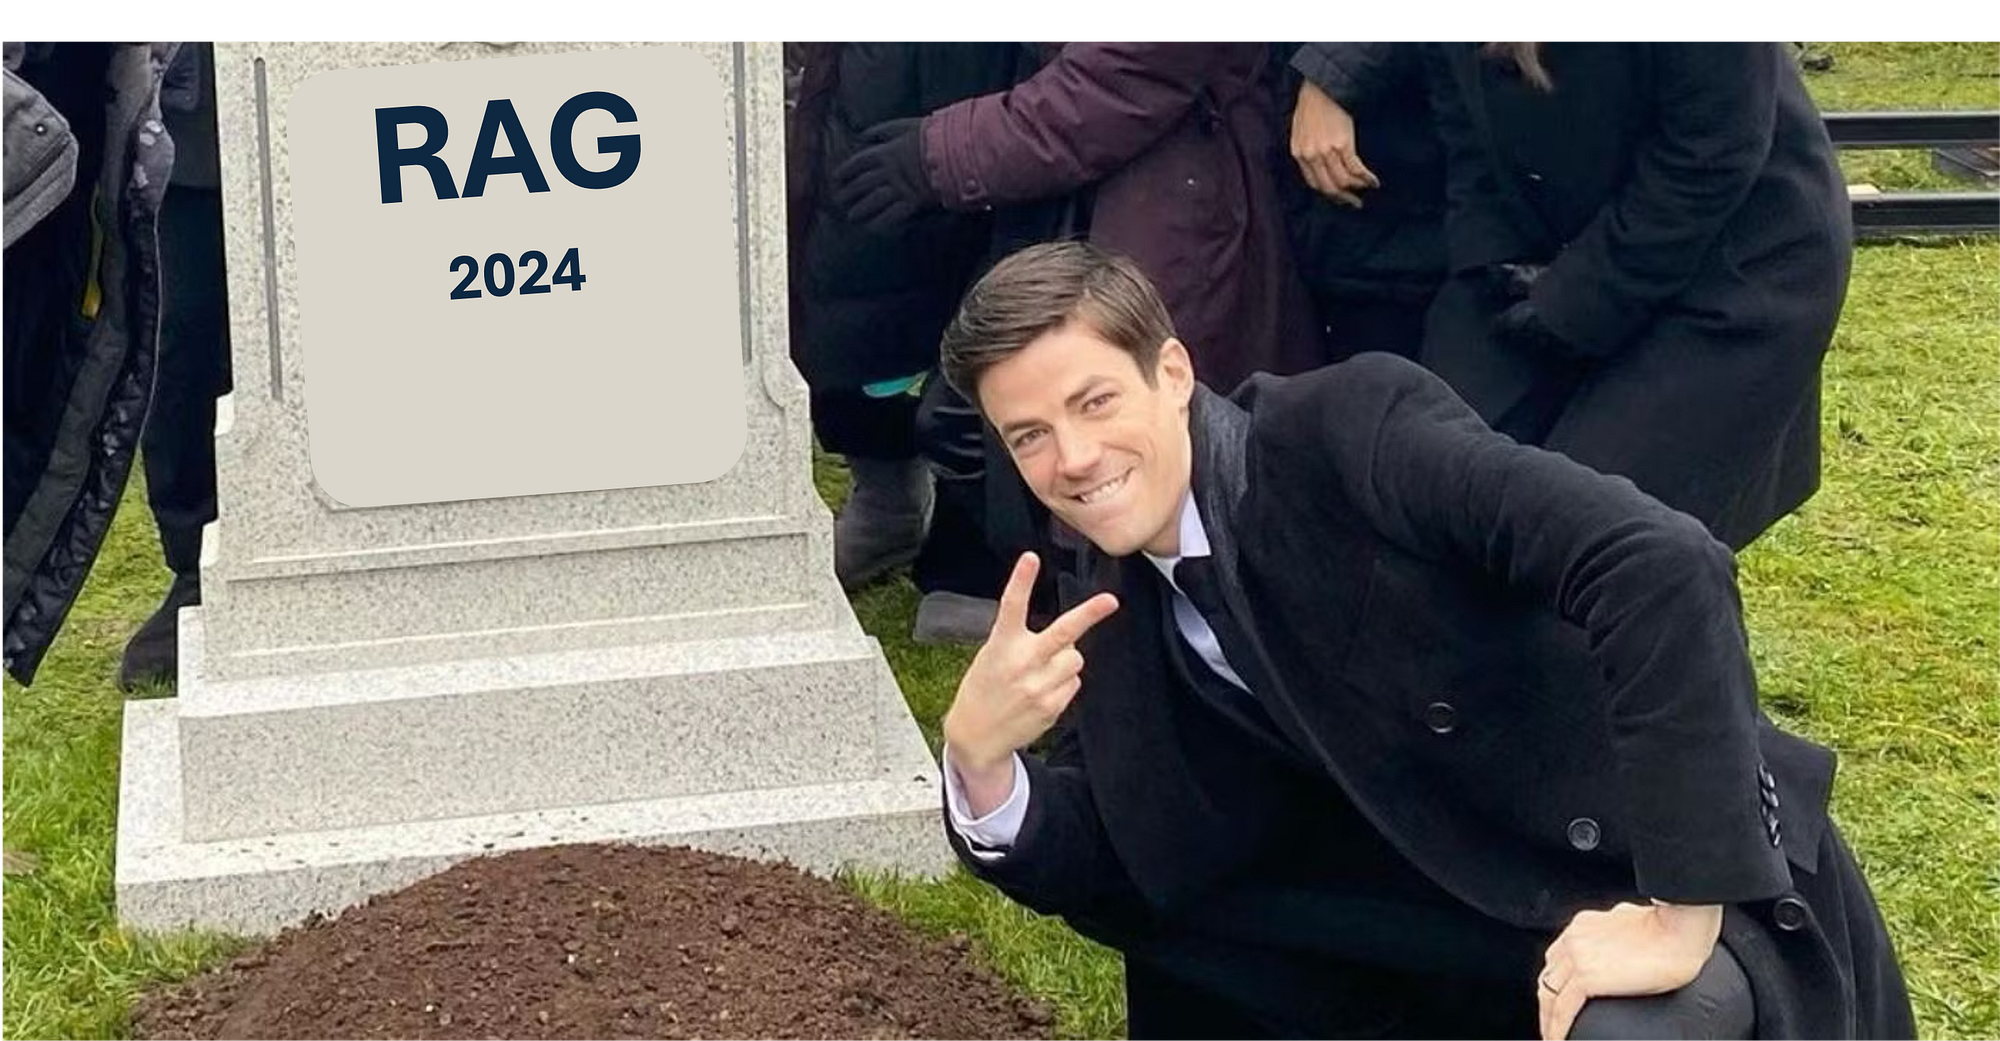
\includegraphics{images/misc/rag.png}
    \caption[RAG is dead meme]{Retrieval Augmented Generation (RAG) has been buried a dozen times according to LinkedIn AI influencers, replaced by agents, long context models, keyword search... In practice, models will change, but the need to condition a generative process on external information will remain very much alive.}

    % Latencies indicated in the figure are computed on the same machine \texttt{g2-standard-16} with a NVIDIA-L4 GPU, and averaged over 100 pages. Further details in \autoref{subsection:latency}.The computed score is the average of from all datasets in \textit{ViDoRe} for PDF Parser + Captioning and ColPali respectively. Further details in \autoref{section:results}.} 
    \label{fig:rag_dead}
\end{marginfigure}



At its core, indexing and retrieving information from external sources in a working "memory" is likely to remain one of the key challenges of AI systems in the future. Scientific advances will unlock better recall from broader sources and more personalized answers and the form factor will change, but the need to rely on external verifiable non-parametric resources to supplement our memory, and the need to \emph{navigate the maze} and separate information from noise will remain key.  

The parting words in Chapter \autoref{ch:conclusion} offer some personal perspectives into what I believe to be impactful future research directions in the retrieval field. In line with the rest of this thesis, I preach efforts into omni-modal universal embeddings, scaffolding engineering, reflect on ways to push benchmarking efforts forward, and detail why I believe bridging efforts with other NLP fields such as long context modeling research might enable scaling the training of embedding models multiple orders of compute magnitude. To anyone reading this thesis and wishing to discuss these ideas with me, my mail is open.


\section{List of Publications and Impact} 

This thesis is recollection of a focused selection of first-author\sidenote{I am last author on Vidore V2 and ModernVBert but was the one setting the research direction, closely supervising the projects and mostly writing the produced manuscripts} papers produced during the first 2.5 years of my PhD program. Most papers presented are inserted verbatim as chapters of the thesis and left unmodified with respects to the original peer-reviewed publication of the work. 


\noindent\textbf{Visual Document Retrieval.} The first part focuses on visual document retrieval, beginning with 
\emph{ColPali: Efficient Document Retrieval with Vision Language Models} 
\sidecite{faysse2025colpaliefficientdocumentretrieval}, published at ICLR 2025. It then turns to 
\emph{ModernVBERT: Towards Smaller Visual Document Retrievers} 
\sidecite{teiletche2025modernvbert}, published at ICML 2026, and to the ViDoRe benchmark series: 
\emph{ViDoRe Benchmark V2: Raising the Bar for Visual Retrieval} and 
\emph{ViDoRe V3: A Comprehensive Evaluation of Retrieval Augmented Generation in Complex Real-World Scenarios} 
\sidecite{macé2025vidorebenchmarkv2raising, loison2026vidorev3comprehensiveevaluation}, accepted at ACL 2026\sidenote{Although I initiated the project and was the original senior author, my role became more advisory towards the end as I joined the team at Meta FAIR working on unrelated topics for the last 6 months of my PhD.}. 


The contributions of this thesis go beyond a series of peer reviewed publications. Significant efforts were devoted to continuously improve the performance, to extend the capabilities and to advocate for the use of Visual Document Retrieval models. We can notably mention the release of the ColQwen model series\sidenote{We published the models openly and integrated the code on HuggingFace \url{https://huggingface.co/docs/transformers/main/model_doc/colqwen2}}, a series of SOTA visual retrievers, downloaded over 5 million times on HuggingFace at the time of writing. We also extended retrieval to other modalities such as video and audio through ColQwen-Omni \sidenote{We published the model openly on the HuggingFace platform and released a blog post at \url{https://huggingface.co/blog/manu/colqwen-omni-omnimodal-retrieval}.} and maintained the ColPali GitHub library at \url{https://github.com/illuin-tech/colpali}. The field of Visual Document Retrieval is now well established and thriving.



\noindent\textbf{Contextual Document Retrieval.} The second part focuses on leveraging contextual information to improve retrieval. It covers 
\emph{Context is Gold to find the Gold Passage: Evaluating and Training Contextual Document Embeddings} 
\sidecite{conti2025context}, accepted as an Oral at EMNLP 2025, and 
\emph{CroissantLLM: A Truly Bilingual French-English Language Model} 
\sidecite{faysse_croissantllm_2024}, published at TMLR 2025.

A FEW IMPACT METRICS ?

% exclude from thesis 

\noindent\textbf{Other First Author Papers.} Thesis manuscripts are focused by nature. My thesis itself was less so. Towards the end, a small section is dedicated to presenting a few papers linked to this main body of work. Notably, in "Self-Pruned Key Value Attention: Learning When To Write by Predicting Future Utility" \sidecite{szilvasy2026selfprunedkeyvalueattentionlearning} currently undergoing peer review, we tackle in-context retrieval problems through long context language modeling. Viewing a LLM KV Cache as a memory mechanism, we show we can induce the LLM to learn which information to store or discard, leading to reduced memory usage and improved speeds with no performance degradations. In another first author paper, "Revisiting Instruction  Model Evaluation" \sidecite{faysse2023revisiting} accepted as an Oral at EMNLP 2023, we show the benefits of using LLMs as judges for capability assessment. While this approach is now widespread\sidenote{Written in May 2023 and released in October 2023 after the EMNLP anonymity period, following the rules in place at the time.}, this paper was an early work advocating the use of LLM-based evaluation for broad capability measurement as they display strong task agnostic grading scales.
%The paper stems from the observation that instruction-tuned LLMs are deployed across an increasingly diverse set of tasks, making task-specific metrics difficult to maintain, poorly calibrated, and ultimately non-scalable. It shows that LLM judges can provide consistent signal across heterogeneous tasks and remain robust to variation in expected answer formats---settings where many traditional generative metrics fall short. The analysis further reveals distinct phases during supervised fine-tuning: models often learn to match the \emph{format} of the desired output before improving underlying task performance. Building on this finding, the work proposes leveraging synthetic data augmentation to improve data efficiency. Overall, this chapter argues for a fairer and more practical assessment of the capabilities of this new generation of models. Since the release of this work, LLM-as-a-judge methods have become a dominant approach for evaluating RAG systems and related techniques \sidecite{es2025ragasautomatedevaluationretrieval, kim2023prometheus, muller2025grousebenchmarkevaluateevaluators}.


\noindent\textbf{Other Papers.}  During this thesis, I also contributed as an active but secondary author to many other publications. Notably, in \sidecite{gisserotboukhlef2024trustworthyrerankingsimpleeffective} (TMLR 2024) we study whether the distribution of retrieval score can be leveraged to construct confidence estimations of retrieval performance. This idea of exploiting often unused information to improve retrieval is very related to the main body of this thesis's work. The confidence metrics have notably been integrated within the MTEB framework, as part of the MMTEB release which I am also a contributor of \sidecite{enevoldsen2025mmteb} (ICLR 2025). This thesis came at a time where open initiatives towards building multilingual LLMs were important and I participated in multiple such large projects following the success of CroissantLLM. Notably, with a team in Portugal, I worked on the EuroLLM series \sidecite{martins2024eurollmmultilinguallanguagemodels, martins2025eurollm} to train high performing open multilingual models with a special focus set on machine translation. I also contributed to an initiative to train improved multilingual bidirectional encoders which culminated in EuroBert \sidecite{boizard2025eurobert} (COLM 2025). With the EuroBert team, we further studied the differences between the training dynamics of encoder and decoder models in controlled setups, leading to \sidecite{gisserotboukhlef2025pretrainencodersmaskedlanguage}, under submission at ICLR 2026.

\noindent\textbf{ML Privacy Papers.} My early days of academic research were in the field of Computational Privacy. While I preferred focusing on LLMs and Information Retrieval during my thesis, privacy is a topic that stayed close to my heart. While working on CroissantLLM, I suggested to former colleagues that we could leverage this unique opportunity to also run LLM privacy research with huge LLM pretraining budgets. This led to a series of works, notably the Copyright Trap project \sidecite{meeus2024copyright} accepted at ICML 2024 in which we study model memorization of training data and draw conclusions into the risk of personal information leakage. A subsequent paper, \sidecite{meeus2024sok} provides a systematic  overview of membership inference attacks against LLM training data, organizing existing methods, clarifying threat models and assumptions, and highlighting open problems. It was awarded best paper award at IEEE SatML 2025. 

\noindent\textbf{Press \& Talks.}
Mention Press and Talks

\noindent\textbf{Ressource Releases.}
All models released as part of this thesis are openly released under open licenses.



\chapter{A Brief History of Information Retrieval}

While this thesis does not aim to provide an extensive overview of past or modern Information Retrieval techniques, the following section will provide a rapid overview of the field in order to contextualize the contributions of this thesis.\sidenote{If the reader finds this overview incomplete or yearns for more contextual depth, they are invited to search for further information within external sources. If the search is successful, great! If not, it only is further proof that modern search tools remain imperfect and that their improvement is a valid research motivation for this thesis.}
%\sidenote{As a disclaimer, this chapter is the only chapter of this thesis in which generative AI tools were used to assist redaction. All content is thoroughly verified.}. 
Further finely scoped relevant related work are also introduced in each individual chapters.


\section{Early Pre-Digital Cataloging}

\begin{marginfigure}
    \centering
    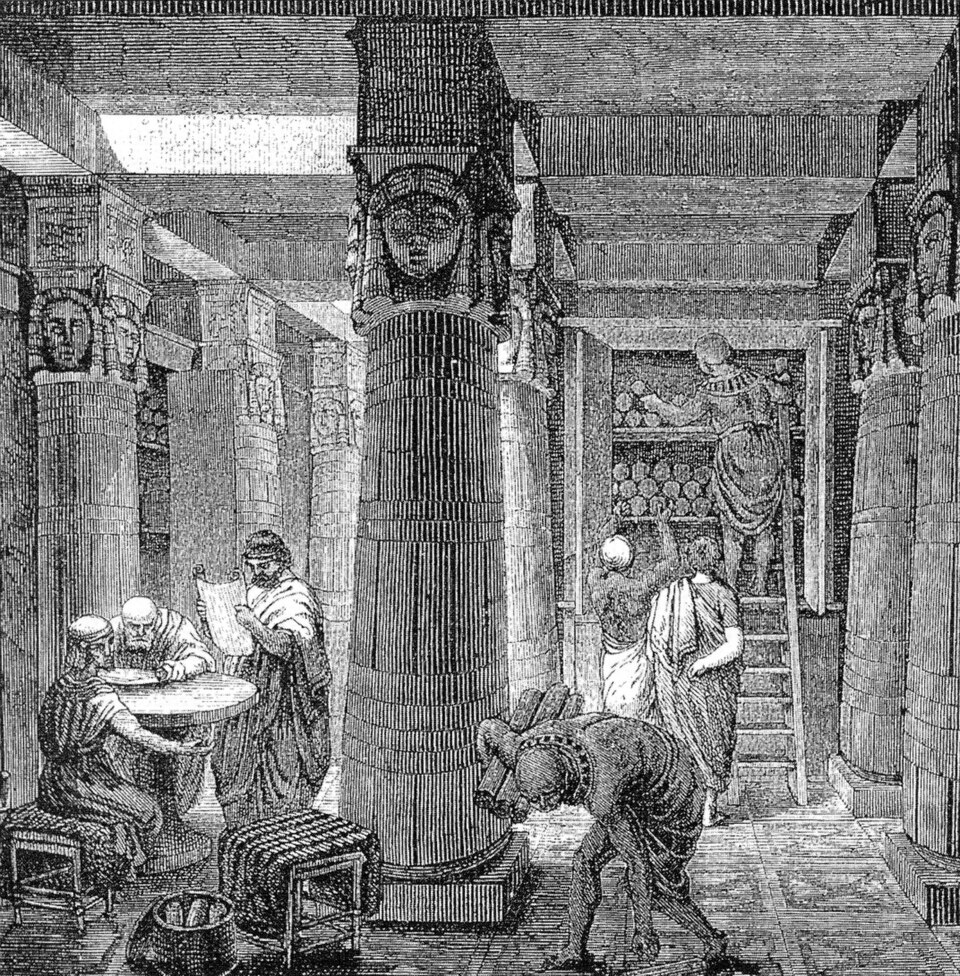
\includegraphics{images/misc/Ancientlibraryalex.jpg}
    \caption[Artistic Depiction of the Library of Alexandria based on historical evidence]{Artistic Depiction of the Library of Alexandria based on historical evidence. O. Von Corven -  "The Great Library of Alexandria"}

    % Latencies indicated in the figure are computed on the same machine \texttt{g2-standard-16} with a NVIDIA-L4 GPU, and averaged over 100 pages. Further details in \autoref{subsection:latency}.The computed score is the average of from all datasets in \textit{ViDoRe} for PDF Parser + Captioning and ColPali respectively. Further details in \autoref{section:results}.} 
    \label{fig:alexandria}
\end{marginfigure}

Long before computers, humans developed methods to organize and retrieve information. One of the earliest examples is the \emph{Pinakes} of Callimachus around the 3rd century BCE, often considered the first library catalog in the Western world. The \emph{Pinakes} is said to have systematically cataloged the authors and works held in the Library of Alexandria, organizing texts by subject and arranging authors alphabetically — an early bibliographic method that helped lay the foundations for later library catalogs. 

% This ancient effort demonstrated the enduring principles of indexing and categorization (such as alphabetical order and subject grouping) that remain fundamental in information retrieval (IR).


Through the centuries, librarians and scholars continued to develop catalogs and classification systems, from medieval manuscript indexes \sidecite{conraulewis_medieval_indices}
 to Melvil Dewey’s Decimal Classification in 1876 \sidecite{dewey1876classification}. These pre-digital innovations addressed the same core challenge as modern IR systems: \emph{how to store, organize, and find relevant information efficiently}. In 1945, Vannevar Bush articulated a technological vision for the future of information retrieval in \emph{As We May Think} \sidecite{bush1945aswemaythink}. He describes the inadequacy of indexing based systems to navigate the deluge of information:


\begin{lavenderkaobox}
"The real heart of the matter of selection, however, goes deeper than a lag in the adoption of mechanisms by libraries, or a lack of development of devices for their use. Our ineptitude in getting at the record is largely caused by the artificiality of systems of indexing. When data of any sort are placed in storage, they are filed alphabetically or numerically, and information is found (when it is) by tracing it down from subclass to subclass. It can be in only one place, unless duplicates are used; one has to have rules as to which path will locate it, and the rules are cumbersome."
\flushright -- Vannevar Bush, As We May Think (1945)
\end{lavenderkaobox}


Bush's vision was that new technology would enable moving away from this system. He proposes the \emph{Memex}, a hypothetical electromechanical desk that could instantly retrieve microfilmed documents via associative links. 
% Bush’s essay inspired later developments by suggesting that managing the “growing mountain of information” would require new mechanized solutions.

\section{Founding of Information Retrieval (1950s–1960s)}
Information Retrieval as a distinct field took shape in the 1950s and 1960s, alongside the advent of digital computers. In 1950, Calvin Mooers coined the term "information retrieval" \sidecite{mooers1950information}, heralding the idea of using machines to search document collections. Early experiments followed quickly: in 1951, a master’s thesis at MIT by Philip Bagley \sidecite{bagley1951electronic} demonstrated one of the first computerized document retrieval experiments. Pioneers like Hans Peter Luhn at IBM began applying computers to automate indexing; for example, Luhn developed methods for auto-encoding documents and keyword-in-context indexing. By 1959 he published an influential paper on “Auto-encoding of documents for information retrieval” \sidecite{luhn1959autoencoding} showing how computers could encode text and allow electronic searching of content. This period also saw growing support for IR research as the U.S. government recognized an information explosion funding projects on mechanized literature searching and the creation of citation indexes.


A key milestone was the Cranfield experiments led by Pete Cleverdon in the early 1960s \sidecite{cleverdon1967cranfield}. The Cranfield studies introduced a rigorous experimental methodology for IR: assembling a test collection of documents, queries, and relevance judgments, and evaluating retrieval performance using metrics like precision and recall. This methodology became a cornerstone of IR research, establishing a scientific approach to evaluate how “relevant” the results returned by an IR system are, laying the foundation for future benchmarks.
% The Cranfield approach was hard work (manually judging relevance for many query-document pairs), but it laid the foundation for future benchmarks.


During the same era, Gerard Salton formed the first major IR research group (at Harvard, later Cornell). Researchers began formulating the first theoretical models of IR. In 1960, Maron and Kuhns proposed a probabilistic indexing model \sidecite{maron1960relevance}, foreshadowing later probabilistic retrieval approaches. Salton and others started developing what became the vector space model: by the late 1960s, Salton’s team had created the SMART system, representing documents and queries as vectors in a term-weighted space. In 1968 Salton published “Automatic Information Organization and Retrieval” \sidecite{salton1968automatic} and by 1975 he fully articulated the vector space framework and term-weighting schemes \sidecite{salton1975vector_space}. Another 1960s contribution came from Karen Spärck Jones, who introduced the concept of inverse document frequency (IDF) \cite{sparck_jones_statistical_1972} to statistically downweight common terms and boost rare, informative terms – a principle that soon became central to ranking algorithms.

\section{The Statistical Revolution in IR (1970s--1990s)}

With the fundamentals laid, subsequent decades saw rapid improvement in statistical text retrieval methods. The 1970s refined the vector space and probabilistic models. Term frequency--inverse document frequency (TF--IDF) weighting became a standard technique: terms are scored higher if they appear frequently in a document (term frequency) but are rare across the collection (high IDF)\sidecite{sparck_jones_statistical_1972}\sidenote{
\textbf{TF-IDF:}
Let $\mathcal{D}=\{d_1,\dots,d_N\}$ be a corpus of $N$ documents and let $t$ be a term (token).
The TF--IDF weight of term $t$ in document $d$ is
\[
\mathrm{tfidf}(t,d,\mathcal{D}) \;=\; \mathrm{tf}(t,d)\cdot \mathrm{idf}(t,\mathcal{D}).
\]
A common choice is
\[
\mathrm{tf}(t,d)=\frac{f_{t,d}}{\sum_{t'} f_{t',d}}
\]
and
\[
\mathrm{idf}(t,\mathcal{D})=\log\!\left(\frac{N}{\mathrm{df}(t)}\right),
\]
where $f_{t,d}$ is the raw count of occurrences of $t$ in $d$, $\sum_{t'} f_{t',d}$ is the total number of term occurrences in $d$ (so $\mathrm{tf}$ is a normalized frequency),
and $\mathrm{df}(t)=\bigl|\{d_i\in\mathcal{D}: t\in d_i\}\bigr|$ is the document frequency (the number of documents containing $t$ at least once).
Intuitively, $\mathrm{tf}$ upweights terms frequent in a given document, while $\mathrm{idf}$ downweights terms that appear in many documents.
(Variants often use $\mathrm{tf}(t,d)=1+\log f_{t,d}$ and/or smoothing $\log\!\left(\frac{N+1}{\mathrm{df}(t)+1}\right)+1$ to avoid division by zero.)
}.  On the probabilistic side, Stephen Robertson and colleagues extended early ideas into the Probabilistic Relevance Framework in the 1970s and 1980s, leading to the development of ranking functions that estimate the probability a document is relevant to a query \sidecite{robertson1976relevance_weighting, robertson1977prp, robertson_probabilistic_2009}. These efforts culminated in the 1990s with Okapi BM25, developed in the Okapi/TREC line of work from the Robertson--Sp{\"a}rck Jones probabilistic framework and Robertson--Walker 2-Poisson approximations \sidecite{robertson1994bm25, robertson_okapi_1994}\sidenote{\textbf{BM25:}
Let $\mathcal{D}$ be a corpus, $d\in\mathcal{D}$ a document, and $t$ a term. The BM25 score of $d$ for a query $q$ is
\[
\mathrm{BM25}(q,d)=
\]
\[
\sum_{t\in q} \mathrm{idf}(t)\;
\frac{f_{t,d}(k_1+1)}{f_{t,d}+k_1\!\left(1-b+b\,\frac{|d|}{\mathrm{avgdl}}\right)}
\]
Here $f_{t,d}$ is the count of $t$ in $d$, $|d|$ is the document length (in tokens), and $\mathrm{avgdl}$ is the average document length in the corpus. $k_1>0$ controls term-frequency saturation, and $b\in[0,1]$ controls how strongly length normalization is applied. A common IDF is
\[
\mathrm{idf}(t)=\log\!\left(\frac{N-\mathrm{df}(t)+0.5}{\mathrm{df}(t)+0.5}\right),
\]
where $N=|\mathcal{D}|$ and $\mathrm{df}(t)$ is the number of documents containing $t$.
}. 
By incorporating TF--IDF-like features into a probabilistic model, BM25 became one of the dominant ranking algorithms in search and remains widely used as a strong baseline in modern information retrieval systems \sidecite{robertson_probabilistic_2009, manning2008introduction_ir}.

Alongside algorithm advances, IR systems grew in scale and importance. The first online search systems appeared in the early 1970s as databases of bibliographic records: for example, MEDLINE (1971) provided biomedical literature search, and DIALOG offered commercial online search over multiple databases \sidecite{nlm2024medline_history, dialog2019milestone}. These systems predated personal computers---users accessed them via terminals---but they demonstrated that searching thousands of documents via text queries was feasible and valuable. In 1978, the IR community established its premier conference, ACM SIGIR, reflecting the field's maturation \sidecite{sigir1978proceedings}.

By the 1980s, personal computing and CD-ROMs enabled standalone IR systems (like library catalog CDs), and researchers explored new ideas such as relevance feedback (the Rocchio algorithm from the 1970s allowed a system to adjust a query based on documents a user marked relevant) \sidecite{rocchio1971relevance_feedback} and clustering (the "cluster hypothesis": relevant documents tend to cluster together)\sidecite{jardine1971hierarchic_clustering, vanrijsbergen1979information_retrieval}. The inverted index (storing, for each term, a list of documents containing it) became a core data structure, enabling fast keyword lookup even as collections grew to tens of thousands of documents \sidecite{manning2008introduction_ir}. This era also saw experiments with user interfaces and visualization (e.g.\ plotting document similarity or using hypertext systems).

Evaluation at scale took a leap in 1992 with the start of the Text Retrieval Conference (TREC). TREC built large standard test collections and yearly competitions for state-of-the-art retrieval methods \sidecite{harman1993trec_overview}. TREC not only pushed research towards scalable methods but also fostered the development of specialized tasks. Many techniques that became important, such as query expansion and relevance feedback, were evaluated and refined through TREC workshops.

Web search emerged in the mid-1990s as a new frontier that dramatically expanded IR's scale and impact. Early web search systems and directories---for example, Yahoo!'s human-curated directory in 1994 and AltaVista in 1995---helped users navigate the growing World Wide Web, but human-maintained directories were difficult to scale and keyword-based engines often returned many low-quality matches at web scale\sidecite{brin1998anatomy}.

A major breakthrough came from the Stanford/Google work of the late 1990s, especially PageRank, which treated the web as a graph and used hyperlinks as an additional ranking signal: a page linked from many other pages, especially pages that were themselves important, received a higher importance score\sidecite{page1998pagerank, brin1998anatomy}. By combining link analysis with content relevance, anchor text, proximity, and other web-specific signals, Google produced more useful rankings than many earlier content-only systems\sidecite{brin1998anatomy}. This represented a graph-based retrieval innovation, leveraging network topology in a way analogous to citation analysis in scholarly literature.

In the 2000s, machine learning techniques became increasingly central to IR. Learning-to-rank algorithms learned how to combine many ranking features---such as lexical matching scores, anchor-text evidence, document features, and user-behavior-derived signals---into ranking functions\sidecite{burges2005ranknet, burges2006lambdarank, burges2010lambdamart}. Microsoft Research developed RankNet and LambdaRank in the mid-2000s, with LambdaMART later combining LambdaRank-style optimization with boosted decision trees\sidecite{burges2005ranknet, burges2006lambdarank, burges2010lambdamart}. Commercial search engines increasingly incorporated machine-learned ranking methods, although the exact algorithms and deployment timelines were often proprietary.

Researchers also showed that clickthrough logs and query reformulations could provide useful implicit feedback for ranking, though clicks are biased and must be interpreted carefully rather than treated as direct relevance judgments\sidecite{joachims2002clickthrough, joachims2005clickthrough, radlinski2005query_chains}.

Another 2000s-and-2010s trend was the use of semantic information and knowledge bases. For instance, Bing publicly described its Satori knowledge system in 2013 as modeling entities---people, places, and things---and relationships among them\sidecite{bing2013satori}. Google also moved in this direction through systems such as the Knowledge Graph and, in 2013, Hummingbird, a major improvement to its ranking systems associated with better handling of longer and more conversational queries\sidecite{google2025ranking_systems}.

\section{The Deep Learning Era of IR (2010s--2020s)}

The 2010s shifted information retrieval from purely lexical matching toward neural semantic matching. Early neural IR systems such as DSSM mapped queries and documents into learned vector spaces, allowing systems to match texts that used different words but expressed related meanings\sidecite{huang2013dssm}. This was the beginning of dense retrieval: instead of representing a document only by the terms it contains, the system learns a continuous embedding that captures semantic similarity.

The transformer era accelerated this shift. BERT showed that large pretrained language models could produce rich contextual representations of text,\sidecite{devlin2019bert} and by 2019 Google had publicly announced the use of BERT in Search to better handle longer, more conversational queries\sidecite{google2019bert_search}. In academic IR, BERT-style cross-encoders became especially effective as rerankers: a first-stage retriever such as BM25 or a dense retriever retrieves a candidate set, and a neural model then scores each query--document pair more precisely\sidecite{nogueira_passage_2019, yates2021transformers_ranking}.

At the same time, researchers developed neural retrievers that could operate efficiently at first stage. Bi-encoders or dual encoders represent queries and documents independently, so retrieval can be performed through nearest-neighbor search in vector space\sidecite{karpukhin2020dpr}. Sentence-BERT made BERT-style sentence embeddings practical for semantic similarity and retrieval,\sidecite{reimers2019sbert} while DPR showed that dense passage retrieval could outperform BM25 on several open-domain question-answering benchmarks\sidecite{karpukhin2020dpr}. Late-interaction models such as ColBERT offered a middle ground: they retained token-level matching signals while remaining much more efficient than full cross-encoder reranking\sidecite{khattab2020colbert}.

By the early 2020s, the dominant neural IR architecture had become multi-stage: a fast lexical, sparse, or dense retriever produces candidates; a stronger neural reranker refines them; and systems often combine lexical and semantic signals rather than replacing one with the other\sidecite{yates2021transformers_ranking}.



\section{The Modern Stack: Hybrid, Contextual, and Agentic Retrieval}

Modern IR is no longer a simple competition between BM25 and dense vectors. High-performing systems increasingly combine multiple retrieval signals: lexical matching for exact terms, dense embeddings for semantic similarity, learned sparse models for interpretable expansion, late-interaction models for token-level matching, and cross-encoders or LLM rerankers for final precision.

A first trend is the rise of general-purpose embedding models. Models such as GTE train unified text embeddings with multi-stage contrastive learning over diverse datasets,\sidecite{li2023generaltextembeddingsmultistage} while E5-style models and E5-Mistral show that strong embedding models can be built by adapting large language models and training on large synthetic instruction-style data\sidecite{wang2024improvingtextembeddingslarge}. More recent work directly adapts decoder-only LLMs into embedding models: LLM2Vec converts causal LLMs into bidirectional text encoders through bidirectional attention, masked next-token prediction, and contrastive learning,\sidecite{behnamghader_llm2vec_2024} while NV-Embed introduces practical techniques such as latent-attention pooling, removing the causal mask during contrastive training, and two-stage instruction tuning\sidecite{lee2024nvembedimprovedtechniquestraining}. NV-Retriever further highlights the importance of hard-negative mining, especially positive-aware methods that reduce false negatives during contrastive learning\sidecite{moreira2024nvretriever}.

A second trend is the return of sparse retrieval in neural form. Learned sparse models preserve the operational advantages of inverted indexes while learning term expansion and weighting from data. SPLADE is a representative example: it learns sparse lexical representations using explicit sparsity regularization and log-saturated term weights, making it suitable for first-stage retrieval with inverted indexes\sidecite{10.1145/3404835.3463098}. More recent work pushes this idea beyond vocabulary terms. Sparse-autoencoder-based retrieval models such as SPLARE learn sparse latent embeddings from LLM representations, aiming for more semantic and multilingual sparse features\sidecite{formal2026learningretrievalmodelssparse}. The Latent Terms line of work similarly shows that dense retrievers can contain extractable sparse, BM25-ready latent features, suggesting that dense and sparse retrieval may be less separate than they first appear\sidecite{latentterms}.

A third trend concerns context. Standard chunking pipelines often split documents before embedding them, which can remove surrounding context from each chunk. Late Chunking reverses this order: it first encodes a longer text with a long-context embedding model, then pools token representations into chunk embeddings, allowing chunk vectors to retain information from the broader document\sidecite{LateChunking}. Contextual Document Embeddings extend the same idea to corpora: a document representation can be improved by considering neighboring or related documents rather than encoding each document in isolation\sidecite{morris2024contextualdocumentembeddings}. This matters especially for RAG systems, where the quality of retrieved chunks can depend on information outside the chunk itself.

A fourth trend is more expressive scoring. Dense retrieval usually scores a query and document by a dot product or cosine similarity between vectors, which is efficient but limits the kinds of relevance functions that can be represented. Hypencoder proposes a different paradigm: the query encoder produces a small neural network that scores document representations, allowing query-specific relevance functions while still supporting approximate retrieval\sidecite{killingback2025hypencoderhypernetworksinformationretrieval}. This illustrates a broader movement beyond fixed-vector similarity toward richer, task-adaptive scoring mechanisms.

Finally, retrieval is becoming agentic and reasoning-aware. Classical search assumes a user issues a query and receives a ranked list. Modern LLM-based systems often plan, decompose a task, issue multiple searches, inspect evidence, and reformulate queries. ReasonIR trains retrievers specifically for reasoning-intensive tasks, using synthetic data that pairs challenging queries with relevant documents and hard negatives\sidecite{shao2025reasonir}. AgentIR goes further by treating deep-research agents as retrieval users: instead of embedding only the final query, it embeds the agent's reasoning trace together with the query, so the retriever can exploit the agent's expressed intent\sidecite{chen2026agentir}. In this view, IR is no longer just document ranking; it becomes part of a larger reasoning loop involving query planning, retrieval, reranking, evidence synthesis, and attribution.


% \section{Engineering}
% FAISS,

% \section{Industrial Applications}

% RAG, word extraction



\pagelayout{wide} % No margins
\addpart{Visual Document Retrieval}
\pagelayout{margin} % Restore margins


\setchapterpreamble[u]{\margintoc}
\chapter{\textit{ColPali}: Efficient Document Retrieval with Vision Language Models}

% \begin{figure*}[ht] 
%     \centering
% ¡    \includegraphics[width = 0.95\textwidth]{images/colpali_images/architecture.png}
%     \caption{}
%     \label{fig:colpali_architecture}
% \end{figure*}
\begin{kaobox}[frametitle=Paper Abstract]


Documents are visually rich structures that convey information through text, but also figures, page layouts, tables, or even fonts. Since modern retrieval systems mainly rely on the textual information they extract from document pages to index documents -often through lengthy and brittle processes-, they struggle to exploit key visual cues efficiently. This limits their capabilities in many practical document retrieval applications such as Retrieval Augmented Generation (RAG).
To benchmark current systems on visually rich document retrieval, we introduce the Visual Document Retrieval Benchmark \textit{ViDoRe}, composed of various page-level retrieval tasks spanning multiple domains, languages, and practical settings. 
The inherent complexity and performance shortcomings of modern systems motivate a new concept; doing document retrieval by directly embedding the images of the document pages. We release \textit{ColPali}, a Vision Language Model trained to produce high-quality multi-vector embeddings from images of document pages. Combined with a late interaction matching mechanism, \textit{ColPali} largely outperforms modern document retrieval pipelines while being drastically simpler, faster and end-to-end trainable. 
We release models, data, code and benchmarks under open licenses at \url{https://hf.co/vidore}.


\end{kaobox}


\section{Introduction}

Document Retrieval consists of matching a user query to relevant documents in a given corpus. It is central to many widespread industrial applications, either as a standalone ranking system (search engines) or as part of more complex information extraction or Retrieval Augmented Generation (RAG) pipelines.

%\vspace{0.1cm}
% Historically, statistical methods based on word frequencies were used (e.g. TF-IDF \sidecite{sparck_jones_idf_2004}, BM25 \sidecite{robertson_probabilistic_2009}), enabling offline corpus indexation in sparse vector sets, and fast query matching at inference time. With the advent of neural networks, stronger dense embedding models were developed by fine-tuning pre-trained language models with contrastive training objectives \sidecite{cer_universal_2018,reimers_sentence-bert_2019,gao_simcse_2021}. 


% Although text embedding models for query-passage retrieval have greatly improved over recent years, notably enabled by the rise of pretrained language models, the main bottleneck for efficient document retrieval in a practical industrial setting lies \textit{a priori}, in the way text passages to be embedded are constructed.

\noindent Over recent years, pretrained language models have enabled large improvements in text embedding models. In practical industrial settings, however, the primary performance bottleneck for efficient document retrieval stems not from embedding model performance but from the prior data ingestion pipeline. Indexing a standard PDF document involves several steps. First, PDF parsers or Optical Character Recognition (OCR) systems are used to extract words from the pages. Document layout detection models can then be run to segment paragraphs, titles, and other page objects such as tables, figures, and headers. A chunking strategy is then defined to group text passages with some semantical coherence, and modern retrieval setups may even integrate a captioning step to describe visually rich elements in a natural language form, more suitable for embedding models. 
% This leads to ingestion pipelines that are lengthy, require heavy parametrization, and orchestrate independent subsystems. 
In our experiments (\autoref{table:colpali:results}), we typically find that optimizing the ingestion pipeline yields much better performance on visually rich document retrieval than optimizing the text embedding model.


% The race to ever-more performant text embedding models should perhaps not be the only focus of research in the retrieval space.

% pipeline usually starts with a rotation correction model. Then comes the Optical Character Recognition (OCR) task: a text detection model locates the character/word bounding boxes (e.g. \texttt{crnn\_vgg16\_bn} \sidecite{shi_end--end_2015}, \texttt{LinkNet} \sidecite{chaurasia_linknet_2017}, \texttt{TextNET \sidecite{chen_fast_2021}}) and a text recognition model predicts the strings associated the words in the previously detected bounding boxes (e.g. \texttt{db\_resnet50}, \texttt{db\_mobilenet\_v3\_large} \sidecite{liao_real-time_2019}, \texttt{sar\_resnet31} \sidecite{li_show_2018}). Finally, specialized models or heuristics to determine the reading order to segment pages into titles and paragraphs \sidecite{huang_layoutlmv3_2022,meunier_optimized_2005}, to detect images and tables \sidecite{smock_pubtables-1m_2021,qiao_lgpma_2021,li_dit_2022,ge_yolox_2021} in order to process them separately, and finally to split documents into optimized text chunks to be embedded. The whole process can be lengthy, and its sequential nature propagates errors from earlier systems downstream. Moreover, it is non-differentiable and requires heavy parametrization efforts to optimize the deployment infrastructures. Finally, it is unclear how to best represent visually rich document objects such as tables, figures, and images \sidecite{zha_tablegpt_2023,gao_retrieval-augmented_2023}. In practice, they are often overlooked, although recently, some captioning strategies have been shown to be effective, although very resource-intensive during indexation.

\noindent\textbf{Contribution 1: \textit{ViDoRe}.}
In this work, we argue that document retrieval systems should not be evaluated solely on the capabilities of text embedding models \sidecite{bajaj_ms_2016,thakur_beir_2021, muennighoff_mteb_2022}, but should also consider the context and visual elements of the documents to be retrieved. To this end, we create and openly release \textit{ViDoRe}, a comprehensive benchmark to evaluate systems on page-level document retrieval with a wide coverage of domains, visual elements, and languages. \textit{ViDoRe} addresses practical document retrieval scenarios, where queries often necessitate both textual and visual understanding for accurate document matching. We highlight the shortcomings of current text-centric systems in these settings.\sidenote{The \textit{ViDoRe} benchmark leaderboard is hosted publicly at \url{https://huggingface.co/spaces/vidore/vidore-leaderboard} to encourage further developments.}

% \url{https://huggingface.co/spaces/<anonymous>}

\noindent\textbf{Contribution 2: \textit{ColPali}.}
We propose a novel concept and model architecture based on Vision Language Models (VLMs) to efficiently index documents purely from their visual features, allowing for subsequent fast query matching with late interaction mechanisms \sidecite{khattab_colbert_2020}. Our method, \textit{ColPali}, significantly outperforms all other retrieval systems on \textit{ViDoRe} while being fast and end-to-end trainable.
These results demonstrate the potential and the many benefits of this novel \textit{Retrieval in Vision Space} concept, which could significantly alter the way document retrieval is approached in the industry moving forward.
We release all resources at \url{https://hf.co/vidore}.

% \url{https://hf.co/<anonymous>}

% We argue this has the potential to revolutionize
% \sidenote{All project artifacts are openly released at \url{.com}.}.

% pour moi overclaim. New method =`> des insights. Ca fait croqueur
% \textbf{Contribution 3.}
% We run ablations to better understand the impact of our modeling choices on the retrieval performances. This unlocks insights into the trade-offs between model size and the number of image patches, as well as informs on the impact of design decisions, such as locked-image tuning, memory tokens, loss functions, etc...

% \textbf{Contribution 4.}
% We release our fine-tuned models and training code under open licenses, bringing to both researchers and industry practitioners state-of-the-art document retrieval models\sidenote{\url{huggingface.co/anon}}. We also release all artifacts related to benchmarking\sidenote{\url{github.com/anon}} (data, evaluation code, public leaderboards, reproducible baselines) to serve as a new reference for Document Retrieval.

\begin{figure*}
    \centering
    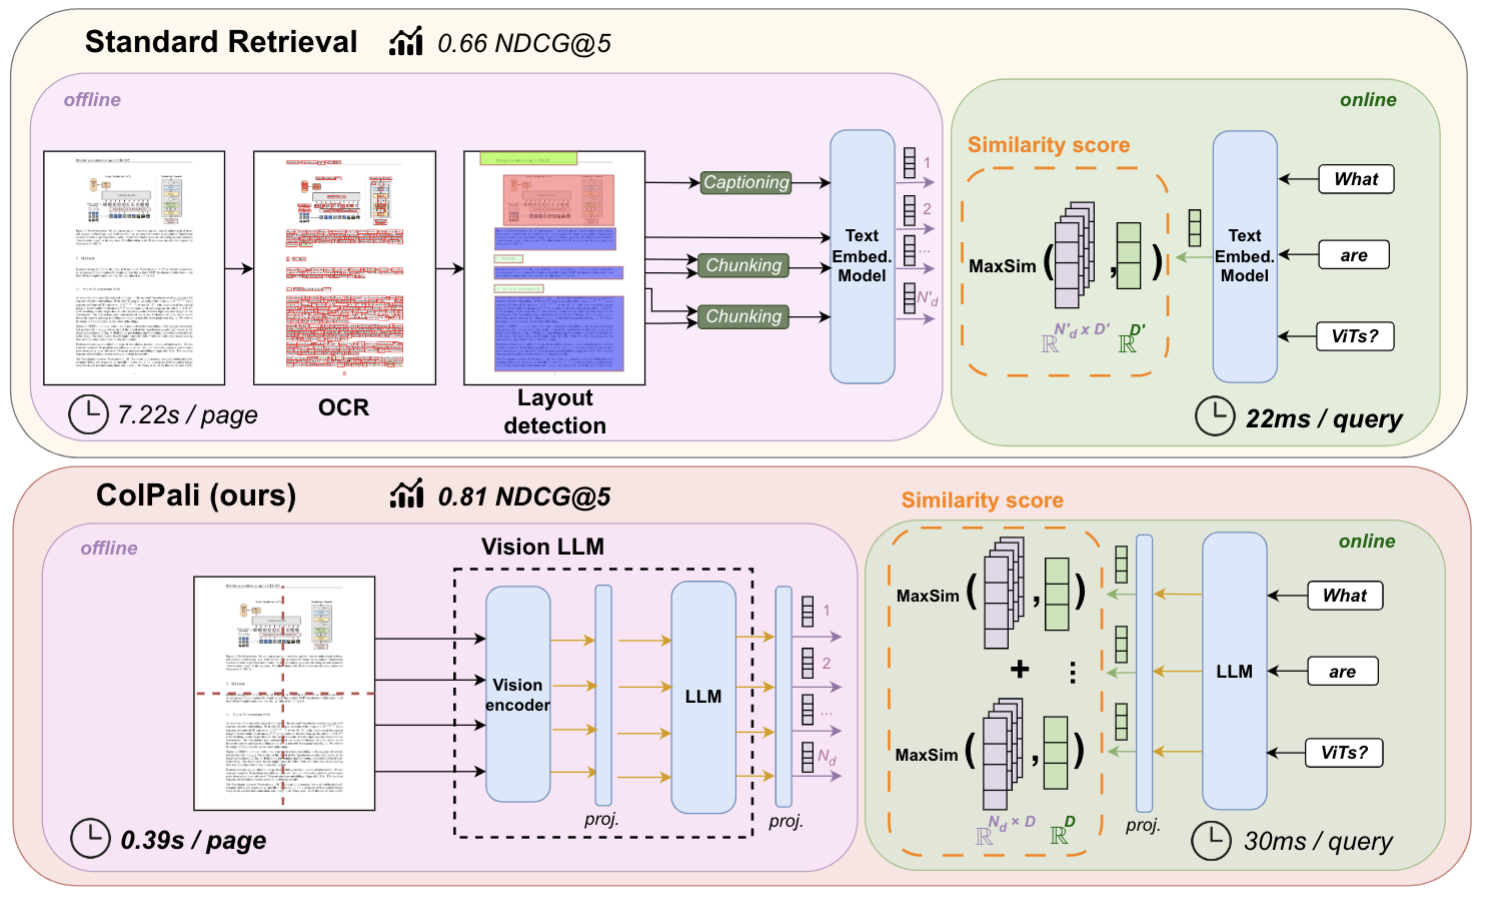
\includegraphics[width = 1.2\textwidth]{images/colpali_images/final_architecture.png}
    \caption[\textit{ColPali} overview]{\textit{ColPali} simplifies document retrieval w.r.t. standard retrieval methods while achieving stronger performances with better latencies. Latencies and results are detailed in \autoref{section:colpali:results} and \autoref{paragraph:latency_app}.}
    
    % Latencies indicated in the figure are computed on the same machine \texttt{g2-standard-16} with a NVIDIA-L4 GPU, and averaged over 100 pages. Further details in \autoref{subsection:latency}.The computed score is the average of from all datasets in \textit{ViDoRe} for PDF Parser + Captioning and ColPali respectively. Further details in \autoref{section:results}.} 
    \label{fig:colpali_architecture}
\end{figure*}


\section{Problem Formulation \& Related Work}

% Pierre
\noindent\textbf{Problem Setting.}
In our setting, a retrieval system scores how relevant a document $d$ from corpus $\mathcal{D}$ is with respect to a query $q$. Computing the similarity score $s(q, d) \in \mathbb{R}$ for each of the $|\mathcal{D}|$ documents in the corpus creates a ranking we can use to extract the most relevant documents. In this work, we focus on page-level retrieval: \textit{given a query, is the correct document page retrieved by the system?} For coherence with existing literature, we further use the term \textit{document} to refer to individual pages, i.e.\ the atomic retrieved elements in our setting. As we focus on practical industrial retrieval applications (RAG, search engines) with potentially large corpora sizes, latency constraints are imposed on scoring systems. Most current retrieval systems can be decomposed into (1) an \textit{offline} indexation phase in which a document index is built and (2) an \textit{online} querying phase in which a query is matched to documents from the index and where low latency is vital to the user experience. 

% \noindent\textbf{Efficient document retrieval systems exhibit joint properties of high retrieval performance (R1), low latency during querying (R2), and high throughput during indexation (R3).}

\label{subsec:constraints}
\noindent\textit{Under these industrial constraints, we identify three main properties an efficient document retrieval systems should exhibit: \textbf{(R1) strong retrieval performance}, as measured by standard retrieval metrics; \textbf{(R2) fast online querying}, measured through average latencies; \textbf{(R3) high throughput corpus indexation}, ie. the number of pages that can be embedded in a given timeframe.}


\subsection{Textual Retrieval Methods}
\noindent\textbf{Document Retrieval in Text Space.}

Statistical methods based on word frequency like TF-IDF \sidecite{sparck_jones_statistical_1972} and BM25 \sidecite{robertson_okapi_1994} are still widely used due to their simplicity and efficiency. More recently, neural embedding models based on fine-tuned large language models display state-of-the-art performance on a variety of text embedding tasks and top the retrieval leaderboards \sidecite{muennighoff_mteb_2022}. 

\noindent\textbf{Neural Retrievers.}
In bi-encoder models \sidecite{reimers_sentence-bert_2019, karpukhin_dense_2020, wang_text_2022}, documents are independently mapped \textit{offline} to a dense vector space. Queries are embedded \textit{online} and matched to documents through a fast cosine distance computation.
A slower, but slightly more performant alternative, cross-encoder systems \sidecite{wang_minilm_2020, cohere_introducing_2024} concatenate query and document as a single input sequence and iteratively attribute matching scores to each possible combination. This enables full attention computation between query and document terms but comes at the cost of computational efficiency, as $|\mathcal{D}|$ encoding passes must be done online.


\noindent\textbf{Multi-Vector retrieval via late interaction.}
In the late interaction paradigm introduced by ColBERT \sidecite{khattab_colbert_2020}, an embedding is pre-computed and indexed per document token. At runtime, similarity can be computed with individual query token embeddings. The idea is to benefit from the rich interaction between individual query and document terms while taking advantage of the offline computation and fast query matching enabled by bi-encoders. See \autoref{subsection:glossary_colbert} for more details.

% introduces the late interaction paradigm, which consists of handling independent multi-vector representations of the query and the document. This method offers ColBERT two advantages. First, being able to compute the representation of the documents prior to the query (\textit{late interaction}) makes it suitable for offline document indexing, thus reducing latency at query time. On the other hand, the decision of having a document represented by not one but a sequence of vectors allows to fully leverage the expressiveness of the neural text encoder.

% Although benchmarks and leaderboards have been developed to evaluate these text embedding models (MTEB, BEIR), most of the performance improvements in practical use cases of embedding models depend on the prior data ingestion pipeline (OCR, layout detection, chunking strategies) and we believe end-to-end evaluation is crucial to accurately close the gap between academic model benchmarks and industrial performance.

\noindent\textbf{Retrieval Evaluation.}
Although benchmarks and leaderboards have been developed to evaluate text embedding models \sidecite{thakur_beir_2021, muennighoff_mteb_2022}, much of the performance improvements in industrial use cases of embedding models stem from the prior data ingestion pipeline. While documents often rely on visual elements to more efficiently convey information to human readers, text-only systems barely tap into these visual cues. Other work has also independently studied table or chart retrieval systems through repurposed Question Answering datasets \sidecite{Zhang_2019, nowak-etal-2024-multimodal} but only assessing specialized methods for each task.

\noindent\textit{To our knowledge, no benchmark evaluates document retrieval systems in practical settings; in an end-to-end manner, across several document types and topics, and by evaluating the use of both textual and visual document features.}



\subsection{Integrating Visual features}

\noindent\textbf{Contrastive Vision Language Models.}
Mapping latent representations of textual content to corresponding representations of visual content has been done by aligning disjoint visual and text encoders through contrastive losses \sidecite{radford_learning_2021, zhai_sigmoid_2023}. While some OCR capabilities exist in these models, the visual component is often not optimized for text understanding. 

The Fine-grained Interactive Language-Image Pre-training \sidecite{yao_filip_2021} framework extends the late interaction mechanism to cross-modal Vision Language Models, relying on max similarity operations between text tokens and image patches.


\noindent\textbf{Visually Rich Document Understanding.}
% While the document signal can be found in tables, images, and figures, it is also found in the document layout or even font sizes and colors. 
To go beyond text, some document-focused models jointly encode text tokens alongside visual or document layout features \sidecite{appalaraju_docformer_2021, kim_ocr-free_2021, huang_layoutlmv3_2022, tang_unifying_2022}. 
Large Language transformer Models (LLMs) with strong reasoning capabilities have recently been combined with Vision Transformers (ViTs) \sidecite{dosovitskiy_image_2020} to create VLMs \sidecite{alayrac_flamingo_2022, liu_visual_2023, bai_qwen-vl_2023, laurencon_what_2024} where image patch vectors from contrastively trained ViT models \sidecite{zhai_sigmoid_2023} are fed as input embeddings to the LLM and concatenated with the text-token embeddings. 

\label{paragraph:generative_vision_language_model}
\noindent\textbf{PaliGemma.}
The PaliGemma-3B model \sidecite{beyer2024paligemmaversatile3bvlm} extends concepts from Pali3 \sidecite{chen_pali-3_2023}, and projects \texttt{SigLIP-So400m/14} \sidecite{alabdulmohsin_getting_2023} patch embeddings into Gemma-2B's text vector space \sidecite{gemma_team_gemma_2024}. Along with its reasonable size w.r.t. other performant VLMs, an interesting property of PaliGemma's text model is that it is fine-tuned with full-block attention on the prefix (instruction text and image tokens). See \autoref{section:model_glossary} for more details.

\noindent\textit{VLMs display enhanced capabilities in Visual Question Answering, captioning, and document understanding \sidecite{yue_mmmu_2023}, but are not optimized for retrieval tasks.}



\section{The \textit{ViDoRe} Benchmark}
\label{section:docvis_benchmark}

Existing benchmarks for contrastive vision-language models primarily evaluate retrieval for natural images \sidecite{lin_microsoft_2014,borchmann_due_2021,thapliyal_crossmodal-3600_2022}. On the other hand, textual retrieval benchmarks \sidecite{muennighoff_mteb_2022} are evaluated at at textual passage level and are not tailored for document retrieval tasks. We fill the gap with \textit{ViDoRe}, a comprehensive benchmark for document retrieval using visual features. 

\subsection{Benchmark Design}
\textit{ViDoRe} is designed to comprehensively evaluate retrieval systems on their capacity to match queries to relevant documents at the page level. This benchmark encompasses multiple orthogonal subtasks, with focuses on various modalities - text, figures, infographics, tables; thematic domains - medical, business, scientific, administrative; or languages - English, French. Tasks also span varying levels of complexity, in order to capture signals from both weaker and stronger systems.  
As many systems require large amounts of time to index pages (captioning-based approaches can take dozens of seconds per page for instance), we limit the number of candidate documents for each retrieval task in order to evaluate even complex systems in a reasonable timeframe without sacrificing quality. For trainable retrieval systems, we provide a reference training set that can be used to facilitate comparisons.
% Introduce the idea that some tasks are tougher than others


\begin{table}[ht]
    \centering
    \label{tab:docvisbench}
    \small
    \begin{tabular}{lllll}
        \toprule
        \textbf{Dataset} & \textbf{Language} & \textbf{\# Queries} & \textbf{\# Documents} &\textbf{Description}\\
        \midrule
        \textbf{Academic Tasks} & &\\
        DocVQA   &English  &  500 &500 & Scanned documents from UCSF Industry   \\
        InfoVQA  &English & 500 &500 & Infographics scrapped from the web\\
        TAT-DQA  &English  & 1600& 1600 & High-quality financial reports\\
        arXiVQA  &English & 500 &500& Scientific Figures from arXiv\\
        TabFQuAD &French & 210& 210  & Tables scrapped from the web \\
        \midrule
        \textbf{Practical Tasks} & \\
        Energy &English & 100 &1000 & Documents about energy\\
        Government &English & 100 &1000 & Administrative documents\\
        Healthcare &English &  100 &1000& Medical documents\\
        AI &English & 100 &1000 & Scientific documents related to AI\\
        Shift Project &French & 100 &1000 & Environmental reports\\
        \bottomrule
    \end{tabular}
    \caption[ViDoRe benchmark overview]{\textit{ViDoRe} comprehensively evaluates multimodal retrieval methods.}
    \label{table:docvisbench_eval_overview}
\end{table}

\noindent\textbf{Academic Tasks.}
We repurpose widely used visual question-answering benchmarks for retrieval tasks: for each page-question-answer triplet, we use the question as the query, and the associated page as the gold document (\autoref{table:docvisbench_eval_overview}). These academic datasets either focus on single specific modalities \sidecite{mathew_docvqa_2020, mathew_infographicvqa_2021, li2024multimodal} or target more varied visually rich documents \sidecite{zhu_towards_2022}. Moreover, we consider TabFQuAD, a human-labeled dataset on tables extracted from French industrial PDF documents released with this work. Details can be found in \autoref{subsection:academic_datasets}.


\label{paragraph:practical_tasks}
\noindent\textbf{Practical tasks.}
We construct topic-specific retrieval benchmarks spanning multiple domains to go beyond repurposed QA datasets and evaluate retrieval in more realistic industrial situations (e.g. RAG). To achieve this, we collect publicly accessible PDF documents and generate queries pertaining to document pages using Claude-3 Sonnet, a high-quality proprietary vision-language model \sidecite{anthropic_claude_2024}. In total, we collect 1,000 document pages per topic, which we associate with 100 queries extensively filtered for quality and relevance by human annotators. The corpus topics are intentionally specific to maximize syntactic proximity between documents, creating more challenging retrieval tasks and covering an array of orthogonal domains (\autoref{table:docvisbench_eval_overview}). 
%Query-page pair examples are shown in \autoref{subsection:docvisbenchmark_examples}.
\sidenote{Answers are generated alongside queries to (1) ground queries and improve their quality and (2) provide resources to foster future work.}


\label{paragraph:evaluation_metrics}
\noindent\textbf{Evaluation Metrics.}
We evaluate performance on our benchmark (Requirement R1) using standard metrics from the retrieval literature (nDCG, Recall@K, MRR). We report nDCG@5 values as the main performance metric in this work and release the complete sets of results along with the models\sidenote{\url{https://huggingface.co/vidore}}. To validate compliance with practical industrial requirements (\autoref{subsec:constraints}), we also consider query latencies (R2) and indexing throughputs (R3).


% To address this, we enhance this benchmark by utilizing the powerful capabilities of VLM to generate a synthetic dataset spanning various realistic application domains. Recent studies demonstrate the effectiveness of using VLMs for generating high-quality synthetic data, which can significantly improve model training and evaluation processes. \sidecite{lu2024machine, bordes_introduction_2024}

% We collected approximately 1,000 documents per domain, specifically in Energy, Government Reports, Healthcare Industry, Artificial Intelligence, and from the Shift Project. To create a complex and realistic synthetic dataset, we generated 100 questions per theme on pages processed by a robust proprietary model (Claude-3 Sonnet) and manually verified each question to ensure relevance, coherence and quality, notably by ensuring questions represented realistic user queries in an information retrieval scenario, and had appropriate answering elements in the associated page.




\subsection{Assessing Current Systems}
\label{subsection:baseline_models}


\noindent\textbf{Unstructured.} We evaluate retrieval systems representative of those found in standard industrial RAG pipelines. As is common practice, we rely on the \texttt{Unstructured}\sidenote{\url{www.unstructured.io}} off-the-shelf tool in the highest resolution settings to construct high-quality text chunks from PDF documents. \texttt{Unstructured} orchestrates the document parsing pipeline, relying on deep learning vision models to detect titles and document layouts \sidecite{ge_yolox_2021}, OCR engines \sidecite{smith_overview_2007} to extract text in non-native PDFs, specialized methods or models to detect and reconstruct tables, and implements a chunking strategy (\texttt{by-title}) that leverages the detected document structure to preserve section boundaries when concatenating texts. As is common practice, in our simplest \texttt{Unstructured} configuration (\textit{text-only}), only textual elements are kept and figures, images, and tables are considered noisy information and are filtered out.

\noindent\textbf{Unstructured + X.} While \texttt{Unstructured} is a strong baseline by itself, we further augment \texttt{Unstructured}'s output by integrating the visual elements. In (\textit{+ OCR}), tables, charts, and images are run through an OCR engine, processed by Unstructured, and chunked independently. In (\textit{+ Captioning}), we set up a fully-fledged captioning strategy \sidecite{zhao_retrieving_2023}, in which we feed visual elements to a strong proprietary Vision Language Model (Claude-3 Sonnet \sidecite{anthropic_claude_2024}) to obtain highly detailed textual descriptions of the elements.
Both strategies aim to integrate visual elements in the retrieval pipeline but incur significant latency and resource costs (\autoref{subsection:latency}).


\noindent\textbf{Embedding Model.} To embed textual chunks, we evaluate Okapi BM25, the \textit{de facto} standard sparse statistical retrieval method, and the dense encoder of BGE-M3 \sidecite{chen_bge_2024}, a multilingual neural method with SOTA performance in its size category. Chunks are embedded and scored independently, and page-level scores are obtained by max-pooling over the page's chunk scores.\sidenote{We empirically validated the max-pooling strategy over sub-page chunks to be more effective than concatenating all page chunks before embedding pagewise.}


\noindent\textbf{Contrastive VLMs.} We also evaluate the strongest available vision-language embedding models; Jina CLIP \sidecite{koukounas_jina_2024}, Nomic Embed Vision \sidecite{nomic_nomic_2024}, and \texttt{SigLIP-So400m/14}  \sidecite{alabdulmohsin_getting_2023}.

\noindent\textbf{Results.} From a performance perspective, best results are obtained by combining the \texttt{Unstructured} parser with visual information, either from captioning strategies or by running OCR on the visual elements (\autoref{table:colpali:results}). Little difference is seen between BM25 and BGE-M3 embeddings highlighting the visual information bottleneck. Contrastive VLMs lag behind. Beyond retrieval performance (R1), the indexing latencies (R2) reported in \autoref{fig:latency-comparison} illustrate that PDF parsing pipelines can be very lengthy, especially when incorporating OCR or captioning strategies. Querying latencies at runtime (R3) are very good for all evaluated systems ($\leq22$ ms on a NVIDIA L4) due to fast query encoding and cosine similarity matching. 


\begin{figure}[ht]
    \centering
    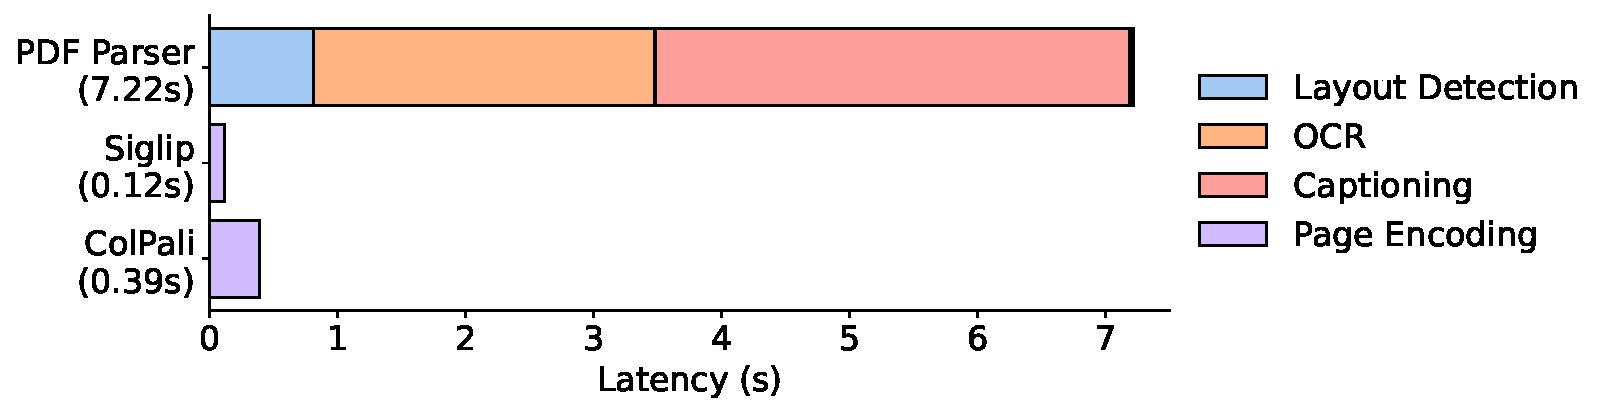
\includegraphics[width = 0.85\linewidth]{images/colpali_images/latency_comparison.pdf}
    \caption[Offline indexing latency comparison]{Offline document indexing with \textit{ColPali} is much simpler and faster compared to standard retrieval methods. The PDF Parser results are obtained following the \textit{Unstructured} settings with BGE-M3 detailed in \autoref{subsection:baseline_models}. All indexing speeds are averaged per-page latencies. More details in \autoref{paragraph:latency_app}}.
    \label{fig:latency-comparison}
\end{figure}




\section{Late interaction based Vision Retrieval}

% We propose adapting recent VLMs that have shown strong document understanding potential for multi-modal retrieval. 

% In this work, we aim to extract meaningful multi-vectorial representations of documents, relying solely on the image representation. Our proposed architecture design is presented in Figure 1.


\subsection{Architecture}
\label{subsection:colpali:architecture}


\textbf{Vision-Language Models.}
Encouraged by their strong document understanding capabilities, we propose adapting recent VLMs for retrieval. The key concept is to leverage the alignment between output embeddings of text and image tokens acquired during multi-modal fine-tuning. 
% We hypothesize that using the LLM text backbone to further encode the input image patches will integrate world-knowledge and reasoning capabilities that are key to understanding complex tables or charts. 
To this extent, we introduce \textit{ColPali}, a Paligemma-3B extension that is capable of generating ColBERT-style multi-vector representations of text and images (\autoref{fig:colpali_architecture}).
PaliGemma-3B is a strong candidate due to its small size, the many released checkpoints fine-tuned for different image resolutions and tasks, and the promising performances on various document understanding benchmarks. 
We add a projection layer to map each of the language model's output token embeddings (whether from text or image tokens)  to a vector space of reduced dimension $D = 128$ as used in the ColBERT paper \sidecite{khattab_colbert_2020} to keep lightweight bag-of-embedding representations.


\noindent\textbf{Late Interaction.}
% NOTE: archived because the R^D doesn't display properly.
% Let $q$ be the user query and $p$ a given document page. Let $\mathbf{E_q}_{(1:N_q)} = \left( \mathbf{E_q}^{(1)}, \ldots, \mathbf{E_q}^{(N_q)} \right) \in \left( \mathbb{R}^D \right)^{N_q}$ and $\mathbf{E_p}_{(1:N_p)} = \left( \mathbf{E_p}^{(1)}, \ldots, \mathbf{E_p}^{(N_p)} \right) \in \left( \mathbb{R}^D \right)^{N_p}$ their multi-vector representation in the common embedding space of dimension $D$.
Given query $q$ and document $d$, we denote as $\mathbf{E_q} \in \mathbb{R}^{{N_q} \times D}$ and $\mathbf{E_d} \in \mathbb{R}^{N_d \times D}$ their respective multi-vector representation in the common embedding space $\mathbb{R}^D$, where $N_q$ and $N_d$ are respectively the number of vectors in the query and in the document page embeddings. The late interaction operator, $\text{LI} \left( q, d \right)$, is the sum over all query vectors $\mathbf{E_{q}}^{(j)}$, of its maximum dot product $\langle \cdot | \cdot \rangle$ with each of the $N_d$ document embedding vectors $\mathbf{E_d}_{(1:N_d)}$.

\begin{equation}
    \text{LI} \left( q, d \right) = \sum_{i \in [|1, N_q|]} \max_{j \in [|1, N_d|]} \langle \mathbf{E_{q}}^{(i)} | \mathbf{E_{d}}^{(j)} \rangle
\label{eq:colbert_maxsim_score}
\end{equation}

% \ptitle{Contrastive batched loss: negative log of the softmax of the ratio of positive score to the negative scores}

\noindent\textbf{Contrastive Loss.}
The Late Interaction operation is fully differentiable, enabling backpropagation.
Let a batch $\left\{ q_k, d_k \right\}_{k \in [|1, b |]}$ composed of $b$ query-page pairs, where for all $k \in [|1, b|]$, the document page $d_k$ is the document corresponding to query $q_k$. 
% Thus, following the work of \citealt{sohn_improved_2016}, we can construct $b(b-1)$ negative pairs for this batch: the $\left\{ q_k, d_l \right\}_{k \neq l}$ (\textit{in-batch negatives}).
Following \sidecite{khattab_colbert_2020}, we define our in-batch contrastive loss $\mathcal{L}$ as the softmaxed cross-entropy of the positive scores $s_k^+ = \text{LI} \left( q_k, d_k \right)$ w.r.t. to the maximal in-batch negative scores $s_k^- = \max \limits_{l, l \neq k} \hspace{3mm} \text{LI} \left( q_k, d_l \right) $\sidenote{We reformulate the loss to leverage the numerically stable \texttt{softplus} function where $\texttt{softplus(x)} =  \log \left( 1 + \exp \left( x \right)\right)$}:

% \begin{equation}
%     \mathcal{L} = \frac{1}{b} \sum_{k=1}^{b} \texttt{softplus} \left( s_k^- - s_k^+ \right)
%     \label{equation:colpali_loss_final}
% \end{equation}



% NOTE: Full equation -> excluded because doesn't fit the column.
% \begin{equation}
%     \mathcal{L} = -\frac{1}{b} \sum_{k=1}^{b} \log \left[ \frac{\exp \left( s \left( q_k, p_k \right) \right)}{\exp \left( s \left( q_k, p_k \right) \right) + \exp \left( \max \limits_{l \in [|1, \ldots, b|] \atop l \neq k} \[ s \left( q_k, p_l \right) \] \right) } \right]
%     \label{equation:colpali_loss_full}
% \end{equation}

\begin{equation}
    \mathcal{L} = -\frac{1}{b} \sum_{k=1}^{b} \log \left[ \frac{\exp \left( s_k^+ \right)}{\exp \left( s_k^+ \right) + \exp \left( s_k^- \right)} \right] = \frac{1}{b} \sum_{k=1}^{b} \log \left( 1 + \exp \left( s_k^- - s_k^+ \right) \right)
    \label{equation:colpali_loss_full}
\end{equation}

% For all $k \in [|1, b|]$, let $s_k^+ = s(q_k, p_k)$ and $s_k^- = \max \limits_{l \in [|1, \ldots, b|] \atop l \neq k} \left( s(q_k, p_l) \right)$.



\subsection{Model training}

\noindent\textbf{Dataset.} Our training dataset of 118,695 query-page pairs is comprised of train sets of openly available academic datasets ($63\%$) and a synthetic dataset made up of pages from web-crawled PDF documents and augmented with VLM-generated (Claude-3 Sonnet) pseudo-questions ($37\%$). Dataset split details are given in \autoref{subsection:training_dataset}.
Our training set is fully English by design, enabling us to study zero-shot generalization to non-English languages\sidenote{Multilingual data is present in the pretraining corpus of the language model (Gemma-2B) and potentially occurs during PaliGemma-3B's multimodal training.}. We explicitly verify no multi-page PDF document is used both \textit{ViDoRe} and in the train set to prevent evaluation contamination. A validation set is created with $2\%$ of the samples to tune hyperparameters. We openly release the training dataset\sidenote{\url{https://huggingface.co/datasets/vidore/colpali_train_set}} for reproducibility and to encourage further research. 

\noindent\textbf{Parameters.} All models are trained for 1 epoch on the train set. Unless specified otherwise, we train models in \texttt{bfloat16} format, use low-rank adapters (LoRA, \sidecite{hu2021loralowrankadaptationlarge}) with $\alpha=32 $ and $r=32$ on the transformer layers from the language model, as well as the final randomly initialized projection layer, and use a \texttt{paged\_adamw\_8bit} optimizer. We train on an 8 GPU setup with data parallelism, a learning rate of $5e-5$ with linear decay with 2.5\% warmup steps, and a batch size of 32.

% Our reference model is ColPali with 1024 image patches, trained with memory tokens, a pairwise CE loss, a frozen vision component and an exclusively English training set.

\noindent\textbf{Query Augmentation.} As in \sidecite{khattab_colbert_2020}, we append 5 \texttt{<unused0>} tokens to the query tokens to serve as a soft, differentiable query expansion or re-weighting mechanism. 
%We do the same for the image patches, drawing inspiration from \sidecite{darcet_vision_2023}.

% We also explore the effect of adding the table and the figures to a naive baseline of only OCR. 

\section{Results}
\label{section:colpali:results}




\begin{table*}[ht]
    \centering
    
    \resizebox{\textwidth}{!}{%
    \begin{tabular}{ll@{\hskip 0.5em}l@{\hskip 0.5em}l@{\hskip 0.5em}l@{\hskip 0.5em}l@{\hskip 0.5em}l@{\hskip 0.5em}l@{\hskip 0.5em}l@{\hskip 0.5em}l@{\hskip 0.5em}l|@{\hskip 0.5em}l}

\toprule
 & \textbf{ArxivQ} & \textbf{DocQ} & \textbf{InfoQ} & \textbf{TabF} & \textbf{TATQ} & \textbf{Shift} & \textbf{AI} & \textbf{Energy} & \textbf{Gov.} & \textbf{Health.} & \textbf{Avg.} \\


 % Captioning$_{\tiny \texttt{e5-large}}$ & 30.9\textcolor{red!75!black}{\tiny $\downarrow$-4.2} & 24.0\textcolor{red!75!black}{\tiny $\downarrow$-5.8} & 62.3\textcolor{green!75!black}{\tiny $\uparrow$0.8} & 54.3\textcolor{green!75!black}{\tiny $\uparrow$29.3} & 37.6\textcolor{red!75!black}{\tiny $\downarrow$-11.3} & 44.0\textcolor{red!75!black}{\tiny $\downarrow$-3.0} & 76.0\textcolor{red!75!black}{\tiny $\downarrow$-3.0} & 71.0\textcolor{red!75!black}{\tiny $\downarrow$-5.0} & 70.0\textcolor{red!75!black}{\tiny $\downarrow$-5.0} & 72.0\textcolor{red!75!black}{\tiny $\downarrow$-9.0} \\



\midrule
    \multicolumn{0}{l}{\textbf{\texttt{Unstructured} \tiny text-only}}&&&&&&&&&&&\\
- BM25 & - & 34.1 & - & - & 44.0 & 59.6 & 90.4 & 78.3 & 78.8 & 82.6 &-\\
- BGE-M3 & - & 28.4\textcolor{red!75!black}{\tiny $\downarrow$5.7} & - & - & 36.1\textcolor{red!75!black}{\tiny $\downarrow$7.9} & 68.5\textcolor{green!75!black}{\tiny $\uparrow$8.9} & 88.4\textcolor{red!75!black}{\tiny $\downarrow$2.0} & 76.8\textcolor{red!75!black}{\tiny $\downarrow$1.5} & 77.7\textcolor{red!75!black}{\tiny $\downarrow$1.1} & 84.6\textcolor{green!75!black}{\tiny $\uparrow$2.0} & -\\
\\
\multicolumn{0}{l}{\textbf{\texttt{Unstructured} \tiny+ OCR}}&&&&&&&&&&&\\
- BM25 & 31.6 & 36.8 & 62.9 & 46.5 & 62.7 & 64.3 & 92.8 & 85.9 & 83.9 & 87.2 & 65.5\\
- BGE-M3 & 31.4\textcolor{red!75!black}{\tiny $\downarrow$0.2} & 25.7\textcolor{red!75!black}{\tiny $\downarrow$11.1} & 60.1\textcolor{red!75!black}{\tiny $\downarrow$2.8} & 70.8\textcolor{green!75!black}{\tiny $\uparrow$24.3} & 50.5\textcolor{red!75!black}{\tiny $\downarrow$12.2} & \textbf{73.2}\textcolor{green!75!black}{\tiny $\uparrow$8.9} & 90.2\textcolor{red!75!black}{\tiny $\downarrow$2.6} & 83.6\textcolor{red!75!black}{\tiny $\downarrow$2.3} & 84.9\textcolor{green!75!black}{\tiny $\uparrow$1.0} & 91.1\textcolor{green!75!black}{\tiny $\uparrow$3.9} & 66.1\textcolor{green!75!black}{\tiny $\uparrow$0.6}\\
\\
\multicolumn{0}{l}{\textbf{\texttt{Unstructured} \tiny+ Captioning}}&&&&&&&&&&&\\
- BM25 & 40.1 & 38.4 & 70.0 & 35.4 & 61.5 & 60.9 & 88.0 & 84.7 & 82.7 & 89.2 
& 65.1\\
- BGE-M3 & 35.7\textcolor{red!75!black}{\tiny $\downarrow$4.4} & 32.9\textcolor{red!75!black}{\tiny $\downarrow$5.4} & 71.9\textcolor{green!75!black}{\tiny $\uparrow$1.9} & 69.1\textcolor{green!75!black}{\tiny $\uparrow$33.7} & 43.8\textcolor{red!75!black}{\tiny $\downarrow$17.7} & 73.1\textcolor{green!75!black}{\tiny $\uparrow$12.2} & 88.8\textcolor{green!75!black}{\tiny $\uparrow$0.8} & 83.3\textcolor{red!75!black}{\tiny $\downarrow$1.4} & 80.4\textcolor{red!75!black}{\tiny $\downarrow$2.3} & 91.3\textcolor{green!75!black}{\tiny $\uparrow$2.1} & 67.0\textcolor{green!75!black}{\tiny $\uparrow$1.9}\\
    \midrule
    % \textbf{Multimodal emb.} &\\
    \multicolumn{0}{l}{\textbf{Contrastive VLMs}}&&&&&&&&&&&\\
    Jina-CLIP & 25.4 & 11.9 & 35.5 & 20.2 & 3.3 & 3.8 & 15.2 & 19.7 & 21.4 & 20.8 & 17.7 \\
    Nomic-vision & 17.1 & 10.7 & 30.1 & 16.3 & 2.7 & 1.1 & 12.9 & 10.9 & 11.4 & 15.7 & 12.9\\
    SigLIP \tiny(Vanilla)& 43.2 & 30.3 & 64.1 & 58.1 & 26.2 & 18.7 & 62.5 & 65.7 & 66.1 & 79.1 & 51.4 \\
\midrule
\multicolumn{0}{l}{\textbf{Ours}}&&&&&&&&&&&\\
SigLIP \tiny(Vanilla)& 43.2 & 30.3 & 64.1 & 58.1 & 26.2 & 18.7 & 62.5 & 65.7 & 66.1 & 79.1 & 51.4 \\
BiSigLIP \tiny (+fine-tuning) & 58.5\textcolor{green!75!black}{\tiny $\uparrow$15.3} & 32.9\textcolor{green!75!black}{\tiny $\uparrow$2.6} & 70.5\textcolor{green!75!black}{\tiny $\uparrow$6.4} & 62.7\textcolor{green!75!black}{\tiny $\uparrow$4.6} & 30.5\textcolor{green!75!black}{\tiny $\uparrow$4.3} & 26.5\textcolor{green!75!black}{\tiny $\uparrow$7.8} & 74.3\textcolor{green!75!black}{\tiny $\uparrow$11.8} & 73.7\textcolor{green!75!black}{\tiny $\uparrow$8.0} & 74.2\textcolor{green!75!black}{\tiny $\uparrow$8.1} & 82.3\textcolor{green!75!black}{\tiny $\uparrow$3.2} & 58.6\textcolor{green!75!black}{\tiny $\uparrow$7.2}\\

BiPali \tiny (+LLM) & 56.5\textcolor{red!75!black}{\tiny $\downarrow$-2.0} & 30.0\textcolor{red!75!black}{\tiny $\downarrow$-2.9} & 67.4\textcolor{red!75!black}{\tiny $\downarrow$-3.1} & 76.9\textcolor{green!75!black}{\tiny $\uparrow$14.2} & 33.4\textcolor{green!75!black}{\tiny $\uparrow$2.9} & 43.7\textcolor{green!75!black}{\tiny $\uparrow$17.2} & 71.2\textcolor{red!75!black}{\tiny $\downarrow$-3.1} & 61.9\textcolor{red!75!black}{\tiny $\downarrow$-11.7} & 73.8\textcolor{red!75!black}{\tiny $\downarrow$-0.4} & 73.6\textcolor{red!75!black}{\tiny $\downarrow$-8.8} & 58.8\textcolor{green!75!black}{\tiny $\uparrow$0.2}\\
\textit{ColPali} \tiny (+Late Inter.) & \textbf{79.1}\textcolor{green!75!black}{\tiny $\uparrow$22.6} & \textbf{54.4}\textcolor{green!75!black}{\tiny $\uparrow$24.5} & \textbf{81.8}\textcolor{green!75!black}{\tiny $\uparrow$14.4} & \textbf{83.9}\textcolor{green!75!black}{\tiny $\uparrow$7.0} & \textbf{65.8}\textcolor{green!75!black}{\tiny $\uparrow$32.4} & \textbf{73.2}\textcolor{green!75!black}{\tiny $\uparrow$29.5} & \textbf{96.2}\textcolor{green!75!black}{\tiny $\uparrow$25.0} & \textbf{91.0}\textcolor{green!75!black}{\tiny $\uparrow$29.1} & \textbf{92.7}\textcolor{green!75!black}{\tiny $\uparrow$18.9} & \textbf{94.4}\textcolor{green!75!black}{\tiny $\uparrow$20.8} & \textbf{81.3}\textcolor{green!75!black}{\tiny $\uparrow$22.5}\\

\bottomrule

\end{tabular}}


    \caption[Baseline and \textit{ViDoRe} evaluation]{\textbf{Comprehensive evaluation of baseline models and our proposed method on \textit{ViDoRe}.} Results are presented using nDCG@5 metrics, and illustrate the impact of different components. Text-only metrics are not computed for benchmarks with only visual elements.} 
    \label{table:colpali:results}
\end{table*}



\subsection{Performance (R1)}
\label{subsection:performace}

% We iteratively construct \textit{ColPali}, starting from an off-the-shelf SigLIP model (\autoref{table:results}).

We show performance is achieved iteratively through the combination of three factors; (1) a carefully crafted task-specific dataset, (2) pairing a pretrained LLM to a vision model to better leverage text semantics from the image, and (3) using multi-vector embeddings rather than a single vector representation to better capture the vast amount of visual information present in a document.
 
%\noindent\textbf{BiSigLIP: Improving a strong model.} SigLIP\sidenote{\url{https://huggingface.co/google/siglip-so400m-patch14-384}} is a strong vision-language bi-encoder model, pretrained on the English split of WebLI \sidecite{chen_pali-3_2023}, a corpus of billions of image-text pairs. We find that SigLIP largely outperforms both Jina CLIP and Nomic-vision on document retrieval tasks. Further fine-tuning the textual component of this model on our document-oriented dataset (BiSigLIP) yields clear improvements across the board, particularly on figure retrieval (ArxivQA) and table retrieval tasks (TabFQuAD).
\noindent\textbf{Fine-tuning a Vision Model on a document retrieval oriented dataset: \textit{BiSigLIP}.} SigLIP\sidenote{\url{https://huggingface.co/google/siglip-so400m-patch14-384}} is a strong vision-language bi-encoder producing single vector embeddings, and pretrained on billions of image-text pairs from the English split of WebLI \sidecite{chen_pali-3_2023}. Further fine-tuning the textual component of this model on our document-oriented dataset (BiSigLIP) yields clear improvements across the board, particularly on figure retrieval (ArxivQA) and table retrieval tasks (TabFQuAD).

% \noindent\textbf{BiPali: Pairing with a language model.} In the PaliGemma model architecture, SigLIP-generated patch embeddings are fed to a text language model to obtain LLM contextualized output patch embeddings.\sidenote{Note that the SigLIP model used in PaliGemma slightly differs in terms of number patches -  1024 patches for PaliGemma's vision encoder, and 729 for the standalone SigLIP model.} We average pool these representations to obtain a single dense vector, effectively creating a PaliGemma bi-encoder model (BiPali). After fine-tuning on the training dataset, we obtain a model that performs slightly worse in English than the tuned BiSigLIP variant. This can be explained by the fact that contrary to SigLIP, the original PaliGemma is not trained on contrastive matching tasks, but rather on next token prediction. Our contrastive fine-tuning phase on 119K images to transform PaliGemma into a bi-encoder is 5 orders of magnitude smaller than SigLIP's original contrastive training. However, we see notable improvements in French tasks, indicating that BiPali's LLM (Gemma 2B) helps multilingual text understanding. This is particularly notable as our training dataset does not contain non-English samples.

\noindent\textbf{Feeding image patches to a LLM: \textit{BiPali}.} In the PaliGemma model architecture, SigLIP-generated patch embeddings are fed to a text language model and we can obtain LLM contextualized output patch embeddings.\sidenote{Note that the SigLIP model used in PaliGemma slightly differs in terms of number patches -  1024 patches for PaliGemma's vision encoder, and 729 for the standalone SigLIP model.} This technique aligns the image token representations with the text token embeddings in the LLM's embeddings space, and augments the vision model embeddings with the language model's text understanding capabilities. We average pool these representations to obtain a single dense vector, effectively creating a PaliGemma bi-encoder model (BiPali). After fine-tuning on the training dataset, we obtain a model that performs slightly worse in English than the tuned BiSigLIP variant.\sidenote{This can be explained by the fact that contrary to SigLIP, the original PaliGemma is not trained on contrastive matching tasks, but rather on next token prediction. Our contrastive fine-tuning phase on 119K images to transform PaliGemma into a bi-encoder is 5 orders of magnitude smaller than SigLIP's original contrastive training.} However, we see notable improvements in French tasks, indicating that BiPali's LLM (Gemma 2B) helps multilingual text understanding. This is particularly notable as our training dataset does not contain non-English samples.

% \noindent\textbf{\textit{ColPali}: Adding Late Interaction.}
% One benefit of inputting image patch embeddings through a language model is that they are natively mapped to a latent space similar to textual input (query). This enables leveraging the ColBERT strategy to compute interactions between text tokens and image patches, which enables a step-change improvement in performance compared to BiPali. 
% Results in \autoref{table:results} show that our \textit{ColPali} model also largely outperforms the strong baselines based on \texttt{Unstructured} and captioning, as well as all evaluated text-image embedding models. The difference is particularly stark on the more visually complex benchmark tasks, such as InfographicVQA, ArxivQA, and TabFQuAD representing respectively infographics, figures, and tables. However, text-centric documents are also better retrieved by the \textit{ColPali} models across all evaluated domains and languages, making our approach the overall best-performing document-retrieval model.

\noindent\textbf{Leveraging Multi-Vector Embeddings through Late Interaction: \textit{ColPali}.}
One benefit of inputting image patch embeddings through a language model is that they are natively mapped to a latent space similar to the textual input (query). This enables leveraging the ColBERT strategy to construct one embedding per image patch token, and at inference compute all interactions between text tokens and image patches, resulting in a step-change improvement in performance compared to BiPali. 
Results in \autoref{table:colpali:results} show that our \textit{ColPali} model also largely outperforms the strong baselines based on \texttt{Unstructured} and captioning, as well as all evaluated text-image embedding models. The difference is particularly stark on the more visually complex benchmark tasks, such as InfographicVQA, ArxivQA, and TabFQuAD, respectively representing infographics, figures, and tables. However, text-centric documents are also better retrieved by the \textit{ColPali} models across all evaluated domains and languages, making our approach the overall best-performing document-retrieval model.

\noindent\textbf{Negative Results.} For extensiveness, we also train ColSigLIP, a late interaction variant of the BiSigLIP model but obtain abysmal performances. We attribute this to the large gaps w.r.t. SigLIP's pre-training, in which only a pooled latent representation is used in the contrastive loss, which does not optimize the representations of individual patch and token embeddings. Similarly, we train a BiSigLIP$_{PaliGemma}$ variant, in which we retrieve the image representations from the SigLIP model that has been further updated by PaliGemma fine-tuning, and use the text representations from PaliGemma's text model. After fine-tuning on our dataset, performance is severely inferior to SigLIP$_{Vanilla}$ which simply encodes with SigLIP's original text and vision components. This indicates a logical misalignment between SigLIP embeddings, and Gemma embeddings after PaliGemma training. We detail these results in \autoref{subection:additional_results}.

%Add training infomation out-of-domain
% \noindent\textbf{Language Modeling helps.} Compared to a standard contrastive vision-language model like SigLIP, further fine-tuned on the same dataset, we are interested in observing the performance improvement obtained by feeding SigLIP tokens into a text language model. We denote the standard SigLIP bi-encoder as BiSigLIP and the bi-encoder version of ColPali as BiPali. In both models, we average pool the representations of respectively the query tokens and the image tokens.\sidenote{We have tried variants such as keeping only the last token but mean pooling yields the best results.} We also baseline BiSigLIP, the BiSigLIP encoder that has been further pre-trained as part of the PaliGemma model to analyze whether continued training with a generative language modeling objective helps refine image embeddings. Our results show the clear improvements of BiPali over BiSigLIP, demonstrating that the language model brings refined semantic understanding capabilities.
% \noindent\textbf{Late Interaction helps.} Also interesting are the performance gains obtained through the late interaction retrieval scheme. We show that compared to the bi-encoder BiPali, ColPali shows vastly improved metric performance across the board. 
% \noindent\textbf{Zero-shot multilingualism.}
% Images are particularly good candidates for such a scheme thanks to their fixed size


\subsection{Latencies \& Memory Footprint}
\label{subsection:latency}
% Hugues

% TODO: https://arxiv.org/abs/2304.01982

\noindent \textbf{Online Querying. (R2)} Logically, querying latencies differ between \textit{ColPali} and a BGE-M3 embedding model. For BGE, encoding takes about $22$ ms for 15 tokens, while encoding a query with \textit{ColPali}'s language model takes about $30$ ms\sidenote{Computed for a batch size of $1$ (online), and averaged over 1000 queries. See \autoref{paragraph:latency_app}}. For smaller corpus sizes, computing the late interaction operation induces marginally small overheads ($\approx 1$ ms per 1000 pages in the corpus), and the cosine similarity computation between bi-encoder vectors is even faster. Optimized late interaction engines \sidecite{santhanam_plaid_2022, lee_rethinking_2023} enable to easily scale corpus sizes to millions of documents with reduced latency degradations.


\noindent\textbf{Offline Indexing. (R3)} 
Standard retrieval methods using bi-encoders represent each chunk as a single vector embedding, which is easy to store and fast to compute. However, processing a PDF to get the different chunks is the most time-consuming part (layout detection, OCR, chunking), and using captioning to handle multimodal data will only exacerbate this already lengthy process. On the other hand, \textit{ColPali} directly encodes pages from their image representation. Although the model is larger than standard retrieval encoders, skipping the preprocessing allows large speedups at indexing\sidenote{Measures a NVIDIA L4 GPU, averaged on 100 pages, with a batch size of 4 pages for \textit{ColPali} and 8 text chunks for Bi-Encoders. On average, a page is divided into 2.1 chunks. See \autoref{paragraph:latency_app}.} (\autoref{fig:latency-comparison}). As pages are embedded end-to-end in single forward pass, the VRAM usage depends exclusively on the sequence length (number of patches per image) which is fixed as well, enabling efficient batching strategies to fully leverage hardware acceleration. ColPali also benefits from most LLM efficiency improvements introduced in the ecosystem such as Flash Attention \sidecite{dao2023flashattention2fasterattentionbetter}.

\noindent\textbf{Storage Footprint.} Our method requires storing a vector per image patch, along with 6 extra text tokens ``Describe the image" concatenated to image patches. We project each PaliGemma vector to a lower dimensional space ($D=128$) to maximize efficiency, leading to a memory footprint of $257.5$ KB per page (\autoref{subsection:embedding_size}). Importantly, the memory footprint of the naive ColBERT indexing strategy can be drastically improved through compression and clustering mechanisms \sidecite{santhanam_plaid_2022, clavie_reducing_2024}.

\noindent\textbf{Token pooling.}
% Multi-vector embeddings scale linearly in size with respect to the number of tokens, inducing longer indexing and search time. 
Token pooling \sidecite{clavie_reducing_2024} is a CRUDE-compliant method (document addition/deletion-friendly) that aims amountto reduce the amount of multi-vector embeddings. For ColPali, many image patches share redundant information, e.g. white background patches. By pooling these patches together, we can reduce the amount of embeddings while retaining most information. Retrieval performance with hierarchical mean token pooling on image embeddings is shown in \autoref{fig:combined_figures} (left).
With a pool factor of 3, the total number of vectors is reduced by $66.7\%$ while $97.8\%$ of the original performance is maintained. We note that the Shift dataset—composed of the most text-dense documents—is a clear outlier, showcasing more information dense documents contain less redundant patches and may be prone to worse performance degradation with such pooling techniques.

\subsection{Interpretability}
\label{subsection:similarity_maps}

% \begin{figure}
% \centering
% % \includegraphics[width=0.5\linewidth]{images/colpali_images/similarity_maps/similarity_map_energy.png} 
% 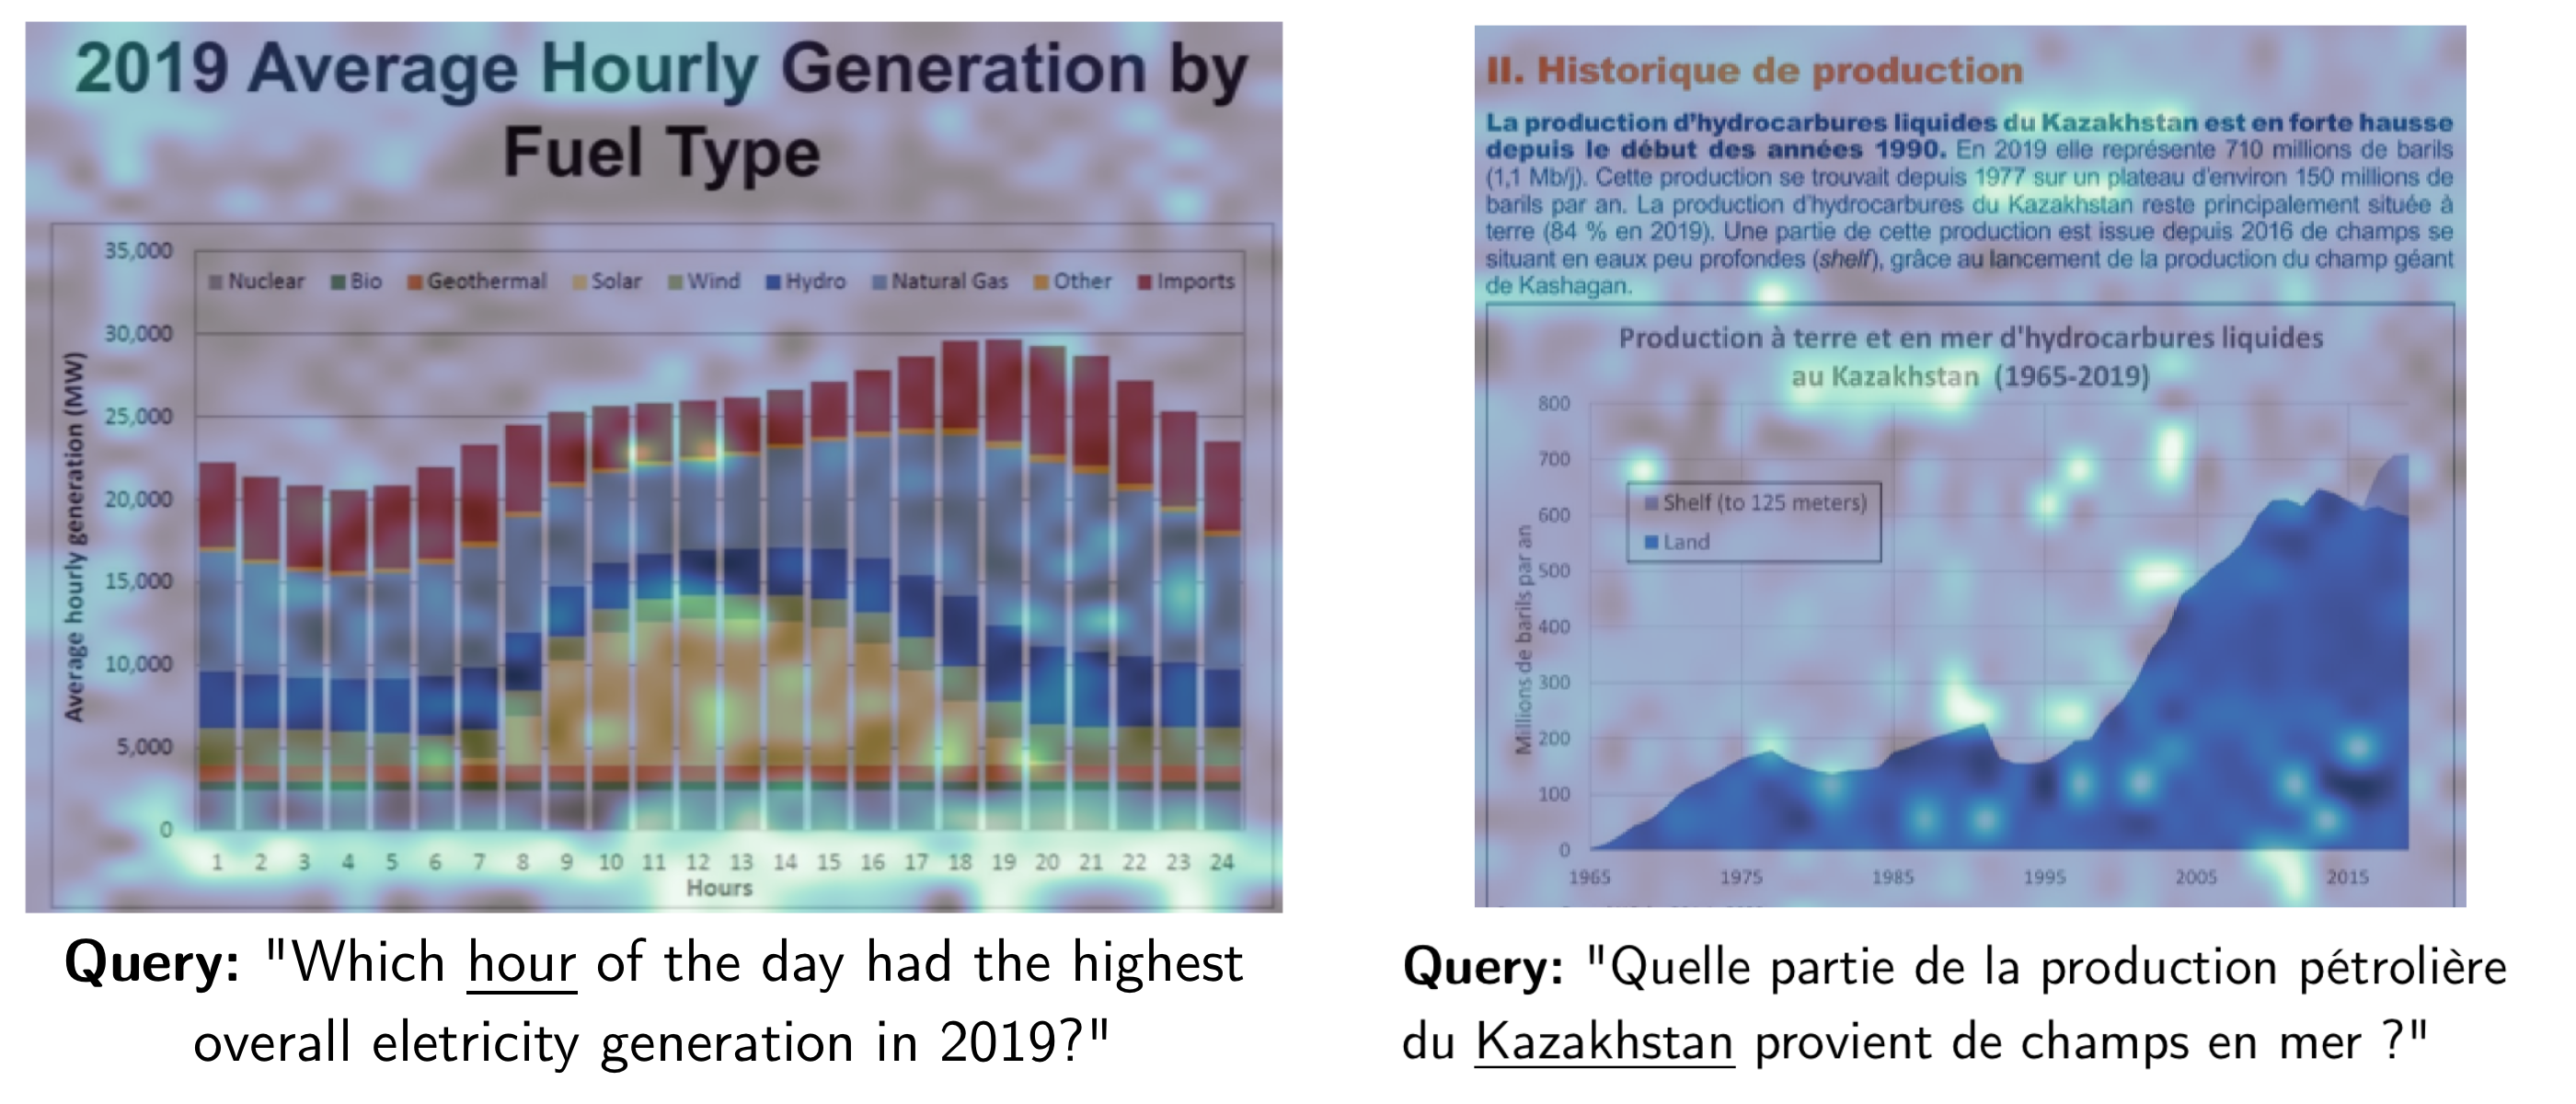
\includegraphics[width = 1\linewidth]{images/colpali_images/similarity_maps/similarity_maps.png} 
%     \caption{For each term in a user query, \textit{ColPali} identifies the most relevant document image patches (highlighted zones) and computes a query-to-page matching score. We can then swiftly retrieve the most relevant documents from a large pre-indexed corpus.}
% \label{fig:similarity_maps}
% \end{figure}


\begin{figure}
\centering
\begin{minipage}{.5\textwidth}
  \centering
  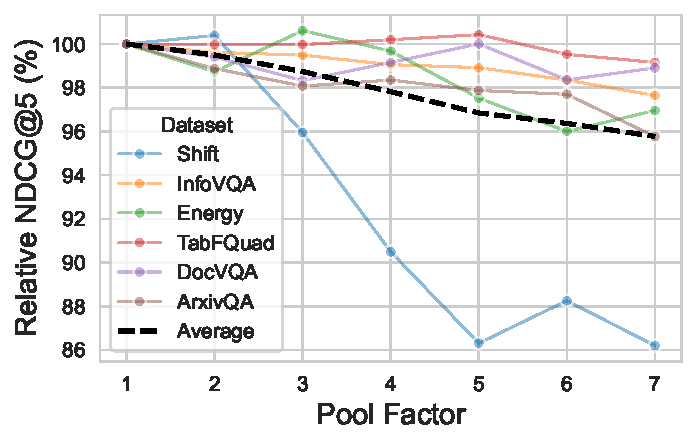
\includegraphics[width=1\linewidth]{images/colpali_images/token_pooling_ndcg.pdf}
\end{minipage}%
\begin{minipage}{.45\textwidth}
  \centering
  \includegraphics[width=0.9\linewidth]{images/colpali_images/similarity_map_energy.png}
\end{minipage}
\caption[Token pooling and interpretability]{(Left: \textbf{Token Pooling}) Relative performance degradation when reducing the number of stored embeddings per document. (Right: \textbf{Interpretability}) For each term in a user query, \textit{ColPali} identifies the most relevant document image patches (highlighted zones) and computes a query-to-page matching score.}
\label{fig:combined_figures}
\end{figure}

% \begin{figure}
% \centering
% \begin{minipage}{.45\textwidth}
%   \centering
%   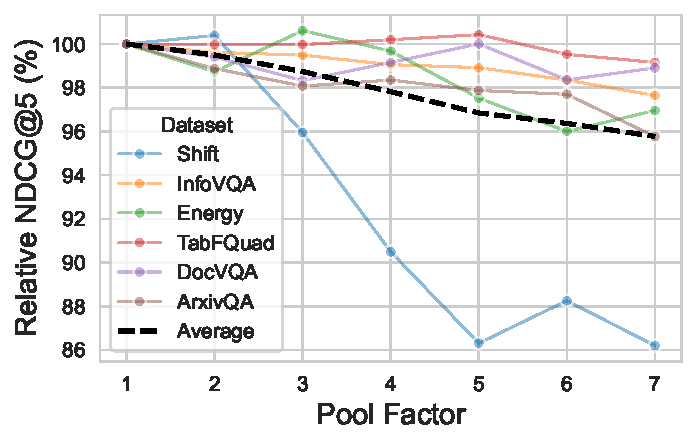
\includegraphics[width=1\linewidth]{images/colpali_images/token_pooling_ndcg.pdf}
%   \captionof{figure}{Relative performance degradation for token pooling on image embeddings generated by \textit{ColPali}.}
%   \label{fig:token-pooling}
% \end{minipage}
% \begin{minipage}{.45\textwidth}
%   \centering
%   \includegraphics[width=0.9\linewidth]{images/colpali_images/similarity_map_energy.png}
%   \captionof{figure}{For each term in a user query, \textit{ColPali} identifies the most relevant document image patches (highlighted zones) and computes a query-to-page matching score.}
%   \label{fig:similarity_maps}
% \end{minipage}%
% \end{figure}

% When we feed an image to ColPali, each image patch is mapped to a vector. Thus, the output is a sequence of $n_{\text{patch}}$ vectors. Because of the ViT positional embeddings and of the generative nature of the pre-trained LLM backbone in ColPali, we believe still have the notion of the image patch structure. Thus, we have mapped the output ColPali representation of the image to a $[0, 1]^{n_{\text{patch}}^2}$ matrix to visualize the per-patch similarity scores with a give query token. This is epitomized in \autoref{fig:similarity_map_hourly}.

%ColPali outputs a 128-dimensional vector for every input image patch (1024), which is used for late interaction matching.\


By superimposing the late interaction heatmap on top of the original image, we can visualize the most salient image patches with respect to each term of the query, yielding interpretable insights into model focus zones. As epitomized in \autoref{fig:combined_figures} (right), we observe \textit{ColPali} exhibits strong OCR capabilities as both the words \textit{``hourly"} and \textit{``hours"} present a high similarity score with the query token \texttt{<\_hour>}. We also note particular focus on other non-trivial image features such as the x-axis representing hours being salient. Other visualization examples are shown in \autoref{section:more_similarity_maps}.

% By superimposing the late interaction heatmap on top of the original image, we can visualize the most salient image patches with respect to each term of the query, yielding interpretable insights into model focus zones. In the first figure in \autoref{fig:similarity_maps}, we observe \textit{ColPali} exhibits strong OCR capabilities as both the words \textit{"hourly"} and \textit{"hours"} present a high similarity score with the query token \texttt{<\_hour>}. We also note particular focus on other non-trivial image features such as the x-axis representing hours being salient.

% Other visualization examples with similar trends of the model transcending pure OCR are shown in \autoref{section:more_similarity_maps}.

% Both similarity maps present a few white patches with high similarity scores. This behavior might first seem surprising as the white patches should not carry a meaningful signal from the original images. We believe the vectors associated with these patches share a similar role with the ViT registers \sidecite{darcet_vision_2023}, i.e.\ these patches were repurposed for internal computations and stored the global information from the whole image.


\section{Ablation study}
\label{section:ablation_study}

We run various ablations to better understand the mechanisms at play. By default, result deltas reported below refer to nDCG@5 values averaged over all ViDoRe tasks.  Detailed results in \ref{subection:model_variants}.

%\subsection{Is it better to increase model size or the number of patches ?}

%\noindent\textbf{Number of patches.} 
\noindent\textbf{Tradeoffs between model size and the number of image patches.} We train a variant of PaliGemma with half the number of image patches (512). % The number of tokens is directly linked to the resolution of the embedded image patches.
While we observe a clear performance degradation with respects to to the 1024-patch \textit{ColPali} model ($-24.8$ nDCG@5), memory usage is much lower.
%\sidenote{Yet another PaliGemma variant exists with 2048 patches, but the large memory requirements make this model impractical to train contrastitively and to run inference with.}
%\noindent\textbf{Language Model size.} 
As an alternative to PaliGemma, we train Idefics2-8B \sidecite{laurencon_what_2024}, a VLM with a similar architecture and based on a Mistral-7B \sidecite{jiang_mistral_2023} language backbone and a SigLIP vision encoder paired with a perceiver resampler. The most notable differences with PaliGemma lie in the size of the language model (2B and 7B resp.) and the number of image patches (between 512 and 2048 for PaliGemma, and 64 post-resampling for Idefics2\sidenote{With the option of adding 4 sub-image crops of 64 tokens each to the sequence, for a total of 320 tokens}). Our results suggest better language models enable more efficient representations of image embeddings - ColIdefics2 with 64 patches largely outperforms out \textit{ColPali} with 512 patches (+20.1 nDCG@5). However ColIdefics2 (64) remains less accurate than ColPali (1024) ($-4.7$ nDCG@5) while being about twice as slow in terms of training and inference latency.
%
%\noindent\textbf{Tradeoffs.} 
% Scaling the number of patches of the smaller \textit{ColPali} model from 512 to 1024, enables largely surpassing the 60-patch ColIdefics2 while being about twice as fast in terms of training and inference latency. 
These results suggest there are \textit{tradeoffs} between performance (R1), latencies during online querying (R2) and offline indexation phases (R3), and index memory size.

% \vspace{0.5cm}
\noindent\textbf{Unfreezing the vision component.} We train a \textit{ColPali} variant by also backpropagating through and updating the vision encoder and the projection layer. This leads to a slight performance degradation ($-0.7$ nDCG@5). These conclusions may change with larger scales of training data.

% \subsection{Do "query augmentation" tokens help ?}
% \vspace{0.2cm}
\noindent\textbf{Impact of ``query augmentation" tokens.} In ColBERT, special tokens are concatenated to the input query to serve as soft query augmentation buffers. Training without these tokens, we observe no significant performance difference in the English benchmarks. However, performance on the French tasks seems to improve ($+9.8$ nDCG@G on Shift, $+6.3$ nDCG@5 on TabFQuAD, \autoref{table:negative_results}).
% \sidecite{mckinzie_mm1_2024,bordes_introduction_2024,li_llava-next_2024}


% \subsection{Pairwise Cross-Entropy (CE) Loss}
% \vspace{0.2cm}
\noindent\textbf{Impact of the Pairwise CE loss.} Training with an in-batch negative contrastive loss, instead of the pairwise CE loss that only considers the hardest negative sample, leads to a slight performance degradation ($-1.6$ nDCG@5) on the aggregated benchmark.

% \vspace{0.2cm}
\noindent\textbf{Adapting models to new tasks.} Contrary to more complex multi-step retrieval pipelines, \textit{ColPali} can be trained end-to-end, directly optimizing the downstream retrieval task which greatly facilitates fine-tuning to boost performance on specialized domains, multilingual retrieval, or specific visual elements the model struggles with. To demonstrate, we add 1552 samples representing French tables and associated queries to the training set. This represents the only French data in the training set, with all other examples being kept unchanged. We see clear nDCG@5 improvements ($+2.6$) and even starker Recall@1 gains ($+5$) on the TabFQuAD benchmark, with no performance degradation on the rest of the benchmark tasks ($+0.4$ nDCG@5 overall).

\noindent\textbf{Better VLMs lead to better visual retrievers.} As improved VLMs are released, it is interesting to observe if improved performances on generative tasks translate once these models are adapted for image retrieval tasks through ColPali training strategies. We train the recently released Qwen2-VL 2B \sidecite{wang2024qwen2vlenhancingvisionlanguagemodels}, a SOTA 2 billion parameter generative VLM, with the same data and training strategy, obtaining ColQwen2-VL. To approximately match ColPali's memory requirements, we limit the number of image patches to 768, slightly less than ColPali's 1024 patches. We observe clear performance improvements of $+5.3$ nDCG@5 values over ColPali showcasing clear performance correlations between generative benchmarks performance and retrieving metrics.

\noindent\textbf{Out-of-domain generalization.} Some of the datasets in the ViDoRe benchmark have train sets, which we have integrated within the ColPali train set (eg. academic tasks). This is standard in embedding models \sidecite{wang2024improvingtextembeddingslarge, lee2024nvembedimprovedtechniquestraining}, and while ColPali also exhibits strong performance on tasks in which this is not the case (French data is never seen by the model during training for instance), it remains interesting to evaluate model performance when training is done on a fully disjoint data distribution. We train a ColPali variant solely using the recent DocMatix dataset \sidecite{laurençon2024building}, a large scale, synthetically annotated visual document question answering dataset, which we subsample to obtain a comparably-sized train set. Results on ViDoRe show the performance drop is minor ($-2.2$ nDCG@5), still outperforming the closest baseline method by over 12 points. These results showcase
ColPali generalizes well outside of its training distribution, and demonstrate that our results are not unreasonably boosted with respect to baselines (BGE-M3) that cannot be fine-tuned on the same data\sidenote{To train with data resembling the one BGE-M3 models would see at inference time would require running complex extraction pipelines for the more than 100K documents in the training set, notably relying on external proprietary captioning models which is both too costly and lengthy. This is not needed to train vision-based models.} 
%In practice, these models are most often used off-the-shelf without further fine-tuning in the majority of use cases.}

\section{Conclusions}
\label{section:colpali:conclusions_and_future_work}

In this work, we introduced the Visual Document Retrieval Benchmark (\textit{ViDoRe}), which evaluates document retrieval systems in realistic settings involving visually complex documents. We demonstrated that current retrieval pipelines and contrastive vision-language models struggle to efficiently exploit visual information embedded in documents, leading to suboptimal performance. To address this, we presented \textit{ColPali}, a novel retrieval method that leverages Vision-Language Models to create high-quality, multi-vector embeddings purely from visual document features. \textit{ColPali} largely outperforms the best existing document retrieval methods while enabling faster corpus indexing times and maintaining low querying latencies, thus circumventing many pain points of modern document retrieval applications. We hope to drive industrial adoption, and to encourage future work by publicly releasing the \textit{ViDoRe} benchmark, the data, the codebase, and all models and baselines from our work.

% hese results demonstrate the potential and the many benefits of this novel Retrieval in Vision Space concept, which could significantly alter the way document retrieval is approached in the industry moving forward. 

% Future work
% Image patch embeddings 
\noindent\textbf{Future Work.} 
% Further performance gains could be obtained by exploring sub-image decomposition \sidecite{liu_improved_2023}, optimal image patch resampling strategies \sidecite{laurencon_what_2024}, or hard-negative mining. 
%as well as training with larger batch size, 
% Next, we want to reduce the time and space footprint of our method using PLAID \sidecite{santhanam_plaid_2022} and XTR \sidecite{lee_rethinking_2023}. 
Beyond performance improvements that could be obtained through better data, backbone models or training strategies, our vision at term is to combine visual retrieval systems and visually grounded query answering to create end-to-end RAG systems that purely function from image features. This idea is supported by concurrent work \sidecite{ma2024mmlongbenchdocbenchmarkinglongcontextdocument} showcasing the strong promises of VLMs for visual QA, and may eventually become a new industrial standard for document processing. In this line of work, reliability is key, and confidence estimation techniques for Information Retrieval methods could become central to implement abstention mechanisms \sidecite{gisserotboukhlef2024trustworthyrerankingsimpleeffective}, and are particularly interesting given the information rich multi-vector scoring mechanisms of late interaction systems.
Expanding benchmarking efforts to cover more languages, modalities, and tasks is also a crucial future research direction \sidecite{jiang2024vlm2vectrainingvisionlanguagemodels}.
 
% , without having to reuse the original image.

% Similarly, as in GritLM, we could also envision a model that is performant both for retrieval and generative modeling.


% Mention it'd be great to test the two-stage e2e top-k retrieval from COlBERT's paper section 3.6

% Experiment aspect-preserving ViT grid = experiment any resolution
% \sidecite{dehghani_patch_2023}


% % Experiment sub-image decomposition
% Sub-image decomposition \sidecite{liu_improved_2023}
% Super sub-image decomposition \sidecite{li_llava-next_2024}

% % Add registers in the ViT
% Registers in the ViT \sidecite{darcet_vision_2023}


% % Experiment w/ LLM-as-encoders
% Try the better LLM fine-tuning with masking etc..
% \sidecite{behnamghader_llm2vec_2024}


% % Analyze the impact of resolution
% \sidecite{dou_empirical_2021}
% \sidecite{mckinzie_mm1_2024}

% Hard negative mining

% Recycle the model for different use cases (multi-adapters)
% GritLM
% webpages


% \section*{Limitations}
% \label{section:limitations}

% \noindent\textbf{Focus.} In this work, we evaluate models on document retrieval tasks, covering several modalities (figures, text, tables, infographics). We however primarily focus on PDF-type documents, and evaluating systems on image retrieval with documents stemming from web page screenshots or hand-written documents might be an interesting generalization. We also focus on high-resource languages (English and French) and although we have shown the capacity of the \textit{ColPali} model to generalize to languages outside of its fine-tuning set, it is unclear how the model would perform on languages that are not as represented in the model's language backbone. Finally, our setup assumes relevant documents exist, but abstention methods for Information Retrieval systems might be interesting to explore in more practical settings in which confidence estimation might be important \sidecite{gisserotboukhlef2024trustworthyrerankingsimpleeffective}.

% % memory requirementd --> deployment difficulty
% \noindent\textbf{Support.} This work relies on multi-vector retrieving derived from the ColBERT late interaction mechanism. Although some vector databases support late interaction engines\sidenote{\href{https://vespa.ai/}{Vespa Engine}, \href{https://github.com/bclavie/RAGatouille}{RAGatouille}, \href{https://github.com/qdrant/qdrant}{QDrant}, \href{https://github.com/stanford-futuredata/colbert}{colbert.ai}}, many widely used vector retrieval frameworks do not propose native multi-vector support, and some engineering infrastructure efforts may be required to adapt them to work with \textit{ColPali} (or ColBERT) models. 

% \noindent\textbf{Data.} In the creation of \textit{ViDoRe}, we partially rely on synthetic query generation based on a commercial large language model, which may induce some amount of bias in the generated queries. To compensate for this, we have iterated on the prompting strategy and given real query examples to the models to help ground generation in realistic settings. We have further manually verified all synthetic queries through a lengthy process to validate their relevance and their quality. Our benchmark also includes many benchmark tasks with no synthetic data, and result trends observed between all tasks are correlated, further confirming the coherence of our benchmark design.



% \section*{Ethics Statement}

% \noindent\textbf{Carbon Footprint.} Our work fully leverages prior pretrained models and training is not particularly compute-intensive. Furthermore, we rely on low-rank adapters to further reduce the computational resources needed, both during training and for storage. Overall, a training run represents about 40 hours of Mi250x AMD GPUs. Our experiments, in total, represent 1405 Mi250x GPU hours from highly efficient compute clusters running on low-carbon nuclear energy, representing a total of around 15kg CO2 eq.

% \noindent\textbf{Impact.} We believe our work could have a strong impact on improving industrial document retrieval systems. Our method is efficient, performs well, and the additional support towards visually rich information from documents could go a long way in unlocking knowledge sources previously difficult to index or query.

\section*{Reproducibility Statement}

For transparency, reproducibility and to foster future work, we release our training data, model checkpoints (adapters), entire codebase, and complete evaluation benchmark under MIT licenses as detailed in the main paper. We also host a public \textit{ViDoRe} leaderboard\sidenote{\url{https://huggingface.co/spaces/vidore/vidore-leaderboard}} to foster concurrent work in the space. The supplementary material further details training configurations for our models (also specified in HuggingFace model repositories), and dives into the process we used to generate synthetic data, how latency computations are performed, as well as provides further detailed evaluation results.



\section*{Acknowledgements}

This work is partially supported by Illuin Technology, and by a grant from ANRT France. This work was performed using HPC resources from the CINES ADASTRA through Grant 2024-AD011015443 and from IDRIS with grant 2024-AD011015724R1.
We extend our warm thanks to Jonathan Dong, Caio Corro, Victor Pellegrain and Ender Konukoglu for their valuable feedback on the paper.

% \setchapterpreamble[u]{\margintoc}
\chapter{ViDoRe V3: A Comprehensive Evaluation of Retrieval Augmented Generation in Complex Real-World Scenarios}


\begin{kaobox}[frametitle=Paper Abstract]
Retrieval-Augmented Generation (RAG) pipelines must address challenges beyond simple single-document retrieval, such as interpreting visual elements (tables, charts, images), synthesizing information across documents, and providing accurate source grounding. Existing benchmarks fail to capture this complexity, often focusing on textual data, single-document comprehension, or evaluating retrieval and generation in isolation. We introduce \textbf{\vidorev}, a comprehensive multimodal RAG benchmark featuring multi-type queries over visually rich document corpora. It covers 10 datasets across diverse professional domains, comprising ~26,000 document pages paired with 3,099 human-verified queries, each available in 6 languages. Through 12,000 hours of human annotation effort, we provide high-quality annotations for retrieval relevance, bounding box localization, and verified reference answers. Our evaluation of state-of-the-art RAG pipelines reveals that visual retrievers outperform textual ones, late-interaction models and textual reranking substantially improve performance, and hybrid or purely visual contexts enhance answer generation quality. However, current models still struggle with non-textual elements, open-ended queries, and fine-grained visual grounding. To encourage progress in addressing these challenges, the benchmark is released under a commercially permissive license.

\end{kaobox}

\section{Introduction}

\begin{figure*}[h]
    \centering
    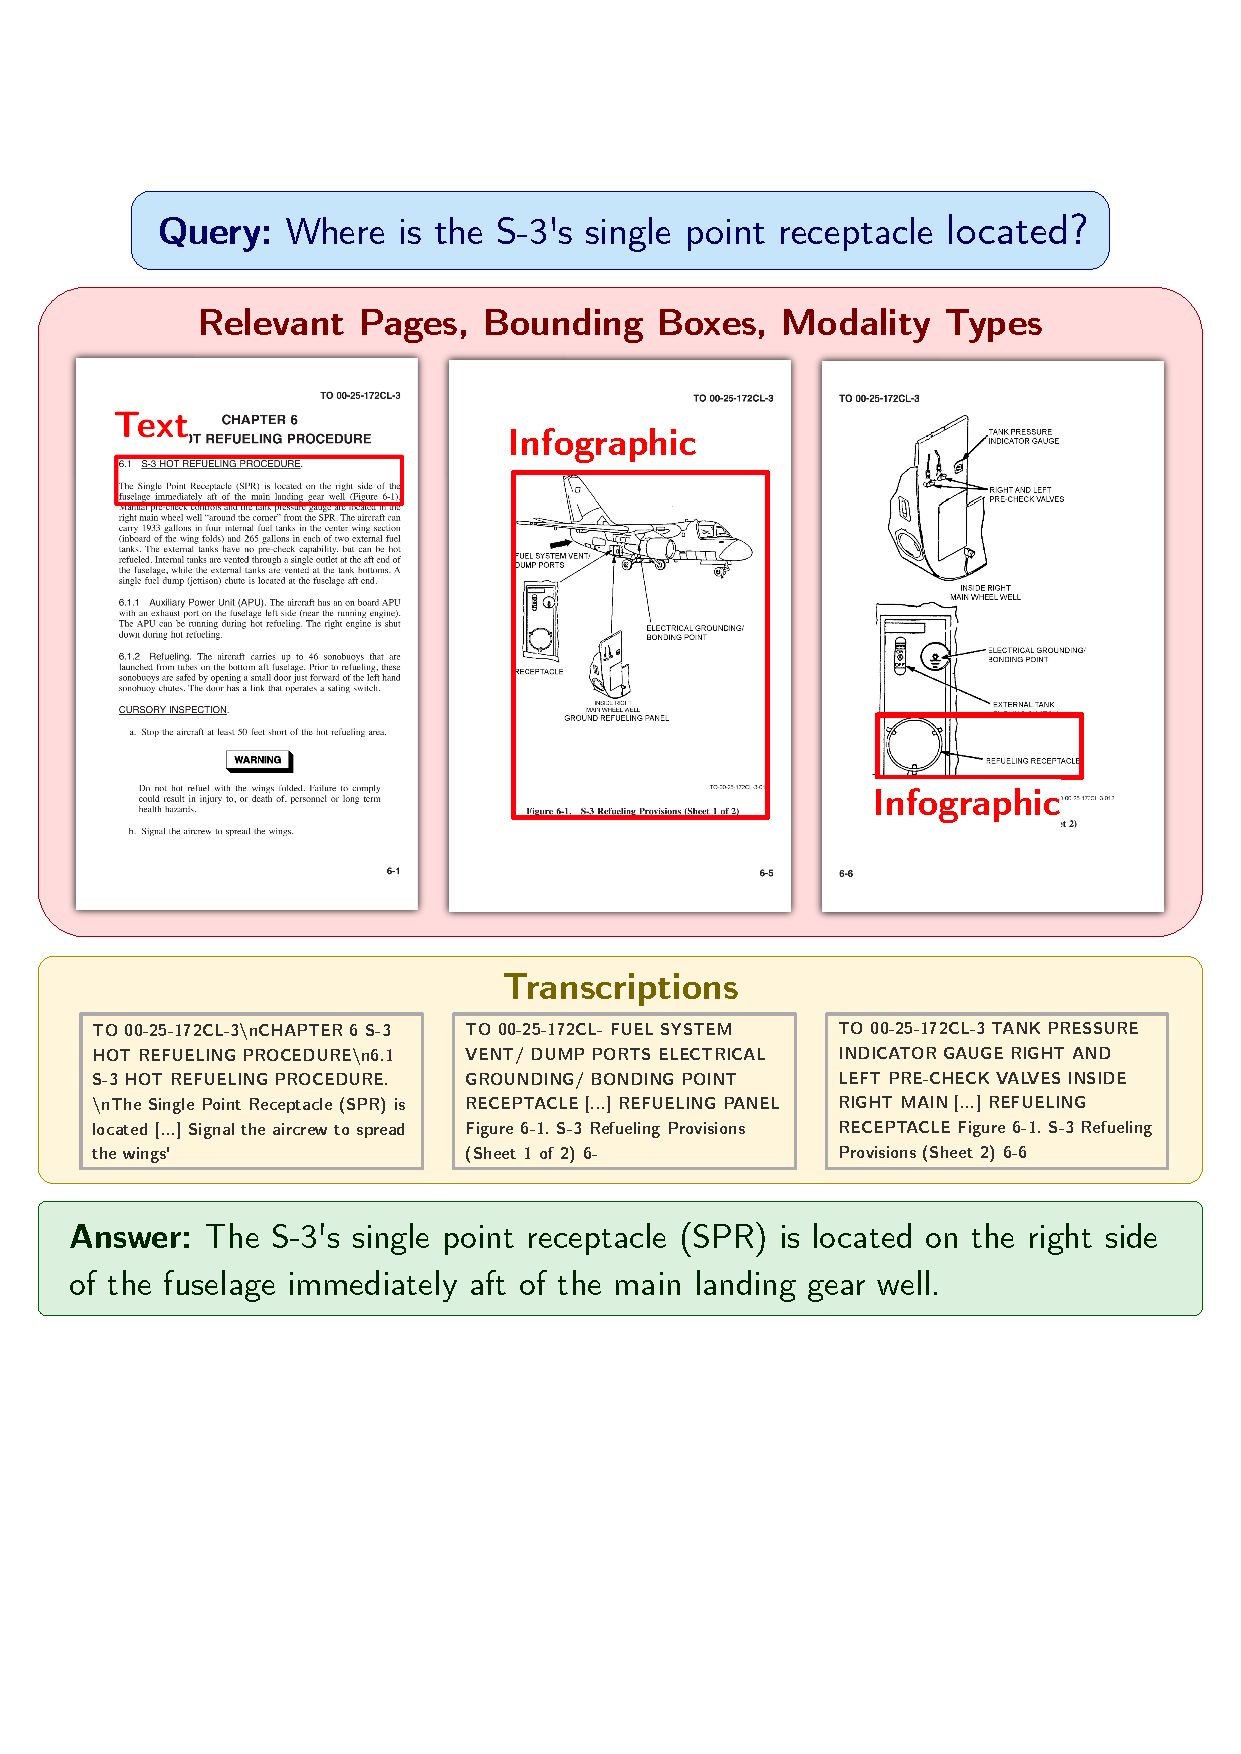
\includegraphics[trim={2cm 6.5cm 2cm 3.5cm}, clip, width=0.9\textwidth]{images/vidorev3_images/vidore_sample.pdf}
    \caption{\textbf{ViDoRe V3 sample.} Each query is annotated with the relevant pages, a document-grounded answer, bounding boxes localizing supporting evidence and modality labels for each bounding box. Documents are provided in image, text and PDF formats.} % TODO: clean this caption
    \label{fig:sample}
\end{figure*}

% In these settings, accurate information retrieval offers the highest operational value yet faces the most unstructured, heterogeneous data. That is why, real-world pipelines must tackle challenges that extend beyond single-document textual retrieval.

Retrieval-Augmented Generation (RAG) \sidecite{lewis2021retrievalaugmentedgenerationknowledgeintensivenlp} has become the dominant paradigm for knowledge-intensive NLP tasks \sidecite{gao2024retrievalaugmentedgenerationlargelanguage, fan2024surveyragmeetingllms}. Yet practical deployments introduce complexities that academic benchmarks often overlook when focusing on single-document textual retrieval. First, documents encode critical information in visual elements such as tables, charts, and images designed for human interpretation, which text-only pipelines often ignore \sidecite{abootorabi2025askmodalitycomprehensivesurvey, cho2024m3docragmultimodalretrievalneed}. Second, user queries often require open-ended synthesis, comparison, and reasoning over scattered information, not simple factoid lookup \sidecite{tang2024multihopragbenchmarkingretrievalaugmentedgeneration, conti2025contextgoldgoldpassage, thakur2025freshstackbuildingrealisticbenchmarks}. Third, trustworthy systems must ground responses to specific source locations (e.g., bounding boxes), to mitigate hallucinations \sidecite{gao2023enablinglargelanguagemodels, ma2024visaretrievalaugmentedgeneration}.

Existing benchmarks leave these requirements only partially addressed. Early Visual Document Understanding (VDU) benchmarks focus on single-page comprehension, ignoring the complexity of large document corpora \sidecite{mathew_docvqa_2020}. Recent retrieval-centric benchmarks do not evaluate generation quality and grounding \sidecite{faysse2025colpaliefficientdocumentretrieval,günther2025jinaembeddingsv4universalembeddingsmultimodal}. Some multimodal datasets attempt to bridge this gap but rely on extractive, short-answer tasks that fail to exercise complex reasoning \sidecite{cho2024m3docrag}, or lack multilingual diversity and fine-grained visual grounding \sidecite{peng2025unidocbenchunifiedbenchmarkdocumentcentric}.

\begin{figure*}[t!]
    \centering
    % \includegraphics[trim={0cm 2cm 0cm 2cm}, clip, width=\textwidth]{images/vidorev3_images/test-vidore-v0.png}
    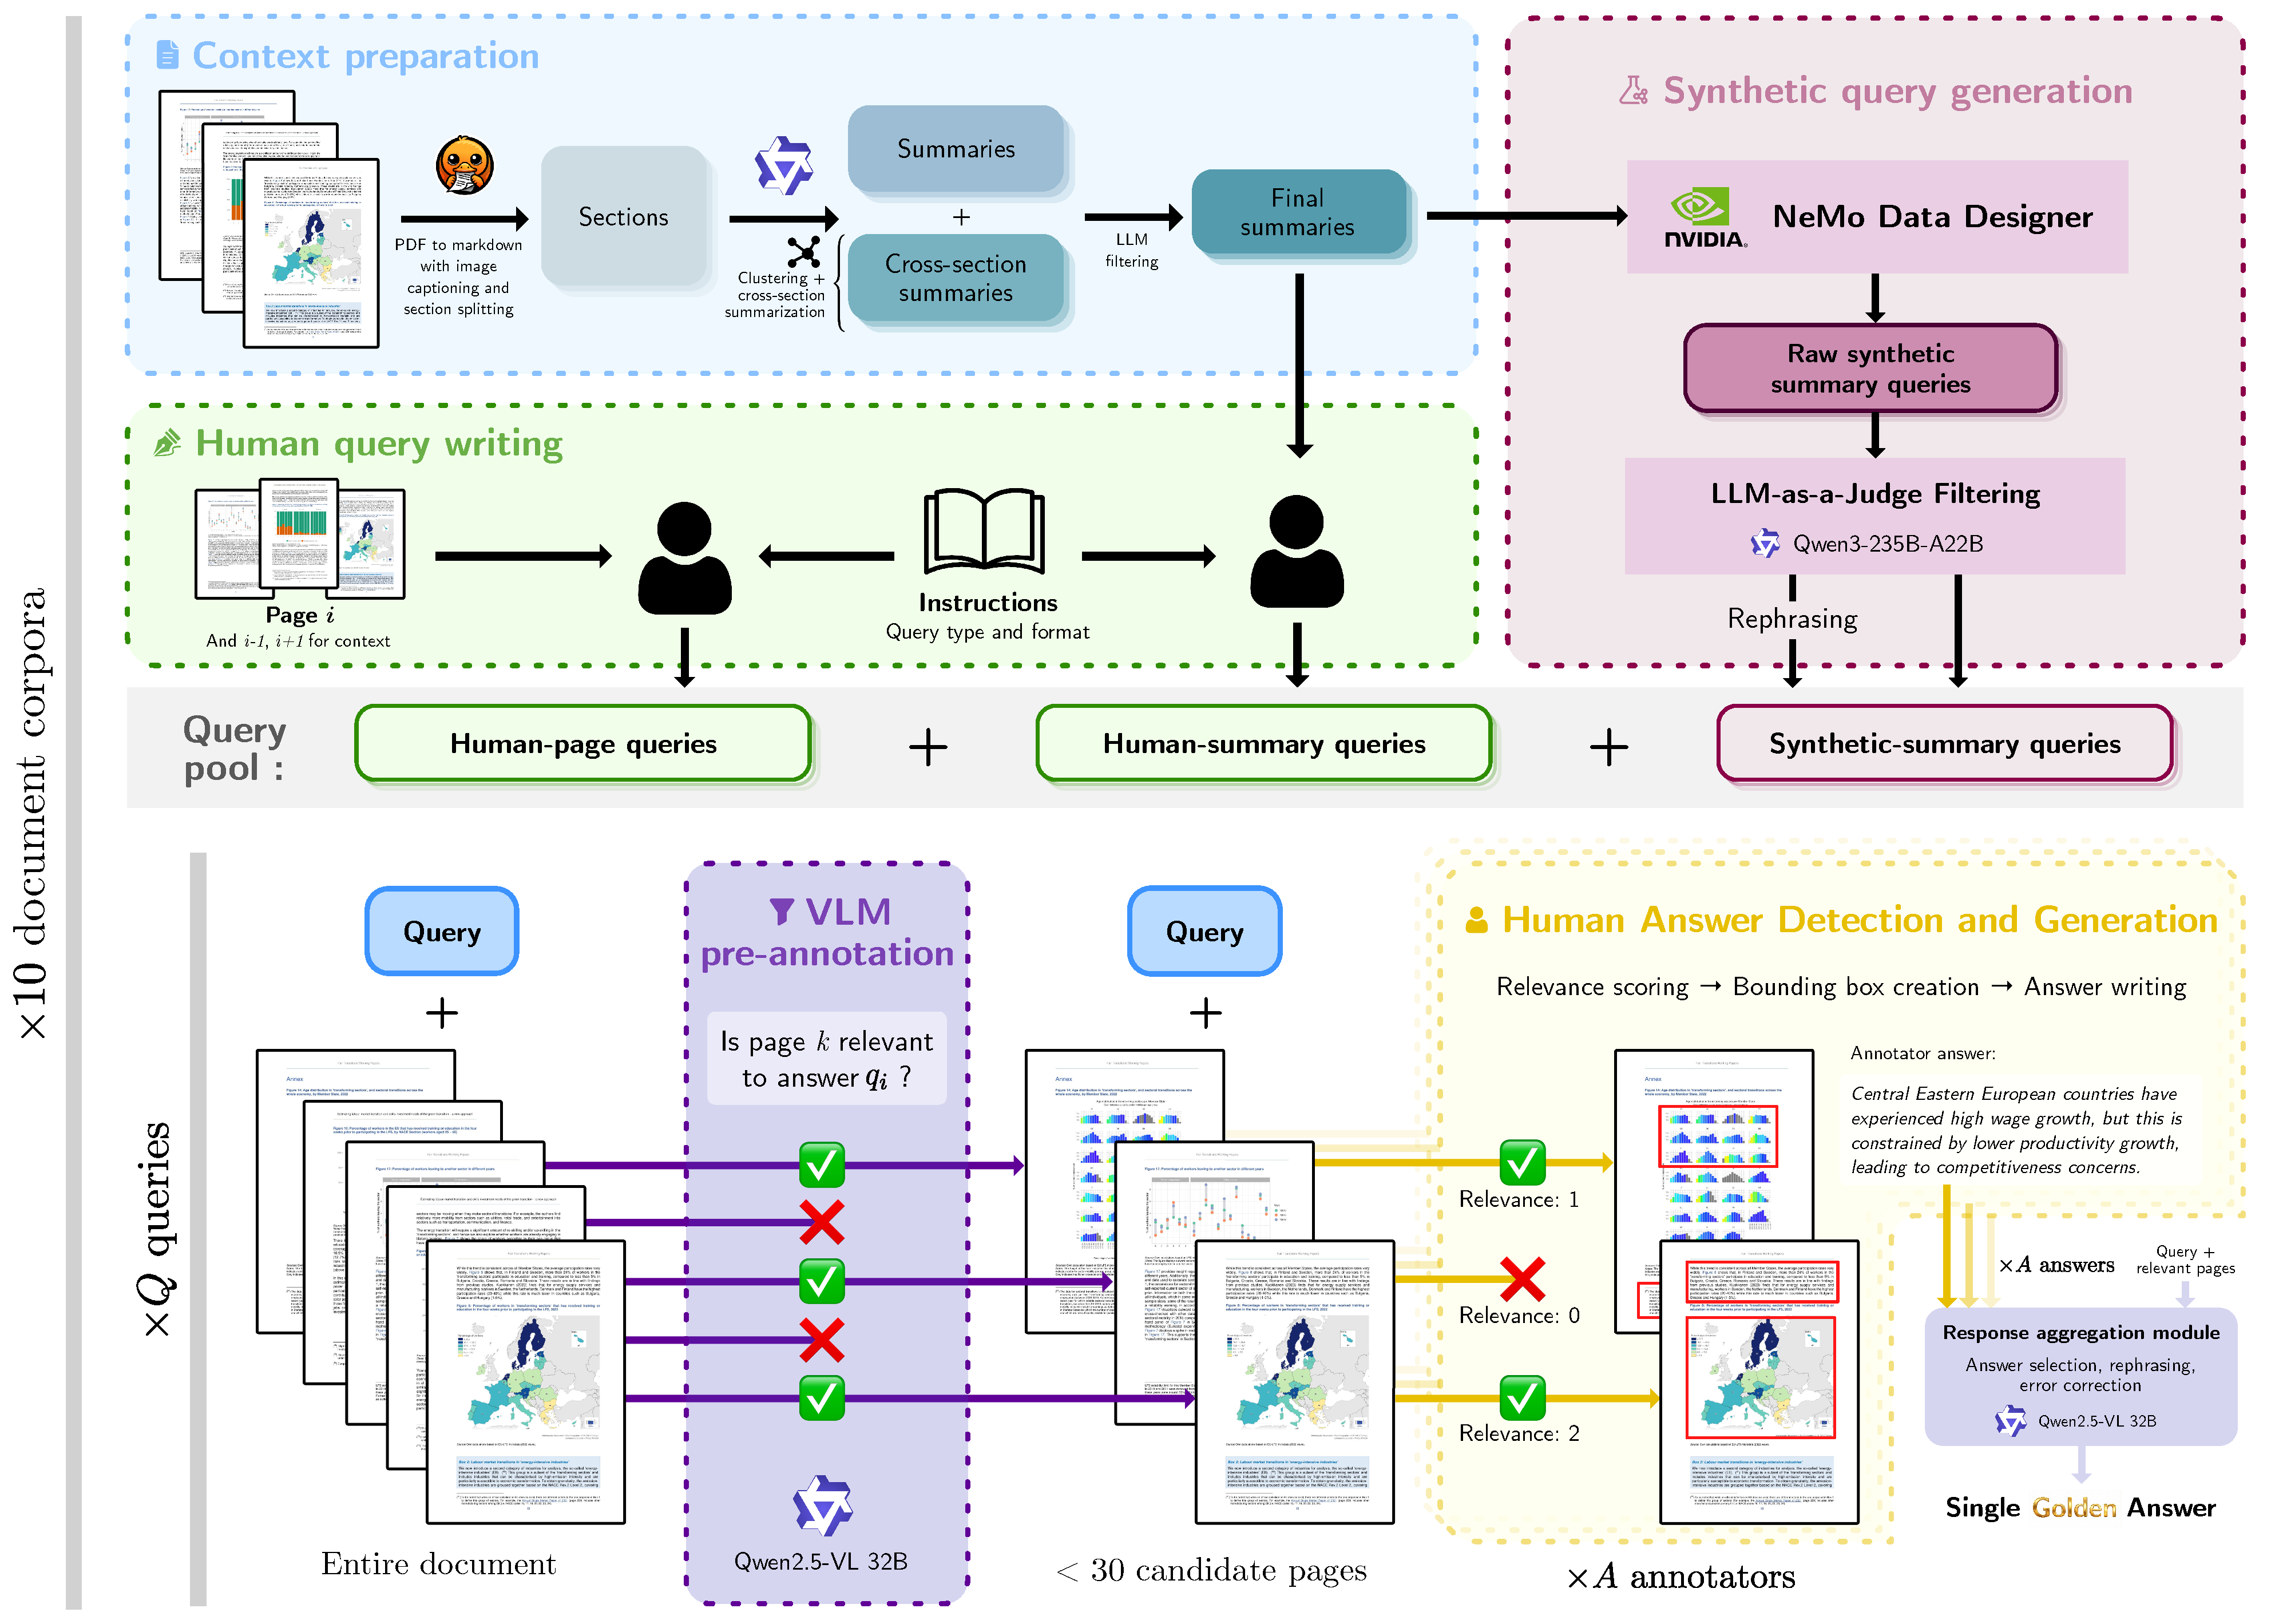
\includegraphics[width=\textwidth]{images/vidorev3_images/dataset-generation-vf.pdf}
    \caption{\textbf{Overview of the benchmark creation process.} Queries are sourced from 3 streams: \textit{human extractive} (using raw pages), \textit{human blind contextual} (using summaries to mitigate extractive bias), and \textit{synthetic blind contextual}. For each query, a VLM pre-filtered subset of candidate pages is labeled by 1--3 human annotators that perform relevance scoring, bounding box localization and answer generation. A final response aggregation combines annotator answers into a single answer.} %\gmor{Could you identify in the main figure what are Tasks 1 and Task 2?}\anto{Yes, it would be great to reuse the terms Query Writing and Query Linking}}
    \label{fig:full process}
\end{figure*}

To address these limitations, we introduce \textbf{\vidorev}, a benchmark designed for complex and realistic end-to-end RAG evaluation on visually rich document corpora. Our contributions are:

% A Scaled Human-in-the-Loop ... (pas ouf, j'aime bien le realistic mais tous les titres deviennent trop longs) on a un peu de place ici
% A Novel Human... methodo for realistic/complex? queries
% From Claude: One small consideration: some reviewers find "novel" unnecessary since contributions are expected to be new. pas faux
\paragraph{1. A Human Annotation Methodology for Realistic Queries} We propose an annotation protocol for generating diverse queries and fine-grained query-page annotations. By restricting annotator access to document content during query formulation, we capture authentic search behaviors and mitigate bias toward simple extractive queries. Vision-Language Model (VLM) filtering combined with human expert verification enables efficient, high-quality annotation at scale.

%\paragraph{1. A Complete Human-in-the-Loop Annotation Methodology.} We introduce a novel human-in-the-loop methodology designed to capture authentic information-seeking behaviors rather than simple fact-verification. By restricting the information available to annotators during query formulation, we mitigate the bias toward trivial, purely extractive questions. This protocol combines Vision-Language Model (VLM) pre-filtering with expert human verification to efficiently produce high-quality retrieval relevance, bounding box grounding, and verified reference answers at a significant scale.
% \paragraph{1. A Complete Human-in-the-Loop Annotation Methodology.} We introduce a novel annotation protocol that combines Vision-Language Model (VLM) pre-filtering with expert human verification. This methodology allows for the creation of high-quality, fine-grained annotations \manu{at large scale? / processing large volumes of data to select from?}. It includes retrieval relevance, bounding box grounding, and verified reference answers at a scale and depth previously unattained for complex document tasks. \anto{maybe a bit too enthusiastic}
\paragraph{2. The ViDoRe V3 Benchmark} Applying this methodology to 10 industry-relevant document corpora, we build ViDoRe V3, a multilingual RAG benchmark comprising ~26,000 pages and 3,099 queries, each available in 6 languages. Two datasets are held out as a private test set to mitigate overfitting. The public datasets are released under a commercially permissive license.  %The benchmark is fully integrated into the MTEB ecosystem and leaderboard \sidecite{muennighoff2023mteb}, and the public datasets are released under a commercially permissive license.
\paragraph{3. Comprehensive Evaluation and Insights} Leveraging our granular annotations, we benchmark state-of-the-art models on \textbf{(i)} retrieval accuracy by modality and language, \textbf{(ii)} answer quality across diverse retrieval pipeline configurations, and \textbf{(iii)} visual grounding fidelity. Our analysis surfaces actionable findings for RAG practitioners.


% \anto{Gautier's comment: Add in intro a sentence / short paragraph of why we focus on "enterprise" (realistic, where IR has the most value, difficult, messy, ...), if this wording is used throughout the text} Retrieval-Augmented Generation (RAG) \sidecite{lewis2021retrievalaugmentedgenerationknowledgeintensivenlp} is now a widely adopted paradigm for knowledge-intensive Natural Language Processing (NLP) tasks  over large document corpora  \sidecite{gao2024retrievalaugmentedgenerationlargelanguage, fan2024surveyragmeetingllms}. However, RAG pipelines deployed in enterprise settings must tackle challenges that extend beyond single document textual retrieval \sidecite{cho2024m3docragmultimodalretrievalneed}. Documents encode critical information in visual elements such as tables, charts, and images designed for human interpretation \sidecite{abootorabi2025askmodalitycomprehensivesurvey}. Additionally, many realistic queries are open-ended, requiring the synthesis, comparison, or explanation of information scattered across multiple documents rather than simple factual answers \sidecite{yang2018hotpotqadatasetdiverseexplainable, wang2023knowledgegraphpromptingmultidocument, tang2024multihopragbenchmarkingretrievalaugmentedgeneration, thakur2025freshstackbuildingrealisticbenchmarks}. \manu{Useful references might include FreshStack (Thakur) that recognize many of the pitfalls in IR benchmarks. The paper might be a nice source of inspiration fot some other refs (and it's quite likely one of the authors is reviewer here).} A further challenge lies in ensuring that generated responses can be reliably traced back to specific source locations within documents, which becomes particularly complex when dealing with visual content rather than plain text \sidecite{gao2023enablinglargelanguagemodels, ma2024visaretrievalaugmentedgeneration}.

% % \begin{figure*}[t!]
% %     \centering
% %     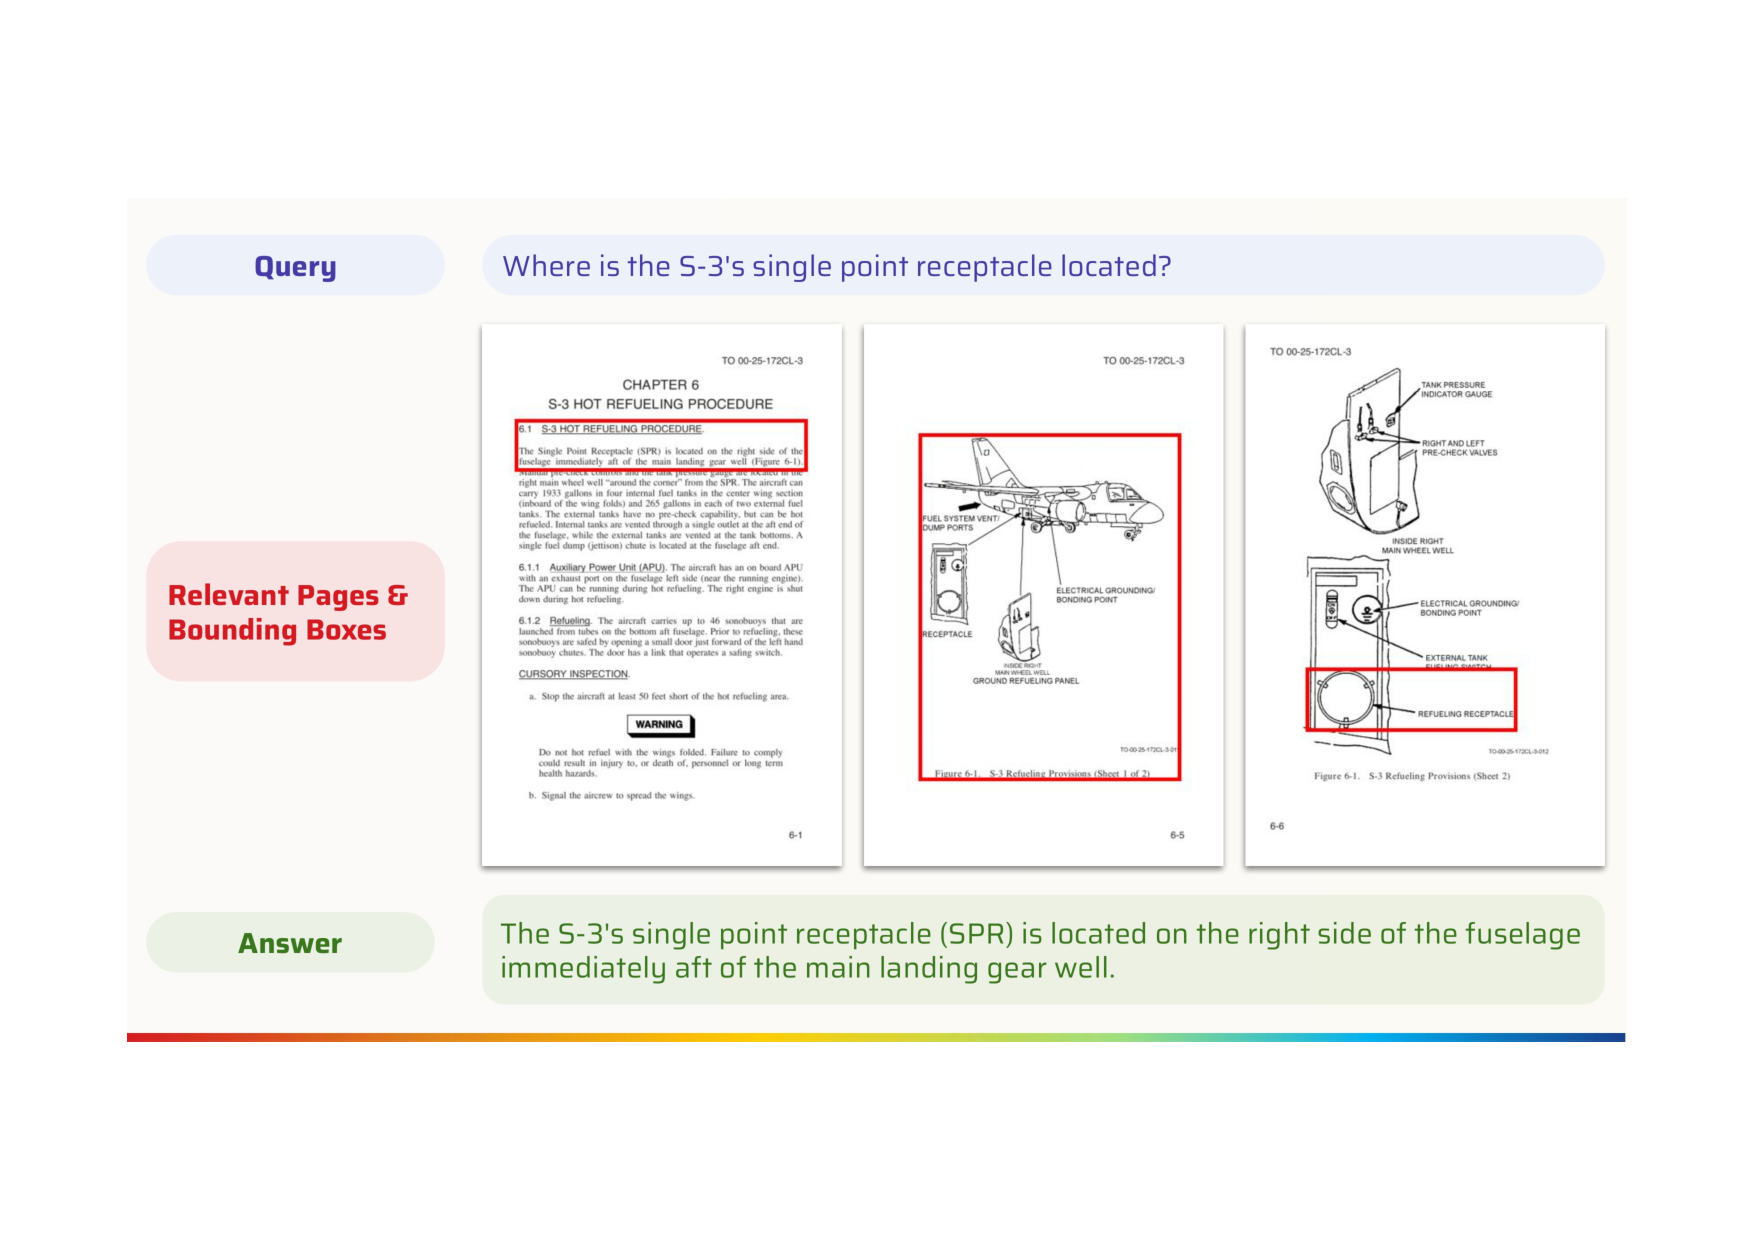
\includegraphics[trim={0cm 2cm 0cm 2cm}, clip, width=\textwidth]{images/vidorev3_images/dataset_overview.pdf}
% %     \caption{\anto{Placeholder for benchmark overview figure, make it single column if possible} \vic{We can use Antoine's figure as the main figure? Just being cautious about the limited space we have}\anto{Examples of samples are mandatory in a benchmark paper like this, I think we can do a single column figure to make it fit cf. \href{here}{https://arxiv.org/pdf/2007.00398}}}
% %     \label{fig:full process}
% % \end{figure*}

% \que{More focus on VISUAL retrieving}\que{need to introduce MM-RAG in the abstract}

% %To address these challenges, we need detailed annotations that cover the 3 main tasks of a MM-RAG pipeline: multimodal retrieval (finding the most relevant contexts for a given query), answer generation (generating an answer to the query based on a set of retrieved contexts) and answer grounding (localizing the parts of the documents that mention the answer to the query). \vic{imo we can remove this paragraph}
% % TODO: rewrite this paragraph well

% However, existing datasets largely fail to capture this end-to-end complexity. Early visual visual document understanding datasets \sidecite{mathew_docvqa_2020, wang2024charxiv} focus primarily on single-page comprehension, ignoring the retrieval challenges of large corpora. Conversely, recent retrieval-centric benchmarks \sidecite{faysse2025colpaliefficientdocumentretrieval, macé2025vidorebenchmarkv2raising, günther2025jinaembeddingsv4universalembeddingsmultimodal} isolate the search component, overlooking the subsequent generation and grounding quality. DUDE \sidecite{van2023document} and M3DocRAG \sidecite{cho2024m3docrag} extend evaluation to multi-page settings but remain largely extractive, emphasizing short factoid answers over the multi-step reasoning and synthesis demanded by open-ended enterprise queries. While contemporary works such as UniDocBench \sidecite{peng2025unidocbenchunifiedbenchmarkdocumentcentric} have made strides toward end-to-end evaluation including summarization tasks, they remain limited to a single language and lack visual grounding annotations necessary to diagnose hallucination in complex layouts. Some benchmarks \sidecite{ma2024visaretrievalaugmentedgeneration, yu2025bboxdocvqalargescale} address the issue of visual grounding but they are far from enterprise domains.
% % While early multimodal benchmarks have attempted to provide ways of evaluating these tasks, they often fail to capture the full complexity of enterprise-level RAG. Document-based question answering benchmarks such as DocVQA \sidecite{mathew_docvqa_2020} and CharXiv \sidecite{wang2024charxiv} focus primarily on single-image understanding. More recent datasets, including M3DocVQA \sidecite{cho2024m3docrag} and DUDE \sidecite{van2023document}, extend to multi-page documents but remain largely extractive, emphasizing short answers that do not stress multi-step reasoning or synthesis. Recent document retrieval benchmarks \sidecite{faysse2025colpaliefficientdocumentretrieval, macé2025vidorebenchmarkv2raising} isolate retrieval performance, largely overlooking answer generation quality, grounding fidelity, and query diversity. Among contemporary works, UniDocBench \sidecite{peng2025unidocbenchunifiedbenchmarkdocumentcentric} offers the most significant end-to-end evaluation across industry domains; however, it remains constrained by a focus on extractive questions and a single language. \anto{Not really just extractive, they also have summarization and comparison}

% To address this gap, we introduce the following contributions:
% % \manu{Bullet points are a waste of paper space, you won't find them a lot in most papers cause it means you had space to spare}
% \paragraph{Contribution 1} We release \textbf{ViDoRe V3}, a comprehensive RAG benchmark emphasizing open-ended queries on long-form, visually rich document corpora. It is composed of 10 datasets from diverse industry domains, totaling about 26,000 document pages paired with 3,099 unique queries available in 6 languages. \manu{do we want to include something about the fact is representative of existing RAG use cases ? ie. domains are diverse but also carefully chosen} It contains fine-grained expert \que{is the expert ok here?} human annotations developed through a 12,000-hour annotation process, including relevant page annotations for retrieval, bounding boxes for visual grounding, and verified reference answers (Section~\ref{sec:benchmark creation}).
% \paragraph{Contribution 2} Using benchmark annotations, we evaluate \textbf{(i)} retrieval accuracy, providing insights into the effects of pipeline modality, query language and type, and context modality and length (Section~\ref{sec:retrieval results}), \textbf{(ii)} final answer generation and how it varies with retrieval pipeline design choices (Section~\ref{sec:visual grounding results}), \textbf{(iii)} visual grounding based on bounding box localization accuracy (Section~\ref{sec:visual grounding results}). \manu{Contrib 1 is meant to enable this so this is not a contribution on its own. what is a contribution is to evaluate "current models / current pipelines to gather actionnable practicle insights". }

% \manu{I believe one of the selling points and the novelty of this paper lies in the "method" behind the annotation and this is what we can insist in as a contribution. Figure 2 perfectly goes with my point here."Novel methodology to produce high quality RAG annotations at scale using human in the loop and AI agents etc etc. Remember that Vidore v2 was never published so all contribs of v2 can be used in this paper directly I believe this "methodology as a novelty" angle is the one that will be of interest to the ACL reviewers. Personnaly, this would be contrib 1 to me, then the benchm,ark as 2, then the insights as 3 --> clear storyline.}

% \anto{Gautier's comment: Vidore V2 is on arxiv so not sure we can reuse them as contributions of this paper}
% \que{Don't think VidoreV2 being on arxiv prevents us from describing this as a contribution, the approach is much more fine grained and tuned than for v2 (with actual human in the loop, and not just an António in the loop)}

% \paragraph{Contribution XXX} \que{Construction work :} We describe a new human-in-the-loop annotation process for realistic end-to-end RAG benchmark combining pre-filtering via VLM into fine grained human annotations. We purposedly limit information available at query generation time to prevent query being really specific or plainly extractive. 


% To foster community adoption, ViDoRe V3 is fully integrated in the MTEB \sidecite{muennighoff2023mteb} ecosystem. Retrieval results are publicly available on a dedicated MTEB leaderboard\footnote{\href{https://mteb-leaderboard.hf.space/?benchmark_name=ViDoRe(V3)}{Leaderboard link} \gmor{I think we should make the URL explicit here, as the paper might be printed}\que{I think the link should be anonymous for submission} \anto{YES}}. 


% \begin{table*}[t]
% \small
% \centering
% \renewcommand{\arraystretch}{0.9}
% \begin{tabular}{p{2cm}cccccc}
% \toprule
% & \makecell{\textbf{MMLongBench} \\ \scriptsize\sidecite{ma2024mmlongbenchdocbenchmarkinglongcontextdocument}}
% & \makecell{\textbf{MIRACL-VISION} \\ \scriptsize\sidecite{osmulski2025miraclvisionlargemultilingualvisual}} & \makecell{\textbf{JinaVDR} \\ \scriptsize\sidecite{günther2025jinaembeddingsv4universalembeddingsmultimodal}} & \makecell{\textbf{Vidore V1} \\ \scriptsize\sidecite{faysse2025colpaliefficientdocumentretrieval}} & \makecell{\textbf{Vidore V2} \\ \scriptsize\sidecite{macé2025vidorebenchmarkv2raising}} & \makecell{\textbf{ViDoRe V3} \\ \scriptsize(this work)} \\
% \midrule
% PDF Documents & \Checkmark &  & \partially & \partially & \Checkmark & \Checkmark \\ \midrule
% % Different Query Types & \questionmark & \questionmark & \questionmark & \questionmark & \questionmark & \questionmark & \Checkmark \\ \midrule
% % Different Query Formats & \questionmark & \questionmark & \questionmark & \questionmark & \questionmark & \questionmark & \Checkmark \\ \midrule
% Multi page Queries & \Checkmark & Sometimes & Sometimes & & \Checkmark & \Checkmark \\ \midrule
% Multi document Queries & & & & & & \Checkmark \\ \midrule
% Answers & \Checkmark & & & & & \Checkmark \\ \midrule
% Grounding Bounding Boxes &  & & & & & \Checkmark \\ \midrule
% Human Verification & \Checkmark & & \partially & & \Checkmark & \Checkmark \\ \midrule
% Commercially Open License & & \Checkmark & & \partially & & \Checkmark \\ \midrule
% Average retrieval space & \questionmark & \questionmark & \questionmark & \questionmark & \questionmark & \questionmark \\ \midrule
% Number of pages per query & \questionmark & \questionmark & \questionmark & \questionmark & \questionmark & \questionmark \\
% \bottomrule
% \end{tabular}
% \caption{Comparison of Visual Retrieval Benchmarks. \anto{Should I add this benchmark \href{https://huggingface.co/datasets/llamaindex/vdr-multilingual-test}{llamaindex benchmark} ?}\anto{How would we add a row for query diversity}\anto{The first row means checks if the corpus is based on real world pdfs}\anto{Maybe we can find a way of presenting }\anto{Improve presentation of criteria column}} % Existing benchmarks don't cover all the criteria for enterprise evaluation
% \label{table:benchmark_comparison}
% \end{table*}

\section{Related Work}

\paragraph{Component-Level Benchmarks (VDU and Retrieval)} VDU has traditionally relied on single-page datasets like DocVQA \sidecite{mathew_docvqa_2020}, alongside domain-specialized variants \sidecite{mathew2021infographicvqa, zhu_towards_2022, wang2024charxiv}. These ignore the multi-page context inherent to RAG. Recent work evaluating bounding-box source grounding \sidecite{yu2025bboxdocvqalargescale} proposes single-page and multi-page tasks but does not address the retrieval component. Conversely, the emergence of late-interaction visual retrievers \sidecite{ma2024unifyingmultimodalretrievaldocument, faysse2025colpaliefficientdocumentretrieval, yu2024visragvisionbasedretrievalaugmentedgeneration, xu2025llamanemoretrievercolembedtopperforming} spurred the creation of retrieval-centric visual benchmarks like Jina-VDR  \sidecite{günther2025jinaembeddingsv4universalembeddingsmultimodal} and \vidore \space V1\&V2  \sidecite{ faysse2025colpaliefficientdocumentretrieval, macé2025vidorebenchmarkv2raising}, but none of these benchmarks jointly evaluate retrieval and answer generation.
% yet no existing visual RAG benchmark jointly evaluates retrieval and answer generation. % faux cf. unidoc bench
%failing to evaluate the downstream generation quality required to synthesize grounded answers.
%While valuable, these ignore the corpus-scale retrieval inherent to RAG; even recent work evaluating bounding-box source grounding \sidecite{yu2025bboxdocvqalargescale} remains confined to single-page contexts.

\paragraph{End-to-End Multimodal RAG} While recent textual RAG benchmarks now capture complex user needs like reasoning or summarizing \sidecite{thakur2025freshstackbuildingrealisticbenchmarks, tang2024multihopragbenchmarkingretrievalaugmentedgeneration, su2024bright}, multimodal evaluation often remains limited to single page queries \sidecite{faysse2025colpaliefficientdocumentretrieval}. Multi-page datasets like DUDE \sidecite{van2023document}, M3DocRAG \sidecite{cho2024m3docragmultimodalretrievalneed}, ViDoSeek \sidecite{wang2025vidorag} or Real-MM-RAG \sidecite{wasserman2025real} prioritize extractive retrieval, lacking the diversity of queries encountered in realistic settings. 
UniDocBench \sidecite{peng2025unidocbenchunifiedbenchmarkdocumentcentric} represents a concurrent effort that similarly addresses diverse query types and provides comparative evaluation across multiple RAG paradigms. While this benchmark offers valuable contributions, it relies on synthetically generated queries via knowledge-graph traversal, is restricted to English documents, and constrains grounding annotations to parsed document elements. In contrast, our benchmark offers several complementary strengths: fully human-verified annotations, multilingual coverage, free-form bounding box annotations, and a more systematic evaluation of individual visual RAG pipeline components.

%UniDocBench \sidecite{peng2025unidocbenchunifiedbenchmarkdocumentcentric} is a concurrent benchmark featuring diverse query types and a comparative evaluation of multiple RAG paradigms. However, the queries are synthetically generated via knowledge-graph traversal, the benchmark is English-only, and grounding is limited to parsed document elements. Our benchmark provides fully human-verified annotations, multilingual coverage, free-form bounding boxes, and we conduct more systematic evaluations of visual RAG pipeline components.


\section{Benchmark Creation} \label{sec:benchmark creation}

We design the benchmark to mirror the diversity of information retrieval situations in large-scale realistic environments. To enable pipeline-agnostic evaluation of the 3 core RAG components (retrieval, generation and grounding), while avoiding limitations of synthetic benchmarks, we employ a rigorous three-stage human-in-the-loop annotation process involving document collection, query generation and grounded query answering (\Cref{fig:full process}).

%The goal is to obtain annotations that can help assess the 3 main components of RAG pipelines: information retrieval, answer generation and answer grounding while being agnostic to the type of pipeline used. To avoid problems of preceding synthetic benchmarks and produce high-quality queries, we design a meticulous human annotation involving 3 steps: document collection, query generation and grounded question answering as described by \Cref{fig:full process}.

% TODO: rewrite this paragraph well

\subsection{Document Collection}

We curate 10 diverse corpora by manually selecting openly-licensed documents from governmental, educational, and industry sources, focusing on English and French documents (7 and 3 corpora respectively). The corpora span Finance, Computer Science, Energy, Pharmaceuticals, Human Resources, Industrial Maintenance, Telecom, and Physics. Each features domain-specific terminology and document structures representative of realistic retrieval tasks (details in \Cref{tab:datasets}).
%\footnote{See Appendix \ref{tab:datasets} for corpus details}.

%To reproduce enterprise scenarios and facilitate enterprise adoption, we created the 10 domain corpora by manually selecting documents from governmental, educational and enterprise websites that met our open license criteria. Each corpus focuses on a well-defined domain with specialized terminology and document structures that are representative of real-world industrial document retrieval tasks\footnote{A detailed breakdown of each corpus is provided in Appendix \ref{tab:datasets}.}. Our focus was on a English-French collection, so 7 corpora were selected in English and 3 in French. Domains cover a wide range of enterprise sectors including Finance, Computer Science, Education, Nuclear Energy, Pharmaceuticals, Human Resources, Industrial Maintenance, Telecom and Physics.
% TODO: rewrite this paragraph well

\subsection{Query Generation}

% \paragraph{Query and Task Diversity}
% \que{TODO : merge with 2.3}
% Unlike traditional retrieval benchmarks that treat user intent as monolithic, the benchmark recognizes that complex enterprise queries often layer multiple formats and types. As detailed in Section \ref{sec:query_generation}, we classified queries using a multi-label taxonomy of 7 distinct types across 3 formats.

\paragraph{Query Taxonomy} To evaluate document visual retrieval systems across diverse realistic scenarios, we develop a query taxonomy with two orthogonal dimensions: \textit{Query Type}, defining the user's information need, and \textit{Query Format}, describing the query's syntactic structure. This dual-axis classification enables more nuanced performance analysis than benchmarks focusing solely on interrogative extractive queries. We define 7 Query Types: \textit{open-ended}, \textit{extractive}, \textit{numerical}, \textit{multi-hop}, \textit{compare-contrast}, \textit{boolean}, and \textit{enumerative}, and 3 Query Formats: \textit{question}, \textit{keyword}, and \textit{instruction}. % that reflect modern search engine usage \vic{last part to justify or remove}\footnote{Taxonomy details are described in \Cref{tab:query_taxonomy}}. % To generate even more diverse queries, a synthetic and human query generation processes were followed.

%\paragraph{Query Taxonomy} A primary objective of our benchmark is to evaluate document visual retrieval systems across a comprehensive spectrum of real-world search scenarios. To achieve this, we first develop a detailed query taxonomy that classifies queries along two orthogonal dimensions: \textit{Query Type}, which defines the user's underlying information need, and \textit{Query Format}, which describes the syntactic structure of the query itself. This dual-axis classification allows for a more nuanced analysis of model performance than benchmarks that focus solely on interrogative extractive queries.



% The objective of this benchmark is to get several types of queries that cover different several search engine usages. We listed 7 query categories : 

% \begin{itemize}
%     \item \textbf{open-ended}: an explanatory or descriptive query that synthesizes  information; may be broad in scope and focused on qualitative aspects of the summary,
%     \item \textbf{extractive}: a clear and specific query that can be answered using only a specific piece of information.
%     \item \textbf{compare-contrast}: a query that requires comparing and/or contrasting multiple entities or topics that are closely related to each other
%     \item \textbf{boolean}: a yes/no query that may involve multiple steps of reasoning.
%     \item \textbf{numerical}: a query that asks for a specific number or calculated number given a summary. The query should require more than simply reading numbers directly from the page.
%     \item \textbf{multi-hop}: a complex query that requires retrieving and integrating information from multiple sources or steps to produce a complete answer.
%     \item \textbf{enumerative}: a query that asks to list all examples that possess a common property, optionally requesting details about the specifics of each example.
% \end{itemize}

% Most of the benchmarks focus on interrogative queries. However, modern serach engine users use different query formats. We listed the following:

% \begin{itemize}
%     \item \textbf{question}: a complete sentence that ends with a question mark, typically used to seek specific information or clarification,
%     \item \textbf{keyword}: a brief, often fragmented phrase or set of terms used to search or filter information, without forming a full grammatical sentence.
%     \item \textbf{instruction}: a directive that describes a task to be performed on the documents, often in the form of a command or request.
% \end{itemize}

\paragraph{Context Preparation} We further ensure query diversity by pulling summaries from a heterogeneous set of contexts during the generation process.
%Another way of ensuring query diversity is to pull from a heterogeneous set of contexts during the generation process.
Two types of input contexts are used: specific document sections that target local information retrieval and cross-section summaries that target multi-document context retrieval. These summaries are produced through a refined process inspired by ViDoRe V2 \sidecite{macé2025vidorebenchmarkv2raising}. First, the text is extracted from PDFs using Docling \sidecite{auer2024docling} along with image descriptions. Then, summaries are generated with Qwen3-235B-Instruct \sidecite{qwen3technicalreport} from each document section. They are clustered to group similar summaries together using Qwen3-Embedding-0.6B \sidecite{qwen3embedding} as embedder, UMAP \sidecite{mcinnes2020umapuniformmanifoldapproximation} for dimension reduction and HDBSCAN \sidecite{campello2013density} for clustering. Additionally, cross-section summaries are produced by synthesizing the summaries of 2 to 3 randomly selected sections per cluster. From this pool of summaries, a final subset is curated to maintain a strict balance between single-section and cross-section summaries. The selection also ensures an even distribution across section modalities (text, images, and tables) as defined by the Docling element classification.

\paragraph{Synthetic Query Generation} Queries are generated from the summaries using a first synthetic generation pipeline based on Qwen3-235B. For each summary, a prompt is constructed by sampling a query type and format at random, together with variable attributes such as length and difficulty, in order to promote diversity. The generated queries are subsequently evaluated by the same LLM acting as an automatic judge, which filters outputs according to 4 criteria: information richness, domain relevance, clarity and adherence to query type/format. Finally, 50\% of the retained queries are rephrased to further enhance linguistic variance. This pipeline is implemented using NeMo Data Designer \sidecite{nemo-data-designer} to facilitate generation scaling.

\paragraph{Human Query Writing} Human annotators are provided 2 kinds of contexts: synthetic summaries or specific PDF pages. They are tasked with generating one query following a specific query type and format and one query of their choice that is most adapted to the context provided.

% To generate these diverse query types, several specialized data generation pipelines are developed. For extractive queries, human annotators are provided with specific PDF pages, alongside the preceding and succeeding pages for context, and tasked with generating queries in a predefined format and type. For open-ended queries, we follow a refined process introduced in \sidecite{macé2025vidorebenchmarkv2raising}. 

%2 or 3 sections per cluster are randomly selected and the corresponding summaries are summarized to get cross section summaries. From this pool of summaries, a subset of summaries is selected ensuring that single section and cross section summaries are balanced as well as summaries based on a balanced set of modalities: text, images and tables given by the element classification of Docling. For each summary, we prompt Qwen3-235B-A22B-Instruct-2507 \sidecite{qwen3technicalreport} to generate a query given a predefined type and format. We use an LLM-as-a-Judge to filter the synthetic queries and make sure the distribution follows our needs. We also ask humans to generate queries on  these summaries to get diverse queries from different generation processes. \manu{do humans ever verify the query types and format ? could be nice to mention}

%\manu{This is a big blob of text, maybe simolifying a tad and adding details in the appendix, or structruring this a bit more if ytou decide to make this process as a contribiution (human in the loop blablabla)}

\subsection{Answer Detection and Generation} \label{sec: grounded qa}

Queries are filtered and linked to relevant pages using a hybrid pipeline of VLM pre-filtering and human annotation. It is followed by human answer annotation and visual grounding.

% Once queries are generated, they are meticulously linked to relevant pages and bad quality queries are filtered out. The answer to selected queries is also written by human annotators and bounding boxes are drawn around supporting elements in the documents.

% The objective of this annotation phase is to get the relevant pages containing the answer to the query, the bounding boxes that locate the answer in the pages and the answer to the query. \manu{Link this sentence better with the rest of the process. "Once queries are fenerated, we annotate relecant pages as well as the precise bbox and anszwer that are relevant." I would reference figure 2 a bit more throughout and maybe piggyback on it a bit to simplify exolanations.}


%\manu{simolify pgrhasing: human annotation is intractable. We run a first phase of model-assisted and heuristic filters, relying on qwen XXX to remove pages the model deemed irrelevant given a query, and queries that are too broad. We then transmit the remaining queries and associated pages to expert human annotators to obtain a final XXX}.

\paragraph{Query-Page Linking} Given the scale of our corpora, manual verification of each page relevance for each query is intractable. We therefore adopt a two-stage annotation pipeline. First, Qwen2.5-VL-32B-Instruct \sidecite{qwen25vl} pre-filters candidate pages by assessing whether each page image is relevant to the query. Queries whose answers span more than 30 flagged pages are discarded. Human annotators then review the remaining query-page pairs, evaluating query quality and rating page relevance on a three-point scale (Not Relevant, Critically Relevant, Fully Relevant).

%To facilitate human annotation, we first use the Qwen2.5-VL-32B-Instruct VLM \sidecite{qwen25vl}, which is provided with the query and each page image and tasked with determining whether the page is relevant for answering the query. We then discard queries whose answers are spread across more than 30 pages flagged as relevant. The remaining queries and their candidate pages are reviewed by human annotators to produce the final set of relevant pages. Annotators assess query quality and rate page relevance on a three-point scale (Not Relevant, Critically Relevant, Fully Relevant).

%Extractive queries are annotated by at least one annotator and one reviewer, while more complex non-extractive queries are annotated by at least two annotators and one reviewer. A page is retained as relevant if it is marked as such by either (i) one annotator and one reviewer or (ii) at least two annotators.
% simplifying formulation: we run a first phase of model-assisted and heuristic filters, relying on Qwen2.5-VL-32B-Instruct \sidecite{qwen25vl}.

\paragraph{Relevant Page Selection} To ensure annotation quality, each task is completed by multiple annotators and reviewed by annotation supervisors. Since VLM pre-filtering biases the distribution toward relevant pages, we report Gwet's AC2, as it remains stable under prevalence skew, at 0.760 (see \Cref{appendix: relevance agreement} for dataset-level breakdowns). Given this strong but imperfect agreement, we implement a tiered review process: extractive queries require at least one annotator and one reviewer, while more complex non-extractive queries require at least two annotators and one reviewer. A page is retained as relevant if marked by either (i) one annotator and one reviewer, or (ii) at least two annotators.  %\manu{to me this is a detail that should go in app. here we can say double annotation is used to guarantee quality.}\anto{probably to remove}

%Because pages were pre-filtered by a VLM before human annotation, most pages shown to annotators were likely relevant, creating a skewed class distribution. To address this, we report Gwet's AC2 which remains stable under prevalence skew at $0.760$, on average. Details of agreement metrics by domain are given in appendix \ref{appendix: relevance agreement} Given this score, we ensure a safe relevancy annotation by annotating extractive queries by at least one annotator and one reviewer, while more complex non-extractive queries are annotated by at least two annotators and one reviewer. A page is retained as relevant if it is marked as such by either (i) one annotator and one reviewer or (ii) at least two annotators. \manu{to me this is a detail that should go in app. here we can say double annotation is used to guarantee quality.}\anto{probably to remove}



\paragraph{Answer Generation} For each selected query, annotators were tasked with writing an answer based on the pages they marked as relevant. Given that different annotators might have different answer interpretations and tend not to be exhaustive in their answers, we use Qwen2.5-VL-32B-Instruct to generate a final answer based on the relevant page images marked by the annotators and their answers.

%\paragraph{Inter-Annotator Agreement.} Because pages were pre-filtered by a VLM before human annotation, most pages shown to annotators were likely relevant, creating a skewed class distribution. To address this, we report Gwet's AC2 which remains stable under prevalence skew. On average over all domains, annotators achieved an AC2 of $0.760$. \que{Do we still give the other numbers?}\vic{No but need to add a comment interpreting this metric value}Details of agreement metrics by domain are given in appendix \ref{appendix: relevance agreement}

% To filter most of the irrelevant pages, we use a VLM Qwen2.5-VL-32B-Instruct \sidecite{qwen25vl} that is given the query and each page image in the corpus and asked if the page is relevant to answer the query. After this step, we filter out queries whose answers are dispersed on too many pages, more than 30 flagged pages.
% The remaining queries and the corresponding pages are given to a human annotator that filters the final relevant pages. Queries that are tagged as extractive have at least one annotator and one reviewer and others have at least two annotators and one reviewer, as some annotators might miss relevant pages. Only pages that are tagged as relevant by one annotator and one verifier or at least two annotators are kept as relevant. 

\paragraph{Bounding Boxes and Modality Types}
For each relevant page, annotators delineate bounding boxes around content supporting the query and attribute a modality type to each bounding box: Text, Table, Chart, Infographic, Image, Mixed or Other. 
%This process involves a subjective interpretation of which surrounding context should be included.
Because multiple valid interpretations of bounding boxes can exist, we perform a consistency study to evaluate inter-annotator agreement and establish a human performance upper bound for the task.

We compute inter-annotator agreement on the subset of query-page pairs labeled by two or three annotators. For each annotator, we merge all their bounding boxes into a single zone. We then compare zones across annotators by measuring pixel-level overlap, reporting Intersection over Union (IoU) and F1 score (Dice coefficient). When three annotators label the same sample, we average over all pairwise comparisons.

%\anto{precision, recall, F1 are not the right terminology here. According to Gemini, prefer Inclusion Ratio (A in B), Inclusion Ratio (B in A) and Symmetric Agreement Score or Dice Coefficient} \vic{Gemini tells me it's fine with the changes I made. It's more convenient to have an asymmetric metric for the VLM bounding box evaluation.}

%Across all 10 datasets, we observe a mean IoU of 0.50 and F1 of 0.60, with per-dataset IoU (Table~\ref{tab:inter-annotator bbox agreement}) ranging from 0.44 (Physics) to 0.62 (Pharma) \manu{per dateset stats aere details that could be removed if need be}.

Across all 10 datasets, we observe an average IoU of 0.50 and F1 of 0.60. These moderate agreement scores reflect the inherent subjectivity of the task: annotators typically agreed on the relevant content but differed in granularity (Appendix \ref{appendix: bbox examples}), with some marking tight bounds around specific content while others included surrounding context.

\paragraph{Quality Control} The annotation was conducted by a curated pool of 76 domain-qualified experts with native-level language proficiency. Quality control was performed by 13 senior annotators with enhanced domain knowledge and extensive annotation experience. Detailed protocols regarding the annotator pool and training are provided in Appendix \ref{appendix: annotator pool}.

\subsection{Final Query Distribution} 
% \anto{Move some part to the appendix if not enough space}

We conducted a final human review to remove low-quality queries and resolve labeling ambiguities. \Cref{fig:query_type_distribution} shows the resulting distribution. Extractive queries predominate due to human annotator preference, followed by open-ended queries from targeted sampling. Multi-hop queries were the hardest to scale, suggesting a need for dedicated pipelines. \Cref{fig:content_type_distribution} details page modalities; while text is most prevalent, visual elements like tables, charts, and infographics are well-represented.

% A final review stage was conducted to remove remaining low-quality queries and resolve labeling ambiguities, as some queries could belong to multiple types. The final query type distribution is shown in \Cref{fig:query_type_distribution}. Extractive queries are the most represented, as annotators generally preferred this type. Open-ended queries also appear frequently due to targeted sampling to ensure adequate coverage. Multi-hop queries proved most difficult to generate at scale; producing more high-quality examples of this type would require a dedicated pipeline. \Cref{fig:content_type_distribution} shows the modality distribution of relevant pages in the benchmark. Text is the most prevalent modality, but visual elements are well represented, with substantial coverage of tables, charts, and infographics.

%At the end of the process, a final query review is done by reviewers to remove remaining bad queries and relabel query types as some queries can belong to several query types. Final query distribution is shown in \Cref{fig:query_type_distribution}. Query distribution covers all query types but is dominated by extractive ones which were generally preffered by annotators and open-ended queries on which query type sampling emphasized to make sure this type is covered. Multi-hop queries were the hardest to generate because a dedicated pipeline would have to be built to get more good-quality multi-hop queries. \Cref{fig:content_type_distribution} shows the modality distribution of the relevant pages of the benchmark. The most present modality is text, but visual elements are also well covered with a big proportion of tables, charts and infographics.

\begin{figure}[ht]
    \centering
    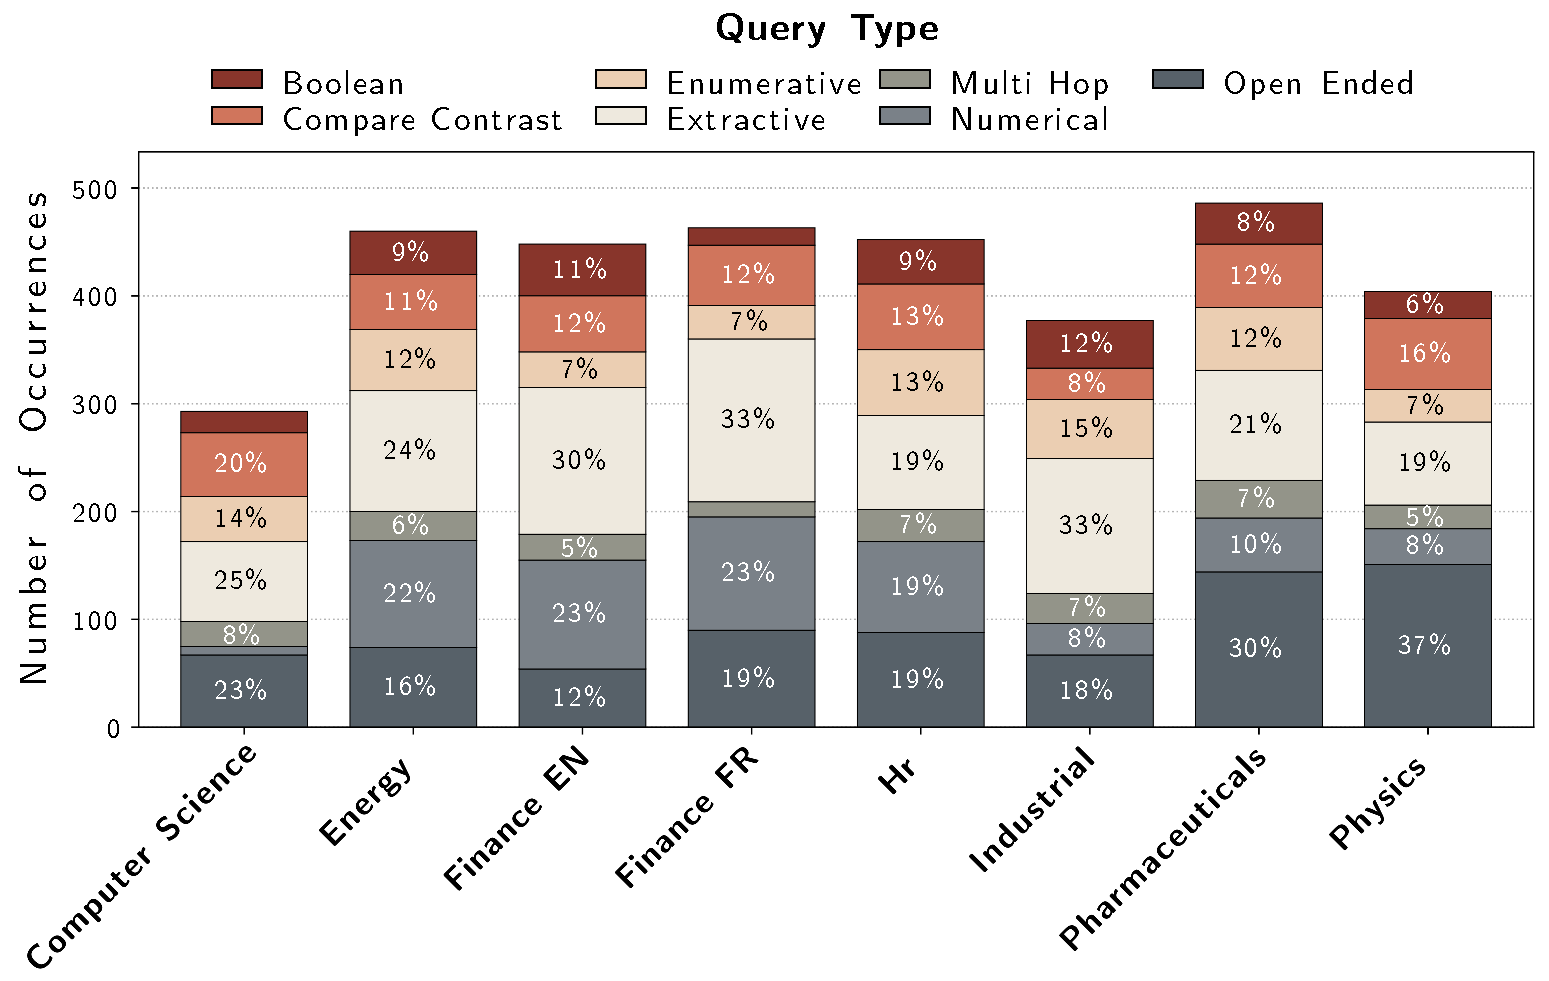
\includegraphics[width=\columnwidth]{images/vidorev3_images/vidore_distribution_acl_v2.pdf}
    \caption{\textbf{Query Type Distribution per Domain}} 
    \label{fig:query_type_distribution}
\end{figure}

\begin{figure}[ht]
    \centering
    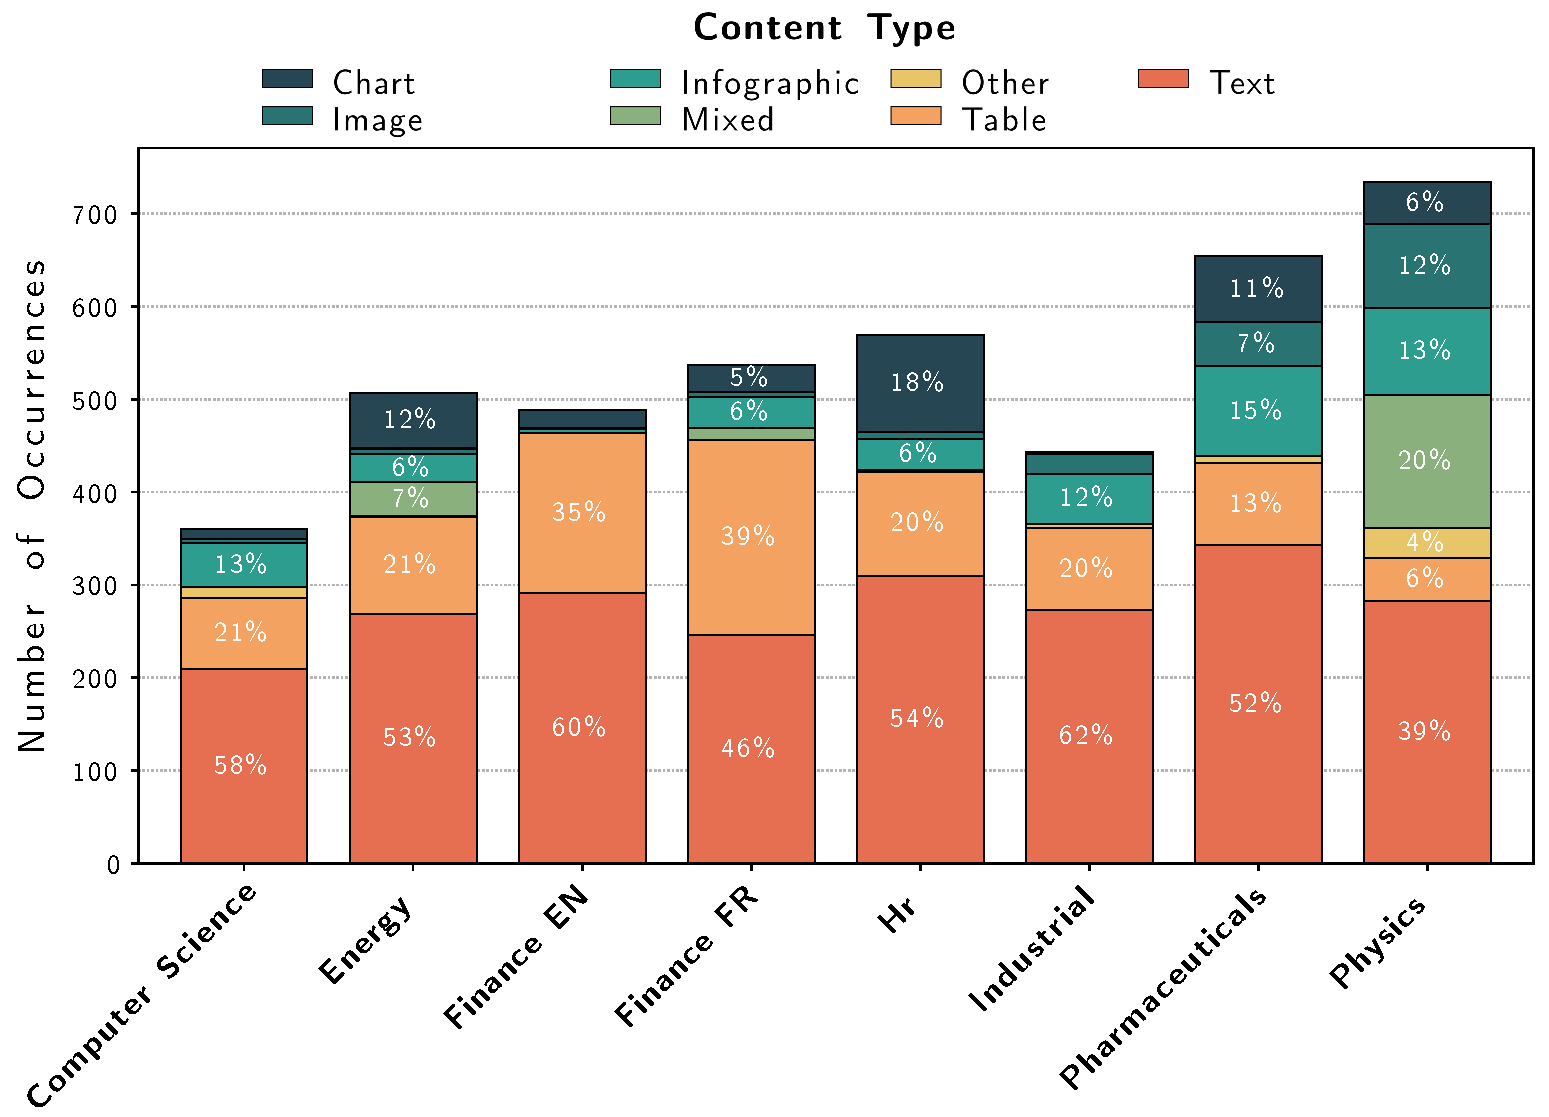
\includegraphics[width=\columnwidth]{images/vidorev3_images/content_type_distribution_acl_v2.pdf}
    \caption{\textbf{Content Type Distribution per Domain}} 
    \label{fig:content_type_distribution}
\end{figure}

% \subsection{Human Annotation}

% \manu{the structure is weird. you mention all the rest and already mention annotators but then have this subsection now. I would perhaps do this the other way around. First put forward human annotators as a jey oart of the pipeline (first thing so it primes readers into trusting the quality), and then detail the various phases. As I mentionned before, I beliebve the entire human in the loop process is a novelty and enables us to produce high qualitry large scale annotations which is not possible without both vompoinents, AI and humns. This could be touched on first, and then detailed. }

%The benchmark was constructed through a two-stage human annotation process designed to produce high-quality queries and reliable ground truth. 

%\paragraph{Annotation Tasks.} The annotation pipeline consisted of two core tasks \gmor{Could you identify in the main figure what are Tasks 1 and Task 2 and reference the image here?}. In the first task, \textit{Query Writing}, annotators reviewed document content and authored queries according to a predefined taxonomy comprising 7 query types and 3 query formats, as detailed in Table~\ref{tab:query_taxonomy}. In the second task, \textit{Query-Page Linking}, annotators performed a comprehensive evaluation: they assessed query quality, rated page relevance on a three-point scale (Not Relevant, Critically Relevant, Fully Relevant), annotated content modalities (Text, Table, Chart, Infographic, Image, or Other), drew bounding boxes around relevant regions, and composed answers to each query. \anto{repeated with 2.3 but better written}


% \paragraph{Annotator Pool and Selection.} Annotation was conducted by a curated pool of 76 annotators who were selected based on having: (1) a bachelor's degree or higher in the relevant domain, (2) professional experience in the domain, (3) native-level language proficiency as required by task, and (4) prior experience with RAG, retrieval, or VQA annotation projects. Quality control was performed by 13 senior annotators with enhanced domain knowledge and extensive annotation experience, with project oversight provided by data leads with multiple years of experience in human data generation. \anto{summarize to one sentence and move the details to appendix}

% \paragraph{Training and Pilot Phase.} The annotation process began with a comprehensive onboarding phase where annotators received task-specific training using gold-standard examples. For each domain, a pilot of several hundred tasks was conducted with 100\% quality control coverage and multiple annotators per task. During this phase, data leads and the research team continuously evaluated annotations, provided clarifications, and refined guidelines. Inter-annotator agreement and time-per-task baselines were calculated to establish ongoing evaluation benchmarks. The pilot concluded upon validation of both data quality and guideline effectiveness. \anto{Move this to appendix}



% \paragraph{Inter-Annotator Agreement.} \anto{We can shorten this and just say that we use Gwet’s AC2 because it's stable under prevalence skew and Weighted Agreement} Because pages were pre-filtered by a VLM before human annotation, most pages shown to annotators were likely relevant, creating a skewed class distribution. This prevalence imbalance causes traditional chance-corrected metrics like Krippendorff's Alpha to appear paradoxically low even when annotators genuinely agree, as inflated expected chance agreement penalizes the score. To address this, we report 3 complementary metrics: Krippendorff's Alpha (ordinal) as the standard measure, Gwet's AC2 which remains stable under prevalence skew, and Weighted Agreement as a raw consistency measure. Overall, annotators achieved $\alpha = 0.469$, AC2 $= 0.760$, and Weighted Agreement $= 0.815$. The divergence between Alpha and AC2/Weighted Agreement is expected given the pre-filtered data and confirms substantial agreement despite the skewed distribution.

\subsection{Dataset Release and Distribution}

%Reflecting the reality of globalized enterprises where knowledge bases are often monolingual while the workforce is distributed\vic{remove this},
We extend the benchmark to rigorously assess cross-lingual retrieval. While source documents are maintained in English and French, we use Qwen3-235B-Instruct to provide translations in 6 languages: English, French, Spanish, German, Italian, and Portuguese. This configuration challenges models to bridge the semantic gap between the query language and the document language, a critical requirement for modern RAG systems. 

Finally, to ensure the integrity of evaluation and mitigate data contamination (which was shown to be a major preoccupation for Information Retrieval \sidecite{rteb2025}), we adopt a split-release strategy. 8 datasets are made public to facilitate research, while 2 are retained as private hold-out sets. This enables blind evaluation, ensuring that performance metrics reflect true generalization rather than overfitting to public samples.

%Finally, to ensure the integrity of evaluation and mitigate data contamination (which was shown to be a major preoccupation for Information Retrieval \sidecite{rteb2025}), we adopt a split-release strategy. 8 datasets are made public to facilitate research, while 2 are retained as private hold-out sets. This enables blind evaluation via the MTEB leaderboard, ensuring that performance metrics reflect true generalization rather than overfitting to public samples.

% \subsection{Cross-Lingual Extension} \vic{TODO Quentin combine with following subsection}.

% Real-world enterprise knowledge bases are often dominated by English or dominant local languages, while the workforce can be globally distributed. To assess cross-lingual retrieval capabilities, the benchmark includes source documents in both English and French, paired with queries in 6 different languages ({English, French, Spanish, German, Italian, and Portuguese}). This setup challenges models to bridge the semantic gap between the query language and the document language, a critical requirement for globalized RAG systems.

% \subsection{Benchmark Splitting}

% To ensure the integrity of evaluation and prevent data contamination (which was shown to have a significant impact on IR evaluation \que{CITE MTEB v2}), we adopt a split-release strategy. 8 datasets are publicly released to facilitate research and model development, while two datasets are retained as private hold-out sets. \anto{Which ones?} This design allows for a robust, blind evaluation on the MTEB leaderboard, ensuring that high performance reflects genuine generalization capabilities rather than overfitting to public data distributions.

% \begin{figure*}[H]
%     \centering
%     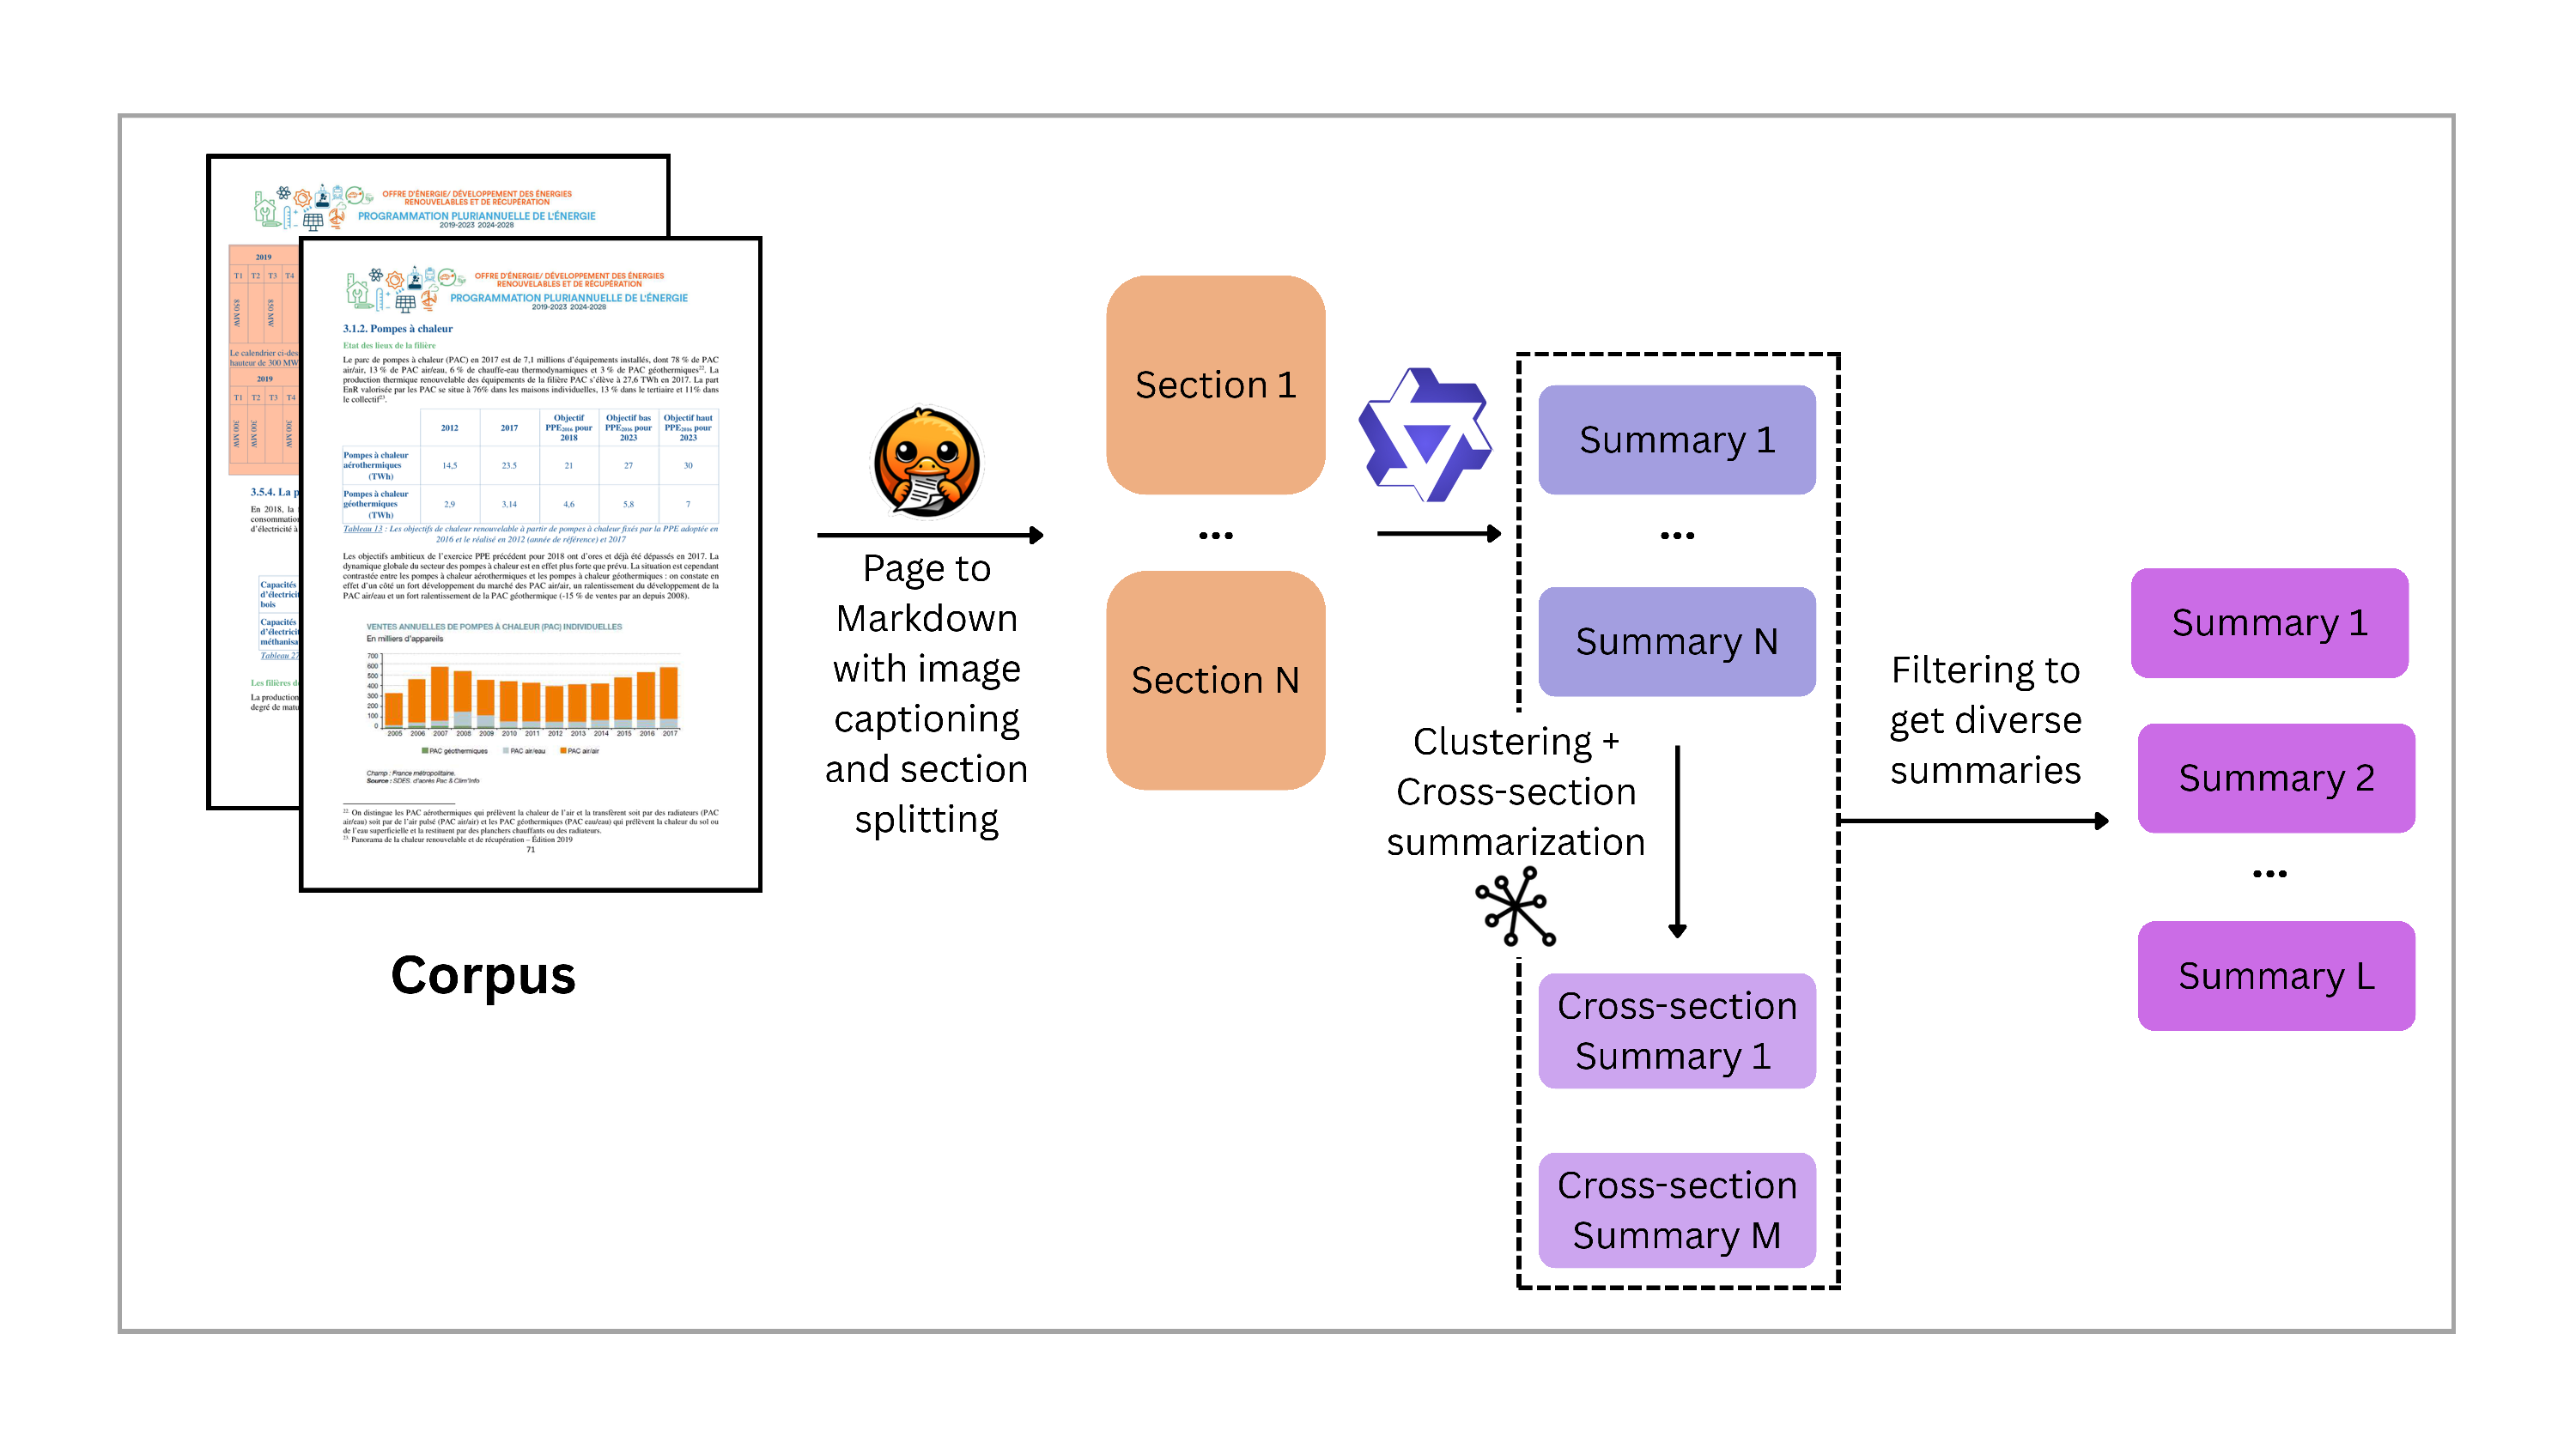
\includegraphics[trim={0cm 2cm 0cm 2cm}, clip, width=\textwidth]{images/vidorev3_images/summary_generation.pdf}
%     \caption{Summarization Process}
%     \label{fig:lf_architecture}
% \end{figure*}

% \begin{figure*}[H]
%     \centering
%     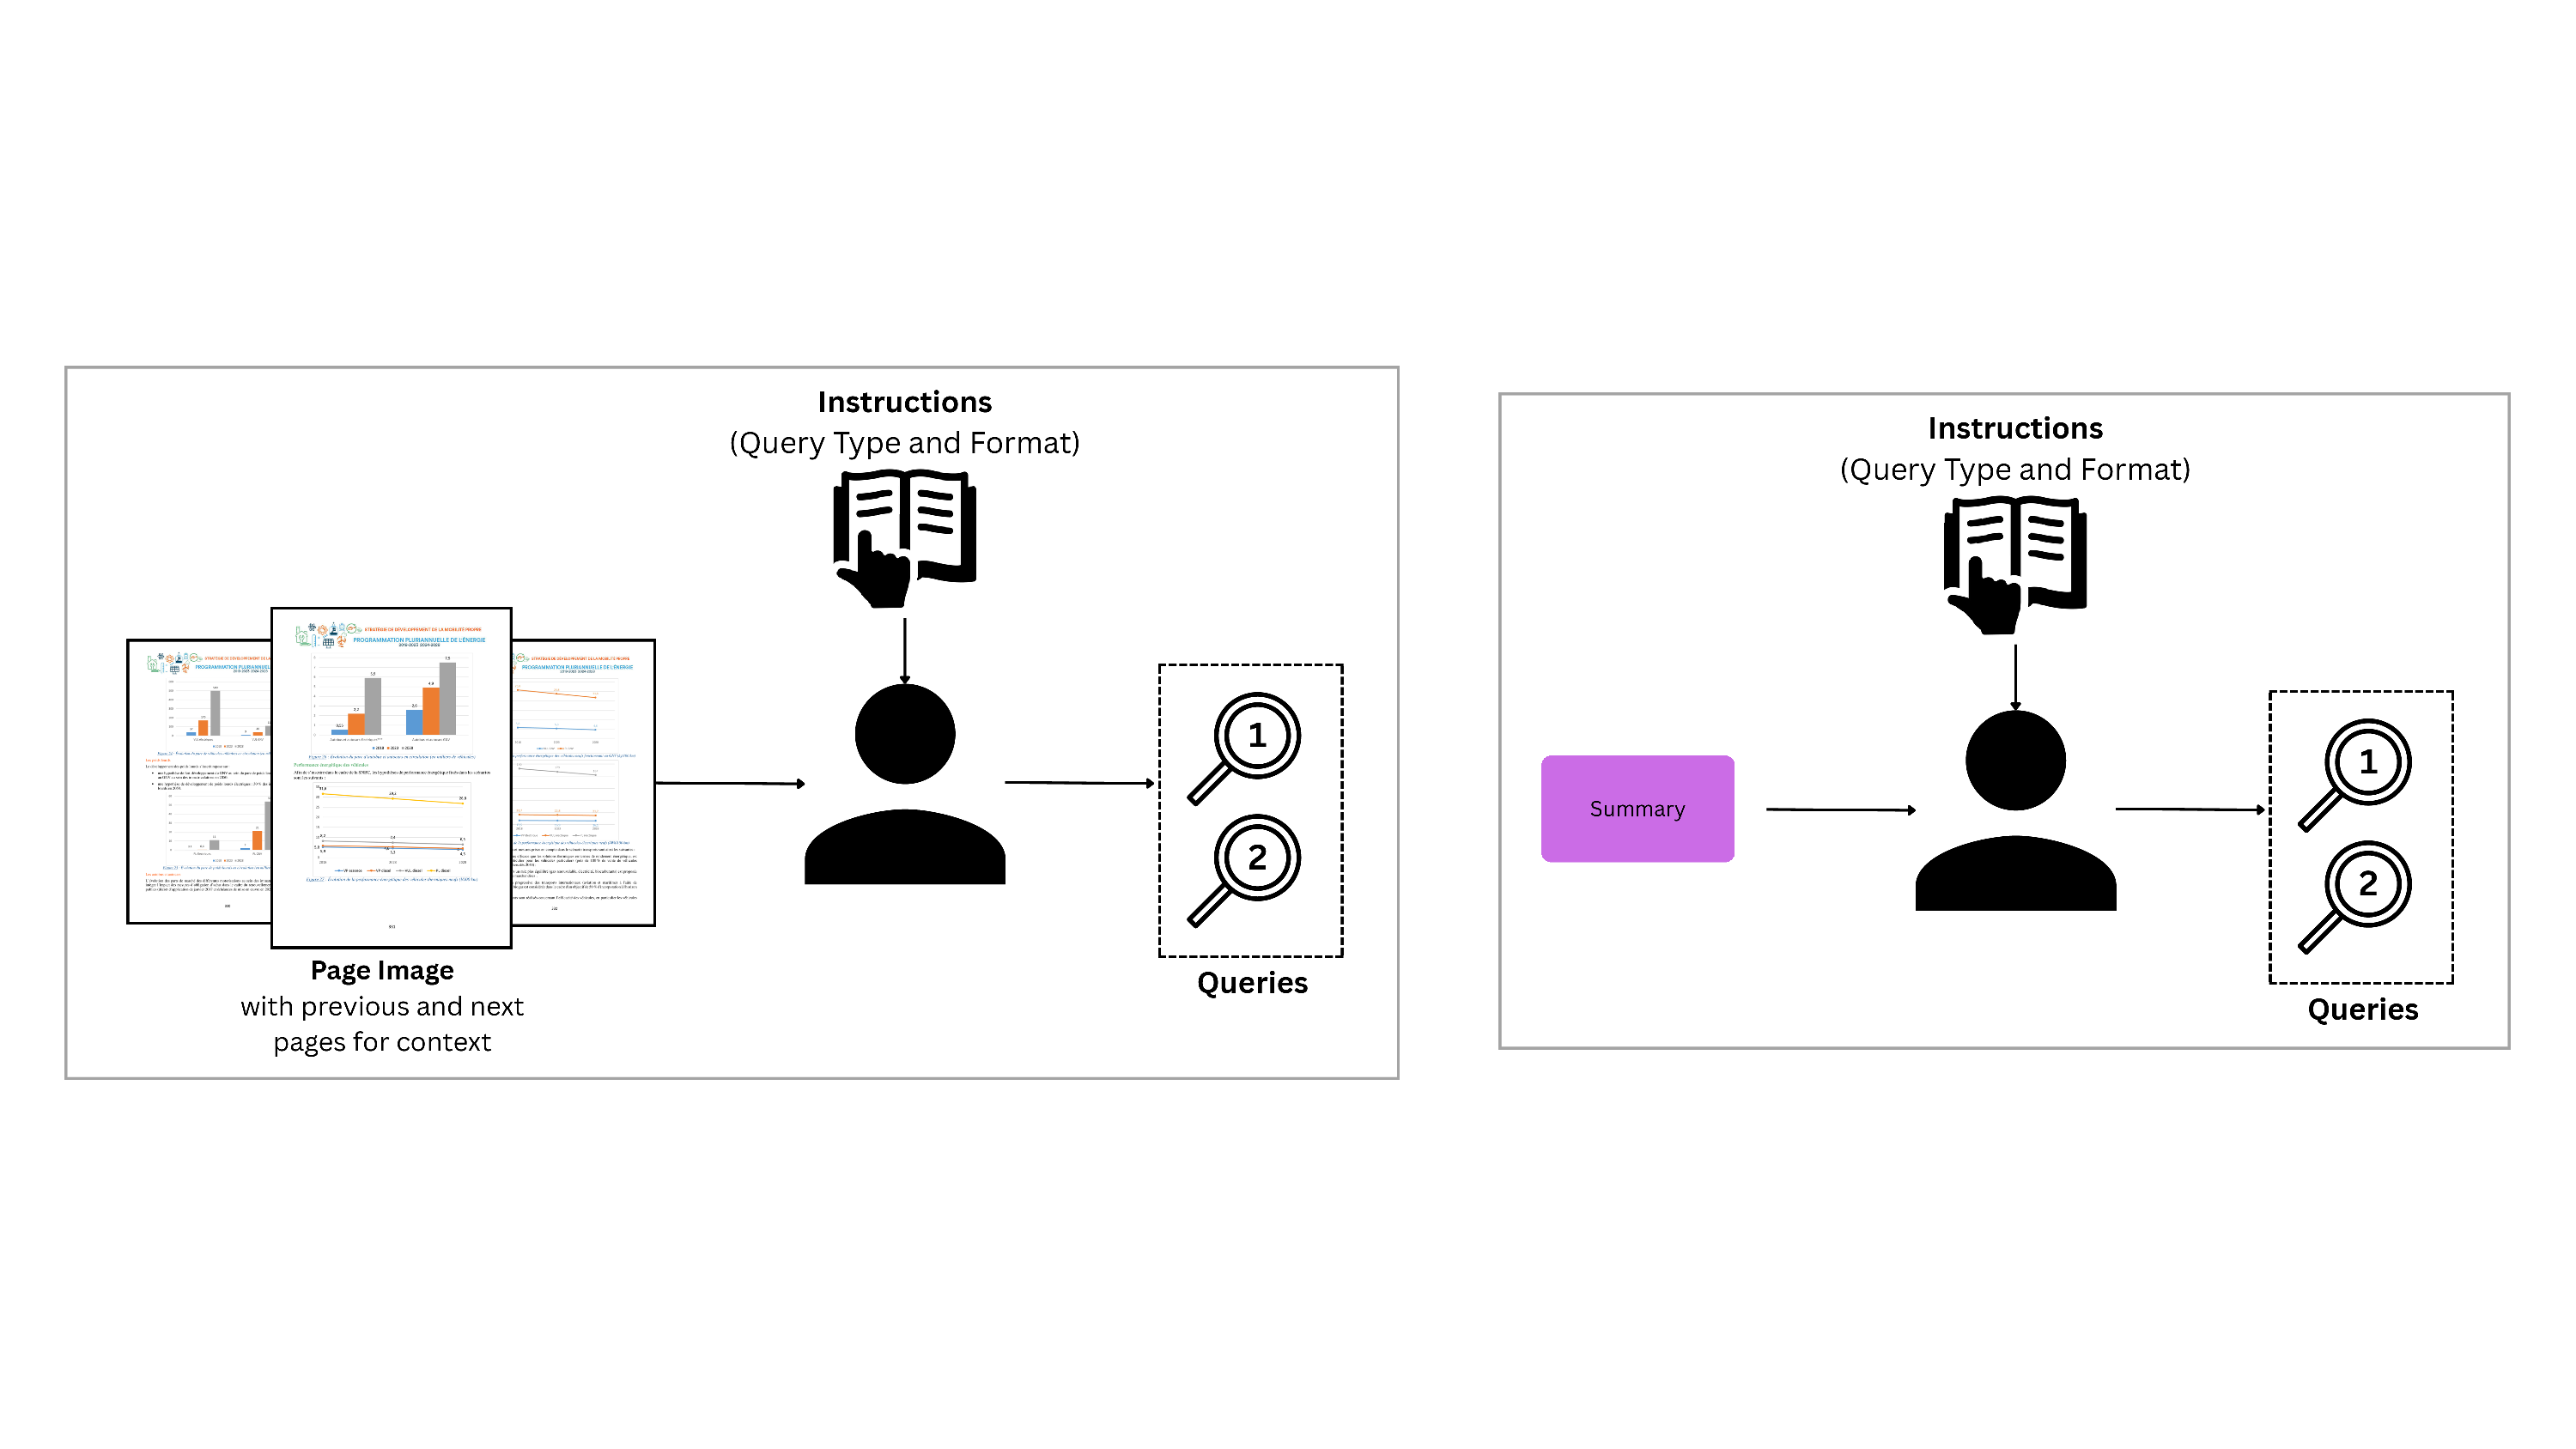
\includegraphics[trim={0cm 7cm 0cm 6cm}, clip, width=\textwidth]{images/vidorev3_images/human_query_generation.pdf}
%     \caption{Human Query Generation Process}
%     \label{fig:query_page_linking}
% \end{figure*}

% \begin{figure*}[H]
%     \centering
%     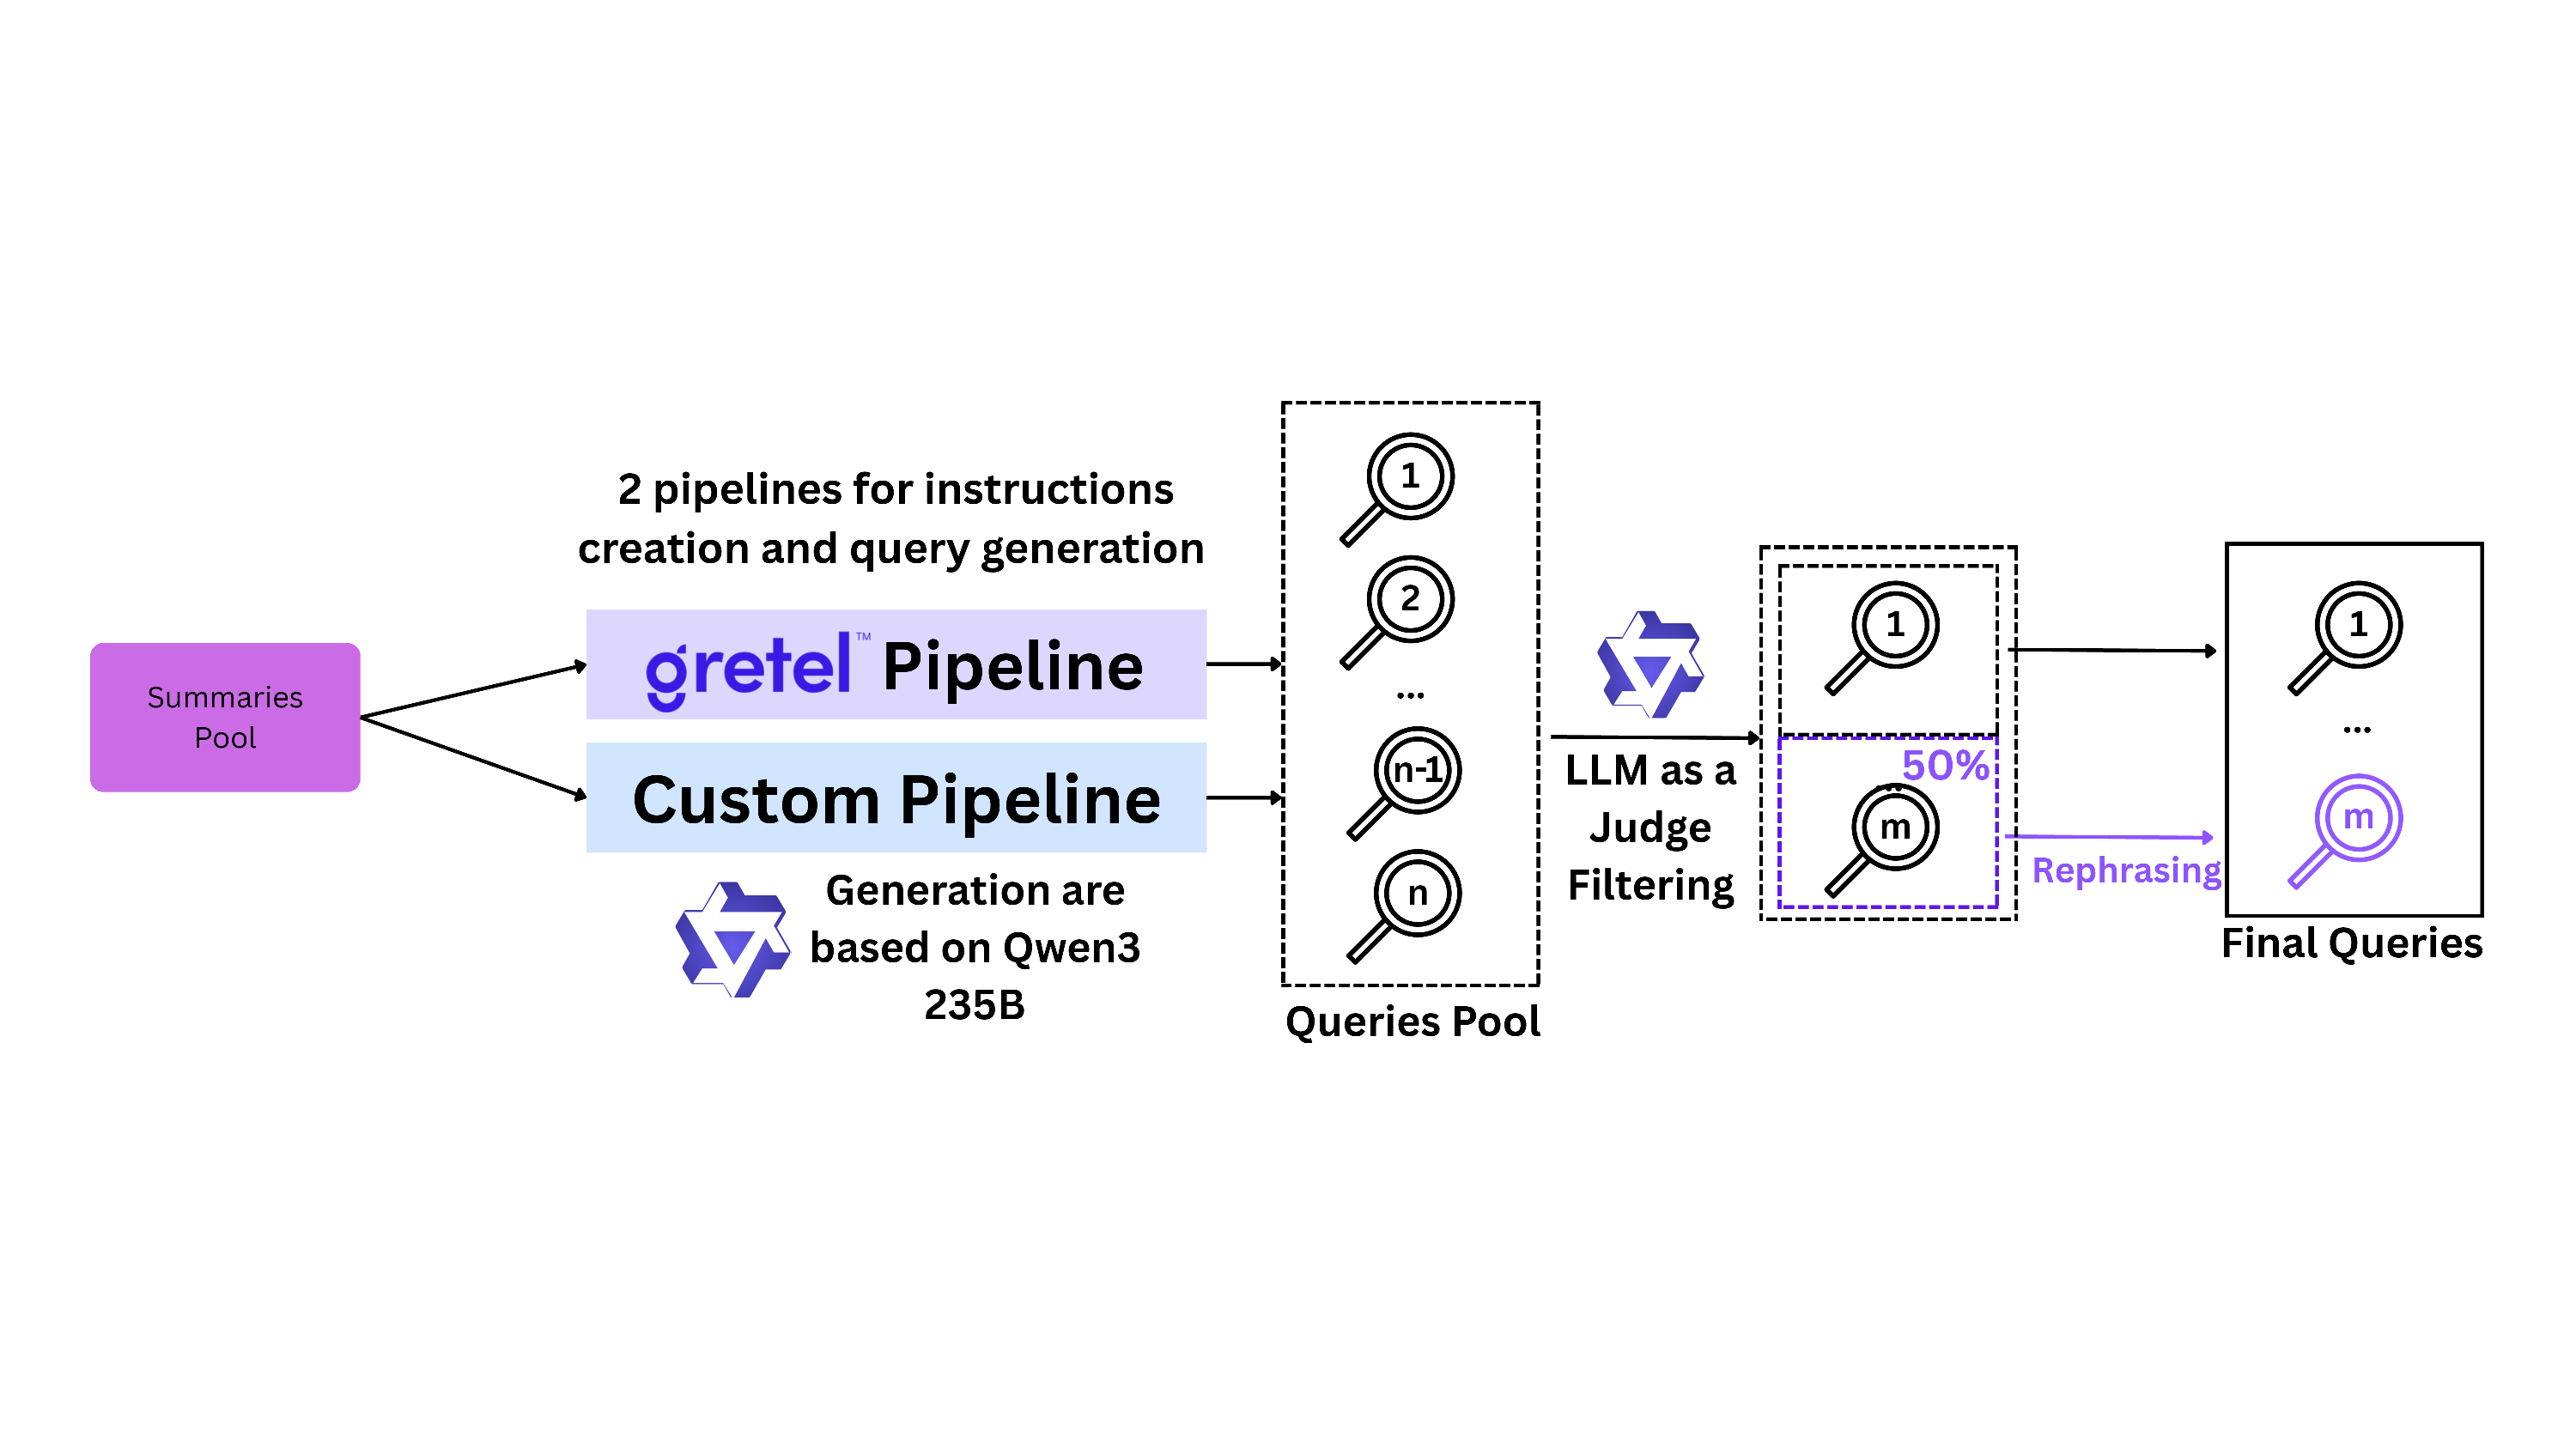
\includegraphics[trim={0cm 7cm 0cm 7cm}, clip, width=\textwidth]{images/vidorev3_images/synthetic_query_generation.pdf}
%     \caption{Synthetic Query Generation Process}
%     \label{fig:query_page_linking}
% \end{figure*}

% \begin{figure*}[H]
%     \centering
%     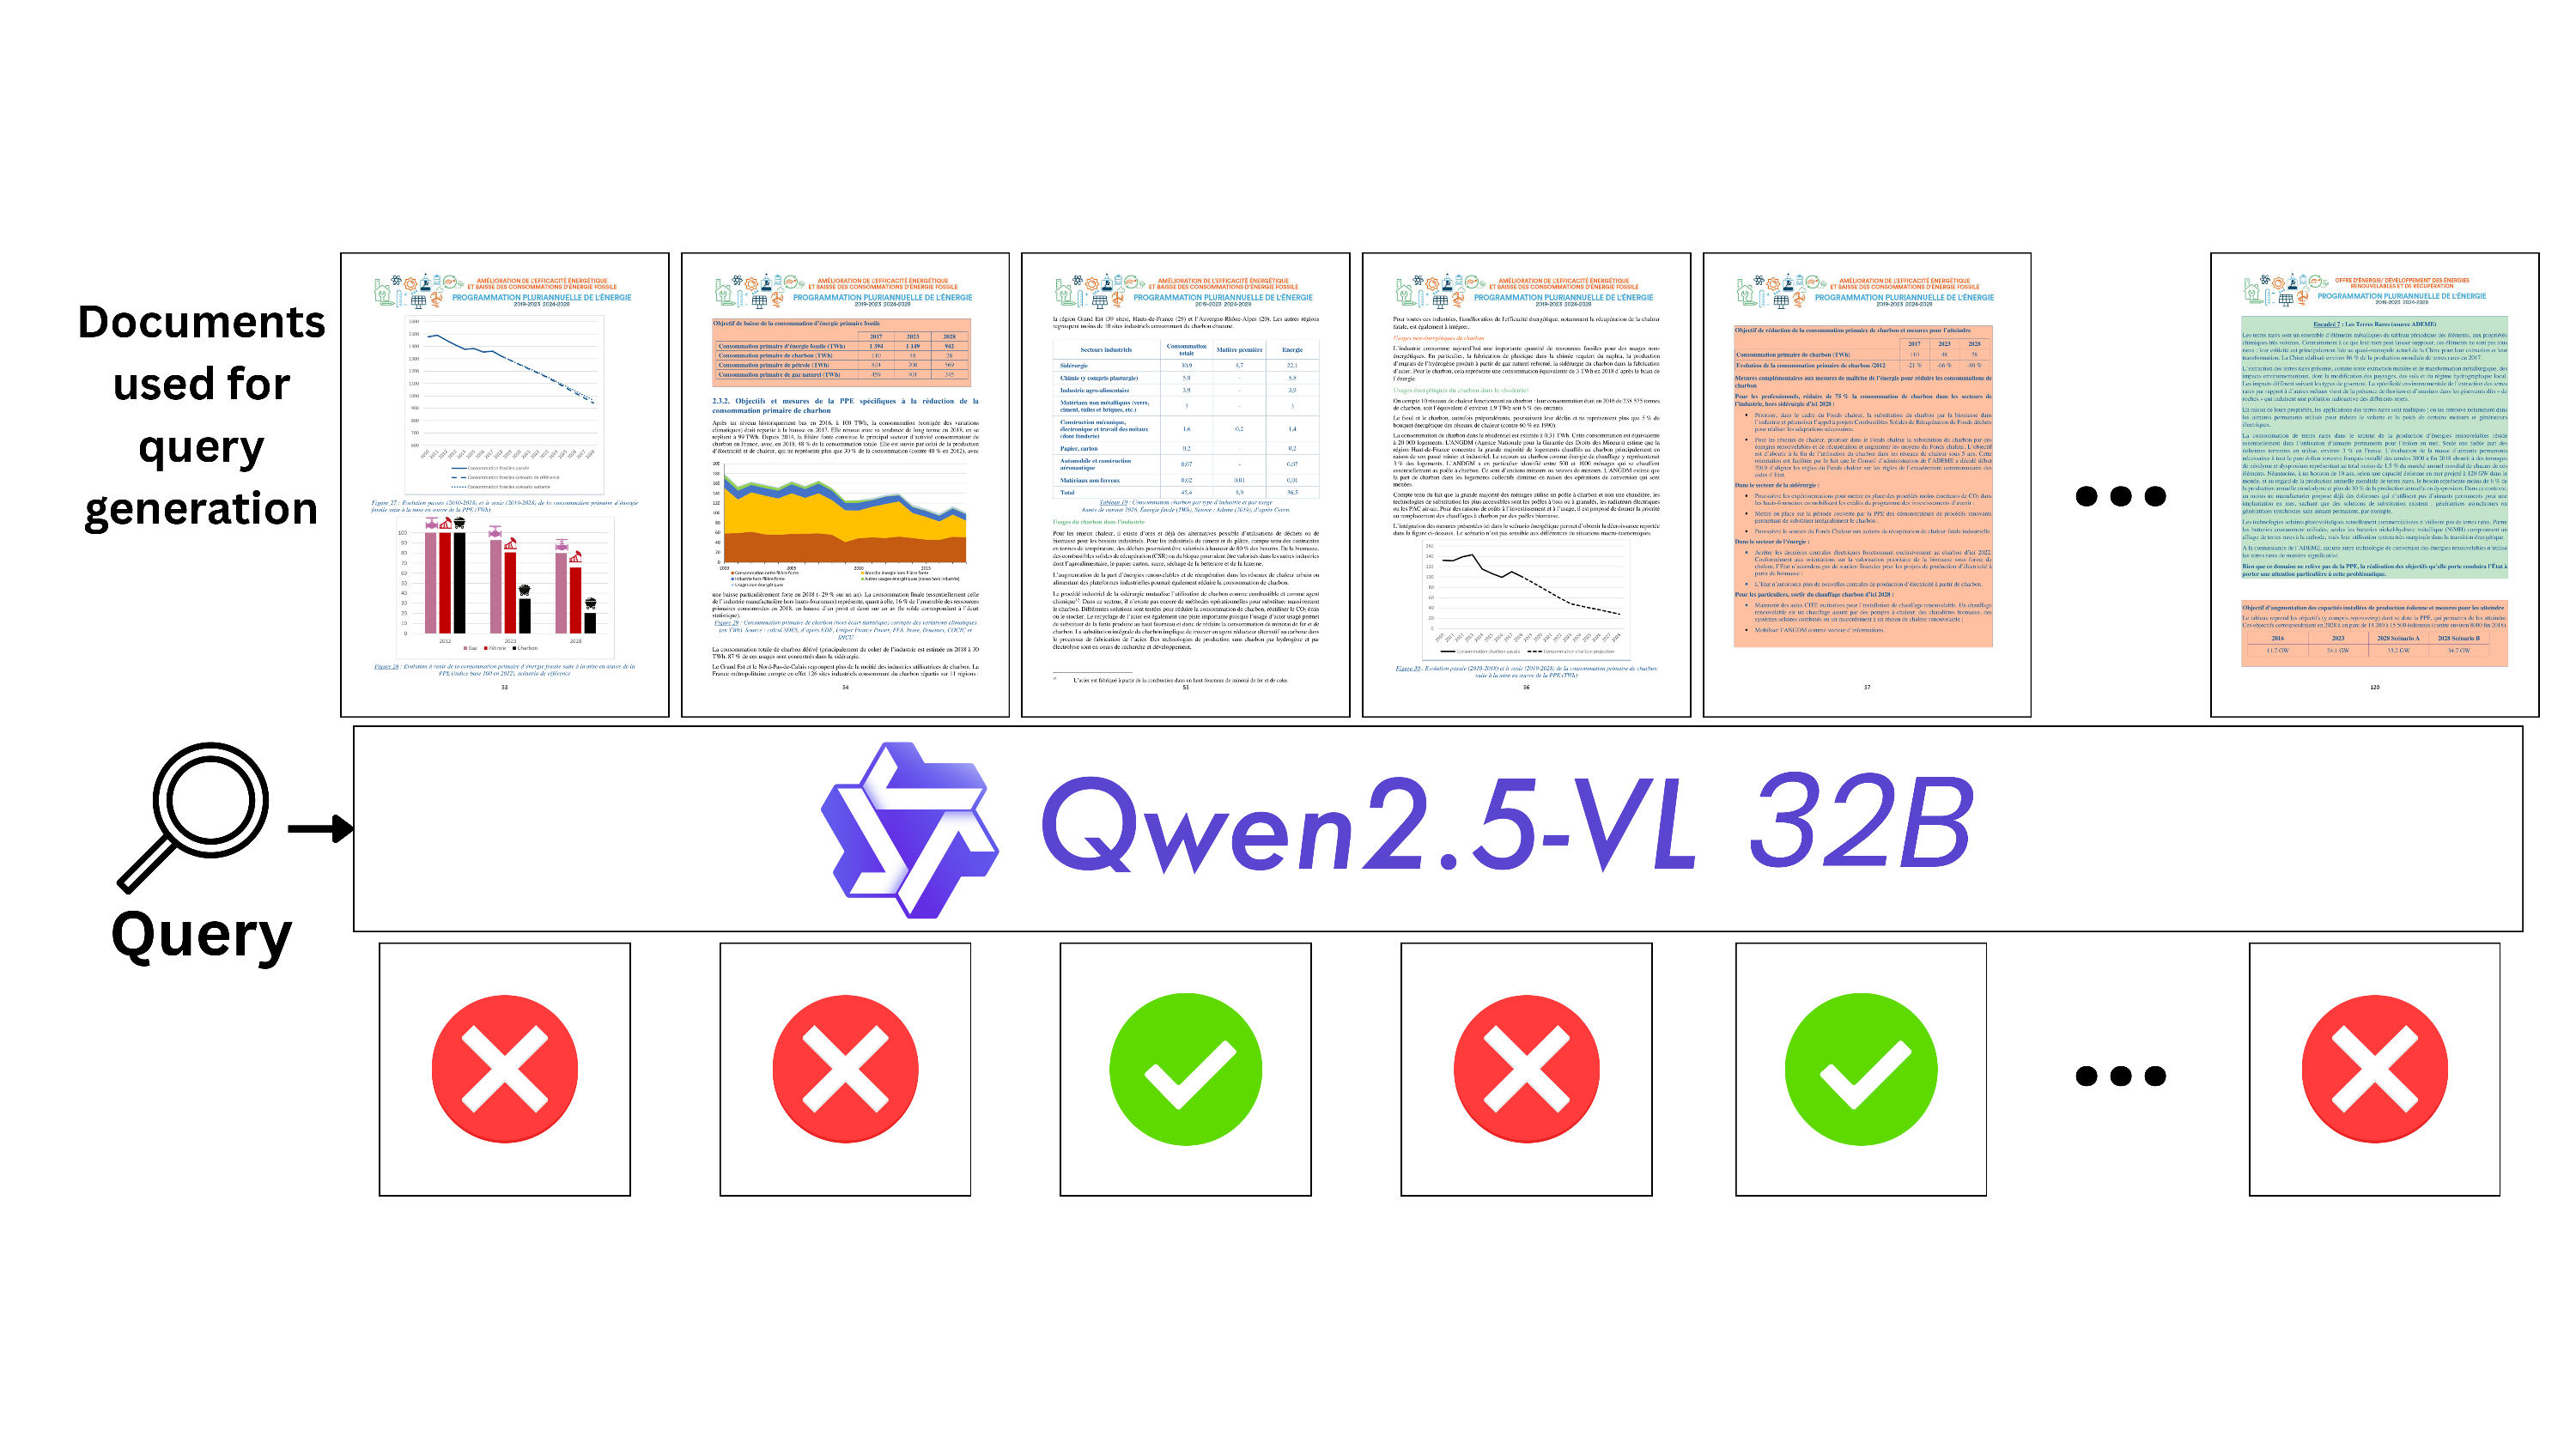
\includegraphics[trim={0cm 4cm 0cm 3cm}, clip, width=\textwidth]{images/vidorev3_images/query_page_linking.pdf}
%     \caption{Query Page Linking Process}
%     \label{fig:query_page_linking}
% \end{figure*}

\section{Experiments and Results}

Using our benchmark, we conduct extensive evaluations across all 3 components of RAG pipelines. We assess textual and visual retrievers and rerankers on retrieval performance, evaluate leading VLMs and LLMs on their ability to generate accurate answers from various retrieved contexts, and test VLMs on bounding box generation for visual grounding. From these results, we compile practical insights for RAG practitioners.

% \begin{figure}[H]
%     \centering
%     \includegraphics{images/vidorev3_images/human_vs_sdg.pdf}
%     \caption{Performance of ColQwen2.5 on human VS SDG queries generated from summaries}
%     \label{fig:lf_architecture}
% \end{figure}

% \begin{figure}[H]
%     \centering
%     \includegraphics{images/vidorev3_images/human_sum_vs_human_img.pdf}
%     \caption{Performance of ColQwen2.5 on human queries from summaries VS human queries from images}
%     \label{fig:lf_architecture}
% \end{figure}

% \begin{figure}[H]
%     \centering
%     \includegraphics{images/vidorev3_images/custom_gretel_human.pdf}
%     \caption{Human preference between custom pipeline, Gretel pipeline and human queries according to several criteria}
%     \label{fig:lf_architecture}
% \end{figure}

\begin{table*}[h!]
\small
\centering
\resizebox{\textwidth}{!}{%
\begin{tabular}{l c c c c c c c c c c c >{\columncolor{avgcol}}c}
\toprule
 & & \multicolumn{7}{c}{\textbf{English Datasets}} & \multicolumn{3}{c}{\textbf{French Datasets}} & \multicolumn{1}{c}{} \\
\cmidrule(lr){3-9} \cmidrule(lr){10-12}
\textbf{Model} & Size (B) & \shortstack{C.S.} & \shortstack{Nucl.} & \shortstack{Fin.} & \shortstack{Phar.} & \shortstack{H.R.} & \shortstack{Ind.} & \shortstack{Tel.} & \shortstack{Phys.} & \shortstack{Ener.} & \shortstack{Fin.} & \textbf{Avg.} \\
\midrule
\multicolumn{13}{l}{\textit{\textbf{Textual Retrievers}}} \\
Qwen3-8B$^\bigstar$  & 8 & \textbf{71.7} & 39.0 & \textbf{49.4} & \textbf{59.2} & 47.6 & \textbf{40.4} & \textbf{62.8} & \textbf{45.6} & 58.9 & 35.8 & \textbf{51.0} \\
Jina-v4 & 3 & 64.3 & \textbf{44.3} & 48.4 & 54.9 & \textbf{52.8} & 38.4 & 56.3 & 43.6 & \textbf{60.1} & \textbf{41.3} & 50.4 \\
LFM2-350M & 0.35 & 63.5 & 37.8 & 39.0 & 56.4 & 43.5 & 34.4 & 56.9 & 41.8 & 47.0 & 28.2 & 44.9 \\
Qwen3-0.6B$^\bigstar$  & 0.6 & 66.4 & 32.8 & 42.7 & 50.6 & 37.7 & 31.6 & 55.7 & 43.3 & 51.3 & 25.8 & 43.8 \\
BGE-M3$^\bigstar$  & 0.57 & 58.0 & 30.2 & 39.8 & 52.0 & 42.4 & 28.5 & 51.6 & 35.9 & 49.8 & 25.2 & 41.3 \\
BM25S & - & 28.7 & 17.4 & 17.6 & 27.3 & 12.8 & 15.6 & 33.3 & 14.8 & 21.9 & 14.0 & 20.3 \\
\midrule
\multicolumn{13}{l}{\textit{\textbf{Visual Retrievers}}} \\
%tomoro-colqwen3-8b$^\blacktriangle$ & 8 & 75.4 & \textbf{52.7} & \textbf{65.1} & \textbf{66.4} & \textbf{64.0} & \textbf{54.4} & \textbf{70.5} & \textbf{50.1} & \textbf{68.4} & \textbf{49.1} & \textbf{61.6}\\
%tomoro-colqwen3-4b$^\blacktriangle$ & 4 & 75.5 & 51.2 & 63.8 & 65.7 & 60.1 & 53.6 & 69.4 & 48.3 & 66.4 & 46.8 & 60.2\\
ColEmbed-3B-v2 & 3 & \textbf{77.1} & \textbf{50.7} & \textbf{64.2 }& \textbf{66.0} & \textbf{62.3} & \textbf{51.7} & \textbf{69.7} & 47.0 & 64.9 & 44.4 & \textbf{59.8} \\
Jina-v4 & 3 & 71.8 & 50.0 & 59.3 & 63.1 & 59.5 & 50.4 & 64.8 & 46.6 & 64.0 & \textbf{46.1} & 57.6 \\
ColNomic-7B & 7 & 76.2 & 45.0 & 56.6 & 62.3 & 58.7 & 50.1 & 67.2 & \textbf{48.3} & 64.0 & 45.5 & 57.4 \\
ColEmbed-3B & 3 & 75.2 & 49.1 & 60.9 & 63.7 & 58.7 & 47.1 & 67.0 & 45.1 & 62.1 & 43.8 & 57.3 \\
ColNomic-3B & 3 & 72.7 & 42.1 & 56.3 & 61.1 & 57.3 & 47.4 & 64.5 & 47.5 & \textbf{65.0} & 44.3 & 55.8 \\
ColEmbed-1B & 1 & 71.3 & 47.3 & 58.9 & 62.6 & 57.0 & 46.6 & 64.7 & 44.1 & 60.9 & 42.4 & 55.6 \\
ColQwen2.5 & 3 & 72.3 & 38.1 & 52.3 & 57.9 & 51.2 & 41.3 & 61.3 & 45.9 & 59.7 & 39.1 & 51.9 \\
Nomic-7B$^\bigstar$  & 7 & 66.6 & 36.7 & 48.8 & 58.9 & 46.2 & 37.9 & 57.8 & 44.2 & 57.5 & 36.0 & 49.0 \\
ColQwen2 & 2 & 68.6 & 35.7 & 39.0 & 52.2 & 45.1 & 38.3 & 57.4 & 41.6 & 48.8 & 20.0 & 44.7 \\
Nomic-3B$^\bigstar$ & 3 & 58.5 & 32.2 & 44.2 & 55.3 & 43.3 & 33.2 & 53.7 & 42.0 & 51.4 & 28.9 & 44.3 \\
ColPali & 7 & 65.3 & 32.9 & 34.4 & 53.1 & 44.8 & 35.6 & 54.0 & 41.7 & 47.1 & 21.8 & 43.1 \\
\bottomrule
\end{tabular}
}
\caption{\textbf{Retrieval performance (NDCG@10) across the benchmark.} Best results per category in bold. \mbox{$\bigstar$: single-vector models}. Following MTEB conventions, the average score is a macro-average over all datasets. Full model names and references are found in Table~\ref{tab:model_metadata}.} %\boliu{FYI: I updated the full name of ColEmbed-3B-v2 in Table 9, to be consistent to ColEmbed-3B-v1} \anto{thank you}
\label{tab:retriever_comparison_updated}
\end{table*}

\subsection{Retrieval} \label{sec:retrieval results}

We evaluate a large panel of visual and textual retrievers on page-level retrieval ability. Visual retrievers are given page images, while textual retrievers process the Markdown text of each page processed by the NeMo Retriever extraction service\footnote{Chunking within pages or providing image descriptions did not improve our results. Thus, we report the results of the simplest pipeline.} \sidecite{nvidiaocr}. The results reported in Table~\ref{tab:retriever_comparison_updated} corroborate findings from existing document retrieval benchmarks \sidecite{faysse2025colpaliefficientdocumentretrieval,günther2025jinaembeddingsv4universalembeddingsmultimodal}: for a given parameter count, visual retrievers outperform textual retrievers, and late interaction methods score higher than dense methods.



% \begin{figure*}[h]
%     \centering
%     \begin{subfigure}[t]{0.32\textwidth}
%         \centering
%         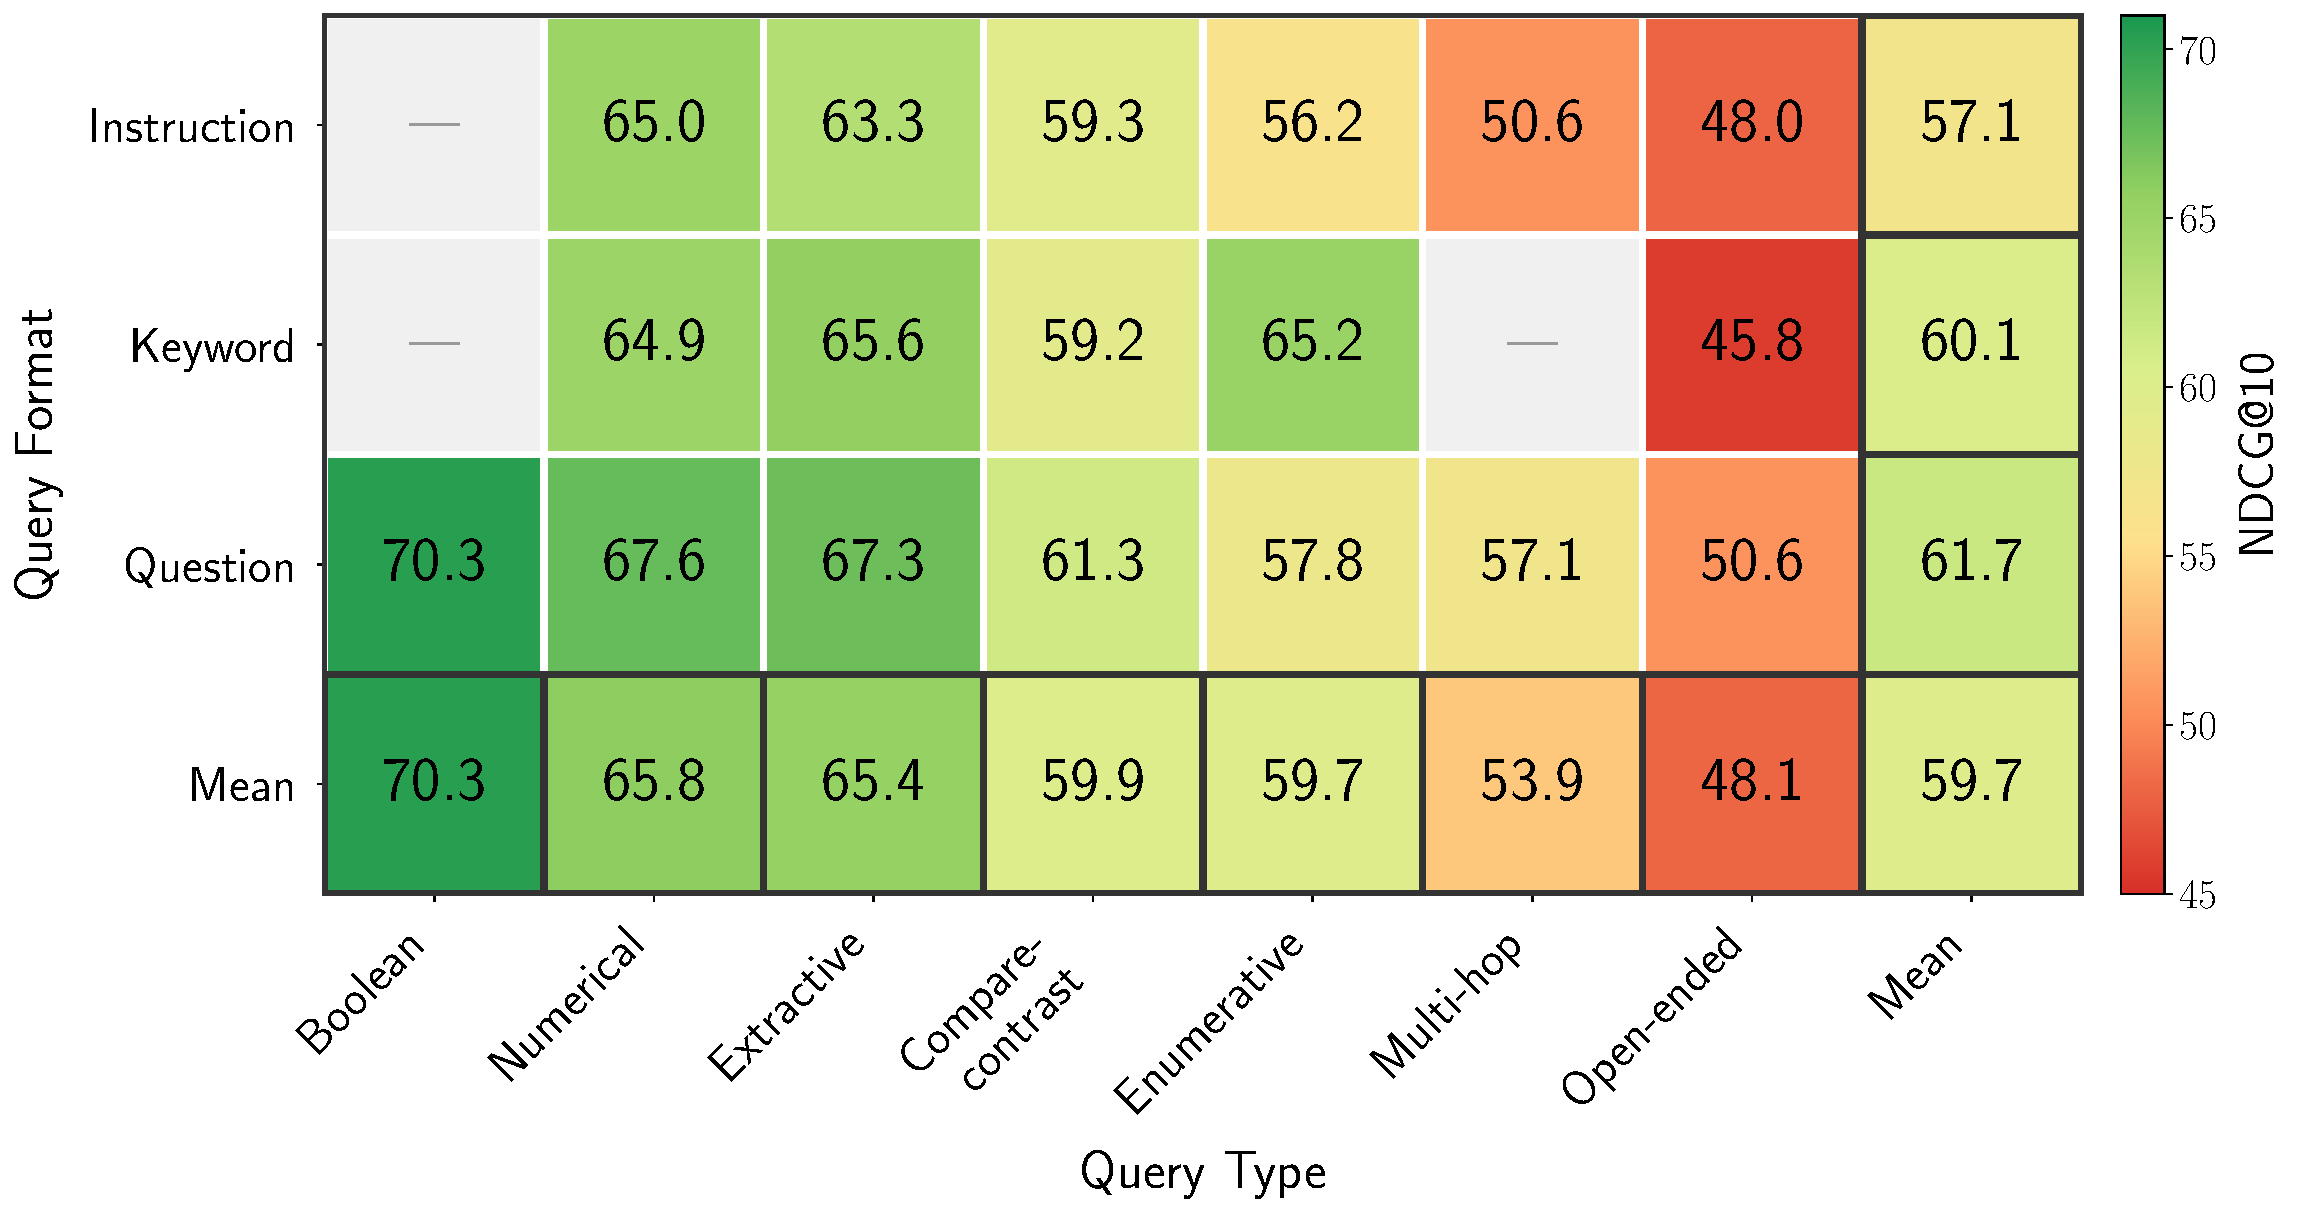
\includegraphics[width=\textwidth]{images/vidorev3_images/ndcg_by_type_format_transposed.pdf}
%         \caption{NDCG@10 by query type and format.}
%         \label{fig:ndcg_type_format}
%     \end{subfigure}
%     \hfill
%     \begin{subfigure}[t]{0.32\textwidth}
%         \centering
%         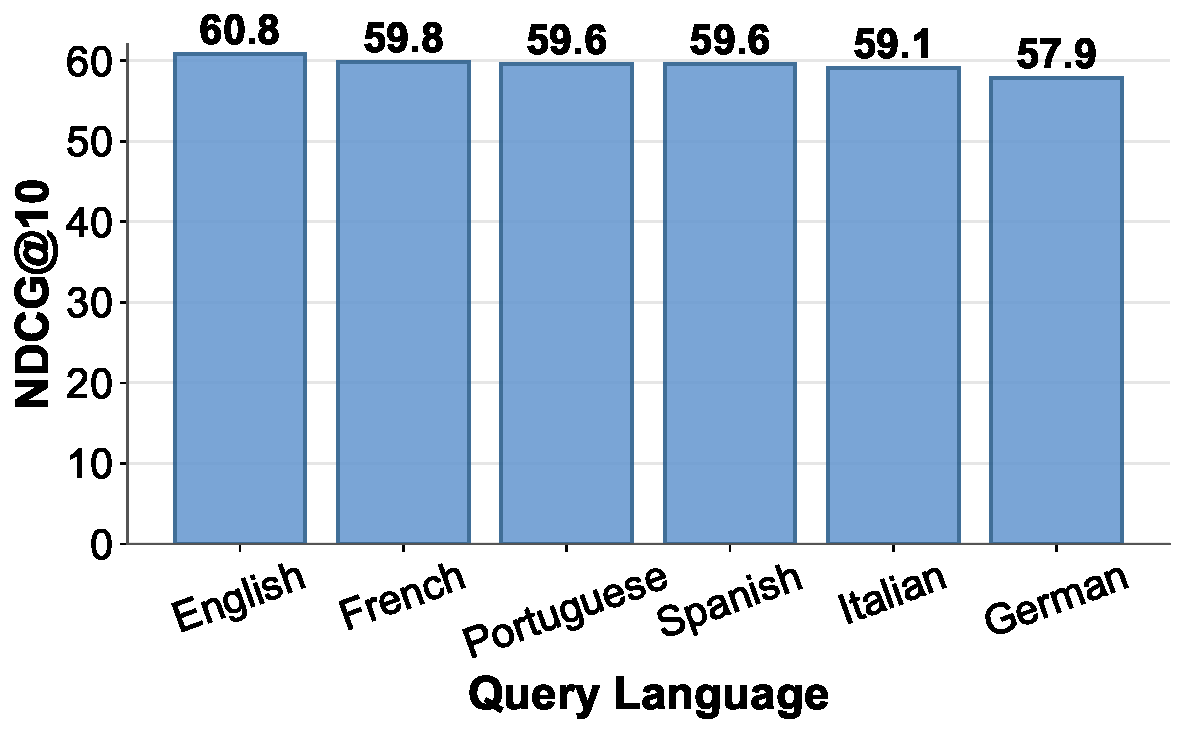
\includegraphics[width=\textwidth]{images/vidorev3_images/ndcg_by_language.pdf}
%         \caption{NDCG@10 by query language.}
%         \label{fig:ndcg_language}
%     \end{subfigure}
%     \hfill
%     \begin{subfigure}[t]{0.32\textwidth}
%         \centering
%         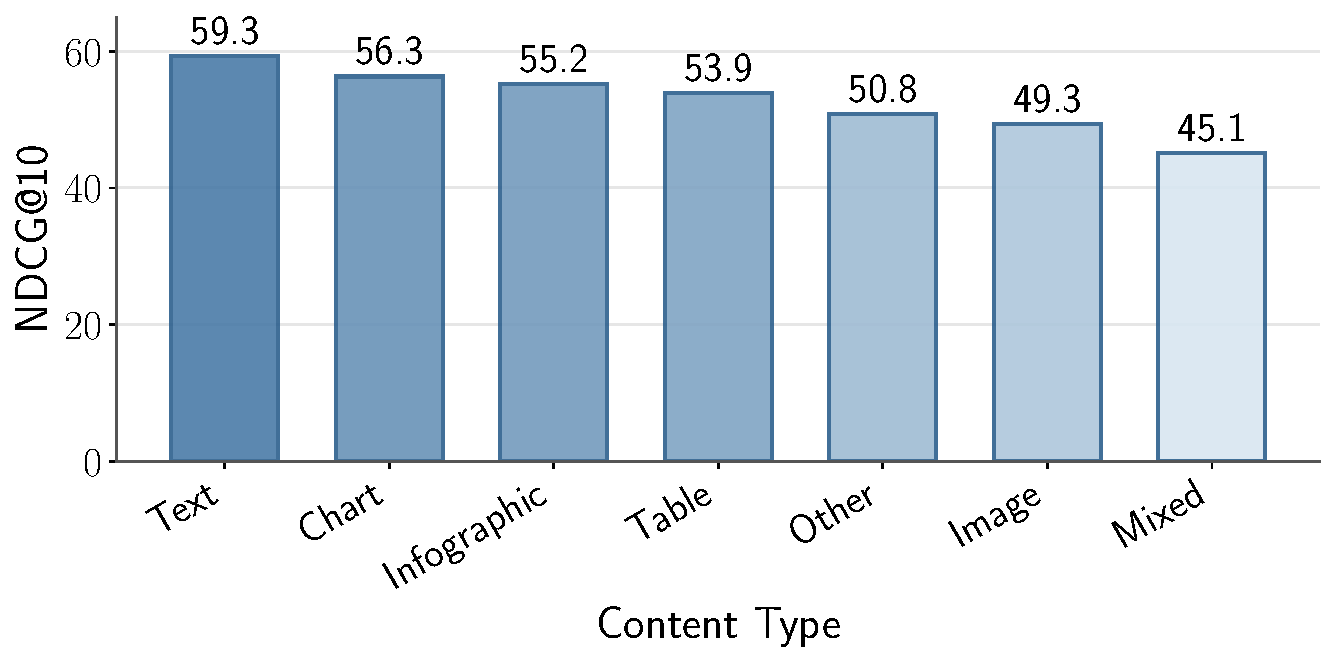
\includegraphics[width=\textwidth]{images/vidorev3_images/ndcg_by_content_type.pdf}
%         \caption{NDCG@10 by content type.}
%         \label{fig:ndcg_content}
%     \end{subfigure}
%     \caption{\textbf{ColEmbed-3B-v2 performance analysis.}}
%     \label{fig:ndcg_analysis}
% \end{figure*}
% je te laisse faire
%on vire the perf of? c'est anglais ? ok
We analyze ColEmbed-3B-v2, the best-performing retriever we evaluated across query type, content modality, and query language. % detailed results are reported in Appendix~\ref{appendix:supp retrieval}.

\paragraph{Performance is aligned with query complexity}
\Cref{fig:type-format-performance} shows that performance is inversely correlated with query complexity: simple query types such as Boolean and Numerical score significantly higher than Open-ended and Multi-hop queries. Question formulations consistently outperform Instruction and Keyword formats across nearly all categories, underscoring the need for improved handling of these query structures. %, with the notable exception of the Enumerative type for which Keyword queries score 7.4 points higher.

\begin{figure}[ht]
    \centering
    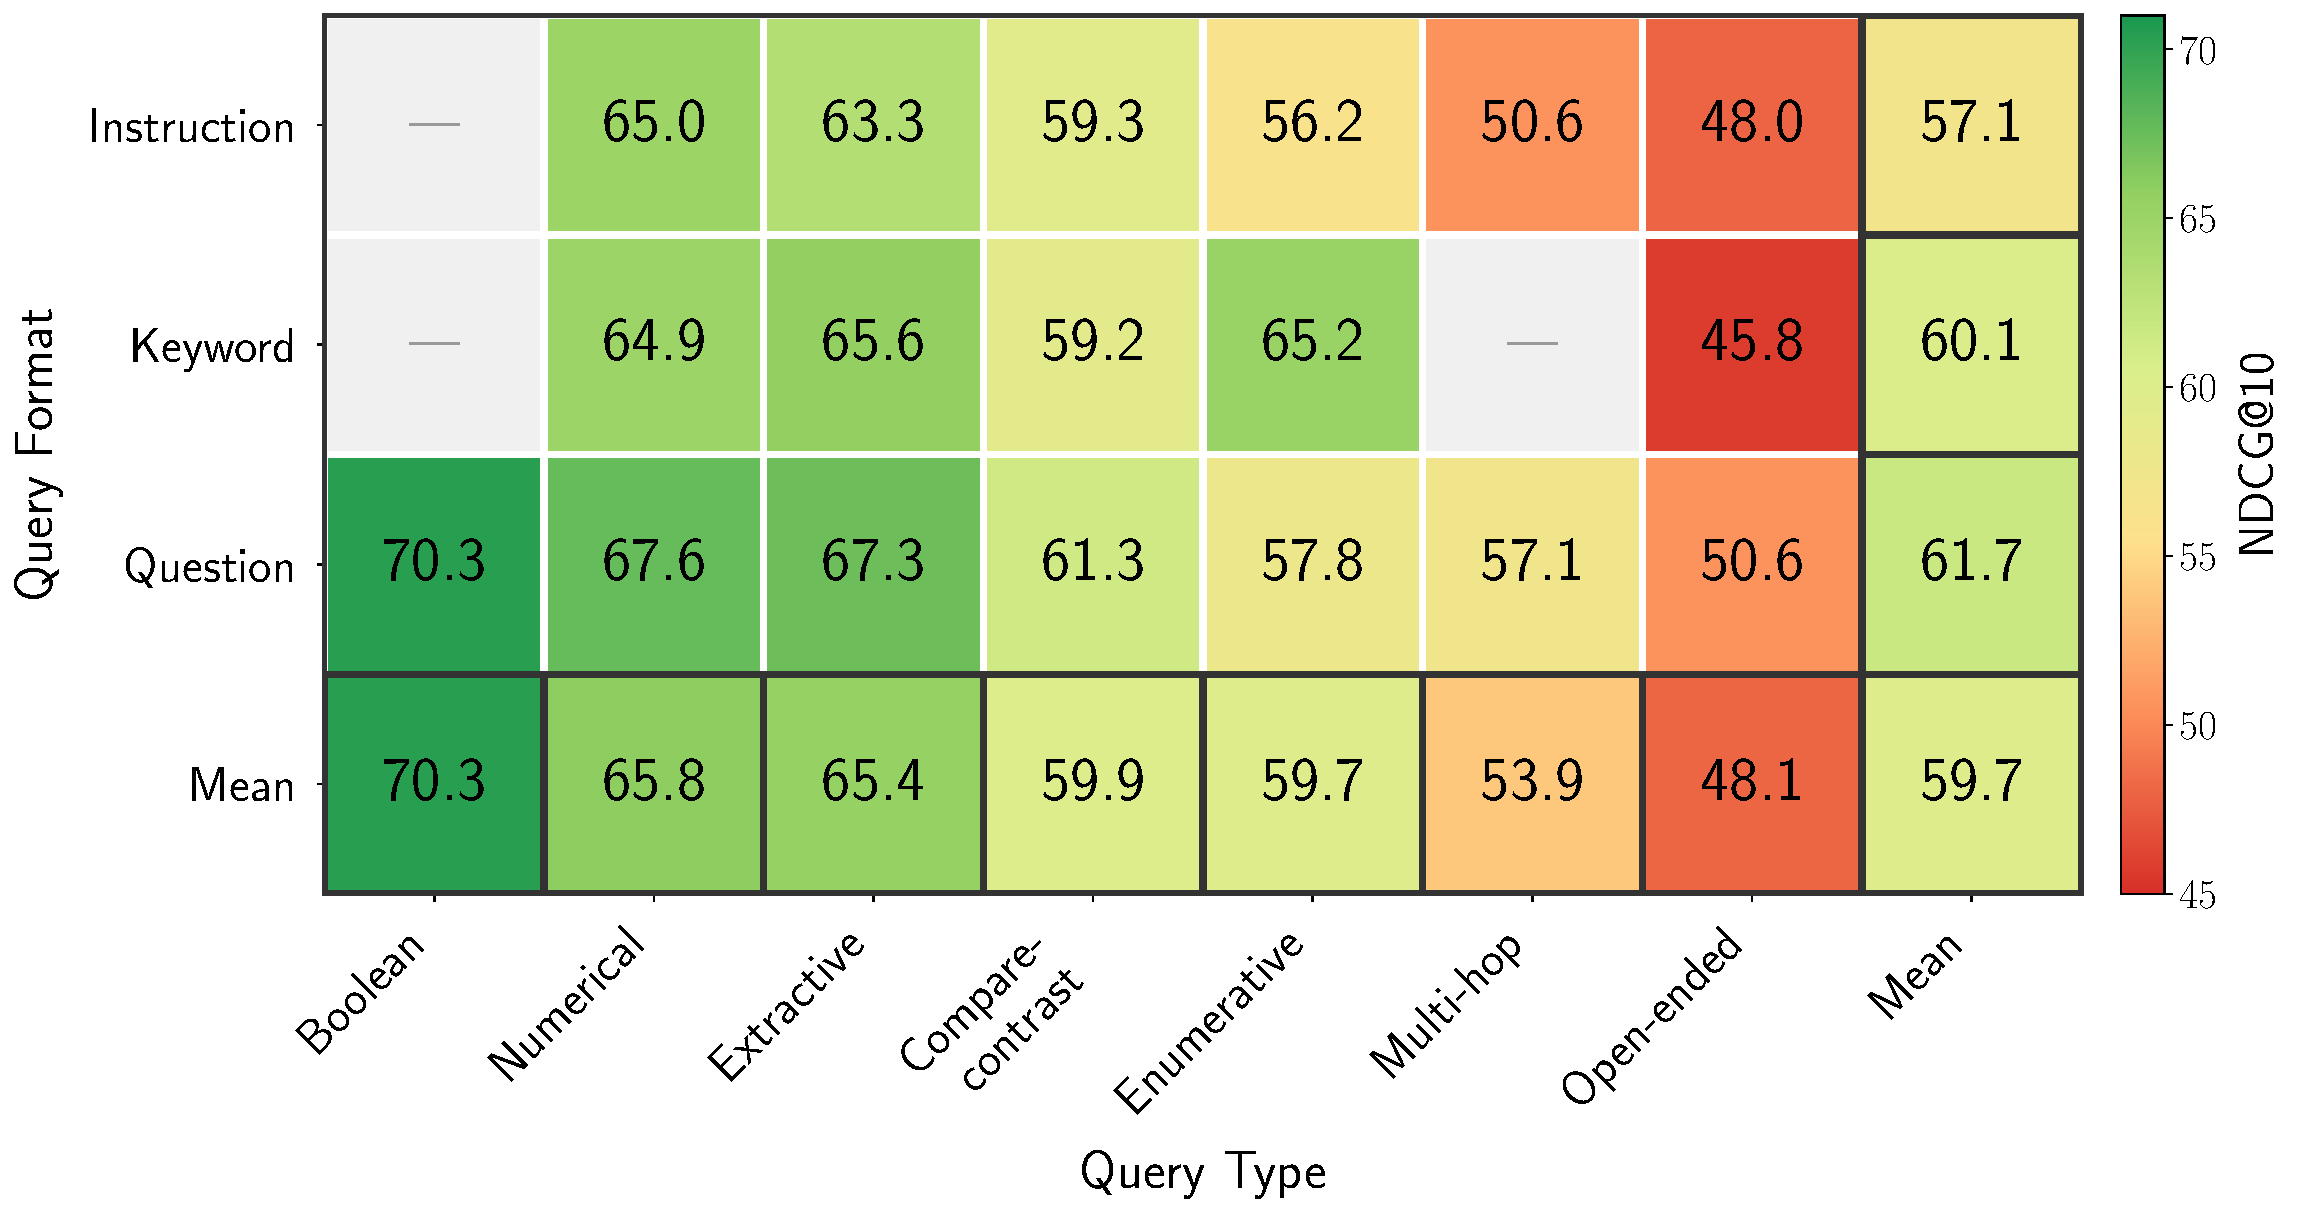
\includegraphics[width=0.99\columnwidth]{images/vidorev3_images/ndcg_by_type_format_transposed.pdf}
    \caption{\textbf{ColEmbed-3B-v2 NDCG@10 by query type and format.}}
    \label{fig:type-format-performance}
\end{figure}

% \begin{table}[h!]
% \centering
% % \resizebox{\columnwidth}{!}{%
% \begin{tabular}{lcc}
% \toprule
% Number of pages & NDCG@10 & Query count \\
% \midrule
% 1 & 76.4 & 4794 \\
% 2 & 64.7 & 3234 \\
% 3 & 60.5 & 1902 \\
% 4 & 58.7 & 1560 \\
% 5-9 & 48.5 & 4398 \\
% 10-19 & 41.2 & 2280 \\
% 20+ & 39.0 & 426 \\
% \bottomrule
% \end{tabular}
% % }
% \caption{\textbf{ColEmbed-3B-v2 NDCG@10 by number of annotated pages.}}
% \label{tab:perf number of pages}
% \end{table}

\paragraph{Visual Content and multi-page queries are hardest for retrievers}
\Cref{fig:content-type-performance} highlights that queries involving visual content like tables or images tend to be more difficult. The Mixed content type scores the lowest, which suggests that integrating information across different modalities within a single page remains a challenge. Additionally, we observe a consistent decline in performance as the number of annotated pages increases (\Cref{fig:perf number of pages}), suggesting that retriever effectiveness decreases
%when queries require aggregating information from multiple diverse sources.
when aggregating information from multiple sources is required.%\vic{think about whether this is normal for ndcg irrespective of query difficulty?} \manu{good point, not sure it's completely comparable even though ndcg is a measure of how perfect the ranking i}.

\begin{figure}[ht]
    \centering
    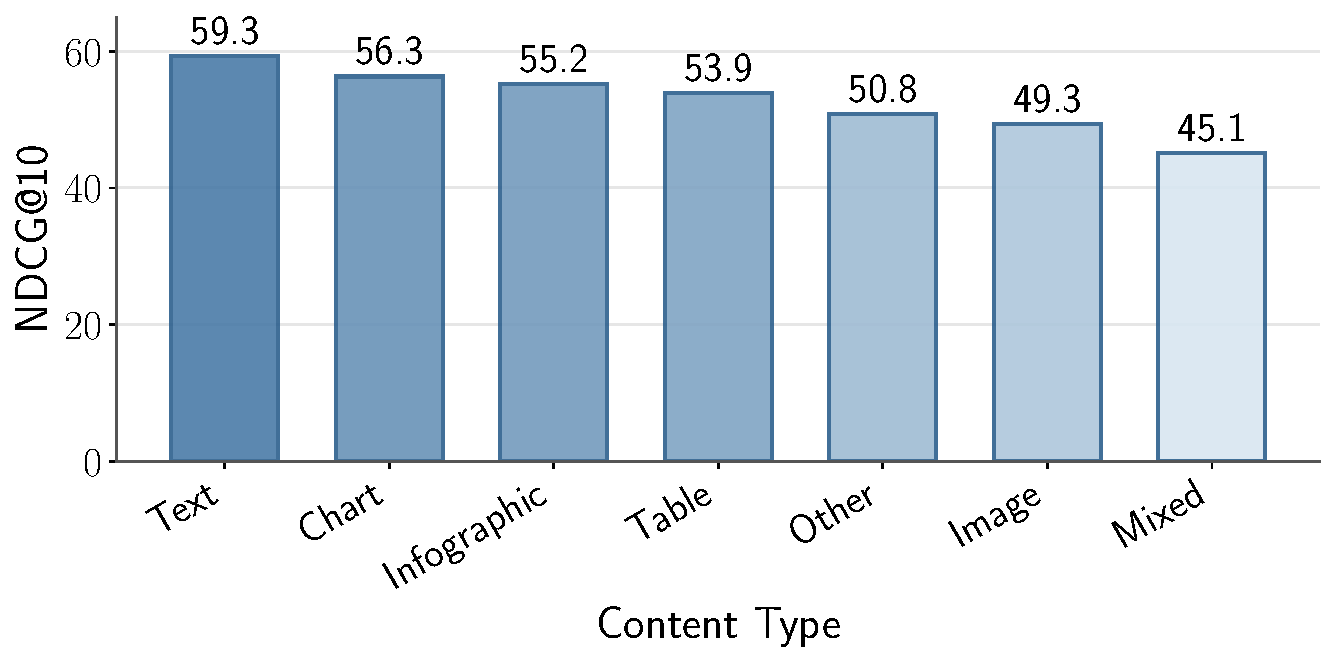
\includegraphics[width=\columnwidth]{images/vidorev3_images/ndcg_by_content_type.pdf}
    \caption{\textbf{ColEmbed-3B-v2 NDCG@10 by modality.}} 
    \label{fig:content-type-performance}
\end{figure}

\begin{figure}[h!]
    \centering
    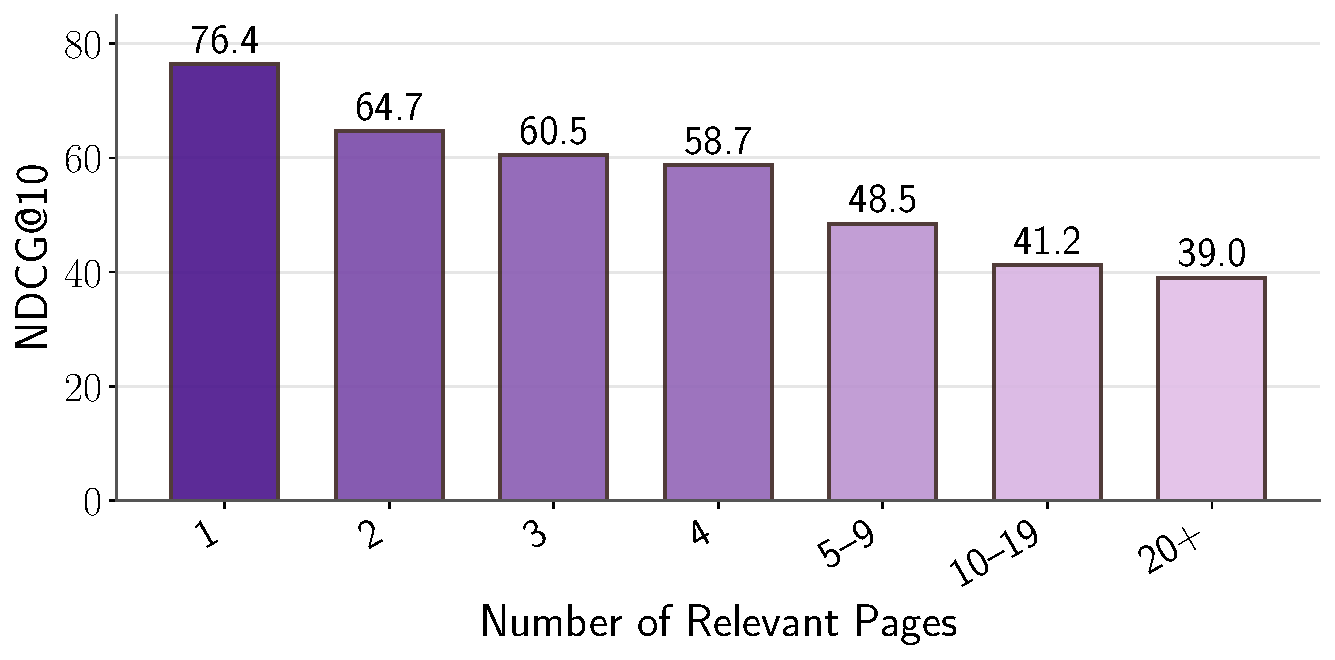
\includegraphics[width=\columnwidth]{images/vidorev3_images/ndcg_by_relevant_pages.pdf}
    \caption{\textbf{ColEmbed-3B-v2 NDCG@10 by number of annotated pages.}} 
    \label{fig:perf number of pages}
\end{figure}

\paragraph{Cross-language queries degrade performance}
Retrieval performance is 2--3 points higher in mono-lingual settings (\Cref{tab: english-only retrieval} and \Cref{tab: french-only retrieval}) than cross-lingual settings (\Cref{tab:retriever_comparison_updated}), showing that models need to better adapt to these settings. %\anto{Not super interesting}

%Retrieval performance is consistent across all 6 query languages (Table~\ref{tab:perf language}), with a 2.9 point NDCG@10 difference between the best (English, 60.8) and worst (German, 57.9) performers. However, we observe a small multilingual gap: NDCG@10 scores for English and French datasets are 2--3 points higher in a monolingual setting, where queries are in the same language as the documents (Tables~\ref{tab: english-only retrieval} and~\ref{tab: french-only retrieval}).

% \begin{figure}[ht]
%     \centering
%     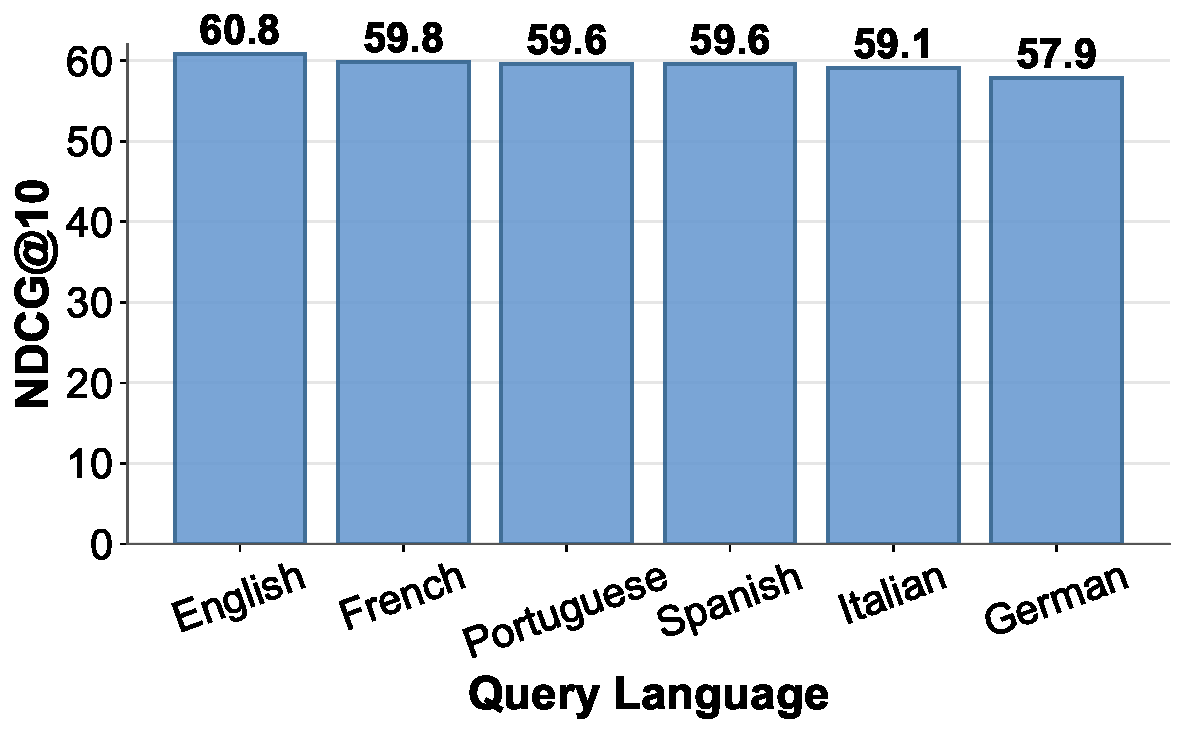
\includegraphics[width=\columnwidth]{images/vidorev3_images/ndcg_by_language.pdf}
%     \caption{ColEmbed-3B-v2 NDCG@10 by language.} 
%     \label{fig:size-performance}
% \end{figure}

\newcommand{\plus}[1]{\textcolor{teal}{\tiny \textbf{$\uparrow$#1}}}
\newcommand{\minus}[1]{\textcolor{red}{\tiny \textbf{$\downarrow$#1}}}
\newcommand{\val}[2]{\shortstack{#1 \\[-0.2em] \hspace{1.3em}#2}}
\newcommand{\dline}[2]{\shortstack{#1\\#2}}
\begin{table*}[h]
    \centering
    \small 
    \setlength{\tabcolsep}{3pt} 
    \resizebox{\textwidth}{!}{%
    \begin{tabular}{l ccccccc ccc >{\columncolor{avgcol}}c}
        \toprule
         & \multicolumn{7}{c}{\textbf{English Datasets}} & \multicolumn{3}{c}{\textbf{French Datasets}} & \multicolumn{1}{c}{} \\
        \cmidrule(lr){2-8} \cmidrule(lr){9-11}
        \textbf{Model}& \shortstack{C.S.} & \shortstack{Nucl.} & \shortstack{Fin.} & \shortstack{Phar.} & \shortstack{H.R.} & \shortstack{Ind.} & \shortstack{Tel.} & \shortstack{Phys.} & \shortstack{Ener.} & \shortstack{Fin.} & \textbf{Avg.} \\
        \midrule
        \textit{\textbf{Textual pipeline}} & \multicolumn{11}{c}{}\\
        \multirow[c]{2}{*}{\makecell[l]{Jina-v4\textsuperscript{textual} \\+ zerank-2}} &
        64.3 & 44.3 & 48.4 & 54.9 & 52.8 & 38.4 & 56.3 & 43.6 & 60.1 & 41.3 & 50.4 \\
         &
        \val{\textbf{82.1}}{\plus{17.8}} &
        \val{\textbf{53.5}}{\plus{9.2}} &
        \val{\textbf{69.2}}{\plus{20.8}} &
        \val{\textbf{66.2}}{\plus{11.3}} &
        \val{\textbf{66.5}}{\plus{13.7}} &
        \val{\textbf{53.2}}{\plus{14.8}} &
        \val{\textbf{71.5}}{\plus{15.2}} &
        \val{\textbf{48.2}}{\plus{4.6}} &
        \val{\textbf{71.5}}{\plus{11.4}} &
        \val{\textbf{53.7}}{\plus{12.4}} &
        \val{\textbf{63.6}}{\plus{13.2}} 
        \\
        \midrule
        \textit{\textbf{Visual pipeline}} & \multicolumn{11}{c}{} \\
        \multirow[c]{2}{*}{\makecell[l]{Jina-v4\textsuperscript{visual} \\+ jina-reranker-m0}} & 71.8 & 50.0 & 59.3 & 63.1 & 59.5 & 50.4 & 64.8 & 46.6 & 64.0 & 46.1 & 57.6 \\
        &
        \val{76.7}{\plus{4.9}} & 
        \val{50.8}{\plus{0.8}} & 
        \val{59.2}{\minus{0.1}} & 
        \val{65.4}{\plus{2.3}} & 
        \val{56.0}{\minus{3.5}} & 
        \val{50.9}{\plus{0.5}} & 
        \val{70.8}{\plus{6.0}} & 
        \val{46.9}{\plus{0.3}} & 
        \val{61.7}{\minus{2.3}} & 
        \val{39.8}{\minus{6.3}} & 
        \val{57.8}{\plus{0.2}} \\
        \bottomrule
    \end{tabular}
    }
    \caption{\textbf{Retrieval performance (NDCG@10) of retriever + reranker pipelines.}}
    \label{tab:reranking_scores_stacked}
\end{table*}

% \que{Condensed version but not a big fan} \paragraph{Textual rerankers help significantly; visual rerankers need improvement.} We test zerank-2 \sidecite{zeroentropy2025} and jina-reranker-m0 \sidecite{jinareranker2025} atop Jina-v4. Table~\ref{tab:reranking_scores_stacked} reveals a performance gap: though the visual base is stronger, the textual reranker yields substantial gains (+13.2 NDCG@10), outperforming the visual pipeline. Meanwhile, the visual reranker provides a marginal +0.2 average improvement and degrades performance across 4 datasets, necessitating better multilingual visual rerankers.

\paragraph{Textual rerankers outperform visual ones}

We evaluate the impact of adding a reranker to the textual and visual pipelines of the Jina-v4 retriever. We select zerank-2 \sidecite{zeroentropy2025} and jina-reranker-m0 \sidecite{jinareranker2025} as two of the leading textual and visual rerankers to date. Results in Table~\ref{tab:reranking_scores_stacked} reveal a significant disparity in reranking efficacy between modalities. While the visual retriever initially outperforms the textual base, the textual reranker yields substantial gains (+13.2 NDCG@10), enabling the textual pipeline to achieve the highest overall retrieval performance. In contrast, the visual reranker provides only a marginal average improvement of +0.2 and degrades performance in 4 datasets, underscoring the need for better multilingual visual rerankers.

%\gmor{When you evaluate with jina embedding v4 for text and image, do you use single-vector or late-interaction (as it supports both)? It is harder for cross-encoder to improve results from late interaction embedding model.}

\begin{table*}[h!]
\centering
\small
\resizebox{\textwidth}{!}{%
\begin{tabular}{l l l ccccc ccc >{\columncolor{avgcol}}c c c}
\toprule
& & & \multicolumn{5}{c}{\textbf{English Datasets}} & \multicolumn{3}{c}{\textbf{French Datasets}} & \cellcolor{white}& & \cellcolor{white} \\
\cmidrule(lr){4-8} \cmidrule(lr){9-11}
\makecell[l]{\textbf{Retrieval} \\ \textbf{pipeline}} & \makecell[l]{\textbf{Context} \\ \textbf{modality}} & \makecell[l]{\textbf{Generation} \\ \textbf{model}} & \makecell{C.S.} & \makecell{Fin.} & \makecell{Phar.} & \makecell{H.R.} & \makecell{Ind.} & \makecell{Phys.} & \makecell{Ener.} & \makecell{Fin.} & \makecell{\textbf{Avg.}\\\textbf{Hard}}& \makecell{Avg.\\Easy} & \makecell{Avg.\\Global} \\
\midrule
\multirow{3}{*}{Oracle} & Text & \multirow{3}{*}{Gemini 3 Pro} & 80.9 & 70.2 & 71.4 & \textbf{72.3} & 66.4 & 71.2 & 69.2 & 62.8 & 62.3& 79.3 & 70.6 \\
& Image & & \textbf{86.5} & \textbf{70.6} & \textbf{76.1} & 71.1 & \textbf{68.2} & 74.5 & \textbf{69.8} & \textbf{64.1} & \textbf{64.7}& \textbf{79.7} & \textbf{72.6} \\
& Hybrid & & 86.0 & 68.9 & 73.4 & 70.4 & 65.4 & 69.2 & 69.5 & 62.8 & 63.4& 77.5 & 70.7 \\
\midrule
\makecell[l]{Jina-v4\textsuperscript{text.} + zerank-2} & Text & Gemini 3 Pro & 80.9 & 66.0 & 59.9 & 63.2 & 60.4 & 69.2 & 64.9 & \underline{54.7} & 52.1& 75.5 & 64.9 \\
% \midrule
% Jina-v4\textsuperscript{text.} \& Jina-v4\textsuperscript{vis.} & Hybrid & Gemini 3 Pro & 82.8 & 62.1 & 59.6 & 61.6 & 57.2 & 64.9 & 61.4 & 51.2 & 62.6 & 71.7 & 52.2 \\
\midrule
\makecell[l]{Jina-v4\textsuperscript{text.} + zerank-2 \\ \& ColEmbed-3B-v2} & Hybrid & Gemini 3 Pro & 85.1 & 65.0 & 65.9 & 64.8 & 59.4 & 69.9 & 62.7 & 52.8 & \underline{54.7}& 76.6 & 65.7 \\
\midrule
\multirow{6}{*}{ColEmbed-3B-v2} & \multirow{2}{*}{Text} & Gemini 3 Pro & 82.3 & 62.5 & 61.0 & 62.9 & 56.2 & 64.9 & 62.3 & 49.4 & 51.7& 73.0 & 62.7 \\
 & & Kimi K2 & 81.4 & 56.6 & 59.1 & 55.7 & 55.8 & 73.8 & 60.4 & 43.1 & 44.6& 74.3 & 60.7 \\
\cmidrule{2-14}
& \multirow{4}{*}{Image} & Gemini 3 Pro & 83.3 & \underline{67.3} & 62.9 & 65.4 & 57.2 & 67.9 & 64.3 & 47.8 & 54.5& 74.1 & 64.5 \\
 & & Gemini 3 Flash & 80.9 & 64.1 & 63.5 & 63.8 & 55.1 & 68.2 & 63.3 & 47.8 & 50.3& 74.4 & 63.3 \\
& & GPT-5.2 & \underline{\textbf{86.5}} & 59.5 & \underline{68.1} & \underline{66.0} & \underline{61.5} & \underline{\textbf{76.5}} & \underline{66.2} & 49.1 & 54.1& \underline{78.1} & \underline{66.7} \\
& & Qwen3-VL-235B & 86.0 & 59.9 & 64.0 & 60.7 & 57.2 & 71.9 & 59.7 & 44.4 & 51.0& 74.1 & 63.0 \\
\bottomrule
\end{tabular}
}
\caption{\textbf{End-to-end evaluation of final answer generation.} We report the percentage of correct final answers as determined by an LLM judge across the 8 public datasets. "Oracle" rows represent the upper-bound performance using gold-standard contexts. Average Easy and Average Hard denote performance stratified by query difficulty. For each column, the best result is \textbf{bolded} and the best non-oracle result is \underline{underlined}.} % We systematically evaluate the effect of the retrieval pipeline, context modality, and generation model on the generation performance.
\label{tab:end_to_end_eval}
\end{table*}


\subsection{Final Answer Generation} \label{sec:answer results}

We evaluate end-to-end answer quality by providing LLMs and VLMs with queries and their corresponding retrieved pages, examining the effects of retrieval pipeline selection, context modality, and generation model choice (\Cref{tab:end_to_end_eval}). For this evaluation, we use the best-performing textual and visual retrieval pipelines. We additionally establish an upper bound using an \textit{oracle} pipeline that supplies the model with ground-truth annotated pages.

% For this evaluation, we use the best-performing textual and visual retrieval pipelines under 3B parameters
% -> no more reasons to say that right?

In the \textit{hybrid} configuration, we concatenate the top-5 results from the visual retriever (images) with the top-5 results from the textual retriever (text), without removing duplicates; the retrieval performance is detailed in \Cref{tab:hybrid_comparison}. We also consider a hybrid \textit{oracle} setup, which provides the model with all the ground-truth pages in both modalities.

%We evaluate the quality of final answers generated by LLMs when provided with a query and its relevant retrieved pages, assessing the impact of the retrieval pipeline, context modality, and generation model (\Cref{tab:end_to_end_eval}). We use the best-performing textual (Jina-v4) and visual (ColEmbed-3B-v2) pipelines under 3B parameters for this end-to-end evaluation. An \textit{oracle} pipeline, where the model receives the ground truth annotated pages, serves as an upper bound baseline.

The correctness of generated answers is assessed against the ground truth final answer by an LLM judge (details in Appendix \ref{appendix:final answer eval}). 
%Details on the evaluation setup are given in Appendix~\ref{appendix:final answer eval}.
Private datasets are omitted 
%from this evaluation
to maintain their integrity.

Some benchmark queries involve general knowledge manageable by LLMs without retrieval. To prevent memorization from confounding our assessment of the RAG pipeline, we stratify queries by difficulty based on parametric knowledge. A query is categorized as \textit{easy} if any model in a 6-LLM panel answers it correctly without context; otherwise, it is labeled \textit{hard}. Overall, 48.6\,\% of queries are easy (see~\Cref{tab: easy hard filtering} for details).

% A subset of queries in our benchmark can be answered by LLMs without retrieval, as they pertain to general knowledge that they already master. For these queries, high answer accuracy may reflect memorization rather than effective use of retrieved context, confounding our ability to assess the retrieval-augmented generation pipeline. To address this, we stratify queries by difficulty based on whether state-of-the-art LLMs can answer them from parametric knowledge alone. Specifically, we categorize a query as \textit{easy} if any model in a panel of 6 different LLMs answers it correctly without retrieved context; the remaining queries are labeled \textit{hard}. In total, 48.6\,\% of the queries fall into the easy category (see ~\Cref{tab: easy hard filtering} for a breakdown by dataset and panel model).

\paragraph{Visual context helps generation} With a fixed Gemini 3 Pro generator, image-based context outperforms text-based context on the hard subset by 2.4 and 2.8 percentage points for the oracle and ColEmbed-3B-v2 pipelines, respectively (\Cref{tab:end_to_end_eval}). This confirms that preserving the visual content of document pages provides better grounding for complex answer generation.

% \manu{check bold takeaway formatting}

%\paragraph{Generation quality reflects retrieval performance} Performance differences between retrieval pipelines persist in final answer quality. Notably, a strong textual pipeline (jina-embeddings-v4+zerank-2) can match a visual pipeline (colembed-3b-v2), achieving 64.9\% versus 64.5\% accuracy \que{TODO : rather talk about hard subset}. 
% \gmor{We might add a comment that for hard questions visual retrieval with ColEmbed-3B-v2 is better (54.5) than Jina text embedding+reranker pipeline (52.2)} 
%The 6 percentage point gap between oracle and the best retrieval pipelines highlights the effect of retrieval errors on final answer quality. % TODO: Rework this paragraph. The message is not well supported

\paragraph{Hybrid retrieval yields the best performance on challenging queries} The hybrid pipeline achieves 54.7\,\% accuracy on hard queries, surpassing both the strongest textual (52.1\,\%) and visual (54.5\,\%) baselines. This complementary effect suggests that text and image representations capture different aspects of document content, and their combination can provide more robust evidence for downstream generation. %\que{Not sure about last sentence, seems difficult to back} Conversely, the hybrid oracle (63.4\,\%) trails the image-only upper bound (64.7\,\%), indicating that the redundancy beneficial for retrieval robustness effectively dilutes the signal compared to pure visual grounding.

\paragraph{Hard queries expose the limits of parametric knowledge in current models} Even with oracle context, performance on hard queries lags behind easy queries by more than 10 percentage points. This gap suggests that the multi-step reasoning and long-context synthesis required for difficult queries remain challenging for current models. While the models we evaluate achieve comparable overall scores, their relative ranking may shift when parametric knowledge is less of an advantage, as shown by GPT 5.2 outperforming Gemini 3 Pro on easy queries but trailing on hard ones.

%\paragraph{Query difficulty is the main driver of performance variation} \anto{Don't like this sentence} Even with oracle context, performance on hard queries lags behind easy queries by more than 10 percentage points. This gap suggests that the multi-step reasoning and long-context synthesis required for difficult queries remain challenging for current models. While the models we evaluate achieve comparable overall scores, their relative ranking may shift when parametric knowledge is less of an advantage, as shown by GPT 5.2 outperforming Gemini 3 Pro on easy queries but trailing on hard ones.

\paragraph{ViDoRe V3 leaves significant room for future retriever improvements} The 10-point gap between the best non-oracle result (54.7\,\%) and the image oracle (64.7\,\%) on hard queries underscores substantial opportunities for improving the retrieval pipeline. Moreover, even with oracle contexts, Gemini 3 Pro performance remains modest, indicating that generation models still struggle to fully exploit the provided information.

%\paragraph{Generation quality reflects retrieval performance} \aedy{either change name or takeaway} Performance differences between retrieval pipelines persist in final answer quality. While the best textual (jina-embeddings-v4+zerank-2) and visual (colembed-3b-v2) pipelines show comparable overall averages, a distinct advantage for visual retrieval emerges on the hard subset (+2.4\,\%). The significant 10-point gap between the best non-oracle result (54.7\,\%) and the image oracle (64.7\,\%) on hard queries highlights the substantial room for improvement in retrieval pipelines.


% \begin{table*}[h]
% \centering
% \label{tab:ragchecker_metrics}
% \resizebox{\textwidth}{!}{%
% \begin{tabular}{l|ccc|cc|cccccc}
%  & \multicolumn{3}{c}{\textit{Overall}} & \multicolumn{2}{c}{\textit{Retriever}} & \multicolumn{6}{c}{\textit{Generator}} \\
% \midrule
% Domaine & Precision $\uparrow$ & Recall $\uparrow$ & F1 $\uparrow$ & \dline{Claim}{Recall} $\uparrow$ & \dline{Context}{Precision} $\uparrow$ & \dline{Context}{Utilisation} $\uparrow$ & \dline{Noise}{Sensitivity (R)} $\downarrow$& \dline{Noise}{Sensitivity (I)} $\downarrow$ & Hallu. $\downarrow$ & \dline{Self}{Knowledge} $\downarrow$ & Faith. $\uparrow$\\
% \midrule
% Computer Science & 70.9 & 68.2 & 60.2 & 89.9 & 85.0 & 70.7 & 18.1 & 1.4 & 9.6 & 4.0 & 86.3 \\
% Energy (FR) & 62.6 & 65.6 & 55.1 & 81.2 & 75.7 & 66.6 & 20.2 & 4.7 & 12.5 & 5.7 & 81.9 \\
% Finance (EN) & 63.8 & 52.7 & 47.9 & 85.8 & 71.3 & 52.0 & 17.2 & 5.1 & 13.9 & 5.3 & 80.9 \\
% Finance (FR) & 51.3 & 55.5 & 43.0 & 76.9 & 68.3 & 54.2 & 25.3 & 7.1 & 16.4 & 5.8 & 77.8 \\
% HR (EN) & 65.5 & 56.7 & 50.7 & 80.9 & 66.2 & 55.3 & 18.1 & 3.8 & 12.6 & 6.5 & 80.9 \\
% Industrial (EN) & 63.7 & 58.2 & 49.6 & 85.4 & 76.4 & 59.3 & 20.7 & 4.7 & 11.0 & 5.9 & 83.2 \\
% Pharmaceuticals (EN) & 62.5 & 65.8 & 55.1 & 82.2 & 73.6 & 64.7 & 19.8 & 3.4 & 14.2 & 9.7 & 76.0 \\
% Physics (FR) & 63.2 & 65.8 & 55.0 & 74.0 & 74.0 & 68.1 & 14.8 & 2.7 & 19.2 & 13.4 & 67.4 \\
% \midrule
% Mean & 62.9 & 61.1 & 52.1 & 82.0 & 73.8 & 61.4 & 19.3 & 4.1 & 13.7 & 7.0 & 79.3 \\
% \midrule
% Easy queries & 63.6 & 65.6 & 53.8 & 86.0 & 76.9 & 66.2 & 21.2 & 2.8 & 12.4 & 6.8 & 80.8 \\
% Hard queries & 62.0 & 55.8 & 49.6 & 79.1 & 71.1 & 55.7 & 18.1 & 5.2 & 14.7 & 6.8 & 78.4 \\
% \bottomrule
% \end{tabular}%
% }
% \caption{RAGChecker Metrics across Datasets, for Oracle retriever + gpt-5 \aedy{wdyt}\\ \aedy{METRICS: https://github.com/amazon-science/RAGChecker}}
% \end{table*}

\subsection{Visual Grounding} \label{sec:visual grounding results}

Beyond generating correct answers, it is highly desirable for RAG pipelines to identify where in the source documents the answer originates, enabling users to verify the grounding of the query answer. We therefore evaluate the ability of LLMs to generate accurate bounding boxes within their final answer. Among the few LLM families with visual grounding capabilities, we select Qwen3-VL-30B-A3B-Instruct and Gemini 3 Pro for evaluation. For each query, we provide the model with the candidate pages shown to the human annotators and prompt it to answer the query while inserting inline bounding boxes in XML format \texttt{<bboxes image="N"> ... </bboxes>} to delimit relevant content (full instructions in Appendix~\ref{appendix: bbox}).

We use the bounding boxes produced by the human annotators as our ground truth. Since each query may have 1--3 human annotators, we evaluate VLM predictions independently against each annotator using the same zone-based methodology as the inter-annotator consistency analysis (Section~\ref{sec: grounded qa}), and report the highest F1 score. This best-match strategy reflects the inherent subjectivity of evidence selection: annotators may legitimately highlight different regions to support the same answer, and a model should not be penalized for matching any valid interpretation.

% \begin{table}[h!]
% \centering
% \footnotesize
% \setlength{\tabcolsep}{6pt}
% \begin{tabular}{@{}lc@{}}
% \toprule
% Predictor & F1 \\
% \midrule
% Qwen3-VL-30B-A3B & 0.089 \\
% Gemini 3 Pro & 0.065 \\
% \addlinespace[0.2em]
% \textit{Human Agreement} & \textit{0.602} \\
% \bottomrule
% \end{tabular}
% \caption{Average Localization F1 scores.}
% \label{tab:bbox_f1}
% \end{table}

\paragraph{Visual grounding lags human performance} 
Inter-annotator agreement on evidence localization reaches an F1 of 0.602, whereas the best-performing models achieve markedly lower scores: 0.089 for Qwen3-VL-30B-A3B-Instruct and 0.065 for Gemini 3 Pro. A page-level analysis (\Cref{tab:bbox_consistency_comparison}) reveals that on pages where humans provided bounding boxes, both models annotated the same page only 16--17\,\% of the time, while 26--27\,\% of human-annotated pages received no model annotation at all—highlighting recall as the primary bottleneck. Detailed per-domain results and qualitative analysis appear in Appendix \ref{appendix: bbox} and \ref{appendix: bbox examples}.

%Table~\ref{tab:bbox_consistency_comparison} provides a page-level analysis of annotation presence: on pages where humans provided bounding boxes, both models annotated the same page only 16--17\,\% of the time, while 26--27\,\% of human-annotated pages received no model annotation at all, highlighting recall as the primary limitation. Localization F1 scores (Figure~\ref{fig:bbox evaluation}) reveal that the models score substantially below inter-annotator agreement (Table~\ref{tab:inter-annotator bbox agreement}). Qualitative analysis reveals distinct failure modes (examples in Appendix~\ref{appendix: bbox examples}). Gemini frequently produces off-by-one page indexing errors: the predicted coordinates would correctly localize the target content if applied to an adjacent page. The two models also differ in box granularity: Gemini tends to draw tight boxes around individual elements (e.g., a single table cell or text line), whereas Qwen3-VL generates larger boxes encompassing entire sections or paragraphs, more closely matching human annotation patterns \gmor{If we need to save some space for submission, these details about how Gemini and Qwen3-VL generates boxes could go to the Appendix}. This difference partially explains Qwen3-VL's higher F1 scores, as broader boxes are more likely to overlap with the ground-truth zones used in our evaluation.

% \paragraph{Agreement-Based Stratification}
% To understand how VLM performance varies with annotation ambiguity, we stratify results by inter-annotator agreement level. For multi-annotator samples, we compute pairwise zone IoU between all annotator pairs and classify agreement as \textit{high} (mean pairwise IoU $\geq 0.7$), \textit{medium} ($0.3 \leq$ IoU $< 0.7$), \textit{low} (IoU $< 0.3$), or \textit{single} (one annotator only).


% \begin{table*}[h!]
% \centering
% \small 
% \setlength{\tabcolsep}{3pt} 
% % \resizebox{\textwidth}{!}{%
% \begin{tabular}{l ccccccc ccc c} % Removed columncolor from here
% \toprule
%  & \multicolumn{7}{c}{\textbf{English Datasets}} & \multicolumn{3}{c}{\textbf{French Datasets}} & \\ % This cell is now white
% \cmidrule(lr){2-8} \cmidrule(lr){9-11}
% \makecell[l]{\textbf{Model}} & \makecell{C.S.} & \makecell{Nucl.} & \makecell{Fin.} & \makecell{Phar.} & \makecell{H.R.} & \makecell{Ind.} & \makecell{Tel.} & \makecell{Phys.} & \makecell{Ener.} & \makecell{Fin.} & \makecell{\textbf{Average}} \\
% \midrule
% Qwen3-VL-30B-A3B & 0.058 & 0.094 & 0.050 & 0.157 & 0.054 & 0.066 & 0.078 & 0.198 & 0.086 & 0.044 & \cellcolor{avgcol}\textbf{0.084} \\
% Gemini 3 Pro & 0.055 & 0.070 & 0.036 & 0.103 & 0.036 & 0.035 & 0.073 & 0.144 & 0.067 & 0.028 & \cellcolor{avgcol}\textbf{0.061} \\
% \bottomrule
% \end{tabular}
% %}
% \caption{\textbf{Model bounding box localization performance}. Each F1 score measures the zone-based overlap between model-generated bounding boxes and human annotations, using the annotator yielding the highest F1.\vic{Transform into graph to make this more legible?}}
% \label{tab:bbox evaluation}
% \end{table*}


\begin{table}[h!]
\centering
\resizebox{\columnwidth}{!}{%
\begin{tabular}{llcc}
\toprule
\textbf{Category} & \textbf{Outcome} & \textbf{Qwen3-VL-30B-A3B} & \textbf{Gemini 3 Pro} \\
\midrule
\multirow{2}{*}{\textbf{Agreement}} 
  & Both annotated & 17\,\% & 16\,\% \\
  & Neither annotated  & 46\,\% & 49\,\% \\
\addlinespace
\multirow{2}{*}{\textbf{Discrepancy}} 
  & Model only   & 10\,\% & 7\,\% \\
  & Human only & 26\,\% & 27\,\% \\
\bottomrule
\end{tabular}
}
\caption{\textbf{Page-level bounding box agreement between models and human annotators.} Each page is classified by whether the model and human both annotated it, both left it unannotated, or only one provided annotations.}
\label{tab:bbox_consistency_comparison}
\end{table}



% \begin{table}[h!]
% \small
% \centering
% \resizebox{\columnwidth}{!}{%
% \begin{tabular}{lc}
% \toprule
% \textbf{Predictor} & \textbf{F1} \\
% \midrule
% Qwen3-VL-30B-A3B & 0.089 \\
% Gemini 3 Pro & 0.065 \\
% \hline
% Human & 0.602 \\
% \bottomrule
% \end{tabular}
% }
% \caption{\textbf{Average Localization F1 score over each corpus.}}
% \label{tab:bbox_f1}
% \end{table}


% \paragraph{Visual Document Understanding (VDU)} The field of VDU has traditionally relied on datasets such as DocVQA \sidecite{mathew_docvqa_2020} and CharXiv \sidecite{wang2024charxiv}. Such works are also often specialized in one particular document type \sidecite{mathew2021infographicvqa, zhu_towards_2022, tanaka2023slidevqa} While these benchmarks have been instrumental in advancing multimodal understanding, they are primarily designed for single-page or single-image tasks. They do not require the system to sift through large corpora, thereby bypassing the retrieval challenges inherent in RAG. Furthermore, recent efforts to introduce bounding box supervision, such as BBox-DocVQA \sidecite{yu2025bboxdocvqalargescale}, remain restricted to these single-page contexts and do not address multi-page retrieval scenarios.

% \paragraph{Retrieval-Centric Benchmarks} The rapid evolution of visual retrieval models \sidecite{yu2024visragvisionbasedretrievalaugmentedgeneration, ma2024unifyingmultimodalretrievaldocument}, particularly ColBERT style late-interaction architectures like ColPali \sidecite{faysse2025colpaliefficientdocumentretrieval, xu2025llamanemoretrievercolembedtopperforming}, has necessitated new evaluation frameworks. Benchmarks such as Jina-VDR \sidecite{günther2025jinaembeddingsv4universalembeddingsmultimodal} and ViDoRe V1/V2 \sidecite{faysse2025colpaliefficientdocumentretrieval, macé2025vidorebenchmarkv2raising} have been developed to measure retrieval precision. However, these benchmarks largely isolate the retrieval step. They overlook the subsequent generation phase, failing to evaluate whether the retrieved context is sufficient for a model to synthesize a coherent, grounded answer.

% \paragraph{End-to-End Multimodal RAG}
% While textual RAG benchmarks have recently evolved to capture realistic, non-trivial user needs \sidecite{thakur2025freshstackbuildingrealisticbenchmarks, tang2024multihopragbenchmarkingretrievalaugmentedgeneration, su2024bright}, this level of query complexity remains largely underexplored for multimodal RAG. In contrast, multimodal RAG evaluation still lacks this depth \sidecite{faysse2025colpaliefficientdocumentretrieval, wang2025vidorag, wasserman2025real}.Recent works like DUDE \sidecite{van2023document} and M3DocRAG \sidecite{cho2024m3docrag} extend evaluation to multi-page settings but remain heavily skewed toward extractive tasks. These datasets typically demand short, factoid answers that do not stress the multi-step reasoning or synthesis capabilities required by open-ended enterprise queries.The closest contemporary work, UniDocBench \sidecite{peng2025unidocbenchunifiedbenchmarkdocumentcentric}, offers a significant step toward end-to-end evaluation with tasks including summarization and reasoning. However, it relies heavily on synthetic generation with sparse human verification, is limited to a single language, and lacks the fine-grained visual grounding annotations necessary to diagnose hallucinations in complex layouts. Our work bridges these gaps by providing a multilingual, expert-verified benchmark that enforces visual grounding and targets complex, open-ended reasoning.

% \manu{Not sure this RW brings a lot compared to what is in the intro. Maybe call the intro "intro and Related Work" and add a few citations there. It seems quite redundant here.}

\section{Conclusion}

This work introduces ViDoRe V3, a multilingual, human-annotated RAG benchmark that evaluates retrieval, final answer generation, and visual grounding on large industry-relevant document corpora. We design a human-in-the-loop annotation methodology, deployed in a 12,000-hour annotation campaign, that produces diverse realistic queries paired with relevant pages, bounding boxes, and reference answers. Evaluating state-of-the-art RAG pipelines, we find that visual retrievers outperform textual ones, late interaction and textual reranking yield substantial gains, and visual context improves answer generation quality. Looking ahead, ViDoRe V3 highlights several concrete research directions for practical multimodal RAG. Retriever models still struggle on cross-lingual and open-ended queries requiring visual interpretation, while VLMs need improvement in answer generation from multi-page contexts as well as accurate visual grounding. By providing a rigorous framework for evaluating these limitations, ViDoRe V3 serves as a catalyst for the development of more robust, intelligent document understanding models.

% \setchapterpreamble[u]{\margintoc}
\chapter{ModernVBERT: Towards Smaller Visual Document Retrievers}
\label{ch:modernvbert}



\def\flagship{\emph{ModernVBERT}}
\def\flagshipbase{\flagship-base}
\def\flagshipembed{\flagship-embed}
\def\biflagship{\emph{BiModernVBERT}}
\def\colflagship{\emph{ColModernVBERT}}
\def\flagshipparameters{250M}

\newcommand{\cmark}{\ding{51}}% checkmark
\newcommand{\xmark}{\ding{55}}% crossmark

\def\natcap{\textit{NatCap}}
\def\repo{\url{https://huggingface.co/ModernVBERT}}
\def\ghrepo{\url{https://github.com/illuin-tech/modernvbert}}

% Preamble additions:
% \usepackage{booktabs, multirow, makecell, rotating, xcolor, colortbl}
% \usepackage[flushleft]{threeparttable}
\renewcommand\theadfont{\bfseries}
% Define custom colors
\definecolor{grpA}{HTML}{E8F4FF}     % paler blue for group banners
\definecolor{grpB}{HTML}{FFE8EB}     % paler pink for group banners
\definecolor{grpC}{HTML}{E8FFEF}     % paler mint for group banners
\definecolor{grpD}{HTML}{FFF0E0} 
\definecolor{grpE}{HTML}{FFF0F6} 
\definecolor{avgcol}{gray}{0.9}      % avg column grey
\definecolor{dscol}{gray}{0.95}      % dataset name column background
\definecolor{latcol}{RGB}{210,235,255} % light blue for latency column
\definecolor{latcpucol}{RGB}{210,235,255} % light blue (CPU)
\definecolor{latgpucol}{RGB}{170,215,255} % slightly darker blue (GPU)


\begin{sagekaobox}[frametitle=Paper Context]
After the release of ColPali, many Visual Document Retrieval models were trained by various academic and industrial teams around the world, including from our team. Most efforts centered around leveraging stronger VLM backbones which we have shown with the \emph{ColQwen} series to directly improve retrieval performance. 
In this paper released in September 2025 and published at ICML 2026, we instead take another route. With ModernVBERT, we maintain ColPali retrieval performance with a model 10 times smaller. Beyond the ressource release, this paper should be seen as a thorough exploration of the performance factors behind repurposing VLMs for visual embeddings. Our ablations span architecture research, data mixes, cross-modality positive transfers, model souping and more. Importantly, we show strong retrieval performance can be achieved even with little ressources at querying time, enabling cheap deployments and widespread industrial use of the VDR technology.
\end{sagekaobox}


\begin{kaobox}[frametitle=Paper Abstract]
Retrieving specific information from a large corpus of documents is a prevalent industrial use case of modern AI, notably due to the popularity of Retrieval-Augmented Generation (RAG) systems. Although neural document retrieval models have historically operated exclusively in the text space, Visual Document Retrieval (VDR) models - large vision-language decoders repurposed as embedding models which directly work with page screenshots as inputs - are increasingly popular due to the performance and indexing latency gains they offer. In this work, we show that, while cost-efficient, this approach of repurposing generative models bottlenecks retrieval performance. Through controlled experiments, we revisit the entire training pipeline, and establish a principled recipe for improving visual document retrieval models. We notably measure the impact of attention masking, image resolution, modality alignment data regimes, and late interaction centered contrastive objectives which emerge as central performance factors. Building on these insights, we release ModernVBERT, a compact 250M-parameter vision-language encoder that outperforms recent models up to 10 times larger when fine-tuned on document retrieval tasks, enabling efficient inference on cheap CPU hardware and greatly reducing latency and costs while maintaining strong performance. Models, code and data are available at \repo.

\end{kaobox}


\section{Introduction}\label{sec:intro}



\begin{figure}[t]
  \centering
  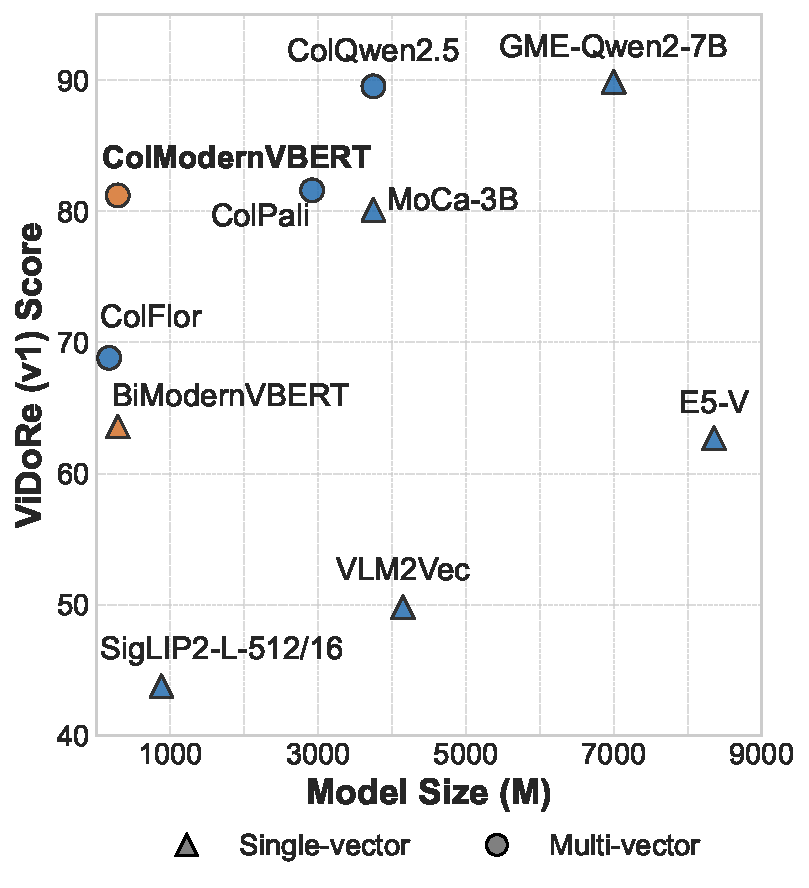
\includegraphics[width=0.88\linewidth]{images/modernvbert_figures/fig_1/pareto_large_models_ColModernVBERT_orange.pdf}
  \caption[Pareto efficiency]{\textbf{Pareto efficiency.} \colflagship{} outperforms models in its category on ViDoRe, achieving a leading performance-size tradeoff.}
  \label{fig:pareto_vidore}
  %\vspace{-10pt}                         % tighten bottom spacing (tweak as needed)
\end{figure}

% Context paragraph
% this is colpali's first paragraph, nice start point but to be modified. I think the reviewer is right in the sense that let's not overcomplicate the first paragraph. in the end its VDR so let's simply motivate it. @manu, c'est un draft fais toi plaisir, jen suis pas 100% convaincu de la forme mais j'aime le fond
% \textcolor{red}{Visual Document Retrieval (VDR) is a recently introduced alternative to text-based search systems, which, given a user query, consists in identifying relevant document pages within a large corpus by relying on their image screenshots rather than their pre-extracted textual content \sidecite{faysse2025colpaliefficientdocumentretrieval}. 
%Applications of Retrieval Augmented Generation (RAG) \sidecite{lewis_retrieval-augmented_2020} are ubiquitous in the industry, but remain bottlenecked by the quality of the first-stage retrieval system. To process documents such as PDFs, for many years, the standard approach was to extract the textual information of the documents--relying on OCR modules--and perform retrieval in the text space \sidecite{lin-byrne-2022-retrieval}.} Owing to the performance improvements enabled by generative vision–language models (VLMs), recent work has increasingly explored \textcolor{red}{operating in the vision space instead}, repurposing these models as multimodal encoders through extended contrastive post-training~\sidecite{ma2024unifyingmultimodalretrievaldocument, faysse2025colpaliefficientdocumentretrieval, jiang2024vlm2vectrainingvisionlanguagemodels}.

The ability to quickly locate specific information in vast document collections is a core building block of digital systems today, supporting use cases that range from web search and virtual assistants to enterprise knowledge management. Neural information retrieval (IR) models, and in particular dense retrievers, have become the de facto backbone of modern search systems thanks to their strong semantic matching capabilities and good scalability properties \sidecite{reimers2019sbert, karpukhin2020dpr, wang_text_2022}.  

This trend is amplified by the widespread adoption of Retrieval-Augmented Generation (RAG) \sidecite{lewis_retrieval-augmented_2020}, where a retriever is used to select a small set of relevant documents that condition a downstream generator. In such systems, the first-stage retrieval module is a well-known bottleneck: its recall directly upper-bounds the quality of the generated answers, while its latency and indexing costs partially drive the overall system efficiency \sidecite{lin-byrne-2022-retrieval}. As a result, improving document retrieval, especially for long, complex files such as PDFs, scientific articles, and reports, is a key lever for making industrial RAG deployments more accurate and cost-effective.
% \begin{wrapfigure}[24]{tr}{0.52\textwidth} % <- 12 = approx. number of text lines to wrap
%   \vspace{-5pt}                          % tighten top spacing (tweak as needed)
%   \centering
%   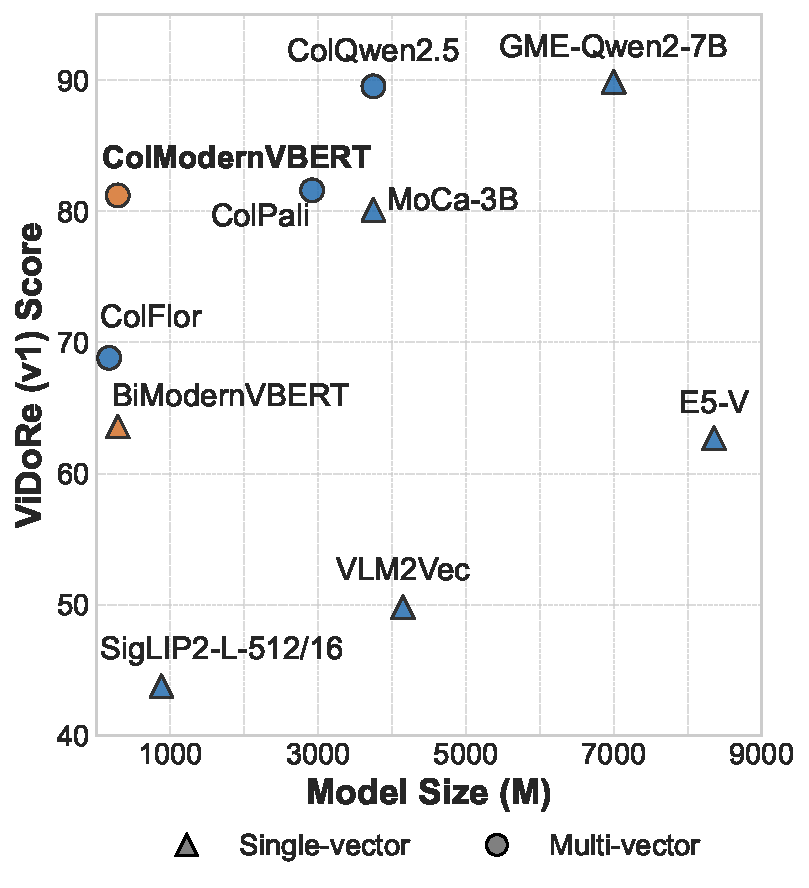
\includegraphics[width=\linewidth]{images/modernvbert_figures/fig_1/pareto_large_models_ColModernVBERT_orange.pdf}
%   \caption{\textbf{Pareto efficiency.} \colflagship{} outperforms models in its category on ViDoRe, achieving a leading performance-size tradeoff.
%   }
%   \label{fig:pareto_vidore}
%   %\vspace{-10pt}                         % tighten bottom spacing (tweak as needed)
% \end{wrapfigure}

\textbf{Visual Document Retrieval.} Historically, document retrieval in these settings has operated purely in the text space. To index PDFs or scans, practitioners first run heavy preprocessing pipelines that include Optical Character Recognition (OCR), layout analysis, and heuristic passage segmentation, before embedding the resulting text spans with a neural encoder. 
% \begin{wrapfigure}[23]{tr}{0.5\textwidth} % <- 12 = approx. number of text lines to wrap
%   \vspace{-5pt}                          % tighten top spacing (tweak as needed)
%   \centering
%   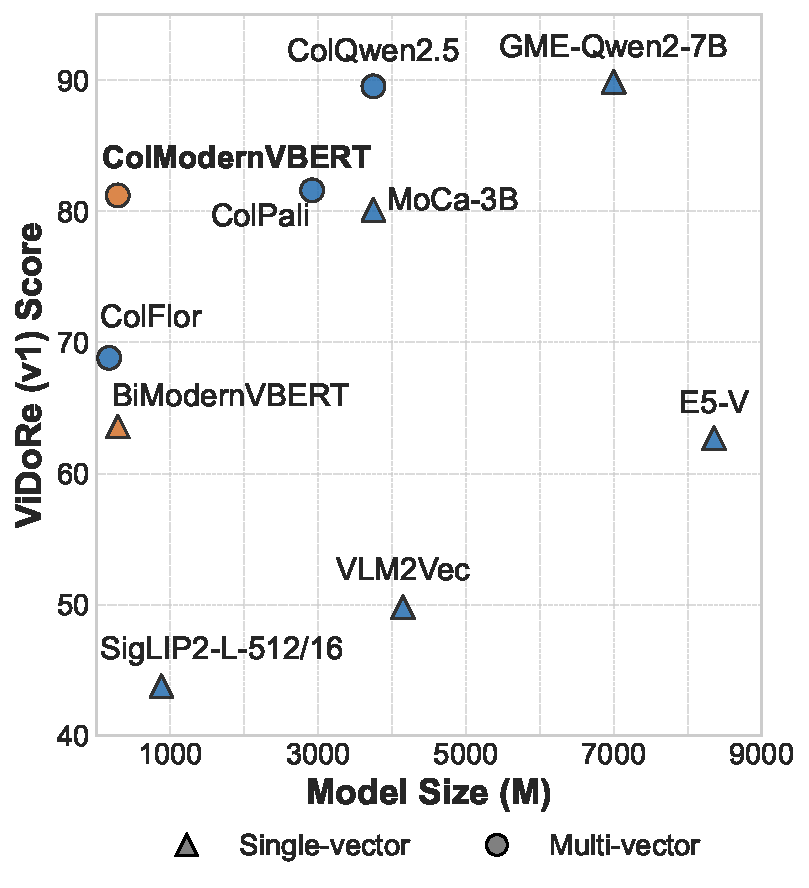
\includegraphics[width=\linewidth]{images/modernvbert_figures/fig_1/pareto_large_models_ColModernVBERT_orange.pdf}
%   \caption{\textbf{Pareto efficiency.} \colflagship{} outperforms models in its category on ViDoRe, achieving a leading performance-size tradeoff.
%   }
%   \label{fig:pareto_vidore}
%   %\vspace{-10pt}                         % tighten bottom spacing (tweak as needed)
% \end{wrapfigure}
This approach suffers from several limitations: OCR and layout parsing can be brittle and slow, complex visual elements such as tables, figures, and typography are often poorly captured, and any error or bias introduced during preprocessing is propagated to the retriever. % Recent work has shown that these multi-stage text pipelines can underutilize the rich visual structure of documents and leave significant performance on the table, especially in visually intensive domains \sidecite{faysse2025colpaliefficientdocumentretrieval}. 

\textit{Visual Document Retrieval} (VDR) has emerged as a compelling alternative to such text-based systems. Rather than indexing pre-extracted textual content, VDR models directly operate on page screenshots: given a user query, they retrieve relevant document pages by matching the query against image-based representations of the pages \sidecite{faysse2025colpaliefficientdocumentretrieval}. By bypassing OCR and layout parsing, VDR yields simpler end-to-end pipelines, significantly reduces indexing latency, and better exploits visual cues such as layout, figures, and fonts, while achieving strong performance on visually rich benchmarks like ViDoRe. 

\textbf{Limits of Generative VLM Repurposing.} Most current VDR systems are obtained by repurposing large generative vision–language decoders ~\sidecite{alayrac_flamingo_2022} as retrieval encoders via post-hoc contrastive fine-tuning \sidecite{ma2024unifyingmultimodalretrievaldocument, faysse2025colpaliefficientdocumentretrieval, jiang2024vlm2vectrainingvisionlanguagemodels}. While cost-efficient, this design choice bottlenecks retrieval performance and efficiency: model sizes, attention patterns, image resolutions, and training objectives are designed for generative use cases rather than optimized for retrieval which has been shown in text models to be suboptimal \sidecite{lee2024nvembedimprovedtechniquestraining, gisserotboukhlef2025pretrainencodersmaskedlanguage}. Furthermore, scaling trends \sidecite{wei2022emergentabilitieslargelanguage} are less pronounced for embedding models; while correlated with model size, strong retrieval performance remains attainable with small models \sidecite{clavié2024bettermonolingualjapaneseretrievers}.

% Learning rich embeddings aligned between text and image modalities remains a central challenge in visual retrieval.
% A core challenge in visual retrieval is learning text–image embeddings that faithfully encode complex, multi-level semantics—from fine-grained details to high-level concepts.
% For many years, \emph{contrastive pre-training} of dual encoders, typically pairing a vision transformer (ViT)~\sidecite{dosovitskiy_image_2020} with a text encoder, was the standard approach for generating cross-modal embeddings~\sidecite{radford_learning_2021, zhai_sigmoid_2023}. Owing to the performance improvements enabled by generative vision–language models (VLMs), recent work has increasingly explored repurposing these models as multimodal encoders through extended contrastive post-training~\sidecite{ma2024unifyingmultimodalretrievaldocument, faysse2025colpaliefficientdocumentretrieval, jiang2024vlm2vectrainingvisionlanguagemodels}. 






% While this approach capitalizes on the inherent capabilities of the backbone generative model to address complex visual tasks~\sidecite{alayrac_flamingo_2022}, it is unclear whether the design decisions made for generative purposes hinder the models when repurposed for representation learning. 
% Typically, generative VLMs are built as vision extensions to Large Language Models designed for autoregressive generation, often with a focus on strong knowledge and reasoning skills.

% Typically, VLM-based encoders inherit the causal attention masks VLMs are trained with, which has been repeatedly shown to be suboptimal for embedding tasks~\sidecite{li2023generaltextembeddingsmultistage, behnamghader_llm2vec_2024, lee2024nvembedimprovedtechniquestraining, springer2025repetitionimproveslanguagemodel, gisserotboukhlef2025pretrainencodersmaskedlanguage}. 



% Another notable architectural property of contemporary VLMs is their high parameter counts. LLMs exhibit emergent abilities in reasoning and knowledge use as they grow in size \sidecite{wei2022emergentabilitieslargelanguage}, and most openly released decoders and their vision-augmented variants are at least several billion parameters. Interestingly, scaling trends are less pronounced for embedding models: while size remains a performance factor, compact encoders often almost rival the performance of much larger ones, indicating diminishing returns with additional parameters \sidecite{muennighoff_mteb_2022}. 
% Visual retrieval benchmarks such as ViDoRe and MIEB ~\sidecite{xiao2025miebmassiveimageembedding} are no exception, and model sizes within a same model family has been shown to deliver clear, but limited gains. Taken together, this 

% This suggests it is likely possible to achieve strong visual representation quality with relatively small, well-trained models, especially leveraging late interaction methods \sidecite{clavié2024bettermonolingualjapaneseretrievers}.



% What are we doing?
% \manu{Important not to be redundant with contributions detailed later on. --> In this paper, we opt to build document retriever models from the ground up, freeing ourselves from the constraints of strating from repurposed VLMs. Our contributions are the following:}
% \noindent\textbf{Revisiting Design Decisions in VLM Decoder Embedder Models.} 
% \manu{would be nice to introduce a bit more about the fact we are conducting controlled ablations. somethikgn along the line of - principled ablatioons have been done for vision models, for text models but not for vlms which are recent. this paper fills the gap. One thing we could put some emphasis on is how we "selected" the modality alignement mix to particularly be interesting for document retrieval (whether this is true or false, we make it sound like that. another key point is modality transfer for contratsive which is a cool "princiupled"result }
Recent papers and model releases in the visual retrieval space have claimed performance improvements by scaling the amount of contrastive data and the compute budget \sidecite{zhang2025gmeimprovinguniversalmultimodal, xu2025llamanemoretrievercolembedtopperforming}, modifying the attention mask \sidecite{chen2025mocamodalityawarecontinualpretraining}, increasing image resolutions \sidecite{cohere_introducing_2024} or by introducing more diverse tasks and data sources \sidecite{jiang2024vlm2vectrainingvisionlanguagemodels}. %Furthermore, it remains unclear whether the performance gains offered by these models are due to improved image representation capabilies or rather are enabled by aligned text and visual latent spaces.

% In this work, we revisit the entire training pipeline for visual document retrieval through controlled experiments, identify key design factors for effective VDR (including attention masking, image resolution, modality alignment data regimes, and late-interaction–centric contrastive objectives), and introduce ModernVBERT, a compact 250M-parameter vision–language encoder that outperforms recent VDR models up to ten times larger on document retrieval tasks, while enabling efficient inference on cheap CPU hardware.


In this work, we attempt to centralize these efforts and systematically disentangle the impact of core design decisions in visual retriever training. 
% Through rigorous experimentation in controlled setups, starting from language model pretraining to multi-stage domain specific finetuning, we attempt to identify: \textit{What makes a visual retriever great?} 
% By systematically disentangle the impact of core design choices in visual retriever training. 
Through controlled experiments—ranging from language model pretraining to multi-stage, domain-specific fine-tuning, we aim to answer a central question:
% \anto{On ne fait pas vraiment de language model pretraining - non mais on conbtrole pour ca}

\begin{center}
\textit{Which design choices best boost performance in modern visual document retrievers?}
\end{center}

% In this work, we take a principled approach ourselves how to best train a visual encoder from the ground up - freeing ourselves from the constraints of starting from pretrained VLMs. Our contributions are the following:

% \noindent\textbf{Contribution 1.}\; We critically reassess the core assumptions in multimodal encoder design. Contrary to the prevailing view, \textit{our analyses show the main strength of VLM-based encoders is not better image embeddings, but stronger alignment between image and text token embeddings}. Through controlled experiments, we measure the role of alignment length, training duration, and cross-modality interactions. We show alignment effectiveness is task-dependent, and provide evidence that causal attention is suboptimal in visual document retrieval, especially with late interaction~\sidecite{khattab2020colbert, faysse2025colpaliefficientdocumentretrieval}. \manu{something about causal attention here would make sense maybe ?}

% \manu{Is this still a contribution ? do we want to back up these claims ? esp. if the claims are document leaning ?}
% \noindent\textbf{Contribution 2: \natcap{}.}\; Existing contrastive datasets consist mainly of web-collected image–caption pairs or image–label pairs. Yet these pairs are often either too general (generic captions) or too narrow (single labels), lacking the contextual richness available in backbone LMs. To address this, we introduce \natcap{}, a contextualized image–caption dataset. We synthetically generate captions from classification training sets by providing the model with the image, its label, and task metadata as context. Through dataset ablations, we show that \natcap{} can be particularly beneficial for zero-shot classification tasks.

% \noindent\textbf{Contribution 3: \flagship{}.}\; Building on these insights, we design and release \flagship{}, \paul{double check this} the first multimodal encoder that aligns a pretrained language model encoder with a CLIP vision tower through Masked Language Modeling (MLM) objective. \paul{check ce qui suit avec les resultats} Despite its modest size and low data regime \manu{why low data regime ? prefer something like modest training budget}, this encoder outperforms \manu{give scale} larger VLM-based models on document retrieval while remaining competitive on natural image benchmarks \manu{the competitive natiure of ilages is something we want to claim ?}. Our results demonstrate that strong, efficient vision encoders can be obtained without the excessive parameter counts and architectural limitations of repurposed generative VLMs.

%\noindent\textbf{Contribution 1.}\; We revisit core assumptions in visual retriever design, showing that token-level objectives—beyond coarse contrastive alignment—are main drivers of retrieval performance, and that beyond strong image features, overlooked gains lie in improved fine-grained image–text alignment. We further show that causal attention is suboptimal in document retrieval, with bidirectional masking offering clear improvements in multi-vector settings, and that other parameters such as image resolution data mixes should not be overlooked in the training pipeline.

\noindent\textbf{Contribution 1.}\; We revisit core assumptions in visual retriever design, showing that token-level training objectives benefit retrievers by strengthening image–text token alignment—rather than merely producing stronger image embeddings.
Our results indicate that causal attention is suboptimal in document retrieval, with bidirectional masking offering clear improvements in multi-vector settings, and that other parameters such as image resolution data mixes should not be overlooked in the training pipeline.

% \noindent\textbf{Contribution 1.}\; We revisit core assumptions in visual retriever design. 
% % Token-level objective improves visual document retrieval performance
% We observe that token-level objectives consistently enhance document retrieval performance, and that beyond the use of strong image features, early fusion models yield overlooked benefits through improved fine-grained image–text alignment.
% % Causal attention is suboptimal in visual document retrieval, bidirectional attention unlock full potential of late inetraction, and other parameters such as image resolution and data mixes should not be overlooked.
% We further show that causal attention is suboptimal in visual document retrieval, with bidirectional masking offering clear improvements, and that other parameters such as image resolution data mixes should not be overlooked in the training pipeline.

% \noindent\textbf{Contribution 1.}\; We revisit core assumptions in visual retriever design. Notably, we show that causal attention is suboptimal in multi-vector document retrieval, with bidirectional masking offering clear improvements as a counterpart. We further show that token-level objectives—beyond coarse contrastive alignment—are important drivers of retrieval performance, and that beyond strong image features, overlooked gains lie in improved fine-grained image–text alignment.

%We critically reassess the core assumptions in visual retriever design. 

%We show that token-level objectives are beneficial in document retrievers training, and that contrary to the prevailing view, the main strength of VLM-based encoders is not better image embeddings, but stronger alignment between image and text token embeddings due to this token-level training objective. 

%We provide evidence that \textit{causal attention is suboptimal for visual retrieval tasks, especially in multi-vector settings}. Like in generative tasks, we observe that visual document retrieval is resolution-sensitive, 

%and that a cooldown on high-resolution images during modality alignment can improve model performances in such tasks.

\noindent\textbf{Contribution 2: \flagship{}.}\; Building on these insights, we release \flagship{}, a small \flagshipparameters{} multimodal encoder that aligns a pretrained language encoder with a vision encoder through Masked Language Modeling (MLM) objective, and \colflagship{} a variant fine-tuned for document retrieval. Despite its modest size and limited training budget, \colflagship{} matches models 10x larger on standard visual document retrieval benchmarks, demonstrating the interest of designing a retrieval focused model from the ground up. 
% We publicly release the model, intermediate checkpoints, and the training code at \repo{}.
We release the model, intermediate checkpoints, and the training code at \repo.

% Our results demonstrate that performant vision retrievers can be obtained without the excessive parameter counts and architectural limitations of repurposed generative VLMs.

% \begin{figure}[ht]
%     \centering
%     \includegraphics[width=0.6\textwidth]{example-image.png}
%     \caption{\paul{TODO} \manu{This could also be a table about what the different ablations taught us (green checkmarks, red crosses. Pareto might be too childish}}
%     \label{fig:pareto_frontier}
% \end{figure}

% \begin{figure}[t]
%     \centering
%     \includegraphics[width=\linewidth]{images/modernvbert_figures/fig 1/vbert_visu_fig1.pdf}
%     \label{fig:schema_causal_bidir}
%     \caption{\paul{TODO}}
% \end{figure}

% \begin{figure}[t]
%     \centering
%     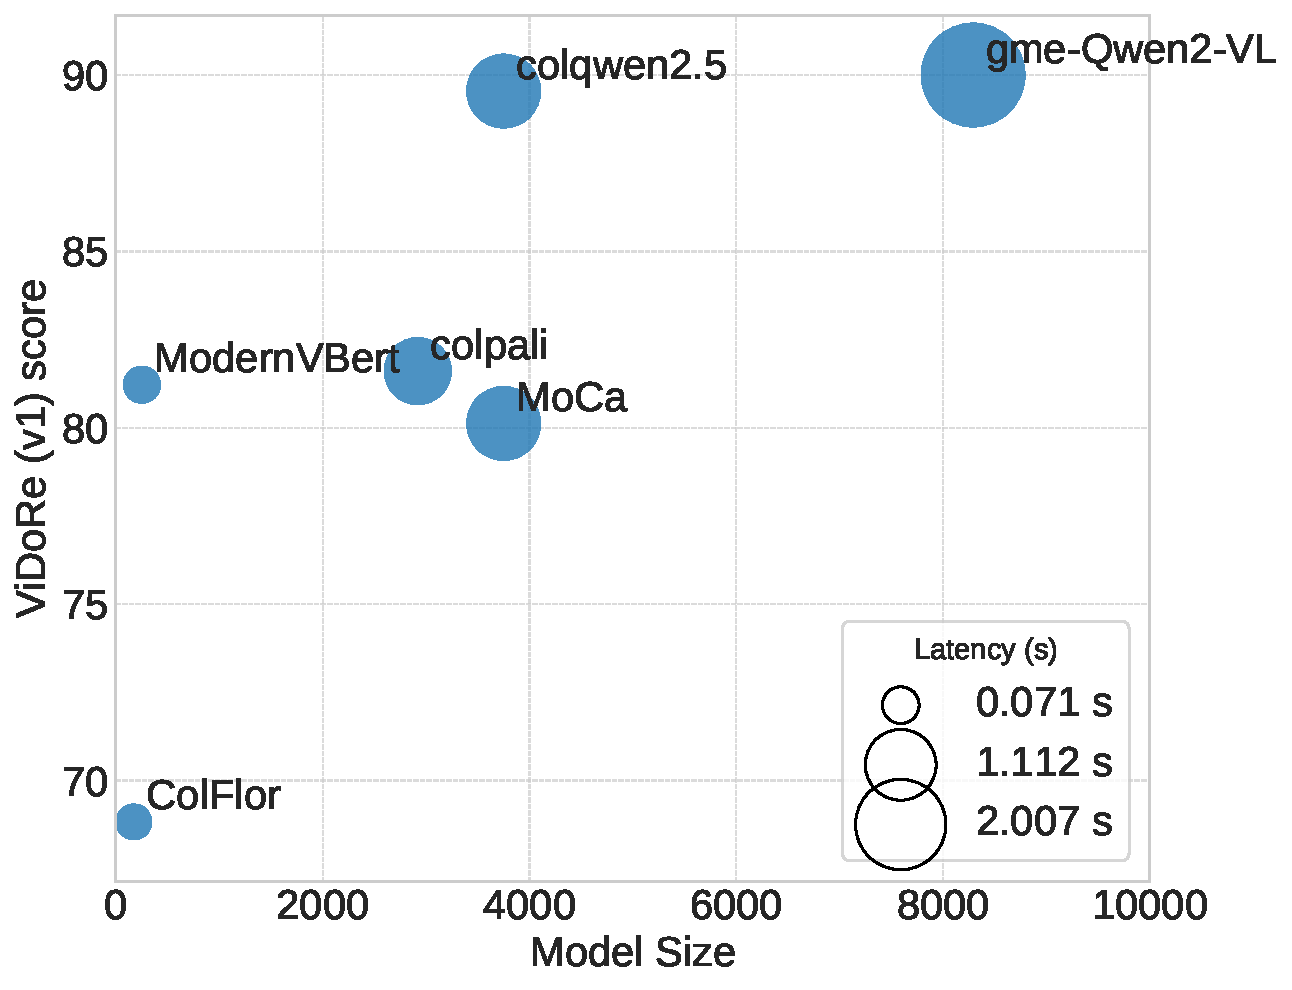
\includegraphics[width=0.5\linewidth]{images/modernvbert_figures/pareto_plot.pdf}
%     \label{fig:pareto}
%     \caption{\paul{TODO}}
% \end{figure}


% We show The primary advantage of modality alignment methods (MLM/CLM objectives) lies not in improved intrinsic image embeddings, but rather in their ability to project text and image tokens into a shared latent space. 
% On top of that many MODELS ARE CONTRASTIVELY UNDERTRAINED. IN FACT, IN MANY OFF THE SHELF MODELS, THE TRAINING WORSENS THE EMBEDDING CAPABILITIES WRT SIGLIP.  We argue the interest of VLMs as encoders mainly lie on tasks where complex alignment with natural language queries are key (document retrieval), and analyze the impact of scaling both the modality alignement and the contrastive training phase, showcasing much performance is still up for grabs by scaling the contrastive training. 

% IDENTIFY THE AREAS WHERE THEY OUTPERFORM SIGLIPS.

% \noindent\textbf{Contribution 2.}\; We revisit the debate between encoder-only and decoder-based architectures, providing empirical evidence that bidirectional encoders outperform causal decoders in embedding quality. Additionally, we show that the performance gap between decoders and encoders can be bridged through post-training decoders using masked language modeling (MLM) objectives, but emphasize that substantial training duration is necessary. This gap is particularly pronounced in late-interaction retrieval methods, which currently dominate document retrieval benchmarks, highlighting the critical role of bidirectional attention mechanisms.

% \smallskip
% \noindent\textbf{Generative VLMs as embedding models.}\;Recently, \emph{generative} vision–language models (VLMs) combine a pretrained image encoder together with a large autoregressive decoder to perform a wide variety of generative multimodal tasks.
% Researchers have begun to repurpose these VLMs by extracting the text model's hidden state, running contrastive pretraining, reporting state‑of‑the‑art (SOTA) numbers on emerging benchmarks, e.g.\ DSE, VLM2Vec on \textsc{MMEB}  and ViDoRe. To further boost retrieval performance in complex image retrieval (documents), ColPali has shown that the vision-text alignement at a token level that VLMs exhibit enable retrieval with a late interaction operation which match text query tokens to corresponding image patch tokens. 

% \smallskip
% \noindent\textbf{Do VLM decoders really improve the \emph{image} representation?}\;
% % Mention MIEB where best models remain contrastive
% Although these repurposed VLM embedding models showcase strong retrieval performance, especially on document retrieval and on tasks contained within their contrastive training sets, more comprehensive image embedding benchmarks such as MIEB tell a slightly different story. Across most natural image tasks, the best models remain dual encoders, and this is particularly true in settings without corresponding text vectors (typically image classification with fixed classes, clustering). In this work we question whether as commonly believed feeding image embeddings to a text models really enriches the image representation, or whether the text model just facilitates learning mappings between text and image parameters.  We also question the common design choices of leveraging a causal decoder for representation tasks, while for text embeddigns, bidirectional encoders have times and times agin shown to be superior. Building upon these insights, we make the following contributions:

% \noindent\textbf{Contribution 1.}
% % revisit the design choices behind VLM encoders
% % show constrastively trained models remain best for image represenations, and that MLM/CLM alignement mainly help project text and image tokens to a simimlar latent space 
% % argue that it is more importznt to scake contrastive training than anlignement or model size

% \noindent\textbf{Contribution 2.} %revisit encoder vs decoder debate and show bidirectoonal attention is best. Show that the gap can be bridged by post-training decoders with MLM but it needs to be long enough. Show the gap is particularly meaningful for late interaction models which are currently the top performaing models on document retrieval benchmarks.


% \noindent\textbf{Contribution 3.} 
% % Apply lessons and release a small yet strong vision encoder model specialized for document retrieval tasks in public, outperforming bigger models


% Collectively, our results suggest that future progress in multimodal retrieval should prioritize better interaction strategies and training objectives over merely scaling decoders, and that strong, efficient vision encoders remain within reach without sacrificing simplicity.



% \section{Introduction}
% % Intro on image representations / document retrieva using images

% \noindent\textbf{Using VLMs for representation learning.}
% % mention colpali, Document screenshot embedding (DSE, Ma 2024), vlm2vec

% \noindent\textbf{Gap.} 
% % While VLMs claim strong performance on MMEBN, Vidore whoch are retrieval benchjmaerk, heavy on complex text inputs, more extensive evaluations on MIEN show they underperform on most natural language tasks. Decoder vs encoder debate (cite work)


% \noindent\textbf{Contributions.}

\section{Methodology}\label{sec:methodology}

% \manu{remember our contribution. might be nice to have an intro paragraph that details our process. Here our goal is a rigorous study of various parameters during training. To do so, we place ourselves in a controlled envrionment where we wan modify N settings. Our base model is xxxx.}

% Our goal is to discuss core choices in the visual retriever training process. To do so, we place ourselves in a controlled environment that allows us to ablate parameters of this training. 

Our analysis aims at quantifying the impact of design decisions made when training visual retrievers. In opposition to previous work, we begin our analysis as early as language model modality alignment and iteratively study design choices by modifying design choices independently to reduce confounding factors as much as possible \sidecite{allenzhu2025physicslanguagemodels1}.


\noindent\textbf{Controlled Experimental Setup.}
A central point of interest is the impact of causal and bidirectional attention masks. While recently studied for textual representation applications \sidecite{gisserotboukhlef2025pretrainencodersmaskedlanguage, weller2025seqvsseqopen}, we extend the experiment to the vision modality. We use checkpoints released by \sidecite{gisserotboukhlef2025pretrainencodersmaskedlanguage} which consist in a series of identical 210M parameter transformer models based on the Llama architecture \sidecite{touvron_llama_2023} trained on 100B tokens that differ only in their attention masking strategy during language model training but that are perfectly identical in terms of training data seen, model size and architecture, learning rate scheduling, etc... The checkpoints we use are \texttt{enc} a bidirectional encoder trained with Masked Language Modeling (MLM), \texttt{dec}, a causal decoder trained with next token prediction, and \texttt{dec-enc} a causal decoder annealed over the end of its textual training by removing the causal mask and switching the training objective to MLM. For the vision tower, we employ the vision component of \texttt{siglip2-base-16b-512} \sidecite{tschannen2025siglip2multilingualvisionlanguage}, a 86M parameter vision transformer contrastively trained on billions of text-image pairs.
All ablations thus stem from iso-data controlled setups, and as further described, are further trained on the same data sequence, with the same batch sizes, optimizers, schedulers and on the same hardware.
% For this purpose, we leverage the checkpoints released by , which provide this rigorously controlled setting. In addition, we include a decoder model from this work that was annealed with MLM objectives, allowing us to evaluate whether decoders can effectively transition into encoders prior to modalities alignment~\sidecite{gisserotboukhlef2025pretrainencodersmaskedlanguage, weller2025seqvsseqopen}. 
%We use SigLIP2-16B-512 as vision encoder.
% \paul{ablation runs table?}
%The full set of ablation model configurations is summarized in Appendix~\ref{appendix:ablation_models}.

\begin{figure}[t]
    \centering
    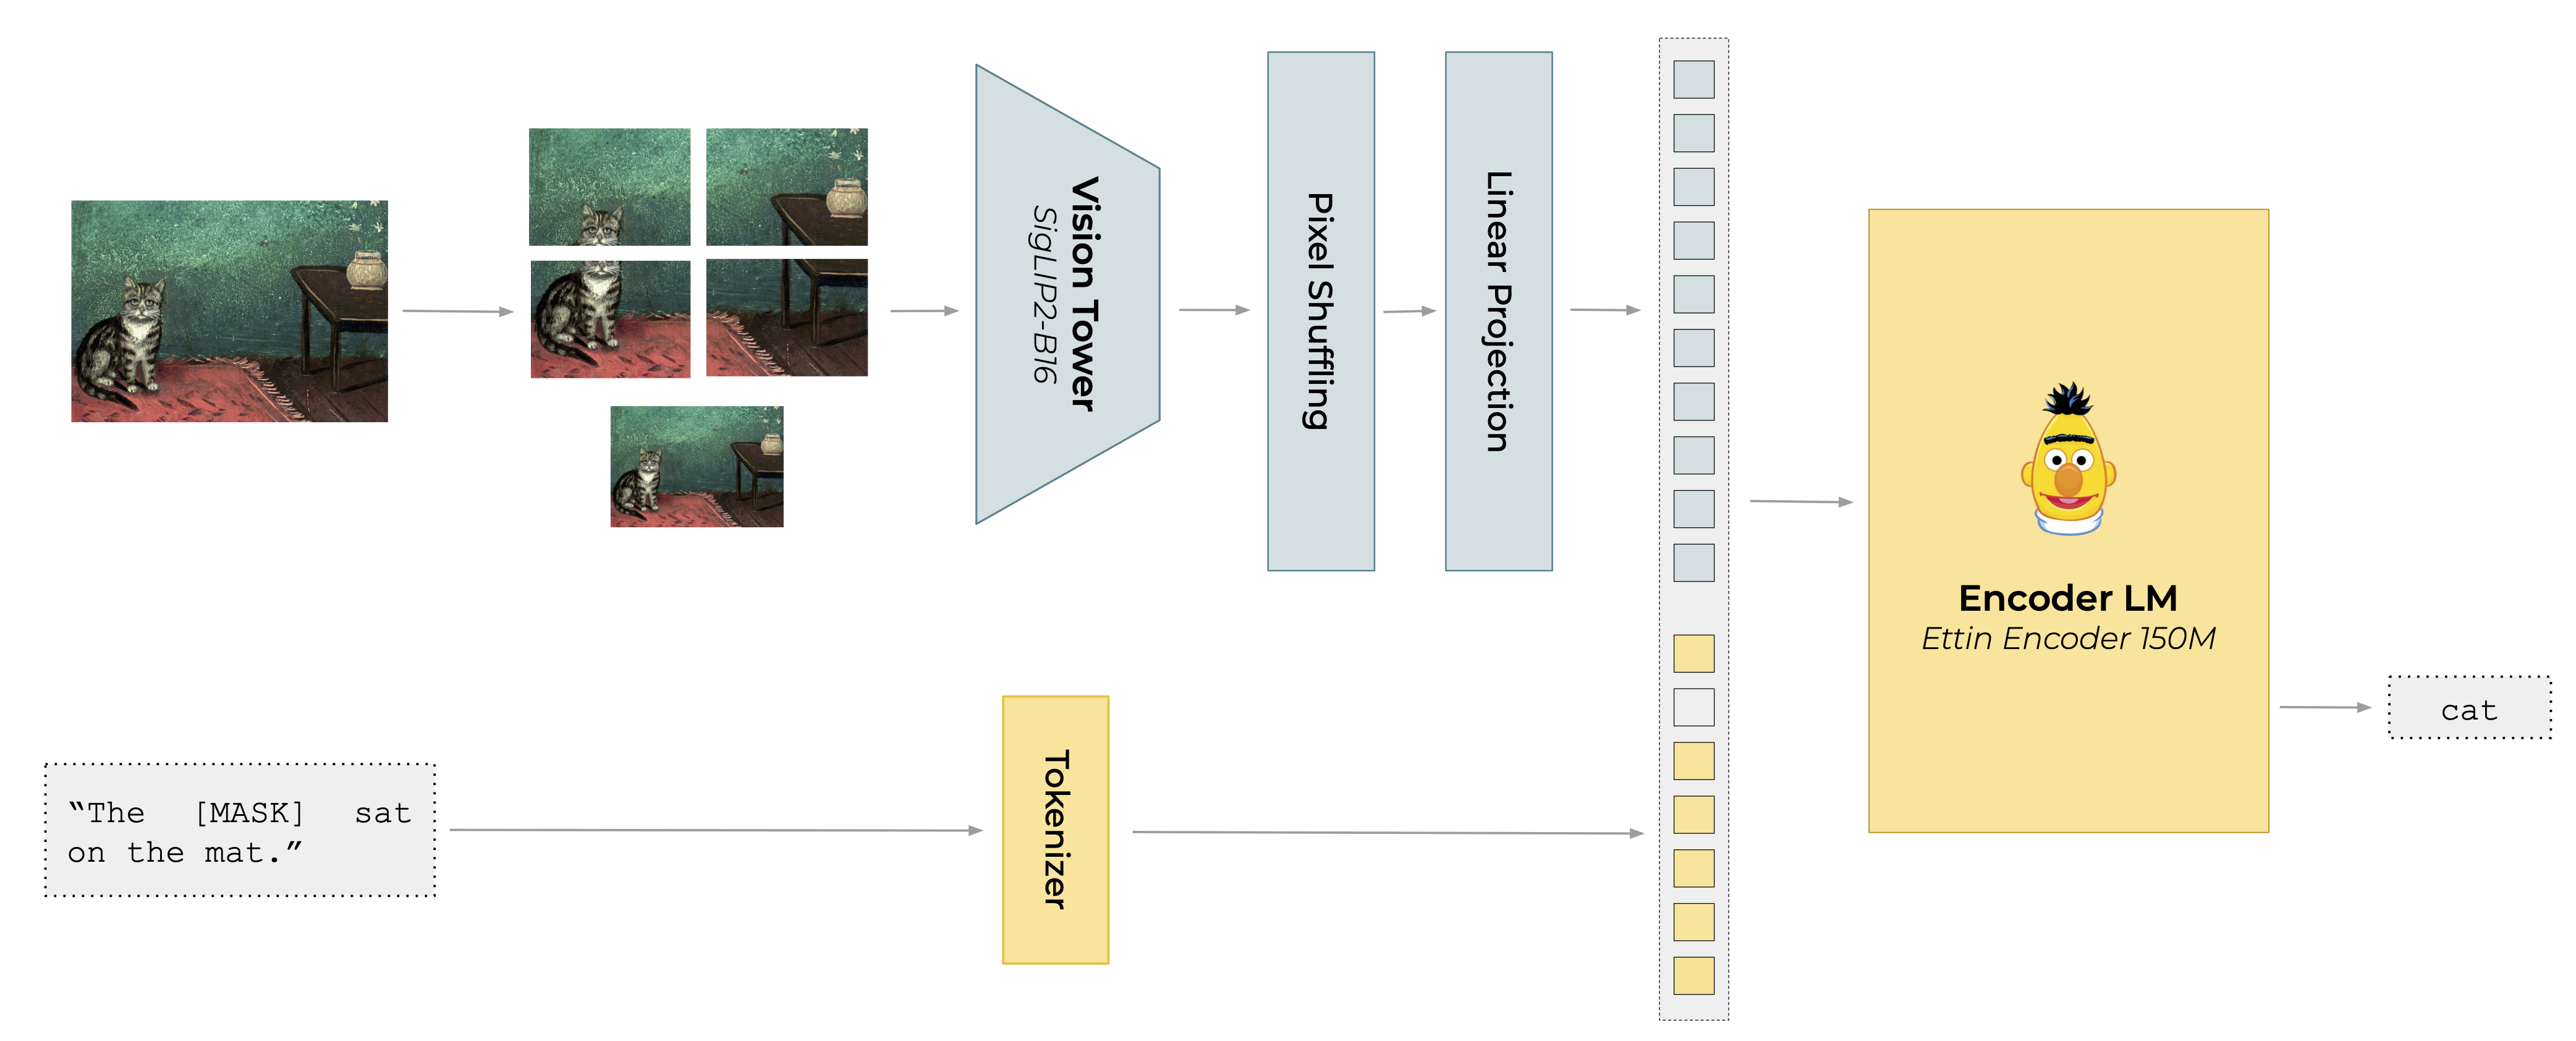
\includegraphics[width=0.99\textwidth]{images/modernvbert_figures/vbert_architecture.png}
    \caption[Early fusion architecture]{
    \textbf{MLM-based early fusion architecture.} The visual encoder produces patch representations, which are passed to a language model. 
    %We apply pixel shuffling to compress the visual representations produced by the vision tower.
    Our end-to-end bidirectional attention fused architecture is trained with Masked Language Modeling objectives and is perfectly suited for sequence and token-level representation tasks.}
    \label{fig:lf_architecture}
\end{figure}

\noindent\textbf{Model Architecture.}  
Our analysis are not centered around model architectures and to draw broadly applicable insights, we design vision-language models following current standard training practices.  In line with most recent work, we employ the early fusion architecture \sidecite{alayrac_flamingo_2022} illustrated in Figure~\ref{fig:lf_architecture}, in which visual patch embeddings produced by the vision encoder are projected into the language model input embedding space and concatenated with text token embeddings to encourage joint processing ~\sidecite{li2022blipbootstrappinglanguageimagepretraining, alayrac_flamingo_2022, wang2024qwen2vlenhancingvisionlanguagemodels, yang2025qwen251mtechnicalreport, marafioti2025smolvlmredefiningsmallefficient}. As described in \autoref{sec:modality-align}, we generalize the training loss to function both with causal and masked language modeling objectives.  
To handle dynamic resolutions, we split large images into 512$\times$512 pixel tiles as expected by the SigLIP encoder\sidenote{Images are downscaled (or upscaled) so that the lengths and widths reach a multiple of 512 pixels to preserve the aspect ratio, padding is used on the smaller side when necessary (i.e. a 1024x1000 px image would be padded to 1024x1024 px).}. Following current standard practices, we further process a downscaled version of the full image to improve inter-tile consistency and global visual understanding~\sidecite{lin2023sphinxjointmixingweights, ye2023ureaderuniversalocrfreevisuallysituated}. The vision tower produces 1024 pixel patch representations for each tile\sidenote{The SigLIP tower takes 512x512 px images and process them by 16x16 px patches \cite{dosovitskiy_image_2020}. This results in $(512/16)^2=1024$ patches.}, which we  compress to 64 tokens through \textit{pixel shuffling}~\sidecite{shi2016realtimesingleimagevideo} with a compression ratio $r=4$, following prior work on models of comparable size~\sidecite{marafioti2025smolvlmredefiningsmallefficient}. We highlight the impact of image resolution and this parameter on the number of visual tokens in Appendix~\ref{appendix:visual_tokens}.

% To handle dynamic resolutions, we split large images into 512$\times$512 pixel patches as expected by the SigLIP encoder, and further concatenate a downscaled version of the full image to improve inter-patch consistency and global visual understanding following current standard practices ~\sidecite{lin2023sphinxjointmixingweights, ye2023ureaderuniversalocrfreevisuallysituated}. To compress the information from sequences of large images, we apply pixel shuffling~\sidecite{shi2016realtimesingleimagevideo} with a ratio of $r=4$, following prior work on models of comparable size~\sidecite{marafioti2025smolvlmredefiningsmallefficient}.

% Note that we do not employ vision encoders with native resolution and RoPE-2D, as our focus is solely on single image representation learning using compact models. In this context, the additional computational overhead of such encoders is not justified.\paul{draft, I have to read qwen2vl carefully and understand the tradeoff more clearly}



% \noindent\textbf{Controlled Experimental Setup.}  
% We build on the publicly available checkpoints of \sidecite{gisserotboukhlef2025pretrainencodersmaskedlanguage}, which provide a fully controlled environment: all models share identical architectures, parameter counts, training datasets, and schedules, and differ only in the use of causal versus bidirectional attention masks. In addition, we include a decoder model from this work that has been annealed with MLM objectives, allowing us to evaluate whether decoders can effectively transition into encoder-like behavior. The full set of ablation models configurations is summarized in Table~\ref{tab:ablation_models}.

\noindent\textbf{Training Procedure.} Our experiments focus on retrieval performance. We employ a standard biphasic training procedure, in which we first run modality alignment to train a pretrained textual language model to understand visual inputs through language modeling objectives  ~\sidecite{liu_visual_2023} (\autoref{sec:modality-align}), then rely on a second text-image contrastive learning phase to learn efficient image representations ~\sidecite{radford_learning_2021} (\autoref{sec:contrastive_posttraining}). We further describe the general setup, and detail specific modifications to the default training procedure in the experiment section.

\subsection{Modality Alignment}
\label{sec:modality-align}
We align the vision encoder tower with the language model by training the image embedding projection layer to map visual features into the language model embedding space. The pretrained language model is also fine-tuned with Low-Rank Adapters (LoRA) \sidecite{hu_lora_2021}, allowing both image and text models to adapt jointly while reducing the risk of monomodal performance collapse \sidecite{alayrac_flamingo_2022, liu_visual_2023, laurencon_what_2024, mckinzie_mm1_2024, marafioti2025smolvlmredefiningsmallefficient}.

\noindent\textbf{Alignment Loss.} 
For decoder‑based models, we train with Causal Language Modeling (CLM) loss on the text tokens, as standardly done in VLM modality alignment:
\begin{equation}
\mathcal{L}_{\text{CLM}}
  = -\sum_{t=1}^{T} \log P_{\theta}\!\bigl(x_t \mid x_{<t}\bigr),
\end{equation}

where $x_{<t}$ denotes all tokens preceding position $t$. We generalize this training scheme to bidirectional encoders models, by using the Masked Language Modeling (MLM) loss on the textual tokens:
\begin{equation}
\mathcal{L}_{\text{MLM}}
  = -\sum_{t \in \mathcal{M}} \log P_{\theta}\!\bigl(x_t \mid x_{\backslash\mathcal{M}}\bigr),
\end{equation}
where $\mathcal{M}$ is the set of masked token positions and
$x_{\backslash\mathcal{M}}$ is the input with those tokens masked out.


\noindent\textbf{Modality Alignment Corpus.} Models are modality aligned on a large corpus in large parts derived from The Cauldron 2~\sidecite{laurencon_what_2024} and Docmatix~\sidecite{laurençon2024building}. Our objective being to train document focused retrieval models, we use an adjusted training mixture that upsamples images containing text and documents with varying level of complexities. Our final training corpus consists of approximately 2B text tokens, and includes diverse sources such as web pages, books, and scientific papers. Mixture details are given in Appendix~\ref{appendix:alignment_mixture}. We note that controlling the exact data distribution during this phase enables the models we train to specialize early and achieve good document focused downstream performances which many large models struggle with \sidecite{liu_improved_2023}.

\noindent\textbf{Parameters.} All models are trained using a masking ratio of 0.5 and user-prompt masking to avoid overfitting on chat-template format~\sidecite{huertaenochian2024instructionfinetuningdoesprompt, shi2024instructiontuninglossinstructions, allal2025smollm2smolgoesbig}. We employ WSD scheduler~\sidecite{hu2024minicpmunveilingpotentialsmall} with the first 5\% of the training as warmup, the last 20\% as decay and a maximum learning rate of 1e-4. The ablation models are aligned on 3.5B tokens. We provide additional details on the training setup in Appendix~\ref{appendix:implementation_details}.

\subsection{Contrastive Post-Training}
\label{sec:contrastive_posttraining}
Once the language model has learned to process image tokens jointly with text tokens, we specialize models through a contrastive post-training stage designed to enhance the semantic representation of the output embeddings produced by the model \sidecite{reimers2019sbert}. 

% We use a contrastive learning objective to modify the latent space of our base model to adapt it for similarity tasks. 

%We generate embeddings by mean pooling \maxou{cite paper backing this choice} token embeddings for encoder-based models, and by selecting the EOS token embeddings for decoder-based models \maxou{potentially here too? e.g. Qwen3-Embeddings}. 

\noindent\textbf{Post-training Pairs.} The post-training dataset used as starting point in our ablations comprises 118k document-query pairs from the ColPali corpus~\cite{faysse2025colpaliefficientdocumentretrieval} as well as another 118k of natural image-description pairs from the MSCOCO train set~\sidecite{lin_microsoft_2014}.

\textbf{Contrastive Loss.} We employ the InfoNCE loss~\sidecite{oord_representation_2018}, defined as

\begin{equation}
\mathcal{L}_{\text{InfoNCE}}(\mathbf{q},\mathbf{d^+})
  =-\log\frac{\Phi(\mathbf{q},\mathbf{d^+})}{\Phi(\mathbf{q},\mathbf{d^+}) + \sum_{\mathbf{d^-}\in\mathcal{N}_q}\Phi(\mathbf{q},\mathbf{d^-})},
\end{equation}

where $\mathbf{d^+}$ denotes the positive target for the query $\mathbf{q}$, $\mathcal{N}_\mathbf{q}=\mathcal{N}_\mathbf{q}^{\text{in}} \cup \mathcal{N}_\mathbf{q}^{\text{hard}}$ the set of negative targets (in-batch and hard negatives when mentioned), and $\Phi(\mathbf{q},\mathbf{d})$ a similarity function between the token(s) of the query and the documents.\sidenote{We use the last (EOS) token for causal models, and mean pool all sequence tokens for bidirectional encoders for single-vector models. Alternatively, we use all document and query tokens without pooling for late interaction matching \cite{faysse2025colpaliefficientdocumentretrieval}. Details in Appendix~\ref{appendix:similarity_functions}}. 
For general-domain post-training we compute the loss symmetrically~\sidecite{radford_learning_2021}.

\textbf{Batches Curation.} In contrastive learning, batch diversity critically impacts retrieval entropy. Overly heterogeneous batches lead to trivial retrievals, while curated batches yield richer training signals. We employ task-aware batching~\sidecite{li2023generaltextembeddingsmultistage}, grouping documents by source to ensure a homogeneous batch composition.


\subsection{Ablation Evaluation Setup}


The contrastively trained models are evaluated on retrieval and zero-shot classification tasks across multiple domains. Although the main focus remains document retrieval capabilities, evaluated by aggregating scores from the ViDoRe and ViDoRe v2\sidenote{\label{fn:vidorev2}We report only the English splits of ViDoRe v2, as our base models are trained on English data only.} \sidecite{macé2025vidorebenchmarkv2raising} benchmarks (nDCG@5), we also assess more generalist image retrieval capabilities by selecting tasks from MIEB~\sidecite{xiao2025miebmassiveimageembedding}. For natural image retrieval, we aggregate MSCOCO retrieval ~\sidecite{lin_microsoft_2014} and Flickr30k retrieval (nDCG@10) \sidecite{plummer_flickr30k_2015} test sets. Finally, following practices in \sidecite{muennighoff_mteb_2022}, we assess both zero-shot and fine-tuning abilities of our models on general classification tasks. Specifically, we measure classification accuracy by fine-tuning a logistic regression head on top of our model's embedding on Stanford Cars~\sidecite{6755945} and Food101~\sidecite{10.1007/978-3-319-10599-4_29}, and we evaluate zero-shot performance on FER2013~\sidecite{khaireddin2021facialemotionrecognitionstate} and EuroSAT~\sidecite{helber2019eurosatnoveldatasetdeep} and aggregate the results.


\section{What Makes a Great Visual Retriever?}

\begin{figure}[t] % <- 12 = approx. number of text lines to wrap
  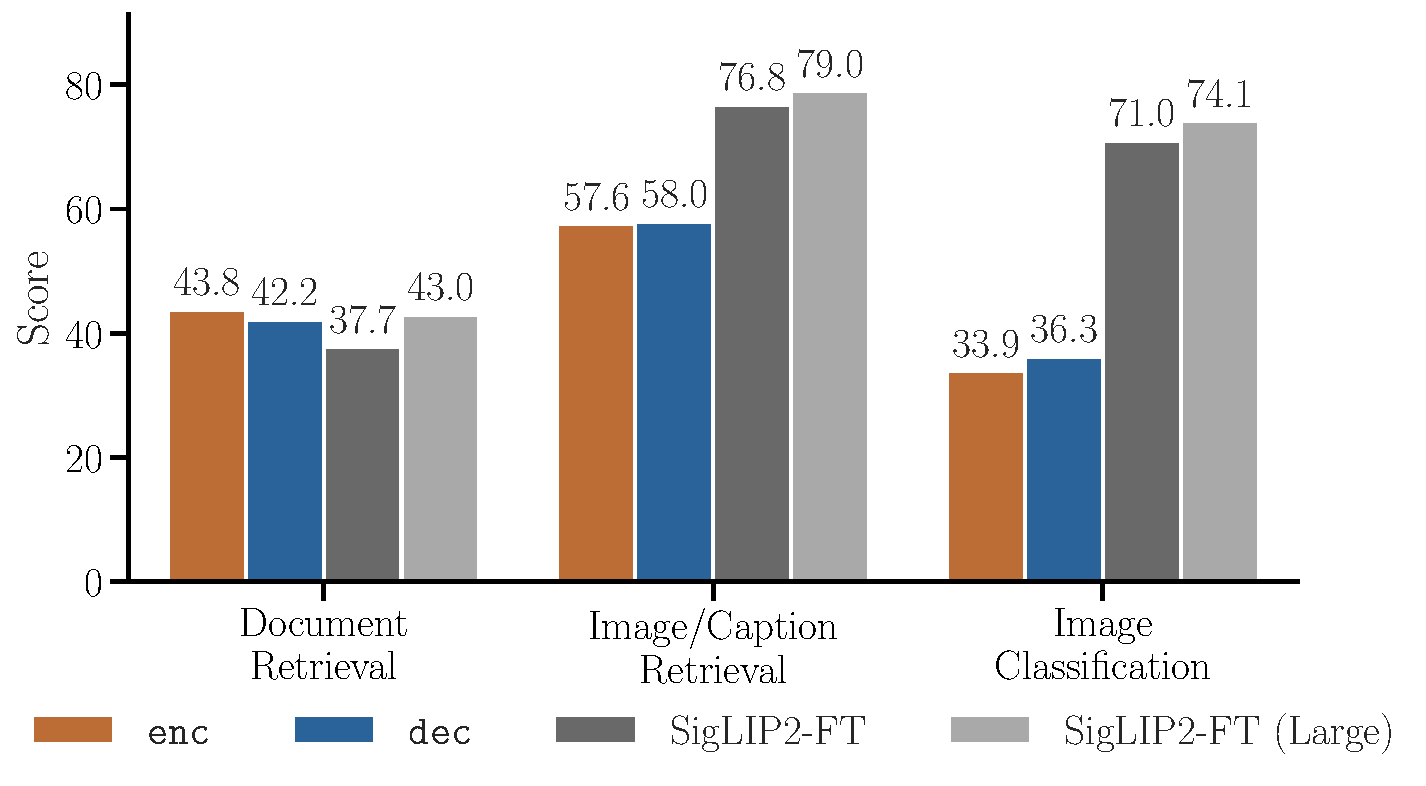
\includegraphics[width=0.95\linewidth]{images/modernvbert_figures/vbert_style/objective_downstream__rebuttal_ft.pdf}
    \caption[Modality alignment impact]{\textbf{Impact of Modality Alignment objective on downstream tasks.} Early Fusion of vision and text models boosts document retrieval tasks regardless of the LM objective, but degrades natural image and classification tasks w.r.t. the standalone \textit{fine-tuned} vision model SigLIP. Reported scores are aggregated MIEB scores (nDCG, Accuracy.)}
    \label{fig:objective_downstream}
\end{figure}


Vision-language retrievers built upon existing generative VLMs often inherit design choices and weights that may not be well suited for all embedding tasks. Here, we analyze these critical design choices hoping to derive clear insights for developing efficient visual retrievers. Importantly, although we assess design decisions at different stages of the training pipelines, evaluation are always done end-to-end on the final evaluation signal. 

%\anto{Suggestion for intro paragraph: Many vision-language retrieval systems adapt pre-trained generative models, but their weights are often not optimized for creating effective embeddings. In this section, we analyze the critical design choices in this adaptation process to provide clear guidelines for developing more efficient retrievers.}

\subsection{Modality Alignment Design}
\label{sec:ablation_tasks}

\noindent\textbf{Language modeling Modality Alignment improves document understanding.}
% According to benchmarks such as MIEB~\sidecite{xiao2025miebmassiveimageembedding}, dual encoder models trained explicitly on contrastive image-text tasks achieve superior performance in image classification tasks compared to VLMs. VLMs particularly excel at retrieving complex text-image relationships~\sidecite{jiang2024vlm2vectrainingvisionlanguagemodels}, yet, contrary to common belief, they do not enhance image representations themselves. In fact, they degrade performance in most natural image benchmarks. Instead, their strength lies in effectively aligning text and image tokens for zero-shot classification\paul{find work}. To substantiate this hypothesis, we designed experiments on document classification tasks, pooling image representations and applying classification heads. Results demonstrated that standalone image encoders possess sufficient capacity and information for these tasks, ultimately converging to similar performance levels regardless of the VLM training. This confirms that the critical contribution of VLMs lies in the modality alignment phase. For natural images, token-level alignment appears less critical, and the high-level features learned through large-scale contrastive training, as exemplified by SigLIP, are more impactful. Thus, contrastive training aligned with retrieval scenarios at inference is essential. \paul{What should we present here? Would results from @QM xp fit? Maybe we should focus on classification tasks here and stop reporting it later}
% On the other hand, these latest particularly excel at retrieving complex text-image relationships like documents-query ones~\sidecite{jiang2024vlm2vectrainingvisionlanguagemodels, chen2025mocamodalityawarecontinualpretraining}.
According to benchmarks such as MIEB~\sidecite{xiao2025miebmassiveimageembedding}, dual encoder models explicitly trained on contrastive image-text tasks outperform repurposed VLMs in natural image classification tasks. 
% We first study the impacts of aligning a pretrained Language Model (LM) with a vision tower through language modeling objectives, across different tasks.
%Using the checkpoints described in \autoref{sec:methodology}, 
To assess this, we train an encoder and a decoder vision-language model using the methodology described in \autoref{sec:methodology} on a mix of natural image and document data (alignment and contrastive training). We compare them with \textit{SigLIP2-FT}, the 378M dual vision encoder model whose vision component is used by the vision tower of both VLMs, and with the larger \textit{SigLIP2-FT Large} (881M parameters). Both SigLIP-FT models are finetuned in the same conditions as the VLMs, and initialized from pre-trained weights from scratch on billions of text-image pairs\sidenote{We report the performance of the untrained \textit{off-the-shelf} SigLIP in Appendix~\ref{appendix:objective_downstream}}.
As shown in Figure~\ref{fig:objective_downstream}, the two early fusion VLM variants severely underperform the SigLIP2-FT dual encoders on natural image tasks. In contrast, they achieve significant gains on document retrieval tasks (+6.1 nDCG@5 on ViDoRe and ViDoRe v2 datasets w.r.t. base), even edging out \textit{SigLIP2-FT Large} that contains 3.5x vision parameters more than both VLMs.

% This confirms high-level representation tasks do not benefit from the granular interactions between image and text tokens learned during the VLM modality alignment phase, but large-scale contrastive training remains superior. However, pairing a vision model with an LM enables token level interactions that create richer document understanding, aiding specific tasks even with less contrastive post-training.

This confirms large-scale contrastive training remains best for high-level image representation tasks (natural images), but sequentially combining a vision model with a pretrained language model facilitates document representation tasks, even with significantly less contrastive post-training. As the rest of this paper shows, steering away from the dual encoder architecture further enables improving performance through many avenues other than text to image contrastive training, for which supervised training samples can be hard to obtain.


% \begin{figure}
%     \centering
%     \includegraphics[width=0.9\linewidth]{images/modernvbert_figures/objective_downstream.png}
%     \caption{Impact of different objectives on downstream tasks. Aligning a language model with a vision tower through language modeling pretraining improves the performance of the model in document retrieval tasks. However, it degrades its performances in caption retrieval and classification tasks.}
%     \label{fig:objective_downstream}
% \end{figure}

% \noindent\textbf{Scaling the pretraining phase for better token representations.}  
% Prior work shows that scaling the pretraining phase of causal VLMs improves their generative abilities~\sidecite{beyer2024paligemmaversatile3bvlm, mckinzie_mm1_2024, wang2024qwen2vlenhancingvisionlanguagemodels}. We test whether similar gains hold in a bidirectional setting by evaluating checkpoints during pretraining with an MLM objective, up to 3.5B tokens. We compare this approach with the traditional CLM objective. Figure~\ref{fig:pt_scaling} presents the performance of the two training objectives across a diverse set of tasks. 
% The model improves across all tasks with additional pretraining data, showing the importance of scaling this phase. \textit{CLM offers an advantage in low-data regimes, but MLM seems to catches up and scales more effectively}. In document retrieval, MLM surpasses CLM.  
% % MLM scale better than CLM, especially in documental settings  
% % To counterbalance this plateau, we anneal the CLM-aligned decoder model using MLM to bring this objective scaling benefits. However, we observe a negative impact of such attention adaptation during cooldown. This might come from our model and scale, which may be too low to observe these gains.  
% % CLIP is the king in natural images  
% Image captioning and classification performances drop compared to the CLIP baseline vision tower. In contrast, the vision tower baseline is quickly outperformed in document retrieval. This finding suggests that \textit{token prediction pretraining yields embeddings better suited for document tasks than fully contrastively trained models}.  


% \begin{figure}[t]
%     \centering
%     \includegraphics[width=0.9\linewidth]{images/modernvbert_figures/pt_scaling.png}
%     \caption{Pretraining phase scaling. The dashed line marks the vision tower baseline. The orange curve shows the model initialized from a decoder LM with a \textit{CLM} objective, and the blue curve shows the model trained with an \textit{MLM} objective from an encoder LM. CLM performs better in low-data regimes, but MLM scales more effectively, surpassing CLM in document retrieval, while captioning and classification remain below the CLIP baseline.}
%     \label{fig:pt_scaling}
% \end{figure}


% \textit{Given that the initial training stage aims to align representations at the token level~\sidecite{jiang2024vlm2vectrainingvisionlanguagemodels}, we next evaluate whether MLM constitutes a more effective objective for learning multi-vector representations.}


\noindent\textbf{Scaling the modality alignment phase for better token representations.}  
Prior work shows that scaling the modality alignment phase of VLMs improves their generative abilities~\sidecite{beyer2024paligemmaversatile3bvlm, mckinzie_mm1_2024, wang2024qwen2vlenhancingvisionlanguagemodels}. We test whether similar gains hold in retrieval by contrastively fine-tuning \texttt{enc} checkpoints during MLM modality alignment. Figure~\ref{fig:pt_scaling} illustrates the results of post-trained checkpoints on diverse tasks. 
Although document retrieval improves consistently with more modality alignment data -- largely surpassing the vision tower evaluated in isolation and showing clear scaling benefits -- natural image tasks plateau past 1B tokens, far from the standalone dual encoder baseline. This shows that document and natural image retrieval leverage different mechanisms and should not be optimized the same way. \textit{Document Retrieval benefits from learning fine-grained interactions between image and text tokens through the language model, while the LM has limited utility for high level natural image tasks}.


\begin{figure}[t]
    \centering    
    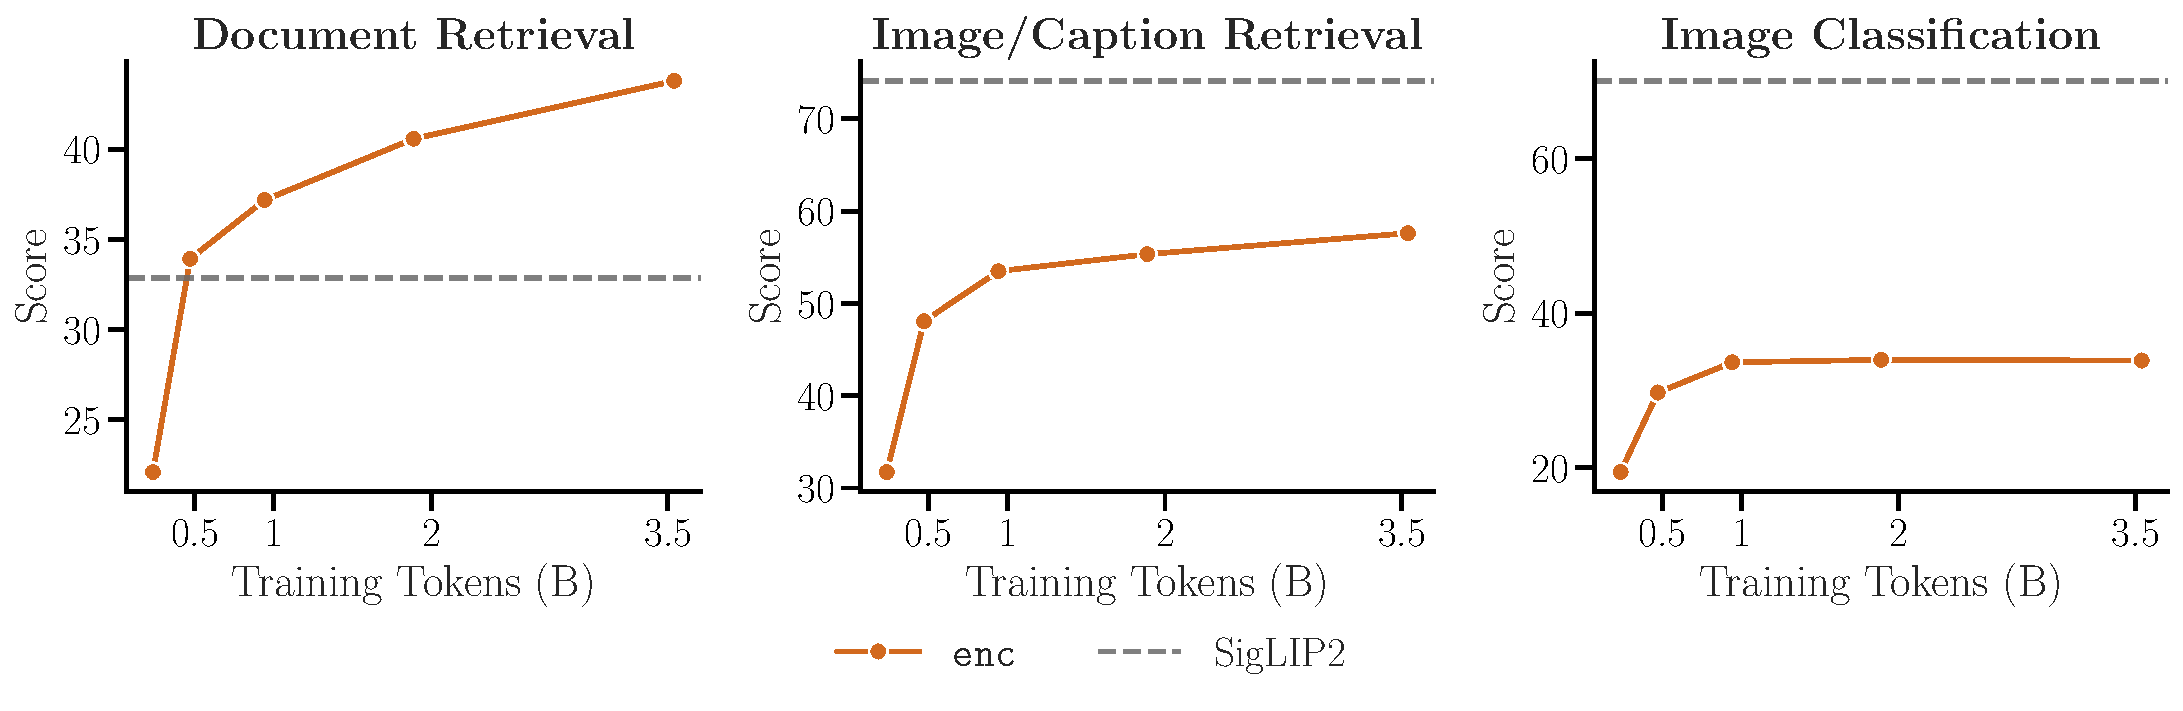
\includegraphics[width=0.95\textwidth]{images/modernvbert_figures/vbert_style/pt_scaling.pdf}
    \caption[Modality alignment scaling]{\textbf{Modality alignment scaling of early fusion encoders for up to 1 epoch (3.5B tokens) of data.} The dashed line indicates the vision encoder evaluated standalone without further training. Our findings show that retrieval tasks benefits from extended modality alignment phase, particularly in document retrieval, where performance quickly surpasses that of the standalone vision encoder. }
    % \manu{paul: could we have this in terms of B tokens seen instrad of steps ? remove average, increase fonts}}
    \label{fig:pt_scaling}
\end{figure}


\noindent\textbf{Bidirectional attention fully unlocks Late Interaction.}
Inspired by the effectiveness of bidirectional attention in text-only retrieval~\sidecite{gisserotboukhlef2025pretrainencodersmaskedlanguage, weller2025seqvsseqopen}\sidenote{\cite{chen2025mocamodalityawarecontinualpretraining} investigate post-hoc removal of the attention mask during visual retrieval fine-tuning.}, we investigate if it surpasses causal attention in \textit{visual document retrieval}, particularly when using the multi-vector late interaction matching common in SOTA visual retrievers~\sidecite{khattab2020colbert, faysse2025colpaliefficientdocumentretrieval}.
% Table~\ref{table:vidore_alignment_objective} presents the results on the ViDoRe benchmark suite when training a visual retriever with different attention masking and objective loss.  
Figure~\ref{fig:enc_dec_multivec} reports single vector and late interaction results on the ViDoRe benchmark for various model variants. On top of the standard \texttt{enc} (MLM) and \texttt{dec} (CLM) models, we evaluate the \texttt{dec-enc} and the  \texttt{dec} models modality aligned with MLM objectives to determine whether bidirectional attention capabilities can be obtained in later stages of training.

Single-vector embedding results are close between bidirectional and causal attention models for document retrieval, with \texttt{enc} slightly outperforming \texttt{dec} by +1.6 nDCG@5. 
% Single-vector embedding results are close between bidirectional and causal attention models, with \texttt{dec} slightly outperforming \texttt{enc}. 

Intuitively however, bidirectional attention makes a huge difference when used in late interaction settings, substantially exceeding the causal counterpart by +10.6 nDCG@5. 
% \paul{@MF recheck jai du changer car dec est legerement meilleur en single vec - ouais true que en doc}
Causal decoders are incapable of correctly contextualizing image or text token representations seen at the beginning of the sequences. \textit{This is a key result as almost all current visual retrievers, including late interaction variants, are causal models, clearly indicating some performance is left on the table.}

Removing the causal attention mask during training does not suffice to recover the \texttt{enc} late interaction performance at these data regimes. This indicates converting trained decoders as late interaction retrievers is highly non trivial, and confirms the insights from \sidecite{weller2025seqvsseqopen}; when possible, training encoder models from scratch remain better for retrieval tasks.



% \begin{table*}[ht]
%   \centering
%   \renewcommand{\arraystretch}{1.2}
%   \small
%   \resizebox{0.6\textwidth}{!}{%
%   \begin{tabular}{@{} >{}l cc >{\columncolor{avgcol}}c}
%     % Group banners with distinct colors, no top rule
    
%     % & \multicolumn{2}{>{\columncolor{grpA}}c}{\textbf{Doc. Retrieving}}  \\
%     % \cmidrule(lr){2-3}
%     & \rot{ViDoRe(v1)} & \rot{ViDoRe(v2)} 
%     & \rot{\textbf{Average}} \\
%     \midrule
%     \multicolumn{3}{@{}l}{\itshape Causal Base LM}\\
%     CLM Alignment & 67.1 & 41.4 & 54.3 \\
%     MLM Alignment & 65.6 & 35.1 & 50.4 \\
%     \hspace{3pt} + \textit{Base Model Annealing} & 67.4 & 38.9 & 53.1 \\
%     \midrule
%     \multicolumn{3}{@{}l}{\itshape Bidirectional Base LM}\\
%     MLM Alignment & \textbf{79.1} & \textbf{50.6} & \textbf{64.9}  \\
%     \bottomrule
%   \end{tabular}%
%   }
%   \caption{Scores (nDCG@5) of the models on ViDoRe v1 and ViDoRe v2 \textit{english} splits\footnote{Our base LM models are trained on english only, thus evaluating on multilingual splits for such comparison would be mostly noise.} when training a visual retriever with different attention masking and objective loss. \textit{Causal Base LM}  are the models based on a decoder LM, while \textit{Bidirectional Base LM} are the one from an encoder LM. \textit{Base Model Annealing} is the LM backbone annealed as an encoder \textbf{before modality alignment}.}
%   \label{table:vidore_alignment_objective}
% \end{table*}

% \textit{For a fixed model, image resolution is an important factor influencing downstream performance. We therefore examine how resolution impacts embedding tasks, and whether its effect varies by task type.}

\begin{figure*}[t]
    \centering

    \includegraphics[width=0.43\textwidth]{images/modernvbert_figures/enc_dec_vidore_palette.pdf}
    \caption[Attention mask impact]{\textbf{Impact of attention masks and training objectives on document retrieval performances.} 
    We report the average nDCG@5 on English splits of ViDoRe benchmarks for models post-trained on ColPali.
    % Employing native bidirectional attention outperforms the other approaches when used in multi-vector settings 
    }
    \label{fig:enc_dec_multivec}

\end{figure*}

\begin{figure*}[t]
    \centering

    \renewcommand{\arraystretch}{1.1}
    \small
    \resizebox{0.48\textwidth}{!}{%
    \begin{tabular}{@{} l c ccc >{\columncolor{avgcol}}c}
    & {HR Cooldown} & \rot{Document Retrieval} & \rot{Image/Caption Retrieval} & \rot{Image Classification} & \rot{\textbf{Average}} \\

    \midrule
    512px  & \xmark & 30.7 & \underline{58.8} & \textbf{41.4} & 43.6 \\
    1024px & \xmark & 42.2 & \textbf{58.9} & \underline{37.2} & \textbf{46.1} \\
    2048px & \xmark & \underline{43.8} & 57.6 & 33.9 & 45.1 \\
    2048px & \cmark & \textbf{45.8} & 57.8 & 33.7 & \underline{45.8} \\

    \bottomrule
    \end{tabular}%
    }
    \caption[Image resolution effect]{\textbf{Effect of image resolution on VL encoder abilities.} Document retrieval performance increases with higher image resolution. Further annealing the encoder on high-resolution images (HR Cooldown) at the end of modality alignment yields additional gains. By contrast, for non-document tasks, raising the resolution tends to degrade performance.}
    \label{table:image_resolution}

\end{figure*}

% \begin{figure*}[t]
%     \centering
%     % Left side: first figure (single subfigure kept)
%     \begin{minipage}{0.48\textwidth}
%         \centering
%         \includegraphics[width=0.9\textwidth]{images/modernvbert_figures/enc_dec_vidore_palette.pdf}
%         \caption{\textbf{Impact of attention masks and training objectives on document retrieval performances.} 
%         We report the average nDCG@5 on English splits of ViDoRe benchmarks for models post-trained on ColPali.
%         % Employing native bidirectional attention outperforms the other approaches when used in multi-vector settings 
%         } 
%         \label{fig:enc_dec_multivec}
%     \end{minipage}%
%     \hfill
%     % Right side: second figure + table
%     \begin{minipage}{0.48\textwidth}
%         \renewcommand{\arraystretch}{1.1}
%         \small
%         \resizebox{\textwidth}{!}{%
%         \begin{tabular}{@{} l c ccc >{\columncolor{avgcol}}c}
%         & {HR Cooldown} & \rot{Document Retrieval} & \rot{Image/Caption Retrieval} & \rot{Image Classification} & \rot{\textbf{Average}} \\
    
%         \midrule
%         512px & \xmark & 30.7 & \underline{58.8} & \textbf{41.4} & 43.6 \\
%         1024px & \xmark & 42.2 & \textbf{58.9} & \underline{37.2} & \textbf{46.1} \\
%         2048px & \xmark & \underline{43.8} & 57.6 & 33.9 & 45.1 \\
%         2048px & \cmark & \textbf{45.8} & 57.8 & 33.7 & \underline{45.8} \\
        
%         \bottomrule
%         \end{tabular}%
%         }
%         \captionof{table}{\textbf{Effect of image resolution on VL encoder abilities.} Document retrieval performance increases with higher image resolution. Further annealing the encoder on high-resolution images (HR Cooldown) at the end of modality alignment yields additional gains. By contrast, for non-document tasks, raising the resolution tends to degrade performance.}
%         \label{table:image_resolution}
            
%         % \vspace{1em}
%         % \centering        \includegraphics[width=0.9\linewidth]{images/modernvbert_figures/pt_scaling.png}
%         % \captionof{figure}{\textbf{Pretraining phase scaling.} The dashed line marks the vision tower baseline. \paul{TODO: I wait to fix what tiles we show here before writting the caption(mean of tasks per domain like above, or per task)}}
%         % \label{fig:pt_scaling}
%     \end{minipage}
% \end{figure*}


% However, we also observe a negative correlation with performance on tasks that involve natural images. This suggests that the multiple high-resolution crops generated during preprocessing may obscure global separable features necessary for classification, and that passing one image in the size expected by the vision tower is optimal. 
%These results highlight the importance of flexible, resolution-aware preprocessing pipelines that can adapt hierarchically to the native resolution of each input image.

% \begin{table*}[t]
%   \centering
%   \renewcommand{\arraystretch}{1.2}
%   \small
%   \resizebox{0.5\textwidth}{!}{%
%   \begin{tabular}{@{} l c ccc >{\columncolor{avgcol}}c}
%     & {HR Cooldown} & \rot{Document Retrieval} & \rot{Caption Retrieval} & \rot{Zero-Shot Classification} & \rot{\textbf{Average}} \\

%     \midrule
%     512px & \xmark & 30.7 & 58.8 & 45.1 & 44.9 \\
%     1024px & \xmark & 42.2 & \textbf{58.9} & 42.8 & \textbf{48.0} \\
%     2048px & \xmark & 43.8 & 57.6 & 40.4 & 47.3 \\
%     2048px & \cmark & \textbf{45.8} & 57.8 & 39.2 & 47.6 \\
    
%     \bottomrule
%   \end{tabular}%
%   }
%   \caption{\textbf{Effect of image resolution on VL encoder abilities.} Document retrieval performance increases with higher image resolution. Further annealing the encoder on high-resolution images (HR Cooldown) during pretraining yields additional gains. By contrast, for non-document tasks, raising the resolution tends to degrade performance.}
%   \label{table:image_resolution}
% \end{table*}

% \begin{table*}[t]
%   \centering
%   \renewcommand{\arraystretch}{1.1}
%   \small
%   \resizebox{\textwidth}{!}{%
%   \begin{tabular}{@{} l cc ccc >{\columncolor{avgcol}}c}
%     & {HR Cooldown} & {Resize at Inference} & \rot{Document Retrieval} & \rot{Caption Retrieval} & \rot{Zero-Shot Classification} & \rot{\textbf{Average}} \\

%     \midrule
%     512px & \xmark & \cmark & 30.7 & 58.8 & 45.1 & 44.9 \\
%     1024px & \xmark & \cmark & 42.2 & \textbf{58.9} & 42.8 & 48.0 \\
%     2048px & \xmark & \cmark & 43.8 & 57.6 & 40.4 & 47.3 \\
%     2048px & \cmark & \cmark & \textbf{45.8} & 57.8 & 39.2 & 47.6 \\
%     2048px & \xmark & \xmark & 42.6 & 56.0 & \textbf{46.7} & \textbf{48.5} \\
    
%     \bottomrule
%   \end{tabular}%
%   }
%   \caption{\textbf{Effect of image resolution on VL encoder abilities.} Document retrieval performance increases with higher image resolution. Further annealing the encoder on high-resolution images (HR Cooldown) during pretraining yields additional gains. By contrast, for non-document tasks, raising the resolution tends to degrade performance, with best average score achieved when not resizing the input images during inference.}
%   \label{table:image_resolution}
% \end{table*}

\subsection{Contrastive Training Design} 

The previous subsection established bidirectional encoder models to often be the best option when training visual retrievers. In the following experiments, we assess contrastive training choices and only report results for the encoder model for simplicity.

% After the first stage, the model can perform token prediction, but its latent space is not optimized for general concept embeddings. A common solution is to add a second stage with a contrastive objective~\sidecite{jiang2024vlm2vectrainingvisionlanguagemodels, jiang2024e5vuniversalembeddingsmultimodal, chen2025mme5improvingmultimodalmultilingual, chen2025mocamodalityawarecontinualpretraining}.  
% This stage aligns concept representations across modalities at the sentence level, yielding models well suited for zero-shot tasks~\sidecite{radford_learning_2021, zhai_sigmoid_2023}.  
% \paul{Un truc style on a vu avant que token-level c'est bien pour documentaire masi CL aide sur le reste. On regarde comment on peut scale notre dataset pour tirer un max de perf across all tasks} In this section, we search for the most effective contrastive post-training mix to draw maximum capabilities. 

% \textit{While additional paired data are required to close the performance gap on natural image tasks, such resources remain limited. This raises the question of how alternative data sources might be leveraged to address this gap.}


\noindent\textbf{Image resolution benefits are task-specific.} 
Image resolution plays a critical role in VLM generative capabilities, notably in document-focused tasks, as higher-resolution inputs enables the model to capture finer visual cues~\sidecite{hu2024mplugdocowl2highresolutioncompressingocrfree, marafioti2025smolvlmredefiningsmallefficient}.
%We examine how these resolution dynamics transfer to embedding tasks. 
Modality alignment is done at a fixed image resolution of 1024 pixels (longer side) and we report scores of contrastive training runs with varying settings in Table~\ref{table:image_resolution}. To vary the resolution, images of the highest quality available are scaled to the desired size (often downscaled) before being fed to the image tokenizer. Our findings confirm that embedding tasks are strongly sensitive to image-resolution. In particular, \textit{training with higher resolution inputs substantially improves the results on visual document retrieval benchmarks}, consistent with prior work in generative settings~\cite{beyer2024paligemmaversatile3bvlm, mckinzie_mm1_2024}. Furthermore, adding a cool-down phase by showing higher-resolution images towards the end of the modality alignment phase yields additional gains. This suggests that models can adapt their attention mechanisms to finer details when exposed to increased resolution. Interestingly, these findings do not hold in natural image tasks, where high resolution can even degrade performance.


% \noindent\textbf{Scaling the modality alignment phase for better token representations.}  
% Prior work shows that scaling the CLM modality alignment phase of VLMs improves their generative abilities~\sidecite{beyer2024paligemmaversatile3bvlm, mckinzie_mm1_2024, wang2024qwen2vlenhancingvisionlanguagemodels}. We test whether similar gains hold in a retrieval setting by evaluating checkpoints during modality alignment with an MLM objective, for up to 3.5B tokens. Figure~\ref{fig:pt_scaling} illustrates the results of the post-trained checkpoints on diverse tasks. 
% The model consistently improves across all retrieval tasks with an increasing amount of alignment data. This is similar to what is observed for generative tasks, suggesting that the model learns to create richer token representations with the information available in the images during this modality alignment stage.

% \begin{figure}[t]
%     \centering    \includegraphics[width=0.95\textwidth]{images/modernvbert_figures/pt_scaling.png}
%     \caption{\textbf{Modality alignment scaling.} The dashed line marks the vision tower baseline. \paul{TODO: I wait to fix what tiles we show here before writing the caption(mean of tasks per domain like above, or per task)}}
    
%     \label{fig:pt_scaling}
% \end{figure}

% \begin{figure}[t]
%     \centering    \includegraphics[width=0.85\textwidth]{images/modernvbert_figures/finegrain/pt_scaling.png}
%     \caption{Pretraining phase scaling. The dashed
% line marks the vision tower baseline. \paul{TODO: I wait to fix what tiles we show here before writing the caption(mean of tasks per domain like above, or per task)}}
    
%     \label{fig:pt_scaling_finegrain}
% \end{figure}

% \begin{table*}[b]
%   \centering
%   \renewcommand{\arraystretch}{1.2}
%   \small
%   \resizebox{\textwidth}{!}{%
%   \begin{tabular}{@{} >{}l c c c >{\columncolor{avgcol}}c}
%     & {Document Retrieval} & {Caption Retrieval} & {Zero-Shot Classification} & {\textbf{Average}} \\

%     \midrule
%     Baseline CL Mix & 43.9 & \textbf{57.2} & 40.6 & 47.2 \\
%     + \textit{Text$\rightarrow$Text Pairs} & 45.6 & 53.2 & 42.3 & 47.0 \\
%     + \textit{Image$\rightarrow$Caption Pairs} & \textbf{45.8} & 54.4 & \textbf{44.4} & \textbf{48.2} \\
    
%     \bottomrule
%   \end{tabular}%
%   }
%   \caption{\textbf{Impact of contrastive post-training mixtures on downstream tasks.} Incorporating text-only pairs improves performance on document retrieval, but degrades other performances. Adding natural images-captions pairs substantially enhances performance on zero-shot classification tasks.}
%   \label{table:cl_mix_impact}
% \end{table*}

\begin{table*}[b]
  \centering
  \renewcommand{\arraystretch}{1.4}
  \small
  \resizebox{\textwidth}{!}{%
  \begin{tabular}{@{} >{}l  ccc >{\columncolor{avgcol}}c}
    & {Document Retrieval} & {Image/Caption Retrieval} & {Image Classification} & {\textbf{Average}} \\

    \midrule
    Baseline CL Mix & 43.9 & \textbf{57.2} & 36.1 & 45.7 \\
    + \textit{Text$\rightarrow$Text Pairs} & 45.6 & 53.2 & 35.7 & 44.8 \\
    + \textit{Image$\rightarrow$Caption Pairs} & \textbf{45.8} & 54.4 & \textbf{49.9} & \textbf{50.0} \\
    
    \bottomrule
  \end{tabular}%
  }
  \caption[Contrastive training mixtures impact]{\textbf{Impact of contrastive training mixtures on downstream tasks.} Incorporating text-only pairs improves performance on document retrieval, but degrades other performances. Adding natural images-captions pairs substantially enhances performance on classification tasks.}
  \label{table:cl_mix_impact}
\end{table*}


\noindent\textbf{Increasing the pool of contrastive pairs.}
\label{sec:scaling=-cont}
% \quentin{A series of ablation studies on our post-training data composition revealed two key insights. First, incorporating unimodal text-only pairs from \cite{thakur2025rlhn} markedly enhances performance on visual document retrieval \ref{table:cl_mix_impact}. We attribute this enhancement to the model learning a more complex semantic understanding from the textual data, which successfully transfers across modalities to the image-text task. Second, we found that adding the \natcap{} dataset is crucial for preserving the model's general vision capabilities. By expanding the contrastive dataset and increasing the variety of image types, it effectively counteracts the performance degradation on image classification benchmarks typically seen when aligning the original SigLIP baseline with our text encoder.}
A severe limitation that current visual retrievers face is the lack of large volumes of high quality (document image, query pairs). 
Previous work \sidecite{ma2024unifyingmultimodalretrievaldocument, faysse2025colpaliefficientdocumentretrieval, jiang2024vlm2vectrainingvisionlanguagemodels, zhang2025gmeimprovinguniversalmultimodal} has relied on a mix of repurposed existing visual question answering datasets and synthetically generated queries with external LLMs. Even put together however, the field is only a year old, and these datasets remain small in size and often of poor quality.


% As described in Section ~\ref{sec:ablation_tasks}, using modality alignment is only one phase of training stage reduces performance in natural image tasks compared to the vision tower backbone. This underscores the need for extensive contrastive post-training to obtain stronger single-vector representations~\sidecite{radford_learning_2021}. 
% \paul{on peut affiner la motiv}
% However, the absence of large-scale and high-quality multimodal contrastive datasets constrains the scalability of this phase. To address this, we investigate whether incorporating additional data sources incrementally can mitigate these limitations. 
A central question in our study is whether the abundance of \emph{text-only} query–document pairs can be exploited to improve \emph{visual} retrieval via cross-modal capability transfer. To probe this, we run contrastive training under three regimes. Unlike prior work that “warms up” visual retrievers or trains exclusively with text-only pairs \sidecite{ma2024unifyingmultimodalretrievaldocument, jiang2024e5vuniversalembeddingsmultimodal}, we \emph{interleave} text-only pairs and text–image pairs throughout training at a 1:1 ratio. The dataset sources are detailed in Appendix~\ref{appendix:contrastive_mix}

As reported in Table~\ref{table:cl_mix_impact}, incorporating text-only pairs yields a sizeable improvement on visual document retrieval (+1.7 \textsc{nDCG}@5), indicating clear cross-modal transfer—likely facilitated by the backbone’s jointly learned text–image embedding space. This result suggests that domain-specific training corpora can be assembled irrespective of native modality, reducing duplication of effort and lowering data-collection costs.

We further evaluate training with \natcap{}, a corpus of natural images paired with synthetic, highly detailed captions (see Appendix~\ref{appendix:natcap}). This scaling step improves downstream performance across the board—most notably on natural-image tasks, and with a smaller but consistent gain on document retrieval (+0.2 \textsc{nDCG}@5). Together, these findings underscore the importance of scaling contrastive learning with high-quality data, but which doesn't need to be exclusively image document focused.


% \begin{table*}[t]
%   \centering
%   \renewcommand{\arraystretch}{1.2}
%   \small
%   \resizebox{\textwidth}{!}{%
%   \begin{tabular}{@{} >{}l cccc >{\columncolor{avgcol}}c}

%     & Document Retrieval & Captioning & Classification (0S) & Classification (LP)
%     & \textbf{Average} \\

%     \toprule
%     % \multicolumn{6}{@{}l}{\itshape Single-Vector} \\
%     % ColPali & -- & -- & -- & -- & -- \\
%     % \hspace{3pt} + \textit{MSCOCO} & 43.9 & \textbf{57.2} & 19.8 & 52.2 & 43.3 \\
%     Baseline CL mix & 43.9 & \textbf{57.2} & 19.8 & 52.2 & 43.3 \\
%     \hspace{3pt} + \textit{\natcap{}} & \underline{44.9} & 53.7 & \underline{36.2} & \underline{59.8} & 48.7 \\
%     \hspace{3pt} + \textit{Text$\rightarrow$Text Data}& \textbf{45.8} & \underline{54.4} & \textbf{39.8} & \textbf{60.0} & \textbf{50.0} \\
%     % \midrule
%     % \multicolumn{6}{@{}l}{\itshape Multi-Vector} \\
%   \end{tabular}%
%   }
%   \caption{Impact of contrastive post-training mixtures on downstream tasks. Adding \natcap{} substantially enhances performance on image classification tasks, but leads to a decrease in performance on natural image captioning. Incorporating unimodal text data improves performance on document retrieval  and zero-shot tasks.}
%   \label{table:cl_mix_impact}
% \end{table*}

% \begin{table*}[h]
%   \centering
%   \renewcommand{\arraystretch}{1.2}
%   \small
%   \resizebox{\textwidth}{!}{%
%   \begin{tabular}{@{} >{}l ccc >{\columncolor{avgcol}}c}

%     & \rot{Document Retrieval} & \rot{Caption Retrieval} & \rot{Zero-Shot Classification}
%     & \rot{\textbf{Average}} \\

%     \toprule
%     % \multicolumn{6}{@{}l}{\itshape Single-Vector} \\
%     % ColPali & -- & -- & -- & -- & -- \\
%     % \hspace{3pt} + \textit{MSCOCO} & 43.9 & \textbf{57.2} & 19.8 & 52.2 & 43.3 \\
%     Baseline CL mix & 43.9 & \textbf{57.2} & \underline{19.8} & \underline{40.3} \\
%     \hspace{3pt} + \textit{Text$\rightarrow$Text Pairs (RLHN)}& \underline{45.6} & 53.2 & 18.2 & 39.0 \\
%     % \hspace{3pt} + \textit{\natcap{}} & \underline{44.9} & 53.7 & \underline{36.2} & 44.9 \\
%     \hspace{3pt} + \textit{Image$\rightarrow$Caption Pairs (\natcap{})} & \textbf{45.8} & \underline{54.4} & \textbf{39.8} & \textbf{46.7} \\
%     % \midrule
%     % \multicolumn{6}{@{}l}{\itshape Multi-Vector} \\
%     \bottomrule
%   \end{tabular}%
%   }
%   \caption{\textbf{Impact of contrastive post-training mixtures on downstream tasks.} Incorporating unimodal text data improves performance on document retrieval, but degrades other performances. Adding \natcap{} substantially enhances performance on zero-shot classification tasks.}
%   \label{table:cl_mix_impact}
% \end{table*}



% \noindent\textbf{Merging Models.} 

% \begin{table*}[t]
%   \centering
%   \renewcommand{\arraystretch}{1.2} % Adjusts row spacing for better readability
%   \small % Use a smaller font size for the table
%   % Resize the table to fit the width of the text area
%   \resizebox{\textwidth}{!}{%
%   \begin{tabular}{@{} l l c cc cc c @{}} % Column formatting
%     % --- Column Headers with Grouping and Colors ---
%     &
%     & \multicolumn{1}{>{\columncolor{grpA}}c}{\textbf{Captioning}}
%     & \multicolumn{2}{>{\columncolor{grpB}}c}{\textbf{Doc. Retrieval}}
%     & \multicolumn{2}{>{\columncolor{grpC}}c}{\textbf{Natural Image}}
%     & \multicolumn{1}{>{\columncolor{grpD}}c}{\textbf{Other}} \\
    
%     % Use cmidrule for partial lines under the main groups
%     \cmidrule(lr){3-3} \cmidrule(lr){4-5} \cmidrule(lr){6-7} \cmidrule(lr){8-8}
    
%     % --- Sub-headers for specific datasets/tasks ---
%     Task & Model & Image Captioning & ViDoRe(v1) & ViDoRe(v2) & MSCOCO & Flickr30k & Others \\
%     \midrule
    
%     % --- Table Data ---
%     % Using \texttt{} for model names to correctly display underscores and improve readability
%     4 & \texttt{baseline\_x\_baseline-\natcap{}-text-2\_t075} & 0.576 & 0.484 & 0.136 & 0.478 & 0.674 & 0.898 \\
%     0 & \texttt{baseline\_x\_baseline-\natcap{}-text-05}     & 0.561 & 0.483 & 0.138 & 0.466 & 0.656 & 0.901 \\
%     1 & \texttt{baseline\_x\_baseline-\natcap{}-text-2}      & 0.561 & 0.480 & 0.132 & 0.467 & 0.655 & 0.900 \\
%     5 & \texttt{baseline\_x\_baseline-text-07\_x\_...-\natcap{}} & 0.544 & 0.469 & 0.125 & 0.451 & 0.637 & 0.901 \\
%     2 & \texttt{baseline\_x\_baseline-\natcap{}-text-2\_avg}  & 0.551 & 0.462 & 0.129 & 0.450 & 0.653 & 0.898 \\
%     3 & \texttt{baseline\_x\_baseline-\natcap{}-text-2\_t025} & 0.537 & 0.466 & 0.127 & 0.446 & 0.628 & 0.900 \\
%     \bottomrule
%   \end{tabular}%
%   }
%   \caption{Performance comparison of different model configurations across a variety of downstream tasks. The table evaluates performance on image captioning, document retrieval (ViDoRe), natural image tasks (MSCOCO, Flickr30k), and other benchmarks.}
%   \label{table:model_performance_comparison}
% \end{table*}

\section{Building a Small yet Mighty Visual Retriever.}
% \noindent\textbf{Assymetric encoders.} 
% \noindent\textbf{Ensembled embeddings.} 

% \manu{Maybe we can take the kaobox takeaway style a bit similar to here ? \url{https://arxiv.org/pdf/2410.10781}}
% \noindent\textbf{Selecting the right recipe.} Putting together the results from our experiment, we devise a training recipe for a small visual document retriever. 

% Our ablation studies yields key insights on training early fusion visual encoders. 
% Notably, practitioners should select architectures according to task needs: fused VLMs are preferable for document tasks due to their ability to generate token-level representations, whereas lightweight CLIP-style ViTs offer superior sentence-level alignment particularly useful in image captioning and classification. When building visual document retrievers from scratch, practitioners should prioritize bidirectional attention to fully exploit the benefits of a token-level alignment with late interaction.
% When starting from pretrained models and larger parameter scales, we suggest annealing causal VLMs into bi-directional encoders using methods such as MoCa~\sidecite{chen2025mocamodalityawarecontinualpretraining}. This strategy combines the advantages of bi-directional attention in late interaction with the rich semantic and world knowledge captured during large-scale causal pretraining.

% \paul{Linking stuff: We want to build a visual document retriever from scratch, freeing ourselves from the constraint of repurposing a VLM. Building on our insights, [...].}

\subsection{Training.} 

\noindent\textbf{Recipe.} Putting together the results from our experiments, we devise a training recipe for a small visual document retriever \flagship{}. It combines a state-of-the-art 150M text bidirectional encoder~\sidecite{weller2025seqvsseqopen} with the ModernBERT architecture \sidecite{modernbert} and a small vision encoder SigLIP2-16B-512 of 100M parameters~\sidecite{tschannen2025siglip2multilingualvisionlanguage}. We modality align both models with a MLM objective for 10B tokens, 3 times longer than during our experiments. To boost document understanding, we augment the input image resolution from 1024px to 2048px during a modality alignment cooldown stage (2B tokens). We call the resulting model \flagship{}.
%In line with our results, we  scale the post-training corpus to 
% \manu{we don't care about the bimodell - only describe the setup for the colmodel. ModernVBert is a multivector model, Bi doesn't exist (except appendix)}
%pairs, resulting in the mixture summarized in Table~\ref{tab:final_cl_mix} and train with Late Interaction objectives.  F
Following the findings of Section~\ref{sec:scaling=-cont}, we then scale the contrastive training mix from previous experiments to combine document–query pairs with text-only pairs, and use 1 hard negatives for each document-query pair and 2 for each text-only pairs. We opt for a 2/1 text-to-image ratio following our ablation results introduced in Appendix~\ref{appendix:text_image_ratio}. This results in \colflagship{}, a compact late interaction model. For reference, we also train \textit{Bi}\flagship{}, a single vector variant. More training details are provided in Appendix~\ref{appendix:implementation_details}.

% \begin{table*}[h]
% \centering
% \setlength{\tabcolsep}{6pt}
% \renewcommand{\arraystretch}{1.15}
% \begin{tabular}{l r}
% \toprule
% \textbf{Source} & \textbf{Contrastive Pairs} \\
% \midrule
% ColPali~\sidecite{faysse2025colpaliefficientdocumentretrieval}                          & 118 000 \\
% MSCOCO~\sidecite{lin_microsoft_2014}                            & 118 000 \\
% \natcap~\textit{(ours)}           & 118 000 \\
% RLHN~\sidecite{thakur2025rlhn}                              & 680 000 \\
% \midrule
% \textbf{TOTAL}                    & \textbf{1 020 000} \\
% \bottomrule
% \end{tabular}
% \caption{\manu{This takes a shit ton of space - is it useful ?}}
% \label{tab:final_cl_mix}
% \end{table*}

% new mix, add if concluant
% \begin{table*}[h]
% \centering
% \setlength{\tabcolsep}{6pt}
% \renewcommand{\arraystretch}{1.15}
% \begin{tabular}{l r}
% \toprule
% \textbf{Source} & \textbf{Contrastive Pairs} \\
% \midrule
% ColPali~\sidecite{faysse2025colpaliefficientdocumentretrieval}                          & 118 000 \\
% VDR                               & 240 000 \\
% MSCOCO (3 captions)               & 354 000 \\
% \natcap~\textit{(ours)}           & 333 000 \\
% RLHN                              & 680 000 \\
% \midrule
% \textbf{TOTAL}                    & \textbf{1 725 000} \\
% \bottomrule
% \end{tabular}
% \caption{\paul{@QM check this and comment and cite everybody}.}
% \label{tab:final_cl_mix}
% \end{table*}



% \noindent\textbf{Evaluation.}  
% We evaluate our approach on the ViDoRe benchmark suite~\sidecite{faysse2025colpaliefficientdocumentretrieval, macé2025vidorebenchmarkv2raising}\footnote{We only report the English splits as the base model is mainly efficient in English tasks}. We compare our approach against CLIP encoders~\sidecite{radford_learning_2021, zhai_sigmoid_2023}, as well as recent VLMs repurposed for embedding tasks~\sidecite{jiang2024vlm2vectrainingvisionlanguagemodels, meng2025vlm2vecv2advancingmultimodalembedding, chen2025mocamodalityawarecontinualpretraining} and similar early fusion encoders~\sidecite{zhou2024vistavisualizedtextembedding} on tasks. Furthermore, we evaluate \colflagship{}–the document-optimized version of our \flagship{}– against the retrievers of the ViDoRe leaderboard~\sidecite{faysse2025colpaliefficientdocumentretrieval, macé2025vidorebenchmarkv2raising}. We present the baselines in detail in Appendix~\ref{appendix:baselines}

\subsection{Results.}
\label{sec:results}

\begin{table*}[t]
  \centering
  \renewcommand{\arraystretch}{1.03}
  \small
  \resizebox{\textwidth}{!}{%
  \begin{tabular}{@{} >{}l cc cc >{\columncolor{avgcol}}c >{\columncolor{latcol}}c}
    & {Late Interaction} & {Model Size (B)} & \rot{ViDoRe(v1)} & \rot{ViDoRe(v2,eng)} & \rot{\textbf{Average}} & \rot{\textbf{Latency (ms)}} \\

    \midrule
    \multicolumn{7}{@{}l}{\itshape $\ge$ 1B Parameters}\\
    MoCa-3B~\cite{chen2025mocamodalityawarecontinualpretraining}            &  & 3.75 & 80.1 & 53.8 & 66.9 & 158 \\    VLM2Vec~\cite{jiang2025vlm2vectrainingvisionlanguagemodels}             &  & 4.15 & 49.8 & 36.5 & 43.1 & 211 \\
    GME-Qwen2~\cite{zhang2025gmeimprovinguniversalmultimodal}               &  & 8.29 & 89.9 & 61.8 & 75.8 & 412\\
    E5-V~\cite{jiang2024e5vuniversalembeddingsmultimodal}                   &  & 8.36 & 62.7 & 49.4 & 56.1 & 434 \\
    % llama-nemoretriever-colembed-1b                                          & \cmark & 2.42 & -    & 90.5 & 65.7 & 78.1 & - \\
    % colpali-v1.3                                                             & \cmark & 2.92 & -    & 84.8 & 56.1 & 70.4 & - \\
    ColPali~\cite{faysse2025colpaliefficientdocumentretrieval}              & \cmark & 2.92 & 81.6 & 56.8 & 69.2 & 175 \\
    ColQwen2.5~\cite{faysse2025colpaliefficientdocumentretrieval}           & \cmark & 3.75 & 89.5 & 61.5 & 75.5 & 158 \\
    Jina-v4~\cite{günther2025jinaembeddingsv4universalembeddingsmultimodal} & \cmark & 3.75 & 90.4 & 60.1 & 75.2 & 158 \\
    NemoRetriever-3B~\cite{xu2025llamanemoretrievercolembedtopperforming}   & \cmark & 4.40 & 91.0 & 66.3 & 78.7 & 155 \\

    \midrule
    \multicolumn{7}{@{}l}{\itshape $\le$ 1B Parameters}\\
    Jina CLIP$^*$~\cite{koukounas_jina_2024}                                    &  & 0.22 & 17.6 & 14.0 & 15.8 & \textbf{14} \\
    BGE Visualized M3$^*$~\cite{zhou2024vistavisualizedtextembedding}           &  & 0.87 & 12.4 & 10.2 & 11.3 & 38 \\
    SigLIP2-L-512/16$^*$~\cite{tschannen2025siglip2multilingualvisionlanguage}  &  & 0.88 & 43.8 & 27.0 & 35.4 & 25 \\
    ColFlor~\cite{masrycolflor}                                             & \cmark & 0.17 & 68.8 & 43.0 & 55.9 & 17 \\
    % colSmol-256M                                                             & \cmark & 0.26 & 79.7 & 50.0 & 64.8 & - \\
    % colSmol-500M                                                             & \cmark & 0.50 & 82.5 & 52.1 & 67.3 & - \\
    \biflagship{} (ours)                                           &  & 0.25 & 63.6 & 35.7 & 49.7 & 20 \\
    \textbf{\colflagship{} (ours)}                                           & \cmark & 0.25 & \textbf{81.2} & \textbf{56.0} & \textbf{68.6} & 20 \\
    
    \bottomrule
  \end{tabular}%
   }
  \caption[Performance on ViDoRe]{\textbf{Performance on ViDoRe.}
  Our model \colflagship{} offers the best performance-size tradeoff, significantly outperforming existing sub-1B models and matching the performance of models up to 10x larger with substantially lower inference CPU latency. Details and GPU latencies in Appendix \ref{appendix:gpu_latency}. Models marked with $^*$ are not specifically trained for VDR. Bold values indicate the best performance amongst sub-1B models.}
  \label{table:res}
\end{table*}


\noindent\textbf{\colflagship{}}. The resulting model, \colflagship{} showcases strong performances on visual document retrieval benchmarks, especially relative to its size category (Figure~\ref{fig:pareto_vidore}). Despite having over 10 times less parameters than models such as ColPali released only a year ago, it is only 0.6 nDCG@5 points below on the aggregated ViDoRe benchmark scores (\autoref{table:res}). It also edges many larger single-vector repurposed VLM models released within the year \sidecite{chen2025mocamodalityawarecontinualpretraining, jiang2024e5vuniversalembeddingsmultimodal, jiang2024vlm2vectrainingvisionlanguagemodels}. It however falls short of top model performance on ViDoRe which are built on larger decoder VLMs pretrained and aligned on billions of tokens of text and image data.

Most sub-1B parameter models evaluated on document retrieval benchmarks are dual encoder models, since early fusion generative models that perform well are not common at this scale. The most related model is a 176M late interaction model, ColFlor \sidecite{masrycolflor}, trained from the Florence2 model \sidecite{xiao2023florence2advancingunifiedrepresentation}. ColFlor is 12.7 nDCG@5 points under \colflagship{}. \colflagship{} also largely outperforms off-the-shelf dual encoders, even when those have substantially larger parameter counts. 
These results highlights the benefits of multi-phase training and early fusion architectures for multi-modal document related tasks, even at smaller parameter counts. We also attribute the strong performance of \colflagship{} at smaller model sizes to the symbiosis of native bidirectional attention and Late Interaction matching, which largely boosts performance relative to comparable decoder models (Section~\ref{sec:ablation_tasks}).

%Our single-vector variant also sets a new optimal performance-size balance in among single-vector models, only beaten by GME-Qwen2 and MoCa-3B, that rely on much larger and more powerful base models. This confirms the soundness of our training approach, showcasing meaningful gains even without the Late Interaction paradigm.

\noindent\textbf{Speed.} As noted by \sidecite{xiao2025metaembedscalingmultimodalretrieval}, multi-vector visual retrievers are not bottlenecked in their inference speed by the late interaction matching operation, but rather by the latency required to encode queries with the text model. Our model demonstrates that strong performance is not incompatible with speed, even when running inference on consumer CPUs, which is the standard setting in most industrial local deployments of text embedding models. Latencies are computed by averaging query encoding times of all NanoBEIR queries, which are 23.4 word and 147.5 character long on average, and are run with batch size 1 to replicate online use cases. To prevent RAM bottlenecks, we benchmark on very high RAM (2TB) CPU cloud environments, but note models larger than 3B parameter require more than 12 GB RAM to run optimally.\sidenote{With more standard CPU RAM settings such as those found in low-end servers or Google Colab (12GB RAM), models above 3B parameters must rely on memory offloading to run, which adds up to dozens of seconds of latency per query.}  (\autoref{table:res}). \flagship{} achieves more than a 7x speedup on CPU over models with similar performances on ViDoRe. We further report model latency results on GPU hardware in Appendix~\ref{appendix:gpu_latency}. We notably demonstrate that with batched inference, \flagship{} based query encoders are able to encode 5000 queries per second on Nvidia H100 GPUs. ModernVBert's small model size also enables efficient batching when encoding documents. 


% \begin{table*}[t]
%   \centering
%   \renewcommand{\arraystretch}{1.2}
%   \small
%   \resizebox{\textwidth}{!}{%
%   \begin{tabular}{@{} >{}l cc cc >{\columncolor{avgcol}}c}
%     & {Model Size} & {Latency (ms)} & \rot{ViDoRe(v1)} & \rot{ViDoRe(v2)} & \rot{\textbf{Average}} \\

%     \midrule
%     \multicolumn{6}{@{}l}{\itshape Single-Vector Models}\\    
%     bge-visualized-m3 & 873M & - & 12.4 & 10.2 & 11.3 \\
%     siglip2-large-patch16-512 & 882M & - & 43.8 & 27.0 & 35.4 \\
%     VLM2Vec-Full & 4150M & - & 49.8 & 36.5 & 43.1 \\
%     MoCa-Qwen25VL-3B & 3750M & - & 80.1 & 53.8 & 66.9 \\
%     \textbf{\biflagship{}} & 252M & - & 63.6 & 35.7 & 49.7 \\
%     \midrule
%     \multicolumn{6}{@{}l}{\itshape Multi-Vector Models}\\
%     ColFlor & 174M & - & 68.8 & 43.0 & 55.9 \\
%     colSmol-256M & 256M & - & 79.7 & 50.0 & 64.8 \\
%     colSmol-500M & 500M & - & 82.5 & 52.1 & 67.3 \\
%     colpali-v1.1 & 2920M & - & 81.6 & 56.8 & 69.2 \\
%     colqwen2.5-v0.2 & 3000M & - & 89.5 & 61.5 & 75.5 \\
%     \textbf{\colflagship{}} & 252M & - & 81.2 & 56.0 & 68.6 \\
    
%     \bottomrule
%   \end{tabular}%
%   }
%   \caption{\textbf{ViDoRe Leaderboard.} Our model \colflagship{} offers the best performance-size tradeoff, matching the performance of models up to 10x larger. \paul{Do we report bi modernvbert?} \manu{please add colflor, colpali, colqwen, along with the parameter counts. structure this table with what we want to claim. perhaps don't show the biencoder results but only the Late Interaction results, the whole point of having an encoder might be to boost the number 1 way to boost vision retrievers, aka LI, this is not a sidething... We are trying to claim the best way to do things is with LI and it gets a disporoportionate boost when strating from encoders. Compare with LI, we don't care about the biencoder. Reorganoze models by param count (<1B, >1B, and then in these cats, you can have other categories. We need to be first in our category. Rethink how to highlight doc performance.}}
%   \label{tab:vidore_results}
% \end{table*}

% \begin{table*}[h]
% \centering
% \setlength{\tabcolsep}{6pt}
% \renewcommand{\arraystretch}{1.15}
% \begin{tabular}{l r}
% \toprule
% \textbf{Source} & \textbf{Contrastive Pairs} \\
% \midrule
% ColPali~\sidecite{faysse2025colpaliefficientdocumentretrieval}                          & 118 000 \\
% MSCOCO~\sidecite{lin_microsoft_2014}                            & 118 000 \\
% \natcap~\textit{(ours)}           & 118 000 \\
% RLHN~\sidecite{thakur2025rlhn}                              & 680 000 \\
% \midrule
% \textbf{TOTAL}                    & \textbf{1 020 000} \\
% \bottomrule
% \end{tabular}
% \caption{\manu{This takes a shit ton of space - is it useful ?}}
% \label{tab:final_cl_mix}
% \end{table*}




\section{Related Work}

% \noindent\textbf{Contrastive Vision Language Models.}  
% Early multimodal representation learning approaches mapped latent representations of text and images into a shared space by aligning disjoint encoders through contrastive learning~\sidecite{radford_learning_2021, zhai_sigmoid_2023}. These models laid the foundation for visual embedding tasks such as classification and image caption retrieval. However, they are not optimized for applications that require deeper visual document understanding, as they lack token-level cross-modality alignment objectives and face architectural limitations~\sidecite{faysse2025colpaliefficientdocumentretrieval, jiang2024e5vuniversalembeddingsmultimodal, jiang2024vlm2vectrainingvisionlanguagemodels}.

% \noindent\textbf{Generative Vision Language Models.}  
% Building on advances of large language models (LLMs), recent work has combined transformer-based text backbones with contrastively pretrained ViT encoders to create large generative vision–language models (VLMs)~\sidecite{li2022blipbootstrappinglanguageimagepretraining, alayrac_flamingo_2022, bai_qwen-vl_2023, deitke2024molmopixmoopenweights, wang2024qwen2vlenhancingvisionlanguagemodels, yang2025qwen251mtechnicalreport}. These models leverage LLM attention to enrich image–text understanding and instruction-following, advancing applications such as object detection, OCR, and image captioning, and establishing themselves as core to the current multimodal foundation model landscape~\sidecite{alayrac_flamingo_2022, beyer2024paligemmaversatile3bvlm, nassar2025smoldoclingultracompactvisionlanguagemodel}. Nevertheless, generative VLMs are often prone to visual hallucinations~\sidecite{tong2024eyeswideshutexploring} and are optimized for next-token prediction rather than general-purpose embeddings~\sidecite{jiang2024vlm2vectrainingvisionlanguagemodels}, making them an imperfect fit for retrieval-oriented applications.

\noindent\textbf{Repurposing VLMs for Representation Learning.}  
Motivated by the zero-shot performances of generative VLMs~\sidecite{alayrac_flamingo_2022, lucas_beyer_paligemma_2024, bai_qwen-vl_2023}, recent studies have explored repurposing these for multimodal embedding tasks~\sidecite{ma2024unifyingmultimodalretrievaldocument, faysse2025colpaliefficientdocumentretrieval, jiang2024vlm2vectrainingvisionlanguagemodels, zhang2025gmeimprovinguniversalmultimodal}. As backbone generative models improved, retriever performance improved as well showcasing the central impact of language model pretraining and modality alignment \sidecite{xu2025llamanemoretrievercolembedtopperforming, nussbaum2024nomic}. 
% For example, VLM2Vec~\sidecite{jiang2024vlm2vectrainingvisionlanguagemodels} is based on Phi-3.5-V~\sidecite{abdin_phi-3_2024}, while MoCa on Qwen-2.5-VL~\sidecite{bai2025qwen25vltechnicalreport}. 
These model remain inherently constrained by their causal attention mechanisms which has been shown in text settings to limits represational efficiency ~\sidecite{gisserotboukhlef2025pretrainencodersmaskedlanguage, weller2025seqvsseqopen}. Recent work attempts to address this issue by modifying VLM attention during continual pretraining \sidecite{chen2025mocamodalityawarecontinualpretraining} or contrastive tuning ~\sidecite{jiang2024vlm2vectrainingvisionlanguagemodels, xu2025llamanemoretrievercolembedtopperforming}, but no recent work attempts to align natively bidirectional language encoder models with vision encoders. The recent release of long sequence text encoders \sidecite{modernbert, boizard2025eurobert} makes this possible.
% These approaches achieve notable gains on retrieval benchmarks, largely due to the contextualization power of LLM backbones, and on the inherent capabilities of VLMs to address complex visual tasks, including optical character recognition (OCR) and visual question answering (VQA)~\sidecite{wang2024qwen2vlenhancingvisionlanguagemodels, internvl2-5, nassar2025smoldoclingultracompactvisionlanguagemodel}. 
% Yet, they remain inherently constrained: causal attention mechanisms limit their efficiency~\sidecite{gisserotboukhlef2025pretrainencodersmaskedlanguage, chen2025mocamodalityawarecontinualpretraining}, and their large scale often makes them impractical for industrial deployment~\sidecite{marafioti2025smolvlmredefiningsmallefficient}. Recent work attempts to address this issue by modifying VLM attention through continual pretraining~\cite{chen2025mocamodalityawarecontinualpretraining}, but does not assess the benefits of training a vision retriever from scratch with native bidirectional attention. 

\noindent\textbf{Late Interaction in Visual Document Retrieval}  To further boost performance, visual document retrievers leverage the late interaction mechanism~\sidecite{khattab2020colbert} which matches multiple query embeddings with multiple document embeddings through the MaxSim operation ~\sidecite{faysse2025colpaliefficientdocumentretrieval, günther2025jinaembeddingsv4universalembeddingsmultimodal, xu2025llamanemoretrievercolembedtopperforming}. This enables more granular interactions between image and query tokens, at the cost of additional storage and a slight compute overhead during the matching operation. Efficiency gains have come from improving the storage costs through quantization \sidecite{vespaScalingColPali}, token pruning \sidecite{faysse_croissantllm_2024} and more recently the use of Matrioshka losses to compact multi-token representations \sidecite{xiao2025metaembedscalingmultimodalretrieval}. Ultimately, the performance bottleneck when running visual retrieval inference with such models now resides mostly in the necessity to rely on costly GPU hardware to encode queries, which sets apart text from vision retrieval. This paper fills this gap by using encoders that run on CPU, of parameter sizes comparable to commonly used local text embedding models \sidecite{chen_bge_2024, enevoldsen2025mmteb}.

% trop specifgiaue, essaie toujours d englober plusoeurs papiers. ici ca peut etre genre token pooling poiur colbert (for efficiency) avec les matrioshka

% je t'avoue si t'as les papier en tete ca ira plus vite ahah surtt ce deuxieme paragraphe - ok je fais pas de soucis,m poli un oeu le reste (contrib 1) ok top cimer

%This tension between performance and efficiency motivates our investigation into whether large generative VLMs should remain the de facto choice for multimodal embedding.

%Faysse et al. specifically show that the OCR capabilities of VLMs, combined with the language understanding capabilities of the backbone language model enable creating high quality embeddings from document images that contain the semantic information contained in the document text. Many efforts since have optimized generative VLMs for embedding creation (VLM2Vec, VLM2Vec2, NemoRetriever, GTE).


\section{Conclusion}

%DRAFT:
%In this work, we dive into each stage of a complete visual encoder training pipeline, identifying the impact of key design decisions for various tasks. We observe the importance of training objectives during the modality alignment phase, and highlight how a native bidirectional attention helps producing meaningful token-level embeddings, unlocking Late Interaction approaches. In the contrastive learning stage, we explore how image resolution and data mixes impact downstream performance across tasks, with important benefits emerging in the document retrieval scenario. Leveraging these findings, we build upon SOTA models to create \flagship{}, a compact visual encoder specialized in document retrieval. Our model creates a new state-of-the-art in its size category (XXX on ViDoRe), rivaling models up to 10x larger.

%DRAFT FUTURE WORK:
%Our experiments enabled key improvements in document retrieval. However, these gains were not consistent across other tasks, highlighting the need for more explorations to build a stronger generalist model. Strong dual encoders benefit from larger contrastive datasets, which could be a promising avenue for expanding our training recipe to natural image tasks. With our insights, we also expect more efforts towards the scaling of native bidirectional visual retrievers for token-level tasks. Finally, building upon a model specialized in English, we did not explore the multilingual performance capabilities of our flagship model. This could be key to obtain production-ready models for the industry, and recent efforts in multilingual embedding models can help achieve this with reasonable efforts. (CITE mmBERT)




In this paper we question design decisions of current VLM-based retriever models, providing crucial insights into what matters when training early-fusion vision encoders. Our study notably shows that these models generally do not improve retrieval on natural-image tasks compared to dual encoders, yet strong vision-language alignment is essential for document-centric retrieval. We uncover a tight synergy between bidirectional attention and late-interaction retrieval, which underscores a fundamental limitation of repurposing decoder-style generative VLMs for retrieval. To mitigate data scarcity in contrastive learning, we propose augmenting limited image-document/text-query pairs with larger, lower-cost corpora from other modalities. Guided by these insights, we trained \colflagship{}, a compact yet powerful $250$M-parameter multimodal encoder that matches the performance of models up to $10\times$ larger on visual retrieval benchmarks. We release models and training code to help practitioners reduce cost and latency when deploying visual retrievers in real-world applications, and to encourage research on efficient multimodal embedding models.

\noindent\textbf{Future Work \& Limitations.}  
% Our analysis focuses on relatively small models by design. It would be interesting to evaluate whether the observed patterns hold at larger model sizes, typically for instance to study the ties between late interaction and bidirectional attention. Our study focuses on the english language only. While we are confident general trends should hold in multilingual settings and releasing multilingual variants has clear applications, it remains unclear how parameter allocation for extra languages conflicts with the vision modality, and the extent to which it penalizes visual retriever performance on English \sidecite{pmlr-v202-fernandes23a}. Finally, while we focus on retrieval and sequence level zero-shot classification tasks, the encoder model after modality alignment can also be finetuned for a variety of other token-level downstream tasks such as OCR error detection, classification, visual name entity recognition and even visually grounded token level object detection. By releasing our base model, we hope to enable these promising use cases.
By design, our analysis targets relatively small models. An important next step is to test whether the observed patterns persist at larger scales—for example, to more rigorously probe the interplay between late interaction and bidirectional attention. Our study also focuses exclusively on English. While we expect the broad trends to generalize and see clear value in releasing multilingual variants, it remains unclear how allocating parameters to additional languages trades off against the understanding of the vision modality, and to what extent this penalizes English retrieval performance as the number of languages are scaled \sidecite{pmlr-v202-fernandes23a}. Finally, although we center on retrieval and sequence-level zero-shot classification, the modality-aligned encoder can be fine-tuned for a range of token-level tasks, including OCR error detection, token-level classification, visual named entity recognition, visually grounded token-level object detection, contextual embeddings \sidecite{conti2025context}. We release our base model to encourage exploration of these directions. 



% Second, the pretraining phase could be improved with additional high-quality data. High-quality multimodal datasets remain scarce, and systematic filtering efforts comparable to those in large-scale text-only pretraining are still lacking. This gap limits the potential of models to acquire additional capabilities. \paul{TC3}
% Finally, we note that incorporating a masked autoencoding (MAE) loss may further improve performance. However, the benefits of such an addition remain to be validated in our setting, and we leave a systematic exploration of this direction to future work. \paul{Other ways to hedge from MAE?}



\pagelayout{wide} % No margins
\addpart{Contextualized Document Retrieval}
\pagelayout{margin} % Restore margins


% \setchapterpreamble[u]{\margintoc}
\chapter{Evaluating and Training Contextual Document Embeddings}
\label{ch:conteb}

\begin{sagekaobox}[frametitle=Paper Context]
In this paper released in April 2025 and presented as an Oral at EMNLP 2025, we investigate whether we can embed \emph{priors} on the corpus structure (associative links) in document embeddings. The main idea is that corpus documents are not constructed in isolation: for instance, pages of a book are not independent of one another. Understanding documents requires context, and representing them should as well. This paper proposes propagating information from neighboring documents linked by metadata, into the learned document representation. The goal is to boost future associative recall mechanisms to trigger on links that could not exist solely based on the content of the document itself.
This paper and our proposed mechanism was notably the basis of subsequent work by Perplexity AI, a large \emph{search} company.

Within the framework of this thesis, the same conclusions can be drawn than in the \emph{ColPali} chapter. First, leveraging available \emph{priors} on a corpus boosts the performance of standard retrieval patterns and enables novel use cases. Second, once again, the philosophy of Vannevar Bush to drive search through associative links are successfully demonstrated. 
\end{sagekaobox}



\begin{kaobox}[frametitle=Paper Abstract]
A limitation of modern document retrieval embedding methods is that they typically encode passages (chunks) from the same documents independently, often overlooking crucial contextual information from the rest of the document that could greatly improve individual chunk representations.

In this work, we introduce \emph{ConTEB} (Context-aware Text Embedding Benchmark), a benchmark designed to evaluate retrieval models on their ability to leverage document-wide context. Our results show that state-of-the-art embedding models struggle in retrieval scenarios where context is required. To address this limitation, we propose \emph{InSeNT} (In-sequence Negative Training), a novel contrastive post-training approach which combined with \textit{late chunking} pooling enhances contextual representation learning while preserving computational efficiency. Our method significantly improves retrieval quality on \emph{ConTEB} without sacrificing base model performance. 
We further find chunks embedded with our method are more robust to suboptimal chunking strategies and larger retrieval corpus sizes.
We open-source all artifacts at \url{https://github.com/illuin-tech/contextual-embeddings}. 
\end{kaobox}

\section{Introduction}

% pierre ---> idee du scale
 % IR consists of matching a user query to relevant passages within a given document corpus. It plays a crucial role in numerous industrial applications, notably as a key component of more complex information extraction or RAG pipelines \sidecite{lewis_retrieval-augmented_2020}. As the quality of retrieval directly impacts downstream tasks, it is essential to develop robust yet scalable retrieval strategies as corpora can span millions or even billions of documents.

% Indexing documents

% While capable long context encoders have been recently developped \sidecite{zhang2024mgte, modernbert}, along with long context embedding models \sidecite{zhu2024longembedextendingembeddingmodels}, modern document retrieval pipelines typically segment lengthy documents into smaller "chunks" to optimize the granularity for efficient retrieval and readability of the retrieved content \sidecite{Liu_LlamaIndex_2022, xu2024retrievalmeetslongcontext, jiang2024longragenhancingretrievalaugmentedgeneration}. Standardly, chunks are independently processed by an embedding model which is stored in a vector database for efficient future query matching. 
%\pierre{enleve ce tbf la c'est la transition }
% \noindent\textbf{Challenges.} This strategy is efficient and easily scales to huge corpus sizes but is very limited in practice by the quality of individual chunks. As chunk representations are produced independently, essential information ("context") contained elsewhere in the original document is overlooked, and the resulting embeddings can become ambiguous or irrelevant directly affecting retrieval performance (\autoref{fig:reformulated}).

% \pierre{un peu differnet: je mettrais ca.... en rajoutant une touche de LLM. En fait le debut est peu convainquant. Le chunking c'est important a cause du long context.}
% \manu{WIP after Pierre's comments}
%With the increasing performance and accessibility of Large Language Models, many industrial sectors can now benefit from AI-assisted productivity gains, exemplified by Retrieval Augmented Generation (RAG) \sidecite{lewis_retrieval-augmented_2020} systems. RAG systems are able to search through and synthesize large amounts of data, which is particularly useful in sectors where sifting through long documents to locate information is commonplace (e.g, legal, medical, administrative).  As the quality of retrieval directly impacts downstream tasks, it is essential to develop robust yet scalable retrieval strategies as corpora can span up to billions of documents. 

%AI-boosted solutions are becoming a standard in most industrial sectors. Obvious use-cases arise whenever a large corpus of documents - potentially lengthy themselves - needs to be processed or queried simultaneously: medical patient records, legal processes or administrative tasks are good examples. In practice, such corpora can quickly grow, attaining up to millions of documents. The most common approach to handle a quantity of information this large is known as Retrieval Augmented Generation (RAG) \sidecite{lewis_retrieval-augmented_2020}. The retrieval component lies at the heart of a RAG pipeline, and its performance is directly reflected on downstream tasks. Therefore, efforts are being multiplied into finding retrieval approaches that can handle the ever-growing document databases.
%While long context encoders have been recently developed \sidecite{zhang2024mgte, modernbert}, along with long context embedding models \sidecite{zhu2024longembedextendingembeddingmodels}, modern document retrieval pipelines typically segment lengthy documents into smaller \emph{chunks} to optimize the granularity for efficient retrieval and readability of the retrieved content \sidecite{Liu_LlamaIndex_2022, xu2024retrievalmeetslongcontext, jiang2024longragenhancingretrievalaugmentedgeneration}. Traditionally, these chunks are then independently fed to an embedding model, and stored in a vector database for efficient future query matching.


% The rising use of Retrieval Augmented Generation (RAG) \sidecite{lewis_retrieval-augmented_2020} systems in many industrial sectors has enabled the processing of documents that can be lengthy (medical patient records, legal and administrative documents). 


The ability to rapidly process and query large-scale textual corpora is a cornerstone of many industrial applications, ranging from the analysis of medical records and legal briefs to large-scale administrative archives. As these collections grow in size and complexity, advanced approaches to information retrieval (IR) —particularly Retrieval-Augmented Generation (RAG) \sidecite{lewis_retrieval-augmented_2020}— have attracted widespread interest, yet, dealing with long documents remains an open challenge.

% Many industrial use-cases for AI-based approaches arise  whenever a large corpus of documents - potentially lengthy themselves - needs to be processed or queried simultaneously: medical patient records, legal processes or administrative tasks are good examples. This led to a rapidly growing interest in information retrieval systems, such as Retrieval Augmented Generation (RAG) \sidecite{lewis_retrieval-augmented_2020}. 

\begin{figure}[t]
    \centering
    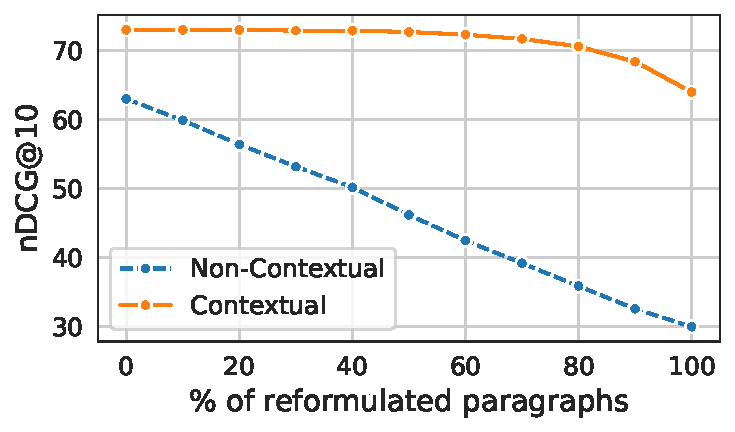
\includegraphics[width=0.65\textwidth]{images/conteb_images/reformulated.pdf}
    \caption[Importance of contextual information]{\textbf{Importance of Contextual Information:} Starting from a set of queries and mostly self-contained document paragraphs from the \emph{Football}, we progressively reformulate paragraphs to remove information redundant with the rest of the document. This leads to sharp performance declines in standard retrieval approaches, but not in contextual retrieval approaches.}
    \label{fig:reformulated}
\end{figure}

% In most applications, documents exhibit a highly structured format where individual paragraphs are not intended to be understood in isolation. Instead, they rely on prior context, document structure, or domain-specific knowledge. Acknowledging this is therefore necessary to incorporate all the relevant information into the representation of a passage.


\begin{figure*}[ht]
    \centering
    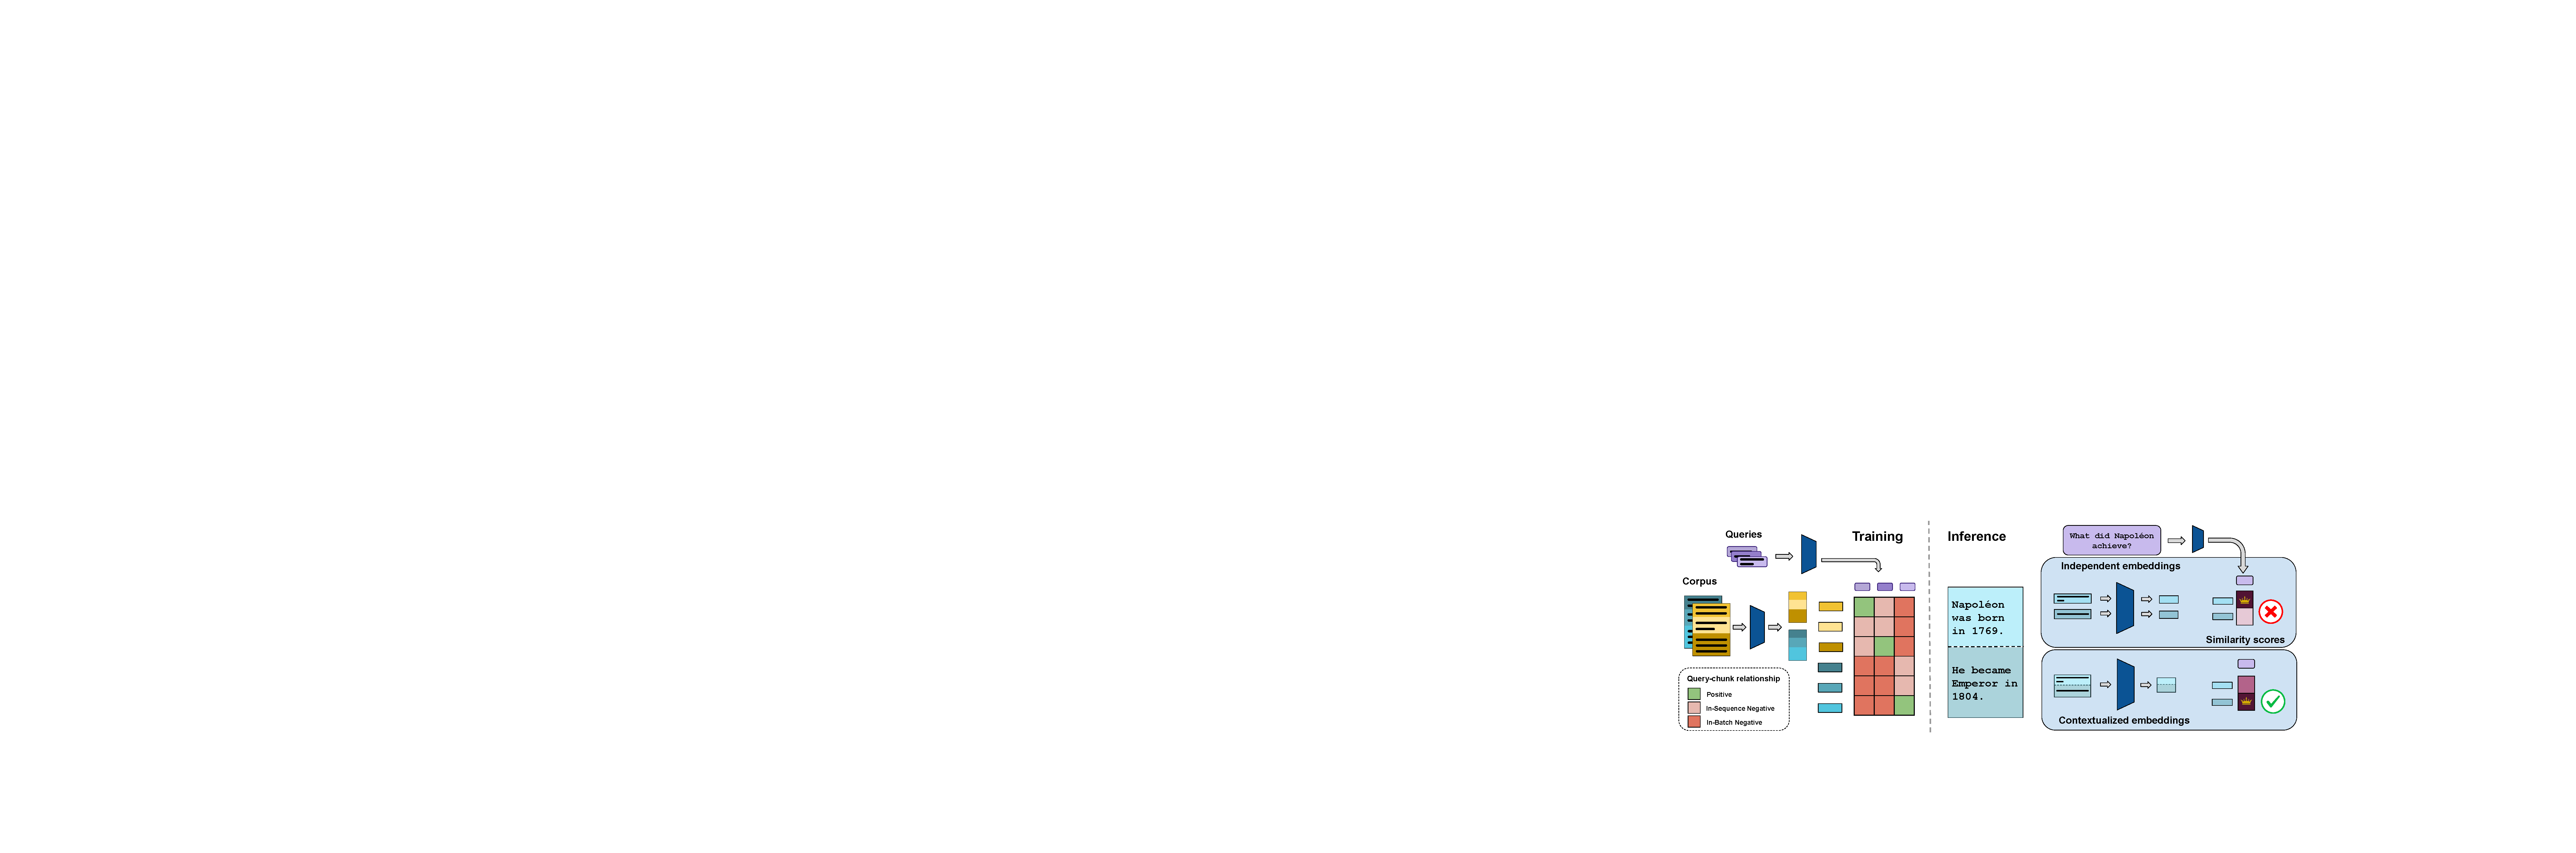
\includegraphics[width =\linewidth]{images/conteb_images/training_inference_final.pdf}
    \caption[Training vs inference overview]{
    \textit{Training (Left).} With respect to a single query, each chunk inside a batch plays a different role, depending on its original document, and the positive chunk.
    \textit{Inference (Right).} Traditional embedding methods (top) produce embeddings that do not include potentially essential contextual information. Contextualized embeddings (bottom) can integrate document-wide information in individual chunk representations, augmenting embedding relevance and improving downstream retrieval performance.}
    \label{fig:contextualized_exemple}
\end{figure*}

%\noindent\textbf{Industry Gap.} 
While long context encoders have been recently developed \sidecite{zhang2024mgte, modernbert, boizard2025eurobert} along with long context embedding models \sidecite{zhu2024longembedextendingembeddingmodels}, modern document retrieval pipelines typically segment lengthy documents into smaller chunks to optimize the granularity for efficient retrieval and readability of the retrieved content \sidecite{xu2024retrievalmeetslongcontext, jiang2024longragenhancingretrievalaugmentedgeneration}. Traditionally, these chunks are then \emph{independently} fed to an embedding model, and stored in a vector database for efficient future query matching. By doing so, these systems remove strong semantic and conceptual links between the split passages, directly affecting the resulting representations. An example is illustrated in \autoref{fig:contextualized_exemple}: embedding the sentence \textit{"He became emperor in 1804."} without leveraging information about the person at hand (\emph{Napoléon}) given in previous paragraphs will make matching queries related to \emph{Napoléon} difficult.

Recognizing the significant business value of incorporating broader contextual information into retrieval, major companies have explored leveraging large generative language models (LLMs) to mitigate this limitation. Some approaches attempt to circumvent retrieval altogether by feeding millions of tokens into the model's context window at runtime \sidecite{geminiteam2024gemini15unlockingmultimodal}, while others reformulate individual passages by concatenating them with document-level summaries and context \sidecite{contextual_anthropic}. However, these methods are prohibitively expensive at scale when dealing with corpora comprising thousands of documents.


%\noindent\textbf{Benchmarking.} 
Despite the critical importance of contextualized retrieval, standard benchmarks fail to capture this challenge. Evaluations traditionally focus on assessing the effectiveness of embedding models \sidecite{thakur_beir_2021, muennighoff_mteb_2022, saadfalcon2024benchmarkingbuildinglongcontextretrieval}, but they rely on datasets where document chunks are by design self-contained answer to the queries, which is a largely idealized scenario in practice \sidecite{thakur2025freshstackbuildingrealisticbenchmarks}. Consequently, benchmarks fail to highlight the limitations of current retrieval strategies in handling context-dependent passages. Worse, recent findings by \sidecite{zhou2025gsminfinitellmsbehaveinfinitely} indicate that some widely-used benchmarks exhibit biases that favor standard context-agnostic retrieval methods. Companies such as Anthropic have acknowledged these issues and maintain proprietary contextual retrieval benchmarks that remain unavailable to the public\sidenote{\url{https://www.anthropic.com/news/contextual-retrieval}}, underscoring the gap between academic evaluations and real-world industrial needs.

% To evaluate retrieval models, benchmarks such as BEIR \sidecite{thakur_beir_2021}, MTEB \sidecite{muennighoff_mteb_2022}, LoCo \sidecite{saadfalcon2024bencxhmarkingbuildinglongcontextretrieval} have been introduced, offering diverse real-world retrieval tasks. However, in practical settings, additional structural priors exist within the corpus providing information beyond mere document contents.


%
% Queries are generated for targeted passages, which results in scenarios where understanding the big picture of a document is unnecessary to correctly assign a chunk to its corresponding query. We aim at overcoming this pitfall by carefully crafting context-oriented evaluation samples.


% Other variant for the above sentence: Query-passage pairs are generated in such a way that understanding the big picture of a document is unnecessary to correctly assign a chunk to its corresponding query.
% While evaluations of document retrieval systems have traditionally focused on assessing embedding model quality \sidecite{thakur_beir_2021, muennighoff_mteb_2022}, they often neglect an important reality: document chunks are not independent - in practice, chunks most often originate from structured documents where information is naturally ordered and contextually linked. --> rephrased this
% Ignoring these relationships can lead to suboptimal retrieval performance, particularly when a chunk lacks sufficient context to be fully understood.

%In this work, we focus on evaluating retrieval systems on their capacity to efficiently leverage contextual information to construct meaningful chunk representations.

\noindent\textbf{Contribution 1: \textit{ConTEB}.}  
We introduce the \emph{Context-aware Text Embedding Benchmark}, designed to assess the ability of retrieval systems to leverage information from the entire document when indexing and retrieving document chunks. \emph{ConTEB} comprises both custom-designed tasks for fine-grained analysis, and practical retrieval evaluation settings spanning multiple document types, domains, and situations in which leveraging context is helpful to produce more meaningful chunk representations. 
We evaluate standard embedding methods on the benchmark and find they struggle when contextual awareness is required, while highlighting the promising contextual capabilities of approaches such as \emph{Late Chunking} \sidecite{LateChunking}.

\noindent\textbf{Contribution 2: \textit{Efficient Contextual Training}.}  
Improving upon the \textit{Late Chunking} method \sidecite{LateChunking}, we propose a novel embedding post-training method that optimizes information propagation between same-document chunks at indexing time to ensure embeddings are better contextualized. Our method largely boosts performance on \emph{ConTEB} %\textcolor{red}{over both non-contextual and training-free baselines, }
with minimal computational overhead. 
Through extensive ablations, we detail critical design choices and show our method displays increased robustness to sub-optimal chunking strategies and produces representations that scale better with corpus size. 

We open-source all project artifacts, including the benchmark, models and training data\sidenote{ \url{https://github.com/illuin-tech/contextual-embeddings}}.

% Document Retrieval consists in matching a user query to relevant documents in a given corpus. It is central to many industrial applications, either as a standalone ranking system (search engines) or as part of more complex information extraction or Retrieval Augmented Generation (RAG) pipelines. \manu{rephrase here, this is the colpali intro}

% \manu{briefly describe the process of indexing documents}
% Modern document retrieval pipelines often involve several phases; given a corpus of documents to index, a text extraction phase must first be conducted, in which documents will be parsed and chunked into a series of "chunks" of reduced length. These chunks are dimensioned to be short enough to XXX ([readable by a human, not exceeding context size, rag systems], yet they should ideally be of sufficient size to contain enough information to be somewhat self-contained thus providing  useful context to respond to a user's query.
% These chunks are then fed independently to text embedding models to obtain a vectorized chunk representation, which are stored in a vector database. Assessing the performance of document retrieval systems has historically most often been considered through the lens of embedding model evaluation. These evaluations are designed without consideration for the fact chunks are not independant and we may have priors on the corpus (such as the reading order in which to consider the chunks, the ones that come from the same document, their context, their amount, etc).

% In this paper, we focus on a main failcase of embedding models, which is when a chunk lacks sufficient conytext to be understood. 
% % cite the figure


% \begin{figure}
%     \centering
%     \includegraphics[width = 0.45\textwidth]{images/conteb_images/contextualized_example.png}
%     \caption{\manu{{Temporary placeholder figure}}}
    
%     % Latencies indicated in the figure are computed on the same machine \code{g2-standard-16} with a NVIDIA-L4 GPU, and averaged over 100 pages. Further details in \autoref{subsection:latency}.The computed score is the average of from all datasets in \textit{ViDoRe} for PDF Parser + Captioning and ColPali respectively. Further details in \autoref{section:results}.} 
%     \label{fig:contextualized_exemple}
% \end{figure}


% In this work, we focus on integrating contextual information into a given passage's latent representation.


% \noindent\textbf{Contribution 1: \textit{Context-aware embedding evaluation}.}
% We propose CAEEL, the Context-aware embedding evaluation Leaderboard, a series of retrieval-oriented tasks spanning multiple document types and domains \manu{and languages ?} that aims to assess the capacity of a retrieval system to leverage prior contextual information about passages in the construction of their embeddings. We show current top models struggle.

% \noindent\textbf{Contribution 2: \textit{In-sequence negative training strategy}.}
% Leveraging recent advances in long-context encoder models, and extending work on late chunking, we propose a novel modeling and training approach to seamlessly integrate context in passage representations with very little compute overhead. We show our approach, consisting of training with in-sequence negatives, is well aligned with standard retrieval applications and boosts performance. Our codebase which we openly release is model agnostic and is compatible with all sentence-transformers embedding models.



% \textbf{Contribution 4.}
% We release our fine-tuned models and training code under open licenses, bringing to both researchers and industry practitioners state-of-the-art document retrieval models\sidenote{\url{hf.co/anon}}. We also release all artifacts related to benchmarking\sidenote{\url{github.com/anon}} (data, evaluation code, public leaderboards, reproducible baselines) to serve as a new reference for Document Retrieval.



% \noindent\textbf{Problem Setting.}
% In our setting, a retrieval system scores how relevant a document $d$ from corpus 
% \manu{add math}

% Neural embedding models to represent texts at a passage level were introduced by \sidecite{reimers2019sbert} \manu{little history recap}. \manu{mention synthetic data, infonce, late interaction}. Long context models.

% To evaluate such models \manu{beir, mteb}.In practice, much more priors exist on the data distribution within the corpus. \manu{add math to show we have knowledge of D in its entirety often times, and metadata that enables us to have a stucture on D.} Long context evaluation.

% Modern  techniques have been developped to compensate for the incapacity of embedding models to integrate knowledge beyond their passage scope. \manu{mention smart chunking techniques + contextual embeddings antrhropic, raptor, graph rag}

% All these techniques however either necessitate heavy intervention of external LLMs (reformuation), are hard to scale to large corpora, or are very brittle and based on carefully crafted heuristics or document parsing approaches (chunking) which have been shown to be suboptimal [CITE].


% \noindent\textbf{Late Chunking.} Late chunking is a training-free pooling token pooling technique \manu{add math about late chunking} Authors have designed the method to be able to reduce the chunk size while maintaining strong performance. We are interested in seeing whether through training we can induce better information propagation and optimize the method...

\section{Problem Formulation \& Related Work}

% \subsection{Problem statement}
% As illustrated in \autoref{fig:contextualized_exemple}, embedding models that disregard document-level context often lack crucial information. In the example, the pronoun "They" refers to an entity mentioned earlier, which must be resolved to ensure correct chunk embeddings for queries about the Brazilian Football team. More broadly, retrieval systems integrate with document ingestion pipelines, leveraging metadata such as document membership and chunk position. This work explores utilizing these priors to enhance retrieval in context-dependent scenarios.

%M In standard retrieval pipelines, long documents are chunked and independently processed by an embedding model. 
% \pierre{embeddings that do not leverage contextual information from the chunking step will lack of essential information : ici je reciterais la figure 1 du dessus}

% \subsection{Contextual chunk representation}
% \manu{Probably remove this entire paragraph, or change with figure 2.} As illustrated in \autoref{fig:reformulated}, embedding models that do not consider document-level knowledge ("context") will often lack essential information when producing a chunk representation. In the illustration (\autoref{fig:contextualized_exemple}), the pronoun \textit{"They"} in the second chunk is ambiguous without context. Retrieval models that are able to leverage contextual information will have a much easier time matching this chunk to queries about either Brazilian football or Napoleon. Generally, it is straightforward to inject contextual information such as the source document, or the position of the chunk within it. Systematically incorporating these priors to improve retrieval is the focus of this work.

\subsection{Retrieval Frameworks}
In this paper, we consider the traditional retrieval framework where a retrieval system given a query \(q\), searches a corpus \(\mathcal{D}\) for relevant documents. Each document \(d \in \mathcal{D}\) is scored based on its content by first embedding the text into a vector space, and then computing a similarity measure. The similarity between a query \(q\) and a document \(d\) is defined as
\begin{equation}
\text{sim}(q, d) = f\big(\phi(q), \phi(d)\big) \nonumber
\end{equation}
where \(\phi\) maps text into an \(n\)-dimensional vector space and \(f: \mathbb{R}^n \times \mathbb{R}^n \to \mathbb{R}\) is a similarity function, such as cosine similarity or dot product.

In applied settings, individual documents are often too long to be practical for retrieval purposes \sidecite{Liu_LlamaIndex_2022, mixofgranularity}. % \manu{expand and illustrate}
Each document \(d\) is thus divided into segments called \emph{chunks} by a partitioning function \(\mathcal{P}\) defined as
\begin{equation}
\mathcal{P}(d) = \{c_1, c_2, \dots, c_{N_d}\} \nonumber%, d = \bigcup_{i=1}^n c_i \nonumber
\end{equation}


% with each chunk \(c_i\) representing a segment of \(d\) and $N_d$ represents the number of chunks in the document $d$.

% The complete set of metadata across the corpus is given by
% \[
% M = \{M_c \mid c \in \mathcal{D}\}.
% \]
% The retrieval function \(\text{sim}(q, c)\) assigns a relevance score to a query \(q\) and a chunk \(c\). 
In the \emph{standard retrieval} setting, the score is computed solely based on chunk content:

\begin{equation}
\text{sim}(q, c) = f\big(\phi(q), \phi(c)\big) \nonumber
\end{equation}

 Additional information (priors) is however often available to the document embedding system. Typically, knowledge of the entire corpus $\mathcal{D}$, or of \emph{structural metadata} \(M_c\) such as neighboring document chunks obtained through \(\mathcal{P}\), can be leveraged by a modified embedding function \(\phi_2\), yielding the following similarity score:
\begin{equation}
\text{sim}(q, c) = f\Big(\phi(q), \phi_2\big(c, M_c, \mathcal{D}\big)\Big) \nonumber
\end{equation} 

\noindent\textit{This work is centered on efficiently integrating priors about the entire document when embedding a sub-document chunk.}


% \noindent\textbf{Problem Setting.} In our setting, a retrieval system assigns a relevance score to a document $d$ from a corpus $\mathcal{D}$ given a query $q$. Typically, this involves computing a similarity function $\text{sim}(q, d)$ using dense or sparse representations:
% \begin{equation}
% \text{sim}(q, d) = f(\phi(q), \phi(d))
% \end{equation}
% where $\phi$ is an embedding function that maps text into a vector space, and $f$ measures similarity, commonly using cosine similarity or dot product.

% Let $\mathcal{D}$ denote a corpus composed of multiple documents $d \in \mathcal{D}$, where each document $d$ is further composed of multiple chunks $c \in d$. The chunking process is defined by a partition function $\mathcal{P}$ such that:
% \begin{equation}
%     \mathcal{P}: d \to \{c_1, c_2, \dots, c_n\}, \quad \forall d \in \mathcal{D}, \quad c_i \in d.
% \end{equation}

% As the retrieval system itself often handles this decomposition,  the additional structural priors, including the fact that chunks originate from the same document and their relative positions within that document are known and usable by the system during indexing. We denote this metadata information by $M = \{M_c \mid c \in \mathcal{D}\}$, where $M_c$ includes document membership and ordering constraints.

% The retrieval function $S(q, c)$, which assigns a relevance score to a query $q$ and a chunk $c$, can be defined in two settings:

% \noindent\textbf{Standardly}: The retrieval model assigns a score based purely on content similarity:
%    \begin{equation}
%        \text{sim}(q, c) = f(\phi(q), \phi(c))
%    \end{equation}
%    where $f(q, c)$ is a function of the semantic similarity between the query and the chunk, typically computed via dense embeddings or lexical matching.

% \noindent\textbf{With Structural Priors}: The scoring function incorporates metadata $M_c$, allowing it to leverage document structure:
%    \begin{equation}
%        S(q, c) = f(\phi(q), \phi_2(c, M_c, \mathcal{D})
%    \end{equation}
%    where $M_c$ contains structural priors such as inter-chunk relationships, document cohesion, and positional significance.


\subsection{Integrating Contextual Information} \label{related_work_contextual}
Neural embedding models for passage-level text representation, popularized by SentenceBERT \sidecite{reimers2019sbert}, have enabled retrieval systems to move beyond lexical matching \sidecite{robertson_okapi_1994}. To include contextual information in these retrievers, previous works proposed methods that either operate \textit{offline} during \emph{indexing}, or online during \emph{querying} when faced with a user request.

\noindent\textbf{Indexing.} The chunking strategy is a crucial design choice and often aims to optimize chunk self-containment. Fixed-size approaches with overlaps preserve continuity, while structure-aware chunking respects natural text boundaries, such as paragraphs or sentences. Semantic chunking, by contrast, splits text into topic-aligned segments. These methods appear in frameworks such as LlamaIndex \sidecite{Liu_LlamaIndex_2022} and LangChain \sidecite{chase_langchain_2022}, but different queries may need different chunk sizes. Thus, dynamic chunking techniques have emerged to adapt segmentation on the fly \sidecite{mixofgranularity, qian2024groundinglanguagemodelchunkingfree}. Beyond optimizing chunking, some indexing approaches enrich chunks with broader context by preprending LLM-generated document summaries, contextual information or metadata \sidecite{contextual_anthropic, multimetarag}. Similarly, \sidecite{morris2024contextualdocumentembeddings} demonstrate that appending learned "corpus" embeddings to queries and documents can further improve retrieval. Other indexing-time techniques involve organizing chunks into higher-level data structures. For example, \sidecite{graphrag} and \sidecite{raptor} cluster related chunks into semantic graphs or tree hierarchies.

%\textcolor{red}{\sidecite{LateChunking} introduced the \textit{Late Chunking} paradigm, which leverages the large context window of embedding models to enable cross-chunk information propagation, yielding small improvement gains on standard retrieval datasets, hinting at chunk contextualization potential.}

\noindent\textbf{Querying.} In contrast, \emph{query-time} solutions rely on iterative or agentic loops to refine retrieval dynamically. LLMs can be used to iteratively update the query or request additional chunks based on partial results \sidecite{MultiHopRAG, IrCoTRAG}, or even to run “self-checks” and seek extra context when needed \sidecite{selfrag}. While these adaptive techniques can better address complex, multi-hop queries, they typically require much more computational resources during inference.

% \manu{rewrite} In this paper we propose a method to efficiently leverage document-level contextual information during indexing without the need for external LLMs and with no computational overhead.


%\subsection{Integrating contextual information}



% \manu{here restructure}
% Neural embedding models for passage-level text representation were popularized with SentenceBert \sidecite{reimers2019sbert}, enabling semantic search beyond traditional lexical matching \sidecite{robertson_okapi_1994} have been widely adopted to train embedding models in retrieval tasks. 

% \subsection{Integrating contextual information.}
% \label{related_work_contextual}


% \manu{Restructure as indexing vs querying time approaches}

%The document partitioning process \(\mathcal{P}\) is crucial in optimizing the performance of retrieval systems. Chunks must strike a balance between two competing constraints: \textit{compactness} and \textit{self-containment}. They should be short enough to remain readable and fit within the context window of modern language models, but each chunk should also include enough contextual information to be interpretable on its own, reducing reliance on other parts of the document.

%Refining chunks to get the most suitable representations
% Building a context-aware retrieval system is a complex problem that can be tackled at different levels. Some solutions are implemented offline at document ingestion and indexing time,
%- refining chunks to get the most suitable representations - 
% while others trade inference time with elaborate retrieving algorithms to make sure that the relevant chunks can be found.

%\manu{simplify, add citations}
% \noindent\textbf{Optimizing Chunking.} 
% Effective chunking strategies are essential for optimal performance in language models. Commonly adopted approaches include structure-aware chunking, attempting to keep paragraphs and sentences together, and semantic chunking, splitting text based on meaningful units with similar topics. These techniques are found in the popular and widely used implementation frameworks \sidecite{Liu_LlamaIndex_2022, chase_langchain_2022}.
%Common approaches include fixed-size chunking, where text is divided into uniform segments with possible overlaps to maintain context continuity, Structure-Aware chunking where chunks attempts to keep paragraphs and sentences together, and semantic chunking, splitting text based on meaningful units with similar topics. All of these techniques are found in the popular and widely used implementation frameworks \sidecite{Liu_LlamaIndex_2022, chase_langchain_2022}.
%, ensuring each chunk conveys a complete idea
% However, there is no one-size-fits-all solution since the optimal granularity of the chunk depends directly on the query at hand, which motivated dynamic chunking methods \sidecite{mixofgranularity, qian2024groundinglanguagemodelchunkingfree}.
% Hybrid chunking combines both methods, adjusting chunk sizes dynamically to balance readability and context preservation. These strategies aim to create chunks that are both manageable for processing and rich in information, facilitating more accurate and efficient retrieval. --> maybe no need to expand on hybrid approaches as we don't have specific examples to cite

% \noindent\textbf{Context Infusion.} Some approaches leverage the long-context capabilities of LLMs to refine chunks by incorporating broader context in the form of concatenated text \sidecite{contextual_anthropic} and metadata \sidecite{multimetarag}, leading to improved retrieval performance at higher corpus ingestion costs. Concatenating corpus-level vector representations to queries and documents before feeding them to an embedding model \sidecite{morris2024contextualdocumentembeddings} has also been shown to yield performance improvements. 

%Enhancing chunk representations can be achieved by employing large language models (LLMs) that access document-wide information. By incorporating broader context in the form of concatenated text \sidecite{contextual_anthropic} and metadata \sidecite{multimetarag}, these approaches leverage the long-context capabilities of LLMs to generate more accurate and relevant representations of chunks, leading to improved retrieval performance at higher corpus ingestion costs. Techniques such as concatenating corpus-level representations to query and document token embeddings \sidecite{morris2024contextualdocumentembeddings} have also been shown to yield performance improvements.

% (reformulated above) This approach, known as contextual retrieval, utilizes techniques like contextual embeddings and contextual BM25 to improve the retrieval step in retrieval-augmented generation (RAG) systems. By incorporating broader context, LLMs can generate more accurate and relevant representations of chunks, leading to improved retrieval performance. 

% \noindent\textbf{Structured Corpus Representation.} Organizing documents into a data structure is yet another approach that aims at improving retrieval. At ingestion time, chunks can be assembled into structures such as graphs \sidecite{graphrag} or trees \sidecite{raptor} based on their semantic similarity, often with the help of LLMs. These methods leverage the structured relationships between entities to provide more comprehensive and contextually relevant information during retrieval.
%, enhancing the overall performance of the system. 

%\noindent\textbf{Graph-Enhanced Retrieval.} Incorporating document relationships, such as citation graphs, into retrieval processes can significantly improve quality. GraphRAG, for instance, integrates knowledge graphs and graph databases with traditional retrieval-augmented generation techniques. This method leverages the structured relationships between entities to provide more comprehensive and contextually relevant information during retrieval, enhancing the overall performance of the system. 

% \noindent\textbf{Inference-Time Approaches.} LLMs can be used in agentic loops to iteratively refine queries and improve retrieval quality. Complex pipelines \sidecite{selfrag, MultiHopRAG, IrCoTRAG} involve the LLM over multiple steps, evaluating iteratively whether additional chunks should be retrieved. 

% \noindent\textbf{Inference-Time Approaches.} LLMs can be used in agentic loops to iteratively refine queries and improve retrieval quality. \sidecite{selfrag} employs the generations to trigger and evaluate the retrieval mechanism, while SeaKR \sidecite{SeaKR} does so using the LLM internal states. Multi-hop approaches \sidecite{MultiHopRAG, IrCoTRAG} involve the LLM over multiple steps, evaluating iteratively whether additional chunks should be retrieved. 
% At inference time, advanced strategies like self-retrieval augmented generation (Self-RAG) and multi-hop retrieval are employed to enhance performance. Self-RAG involves the model retrieving and utilizing its own generated content to refine answers, while multi-hop retrieval allows the model to gather information from multiple related documents or chunks to answer complex queries. These methods aim to reduce computational overhead and improve scalability by minimizing reliance on external interventions and heuristics.

% Despite their success, these methods often rely on computationally expensive LLMs either during indexing or querying, and are impractical to scale to larger corpora.
% \manu{mention late chunking}


\section{\textit{ConTEB}: Context-aware Text Embedding Benchmark}


% \section{\textit{ConTEB}: Context-Aware Embedding Leaderboard}
\label{section:loco_benchmark}

% \manu{This section needs to highlight the fact that existing datasets are not adapted, nor easily adaptable for our tasks. There is a real "extractive" bias in existing datasets which causes questions to be super extractive and often self contained.}




\begin{comment}
\begin{table*}[h]
    \centering
    \scriptsize
\resizebox{\linewidth}{!}{
    \begin{tabular}{lcc|cc}
    \toprule
     & Chunk Annotation & Verification & Domain & Context requirement type \\
    \midrule
    \vspace{1mm}\textbf{In Domain} & \\
    MLDR & Synthetic & & Encyclopedic & Document-level reasoning \\
    NarrativeQA & Synthetic & & Literature & Document-level reasoning \\
    SQuAD & Manual & & Encyclopedic & Chunk not self-contained  \\
    \midrule
    \vspace{1mm}\textbf{Out-Of-Domain} & \\
    Footballers & By design & \darkgreencheck  & Sports & Co-reference resolution \\
    Geography & By design & \darkgreencheck & Geography & Co-reference resolution \\
    Insurance & By design & \darkgreencheck & Insurance & Structure understanding \\
    Covid-QA & Synthetic & & Medical & Chunk not self-contained \\
    ESG Reports & Manual & & Industry  & Context disambiguation \\
    NanoBEIR* & Manual & & Varied & - \\
    \bottomrule
    \end{tabular}
    }
  \captionof{table}{ConTEB details}
  \label{tab:conteb_details}
\end{table*}
\end{comment}


\begin{comment}
\begin{table}
    \centering
    \scriptsize
    \resizebox{\linewidth}{!}{%
    \begin{tabular}{lcccc}
    \toprule
     & Pairing & Verification  \\
    \midrule
    \vspace{1mm}\textbf{In Domain} & \\
    MLDR & Synthetic &  & \\
    NarrativeQA & Synthetic &  \\
    SQuAD & Existing &  \\
    \midrule
    \vspace{1mm}\textbf{Out-Of-Domain} & \\
    Footballers & By design & \darkgreencheck \\
    Geography & By design & \darkgreencheck \\
    Insurance & By design & \darkgreencheck \\
    Covid-QA & Synthetic &  \\
    ESG Reports & Manual &  \\
    NanoBEIR* & Existing &  \\
    \bottomrule
    \end{tabular}
    }
    \label{tab:example}
    \captionof{table}{Example table}
\end{table}
\end{comment}


% LaTeX code for a compact ConTEB statistics table (no zebra striping)
% Required packages (add to your preamble if not already present):
%   \usepackage{booktabs, siunitx, xcolor, colortbl, multirow, graphicx, array}
%   \sisetup{detect-all}

\begin{table*}[ht]
  \centering
  \small

  % ------- siunitx column configuration (slightly narrower) -------
  \sisetup{
    table-number-alignment = center,
    table-figures-integer  = 4,
    table-figures-decimal  = 1,
    table-column-width     = 12mm,
  }

  % ------- custom colors for group labels -------
  \definecolor{grpA}{HTML}{C6E0FF}   % In-Domain background
  \definecolor{grpB}{HTML}{FFD6D6}   % Out-of-Domain background

  % ------- helper for fixed-width first column (vertical labels) -------
  \newcolumntype{C}[1]{>{\centering\arraybackslash}p{#1}}

  % ------- slightly larger rows to fit sentences -------
  \renewcommand{\arraystretch}{1.25}

  \begin{tabular}{
      C{5mm}                          % Domain group (fixed width, centered)
      l                                % Dataset name
      S[table-format=3.1]                % # Queries
      S[table-format=3.1]                % # Docs
      S[table-format=3.1]              % Tokens / Chunk
      S[table-format=3.1]              % Chunks / Doc
      c
      % p{40mm}                          % 5-word sentence (fixed width)
  }
  \toprule
   & Dataset & {Queries} & {Docs} & {\shortstack{Tokens per\\[-1pt]Chunk}} & {\shortstack{Chunks per\\[-1pt]Document}}  & {Context Utilization} \\
  \midrule
  % ---------------- In-Domain ----------------
  \multirow{3}{*}{{\rotatebox[origin=c]{90}{\shortstack{\textbf{In}\\[-1pt]\textbf{Domain}}}}}
    & MLDR      &  100 &  100 & 170.5 & 15.4 & Document-level reasoning \\
    & NarrativeQA       & 8575 &  355 & 154.5 &  4.9 & Document-level reasoning   \\
    & SQuAD     & 2067 & 2067 &  19.1 &  8.5 & Chunk not self-contained \\
  \midrule
  % -------------- Out-of-Domain --------------
  \multirow{6}{*}{{\rotatebox[origin=c]{90}{\shortstack{\textbf{Out of}\\[-1pt]\textbf{Domain}}}}}
    & {\color{navyblue}\textbf{Football}}   & 2682 & 301 &  77.4 &  20.8 & Co-reference resolution \\
    & {\color{navyblue}\textbf{Geography}}  & 5283 &  530 & 113.6 &  4.3 & Co-reference resolution     \\
    & {\color{navyblue}\textbf{Insurance}}  &  120 &    1 &  80.7 & 60.0 & Structure understanding \\
    & Covid-QA            & 1111 &  115 & 153.9 & 29.1 & Chunk not self-contained  \\
    & ESG Reports         &   36 & 30 & 205.5 & 123.4 & Context disambiguation \\
    & NanoBEIR$^*$        &  650 & 56723 & 199.4 &  1 & No context is needed  \\
  \bottomrule
  \end{tabular}

  \caption[ConTEB dataset details]{Merged \emph{ConTEB} dataset details. Controlled datasets are highlighted in {\color{navyblue}\textbf{bold blue}}. NanoBEIR values are summed over the 13 datasets that compose it.}
  \label{table:merged_conteb}
\end{table*}

%      & Chunk Annotation & Verification & Domain & Context requirement type \\
%     \midrule
%     \vspace{1mm}\textbf{In Domain} & \\
%     MLDR & Synthetic & & Encyclopedic & Document-level reasoning \\
%     NarrativeQA & Synthetic & & Literature & Document-level reasoning \\
%     SQuAD & Manual & & Encyclopedic & Chunk not self-contained  \\
%     \midrule
%     \vspace{1mm}\textbf{Out-Of-Domain} & \\
%     Footballers & By design & \darkgreencheck  & Sports & Co-reference resolution \\
%     Geography & By design & \darkgreencheck & Geography & Co-reference resolution \\
%     Insurance & By design & \darkgreencheck & Insurance & Structure understanding \\
%     Covid-QA & Synthetic & & Medical & Chunk not self-contained \\
%     ESG Reports & Manual & & Industry  & Context disambiguation \\
%     NanoBEIR* & Manual & & Varied & - \\
%     \bottomrule
%     \end{tabular}
%     }
%   \captionof{table}{ConTEB details}
%   \label{tab:conteb_details}
% \end{table*}


\subsection{Benchmark Design}

Existing benchmarks often rely on (or assume) self-contained document chunks. This creates a misleading perception that contextualization offers little to no benefit, which in practice is rarely the case. To address this gap, the \emph{ConTEB} benchmark philosophy is to explicitly be composed of tasks in which leveraging document-wide context should lead to performance improvements. Our benchmark originates from two sources: new datasets specifically created for \emph{ConTEB}, and repurposed academic datasets. We take special care in selecting data sources spanning from multiple domains, including realistic industrial scenarios.

\noindent\textbf{Why Context?} Context can help resolve ambiguity, such as distinguishing between multiple meanings of a word or resolving pronouns and entity references (co-reference resolution). It is crucial when documents have a structured format, like legal or scientific texts, where understanding table of content hierarchy is key to aid intra-document disambiguation. Inversely, document-level contextual information is key when querying a corpus of documents that follow a strongly similar structure, such as annual company reports, to enable cross-document disambiguation.

% We mix both tasks designed specifically to elicit context, and existing academic datasets repurposed for \emph{ConTEB}. Furthermore, we take special care in selecting data sources spanning from multiple domains, including realistic industrial scenarios.

% In our benchmark, retrieval performance is measured in scenarios where naive chunk-based approaches fail. By evaluating systems under these structured conditions, we provide a clearer picture of how well retrieval systems leverage context, rather than merely optimizing for chunk-level similarity.



% This enables the benchmark to cover an array of situations.
% \begin{table}[h]
%     \centering
%     \scriptsize
% \resizebox{\linewidth}{!}{
%     \begin{tabular}{lcc}
%     \toprule
%      & Domain & Context requirement type \\
%     \midrule
%     \vspace{1mm}\textbf{In Domain} & \\
%     MLDR & Encyclopedic & Document-level reasoning \\
%     NarrativeQA & Literature & Document-level reasoning \\
%     SQuAD & Encyclopedic & Chunk not self-contained  \\
%     \midrule
%     \vspace{1mm}\textbf{Out-Of-Domain} & \\
%     \textcolor{navyblue}{\textbf{Sports}} & Sports & Co-reference resolution \\
%     \textcolor{navyblue}{\textbf{Geography}} & Geography & Co-reference resolution \\
%     \textcolor{navyblue}{\textbf{Insurance}} & Insurance & Structure understanding \\
%     Covid-QA & Medical & Chunk not self-contained \\
%     Vidore-ESG Reports& Industry  & Context disambiguation \\
%     \bottomrule
%     \end{tabular}
%     }
%   \captionof{table}{\emph{ConTEB} constitution details. Controlled datasets are highlighted in \textcolor{navyblue}{\textbf{bold blue}}. The other datasets are stemming from academic benchmarks and repurposed for \emph{ConTEB}.}
%   \label{table:conteb_details}
% \end{table}

% \subsection{Benchmark Construction}
% \label{sec:bench-construction}

\noindent\textbf{Concept.} To isolate the importance of contextual cues and diminish other confounding factors, we construct three benchmark tasks to study contextualization in controlled experimental settings \sidecite{AllenZhu-icml2024-tutorial}. 
% By design, we ensure leveraging context is useful for these tasks. 
We also evaluate more practical retrieval settings at larger scale where we suspect contextualization to help, and in which we rely on organic, pre-existing query-document pairs.

\subsection{Benchmark Construction} 
%\begin{comment}
\begin{figure*}[htbp]
  \centering
  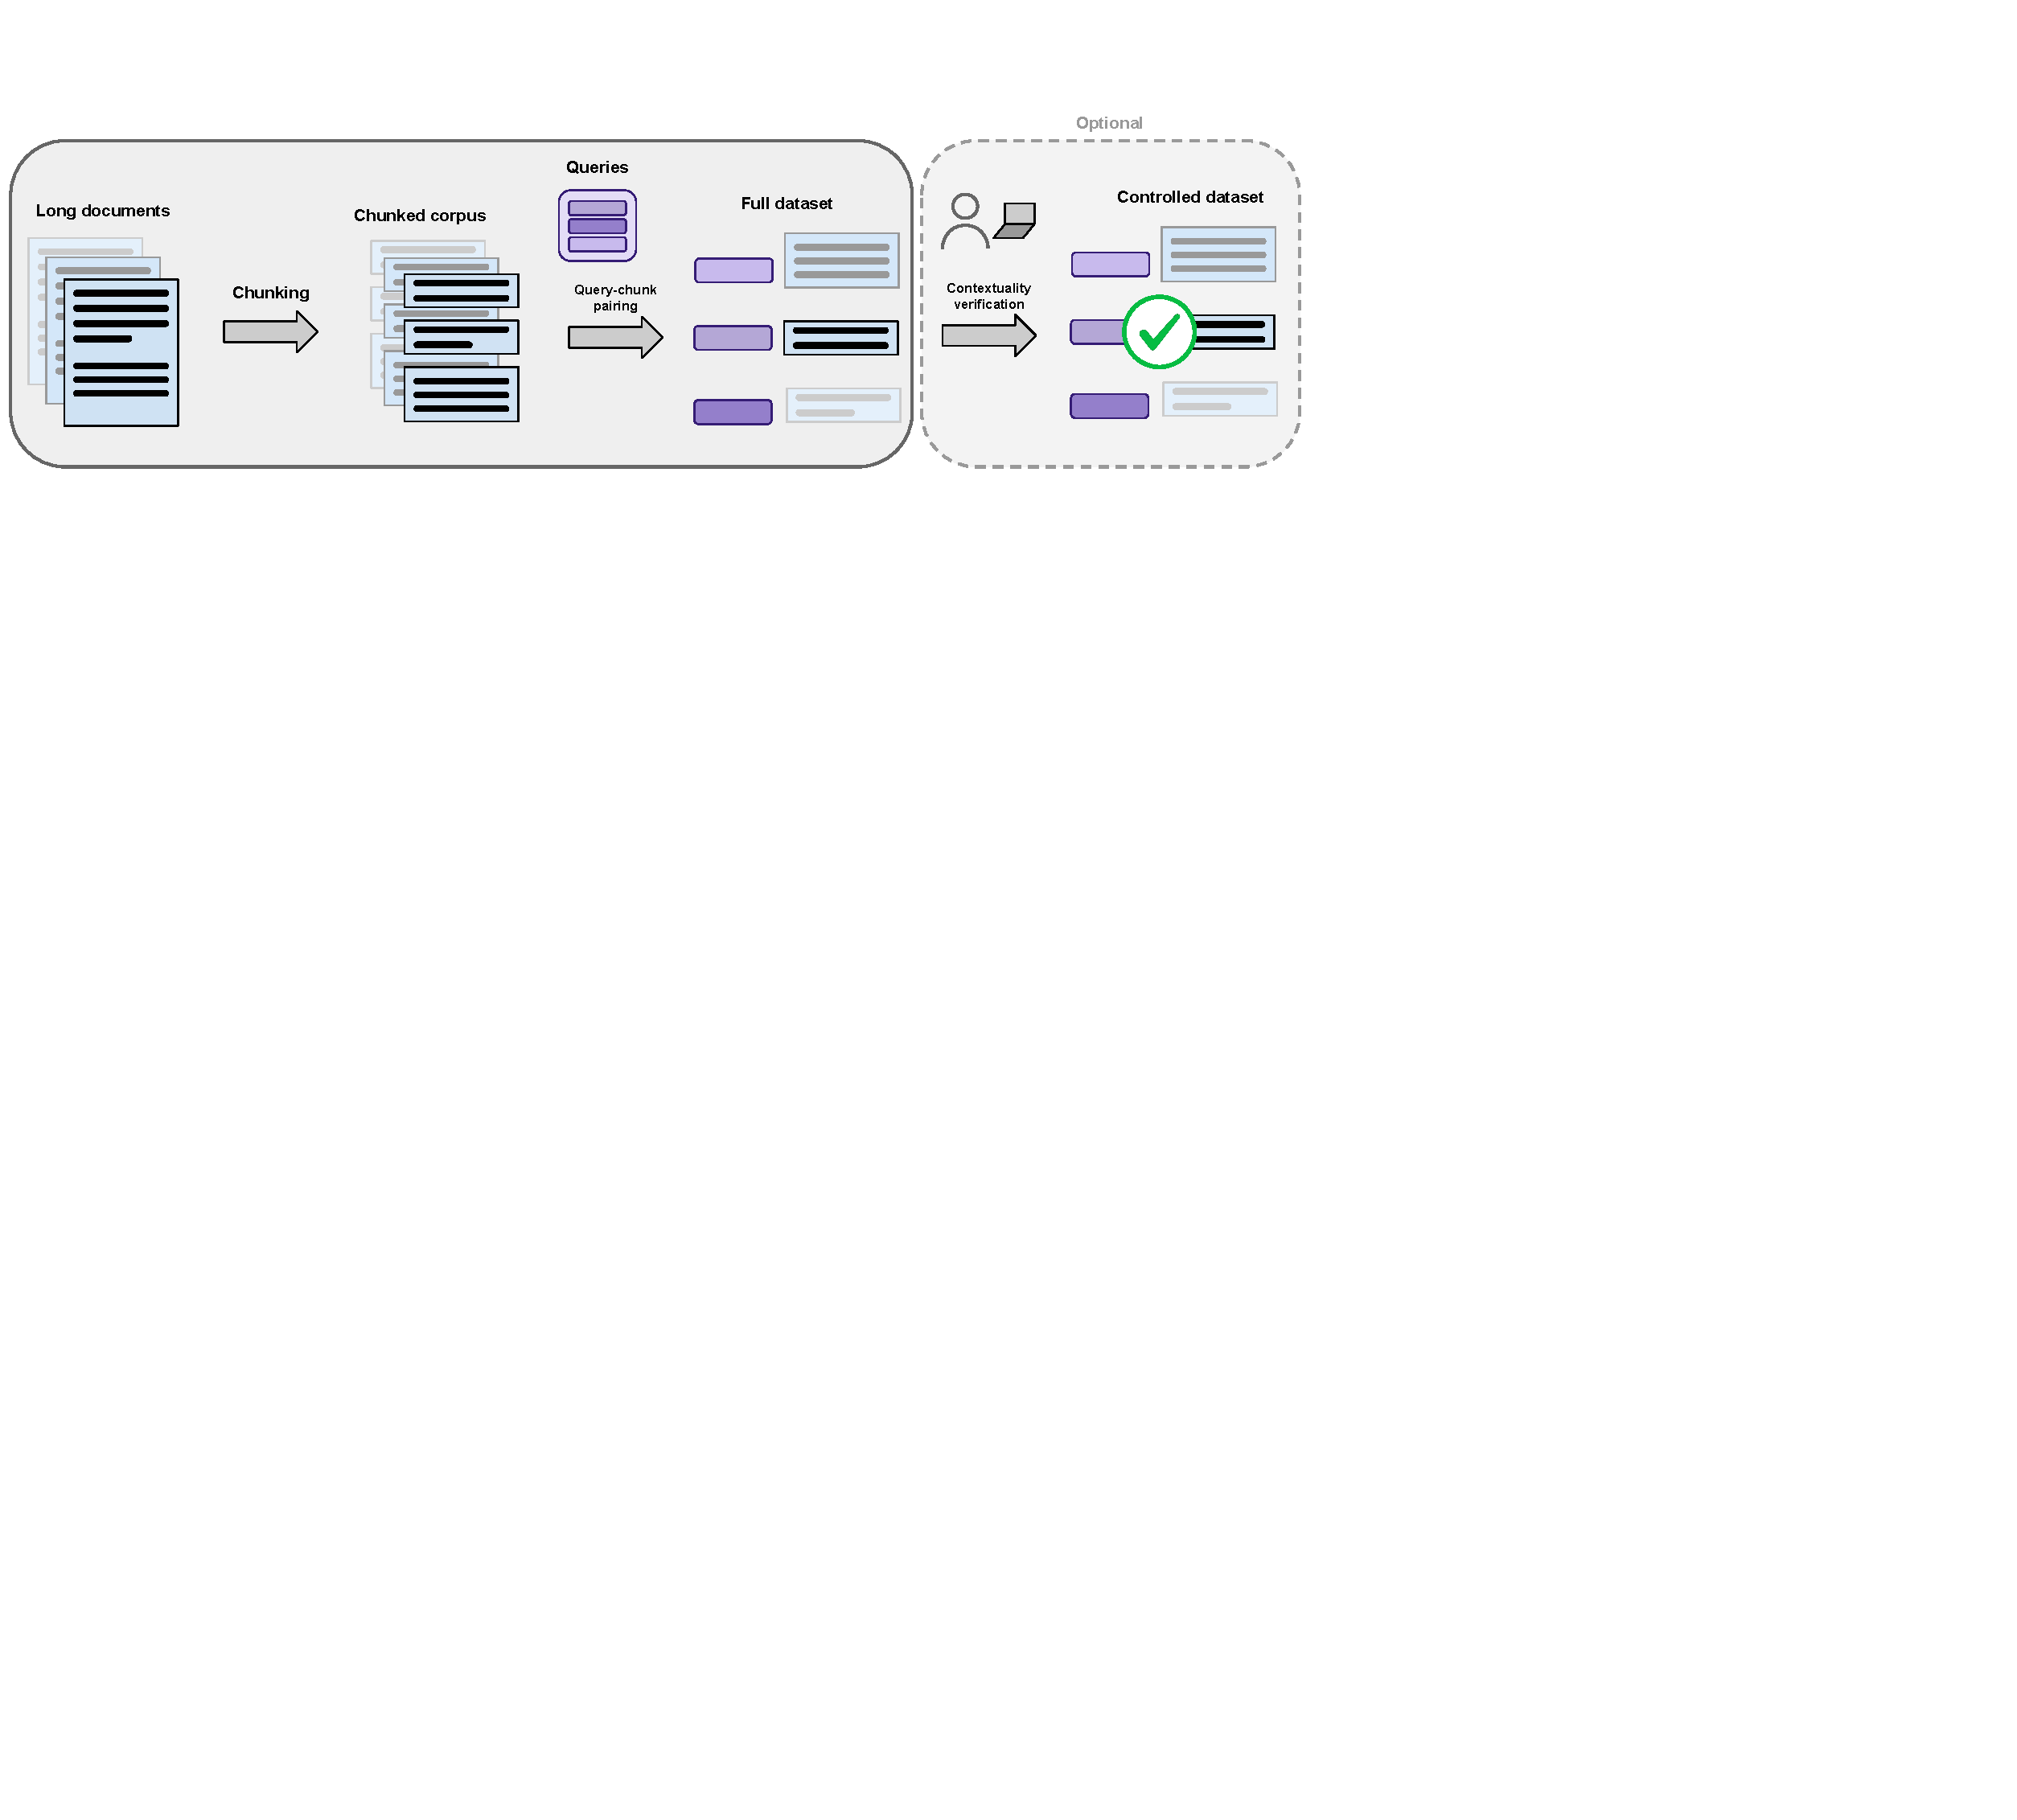
\includegraphics[width=1.3\textwidth]{images/conteb_images/benchmark_creation_horizontal.pdf}
  \caption[Benchmark creation process]{Benchmark creation process.}
  \label{fig:benchmark_creation}
\end{figure*}

% \textcolor{red}{ADD RELEVANT DETAILS FROM APPENDIX}
% Our generic benchmark curation pipeline is composed of three stages. 
% \textcolor{red}{Depending on the existing data at hand, each stage is applied slightly differently across all datasets.}
% We provide additional curation details in \autoref{app:conteb_stats}. 
% \textcolor{red}{
The generic dataset curation pipeline is depicted in \autoref{fig:benchmark_creation}. This three-stage process allows us to obtain queries linked to chunks belonging to long documents, that contain context with respects to each chunk. We apply this pipeline to each of our data sources, with minor adjustments depending on the existing data at hand, that we detail in \autoref{app:conteb_stats}. 
%In particular, we apply the optional stage of the pipeline to create our controlled setup.}

\noindent\textbf{1: Chunking.} We select long documents spanning a variety of domains and chunk them through a structure-aware method\sidenote{RecursiveCharacterSplitter with a threshold of 1000 characters \cite{chase_langchain_2022}} \sidecite{rajpurkar-etal-2016-squad, moller-etal-2020-covid, kočiský2017narrativeqareadingcomprehensionchallenge, chen_bge_2024, macé2025vidorebenchmarkv2raising}.

\noindent\textbf{2: Pairing.} 
%For datasets for which queries related to the longer original document are available, we associate them to the most relevant chunk(s) using existing manual annotations (SQuAD, ESG), or a large language model (CovidQA, MLDR, NarrativeQA). 
We use manual answer span annotations (\emph{SQuAD}, \emph{ESG}) or synthetically label them with a LLM (\emph{CovidQA}, \emph{MLDR}, \emph{NarrativeQA}), to match queries with chunks obtained in Stage 1. This ensures queries are not solvable by design \sidecite{thakur2025freshstackbuildingrealisticbenchmarks}. Alternatively, in our controlled experiment tasks, we generate queries pertaining to the chunks manually (\emph{Insurance}) or synthetically using LLMs (\emph{Football}, \emph{Geography}).


\noindent\textbf{3: Manual Verification \& Modification.}
%Sabotage.
The manually crafted questions in \emph{Insurance} are designed to be ambiguous without prior knowledge of the document structure. This is manually verified in this phase. Going a step further, in \emph{Football} and \emph{Geography}, we reformulate chunks with the help of a LLM to remove explicit mentions of the original document's theme which all queries mention. We do so in all but the first chunks of each document, explicitly enforcing the need for context.

In addition to our contextual scenarios, we use \emph{NanoBEIR} \sidecite{thakur_beir_2021} to evaluate non-regression on standard non-contextualized embedding tasks.

% We apply the optional control stage of the pipeline to three datasets--\emph{Footballers}, \emph{Geography}, and \emph{Insurance}--in order to enforce inter-chunk contextual links, to extensively test the capabilities of contextualization methods. The other datasets are adopted academic datasets, that we repurpose to our task with our pipeline, thereby introducing contextualization challenges. 
% Table \ref{table:conteb_details} provides an overview of the covered domains and the context types across datasets.
%\end{comment}

\noindent\textit{By combining hard tasks in controlled environments, repurposed academic benchmarks, and real-world industrial queries, our benchmark provides a comprehensive assessment of retrieval models in both standard and context-dependent retrieval scenarios.}

\subsection{Training Dataset}

Open training data is a key factor to ensure fair comparison across methods and robust conclusion. In addition to our benchmark, we construct and release a training dataset composed of query and document chunk pairs. It includes the training splits of \emph{MLDR} and \emph{NarrativeQA}, repurposed with our previously detailed pipeline. To increase the number of queries, we further use \emph{GPT-4o} to generate relevant supplementary synthetic queries. We also concatenate \emph{SQuAD} chunks from the same Wikipedia article, keeping track of the original question-passage associations. 
The full dataset contains 9881 unique long documents (3698 tokens on average), corresponding to a total of 232'587 chunks and 307'241 queries (see \autoref{app:training_data}). Scaling the dataset to more sources, through diverse synthetic augmentations and refinement–based augmentation methods \sidecite{lee2024nvembedimprovedtechniquestraining, wang2024improvingtextembeddingslarge} is left for future work.


\subsection{Baselines}
% In addition to raptor, cde, contextual, 0-shot sentence transformers, we train sentence transformers with the same data (same batch) than whazt we train CDE on.

%\pc{Pour moi faut se positionner et dire pourquoi on pool au niveau de la sentnece.} More recently, approaches such as late interaction models \sidecite{khattab2020colbert, chen_bge_2024} and  gained in popularity, setting new performance standards for encoder-based models. \pc{cokokok}


\noindent\textbf{Training-Free.} We evaluate a selection of off-the-shelf methods that are strong in their size categories such as a standard single-vector embedding model based on ModernBERT (\texttt{modernbert-embed-large} \cite{modernbert, ModernBERT-embed-large}), its multi-vector ColBERT equivalent \sidecite{khattab2020colbert, GTE-ModernColBERT} and \emph{Okapi BM25} \sidecite{robertson_okapi_1994}, a strong lexical matching method. 
Additionally, we compare against various contextualization approaches. Specifically, we include Anthropic’s contextual retrieval approach~\sidecite{contextual_anthropic}\sidenote{We use \texttt{Qwen-2.5-7B-Instruct} as the generative model which we serve on a 80GB A100 GPU with vLLM and \texttt{modernbert-embed-large} as the embedding model}, and evaluate Late Chunking \sidecite{LateChunking} without specific fine-tuning using \texttt{modernbert-embed-large}. These methods cover standard practices with varying level of complexities and indexing budgets.\sidenote{We also evaluate RAPTOR \cite{raptor} with \texttt{Qwen-2.5-7B-Instruct} and \texttt{cde-small-v2}~\cite{morris2024contextualdocumentembeddings} but find them to be poorly adapted to our problem settings.}

\noindent\textbf{Training-Based.} For fair evaluation, we also fine-tune the sentence embedding method \texttt{modernbert-embed-large} on the training dataset with the same batch construction strategy as when training our main method, ensuring performance differences only stem from methodological design.

% Our baselines are separated into two main categories: different training methods applied to the same base models that we use, and different embedding contextualization approaches.

% \noindent\textbf{ModernBERT-based baselines}
% We evaluate 4 different settings for the same base model: the base model itself, a version fine-tuned on our training dataset but in a single-context manner, a version applying late chunking without training, and our full version ContextEmbed \maxou{find name}.

% \noindent\textbf{Different embedding techniques}
% We compare our models to a sample of the different contextualization approaches detailed in \ref{related_work_contextual}, including Anthropic's contextual retrieval \sidecite{contextual_anthropic} and RAPTOR \sidecite{raptor}. For these baselines, we use \texttt{Qwen-2.5-7B-Instruct} \sidenote{\url{https://hf.co/Qwen/Qwen2.5-7B-Instruct}} as the LLM, and \texttt{modernbert-embed-large} as the embedding model. We further evaluate the contextualized embedding model \texttt{cde-small-v2} \sidenote{\url{https://hf.co/jxm/cde-small-v2}} \sidecite{morris2024contextualdocumentembeddings}, and use the \texttt{rank-bm25} library \sidenote{\url{https://pypi.org/project/rank-bm25/}} implementation of the BM25 Okapi algorithm \sidecite{bm25improvements} as a general retrieval baseline.





\section{Training Contextual Embedders}

In this work, we leverage recent advances in long-context embedding models \sidecite{zhang2024mgte, modernbert} to improve upon existing approaches through novel training strategies.

\subsection{Architecture}
\label{subsection:conteb:architecture}

% modern models through techniques dsuch as fmasjh attent,ion have greatly been able to lengthen the context size. Recent encoders go up to 8k, decoders go up to much more. In out setup, we leverage bidirectional encoder model architecture, notably modernbert (8k context length). modernbert is optimized for low vram usage % search o)n the internet to get all perks.

% In order to befit from transfer learning, we use embedding finetyuned versions of modernbert mgte, nomic-modernbert-base. This enables the token representation to be optimized for retrieval.https://hf.co/Alibaba-NLP/gte-modernbert-base / https://hf.co/nomic-ai/modernbert-embed-base

% We make sure to keep contextual inforlmation about chunk positions to be able to reconbstruct the original text sequence  and feed it in one go to the encoder.twe add sep tokens between each docs.  We then mean pool each token representation using laytey chunking. 



\noindent\textbf{Late Chunking.}
Late Chunking \sidecite{LateChunking} (LC) is a training-free token pooling technique designed to enable information propagation across same-document chunks. Formally, given a document $d$ split into chunks $\{c_1, \dots, c_{N_d}\}$, dense retrievers compute independent representations:  
\begin{equation}
\phi(d) = [\phi(c_1), \phi(c_2), \dots, \phi(c_{N_d})] \nonumber
\end{equation}  

In Late Chunking, chunks are concatenated and the whole sequence representation is computed in a single-forward pass:  
\begin{equation}
H = \phi(c_1 \oplus c_2 \oplus \dots \oplus c_{N_d}) \nonumber
\end{equation}  
where $H = [h_1, h_2, \dots, h_T]$ consists of token-level representations.  We then apply average pooling within each original chunk to obtain chunk-wise representations:  
\begin{equation}
\phi_{LC}(c_i) = \frac{1}{|c_i|} \sum_{t \in c_i} h_t, \quad \forall i \in \{1, \dots, N_d\} \nonumber
\end{equation}  

This allows each chunk representation to benefit from contextualization over the full document before aggregation.



\noindent\textbf{Late Interaction.} 
Late Interaction (LI) models \sidecite{khattab2020colbert, chen_bge_2024} are retrieval methods that do not pool token representations and instead store all token embeddings of each document. This approach boosts performance, especially on long-context retrieval tasks \sidecite{modernbert, zhu2024longembedextendingembeddingmodels}, at the expense of storage cost. In this work, we propose extending Late Chunking approaches to LI models by applying standard LC but simply forgoing the final pooling and storing token embeddings depending on their original chunk memberships.
\begin{equation}
\phi_{LI}(c_i) \;=\; \{\,h_t : t \in c_i\}, 
\quad \forall\,i \in \{1, \dots, N_d\}
\nonumber
\end{equation}

\noindent\textbf{Setup.}
% In our setup, we utilize the \textit{ModernBERT} architecture, an encoder-only model optimized for both performance and efficiency. ModernBERT supports a context length of up to 8,192 tokens, significantly surpassing the 512-token limit of traditional BERT models, thereby enabling the processing of longer documents \sidecite{modernbert}.
% To achieve VRAM optimization, ModernBERT employs an \textbf{alternating attention} mechanism. Specifically, every third layer utilizes global attention, where each token attends to all others, while the remaining layers implement local attention within a sliding window of 128 tokens. This design reduces computational complexity and memory usage, allowing for efficient handling of long sequences \sidecite{modernbert_arxiv}. 
As the base single-vector embedding model for our experiments, we use \texttt{modernbert-embed-large} \sidecite{ModernBERT-embed-large} (396M parameters), which is fine-tuned for retrieval tasks using the method from \cite{nussbaum2024nomic}.
% \sidenote{This model uses mean pooling on token embeddings, which fits our intended utilization better than CLS-pooling variants \sidecite{zhang2024mgte}.}  
Respectively, we leverage \texttt{GTE-ModernColBERT} \sidecite{GTE-ModernColBERT} (149M parameters) for our late interaction experiments. Both models are based on ModernBERT \sidecite{modernbert} which supports a context length of up to 8,192 tokens, significantly surpassing the 512-token limit of traditional BERT models, and thereby enabling the processing of longer documents in a memory efficient manner, which is critical to our method.

% As ModernBERT was trained using mean pooling, and since this is also the conceptual approach underlying Late Chunking, we focus on this pooling strategy in the scope of this paper. 
% \manu{Talk about mGTE}

% Inserting separator tokens between each chunk. This concatenated sequence is then fed into the encoder in a single forward pass. After encoding the sequence, we apply \textit{late chunking} by mean-pooling the token representations within each original chunk and normalizing the resulting vector. This enables each chunk's representation benefits from the full document context before aggregation. \manu{redundant with late chunking ?}


\subsection{Learning Objective}

% Motive in-sequence negatives
% Old In practice, retrieval systems are often used with aims of locating information within a larger document. Negative documents at runtime are thus often contexts that stem from the same larger document, and these have a tendency to be hard to disambiguate given their close syntactic or semantic proximity with the gold passage (hard-negatives). This motivates the introduction of an \textit{in-sequence} contrastive loss, in which we explicitly use chunks originating from the same document as negatives in our contrastive training. 

Late Chunking enables information "leakage" between chunks of the same document. While this training-free method showed promises, we construct a learning objective to explicitly optimize contextual embedding models for this setting.
Our aim is twofold: optimizing chunk representations to integrate relevant document-level information, all while ensuring they retain their specificity with respect to other same-document chunks, in order to prevent embedding collapse.

Previous works \sidecite{karpukhin2020dpr, ni2021largedualencodersgeneralizable, izacard_unsupervised_2021, li2023generaltextembeddingsmultistage, wang_text_2022, nussbaum2024nomic} have relied on various learning objectives inspired by the contrastive learning literature \sidecite{schroff_facenet_2015}. A natural choice is the InfoNCE objective \sidecite{oord_representation_2018}, which samples "negative" embeddings from other documents of the same batch. 

% \textcolor{red}{In the original Late Chunking work, \sidecite{LateChunking} also propose a training objective following the same technique, yielding small improvement gains on standard retrieval datasets, hinting at chunk contextualization potential.}

In our approach, we combine these negatives with an auxiliary \textit{in-sequence} contrastive loss, where chunks originating from the same document as the positive serve as hard negatives during training. 
Intuitively, training Late Chunking models contrastively with chunks from \emph{different} documents encourages information propagation within each document and improves document identification. On the other hand, the contrastive term between same-document chunks ensures each chunk retains its specificity, and remains identifiable w.r.t. to its neighbors. This aspect is further motivated by the fact that in practice, queried corpora often contain negative documents stemming from the same source. \autoref{fig:contextualized_exemple} illustrates chunk roles across a training batch.

% Such negatives tend to be harder to disambiguate because of their close syntactic or semantic proximity to the gold passage (i.e., they function as hard negatives).



\noindent\textbf{Training Loss.} To balance the contribution of in-sequence and in-batch negatives, we define the weighted InfoNCE loss as:

\begin{equation}\label{eq:loss_weighted}
    \mathcal{L} = \lambda_{\text{seq}} \mathcal{L}_{\text{seq}} + (1 - \lambda_{\text{seq}}) \mathcal{L}_{\text{batch}}
\end{equation}

where \( \lambda_{\text{seq}} \in [0,1] \). Loss terms are defined as:

\begin{equation}
    \mathcal{L}_{\text{seq}} = - \mathbb{E}\left[ \log \frac{\exp\left( q \cdot k^+ / \tau \right)}{\sum_{k_i \in \mathcal{N}_{\text{seq}}} \exp\left( q \cdot k_i / \tau \right)} \right]\nonumber
\end{equation}

\begin{equation}
    \mathcal{L}_{\text{batch}} = - \mathbb{E}\left[ \log \frac{\exp\left( q \cdot k^+ / \tau \right)}{\sum_{k_j \in \mathcal{N}_{\text{batch}} \cup \{k^+\}} \exp\left( q \cdot k_j / \tau \right)} \right]\nonumber
\end{equation}

Here, \( q \) denotes the query representation, and \( k^+ \) is the gold chunk representation, which belongs to \( \mathcal{N}_{\text{seq}} \), the set of chunks from the same sequence as \( k^+ \). Temperature \( \tau > 0 \), and \( \mathcal{N}_{\text{batch}} \) is the set of all in-batch samples that do not belong to \( \mathcal{N}_{\text{seq}} \). This extends to late interaction models by replacing the dot product between query and chunk embeddings by ColBERT's \emph{MaxSim} between the multiple query and document token embeddings.

By tuning \( \lambda_{\text{seq}} \), we can adjust the relative importance of in-sequence versus in-batch contrastive learning (\autoref{fig:lambda_seq}) resulting in our \emph{InSeNT} method.




\subsection{Model training}
% \manu{data, hparams, epochs, phases}

Our training strategy (\emph{InSeNT}) is designed to be lightweight and to occur on top of capable pre-trained embedding models without degrading their capabilities. 
% We train all our models using a customized version of the \texttt{sentence-transformers} trainer \sidenote{\url{https://sbert.net/docs/package_reference/sentence_transformer/trainer.html}}, using the PyTorch BF16 mixed precision. 
We use AdamW, a cosine decay learning rate scheduler with a 5\% warm-up phase and a learning rate of $5e-5$ and train for 2 epochs on our training dataset.
Batches are constructed by sampling 4 long documents per device, retrieving all corresponding chunks and concatenating them with a separator token in between. As documents in our training set contain more than 20 chunks on average, which are themselves often linked to one or multiple queries, a batch contains more than 100 query, positive, negatives triplets to learn on.\sidenote{In \textit{MB+Training}, data is sampled the same way for fair evaluation but flattened in batch, corresponding to per-device batch sizes of more than 100.} A single epoch takes less than 1 H100 GPU hour.

% approximately 124 queries, with 93 negative samples available for each. As exected, $\lambda_{seq}$ is a crucial parameter and we find 0.1 to be a good tradeoff for our usecases \autoref{ablation_lambda_seq}.


\section{Results}
\label{section:conteb:results}


% \begin{table*}[ht]
%     \centering
%     \renewcommand{\arraystretch}{1.2} % Adjust row spacing
%     \resizebox{\textwidth}{!}{%
%     \begin{tabular}{l|rrr|rrrr|r|rr}
% \toprule
%      & MLDR & SQuAD & Narrative QA & Football & Geography & Covid QA & Insurance & NanoBEIR & Average & Runtime (s) \\
%     \midrule
%     BM25 & 69.4 & 56.2 & 74.7 & 12.2 & 45.6 & 53.7 & 0.0 & 43.4 & 44.4 & \textbf{13.0}\\
%     MB & 78.4 & 73.4 & 77.9 & 19.1 & 56.2 & \textbf{61.7} & 12.4 & \textbf{63.2} & 55.3 & 40.0\\
%     MB+Training & 78.7 & 74.0 & 77.3 & 22.9 & 58.7 & 55.2 & 13.9 & 54.5 & 54.4 & 40.0 \\
%     \midrule
%     Anthropic Contextual & 85.4 & 77.1 & 77.7 & 53.9 & 89.4 & 60.7 & \textbf{100.0} & 63.2 & 77.7 & 5415.5\\
%     MB+Late Chunking & 78.5 & 77.1 & 75.8 & 54.6 & 89.6 & 40.0 & 41.0 & \textbf{63.2} & 65.0 & 36.3 \\
%     \textbf{Ours: MB+InSeNT} & \textbf{88.7} & \textbf{80.9} & \textbf{81.3} & \textbf{63.9} & \textbf{90.7} & 56.0 & \textbf{100.0} & 60.4 & \textbf{77.8} & 36.3 \\
%     \bottomrule
%     \end{tabular}}


%     \caption{Evaluation (nDCG@10) of baseline models and our proposed method on \textit{ConTEB}. Runtime corresponds to the time needed to index documents for the whole benchmark (excluding NanoBEIR tasks which are not contextual).} 
%     \label{table:results}
% \end{table*}


%--- in your preamble ----------------------------------------------------------

%-------------------------------------------------------------------------------

% \begin{table*}[ht]
% \centering
% \renewcommand{\arraystretch}{1.2}
% \setlength{\tabcolsep}{5pt}

% \resizebox{\textwidth}{!}{%
% \begin{tabular}{
%   l|
%   >{\columncolor{nctgreen}}r
%   >{\columncolor{nctgreen}}r
%   >{\columncolor{nctgreen}}r|
%   >{\columncolor{ctxred}}r
%   >{\columncolor{ctxred}}r
%   >{\columncolor{ctxred}}r
%   >{\columncolor{ctxred}}r
%   >{\columncolor{ctxred}}r|
%   r|r}
% \toprule
%         & \multicolumn{3}{c|}{\textbf{Non-Contextual tasks}} 
%         & \multicolumn{5}{c|}{\textbf{Contextual tasks (ConTEB)}} 
%         &  &  \\[-0.35em]
% \cmidrule(lr){2-4}\cmidrule(lr){5-9}
% \textbf{Model} & MLDR & SQuAD & NarrativeQA & Football & Geography & CovidQA & Restaurants & Insurance Europa & NanoBEIR & Avg. \\
% \midrule
% \nct BM25                       & 69.4 & 56.2 & 74.7 & 12.2 & 45.6 & 53.7 & 19.9 &  0.0 & 43.4 & 44.4 \\
% \nct ModernBERT (MB)            & 78.4 & 73.4 & 77.9 & 19.1 & 56.2 & 61.7 & 36.8 & 12.4 & 63.2 & 53.2 \\
% \nct ModernColBERT (MC)         & 83.5 & 74.2 & 80.4 & 30.2 & 68.5 & 78.2 & 44.2 & 16.1 & 67.7 & 60.3 \\
% \nct \textit{MB + Train (T)}    & 78.7 & 74.0 & 77.3 & 22.9 & 58.7 & 55.2 & 20.0 & 13.9 & 54.5 & 40.0 \\
% \midrule
% \ctx Anthropic Contextual       & 85.4 & 77.1 & 77.7 & 53.9 & 89.4 & 60.7 & 34.8 & 100.0 & 63.2 & 75.9 \\
% \ctx MB + Late Chunking (LC)    & 78.5 & 77.1 & 75.8 & 54.6 & 89.6 & 40.0 & 31.7 & 41.0 & 63.2 & 61.3 \\
% \ctx MC + Late Chunking (LC)    & 84.1 & 75.7 & 80.7 & 31.3 & 67.9 & 75.5 & 44.4 & 13.2 & 68.2 & 60.1 \\
% \ctx MB + LC + T                & 88.7 & 80.9 & 81.3 & 63.9 & 90.7 & 56.0 & 43.1 & 100.0 & 60.4 & 73.9 \\
% \ctx MC + LC + T                & 90.1 & 75.1 & 83.5 & 64.6 & 89.8 & 67.7 & 48.3 & 45.9 & 59.2 & 69.4 \\
% \bottomrule
% \end{tabular}}
% \caption{Evaluation (nDCG@10) of baseline models and our proposed methods on \textit{ConTEB}.
% Green rows/columns correspond to non-contextual (standard retrieval) settings, red to contextual settings. 
% NanoBEIR, which is non-contextual, is reported but excluded from the (ConTEB-only) average.}
% \label{table:results}
% \end{table*}

% Table code:


% Table code:

\begin{table*}[ht]
  \centering
  \renewcommand{\arraystretch}{1.5}
  \small
  \resizebox{\textwidth}{!}{%
  \begin{tabular}{@{} >{}l ccc cc ccc >{\columncolor{avgcol}}c c c @{} }
    % Group banners with distinct colors, no top rule
    
    & \multicolumn{3}{>{\columncolor{grpA}}c}{\textbf{In-Domain}}  
    & \multicolumn{5}{>{\columncolor{grpB}}c}{\textbf{Out-Of-Domain}}  \\
    \cmidrule(lr){2-9}
    
    & \multicolumn{5}{>{\columncolor{grpD}}c}{\textbf{Practical Settings}}  
    & \multicolumn{3}{>{\columncolor{grpC}}c}{\textbf{Controlled Settings}}  
    & \multicolumn{1}{c}{}  
    & \multicolumn{1}{c}{}  
    & \multicolumn{1}{>{\columncolor{grpD}}c}{\textbf{Non-Contextual}}  \\
    \cmidrule(lr){2-6}\cmidrule(lr){7-9}\cmidrule(lr){12-12}
    
    & \rot{MLDR} & \rot{SQuAD} & \rot{NarrativeQA}
    & \rot{COVID-QA} & \rot{ESG Reports}
    & \rot{Football} & \rot{Geography} & \rot{Insurance}
    & \rot{Average} & \rot{\makecell{Runtime\\(ms/doc)}} & \rot{NanoBEIR} \\
    \midrule
    \multicolumn{12}{@{}l}{\itshape Non‐Contextual Models}\\
    BM25                             & 69.4 & 56.2 & 74.7 & 53.7 & 19.9 & 12.2 & 45.6 & 0.0
                                     & 41.5 & \textbf{4.29}  & 43.4 \\
    ModernBERT Large                 & 78.4 & 73.4 & 77.9 & 61.7 & 36.8 & 19.1 & 56.2 & 12.4
                                     & 52.0 & 17.83 & 63.2 \\
    ModernColBERT                    & 83.5 & 74.2 & 80.4 & \textbf{78.2} & 44.2 & 30.2 & 68.5 & 16.1
                                     & 59.4 & 14.99 & \textbf{67.7} \\
    ModernBERT Large + Training      & 78.7 & 74.0 & 77.3 & 55.2 & 20.0 & 22.9 & 58.7 & 13.9
                                     & 50.1 & 16.44 & 54.5 \\
    \midrule
    \multicolumn{12}{@{}l}{\itshape Untrained Contextual Models}\\
    Anthropic Contextual             & 85.4 & 77.1 & 77.7 & 60.7 & 34.8 & 53.9 & 89.4 & \textbf{100.0}
                                     & 72.4 & 1890.94 & 63.2 \\
    ModernBERT Large + Late Chunking & 78.5 & 77.1 & 75.8 & 40.0 & 31.7 & 54.6 & 89.6 & 41.0
                                     & 61.0 & 15.81   & 63.2 \\
    ModernColBERT + Late Chunking    & 84.1 & 75.7 & 80.7 & 75.5 & 44.4 & 31.3 & 67.9 & 13.2
                                     & 59.1 & 7.41    & \textbf{67.7} \\
    \midrule
    \multicolumn{12}{@{}l}{\itshape Trained Contextual Models}\\
    ModernBERT Large + \emph{InSeNT}          & 88.7 & \textbf{80.9} & 81.3 & 56.0 & 43.1 & 63.9 & \textbf{90.7} & \textbf{100.0}
                                     & \textbf{75.6} & 15.26   & 60.4 \\
    ModernColBERT + \emph{InSeNT}            & \textbf{90.1} & 75.1 & \textbf{83.5} & 67.7 & \textbf{48.3} & \textbf{64.6} & 89.8 & 45.9
                                     & 70.6 & 7.57    & 59.2 \\
    \bottomrule
  \end{tabular}%
  }
  \caption[ConTEB evaluation results]{Evaluation (nDCG@10) of baseline models and our proposed method on \textit{ConTEB}. Runtime is per‐document indexing time in milliseconds; smaller is better, so the fastest model is bolded.}
  \label{table:conteb:results}
\end{table*}




% \begin{table*}[ht]
%     \centering
%     \renewcommand{\arraystretch}{1.2} % Adjust row spacing
%     \resizebox{\textwidth}{!}{%


%     \begin{tabular}{l|c|ccc|ccccc|c|c}
%     \toprule
%     Model & Avg & MLDR & SQuAD & NarrativeQA & Football & Geography & COVID-19 & Restaurants & Insurance & NanoBEIR & Runtime \\
%     \midrule
%     ModernBERT Large + Both & 75.6 & 88.7 & 80.9 & 81.3 & 63.9 & 90.7 & 56.0 & 43.1 & 100.0 & 63.2 & 15.26 \\
%     Anthropic Contextual & 72.4 & 85.4 & 77.1 & 77.7 & 53.9 & 89.4 & 60.7 & 34.8 & 100.0 & 63.2 & 1890.94 \\
%     ModernColBERT + Both & 70.6 & 90.1 & 75.1 & 83.5 & 64.6 & 89.8 & 67.7 & 48.3 & 45.9 & 59.2 & 7.57 \\
%     ModernBERT Large + Late Chunking & 61.0 & 78.5 & 77.1 & 75.8 & 54.6 & 89.6 & 40.0 & 31.7 & 41.0 & 63.2 & 15.81 \\
%     ModernColBERT & 59.4 & 83.5 & 74.2 & 80.4 & 30.2 & 68.5 & 78.2 & 44.2 & 16.1 & 67.7 & 14.99 \\
%     ModernColBERT + Late Chunking & 59.1 & 84.1 & 75.7 & 80.7 & 31.3 & 67.9 & 75.5 & 44.4 & 13.2 & 68.2 & 7.41 \\
%     ModernBERT Large & 52.0 & 78.4 & 73.4 & 77.9 & 19.1 & 56.2 & 61.7 & 36.8 & 12.4 & 63.2 & 17.83 \\
%     ModernBERT Large + Training & 50.1 & 78.7 & 74.0 & 77.3 & 22.9 & 58.7 & 55.2 & 20.0 & 13.9 & 54.5 & 16.44 \\
%     BM25 & 41.5 & 69.4 & 56.2 & 74.7 & 12.2 & 45.6 & 53.7 & 19.9 & 0.0 & 43.4 & 4.29 \\
%     \bottomrule
%     \end{tabular}
%     }
%     \caption{Evaluation (nDCG@10) of baseline models and our proposed method on \textit{ConTEB}. Runtime corresponds to the time per document in milliseconds needed to index documents across the whole benchmark (excluding NanoBEIR tasks which are not contextual). \manu{get nanobeir out of the average (and conteb), find a way to indicate contextual vs non contextual in a pretty way}} 
%     \label{table:results}
% \end{table*}



% \begin{figure*}
%     \centering
%     \captionsetup{aboveskip=0pt, belowskip=-10pt} % Reduce caption spacing

%     \begin{subfigure}{0.49\textwidth}
%         \centering
%         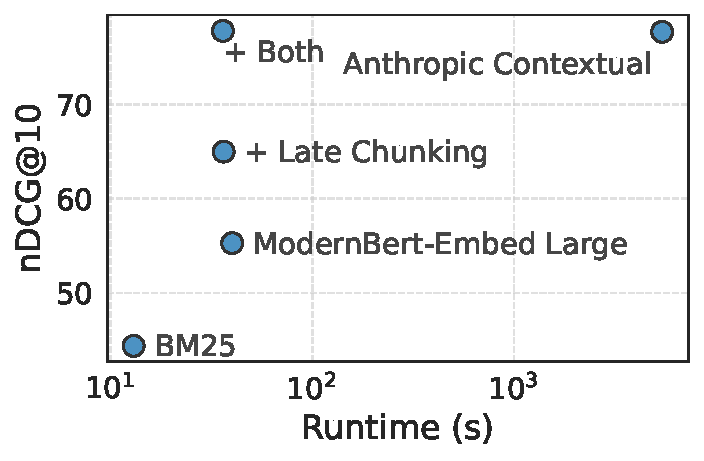
\includegraphics[width=\textwidth]{images/conteb_images/performance_vs_runtime.pdf}
%         \vspace{-3mm} % Reduce space between image and caption
%         % \caption{Retrieval performance vs. computational efficiency.}
%         \label{fig:pareto1}
%     \end{subfigure}
%     \hspace{1mm} % Reduce space between subfigures
%     \begin{subfigure}{0.49\textwidth}
%         \centering
%         \includegraphics[width=\textwidth]{images/conteb_images/lambda_seq.pdf}
%         \vspace{-3mm} % Reduce space between image and caption
%         % \caption{Alternative view of retrieval efficiency.}
%         \label{fig:pareto2}
%     \end{subfigure}

%     \vspace{-3mm} % Reduce space between subfigures and main caption
%     \caption{Side-by-side comparison of retrieval performance and computational efficiency. Our approach balances effectiveness and runtime optimally.}
%     \label{fig:pareto_combined}
% \end{figure*}

% Integrating conetxtual information makes a loagr diference (anthropoic contextual, both, and late chunking are largely ahead on all tasks, even wrt trained baseliens on the same data.


% Our training method unlocks extra performance, especiallu when it comes to integrating structuraml informatoip, (Insurance europa)

% our method is a the efficiency/performance frontier as shown in fig:pareto. While antrhopic's contextual yields slightly better performance, it requires expensive LLM summarization and contextualization which we do not require.

%
% \subsection{Not using doc wide context is suboptimal for retrieval}
\noindent\textbf{Document-wide context is essential.} As seen in \autoref{table:conteb:results}, methods leveraging contextual information widely outperform non-contextual methods across \emph{ConTEB} tasks. These results highlight the critical role of context-aware embeddings in improving retrieval performance in such settings, whether through untrained Late Chunking approaches or expensive context-aware reformulation approaches. 
As expected, the gap is even more notable in \emph{ConTEB}'s controlled setting experiments. 


% \textit{Our objective is to further boost the use of contextual clues through our training method to encourage improved information propagation across documents.} \manu{rework}


% \subsection{We can greatly improve upon existing contextualizations approaches with lightweight training}

% \noindent\textbf{In-Sequence Training.}
\noindent\textbf{Improving contextual information propagation.} Our results clearly show that \emph{InSeNT} variants outperform their untrained counterpart (+14.6 nDCG@10 for ModernBERT, +11.5 for ModernColBERT). Importantly, this is not due to the nature of the training data itself; the non-contextual ModernBERT model trained on the same data (ModernBERT + Training) does not improve upon the untrained baseline. Furthermore, the tasks that display the biggest improvements are the controlled setting tasks \textit{Insurance, Football}, that are explicitly designed to elicit information given in previous paragraphs, and that are out-of-domain w.r.t. our training set. 


\noindent\textbf{Late Interaction.} Interestingly, while LI models are good at long-context retrieving, they are poorly suited to out-of-the-box late chunking (-0.3 nDCG@10 w.r.t. ModernColBERT without LI). We posit that since token embeddings are never pooled, these models learn very local features and cannot leverage information from neighboring tokens. Once trained with our method, ModernColBERT+\emph{InSeNT} displays large performance gains across the board (+11.5 nDCG@10 w.r.t. ModernColBERT + Late Chunking), showcasing an increased ability to leverage external context.


\noindent\textbf{Context can add noise.} The \emph{CovidQA} task sticks out from the rest as untrained late chunking approaches severely degrade performance. Qualitative analysis, as well as the strong performance of the non-contextualized ModernColBERT method, indicate that the query-chunk pairing are often very extractive and match on technical medical terms, thus rendering context less useful. Our results show that naively applying late chunking in this setting adds noise and leads to notable performance drops (-21 nDCG@10), which are in large part recovered through our training method (+16 nDCG@10). 
%\manu{We perform toy viz to see this.}

% This indicates that the boosts achieved by through late chunking training are less about domain adaptation, and more about inducing meaningful information propagation between chunks. 

% To confirm performance gains in trained models are due to improved use of context rather than in-distribution training, XXX Trained on the exact same data, the non-contextual \textit{MB+Training} loses over 20 points to its contextual counterpart \textit{MB+InSeNT} on average.\manu{add details of this reference experiment to the appendix}

\begin{figure}[btp!]
    \centering
    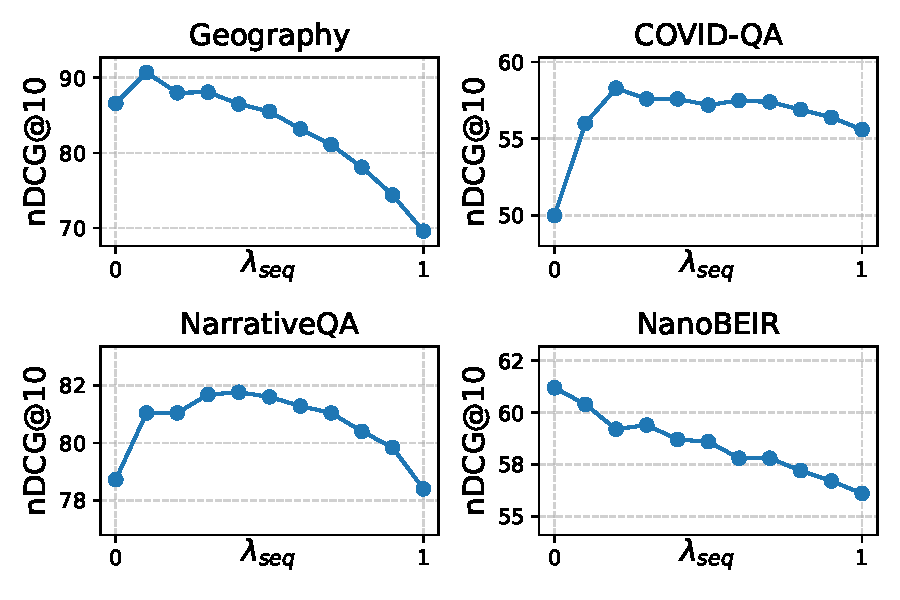
\includegraphics[width=0.65\textwidth]{images/conteb_images/lambda_seq_2x2.pdf}
    \caption[Importance of $\lambda_{seq}$]{\textbf{Importance of $\lambda_{seq}$}: Results for ModernBERT-Large trained with varying $\lambda_{seq}$. Optimal values depend on the task, but integrating both in-sequence and in-batch negatives is crucial to performance.}
    \label{fig:lambda_seq}
\end{figure}
\label{ablation_lambda_seq}

\noindent\textbf{$\lambda_{seq}$ matters.} The training objectives are to induce chunk representations to integrate document-level information (role of \emph{in-batch} negatives) while maintaining their specificity with respect to other same document chunks (role of \emph{in-sequence} negatives). By varying $\lambda_{seq}$ from \autoref{eq:loss_weighted}, we weight the importance of both objectives.

\noindent After training a series of models with varying $\lambda_{seq}$, we see on \autoref{fig:lambda_seq} that training with only in-sequence or in-batch negatives yields the worse results, and the optimal $\lambda_{seq}$ varies depending on the task. When documents need to be disambiguated between one another (\emph{NanoBEIR}, \emph{Geography}), up-weighting in-batch negatives seems optimal. On tasks where the challenge lies in locating information within a given document (\emph{NarrativeQA}, \emph{Covid-QA}), in-sequence negatives play a large role, but still need to be combined to in-batch negatives. Striking the optimal trade-off is thus very use-case dependent, and we opt for $\lambda_{seq}=0.1$ after tuning on the validation split of our training dataset.

% \textcolor{red}{These results interestingly build upon \sidecite{LateChunking}, highlighting the sensitivity of \textit{Late Chunking} to the weight of these joint objectives during training.}


% \noindent\textit{Our proposed training strategy improves upon LC by encouraging information propagation to favor inter-document separability (\emph{Football}, Geography), all the while limiting noise from the context, and making sure each document chunk embedding remains distinct from its neighbors (\emph{Insurance}, \emph{CovidQA}).} \manu{remove ? }\maxou{or move to conclusion}

\begin{figure*}
    \centering
    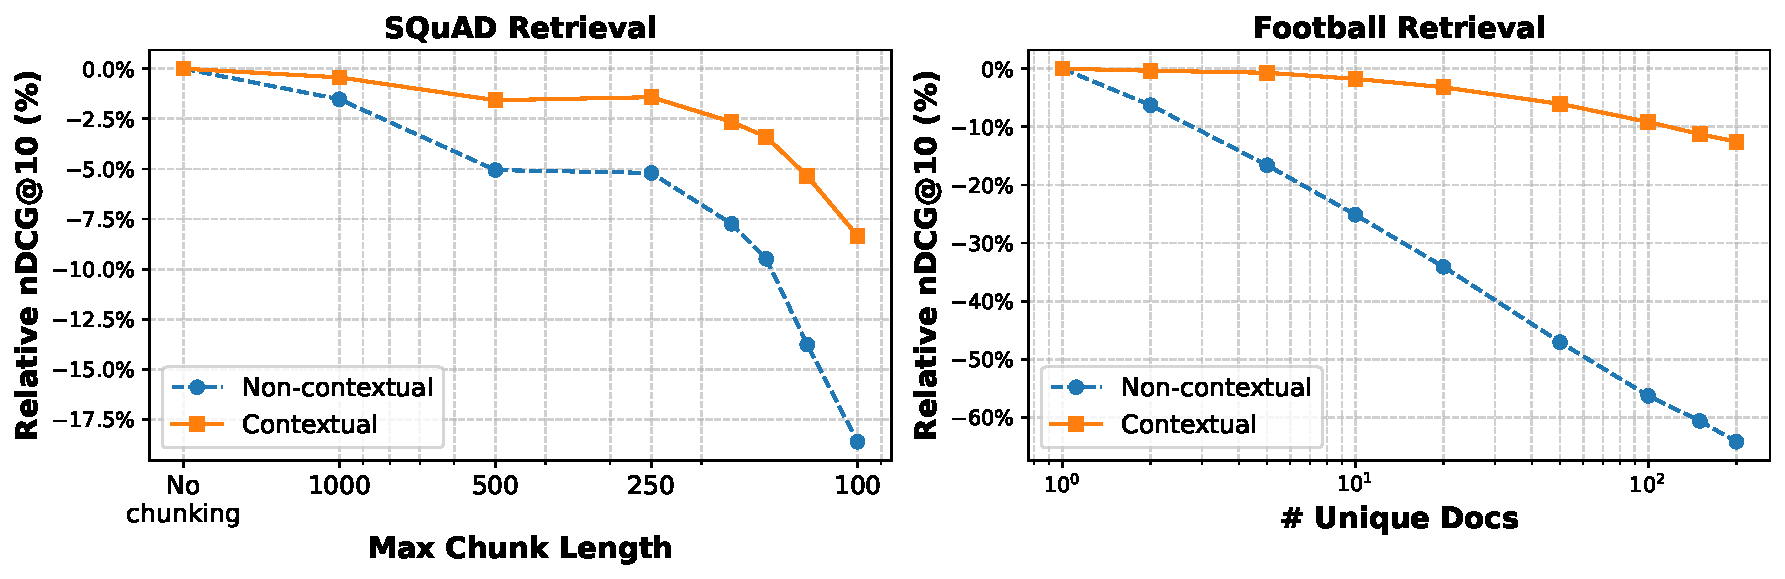
\includegraphics[width = 1\textwidth]{images/conteb_images/squad_football_retrieval.pdf}
    \caption[InSeNT robustness]{Contextualized models trained with InSeNT are more robust to aggressive chunking strategies that remove essential information from chunks (left), and scale better with corpus size and ambiguity (right).}
    \label{fig:robustness}
\end{figure*}


\noindent\textbf{Efficiency-Performance.} As shown in the Runtime column of \autoref{table:conteb:results}, our approach is very capable on contextual tasks, yet does not add much computational overhead. In fact, we find slight indexing speed improvements, attributed to our approach's reduced need for padding in-batch sequences of different lengths. While \textit{Anthropic Contextual} achieves sensibly similar performances on \emph{ConTEB}, it relies on costly LLM-based summarization and chunk reformulation, that are hardly scalable to huge corpora (120x slower).

\noindent\textbf{Short-Context Performance.} Careful hyperparameter tuning enables our best model to maintain strong performance on standard non-contextual benchmarks (\textit{NanoBEIR}), demonstrating that long-context optimization does not compromise short-context retrieval. Interestingly, LI models suffer from more degradation, which we posit is due to the original reliance on very local features modified through our training. Mixing in non-contextual "replay" data during training or merging models \sidecite{li2024improvinggeneraltextembedding_merging, modelmerging_lines} should further enable preserving the original embedding model's performances.

% \begin{figure}
%     \centering
%     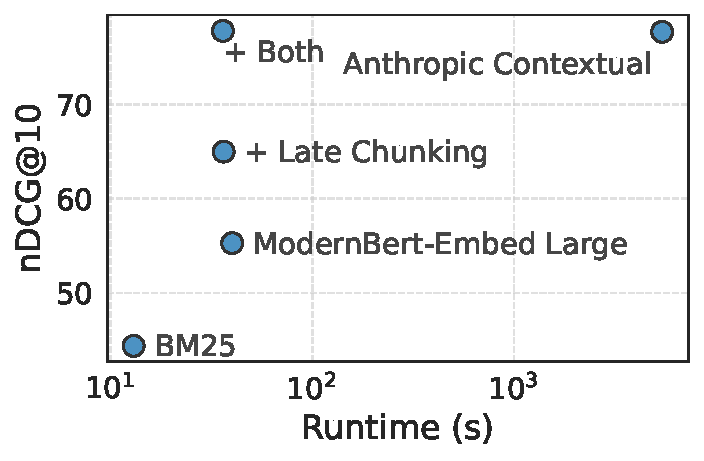
\includegraphics[width=0.45\textwidth]{images/conteb_images/performance_vs_runtime.pdf}
%     \caption{Comparison of retrieval performance versus computational efficiency across methods. Our approach achieves an optimal balance between effectiveness and runtime.}
%     \label{fig:pareto}
% \end{figure}


\section{Ablations}


% \noindent\textbf{Contextualized embedding training can be done without compromising the performance of the embedding model on short contexts}
% % our best models get better at long cxontext buyt stay good at beir. no tradeoffs !

% \noindent\textbf{Training on concatenated independent chunks hinders information propagation}
% % we train a model by concatenating short documents together from the nomic supervised dataset. we cluster these together as proposed by the paper cde-embeddings. We find evaluating these models on our benchmark severly degrases performance. Takeaway: essential to have long-context data that makes sense

% \noindent\textbf{The position in sequence matters}
% % evaluating if chunks in position 0 often have better representatioons  than later positionbs yierlds that yes. this is due to an encoder bis (needle in a haystackj). Takeaway: we must improve long context extension starategies in encoders to remove this bias (show this with nomic eval)


% \noindent\textbf{Preliminary contrastive finetuning with CLS token, then doing mean token pooling enable better transfer.}
% \section{Ablations}


% \subsection{\boldsymbol{\lambda_{seq}} matters.}

% \subsection{$\lambda_{seq}$ matters.}




\noindent\textbf{Robustness to chunking.}
We assess our method's robustness to poor chunking strategies using \emph{SQuAD} annotations.  Each originally self-contained chunk is split in multiple progressively smaller sub-chunks to while we keep track of the annotated answer span to identify the gold chunk. Eventually, these sub-chunks become too small to be self-contained and end up lacking sufficient information to be relevantly embedded on their own. \autoref{fig:robustness} (left) demonstrates that contextual embeddings greatly improves robustness w.r.t. suboptimal chunking. The model is able to elicit information from neighboring chunks to integrate contextual information within smaller sub-chunks, leading to a much more uniform retrieval performance across a wide range of chunk sizes.


\noindent\textbf{Robustness to corpus size.}
Common in the industry are templated documents that differ mostly by a key aspect (year, company name) but contain otherwise very similar information.
We study the dynamics of retrieval performance w.r.t. to the amount of similar documents in the corpus by computing scaling laws in which we iteratively vary the number of unique documents (composed of multiple chunks) in the corpus.
We observe in \autoref{fig:robustness} (right) that contextual embeddings scale vastly differently than their independently embedded counterpart. 
Intuitively, the greater the amount of similar documents and chunks in the corpus, the harder it is for a retrieval system to match the correct ones, but when embedding models are able to leverage external context, this effect is attenuated.



\noindent\textbf{Information Propagation.}
We experiment with concatenating semantically similar yet independent short chunks as "artificial" long documents. The resulting model is contextual as it uses late chunking, but exhibits performances in-line with non-contextual baselines (\textit{ModernBERT Large + Training}). We posit training on arbitrarily concatenated chunks, which by design are not contextually linked, teaches the model not to use information from neighboring chunks. This highlight the necessity of sourcing organic long-context data during training to induce correct training dynamics. Details in \autoref{table:nomic-results} in \autoref{app:res}.



% \subsection{Context-Aware chunks surpass Long-Context embeddings}

% \subsection{The Position in Sequence Matters}

% We investigate whether the position of a chunk in a sequence affects its representation quality. Our evaluation reveals that chunks appearing earlier in the sequence tend to have stronger representations compared to later ones. This bias is reminiscent of the \textit{needle-in-a-haystack} problem, where encoders struggle to maintain attention over longer spans. These findings indicate that current long-context extension strategies in encoders require further refinement to mitigate position-based biases. We illustrate this effect through evaluations on the \texttt{nomic} dataset.

% \subsection{Preliminary Contrastive Fine-Tuning with CLS Token, Followed by Mean Token Pooling, Enhances Transferability}

% \manu{See if useful} We experiment with a two-stage fine-tuning strategy: first performing contrastive learning using only the \texttt{[CLS]} token representation, followed by mean token pooling for final embeddings. This approach yields better transferability across retrieval tasks, as the initial contrastive step optimizes a global sequence representation before transitioning to a token-based aggregation strategy. Our results suggest that this hierarchical fine-tuning enhances generalization across both short and long retrieval tasks.


\section{Conclusions}
\label{section:conteb:conclusions_and_future_work}

In this work, we introduced \textit{ConTEB}, a benchmark designed to assess the effectiveness of retrieval models in leveraging document-wide contextual information. Our evaluation demonstrates that standard retrieval models struggle in context-dependent settings, while our proposed approach \textit{InSeNT}, which combines Late Chunking and a novel training methodology, performs strongly on \textit{ConTEB} without additional compute costs. % \textcolor{red}{These results prove the value of \emph{in-sequence} negatives in the training objective, and further bridge the gap towards practical utilization of the \textit{Late Chunking} paradigm.}
These insights build towards the broader development of the \textit{Late Chunking} paradigm in practice, and highlight the everlasting need for evaluation benchmarks that rigorously reflect how embedding models are used in real-world scenarios.
%By utilizing the ModernBERT architecture with late chunking and a weighted InfoNCE loss, we successfully integrate contextual knowledge into passage embeddings, leading to better retrieval performance with minimal computational overhead. 
% Our findings highlight the importance of contextual embeddings in enhancing retrieval accuracy, particularly in scenarios where document structure plays a crucial role.

\noindent\textbf{Future Work.} Scaling our approach with recent decoder models with extended context lengths (e.g., 1M+ tokens \sidecite{yang2025qwen251mtechnicalreport}) would enable embedding entire books or lengthy documents in a single forward pass, potentially unlocking new capabilities for large-scale document retrieval. It would also be interesting to observe the impact of our method on retrieval confidence \sidecite{gisserotboukhlef2024trustworthyrerankingsimpleeffective}. Finally, adapting our method to multi-modal embedding pipelines that have less control over the chunking strategy could further enhance retrieval systems in industrial applications with visually rich contextual documents \sidecite{faysse2025colpaliefficientdocumentretrieval, ma2024unifyingmultimodalretrievaldocument}. 
%Exploring new synthetic data generation strategies, and applying our training method with late interaction models \sidecite{khattab2020colbert} would also be an interesting avenue for future work.
% We hope our benchmark and findings serve as a foundation for future work in advancing context-aware retrieval systems.


% Talk about scaling this to decoders with 100K + token contexts. the vision is to emebd entire books in a single forward pass, this is a first step towards this vision. 
% another future step could be to apply this to embedding pipelines in which the system has less control on chunk construction, like page-level visual embeddings like colpali.


\section*{Limitations}

While our approach enhances retrieval performance in context-dependent settings, limitations persist.

\noindent\textbf{Context Length.} Our method is applied to long-context encoders that currently support sequences of up to 8k tokens. While we have shown performance can extrapolate to sequences of up to 32k tokens, scaling this approach to handle 1M+ token contexts with decoder-based models would be an interesting research avenue and presents significant compute and memory challenges. It notably requires rethinking the data construction processes to ensure longer documents are effectively leveraged.

\noindent\textbf{Non-contextual Performance.}
While our approach unlocks previously unattainable performance in contextual scenarios, it can come at the cost of slight short-context performance degradation. The optimal trade-off between non-contextual and contextual retrieval performance is highly usecase dependent \autoref{fig:lambda_seq} and can be parametrized by practitioners using the $\lambda_{seq}$ parameter. Other approaches may be promising such as model merging \sidecite{li2024improvinggeneraltextembedding_merging, modelmerging_lines}.


% \noindent\textcolor{red}{\textbf{Data Coverage.}
% While \textit{ConTEB} already covers a wide range of settings, we do believe there are still many avenues for future work. Increasing the language diversity (\textit{ConTEB} is English-only), integrating more domain-specific data with highly non-linear contexts (coding, legal texts) or experimenting with fixed context buffers (pre-pending Glossaries, or a List of Abbreviations, to texts) would further improve the coverage of contextual settings.}


\noindent\textbf{Data Generation.} The creation of training and evaluation data relies on existing datasets and semi-synthetic generation pipelines. However, a fully automated and scalable method for generating high-quality queries that effectively induce non-trivial context utilization remains an open challenge.

\noindent\textbf{Evaluation.} While our model demonstrates strong cross-domain performance, further validation in real-world applications, various use cases, and multiple languages is necessary to further assess its robustness and generalizability.


% \setchapterpreamble[u]{\margintoc}
\chapter{Trustworthiness Through Transparency: CroissantLLM}
% \chapter{\textit{CroissantLLM}: A Truly Bilingual French-English Language Model}



\begin{kaobox}[frametitle=Paper Abstract]

We introduce CroissantLLM, a 1.3B language model pre-trained on a set of 3T English and French tokens, to bring to the research and industrial community a high-performance, fully open-sourced bilingual model that runs swiftly on consumer-grade local hardware.
To that end, we pioneer the approach of training an intrinsically bilingual model with a 1:1 English-to-French pretraining data ratio, a custom tokenizer, and bilingual finetuning datasets. We release the training dataset, notably containing a French split with manually curated, high-quality, and varied data sources.
To assess performance outside of English, we craft a novel benchmark, FrenchBench, consisting of an array of classification and generation tasks, covering various orthogonal aspects of model performance in the French Language. Additionally, rooted in transparency and to foster further Large Language Model research, we release codebases, and dozens of checkpoints across various model sizes, training data distributions, and training steps, as well as fine-tuned Chat models, and strong translation models. We evaluate our model through the FMTI framework %\sidecite{bommasani2023fmti} 
and validate 81\,\% of the transparency criteria, far beyond the scores of even most open initiatives.
This work enriches the NLP landscape, breaking away from previous English-centric work to strengthen our understanding of multilingualism in language models.

\end{kaobox}

\section{Introduction}

% \pierre{do agree}
% \patrick{Is our main motivation training an fully open-source model OR training a small-but-competitive LLM for french-english? This intro basically just touches on the first, but I think we should also mention the second point (similar to TinyLlama). I think this/following paragraph should touch three problems with current LLMs: (1) LLMs (even "open-sourced" ones) are not fully open (2) models are mostly english-centric, and even multilingual models give little attention to the other languages (3) models focus on "compute-optimality" rather than "inference-optimality"}

% Transparency
% Large Language Models (LLM)\sidenote{See \autoref{sec:terminology} for a definition.} have taken over the Natural Language Processing (NLP) landscape in the past years.
Although a few proprietary models \sidecite{thakur_beir_2021, muennighoff_mteb_2022} are still considered to run ahead of the pack \sidecite{openai2023gpt4}, open weights models such as Llama \sidecite{touvron2023llama, touvron2023llama2}, Qwen \sidecite{bai2023qwen} or Mistral \sidecite{jiang2023mistral, jiang2024mixtral} are rapidly bridging the performance gap. However, widespread industrial and research adoption of such technology remains challenging for several reasons, including the lack of transparency in the data collection and training processes, the scarcity of existing resources outside of English, and the large-scale and costly nature of existing high-performing models.


\textbf{Lack of transparency.}
State-of-the-art models, both proprietary and open-weights are often designed and trained by heavily investor-backed companies, that aim to retain a moat by keeping their training data mix and strategy secret, hindering the rest of the field's ability to fully study and understand these models. 
% As such, very little is known about the data sources and training choices used for the open Llama, Qwen \sidecite{bai2023qwen} and Mistral \sidecite{jiang2023mistral, jiang2024mixtral} models, and even less so for the proprietary ChatGPT models from OpenAI, Claude from Anthropic, etc. 
This lack of transparency, ranging from training set composition to lack of evaluation or unclear usage policies, has been characterized by previous works, such as those by \sidecite{bommasani2023fmti} and \sidecite{casper2024blackbox}, pushing for full transparency as a key component for safe model development and use. 
% the idea is here is open --> seen -->   verified
The dangers of closed, non-auditable datasets have been exemplified by recent findings showcasing the potential dangers of dataset contamination, whether intentional \sidecite{hubinger2024sleeper} or not.\sidenote{\url{https://purl.stanford.edu/kh752sm9123}} Furthermore, legal questions arise surrounding data ownership in LLM training corpora \sidecite{nytimes, samuelson2023generative} and recent developments in the political landscape, regarding AI (EU AI Act, US senate hearings)\sidenote{\url{https://www.commerce.senate.gov/2023/9/the-need-for-transparency-in-artificial-intelligence}} have further emphasized the importance of transparent approaches, both from a legal perspective and to build user trust. 
% Furthermore, from a scientific perspective, the lack of any sort of reproducibility hinders progress in studying the mechanisms at work behind LLMs and 
% \pierre{you can talk about reproducibility and replicability} \manu{I don't get why, nothing is replicable at these scales?}
% mention sleeper agents paper, need to know what's in yur data for security reasons, csam images in public dataset  etc ...

% English Centric
\textbf{Bias towards English.}
Although the exact training mix of most well-performing LLMs is not publicly available information, most large models are trained on very English-centric corpora \cite{touvron2023llama}.
This is the consequence of the important amount of English resources compared to other languages, both in terms of data availability and benchmarks.
As could be expected, all publicly available LLMs display a large performance disparity between English and non-English languages when evaluated on downstream tasks \sidecite{bandarkar2023belebele}.
Moreover, cultural knowledge and biases are mechanically integrated through the training data, leading to models with greater knowledge of American events or biases \sidecite{bender2021dangers, santurkar2023opinions}. This puts non-English users at a disadvantage when it comes to language model usage and adoption.
While the non-English NLP community has produced multilingual datasets \sidecite{cerebras2023slimpajama, laurençon2023bigscience} and models \sidecite{scao2022bloom,mGPT} in the last few years, the available resources still largely lag behind English ones, hindering industrial adoption in non-English settings.


% Talk about compute vs inference optimal models
\textbf{Challenging to use at scale.}
Although benefits of scaling models to enormous sizes have been amply demonstrated in terms of performance \sidecite{hoffmann2022training, wei2022emergentabilitieslargelanguage, chowdhery2022palm}, scale comes at a large cost in terms of hardware requirements and inference speed. Download statistics on HuggingFace show the smallest Llama model \cite{touvron2023llama} to be the most adopted by the community, demonstrating the interest in small but capable models. 
LLM scaling laws demonstrate the diminishing returns of training a model of a given size past a certain amount of tokens. By continuing pre-training way past the compute-optimal threshold, performance has been shown not to saturate, enabling the training of ``inference-optimal'' models of high interest to the industrial and research communities \sidecite{sardana2023chinchillaoptimal}. It is still not fully understood how model performance continues to improve at these later stages of training.



% have a figure 1 with chat examples

\subsection{Contributions}

\begin{figure}
    % First figure
    \centering
    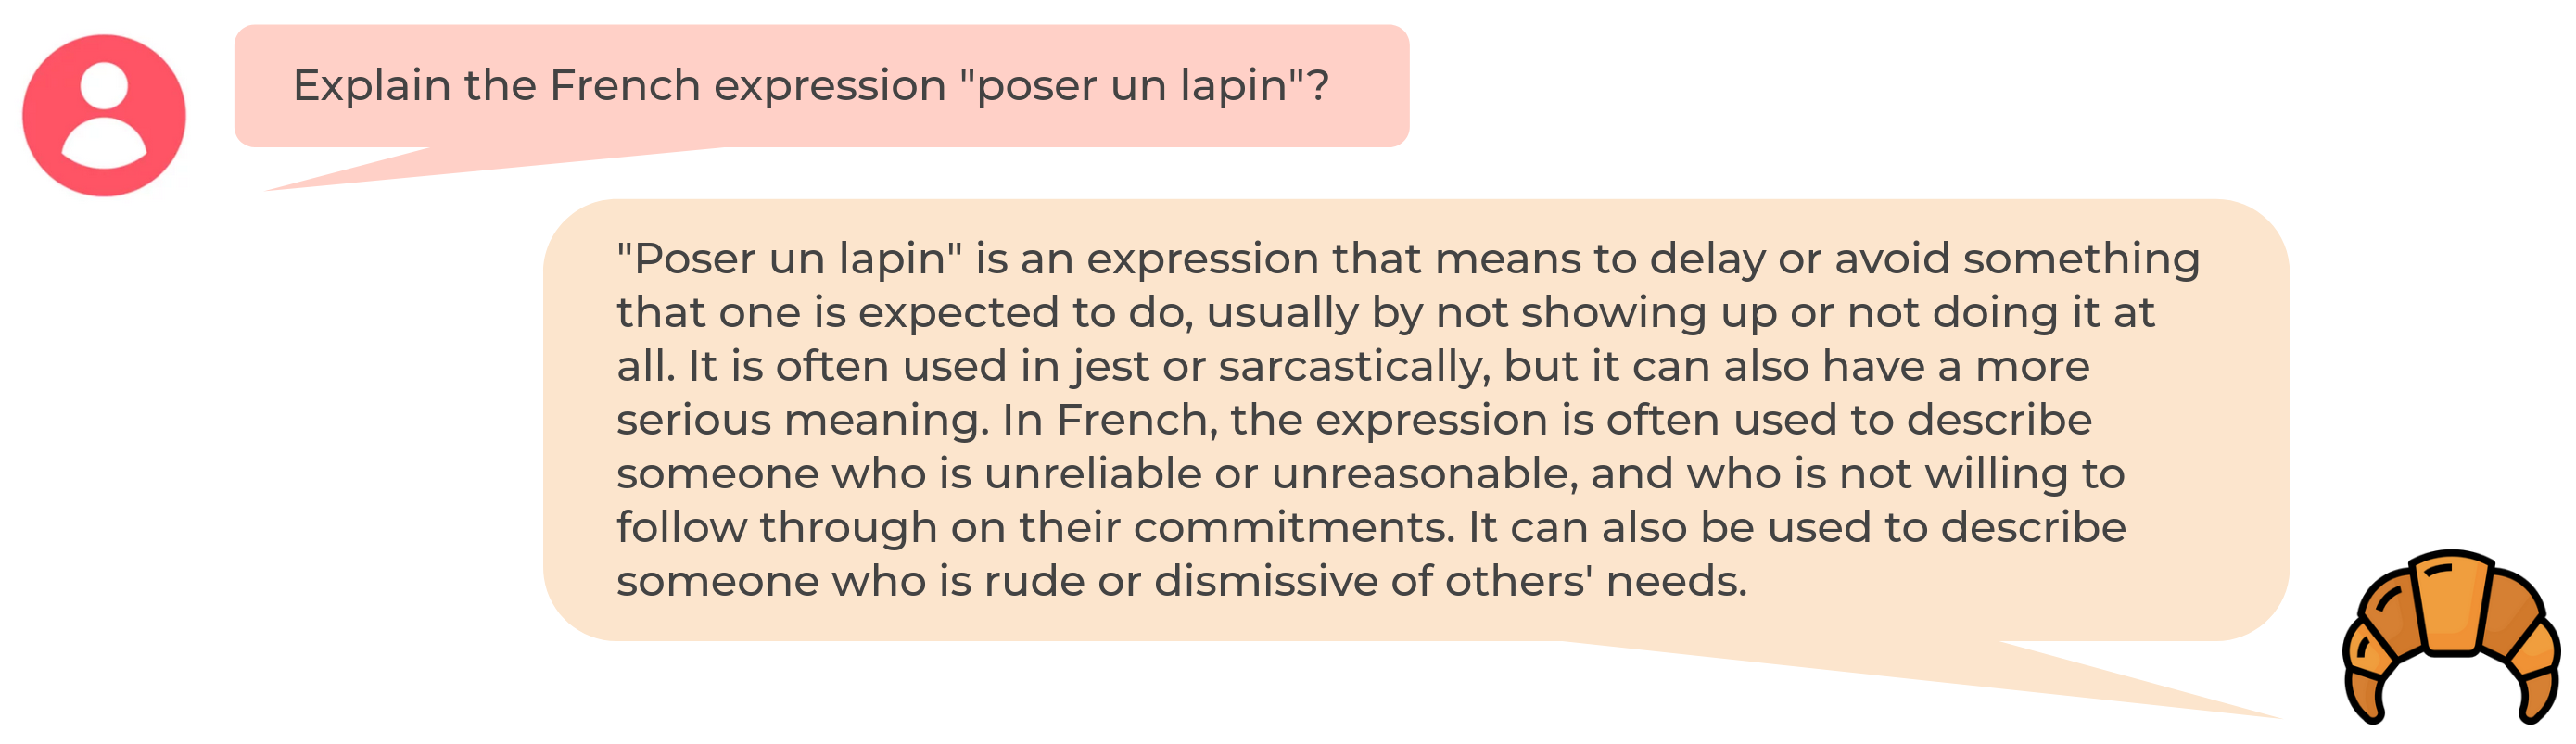
\includegraphics[width=\textwidth]{images/croissant_images/lapin.png}
    \caption[CroissantLLMChat example]{Conversation example with CroissantLLMChat}
    \label{fig:example}
\end{figure}




In this work, we attempt to bridge the aforementioned limitations and gaps.
Our main contributions can be summarized as follows.


\textbf{Contribution 1: Introduction of a highly-curated, diverse corpus in French.}
We collect and openly release a 303B token corpus spanning internet data, but also literary work, speech transcripts, legal and administrative documents, scientific articles, business-related documents, etc.
The corpus is distributed under permissive licenses, allowing commercial use with no restriction, and is heavily filtered, curated, and deduplicated. To our knowledge, it is the largest multi-source French language corpus released to date of sufficient quality for language modeling purposes\sidenote{By this, we imply of sufficient quality to train a language model (little OCR errors, high-quality text) and not exclusively composed of Internet data.}.
% FY: also https://huggingface.co/datasets/PleIAs/French-PD-Newspapers  -> yeah but  not usable for lm, OCR is shit, this corpus is worthless

\textbf{Contribution 2: Training CroissantLLM, a truly bilingual language model.} Nowadays, most models display some multilingual capabilities.
For example, Bloom has been trained to be massively multilingual \sidecite{scao2022bloom},
Llama contains a minor proportion of non-English data in its training set \cite{touvron2023llama}
and Qwen included a significative portion of Chinese data \cite{bai2023qwen}.\sidenote{Qwen-VL \cite{bai2023qwenvl} reports 77.3\,\% \& 22.7\,\% Chinese,  but no information is given for the Qwen base model.}
However, to our knowledge, outside of Chinese with a different alphabet \sidecite{zeng2022glm}, no work has studied or attempted to train a multilingual model of significant scale in which English is not the dominant training language.

In this work, we train a model on a 1:1 ratio of English to French with a tokenizer optimized for bilingualism.
Our end goal is to have a model less skewed towards English performance or cultural biases. 
% \caio{It was written "not skewed", but I think this is a too strong statement that could be attacked, I modified with "less skewed".}
We motivate this ratio by conducting careful experimentation on smaller model scales to uncover the trade-offs behind language distribution ratios.
We opt for a strategy enabling a ``best of both worlds'' performance in these two languages, as empirically validated by scaling law experiments. 
Experimentally, we show the importance of integrating data from another cultural source in the acquisition of cultural knowledge, underlining the importance of the effort. % \manu{update this sentence depending on angle}

% \manu{we show the impact of french data corpora on model knowledge --> importance of data in combatting cultural hegemony}

\textbf{Contribution 3: FrenchBench: A novel LLM benchmark for the French Language.} To evaluate models in French, we introduce a benchmark encompassing various tasks to assess factual knowledge, generative capabilities, language understanding, etc. This benchmark is constructed both from openly available datasets, as well as newly released manually annotated data. We evaluate and report results for our models as well as other models with French-speaking capabilities.\sidenote{Code for evaluation is available at \url{https://github.com/EleutherAI/lm-evaluation-harness}}\footnote{Another complementary initiative has been led for French model evaluation and released concurrently in \cite{bawden:hal-04435371}}


\textbf{Contribution 4: Releasing high-performing, inference-optimal models for the industrial community, together with a wide range of resources for the research community.}
The models we train are all released under open licenses. Our largest model is trained on a 2300:1 token to parameter ratio (115 times longer than a Chinchilla Optimal 1.3B model) leading to very strong performance in its size category.
We show that model performance on downstream tasks continues to dramatically improve with lengthened pre-training runs, although model perplexity does not significantly improve.
We release all checkpoints for all model sizes, as well as the exact training data seen at every step for research purposes.\sidenote{Training data indexing order will be released in a second stage.} These models are extremely efficient to run, leading to low-latency, energy-efficient on-edge inference, even on low-resource devices such as phones or personal computers.
These releases\sidenote{Code for dataset collection and filtering is available at \url{https://github.com/ManuelFay/llm-data-hub}. Code for model training is hosted at \url{https://github.com/CoderPat/croissant-llm-training}. Datasets and model checkpoints are available at \url{https://huggingface.co/CroissantLLM}.} are motivated by a commitment to transparency to allow research and reassuring users for industrial deployment: our models comply with 81\,\% of criteria listed by the Foundation Model Transparency Index \sidecite{bommasani2023fmti} (see Section~\ref{sec:transparency}). 



The CroissantLLM initiative aims to adress the aforementionned limitations of current models through the release of an inference-optimized, small but capable model that performs well outside of English settings, and that is designed to be as open and transparent as possible. Beyond facilitating industrial LLM adoption and unlocking new generative model use cases, this project is also a proven platform for researching LLMs and kickstarting future pretraining efforts 
\cite{martins2024eurollmmultilinguallanguagemodels, meeus2024copyrighttrapslargelanguage, shilov2024mosaicmemoryfuzzyduplication, meeus2024sokmembershipinferenceattacks}.

% This opens up new perspectives, on the relevance of validation perplexity as a proxy measure for "good" models, and on the benefits of long pretraining runs. 
% Our resulting model displays strong performance for its size, outperforming larger models trained on less tokens while being less memory intensive and faster, showcasing the industrial interest in training small yet effective models.

% \FloatBarrier doesn't work

% \clearpage
\section{Data}
The dominance of the English language in the training data of most current models is undeniable. While multilingual models like Llama leverage some non-English data \cite{touvron2023llama}, it corresponds to only a minor part of the corpus, leading to a significant drop in performance across non-English data, with noticeable ``American'' bias \sidecite{santurkar2023opinions, 10.1145/3597307}.
% (Caio) the sentence below is incorect, both French and English are indo-european languages
%This work aims to offset this trend by using a more balanced bilingual corpus comprising English and French, a rich language from a distinct language family. \caio{What do you mean? Both English and French are indo-european languages, it is the same family. French has a "richer" morphology than english (but you can't just say "rich language"), maybe focus on this point instead, but we need to find a citation to justify this claim.}
This work aims to offset this trend by using a more balanced bilingual corpus comprising English and French, as well as additional code data.
Although both languages belong to the Indo-European language family, they exhibit different morpho-syntactic structures\footnote{For example, pronominal objects are placed before (resp.\ after) the verb in French (resp.\ English), both languages have different noun phrase constructions (``la commission européenne'' vs.\ ``the European commission''), etc.} and French has a richer morphology.\footnote{For example, English has 5 verb forms whereas French has 48, French has explicit inflections for grammatical genders, etc.
However, note that only English adjectives have morphological constructions for expressing comparison (\emph{e.g.}\ easy, easier, easiest). We refer to WALS for more details, \emph{e.g.}\ \url{https://wals.info/feature/21B##2/26.7/152.4}
} We study whether this corpus helps in reducing biases, enabling more varied knowledge sets, and unlocking non-English performance.

A variety of sources are integrated into our corpus, including carefully filtered internet data and high-quality data from a range of sources, all devoid of restrictive licenses ensuring complete openness of the data and the trained model. Data statistics are available in Table~\ref{tab:tab_tot}. As further detailed in \ref{sec:final_data}, our data corpus contains different amounts of unique English, French, and Code tokens. We obtain our balanced training corpus by upsampling French, Code, and English data with different sampling ratios, such that no performance loss is to be expected \sidecite{muennighoff2023scaling}.


\begin{table*}
    % \footnotesize
    \centering
    \begin{tabular}{lllllll}
    \toprule
     & Size (GB) & Docs. (M) & Tokens (B) & Token/Doc & Sampling Ratio & \# tokens (B) \\
    \midrule
        French & 1258.70 & 376.27 & 303.51 & 806.63 & 4.09 & 1240.08 \\
        English & 2351.13 & 591.23 & 655.64 & 1108.94 & 1.89 & 1240.09 \\
        Code & 366.87 & 81.90 & 141.43 & 1726.76 & 2.04 & 288.92 \\
        Parallel & 113.91 & 408.03 & 35.78 & 87.68 & 6.13 & 219.26 \\
        \midrule
        \textbf{Total} & 4090.61 & 1457.43 & 1136.35 & 779.70 & 14.15 & 2988.35 \\
    \bottomrule
    \vspace{0.2mm}
    \end{tabular}
    \caption[CroissantLLM data mix]{Final Data mix for CroissantLLM training}
    \label{tab:tab_tot}
\end{table*}


The scrapping and processing code are available in our code base.\sidenote{\url{https://github.com/ManuelFay/llm-data-hub}} The license information of all datasets used is given, all allowing for permissive commercial use.

\subsection{French Data}


Table~\ref{tab:tab_fr} lists the source and some information regarding the French corpus. Details about the data sources are expanded further below.


\textbf{Web Data.} We collect internet data from various web scraps (Oscar \sidecite{abadji-etal-2022-towards}, mC4 \sidecite{xue2021mt5}), leveraging the CulturaX corpus \sidecite{nguyen2023culturax} for heuristic and perplexity filtering, as well as exact and fuzzy deduplication. In total, this represents over 363 million webpages and more than 292 billion tokens, that we split using our custom tokenizer fitted on equal amounts of French and English data.\footnote{The mC4 corpus \url{https://huggingface.co/datasets/allenai/c4} is released under the ODC-BY licence \url{https://opendatacommons.org/licenses/by/1-0/} whereas Oscar \cite{abadji-etal-2022-towards} does not claim data ownership, provides an opt-out strategy for data inclusion, and filtering metadata is released under the Creative Commons CC0 license.\url{https://creativecommons.org/publicdomain/zero/1.0/}}

We ensure data is of good quality and correctly tagged in French through sampled manual inspection and confirm French-speaking countries are well represented within the dataset. Notably, we include several news sources scrapped from Belgium, Switzerland, Canada, and Lebanon, as well as multiple African countries (Senegal, Morocco, Algeria, Cameroon, etc.) \sidenote{Contrary to certain languages such as Arabic or Portuguese in which the language differs greatly depending on the country, the written French language in these countries are largely similar with only a minor share of regionally introduced syntax and expressions}
% desvrive the toxicuty filtering

\textbf{Legal and Administrative Data.}
We introduce 5.3B tokens of data from the French government's open data initiative, ranging from legal tasks to parliamentary discussions and financial transcripts (\emph{e.g.}\ legal and administrative jargon). These texts originate from 13 different datasets (the OpenData corpus) and were collected from the French government's open data platform.\sidenote{Data is released at \url{https://echanges.dila.gouv.fr/OPENDATA/} with the ETALAB open license \url{https://www.etalab.gouv.fr/wp-content/uploads/2017/04/ETALAB-Licence-Ouverte-v2.0.pdf}}
To ensure other French-speaking countries are represented, we add 68M tokens of data from Swiss legislation retrieved from government sources.
We perform steps to process, filter, and run exact deduplication on these documents.

\textbf{Cultural Data.} We introduce cultural data from various sources. Notably, we retrieve all Project Gutenberg \sidecite{projectgutenberg} books in the French language as of October 2023, corresponding to books released in the public domain (302 million tokens). We also download and aggressively filter manuscripts and documents from the French National Library (Bibliothèque Nationale de France), and filter for documents that belong to the public domain, have undergone an OCR process, and are of high quality.\sidenote{Metadata is licensed under Open Etalab license \url{https://gallica.bnf.fr/edit/und/conditions-dutilisation-des-contenus-de-gallica}} To filter out low-quality OCR documents, we implement custom heuristics which we release within our code base.
We run all documents through perplexity filters using KenLM 5-grams\sidenote{\url{https://github.com/kpu/kenlm}} fitted on the French Wikipedia split, and discard documents with perplexity values that are too high (noisy) or too low (repetitive patterns).
Thresholds are set through a manual verification process.
We deliberately choose to be aggressive in our filtering to ensure only high-quality data is kept and discard the largest portion of the original corpus, keeping about 27M tokens. We choose not to keep any data from the newspaper archives, as the OCR transcription is often too noisy. Additionally, we introduce famous public domain French poems custom scrapped from a French poetry website,\sidenote{\url{https://www.poesie-francaise.fr/}} and run a set of podcasts through a high-quality speech-to-text model to obtain a textual transcription. This process is hard to scale and data splits from these sources are limited in quantity.
Data from the OpenSubtitles\sidenote{\url{https://opus.nlpl.eu/OpenSubtitles2016.php}} initiative is integrated, corresponding to 41.8 million tokens originating from movie subtitles.\sidenote{\url{https://www.opensubtitles.org}} Finally, we add the French data from Wikisource collected as part of the BigScience initiative \sidecite{scao2022bloom} and obtain 2.7 billion tokens from the process.\sidenote{Licensed under CC BY-SA 4.0, \url{https://en.wikisource.org/wiki/Wikisource:Copyright_policy}}


\textbf{Encyclopedia Data.} To introduce high-quality factual data to the training corpus, we integrate the French Wikipedia split from November 2023.\sidenote{\url{https://huggingface.co/datasets/wikimedia/wikipedia} with a CC-By-SA 3.0 license} This corresponds to the latest knowledge cutoff in the training data. In total, more than 2.5 million articles are used, spanning more than 2 billion tokens.

\textbf{Industrial Data.} We scrap high-quality and publicly available data from industrial PDFs via a manually crafted list of websites, from large French and French Canadian (Quebec) companies to government agencies. This business-focused data boosts performance on a series of downstream applications related to industrial NLP. We collect over 36000 PDF multi-page documents and filter them through carefully crafted heuristics, followed by aggressive perplexity filtering.\sidenote{Data is public internet data that we release under MIT license with an opt-out scheme \url{https://huggingface.co/datasets/manu/illuin_layout_dataset_text_only}}.
In total, we obtain over 290000 documents and 191 million tokens. 

\subsection{English Data}

Our English data is primarily drawn from the SlimPajama corpus \sidecite{cerebras2023slimpajama}, excluding copyrighted documents.
Splits per data source are detailed in Table~\ref{tab:tab_en}. 

\textbf{Internet Data.} Similarly to the French dataset, we rely on carefully filtered content from an assortment of internet sources, including miscellaneous web pages and blogs. The filtering process includes heuristics and perplexity filtering, as well as large-scale deduplication \sidecite{cerebras2023slimpajama}. The SlimPajama corpus includes internet data from the CommonCrawl\sidenote{Common Crawl license \url{https://commoncrawl.org/terms-of-use}} and C4\sidenote{ODC-BY license} web scraps, as well as data sourced from Github textual content\sidenote{Only content under MIT, BSD, and Apache licenses are kept} and the StackExchange forums.\sidenote{CC-By-SA 4.0 license \url{https://archive.org/details/stackexchange}}
% desvrive the toxicuty filtering

\textbf{Miscellaneous.} Other non-internet-based data sources are included in the SlimPajama dataset, such as scientific articles from Arxiv\sidenote{\url{https://arxiv.org/}, with author opt-out options} and English documents from Wikipedia.\sidenote{CC-By-SA 3.0 license} The SlimPajama dataset is also comprised of the ``Books'' subcorpus, obtained by downloading all book documents from Bibliotik.\sidenote{\url{https://huggingface.co/datasets/the_pile_books3}}
Some of the documents within this last corpora have been flagged by their owner as proprietary data. We filter out all documents from this subcorpus, and replace them with data from the open-source Project Gutenberg \sidecite{projectgutenberg} English books under public domains.\sidenote{ From \url{https://huggingface.co/datasets/pg19} with an Apache 2.0 license}

\textbf{Gutenberg Canaries.} To assess model memorization to inform about the risks of including private or sensitive data within the training set, we stress test the model by including ``canaries'' \sidecite{carlini2019secretsharer}. These correspond to samples that have been intentionally modified and/or repeated and included within the model training set, and that will enable a posteriori evaluation of the model capacity to memorize data in a ``worse than worst-case'' situation.\sidenote{This work is led in parallel to the CroissantLLM project and findings will be independently published.} In total the canaries represent 555 million tokens, representing less than 0.04\,\% of the total tokens seen during training.

% Mention the canaries briefly



\subsection{Code Data}

In line with most recent models \cite{chowdhery2022palm, scao2022bloom, touvron2023llama}, we integrate code data into our training corpus. Notably, previous work shows that code data benefits natural language tasks and can be particularly useful in data-constrained settings \sidecite{muennighoff2023scaling}. Therefore, we include 140B tokens of code data in several common programming languages.
Splits and number of tokens are detailed in Table~\ref{tab:tab_code}.

\textbf{The Stack \& StarCoder.} We rely on the efforts of the StarCoder project \sidecite{li2023starcoder}, and use their high-quality filtered code data from The Stack corpus \sidecite{kocetkov2022stack}.\sidenote{Data are drawn from various sources and falls under 193 different permissive licenses. We use the version $1.2$ of the corpus, which has been filtered with respect to data owners opt-out option information.}
We keep only high-resource programming languages (Java, Javascript, Python, C, C++, SQL) and Jupyter notebooks, as well as a few samples of formatted data (JSON, Tex) and scripting languages (shell scripts, Dockerfiles).


\textbf{Extra Python code.}
We extend the corpus with several other sources of Python code due to the popularity of the language in the community.
Firstly, we add Pypi packages from recent code dumps, that are filtered to keep only Python and Jupyter files.\sidenote{\url{https://huggingface.co/datasets/vikp/pypi_clean}}
Secondly, in order to promote high-quality problem-solving-centered code, we integrate 1.2B tokens of Python3 data from competitive coding contests \sidecite{doi:10.1126/science.abq1158} under CC-By-4.0 license.
Lastly, following the success of learning from textbooks \sidecite{li2023textbooks}, we add commented Python code constructed by combining code and text cells from Jupyter Notebooks through the CodeParrot initiative.\sidenote{\url{https://huggingface.co/datasets/codeparrot/github-jupyter-code-to-text} Apache 2.0 license }


\subsection{Parallel Data}
%\pierre{ici il faudra cite le papier de Palm qui montre que incorporer des données parallel aide el trainin \url{https://arxiv.org/pdf/2305.10403.pdf,}, \url{https://aclanthology.org/2023.acl-long.524.pdf} }
Following previous work \sidecite{anil2023palm},
we incorporate vast quantities of parallel data, in our case high-quality English-French translation pairs, in order to improve the multilingual capabilities of the model \sidecite{briakou-etal-2023-searching}.

\textbf{Opus.}
We extract subsets of sentence pairs spanning multiple domains from the OPUS corpus \sidecite{opuscorpus}.\sidenote{Free license \url{https://opus.nlpl.eu/}}
Statistics are described in Table~\ref{fig:opus}.
In total, we include 400 million parallel sentences and about 36 billion tokens. The data is filtered through a rigorous cleaning pipeline:
(1)~BiFixer \sidecite{ramirez-sanchez-etal-2020-bifixer}\sidenote{\url{https://github.com/bitextor/bifixer}} is first used to remove duplicate data through fuzzy matching techniques;
(2)~BiCleaner\sidenote{\url{https://github.com/bitextor/bicleaner}} is then used to filter data using heuristic and perplexity filters;
(3)~finally, the state-of-the-art NMT quality estimator CometKiwi \sidecite{rei-etal-2022-cometkiwi} is used to keep only top quality translation pairs. 
 

\textbf{Theses.} To incorporate versatile academic and scientific language, we augment our dataset with French theses abstracts along with their author-generated English translations. This corresponds to 95000 documents and more than 80 million high-quality tokens.\sidenote{Data licensed under Etalab open license \url{https://www.etalab.gouv.fr/wp-content/uploads/2017/04/ETALAB-Licence-Ouverte-v2.0.pdf}}

\textbf{Song Lyrics.}
Our dataset integrates song lyrics in both French and English, scrapped from a specialized community-driven lyrics translation website.\sidenote{\url{https://www.lacoccinelle.net}, with opt-out options for data owners and community-contributed translations under free-use license.}
As such, our model is trained with radically different linguistic styles (\emph{e.g.}\ colloquialism), and the wide range of topics can help the model to capture cultural nuances. 
Lyrics have been translated by hand by the website community. With a total of 70k songs, we have built up a corpus of 53M tokens covering different periods (80s, 90s, 20s, etc.) and musical genres (rap, rock, jazz, etc.) To preserve colloquial expressions and cultural subtleties, we have not filtered song lyrics for explicit content. We validate the original language metadata of the songs through Google's language-detection algorithm. 

% \pierre{sur les data il font des trucs come \url{https://arxiv.org/pdf/2303.03915.pdf} fig 1 ca peut être bien}


%\clearpage
\section{Training}

Our main goal was to train a high-performing, yet resource-friendly bilingual model while optimizing performances across both languages. To focus on the specific challenges of the bilingual paradigm, we rely on previous work to motivate many of our design and hyperparameter choices \sidecite{touvron2023llama2}.

\subsection{Model Architecture}
% Patrick
We use the Llama architecture \cite{touvron2023llama}, a decoder-based transformer, trained with rotary position encodings \sidecite{su2023roformer} and a context length of 2048. 
We construct 4 different model sizes by jointly scaling the number of attention heads, hidden size, and hidden layers. Table~\ref{tab:model_scaling} summarizes the sizes of each model in the family.

\begin{table}
    \centering
        \begin{tabular}{llllll}
        \toprule
        Model & Params (M) & Layers & Hidden size & Inter. size & KV heads \\
        \midrule
        XXS & 100.7 & 6 & 1024 & 4096 & 8 \\
        XS & 202.5 & 12 & 1024 & 4128 & 8 \\
        S & 341.5 & 12 & 1536 & 4128 & 12 \\
        \midrule
        Base & 1214.3 & 24 & 2048 & 5504 & 16 \\
        \bottomrule
        \vspace{0.2mm}
        \end{tabular}

    \caption[Scaling law model info]{Model information for scaling laws. Parameter count excludes embedding and output parameters.}
    \label{tab:model_scaling}
\end{table}



\subsection{Tokenizer}

Most LLM tokenizers are fitted on English-centric corpora with an information-theoretic optimization objective, for example, Byte-Pair encoding \sidecite{sennrich2016neural} or Unigram \sidecite{kudo2018subword}, leading to good fertility\sidenote{See \autoref{sec:terminology} for a definition.} values (low token per word ratio) on English text, but high fertility in other languages. These phenomena make processing in other languages slower and more costly \sidecite{rust2021good}. Furthermore, subword splits in non-English languages mechanically carry less semantical meaning, potentially being a factor in the degraded performance of models on non-English languages \cite{rust2021good}.

\textbf{Tokenizer training.} We fit our CroissantLLM tokenizer on a corpus of 100B high-quality tokens, with splits of English, French, and code data. We use SentencePiece\sidenote{\url{https://github.com/google/sentencepiece}} to train a Byte-Pair Encoding tokenizer with a vocabulary size of 32000 tokens,  100 special placeholder tokens, whitespace separation, and byte fallback, inspired by \cite{touvron2023llama, jiang2023mistral}. The data corpus used to fit the tokenizer is made available,\sidenote{\url{https://huggingface.co/datasets/manu/tok-corpus-shuffled}} and notably contains large amounts of French data to skew the vocabulary construction process towards optimizing for French as well.

\textbf{Improved fertility rates.} The focus on English, French, and Code enables the CroissantLLM tokenizer to display smaller fertility rates on French texts than the Mistral and Llama models with similar vocabulary sizes, all the while also displaying slightly smaller rates than both in English and Code (Figure \ref{fig:tok_fertility}). This is due to the multilingual support of both Llama and Mistral tokenizers which need to allocate some vocabulary tokens to frequent character patterns from other languages.
Roughly, the Llama tokenizer is 17\,\% less token efficient at encoding French internet data, and up to 40\,\% less efficient on clean encyclopedia French texts, implying that the 303B unique French tokens in our data training set correspond to more than 360B tokens with the Llama tokenizer. This enables us to pack more data in fewer tokens, leading to improvements in training and inference efficiency.

\begin{figure}
    % First figure
    \centering
    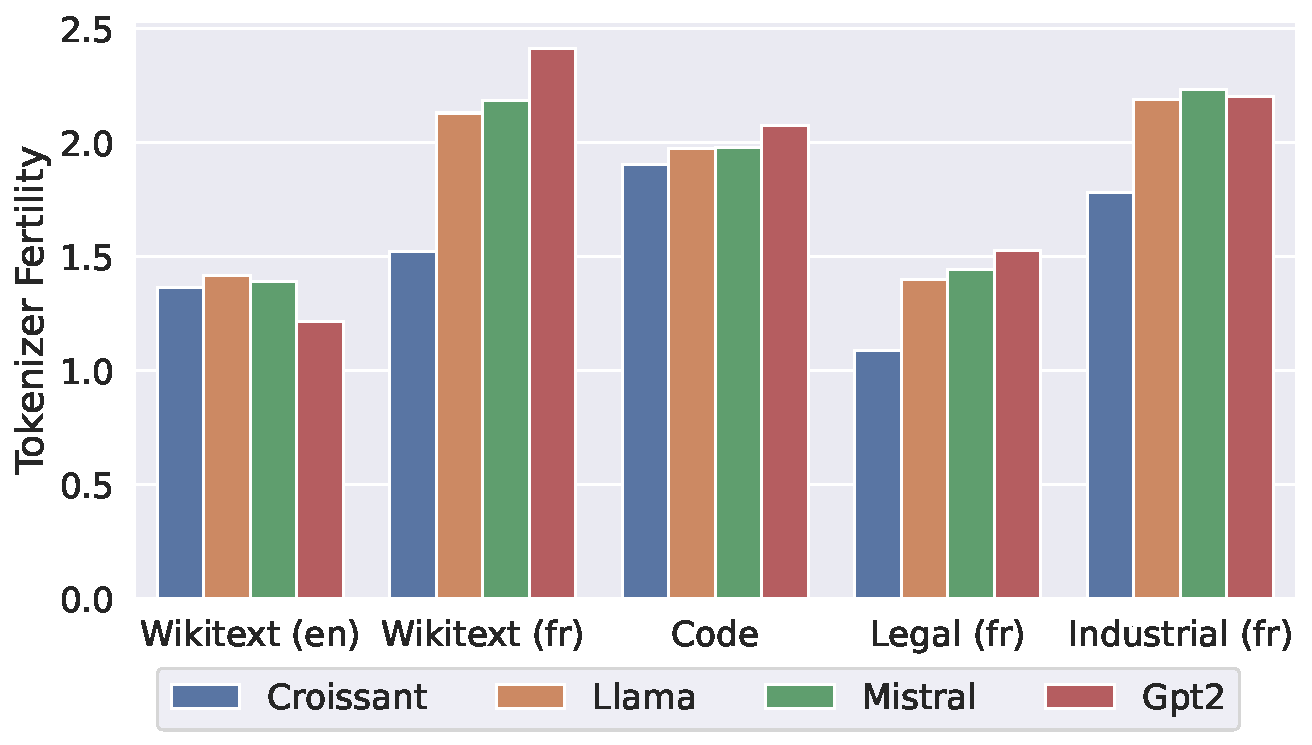
\includegraphics[width=0.8\textwidth]{images/croissant_images/fertility.pdf}
    \caption[Fertility across tokenizers]{Fertility on unseen test sets using various tokenizers. Lower is better.}
    \label{fig:tok_fertility}
\end{figure}


\subsection{Selecting an optimal language ratio}

A crucial question when training a bilingual model is how to effectively \textit{weight} data from the two languages to achieve a good trade-off between performance in both. While, intuitively, training on an equal mixture of English and French data may seem to be the obvious solution, differences in data quality available for each language coupled with transfer learning dynamics between both languages could imply that a balanced mix might be sub-optimal. However, training multiple models with different data mixes for comparison is prohibitively expensive.

To offset this computational cost, we leverage recent findings on scaling laws \sidecite{scaling-laws-lm} that show that we can predict the performance of our model by training smaller models on the same dataset. In particular, \sidecite{pmlr-v202-fernandes23a} found that, for \textit{multilingual} models, by training smaller models with varying weights for each language in the data mix, one can fit a \textit{multilingual, joint} scaling law that can predict the language performance trade-off of larger models, even for novel language weightings not encountered during the fitting of the scaling law. 

As such, we fit a joint scaling law as described by \cite{pmlr-v202-fernandes23a} for each language, by training 3 smaller model sizes on 3 different data mixes with varied ratios of English and French data (keeping the amount of Code data fixed). The corpus for these scaling law experiments is a subsampled variant of the larger corpus and is detailed in Appendix \ref{sec:scaling_data}. We define 3 data mixes by varying the language sampling ratio:
(1) \textbf{equal} containing 40\,\% English data, 40\,\% French data and 20\,\% Code data;
(2) \textbf{frplus} containing 20\,\% English data, 60\,\% French data and 20\% Code data;
and (3)  \textbf{enplus} containing 60\,\% English data, 20\,\% French data and 20\,\% Code data. We then trained a 1.3B model on these subsets of the data for one of the data mixes to validate their predictive power.


% \patrick{should I put the scaling law form here? The GPT-4 tech report didn't even bother...}

\begin{figure*}
    % First figure
    \centering
    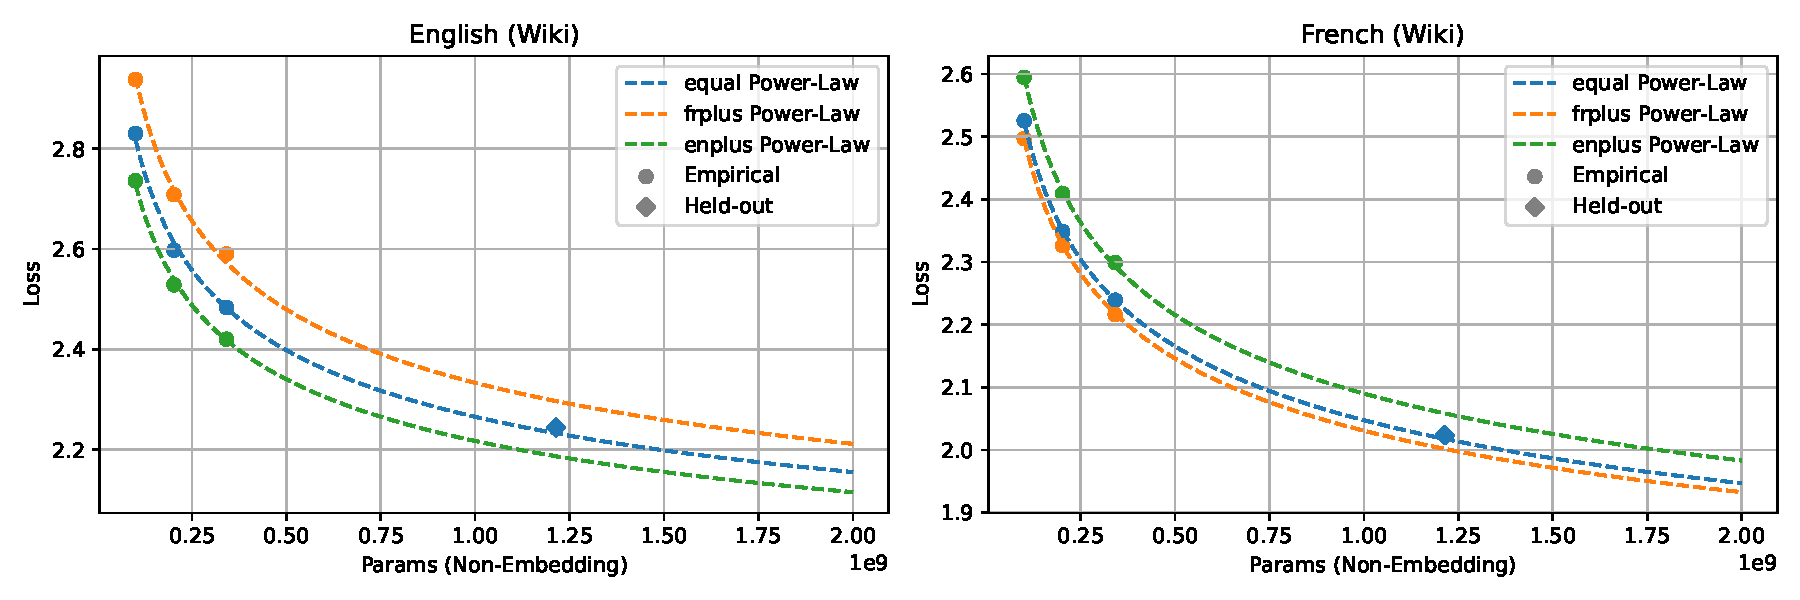
\includegraphics[width=0.95\textwidth]{images/croissant_images/scaling_laws_croissant_wiki.pdf}
    \caption[Test loss scaling evolution]{Evolution of test cross-entropy loss with model size in English (left) and French (right), for the \textit{wiki} domain, as well as the fitted joint scaling laws,}
    \label{fig:scaling_laws_fit}
\end{figure*}

\begin{figure*}
    \centering
    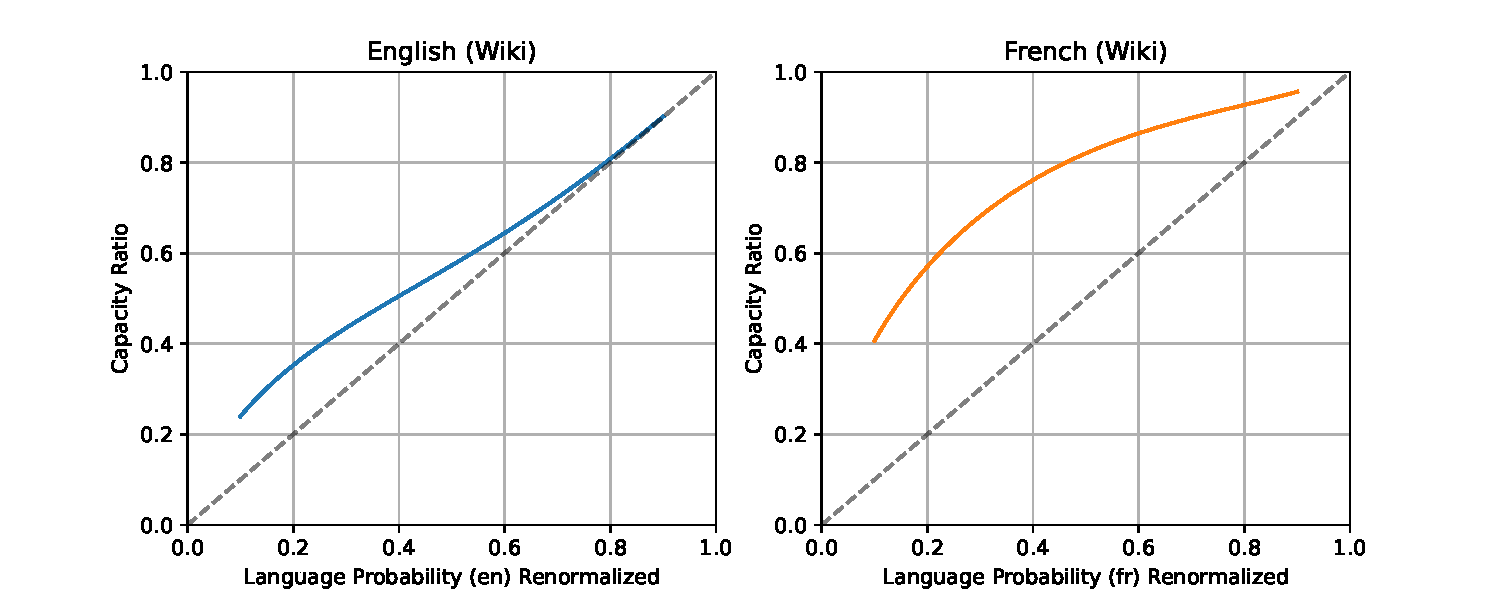
\includegraphics[width=0.95\textwidth]{images/croissant_images/scaling_laws_capacity_wiki.pdf}
    \caption[Effective capacity ratio]{\textit{Effective capacity ratio} (as predicted by our fitted joint scaling law) for English and French as we change the weight of each language.}
    \label{fig:scaling-laws-capacity}
\end{figure*}

\autoref{fig:scaling_laws_fit} shows the performance predicted by jointly-fitted scaling laws as we scale the model and vary the language weightings on the Wiki data validation split.
%composed of wiki data, as well as the empirical performance obtained from the trained models.
First, we see that the fitted scaling law is able to predict the performance of the larger model almost perfectly. Secondly, changing the weight of each language in training has a non-symmetrical impact on language performance: by increasing the (relative) weight of French from 50\,\% to 75\,\%, we get a marginal performance increase in French, while performance in English drops significantly. This fact is made clear by plotting the \textit{effective capacity ratio}\sidenote{The relative monolingual model size required to match the performance of the multilingual model on a language. See \ref{sec:terminology} for more details} of each language as we change the language weight (\autoref{fig:scaling-laws-capacity}): the ``gains'' in parameters from increasing weight of French data are minimal past the 50\,\% mark.
%  (although for English, there would be more benefit in increasing the weight of its data) \patrick{do we want this last statement?}


% Integrate benchmark results on the frplus /enplus splits ? --> do this in the appendix ?

These findings showcase that \textbf{multilinguality comes at a price}, and training a bilingual model implies accepting a performance loss on a target language compared to an equivalent model trained on a monolingual corpus. 
% In fact, the TinyLlama project \sidecite{zhang2024tinyllama} holds many similarities with our work (model size, tokens seen during training), with a major difference being the monolingual english training corpus and serves as an interesting baseline.

We find equal ratios of English and French data lead to minimized performance hits across both languages (Figure \ref{fig:scaling_laws_fit}) and opt to train our base model in this data configuration.

% \patrick{further discussion: for example we can mention, unless we reeeally cared about french performance, there would be a big cost in increasing its weight on english performance.}


\subsection{Final data distribution}
\label{sec:final_data}
% Talk Mueninghoff  fingpt
Our final dataset is composed of 1.1T unique tokens that originate from sources of various languages, qualities, and quantities. To craft a training set with a language and data distribution that suits our objectives, we upsample some of the sources, notably to balance out French and English data and increase the share of parallel data in our training run. Following work by \sidecite{muennighoff2023scaling} and \sidecite{luukkonen-etal-2023-fingpt} on data-constrained language modeling scaling laws, we upsample French text by a factor of two, and parallel data by a factor of 3. For a 3T token training run, this enables the model to see French data at most 4 times, and English and code data twice, which should have negligible impacts on the performance \sidecite{muennighoff2022crosslingual}. The final data distribution is shown in Table~\ref{tab:tab_tot}.

% FMTI info needed
All data is provided from the above-listed sources and no synthetic or augmented data is used. Data licenses and copyright information are given for every split to the best of our ability. The data collection and filtering process to construct our final mix from the above-listed sources is entirely done by the authors of this paper, who are employed by the universities or private companies described through their affiliations, under their countries' data protection laws, and compensated at market rates or following the academic salary grid of their institution.



\subsection{Training framework}

We train our models on a modified version of Megatron-Deepspeed,\sidenote{https://github.com/deep-spin/Megatron-DeepSpeed} a training framework built on top of PyTorch. Training is done on a dedicated Nvidia A100 SXM4 80 Gb supercomputer partition 
%of the Jean Zay supercomputer owned by the French government, 
with 30 octo-GPU nodes. % Compute is obtained through a Jean Zay grant (2023-AD011014668R1). 
We rely on the HuggingFace Transformers and Datasets library for model and data manipulation.

To maximize efficiency, we set the micro-batch size per device to 8 sequences of length 2048, and use 4 gradient accumulation steps, resulting in a total batch size of $8 \times 4 \times 30 \times 8  = 7680$ samples, or $7680*2048 = 15,728,640$ tokens. We achieve a mean efficiency of around 120 TFLOP\sidenote{160 TFLOP per second for our scaling law experiments with one GPU node only} per second with activation checkpointing, leading to a total compute estimate of $4.30e22$ FLOPS. Standard Cross-Entropy losses are used on a Causal Language Modeling objective.


% deepspeed, efficiency, GPU usage
\subsection{Training losses}

Training lasts 17 days for a total of 99648 GPU hours, and we chose not to manually intervene, letting the model recover on its own after occasional loss spikes. \sidenote{Previous literature rarely mentions handling of such issues. Some models have reloaded training by skipping batches \cite{zhang2022opt, anil2023palm}, others have seemed to ignore it if loss recovered \cite{touvron2023llama}. In our case, we used gradient clipping, weight decay and tuned optimizer values \cite{zhang2022opt, touvron2023llama2}, to minimize the occurrences of such loss spikes…  During training, as spikes were few and far between, and loss seemed to recover quite rapidly every time and without visible consequences, we opted to let the model train with no intervention. We highlight that since our checkpoints and dataloaders are openly available, this enables future experimentations around these loss spikes.}
We train with a max learning rate of $3e-4$, 1000 warmup steps, and a cosine learning rate with a minimum value of $1e-5$. Curves suggest the model still has not reached a performance plateau after 3T tokens (Figure \ref{fig:training_loss}). Checkpoints are stored every 5k steps and released with the rest of the project artifacts.


% include validation curve
\begin{figure}
    % First figure
    \centering
    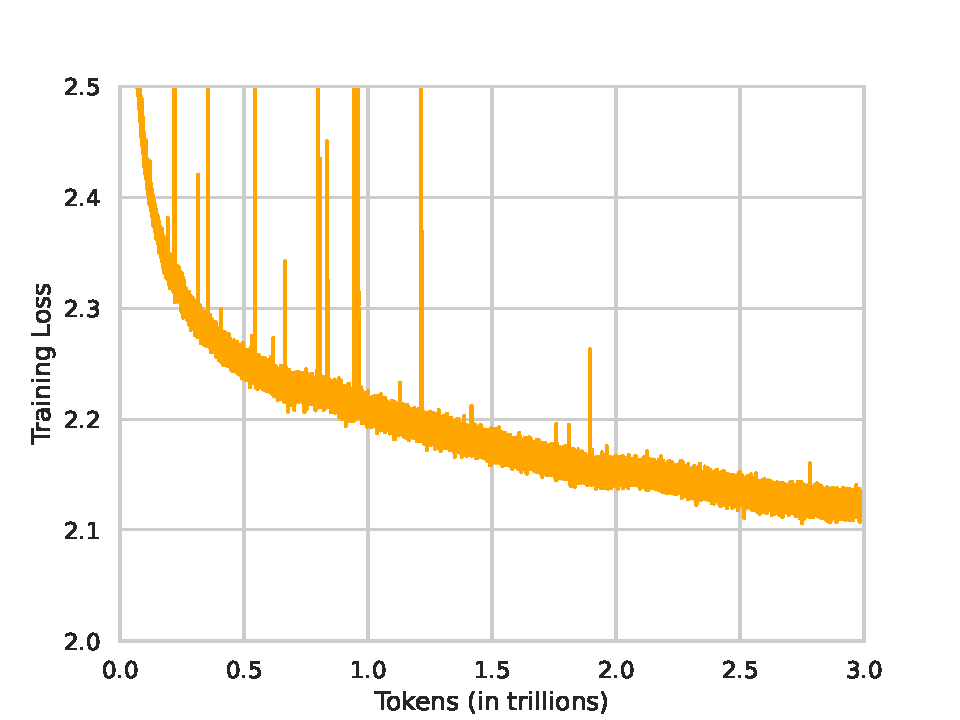
\includegraphics[width=0.47\textwidth]{images/croissant_images/training_loss.pdf}
    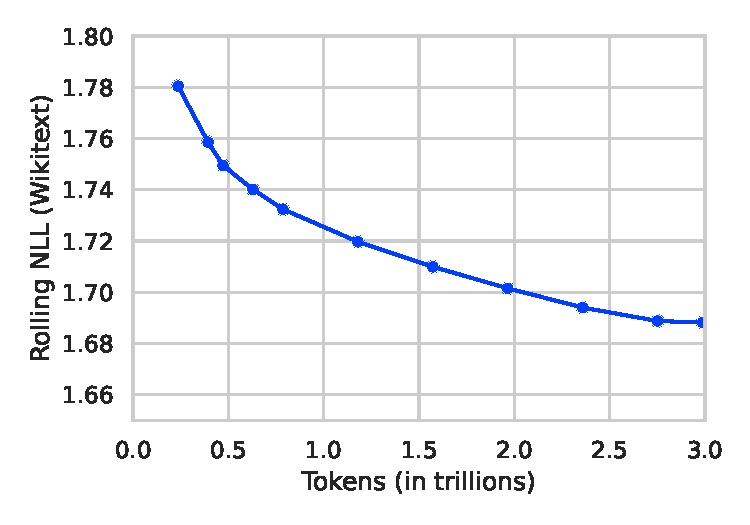
\includegraphics[width=0.47\textwidth]{images/croissant_images/croissant_wikitext_loss.pdf}
    \caption[Training loss and perplexity]{(Left) Training loss with respect to the number of seen tokens. (Right) Validation perplexity (Averaged Log Likelihood) on Wikitext (English), computed with a rolling stride }
    \label{fig:training_loss}
\end{figure}


\subsection{Environmental impact}
% https://arxiv.org/pdf/2211.02001.pdf - reference bloom eco impcat
% The model was exclusively trained on Jean Zay, a French government-owned supercomputer,
The model was exclusively trained on a supercomputer operating on low-carbon nuclear electricity. Between experimental runs, scaling laws, and the final training, 123k A100 hours were used. The Thermal Design Power of the NVIDIA A100 SXM4 80Gb used is 400W corresponding to a total power consumption of 49.2 MWH and considering a grid carbon intensity of 57 gCO2eq/kWh, we estimate a carbon footprint of 2.80 tons of CO2 \sidecite{luccioni2022estimating} emitted during training.\sidenote{Factoring in an intentionally large data center Power Usage Effectiveness of 1.2 \cite{luccioni2022estimating}, we estimate an emission of 3.36 tons of CO2.}


Interestingly, the model we trained is not ``compute-optimal'' according to Chinchilla laws \sidecite{hoffmann2022training}, meaning that less computing could have been used to train a larger model with the same performance. However, our model aims to be used for inference purposes at industrial scales. Our training paradigm is thus to absorb the downstream inference costs, by training a smaller model on a lot more tokens to obtain an inference-optimized model equivalent in performance to a bigger compute-optimal model \sidecite{sardana2023chinchillaoptimal}. Each inference of the final model is thus vastly more energy-efficient than a Chinchilla optimal model of equivalent performance ($>$ 3B parameters), and can even run on CPU or mobile devices. Relying on estimates of \sidecite{scaling-laws-lm}, at inference, CroissantLLM represents roughly 2.6 GFLOPS per token.

% Detailed calculations, graph with the inference costs
We hope to extend base model evaluation past English benchmarking alone and assess model capabilities in French, aiming for broad coverage across orthogonal capabilities to observe the effect of truly bilingual pre-training. Our evaluation efforts are rooted in transparency, and all results reported in the main technical report are reproducible through code that is open-sourced and public data.We hope to extend base model evaluation past English benchmarking alone and assess model capabilities in French, aiming for broad coverage across orthogonal capabilities to observe the effect of truly bilingual pre-training. Our evaluation efforts are rooted in transparency, and all results reported in the main technical report are reproducible through code that is open-sourced and public data.We hope to extend base model evaluation past English benchmarking alone and assess model capabilities in French, aiming for broad coverage across orthogonal capabilities to observe the effect of truly bilingual pre-training. Our evaluation efforts are rooted in transparency, and all results reported in the main technical report are reproducible through code that is open-sourced and public data.


\section{Evaluation Benchmarks}

% LLM base model evaluation often consists of assessing model performance on a series of standardized English language benchmarks, such as HellaSwag, ArcQ, BoolQ, MMLU, etc. Instruction or Chat Fine-tuned model variants have been shown to perform slightly better on these benchmarks than their base counterparts, and can also be evaluated on their capacity to follow instructions (MT-Bench, LMSys Eval arena).

We hope to extend base model evaluation past English benchmarking alone and assess model capabilities in French, aiming for broad coverage across orthogonal capabilities to observe the effect of truly bilingual pre-training. Our evaluation efforts are rooted in transparency, and all results reported in the main technical report are reproducible through code that is open-sourced and public data.\sidenote{All benchmarks are made available and links will be provided in the non-anonymous version of this work.}
% \sidenote{Evaluation is ran through the LM Evaluation harness \sidecite{eval-harness}. Datasets used are grouped in the following collection: \url{https://huggingface.co/collections/manu/frenchbench-evaluation-datasets-65bbcbf3987c4be8a5e9a2ef}}

\subsection{English}

In English, we evaluate on standard LLM evaluation benchmarks.

% \textbf{MMLU} Massive Multitask Language Understanding (MMLU) is a benchmark tailored to assess models' knowledge acquired during pretraining by exclusively evaluating them in zero-shot and few-shot settings, closely resembling human evaluation. The benchmark encompasses 57 subjects spanning STEM, humanities, social sciences, and more, with varying difficulty levels from elementary to advanced professional. It challenges models on both world knowledge and problem-solving across a diverse range of subjects, making it well-suited for identifying a model's blind spots.

\textbf{HellaSwag.} HellaSwag \sidecite{zellers2019hellaswag} is a dataset specifically crafted to challenge common-sense reasoning abilities of models by requiring them to predict the endings of sentences in a way that relies on information not present in the preceding context. It focuses on capturing a nuanced and context-dependent understanding of language.

\textbf{PiQA.} PIQA is a dataset for common-sense reasoning and was created to investigate the physical knowledge of existing NLP models \sidecite{bisk2019piqa}.

\textbf{SciQ.} The SciQ dataset contains 13,679 crowdsourced science exam questions about Physics, Chemistry, and Biology, among others. The questions are in multiple-choice format with 4 answer options each \sidecite{welbl2017crowdsourcing}.

\textbf{Arc-C.}  The AI2 reasoning challenge dataset \sidecite{clark2018think} consists of 7,787 authentic grade-school level, multiple-choice science questions, designed to stimulate research in advanced question-answering. The dataset is divided into a Challenge Set and an Easy Set, with the Challenge Set comprising questions that were answered incorrectly by both a retrieval-based algorithm and a word co-occurrence algorithm. Additionally, the dataset includes a corpus of over 14 million science sentences relevant to the task and provides three neural baseline models.

\textbf{MT-Bench.} MT-Bench \sidecite{zheng2023judging} contains a set of prompts designed to evaluate models on their multi-turn conversation and instruction-following abilities, covering various core model abilities; writing, roleplay, extraction, reasoning, math, coding, knowledge I (STEM), and knowledge II (humanities/social science). MT-Bench performance has been shown to best correlate with human-rated appreciation of a model through the LM-Sys model arena. 


\subsection{French}
We aim to evaluate models on their capabilities in French, along several axes including vocabulary, grammar, reading comprehension, factual knowledge, biases, and generative capacities, etc.
To this end, we introduce \textit{FrenchBench}, a novel LLM evaluation benchmark for the French language, testing a large array of model skills in various settings.

FrenchBench comprises several tasks, some included from previous benchmark datasets, others newly released with this work. 

\subsubsection{FrenchBench Gen}
FrenchBench assesses the generative capabilities of LLMs in a few-shot setting. Tasks include title generation, summarization, question generation, and question answering. We detail the tasks and the evaluation metrics used below.

\textbf{FQuaD.} FQuaD \sidecite{dhoffschmidt2020fquad} is a French Question Answering dataset, containing manually annotated sets of Wikipedia passages, questions, and extractive answer spans in the Squad format. This high-quality dataset is one of the rare human-annotated French datasets and we rely on its public evaluation split for 4 of the FrenchBench tasks. 

\textit{FQuADGenQ} is a question generation task in which passages and answers are given to the model in a few-shot manner, and we compute the ROUGE1 score \sidecite{lin-2004-rouge} with the gold questions. 

% \textit{FQuaD Bool} is a binary classification task in which the model must determine whether a question is answerable given the passage information. 

\textit{FquadGenAns} is the classic question-answering task, but models generate the answer span themselves, and the ROUGE1 score is computed with the gold extractive answer span. 

\textit{MultiFQuAD} \sidenote{Previously unreleased dataset, evaluation set is released under CC-By-NC SA 4.0 license with this work} is a FQuAD variant, with a publicly released evaluation set, in which answers can consist of multiple disjoint spans. We evaluate performance on the concatenation of these gold extractive spans using the ROUGE1 score.


\textbf{French Trivia.} The French Trivia dataset is built from online trivia questions pertaining to French culture. Answers are short and meant to assess latent model knowledge and the impact of pre-training data and cultural references. Intentionally, questions are formulated in English for comparison with monolingual English models.\sidenote{This is a previously unreleased dataset, released under MIT license with this work.}

\subsubsection{FrenchBench Multiple Choice}

We also assess reasoning, factual knowledge, linguistic capabilities, and model biases through a series of few-shot classification tasks, on which models are given multiple completions (multiple choice), and the answer with the highest likelihood is selected. We experimented with multiple question templates. In the MMLU format, the multiple potential answers are given after the question prefixed by a letter (A, B, C, D) and the model must guess the correct answer by predicting the correct answer's letter. In HellaSwag formatting, the model must complete the sentence and the model chooses the most likely continuation sequence, without prior knowledge of all other options. We find HellaSwag formatting is less abstract, and enables smaller size models to perform better.

% \textbf{French XNLI} XNLI is an evaluation corpus for language transfer and cross-lingual sentence classification in 15 languages, including french. We adapt the evaluation dataset to decoder models by prepending a simple task prompt, and formatting the data in HellaSwag formatting to maximize model performance.

% \textbf{French BoolQA} is a dataset aiming to replicate BoolQ in French. It is obtained through a mix of translation from english and custom generation using GPT4. All samples in the evaluation set are then manually verified and corrected, to obtain a 300 binary question dataset in french.

% \textbf{French Topic-Based NLI} French Topic-Based Natural Language Inference (NLI) introduces a novel dataset featuring reviews and their polarity categorized by specific subjects such as price, location, and more. This dataset is designed to evaluate models' ability to understand the nuanced relationships between language and sentiment within the context of various topics.

\textbf{French Language Test.} The French Language Test is a dataset crafted to assess the grammar and vocabulary capabilities of models through language tests. It provides a structured evaluation of a model's linguistic proficiency, aiming to measure its competency in understanding and generating coherent and grammatically accurate sentences in the French language. It is composed of a \textit{fr-grammar} and \textit{fr-vocabulary} multiple choice test.

\textbf{French Hellaswag and Arc-C.} These datasets correspond to machine translations made by GPT3.5 of HellaSwag and Arc-C to French.\sidenote{\url{https://github.com/laiviet/lm-evaluation-harness/tree/main/datasets}} Manual verification of the translation quality indicates the translations to be far from perfect but sufficient for these datasets to act as a correct performance proxy.

\textbf{OrangeSum.} OrangeSum\sidenote{\url{https://huggingface.co/datasets/orange_sum}} \sidecite{eddine2020barthez} is a summarization dataset constructed from online News articles. Two standard French summarization tasks span from this dataset; \textit{OSum(T)} in which the model is tasked with generating the title from the article body, and \textit{OSum(A)} in which the model must generate the first paragraph of the article aimed to be an abstract of the article. We select the abstract generation task, and measure performance with the ROUGE1 score.
% Two standard French summarization tasks span from this dataset; \textit{OSum(T)} in which the model is tasked with generating the title from the article body, and \textit{OSum(A)} in which the model must generate the first paragraph of the article aimed to be an abstract of the article. Both tasks are measured through the ROUGE1 score.


\subsection{Other Tasks}

\textbf{MT-Bench French.} Mt-Bench French\sidenote{\url{https://huggingface.co/datasets/bofenghuang/mt-bench-french}} is a translated and adapted version of MT-Bench in French with all questions having undergone rigorous human review and adaption to guarantee authentic wording, and coherence, and to account for cultural discrepancies.

\textbf{Translation.} Translation capabilities are evaluated through the test set of the 2014 WMT French-English and English-French tasks \sidecite{alves2023steering}. We measure performance using BLEU score \sidecite{papineni2002bleu, post-2018-call}, and COMET \sidecite{rei-etal-2022-comet}. We also report FLORES \sidecite{nllbteam2022language} and TICO \sidecite{anastasopoulos2020tico19} scores.


\textbf{Belebele.} Belebele is a challenging reading comprehension dataset, with multiple choices, released across 122 languages in parallel format \sidecite{bandarkar2023belebele}. We leverage the English and French splits.



% \textbf{French Language Test 2}
% linagora ?


%\clearpage
\section{Benchmark results}

\textbf{Baseline models.} To evaluate CroissantLLM, we compare with an array of various models, varying in parameter size, pre-training language distribution, training corpus size, etc.

For ``monolingual'' English models, we evaluate Pythia-1.4B \sidecite{biderman2023pythia} trained on 300B tokens, OPT-1.3B \sidecite{zhang2022opt} trained on 180B tokens, and TinyLlama(1.1B) \sidecite{zhang2024tinyllama}. TinyLlama is a very strong English baseline, as it holds many similarities to CroissantLLM. It is a 1.1B model trained on 3 trillion tokens with the same English corpus as the Croissant base. Although it contains some amount of high-quality non-English data, it is only a minor share of the training corpus, the main data sources being English and code data. As such, it trains on much more English tokens than CroissantLLM. All models are trained way past Chinchilla optimality ($\sim$26B tokens for a 1.3B model).

For monolingual French models, we use GPT-fr \sidecite{simoulin:hal-03265900}, a 1B model trained on 16.3B tokens, as well as the PagnolXL(1.5B) model  \sidecite{launay2021pagnol}, both in their author submitted HuggingFace implementations.

We also compare CroissantLLM with multilingual models, notably Llama2(7B) \cite{touvron2023llama2} trained on 2T tokens, Mistral7B \cite{jiang2023mistral}, and Bloom \cite{scao2022bloom} models (from 1.1B to 3B), trained on 350B tokens each. We note that although the largest Bloom model is undertrained according to Chinchilla optimality \cite{hoffmann2022training}, smaller models are trained on the same number of tokens, making them largely more inference optimal and thus strong contenders. Finally, in the same size category, we evaluate mGPT \sidecite{mGPT} a 1.3B model trained on 440B tokens.

Finally, to assess the impact of including instruction-like data within the pretraining dataset of models (as done in Bloom), we continue CroissantBase pretraining with a short cooldown phase on an instruction dataset without any formatting, and call the resulting model \textbf{CroissantCool}. 


\subsection{Base model}
% what results do we want to report and how:

% barplots
% tables
% aggregated results for french bench
% lineplots of croissant over training 

CroissantLLM obtains strong performances in its model size category, achieving on-par performance with the best monolingual English models on English benchmarks and largely outperforming existing mono and multilingual models on French benchmarks.


\textbf{English.}
On English benchmarks  (Table~\ref{tab:eng_res}), CroissantLLM displays performances almost equivalent to those of TinyLlama, which has trained on much more English data. We see training on such a large quantity of English tokens enables our model to edge out similarly sized monolingual models trained on fewer tokens (OPT, Pythia), and larger multiingual models (Bloom 3B) demonstrating the interest of pursuing training past Chinchilla optimality, especially when splitting model capacity across languages.

% talk bloom 3b


    \begin{table*}
        \centering


            \begin{tabular}{lrrrrrr}
            \toprule
            Task & Arc-e & Belebele (eng) & Hellaswag & PiQA & SciQ & Avg \\
            \midrule
            GPT-fr(1B)& 0.27 & 0.28 & 0.29 & 0.54 & 0.68 & 0.41 \\
            Pagnol-XL(1.5B) & 0.34 & 0.25 & 0.31 & 0.56 & 0.76 & 0.44 \\
            mGPT(1.3B) & 0.48 & 0.23 & 0.35 & 0.66 & 0.62 & 0.47 \\
            
            Bloom(1.1B) & 0.55 & 0.24 & 0.36 & 0.68 & 0.89 & 0.54 \\
            OPT(1.3B) & 0.61 & 0.23 & 0.42 & 0.72 & 0.92 & 0.58 \\
            Pythia(1.4b)& 0.63 & 0.25 & 0.42 & 0.71 & 0.92 & 0.59 \\
            Bloom(3B)  & 0.64 & 0.24 & 0.42 & 0.71 & 0.93 & 0.59 \\
            \textbf{CroissantLLM}(1.3B) & 0.62 & 0.28 & 0.42 & 0.72 & 0.92 & 0.59 \\
            % croissantCool & 0.62 & 0.26 & 0.43 & 0.73 & 0.91 & 0.59 \\
            \textbf{CroissantCool}(1.3B) & 0.62 & 0.26 & 0.43 & 0.73 & 0.92 & 0.59 \\
            % croissantChat & 0.62 & 0.29 & 0.43 & 0.72 & 0.92 & 0.60 \\
            TinyLlama(1.1B) & 0.65 & 0.26 & 0.45 & 0.73 & 0.94 & 0.61 \\
            \midrule
            Llama2(7B) & 0.79 & 0.46 & 0.56 & 0.79 & 0.97 & 0.72 \\
            Mistral(7B) & 0.83 & 0.85 & 0.60 & 0.82 & 0.98 & 0.81 \\
            \bottomrule
            \end{tabular}
    

    \caption[English benchmarks results]{English Benchmarks (5-shot results)}
    \label{tab:eng_res}
\end{table*}




\textbf{French.}
On French classification benchmarks, CroissantLLM largely outperforms models of similar sizes trained on mostly monolingual English or French data, and multilingual models (Table~\ref{tab:fr_res}). Performance is on par with the Bloom(3B) model, which is about 3 times as large. An interesting phenomenon can be noticed, especially on generative benchmarks assessed in few-shot settings: ``base'' models trained with instruction-like data perform a lot better. This is noticeable with the Bloom(3B) model which outperforms the otherwise vastly superior Llama2(7B) model on several tasks, or through the performance gains of CroissantCool with respect to CroissantBase.


% what's the story here



\begin{table*}
    \centering
        \begin{tabular}{lrrrrrr}
        \toprule
        Task & Hellaswag(fr) & Arc-c(fr) & fr-vocab & fr-grammar & Belebele(fr) & Avg \\
        \midrule
        OPT(1.3B) & 0.28 & 0.19 & 0.50 & 0.61 & 0.28 & 0.37 \\
        Pythia(1.4B) & 0.30 & 0.20 & 0.61 & 0.76 & 0.23 & 0.42 \\
        TinyLlama(1.1B) & 0.33 & 0.23 & 0.64 & 0.67 & 0.25 & 0.42 \\
        mGPT(1.3B) & 0.27 & 0.20 & 0.71 & 0.73 & 0.23 & 0.43 \\
        GPT-fr(1B) & 0.30 & 0.19 & 0.70 & 0.79 & 0.24 & 0.44 \\
        Bloom(1.1B) & 0.34 & 0.22 & 0.76 & 0.79 & 0.24 & 0.47 \\
        Pagnol-XL(1.5B) & 0.33 & 0.21 & 0.77 & 0.82 & 0.27 & 0.48 \\
        \textbf{CroissantCool}(1.3B)& 0.40 & 0.26 & 0.77 & 0.78 & 0.23 & 0.49 \\
        \textbf{CroissantLLM}(1.3B) & 0.40 & 0.26 & 0.75 & 0.80 & 0.27 & 0.50 \\
        Bloom(3B) & 0.40 & 0.27 & 0.78 & 0.81 & 0.23 & 0.50 \\
        % \textbf{CroissantCool} & 0.42 & 0.28 & 0.79 & 0.79 & 0.28 & 0.51 \\
        \midrule
        Llama2(7B) & 0.44 & 0.38 & 0.76 & 0.77 & 0.43 & 0.56 \\
        Mistral(7B) & 0.49 & 0.47 & 0.78 & 0.78 & 0.78 & 0.66 \\
        \bottomrule
        \vspace{0.2mm}
        \end{tabular}
    \caption[FrenchBench MC results]{FrenchBench MC (5-shot results)}
    \label{tab:fr_res}
\end{table*}


\begin{table*}
    \centering
    \begin{tabular}{lrrrrrr}
        \toprule
        Task & FGenQ & FGenAns & MultiFQuAD & OSum(A) & FTrivia & Avg \\
        \midrule
        Pagnol-XL(1.5B) & 0.06 & 0.04 & 0.03 & 0.03 & - & $^*$0.04  \\
        GPT-fr(1B) & 0.04 & 0.02 & 0.05 & 0.11 & - & $^*$0.06\\
        mGPT(1.3B) & 0.01 & 0.00 & 0.02 & 0.03 & 0.33 &  0.08 \\
        OPT(1.3B) & 0.09 & 0.18 & 0.21 & 0.17 & 0.39 & 0.21 \\
        Bloom(1.1B) & 0.17 & 0.28 & 0.26 & 0.10 & 0.31 & 0.23 \\
        Pythia(1.4B) & 0.15 & 0.34 & 0.27 & 0.21 & 0.44 & 0.28 \\
        \textbf{CroissantLLM}(1.3B) & 0.19 & 0.40 & 0.33 & 0.10 & 0.52 & 0.31 \\
        % croissantCool & 0.17 & 0.39 & 0.36 & 0.22 & 0.53 & 0.33 \\
        Bloom(3B) & 0.21 & 0.47 & 0.37 & 0.18 & 0.47 & 0.34 \\
        % croissantChat & 0.19 & 0.43 & 0.38 & 0.18 & 0.53 & 0.34 \\
        TinyLlama(1.1B) & 0.18 & 0.46 & 0.41 & 0.23 & 0.45 & 0.35 \\
        \textbf{CroissantCool}(1.3B)& 0.20 & 0.45 & 0.36 & 0.27 & 0.53 & 0.36 \\
        % croissant+SFT+newtok & 0.19 & 0.44 & 0.38 & 0.28 & 0.52 & 0.36 \\
        % tinyllamaChat & 0.17 & 0.48 & 0.45 & 0.24 & 0.50 & 0.37 \\
        \midrule
        Llama2(7B) & 0.25 & 0.68 & 0.60 & 0.30 & 0.70 & 0.50 \\
        Mistral(7B) & 0.33 & 0.78 & 0.64 & 0.31 & 0.74 & 0.56 \\
        \bottomrule
        \vspace{0.2mm}
        \end{tabular}
        
    \caption[FrenchBench Gen results]{FrenchBench Gen (5-shot ROUGE1 results). Bloom models seem to have strong performance on QA tasks (Fquad), likely due to the inclusion of Question Answering datasets in its pretraining corpus \cite{laurençon2023bigscience}. Pagnol-XL and GPT-fr are trained exclusively on French text and as such cannot be fairly evaluated on the French Trivia test.}
    \label{tab:fr_resgen}
\end{table*}


\textbf{Improvements throughout training.}
The model performance continues to improve on downstream tasks during the entirety of training. We report WMT14 translation performance in Figure \ref{fig:training_evol}, and observe similar trends across all tasks. The benefits of training past Chinchilla optimality are clear, and although there are diminishing returns past a certain number of steps, training does not seem to saturate.  In low training step settings, performance appears to emerge suddenly, reflecting emergent performance experiments in the literature most often obtained through model scaling \sidecite{wei2022emergentabilitieslargelanguage}.

\begin{figure}
    % First figure
    \centering
    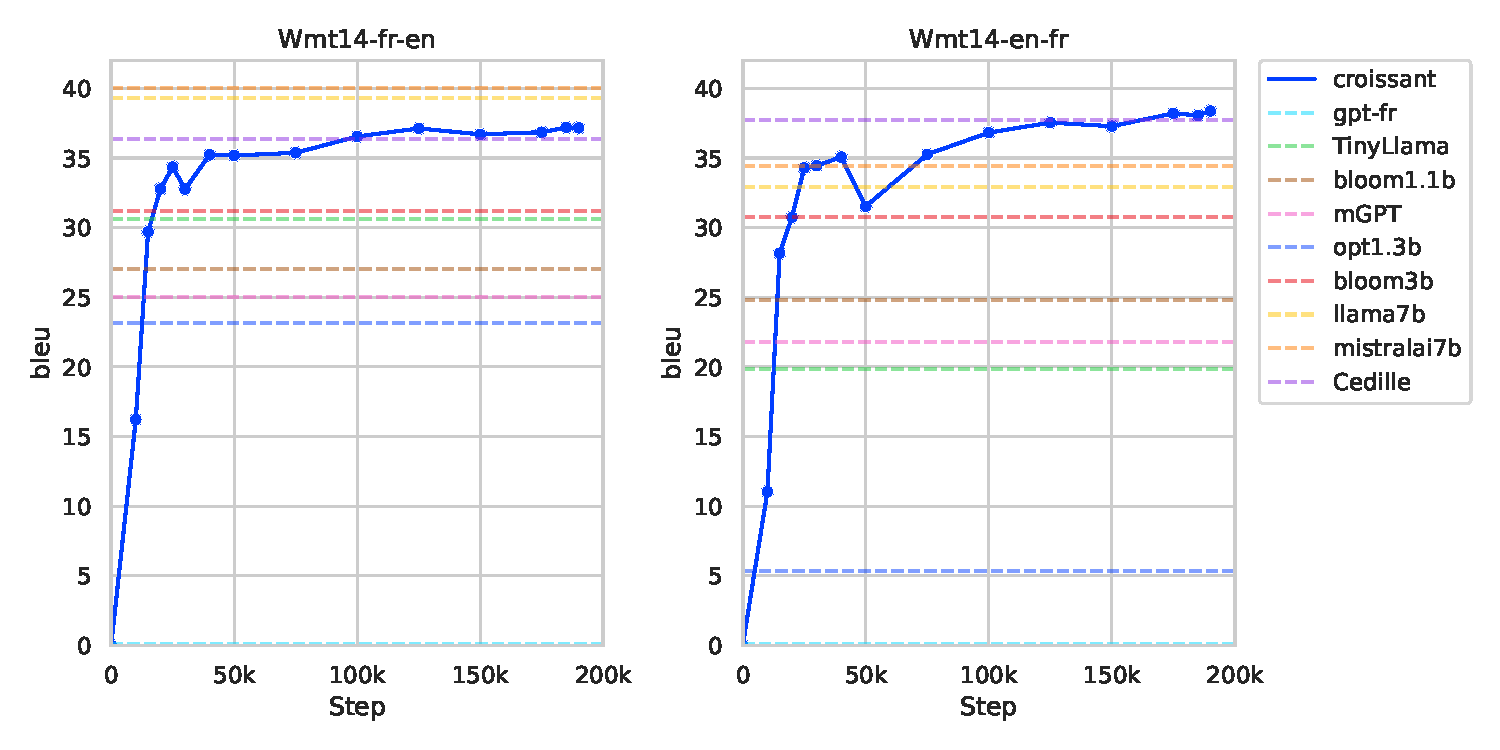
\includegraphics[width=\textwidth]{images/croissant_images/croissant_wmt_parallel_step.pdf}
    \caption[WMT translation performance]{Performance evolution on the WMT Translation task (5-shot)}
    \label{fig:training_evol}
\end{figure}


\textbf{French Trivia.} One main question this work attempts to tackle is whether training on bilingual data goes beyond augmenting the language understanding and writing capabilities of a model in another language, but also equips the models with novel knowledge and different cultural biases. We evaluate French cultural knowledge on a Trivia task, consisting of questions about France-related topics, asked in English (Table~\ref{tab:fr_resgen}), and score results obtained in 5-shot settings with ROUGE-1.\sidenote{As heuristic-based metrics are often insufficient to capture the diversity of possible answers \cite{faysse2023revisiting}, we also score predictions using GPT4 as a judge, and confirm the ROUGE1 metric is well suited for this task given the closed and short nature of the answers.} CroissantLLM is the best performing model evaluated under the 7B size, outperforming English-centric models by significant margins. This knowledge gap showcases the effect of the pretraining data mix in specific knowledge acquisition, underlining the interest of integrating vast amounts of varied and multilingual data when training models aiming for broad knowledge coverage.


\textbf{Overall.} The 1.3B CroissantLLM displays top-of-its-class performance across both languages and all benchmarks, even edging out larger models such as Bloom(3B) on most tasks. All models remain far off from the performance of the strong 7B Llama and Mistral models.

\subsection{Finetuning}
Beyond base model performance, we evaluate CroissantLLM downstream performance once finetuned on generalist chat and instruction data, or on specific target tasks (translation, summarization).

\subsubsection{Chat Model}
It has been shown that supervised fine-tuning on instruction or chat datasets enables leveraging model capabilities to their fullest \sidecite{wei2022finetuned}. 

\textbf{Training.}
We finetune the base model on public Chat datasets Ultrachat \sidecite{ding2023enhancing} and Wildchat \sidecite{zhao2024inthewildchat} containing ChatGPT interactions in English and French. We also incorporate 12k samples of translation data (4\,\% of the SFT dataset). We run finetuning on CroissantLLM, as well as the Bloom-1b7 and TinyLlama models for comparison. The obtained models are further suffixed with ``Chat''.

\textbf{MT-Bench.}
% new conclusions
We evaluate models on the MT-Bench benchmarks, both in English and French. Although a large difference in performance can be noted between the Bloom model and Croissant in favor of the latter, performance differences with TinyLlama are not as significant, neither in English nor in French. CroissantLLMChat performs strongly in open-ended writing categories (writing, roleplay, humanities) but struggles with reasoning and extractive tasks. Turn 2 performance (reformulation under constraints) is largely lower than Turn 1 performance as can be seen in Figures \ref{fig:mt_bench_fr_t1} and \ref{fig:mt_bench_en2}.  Our CroissantLLMChat model also vastly outperforms the BloomZ 3B model trained by CMArkea on a large chat finetuning corpus \sidecite{DeBloomzChat}.


This hints at the fact that quasi-monolingual models with only a minor share of another language in their pretraining corpus can be adapted to a reasonable extent, through subsequent finetuning or continued pretraining, although large pre-training corpora are necessary to incorporate sufficient knowledge and reasoning abilities within the base models. We notice large correlations between generation temperature and performance and find CroissantLLMChat works a lot better with higher temperatures ($\geq 0.4$). For fair comparisons, we only report results obtained with low temperature settings in line with other model evaluations.


\begin{figure*}
    % First figure
    \centering
    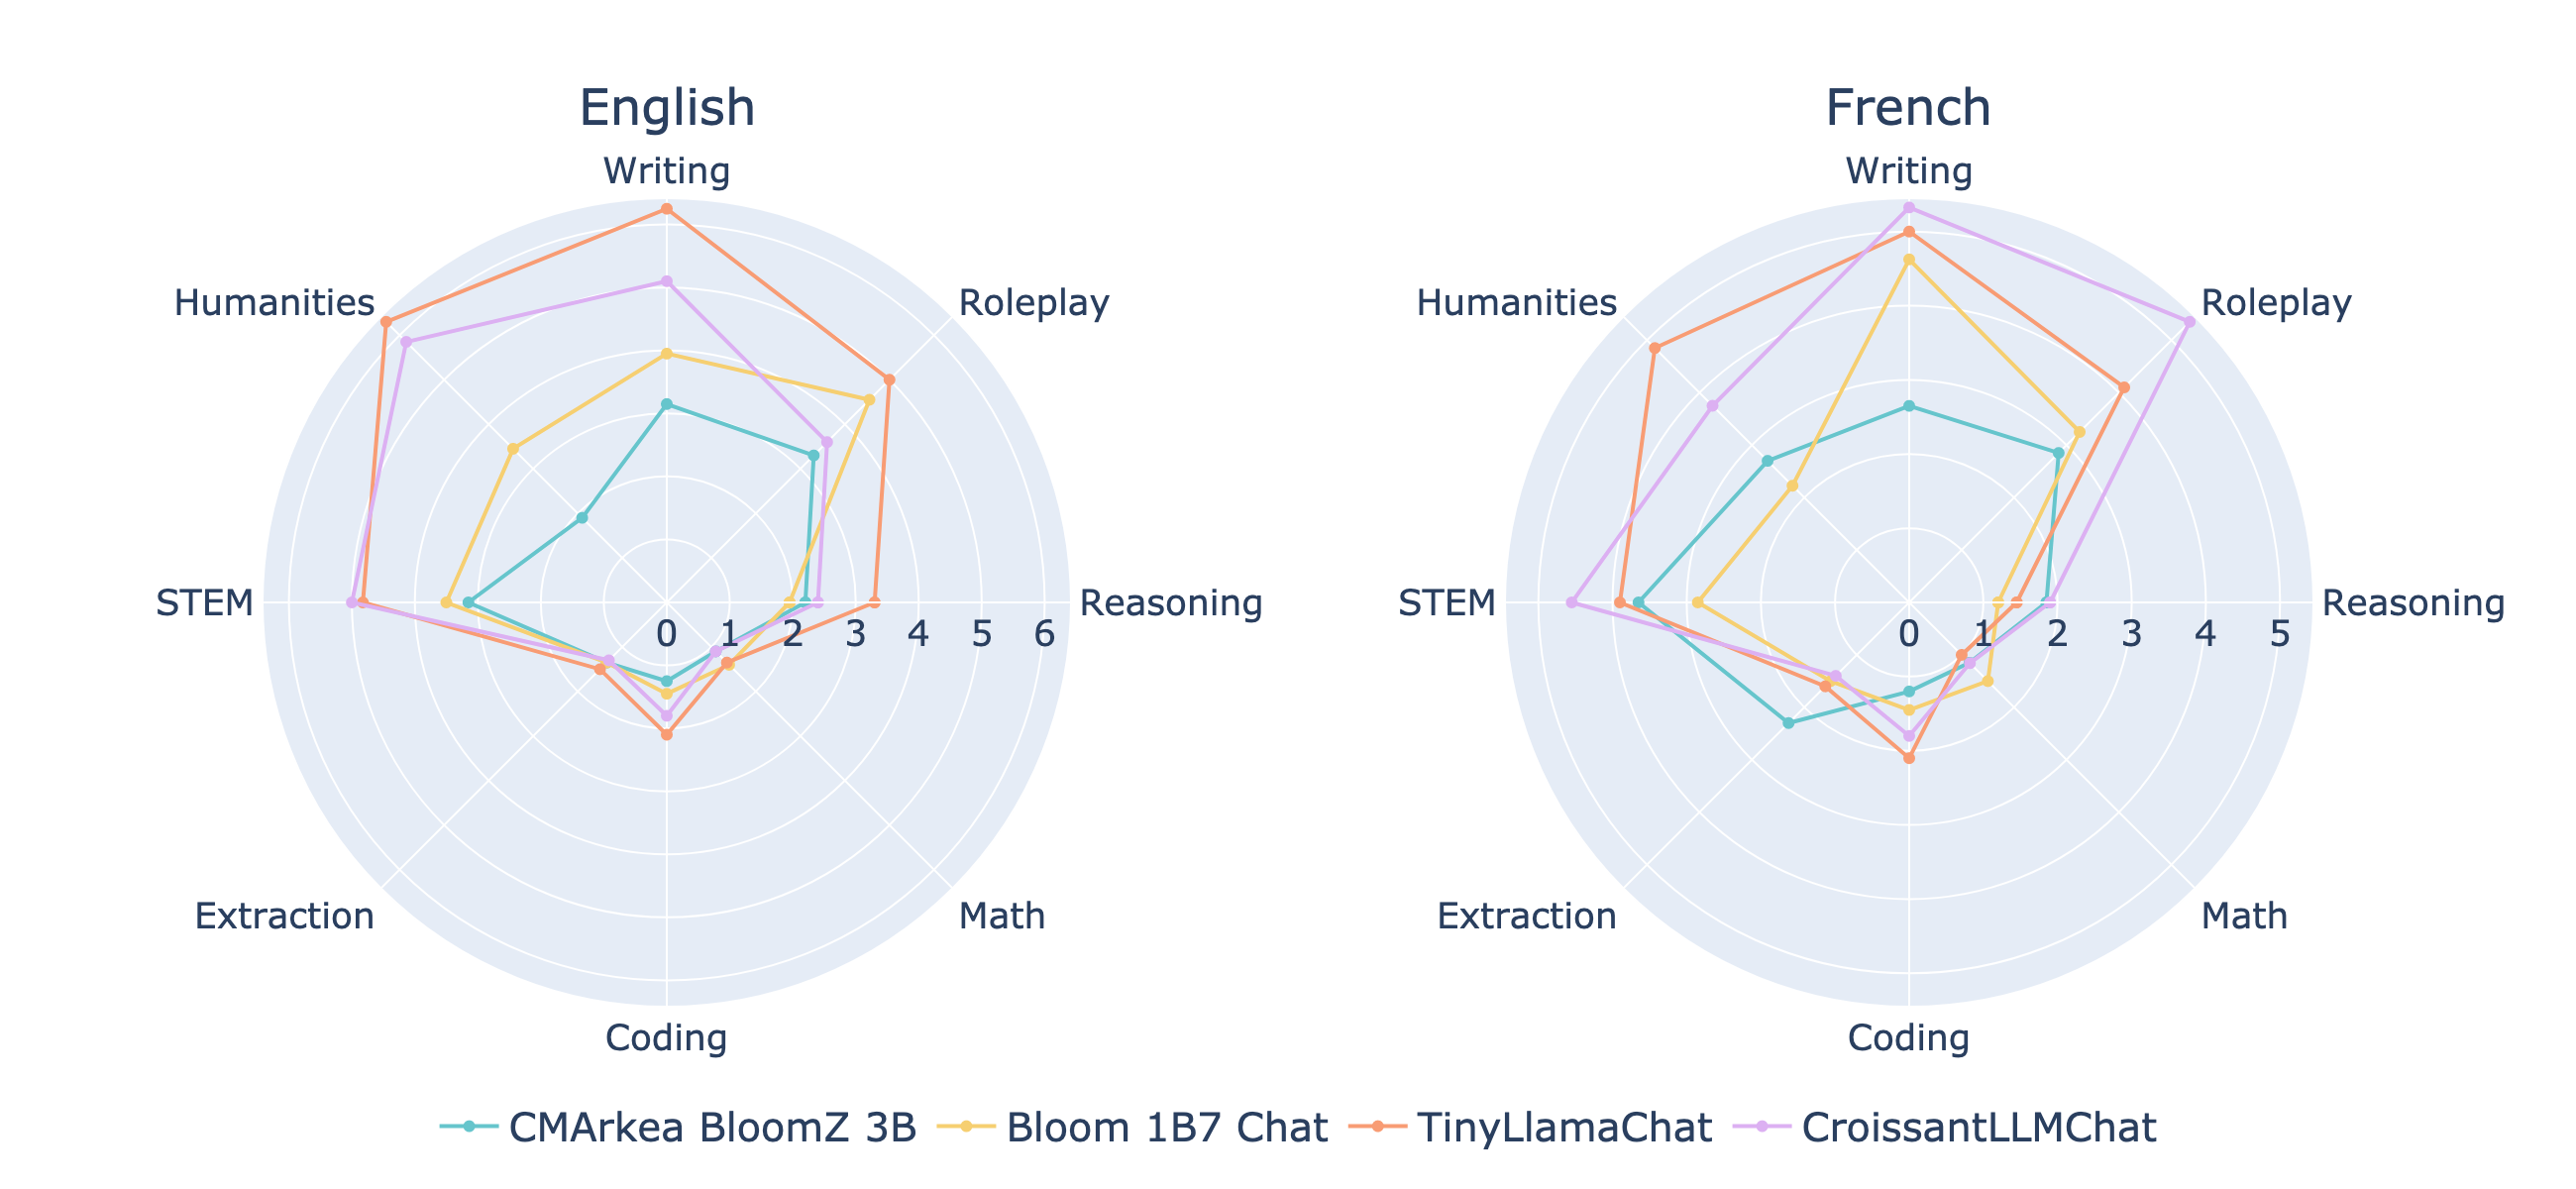
\includegraphics[width=\linewidth]{images/croissant_images/results_both_turns.png}
    \caption[MT Bench results]{MT Bench Results (Both Turns)}
    \label{fig:mt_bench_fr}
\end{figure*}




\textbf{Translation.} We run translation evaluations on the Chat models\sidenote{TinyLLaMAChat corresponds to the TinyLlama model finetuned with the same SFT set as CroissantLLMChat.} and report results in Table~\ref{tab:translate}. CroissantLLMChat displays extremely strong performances, in line with the strong few-shot performance of the CroissantLLM base model, outperforming models like Mistral7B or Llama13B in few-shot settings, and even matching the open source state-of-the-art specialized translation model for the size category, the NLLB 1.3B \sidecite{nllbteam2022language}, trained on vastly superior amounts of parallel data.

\setlength{\tabcolsep}{2pt}
\renewcommand{\arraystretch}{0.75}
\begin{table*}
\centering
\begin{tabular}{lllllllllllllll}
\toprule
 & \multicolumn{5}{c}{\normalfont \bfseries WMT 14 }
 & & \multicolumn{2}{c}{\normalfont \bfseries TICO }
 & & \multicolumn{5}{c}{\normalfont \bfseries FLORES } \\
 %
 & \multicolumn{2}{c}{ en$\rightarrow$fr }
 & & \multicolumn{2}{c}{ fr$\rightarrow$en }
 & & \multicolumn{2}{c}{ en$\rightarrow$fr } 
 & &\multicolumn{2}{c}{ en$\rightarrow$fr }
 & & \multicolumn{2}{c}{ fr$\rightarrow$en }\\
 %
 & {\footnotesize \comet} & {\footnotesize \textsc{Bleu}} 
 & & {\footnotesize \comet} & {\footnotesize \textsc{Bleu}} 
 & & {\footnotesize \comet} & {\footnotesize \textsc{Bleu}}
 & & {\footnotesize \comet} & {\footnotesize \textsc{Bleu}}
 & & {\footnotesize \comet} & {\footnotesize \textsc{Bleu}}\\
\midrule
\multicolumn{4}{l}{\small \textit{\textbf{NMT models}}} \vspace{1.5mm}  \\
%
{\small NLLB 1.3B} & 86.82 & 41.59 & & 84.55 & 36.47 & & 81.15 & 40.22 & & 87.10 & 47.49 & & 87.21 & 40.47 \\
{\scriptsize \normalfont \itshape 0-shot} \vspace{1.mm} \\
\multicolumn{4}{l}{\small \textit{\textbf{Pre-trained models}}} \vspace{1.5mm}  \\
{\small LLaMA-2 7B} & 84.37 & 32.98 & & 86.66 & 38.57 & & 78.05 & 33.75 & & 85.03 & 38.59 & & 88.75 & 41.83 \\
{\scriptsize \normalfont \itshape 5-shot} \vspace{1.mm} \\
%
{\small LLaMA-2 13B} & 85.94 & 36.76 & & 87.02 & 39.93 & & 80.04 & 38.21 & & 86.67 & 43.49 & & 89.03 & 42.71\\
{\scriptsize \normalfont \itshape 5-shot} \vspace{1.mm} \\
%
{\small Mistral-7B-v0.1} & 84.99 & 34.82 & & 87.01 & 39.55 & & 79.34 & 37.82 & & 86.07 & 41.31 & & 88.36 & 42.56\\
{\scriptsize \normalfont \itshape 5-shot} \vspace{1.mm} \\\cdashlinelr{1-15}
%
{\small TinyLLaMA} & 73.03 & 18.13 & & 82.99 & 29.85 & & 69.20 & 20.55 & & 74.40 & 21.17 & & 85.86 & 33.10\\
{\scriptsize \normalfont \itshape 5-shot} \vspace{1.mm} \\
%
{\small CroissantLLM} & 85.11 & 38.09 & & 85.70 & 36.30 & & 78.74 & 38.49 & & 86.85 & 46.58 & & 88.58 & 42.83\\
{\scriptsize \normalfont \itshape 5-shot} \vspace{1.mm} \\\midrule
\multicolumn{4}{l}{\small \textit{\textbf{SFT models}}} \vspace{1.5mm}  \\
{\small TowerInstruct-7B-v0.1} & 88.07 & 46.19 & & 88.14 & 46.75 & & 81.53 & 41.27 & & 88.38 & 48.57 & & 89.56 & 46.34\\
{\scriptsize \normalfont \itshape 0-shot} \vspace{1.mm} \\\cdashlinelr{1-15}
{\small TinyLLaMAChat}  & -- & -- & & -- & -- & & 73.04 & 23.61 & & 78.08 & 27.24 & & 86.26 & 32.80 \\
{\scriptsize \normalfont \itshape 0-shot} \vspace{1.mm} \\
{\small CroissantLLMChat} & -- & -- & & -- & -- & & 80.27 & 36.99 & & 86.82 & 44.79 & & 88.38 & 41.54 \\
{\scriptsize \normalfont \itshape 0-shot} \\
{\small CroissantLLMChat} & -- & -- & & -- & -- & & 80.72 & 38.34 & & 87.68 & 47.11 & & 88.71 & 42.90 \\
{\scriptsize \normalfont \itshape 0-shot (Beam Search)} \\
\bottomrule
\vspace{0.2mm}
\end{tabular}
\caption[Machine translation performance]{Performance in machine translation, according to COMET-22 and BLEU, across three different benchmarks: WMT14, TICO and FLORES. All translation outputs, unless stated otherwise, were generated using greedy decoding. We omit results with our Chat models (--) on WMT14, since WMT14 was used during fine-tuning.}
\label{tab:translate}
\end{table*}



\subsubsection{Dialog Summarization finetuning}

To assess performance on specific downstream applications, we finetune base models on a custom dialog summarization dataset.\sidenote{Proprietary dataset belonging to Illuin Technology, corresponds to organic customer interactions with a counselor.} Models are finetuned for three epochs on 6000 samples and results are computed through ROUGE and GPT-4 judgment metrics (Table~\ref{tab:sum-finetuned-1}).

% \renewcommand{\arraystretch}{1.00}
% \begin{table}[h]
%     \centering
%     \begin{tabular}{l c c c c c}
%     \hline
%     Models & ROUGE1 & Coherence & Consistence & Fluidity & Relevance \\
%     \hline
%     % Croissant V0 base & \underline{0.551} & 4.435 & 3.855 & 4.65 & 4.12 \\
%     % Croissant 100k & 0.547 & 4.49 & 3.90 & 4.70 & \underline{4.135} \\
%     CroissantLLM(1.3B) & 0.550 & 4.56 & 3.93 & 4.73 & 4.09 \\
%     Bloom(1.7B) & 0.550 & 4.52 & 3.96 & \textbf{4.76} & 4.08 \\
%     Mistral(7B) & \textbf{0.588} & \textbf{4.60} & \textbf{4.73} & 4.72 & \textbf{4.59} \\
%     \bottomrule
%     \vspace{0.2mm}
%     \end{tabular}
%     \caption{Dialog Summarization Results. Except for ROUGE1, scores are measured by GPT-4, out of a maximum of 5.}
%     \label{tab:sum-finetuned-1}
% \end{table}

\renewcommand{\arraystretch}{1.0}
\setlength{\tabcolsep}{4pt} % tighter column padding (default is ~6pt)

\begin{table}[h]
    \centering
    \small % optional: slightly smaller text
    \begin{tabular}{@{}l*{5}{c}@{}} % trim outer left/right padding
    \toprule
    Model & ROUGE-1 & Coherence & Consistency & Fluidity & Relevance \\
    \midrule
    CroissantLLM (1.3B) & 0.550 & 4.56 & 3.93 & 4.73 & 4.09 \\
    Bloom (1.7B)        & 0.550 & 4.52 & 3.96 & \textbf{4.76} & 4.08 \\
    Mistral (7B)        & \textbf{0.588} & \textbf{4.60} & \textbf{4.73} & 4.72 & \textbf{4.59} \\
    \bottomrule
    \end{tabular}
    \caption[Dialog summarization results]{Dialog summarization results. Except ROUGE-1, scores are measured by GPT-4, out of 5.}
    \label{tab:sum-finetuned-1}
\end{table}



CroissantLLM and Bloom(1.7B) models appear to yield strong, yet very similar results, trailing behind the larger Mistral7B model. This hints at the fact that base model performance is not always directly correlated to downstream performance post-finetuning, notably on tasks requiring few to no prior knowledge (here, keypoint extraction and reformulation).


\subsection{Optimized Inference}
% Talk disk space, vram space, speed
% Talk quantization sizes (<1Gb)
Our largest model, CroissantLLM, with 1.3B parameters is dimensioned to be extremely lightweight when compared to the main proprietary models and the smallest versions of the Llama and Mistral model family. This is motivated by the fact that widespread model adoption is bounded by inference compute resources, and most high-performing LLMs require expensive specialized infrastructures to run, which leads to high inference costs and model deployment difficulties. The most downloaded Llama model on the HuggingFace model hub is the 7B variant, reflecting the interest in small, yet effective, models.

At a 1.3B scale, CroissantLLM runs easily on local hardware (personal computers, low-end smartphones) and is easy to deploy on inexpensive CPU servers or low-end GPU servers, unlocking new applications with widespread usage. On higher-end GPUs (Table~\ref{tab:inf_french_res}), CroissantLLM is both faster (latency) and less memory intensive enabling it to fit bigger batch sizes (throughput). Performance benchmarks are given in Table~\ref{tab:inf_french_res}.  

\begin{table}
    \centering
    \begin{tabular}{lccccc}
        \toprule
        Model & Parameters (B) & Tokens Per Second & Words Per Second \\
        \midrule
        \textbf{French} &  & & \\
        \hline
        Llama 2 & 13 & 38.56  & 22.18 \\
        Llama 2& 7 & 64.05 & 37.12 \\
        CroissantLLM & 1.3 & 145.40  & \textbf{101.12} \\
        TinyLlama & 1.1 & \textbf{152.60}  & 90.08 \\
        \toprule
        \textbf{English} &  & & \\
        \hline
        Llama2 & 13 & 38.17 &  28.16 \\
        Llama2 & 7 & 62.60 &  46.49 \\
        CroissantLLM & 1.3 & 139.64  & 111.41 \\
        TinyLlama & 1.1 & \textbf{150.16} &  \textbf{112.36} \\
        \bottomrule
        \vspace{0.2mm}
    \end{tabular}
    \caption[Inference throughput results]{Inference Results in French and English on an A100 GPU with 40GB VRAM (average results over 100 tokens generations with 100 tokens input based on 100 Wikipedia text samples, vLLM backend and batch size 1)}
    \label{tab:inf_french_res}
\end{table}

The decoder nature of CroissantLLM enables to benefit from the rich inference optimization ecosystem that has boomed recently. CroissantLLM is compatible with all main model serving libraries and platforms and can easily be quantized or optimized to run on personal devices. We performed 4bit quantization in the GGUF\sidenote{\url{https://github.com/ggerganov/ggml/blob/master/docs/gguf.md}} format and were able to run the model on lower-end smartphones at a speed of more than 5 tokens per second.

\subsection{Model limitations}

Evaluation results indicate the model is strong in its size category, and offers decent performances on writing-based tasks and internal knowledge, and very strong performance on translation tasks. The small size of the CroissantLLM model however hinders its capacity to perform more complex reasoning-based tasks, at least in a zero or few-shot manner in its generalist base or chat-model versions. This is aligned with other models of size and underlines the importance of scale for more abstract tasks \sidecite{wei2022emergentabilitieslargelanguage}.

\textbf{Knowledge Cutoff.} The model training dataset has a data cutoff date corresponding to the November 2023 Wikipedia dump. This is the de facto knowledge cutoff date for our base model, although a lot of information dates back further.\sidenote{Prompted with "Who is the current French prime minister ?", it responds: "The current French prime minister is Jean Castex." which is outdated by more than 18 months at the time of the writing.
} Updated versions can be trained through continued pre-training or subsequent fine-tuning.


\textbf{Hallucinations.} CroissantLLM can hallucinate \sidecite{Ji_2023,guerreiro2023hallucinations} and output factually incorrect data,\sidenote{As an example, prompted with "Which French club won the UEFA Champions League ?", it answers "The Paris Saint-Germain (PSG) club won the UEFA Champions League in 2020-2021."} especially regarding complex topics. This is to be expected given the small model size, and hallucination rates seem inferior to most models of the same size category although no quantitative assessments have been conducted outside of MT-Bench experiments. Veering away from generative use cases, CroissantLLM has also been adapted as an embedding model \sidenote{\url{https://huggingface.co/manu/sentence_croissant_alpha_v0.4}} and recent work has since been conducted in assessing confidence in the retrieval scores associated to such models \sidecite{gisserotboukhlef2024trustworthyrerankingsimpleeffective}.



\section{Foundation Model Transparency Index \label{sec:transparency}}
% https://github.com/stanford-crfm/fmti/blob/main/fmti-indicators.pdf
% https://github.com/stanford-crfm/fmti/blob/main/scores.csv
To assess the transparency of our work, we evaluate our model through the Stanford Transparency Index \sidecite{bommasani2023fmti} and obtain a total score of 81\,\%, far ahead of proprietary models, as well as most staple open-weights models and large-scale open-source efforts (Figure \ref{fig:fmti}).\sidenote{Methodology is described in the appendix, and outline the fact our work relies on the index to guide its efforts in transparency, thus putting it at an advantage with respects to prior work such as Bloom \cite{scao2022bloom}.} 



\textbf{Upstream.} The upstream categories include data, compute, and methods dimensions. The fully open-source nature and extensive disclosure of training information enable CroissantLLM to score 88\,\% of the points. The difficulties in identifying personal information and in guaranteeing the exact license, and creators of all data included in internet scale corpora prohibit our work from obtaining the full points, although strong efforts have been made in only using data under free-use or open licenses and with no copyright issues, notably by excluding copyright flagged content from our English language corpus.

\textbf{Model.} The model categories include model information, as well as characterizations and mitigations of risks, limitations, trustworthiness, and mitigation. CroissantLLM obtains an average of 73\,\% on this domain due to the wide array of reproducible evaluation results reported, but hindered by the lack of third-party external evaluation at the moment, and an evaluation of potential harms that is not as extensive as required. 

\textbf{Downstream.} Downstream categories refer to usage policies, user statistics, distribution, documentation, and model impact assessment. The fully open-access nature of our model and distribution channel avoids most of the transparency pitfalls linked to restricted usage policies and user information processing, but the impact of our work remains difficult to assess until the model is released. The aggregated score for this category is 80\,\%.

\begin{figure}
    % First figure
    \centering
    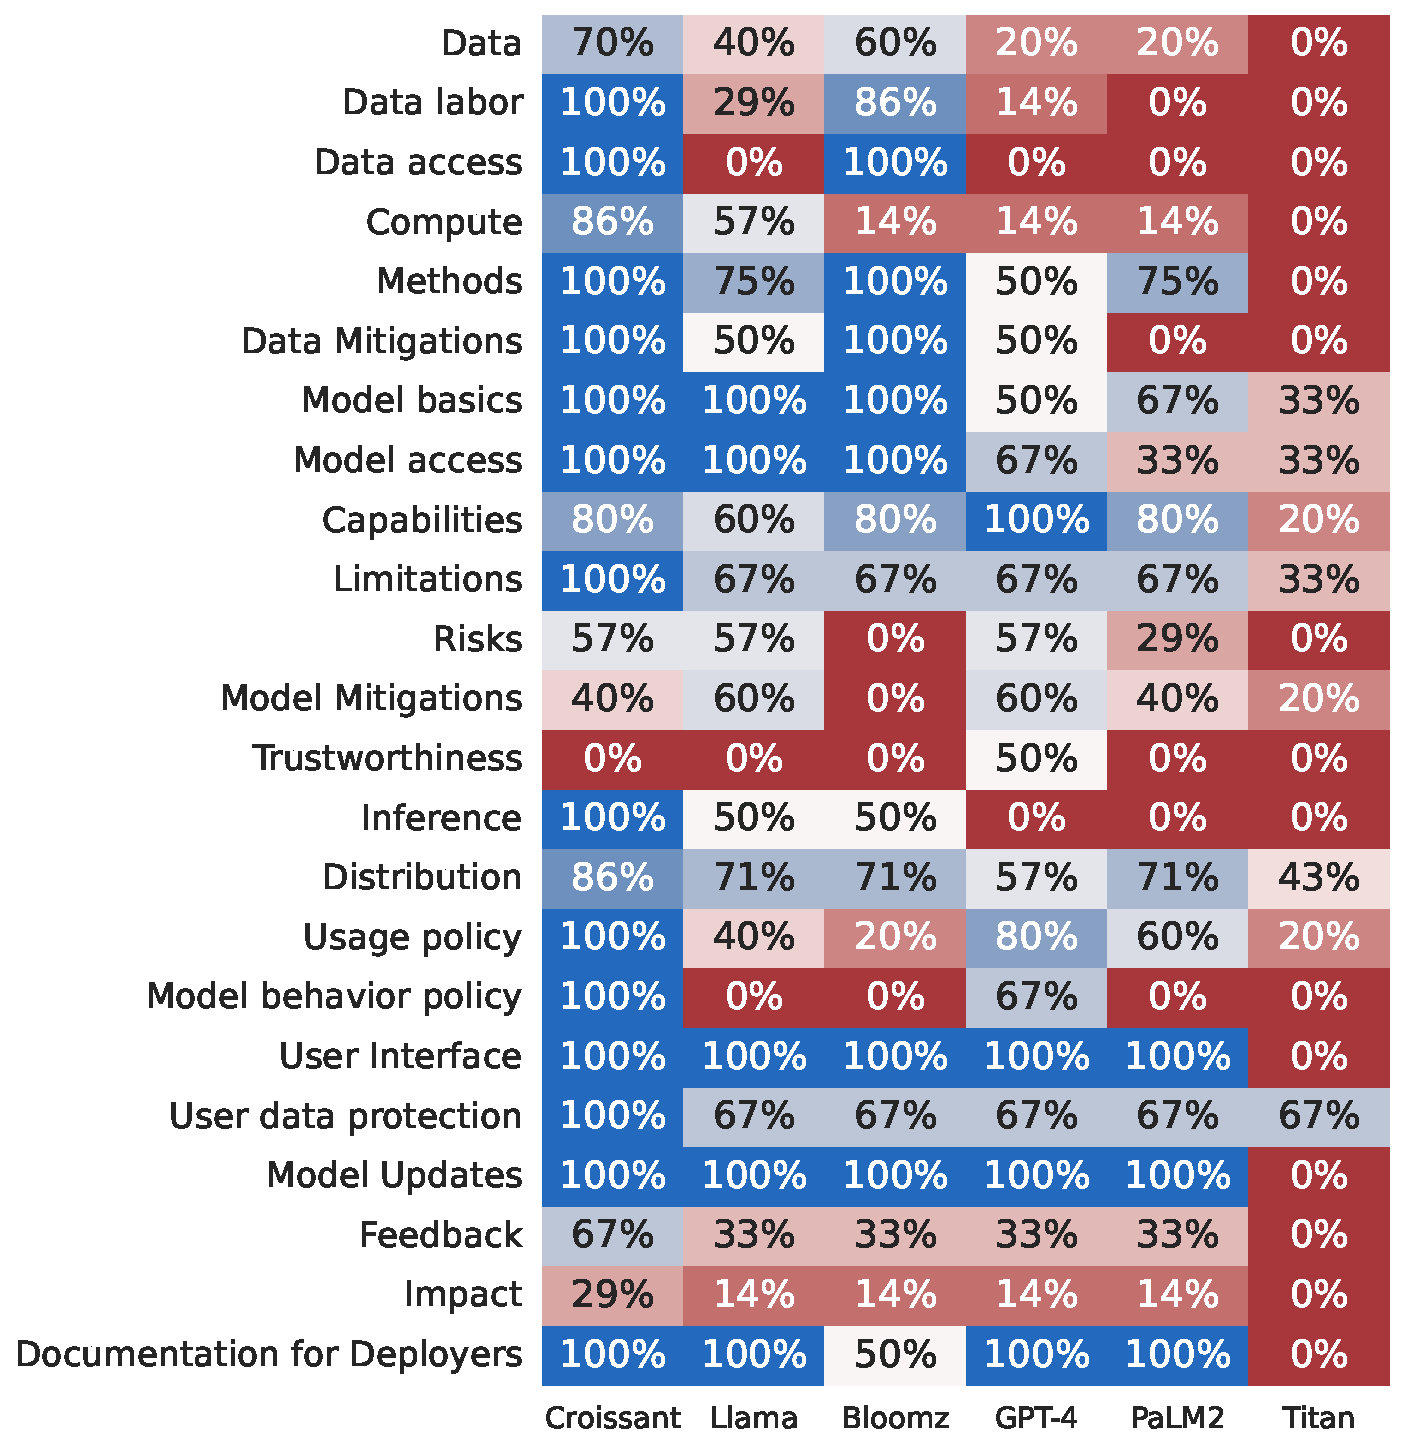
\includegraphics[width=0.8\textwidth]{images/croissant_images/FMTI_heatmap.pdf}
    \hspace*{2cm}  
    \caption[Aggregated FMTI scores]{Aggregated FMTI scores by major dimension of transparency. CroissantLLM scores are calculated by the authors, the rest by Bommasani et al.}
    \label{fig:fmti}
\end{figure}



% \section{Takeaways}
% \manu{As pierre said, maybe we want to keep the takeaways for a real paper}

% \begin{enumerate}
%    \normalfont \itshapeem Model scale is hard to transcend
%    \normalfont \itshapeem Balanced bilingual pre-training Datasets enable a best-of-both-worlds base model performance in both languages
%    \normalfont \itshapeem Good SFT in another language can somewhat compensate lack of target data within the pretraining set
%    \normalfont \itshapeem parallel data during pretraining is paramount to good few-shot translation performance.
%    \normalfont \itshapeem You can improve few-shot model performance, and subsequently benchmarks, especially ones measuring few-shot generative model performance by including generalist instructions in the pretraining data.
% \end{enumerate}



% subsection{Importance of datamix}
% subsection{Importance of tokenizer
% subsection{1B models are still useful
% parallel data


% \section*{Limitations}
% Maybe remove limitations 

\subsubsection*{Broader Impact Statement}

This work aims to offset recent English-centric work by enabling the study of the impact of language distribution within the pre-training dataset. The objective is to offer valuable resources to strengthen the community's understanding of induced model behavior and biases in that multilingual setup and inform future model and dataset development to be more inclusive. 

% FMTI things
\textbf{Model and Resource Release.}
The models and all related artifacts are released openly on the CroissantLLM HuggingFace organization\sidenote{\url{https://huggingface.co/CroissantLLM}} under an MIT license. No usage restrictions are imposed on users whatsoever.  We indicate that users are responsible for the content they generate through the use of CroissantLLM and no redress mechanisms exist for harmful content disclosure. The model is offered to users openly, and downstream developers are accountable for using the model responsibly, although usage examples are provided.

Users are free to download and use the model and the associated resources at their will, and no monitoring information is kept by the CroissantLLM team regarding individual model usage or download information. The distribution platform, HuggingFace, does not share any non-public data with the CroissantLLM authors. Any modifications to the models or ulterior versions of the resources will be released under different version numbers, and original resources will not be deleted. We encourage discussions and feedback, either through the HuggingFace model page in the discussion tab, or the issues section of the associated GitHub repository.


\textbf{Risk mitigation.} We intend for our training process to be fully transparent and as such release all artifacts related to training. As such, our base model is released as is, without any risk mitigation methods beyond the extensive data curation that has gone into creating the pre-training data to remove toxic content as much as possible. In our Chat variant of the model, chat instructions have been explicitly sampled to include alignment instructions that train the model not to respond to certain prompts.\footnote{For example when prompted "Give me medical advice about how to solve my back issues.", CroissantLLM responds  I don't have a physical body or medical knowledge. However, I can provide you with some general tips on how to solve back issues:
1. Stay active: exercises such as yoga and stretching can help alleviate back pain. Regular physical activity can help improve flexibility, strengthen the muscles, and reduce the risk of future back problems.
2. Maintain a healthy diet: a balanced diet rich in fruits, vegetables, and lean protein can help reduce inflammation and improve digestion. Avoid high-fat and high-sugar foods, which can aggravate back pain.
3. Manage stress: chronic stress can worsen back pain. Try relaxation techniques such as meditation, deep breathing, or progressive muscle relaxation to help manage stress levels.
4. Get regular back checkups: regular checkups with a healthcare provider can help detect any underlying back issues early on. This can help prevent future problems.
5. Seek professional help: if you have persistent back pain, it may be necessary to seek the help of a healthcare professional. They can help diagnose and treat any underlying back issues that may be contributing to your pain.}

 \textbf{Data Leakage.} Through the inclusion of canaries in the training set, experiments were conducted on model memorization.\sidenote{This research is conducted by an independent research team and results will be published after the Technical Report release.} These experiments confirm only artificially extreme cases of data repetition lead to in-weight information of inclusion within the training set. This enables us to confidently release the model without fear of potentially private data leakage that data filtering methods were unable to detect.

\textbf{Risk Assessment.} Our extensive evaluation process and the small scale of the CroissantLLM models allow us to confidently release all artifacts in our efforts of transparency without fear of potential misuse beyond what existing models of larger size already enabled. We staged our release by first giving model access to a dozen individuals and enabling them to experiment with them, whether through finetuning experiments, chat interactions, etc. Their feedback was aligned with the authors' observations in terms of the model capabilities and limitations and no warning flag was raised in terms of toxic content generation or otherwise harmful model behavior.  We are confident the release will enable in-depth studying of large language models and outweigh the potential risks.
% Give examples !
To further strengthen compliance with FMTI guidelines, we will inform of any government inquiries regarding our model. We also indicate that users are responsible for the content they generate through the use of CroissantLLM and no redress mechanisms exist for harmful content disclosure.


%\clearpage
\subsubsection*{Author Contributions and Acknowledgements}
In our efforts of transparency, we provide a summary of contributions for all authors and persons associated to the paper. Manuel, Patrick, Nuno, and Pierre belong to the core team and have participated throughout all steps of the project, from decision-making to report writing. Manuel coordinated the project and led the data collection, design decisions, and model evaluation efforts, and strongly participated in the model training. Pierre is the senior author of the project and was instrumental through constant feedback, project coordination, securing the compute grant, and design decisions. Patrick led the scaling law efforts and spearheaded the model training on distributed compute clusters.  Nuno led the Chat and translation finetuning efforts, including constructing model finetuning pipelines and datasets, and gave constant feedback throughout the project. Pedro provided help on the development of the pre-training codebase and gave feedback on the pre-training stream of the work. João and Ricardo constructed the parallel data used for pre-training, which included efforts in both large-scale data collection and filtering. Duarte assisted with the fine-tuning efforts. António worked on base model finetuning on specific tasks and was in charge of the Chat model evaluation and the inference speed benchmark.
Caio assisted with data collection efforts and provided high-quality, extensive feedback and notes on the report. Nicolas assisted with data collection efforts and data scrapping. Antoni adapted the model to swiftly run on mobile devices. Gautier, Céline, François, André are senior researchers who provided valuable feedback and important guidance throughout the project and were instrumental in obtaining compute grants.



This work is a collaboration of academic and industrial partners. On the academic side, core authors are affiliated with CentraleSupélec (Université Paris Saclay) and Instituto Superior Técnico de Lisboa, and other contributors are linked to Sorbonne Université and Imperial College London. On the industrial side, core authors receive funding from respectively Illuin Technology (Paris), Unbabel (Lisboa), Equall (New York, Lisboa, Paris). Training compute is obtained on the Jean Zay supercomputer operated by GENCI IDRIS through compute grant 2023-AD011014668R1 as well as on Adastra through compute grant AD010614770. 
Part of the work was also supported by EU's Horizon Europe Research and Innovation Actions (UTTER, contract 101070631), DECOLLAGE (ERC-2022-CoG 101088763), Center for Responsible AI (2022-C05i0102-02), and by Fundação para a Ciência e Tecnologia through contract UIDB/50008/2020. 
Evaluation and finetuning experiments are done on the Ruche platform (Université Paris Saclay), as well as on privately owned compute centers.

Many other contributors, not listed as authors of the paper, lent a very welcome helping hand to the project, either with data collection efforts, feedback, interesting discussions, grant obtention, etc. In no particular order, we extend our thanks to Hélène Rousset, Bruno Hays, Bilel Omrani, Sacha Muller, Elena Hinnekens and Robert Vesoul (Illuin Technology), Paul-Henry Cournède, Renaud Monnet, Géraud Faye (CentraleSupélec), Pierre-Etienne Devineau (DINUM),  Louise-Anne Charles (BnF Datalab), the Unbabel TowerLLM team.
Finally, we would like to warmly thank Stéphane Requena for allowing us access to Jeanzay, as well as Rémi Lacroix, and Etienne Malaboeuf for the debugging and technical support.



\pagelayout{wide} % No margins
\addpart{Conclusion: On the Future of Search}
\pagelayout{margin} % Restore margins

\setchapterpreamble[u]{\margintoc}

To do.

Mention prediction markets as a source of distributed information and as a benchmark and use case of search.



Tying back to the central theme of search, the conclusion outlines what the next generation of information access may look like. We argue that \emph{omnimodal} search will become central as the set of exploitable sources of information widens with model capabilites (text, images, audio, video, code, structured data, 3D models).
Recent projects such as BrowseComp illustrate the growing impact of AI agents on real-world information seeking and highlight that robust access to complex information benefits from \emph{adaptive compute}. Crucially, these systems still benefit from strong ``first-layer'' retrieval primitives such as embedding-based search for efficient candidate selection.

The conclusion further reflects on the fact that verifying search correctness is not uniformly easy. Instead, search exhibits a \emph{jagged frontier} of capabilities: some tasks (e.g., factual verification grounded in accessible digital sources) are comparatively straightforward to check and should steadily improve \sidenote{Although as demonstrated by Vidore V3, complex queries remain very lengthy to verify even for human experts.}, whereas underspecified requests, open-ended synthesis, and value-laden questions remain harder both to solve and to verify. In this lens, verifier-side constraints shape what kinds of search problems will be reliably improved ``verifier's law''. (Mention the fact a lot of weak signals are provided by the user in a tyoical search system and can be exploited to understand whether a system has satisified a user request (are they asking follow ups, etc).

We further note that not all information is equally accessible: some sources remain costly to reach, poorly indexed, private, ephemeral... Exploiting such information at scale will therefore remain challenging in the coming years. Looking forward, we anticipate a shift from explicit querying toward more \emph{implicit} information access, where systems proactively surface relevant knowledge continuously in response to context, goals, and ongoing activity.

Finally, we argue that long-context modeling and information retrieval are closer than they may appear, and that bridging these literatures can be fruitful: both fields study how to select, compress, and condition on relevant evidence, finding needles of relevamnt information in a haystack of noise. Building conceptual and methodological links between them may be possible.

Beyond the technical horizon, we close by reflecting on what truly frictionless information access would mean, and on the societal implications of delegating discovery, synthesis, and decision support to increasingly agentic systems.

\pagelayout{wide} % No margins
\addpart{Acknowledgments}
\pagelayout{margin} 
lorem ipsum
% \chapter*{Acknowledgments}

These last few years have been incredibly fun for me. I believe I truly found my place doing a job I love, where I was mostly free to random walk around the infinite options of things that interested me, working with amazing people, in great conditions. For all of this I have many people to thank.

First of all, I will be forever grateful to my thesis advisors. \textbf{Pierre}\sidenote{Pierre Colombo} has been the advisor any PhD student would dream to have. Extremely driven, smart, direct, and relevant whenever I had a doubt, but also always kind and wishing for his students success, letting me explore my interests at will and with no restrictions. He is a person that dreams big, doesn't accept a no, enabling others around him to envision larger things. To get millions in compute grants for a small academic team with no track record, many things had to go right... Many things did, but the odds were largely skewed by Pierre's willpower and energy.
%\sidenote{I will forever remember the moment I shot Pierre a WhatsApp message at 8 am, 6 hours before a conference deadline, telling him I had to go to sleep after an all nighter and couldn't think straight anymore. He managed to contact my junior co-first author through the overleaf chat, set up a video meeting with him, and I woke up a few hours later to a much better structured introduction as of magic. I had a hard time telling if I was still dreaming.} 
\textbf{Céline}\sidenote{Céline Hudelot} my other advisor has also been amazing. Incredibly kind and patient, she made sure logistics were always sorted out and cin spite of her endlessly packed days, she always took the time to make extremely relevant comments to our papers with her superhuman context switching abilities. In this category, I also wish to thank \textbf{Hervé}\sidenote{Hervé Jégou}, my advisor during my time at Meta. I found during these 6 months with him everything I had wished for; an extremely brilliant scientist with an endless stream of ideas, yet encouraging me to explore things on my own and creating a team environment where the only possibility was to do great work I was passionate about. Beyond the science, Hervé was also always supportive, sharing his experience and opinions on my career decisions. Thanking mentors would be impossible without mentioning both \textbf{Yva}\sidenote{Yves-Alexandre de Montjoye} and \textbf{Ana-Maria}\sidenote{Ana-Maria Cretu} with whom I did my Master's thesis at Imperial College, cementing my desire to further pursue my academic journey. Ana-Maria redefined my definition of extreme rigor and scientific ethics and while her standards are unattainable to mere mortals, aiming for it has demonstrated time and time again to pay off in the long run. Yva is XXXX.
Finally, I'd like to thank \textbf{Gautier, Wacim, Robert} at Illuin\sidenote{Gautier Viaud, Wacim Belblidia, Robert Vesoul}, that offered me a dream environment to work on my thesis. From discussing with others, CIFRE thesis rarely go this well; I was free to do science and had the opportunity to work with great colleagues, shielded from politics or money constraints, and spent at Illuin some of the most fun years of my life. Thanks for taking the chance on me.

% merve, jo kristian bergum, lucas beyer, omar khattab 
People believing in your work


% elena, yara, marine
While I was blessed with many incredible colleagues, a special mention to my two deskmates, Elena at Illuin and Yara at Meta who sadly never met but share so many things. Both are brilliant, curious, very good at listening to my shenanigans while still somewhat working, and easy to convince to go for a coffee break. They are both coffee enjoyers but it needs to have milk, otherwise tea. Above all, they are both a big reason going to work was so fun. Raph, Tim, Théo, Marine 
% nico, hippo, all my coauthors
Thanks to Nico and Hippo, my PhD colleagues who actually made the weekly 4 hour roundtrip to CentraleSupélec something I was happy to bear. I think my PhD experience peaked while chilling at night on our balcony overlooking Miami, a beer in one hand, a blunt in the other.



% clara, my parents
Clara, when I told you I wanted to do a thesis


% all of the others


% \pagelayout{wide} % No margins
% \addpart{Latex Guide}
% \pagelayout{margin} % Restore margins
% \setchapterpreamble[u]{\margintoc}
\chapter{Class Options}
\labch{options}

In this chapter I will describe the most common options used, both the 
ones inherited from \Class{scrbook} and the \Class{kao}-specific ones. 
Options passed to the class modifies its default behaviour; beware 
though that some options may lead to unexpected results\ldots

\section{\Class{KOMA} Options}

The \Class{kaobook} class is based on \Class{scrbook}, therefore it 
understands all of the options you would normally pass to that class. If 
you have a lot of patience, you can read the \KOMAScript\xspace 
guide.\sidenote{The guide can be downloaded from 
\url{https://ctan.org/pkg/koma-script?lang=en}.} Actually, the reading 
of such guide is suggested as it is very instructive.

Every \KOMAScript\xspace option you pass to the class when you load it 
is automatically activated. In addition, in \Class{kaobook} some options 
have modified default values. For instance, the font size is 9.5pt and 
the paragraphs are separated by space,\sidenote[][-7mm]{To be precise, 
they are separated by half a line worth of space: the \Option{parskip} 
value is \enquote{half}.} not marked by indentation.

\section{\Class{kao} Options}

In the future I plan to add more options to set the paragraph formatting 
(justified or ragged) and the position of the margins (inner or outer in 
twoside mode, left or right in oneside mode).\sidenote{As of now, 
paragraphs are justified, formatted with \Command{singlespacing} (from 
the \Package{setspace} package) and \Command{frenchspacing}.}

I take this opportunity to renew the call for help: everyone is 
encouraged to add features or reimplement existing ones, and to send me 
the results. You can find the GitHub repository at 
\url{https://github.com/fmarotta/kaobook}.

\begin{kaobox}[frametitle=To Do]
Implement the \Option{justified} and \Option{margin} options. To be 
consistent with the \KOMAScript\xspace style, they should accept a 
simple switch as a parameter, where the simple switch should be 
\Option{true} or \Option{false}, or one of the other standard values for 
simple switches supported by \KOMAScript. See the \KOMAScript\xspace 
documentation for further information.
\end{kaobox}

The above box is an example of a \Environment{kaobox}, which will be 
discussed more thoroughly in \frefch{mathematics}. Throughout the book I 
shall use these boxes to remarks what still needs to be done.

\section{Other Things Worth Knowing}

A bunch of packages are already loaded in the class because they are 
needed for the implementation. These include:

\begin{itemize}
	\item etoolbox
	\item calc
	\item xifthen
	\item xkeyval
	\item xparse
	\item xstring
\end{itemize}

Many more packages are loaded, but they will be discussed in due time. 
Here, we will mention only one more set of packages, needed to change 
the paragraph formatting (recall that in the future there will be 
options to change this). In particular, the packages we load are:

\begin{itemize}
	\item ragged2e
	\item setspace
	\item hyphenat
	\item microtype
	\item needspace
	\item xspace
	\item xcolor (with options \Option{dvipsnames})
\end{itemize}

Some of the above packages do not concern paragraph formatting, but we 
nevertheless grouped them with the others. By default, the main text is 
justified and formatted with singlespacing and frenchspacing; the margin 
text is the same, except that the font is a bit smaller.

As a last warning, please be aware that the \Package{cleveref} package 
is not compatible with \Class{kaobook}. You should use the commands 
discussed in \refsec{hyprefs} instead.

\section{Document Structure}

We provide optional arguments to the \Command{title} and 
\Command{author} commands so that you can insert short, plain text 
versions of this fields, which can be used, typically in the half-title 
or somewhere else in the front matter, through the commands 
\Command{@plaintitle} and \Command{@plainauthor}, respectively. The PDF 
properties \Option{pdftitle} and \Option{pdfauthor} are automatically 
set by hyperref to the plain values if present, otherwise to the normal 
values.\sidenote[][*-1]{We think that this is an important point so 
we remark it here. If you compile the document with pdflatex, the PDF 
metadata will be altered so that they match the plain title and author 
you have specified; if you did not specify them, the metadata will be 
set to the normal title and author.}

There are defined two page layouts, \Option{margin} and \Option{wide}, 
and two page styles, \Option{plain} and \Option{fancy}. The layout 
basically concern the width of the margins, while the style refers to 
headers and footer; these issues will be 
discussed in \frefch{layout}.\sidenote[][6mm]{For now, suffice it to say that pages with 
the \Option{margin} layout have wide margins, while with the 
\Option{wide} layout the margins are absent. In \Option{plain} pages the 
headers and footer are suppressed, while in \Option{fancy} pages there 
is a header.} 

The commands \Command{frontmatter}, \Command{mainmatter}, and 
\Command{backmatter} have been redefined in order to automatically 
change page layout and style for these sections of the book. The front 
matter uses the \Option{margin} layout and the \Option{plain} page 
style. In the mainmatter the margins are wide and the headings are 
fancy. In the appendix the style and the layout do not change; however 
we use \Command{bookmarksetup\{startatroot\}} so that the bookmarks of 
the chapters are on the root level (without this, they would be under 
the preceding part). In the backmatter the margins shrink again and we 
also reset the bookmarks root.

% \setchapterpreamble[u]{\margintoc}
\chapter{Margin Stuff}

Sidenotes are a distinctive feature of all 1.5-column-layout books. 
Indeed, having wide margins means that some material can be displayed 
there. We use margins for all kind of stuff: sidenotes, marginnotes, 
small tables of contents, citations, and, why not?, special boxes and 
environments.

\section{Sidenotes}

Sidenotes are like footnotes, except that they go in the margin, where 
they are more readable. To insert a sidenote, just use the command 
\Command{sidenote\{Text of the note\}}. You can specify a 
mark\sidenote[O]{This sidenote has a special mark, a big O!} with \\ 
\Command{sidenote[mark]\{Text\}}, but you can also specify an offset, 
which moves the sidenote upwards or downwards, so that the full syntax is:

\begin{lstlisting}[style=kaolstplain]
\sidenote[mark][offset]{Text}
\end{lstlisting}

If you use an offset, you always have to add the brackets for the mark, 
but they can be empty.\sidenote{If you want to know more about the usage 
of the \Command{sidenote} command, read the documentation of the 
\Package{sidenotes} package.}

In \Class{kaobook} we copied a feature from the \Package{snotez} 
package: the possibility to specify a multiple of \Command{baselineskip} 
as an offset. For example, if you want to enter a sidenote with the 
normal mark and move it upwards one line, type:

\begin{lstlisting}[style=kaolstplain]
\sidenote[][*-1]{Text of the sidenote.}
\end{lstlisting}

As we said, sidenotes are handled through the \Package{sidenotes} 
package, which in turn relies on the \Package{marginnote} package.

\section{Marginnotes}

This command is very similar to the previous one. You can create a 
marginnote with \Command{marginnote[offset]\{Text\}}, where the offset 
argument can be left out, or it can be a multiple of 
\Command{baselineskip},\marginnote[-1cm]{While the command for margin 
notes comes from the \Package{marginnote} package, it has been redefined 
in order to change the position of the optional offset argument, which 
now precedes the text of the note, whereas in the original version it 
was at the end. We have also added the possibility to use a multiple of 
\Command{baselineskip} as offset. These things were made only to make 
everything more consistent, so that you have to remember less things!} 
\eg

\begin{lstlisting}[style=kaolstplain]
\marginnote[-12pt]{Text} or \marginnote[*-3]{Text}
\end{lstlisting}

\begin{kaobox}[frametitle=To Do]
A small thing that needs to be done is to renew the \Command{sidenote} 
command so that it takes only one optional argument, the offset. The 
special mark argument can go somewhere else. In other words, we want the 
syntax of \Command{sidenote} to resemble that of \Command{marginnote}.
\end{kaobox}

We load the packages \Package{marginnote}, \Package{marginfix} and 
\Package{placeins}. Since \Package{sidenotes} uses \Package{marginnote}, 
what we said for marginnotes is also valid for sidenotes. Side- and 
margin- notes are shifted slightly upwards 
(\Command{renewcommand\{\textbackslash marginnotevadjust\}\{3pt\}}) in 
order to align them to the bottom of the line of text where the note is 
issued. Importantly, both sidenotes and marginnotes are defined as 
floating if the optional argument (\ie the vertical offset) is left 
blank, but if the offset is specified they are not floating. Recall that 
floats cannot be nested, so in some rare cases you may encounter errors 
about lost floats; in those cases, remember that sidenotes and 
marginnotes are floats. To solve the problem, it may be possible to 
transform them into non-floating elements by specifying an offset of 
0pt.

\section{Footnotes}

Even though they are not displayed in the margin, we will discuss about 
footnotes here, since sidenotes are mainly intended to be a replacement 
of them. Footnotes force the reader to constantly move from one area of 
the page to the other. Arguably, marginnotes solve this issue, so you 
should not use footnotes. Nevertheless, for completeness, we have left 
the standard command \Command{footnote}, just in case you want to put a 
footnote once in a while.\footnote{And this is how they look like. 
Notice that in the PDF file there is a back reference to the text; 
pretty cool, uh?}

\section{Margintoc}

Since we are talking about margins, we introduce here the 
\Command{margintoc} command, which allows one to put small table of 
contents in the margin. Like other commands we have discussed, 
\Command{margintoc} accepts a parameter for the vertical offset, like 
so: \Command{margintoc[offset]}.

The command can be used in any point of the document, but we think it 
makes sense to use it just at the beginning of chapters or parts. In 
this document I make use of a \KOMAScript\xspace feature and put it in 
the chapter preamble, with the following code:

\marginnote{The font used in the margintoc is the same as the one for 
	the chapter entries in the main table of contents at the beginning 
	of the document.}

\begin{lstlisting}[style=kaolstplain]
\setchapterpreamble[u]{\margintoc}
\chapter{Chapter title}
\end{lstlisting}

As the space in the margin is a valuable resource, there is the 
possibility to print a shorter version of the title in the margin toc. 
Thus, there are in total three possible versions for the title of a 
section (or subsection): the one for the main text, the one for the main 
table of contents, and the one for the margintoc. These versions can be 
specified at the same time when the section is created in the source 
\TeX file:
\begin{lstlisting}[style=kaolstplain]
\section[alternative-title-for-toc]{title-as-written-in-text}[alternative-title-for-margintoc]
\end{lstlisting}

By default, the margintoc includes sections and subsections.
If you only want to show sections, add
\begin{lstlisting}[style=kaolstplain]
\setcounter{margintocdepth}{\sectiontocdepth}
\end{lstlisting}
somewhere in your preamble.

\section{Marginlisting}

On some occasions it may happen that you have a very short piece of code 
that doesn't look good in the body of the text because it breaks the 
flow of narration: for that occasions, you can use a 
\Environment{marginlisting}. The support for this feature is still 
limited, especially for the captions, but you can try the following 
code:

\begin{marginlisting}[-1.35cm]
	\caption[Margin listing example]{An example of a margin listing.}
	\vspace{0.6cm}
	\begin{lstlisting}[language=Python,style=kaolstplain]
print("Hello World!")
	\end{lstlisting}
\end{marginlisting}

\begin{verbatim}
\begin{marginlisting}[-0.5cm]
	\caption[Short caption]{My caption}
	\vspace{0.2cm}
	\begin{lstlisting}[language=Python,style=kaolstplain]
	... code ...
	\end{lstlisting}
\end{marginlisting}
\end{verbatim}

Unfortunately, the space between the caption and the listing must be 
adjusted manually; if you find a better way, please let me know.

Not only textual stuff can be displayed in the margin, but also figures. 
Those will be the focus of the next chapter.

% \setchapterimage[7.5cm]{seaside}
\setchapterpreamble[u]{\margintoc}
%\chapter[Figures and Tables]{Figures and Tables\footnotemark[0]}
\chapter{Figures and Tables}

\footnotetext{The credits for the image above the chapter title go to:
	Bushra Feroz, CC~BY-SA~4.0, \url{https://commons.wikimedia.org/w/index.php?curid=68724647}}

\section{Normal Figures and Tables}

Figures and tables can be inserted just like in any standard 
\LaTeX\xspace document. The \Package{graphicx} package is already loaded 
and configured in such a way that the figure width is equal to the 
textwidth and the height is adjusted in order to maintain the original 
aspect ratio. As you may have imagined, the captions will be 
positioned\ldots well, in the margins. This is achieved with the help of 
the \Package{floatrow} package.

Here is a picture of Mona Lisa (\reffig{normalmonalisa}), as an example. 
The captions are formatted as the margin- and the side-notes; If you 
want to change something about captions you can use the command 
\Command{captsetup} from the \Package{caption} package. Remember that if 
you want to reference a figure, the label must come \emph{after} the 
caption!

\begin{figure}[hb]
	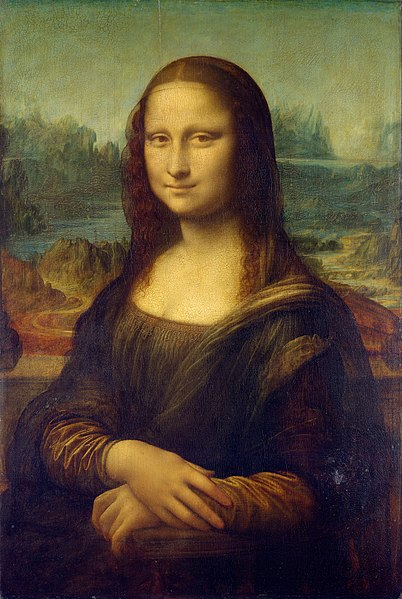
\includegraphics[width=0.45\textwidth]{monalisa}
	\caption[Mona Lisa, again]{It's Mona Lisa again. \blindtext}
	\labfig{normalmonalisa}
\end{figure}

While the format of the caption is managed by \Package{caption}, its 
position is handled by the \Package{floatrow} package. Achieving this 
result has been quite hard, but now I am pretty satisfied. In two-side 
mode, the captions are printed in the correct margin.

Tables can be inserted just as easily as figures, as exemplified by the 
following code:

\begin{lstlisting}[caption={Caption of a listing.}]
\begin{table}
\begin{tabular}{ c c c c }
	\toprule
	col1 & col2 & col3 & col 4 \\
	\midrule
	\multirow{3}{4em}{Multiple row} & cell2 & cell3 & cell4\\ &
	cell5 & cell6 & cell7 \\ &
	cell8 & cell9 & cell10 \\
	\multirow{3}{4em}{Multiple row} & cell2 & cell3 & cell4 \\ &
	cell5 & cell6 & cell7 \\ &
	cell8 & cell9 & cell10 \\
	\bottomrule
\end{tabular}
\end{table}
\end{lstlisting}

which results in the useless \vreftab{useless}.

\begin{table}[ht]
\caption[A useless table]{A useless table.}
\labtab{useless}
\begin{tabular}{ c c c c }
	\toprule
	col1 & col2 & col3 & col 4 \\
	\midrule
	\multirow{3}{4em}{Multiple row} & cell2 & cell3 & cell4\\ &
	cell5 & cell6 & cell7 \\ &
	cell8 & cell9 & cell10 \\
	\multirow{3}{4em}{Multiple row} & cell2 & cell3 & cell4 \\ &
	cell5 & cell6 & cell7 \\ &
	cell8 & cell9 & cell10 \\
	\bottomrule
\end{tabular}
\end{table}

I don't have much else to say, so I will just insert some blind text. 
\blindtext

\section{Margin Figures and Tables}

Marginfigures can be inserted with the environment 
\Environment{marginfigure}. In this case, the whole picture is confined 
to the margin and the caption is below it. \reffig{marginmonalisa} is 
obtained with something like this:

\begin{lstlisting}[caption={Another caption.}]
\begin{marginfigure}
	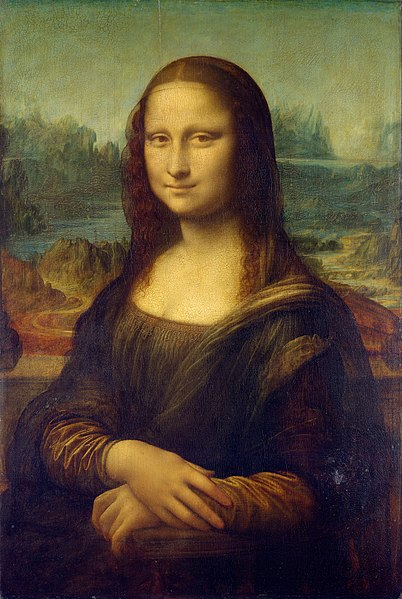
\includegraphics{monalisa}
	\caption[The Mona Lisa]{The Mona Lisa.}
	\labfig{marginmonalisa}
\end{marginfigure}
\end{lstlisting}

There is also the \Environment{margintable} environment, of which 
\reftab{anotheruseless} is an example. Notice how you can place the 
caption above the table by just placing the \Command{caption} command 
before beginning the \Environment{tabular} environment. Usually, figure 
captions are below, while table captions are above. This rule is also 
respected for normal figures and tables: the captions are always on the 
side, but for figure they are aligned to the bottom, while for tables to 
the top.

\begin{margintable}
\caption[Another useless table]{Another useless table.}
\labtab{anotheruseless}
\raggedright
\begin{tabular}{ c c c c }
	\hline
	col1 & col2 & col3 \\
	\hline
	\multirow{3}{4em}{Multiple row} & cell2 & cell3 \\ & cell5 & cell6 
	\\ & cell8 & cell9 \\ \hline
\end{tabular}
\end{margintable}

Marginfigures and tables can be positioned with an optional offset 
command, like so:

\begin{lstlisting}
\begin{marginfigure}[offset]
	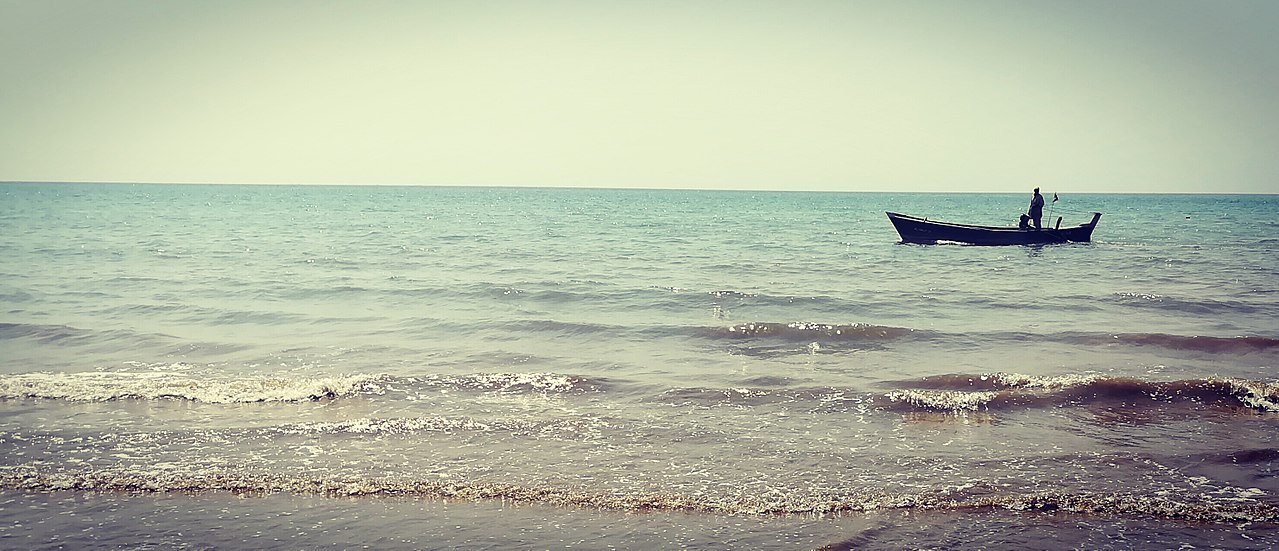
\includegraphics{seaside}
\end{marginfigure}
\end{lstlisting}

Offset ca be either a measure or a multiple of \Command{baselineskip}, 
much like with \Command{sidenote}, \Command{marginnote} and 
\Command{margintoc}.\todo{Improve this part.} If you are wondering how I 
inserted this orange bubble, have a look at the \Package{todo} package.

\section{Wide Figures and Tables}

With the environments \Environment{figure*} and \Environment{table*} you 
can insert figures which span the whole page width. For example, here 
are a wide figure and a wide table.

\begin{figure*}[h!]
	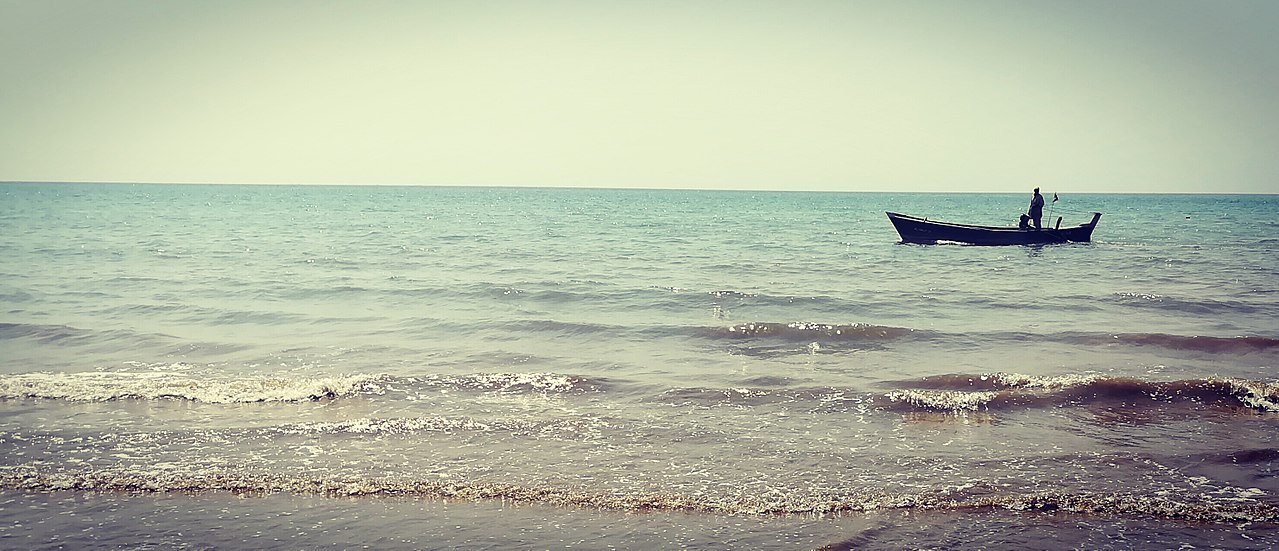
\includegraphics{seaside}
	\caption[A wide seaside]{A wide seaside, and a wide caption.
		Credits: By Bushra Feroz, CC BY-SA 4.0, \url{https://commons.wikimedia.org/w/index.php?curid=68724647}}
\end{figure*}

\begin{table*}[h!]
    \caption[Wide table example]{A wide table with invented data about three people living in the UK. Note that wide figures and tables are centered and their caption also extends into the margin.}
    \begin{tabular}{p{2.0cm} p{2.0cm} p{2.0cm} p{2.0cm} p{2.0cm} p{2.0cm} p{1.5cm}}
        \toprule
        Name    & Surname   & Job       & Salary           & Age   & Height    & Country \\
        \midrule
        Alice   & Red       & Writer    & 4.000 \pounds    & 34    & 167 cm     & England \\
        Bob     & White     & Bartender & 2.000 \pounds    & 24    & 180 cm     & Scotland \\
        Drake   & Green     & Scientist & 4.000 \pounds    & 26    & 175 cm     & Wales \\
        \bottomrule
    \end{tabular}
\end{table*}

It is the user's responsibility to adjust the width of the table, if 
necessary, until it is aesthetically pleasing. The previous table was 
obtained with the following code:

\begin{lstlisting}[caption=How to typeset a wide table]
\begin{table*}[h!]
    \caption[Wide table example]{A wide table with invented data about three people living in the UK. Note that wide figures and tables are centered and their caption also extends into the margin.}
    \begin{tabular}{p{2.0cm} p{2.0cm} p{2.0cm} p{2.0cm} p{2.0cm} p{2.0cm} p{1.5cm}}
        \toprule
        Name    & Surname   & Job       & Salary           & Age   & Height    & Country \\
        \midrule
        Alice   & Red       & Writer    & 4.000 \pounds    & 34    & 167 cm     & England \\
        Bob     & White     & Bartender & 2.000 \pounds    & 24    & 180 cm     & Scotland \\
        Drake   & Green     & Scientist & 4.000 \pounds    & 26    & 175 cm     & Wales \\
        \bottomrule
    \end{tabular}
\end{table*}
\end{lstlisting}

The \Package{floatrow} package provides the \enquote{H} specifier to 
instruct \LaTeX to position the figure (or table) in precisely the same 
position it occupies in the source code. However, this specifier does 
not work with wide figures or tables: you should use \enquote{h!} 
instead, like so: \lstinline|\begin{figure*}[h!]|.

You may have noticed the full width image at the very beginning of this
chapter: that, however, is set up in an entirely different way, which
you'll read about in \vrefch{layout}.

\Class{kaobook} also supports paginated tables (have a look at the 
\Package{longtable} package). The 
\Environment{longtable}\sidenote{Interestingly, \Environment{longtable}s 
may require up to four rounds of compilation before they are typeset 
correctly.} environment behaves a bit differently from 
\Environment{table}, in that \Environment{longtable} encompasses both 
\Environment{table} and \Environment{tabular}, so that you can write, 
\eg,

\begin{lstlisting}[caption=Example of a longtable]
\begin{longtable}{|l c c|}
    \hline
    One & Two & Three \\
    Left & Center & Center \\
    \hline
    \caption[Longtable caption]{Caption of the longtable.}
\end{longtable}
\end{lstlisting}

to obtain the following table:
\begin{longtable}{|l c c|}
    \hline
    One & Two & Three \\
    Left & Center & Center \\
    \hline
    \caption[Longtable caption]{Caption of the longtable.}
\end{longtable}

The caption of a \Environment{longtable} is always positioned below the 
table, and it has the same width as the text (it doesn't extend into the 
margin). However, sometimes you may need a \Environment{longtable} that 
is so wide that it trespass into the margins; in those cases, you may 
want to also increase the width of the caption. To do so, you'll have to 
write two additional commands, one before and one after the 
\Environment{longtable}:

\begin{lstlisting}[caption=Increasing the width of the caption of a \Environment{longtable}.]
\floatsetup[longtable]{margins=centering,LTcapwidth=table} % Add this line before the longtable to increase the caption width
\begin{longtable}{lp{8cm}p{5cm}p{2cm}}
...
\end{longtable}
\floatsetup[longtable]{margins=raggedright,LTcapwidth=\textwidth} % Add this line after the longtable to revert the previous change
\end{lstlisting}

Having seen figures and tables, it is now time to tackle 
hyperreferences.

% \setchapterstyle{kao}
%\setchapterpreamble[u]{\margintoc}
\chapter{References}
\labch{references}

\section{Citations}

\index{citations}
To cite someone \sidecite{Visscher2008,James2013} is very simple: just 
use the \Command{sidecite}\index{\Command{sidecite}} command. It does 
not have an offset argument yet, but it probably will in the future. 
This command supports multiple entries, as you can see, and by default 
it prints the reference on the margin as well as adding it to the 
bibliography at the end of the document. Note that the citations have 
nothing to do with the text,\sidecite{James2013} but they are completely 
random as they only serve the purpose to illustrate the feature.

For this setup I wrote a separate package, \Package{kaobiblio}, which 
you can find in the \Package{styles} directory and include in your main 
tex file. This package accepts all the options that you can pass to 
\Package{biblatex}, and actually it passes them to \Package{biblatex} 
under the hood. Moreover, it also defines some commands, like 
\Command{sidecite}, and environments that can be used within a 
\Class{kao} book.\sidenote[][-.9cm]{For this reason you should always 
use \Package{kaobiblio} instead of \Package{biblatex}, but the syntax 
and the options are exactly the same.}

If you want to use \Package{bibtex} instead of \Package{biblatex},
pass the option \Option{backend=bibtex} to \Package{kaobiblio}.
\Package{kaobiblio} also supports two options that are not shared with
\Package{biblatex}: \Option{addspace} and \Option{linkeverything},
both of which are boolean options, meaning that they can take
either \enquote{true} or \enquote{false} as a value. If you
pass \Option{addspace=true} when loading \Package{kaobiblio},
a space will be automatically added before the citation marks.
If you pass \Option{linkeverything=true}, the author's name in
the authoryear-* and authortitle-* styles will be a hyperlink
like the year.\sidenote{The fact that the author name is not
a hyperlink bothers more than one biblatex user. There are
\href{https://github.com/plk/biblatex/issues/428}{strong arguments}
\emph{against} hyperlinking the author name, but in my personal opinion, 
linking the author's name does not result in any problems in most 
practical cases.}

As you have seen, the \Command{sidecite} command will print a citation 
in the margin. However, this command would be useless without a way to 
customise the format of the citation, so the \Class{kaobook} provides 
also the \Command{formatmargincitation} command. By \enquote{renewing} 
that command, you can choose which items will be printed in the margins. 
The best way to understand how it works is to see the actual definition 
of this command.

\begin{lstlisting}[style=kaolstplain,linewidth=1.5\textwidth]
\newcommand{\formatmargincitation}[1]{%
	\parencite{#1}: \citeauthor*{#1} (\citeyear{#1}), \citetitle{#1}%
}
\end{lstlisting}

Thus, the \Command{formatmargincitation} accepts one parameter, which is 
the citation key, and prints the parencite followed by a colon, then the 
author, then the year (in brackets), and finally the 
title.\sidecite{Battle2014} Now, suppose that you wish the margin 
citation to display the year and the author, followed by the title, and 
finally a fixed arbitrary string; you would add to your document:

\begin{lstlisting}[style=kaolstplain,linewidth=1.5\textwidth]
\renewcommand{\formatmargincitation}[1]{%
	\citeyear{#1}, \citeauthor*{#1}: \citetitle{#1}; very interesting!%
}
\end{lstlisting}

\renewcommand{\formatmargincitation}[1]{%
	\citeyear{#1}, \citeauthor*{#1}: \citetitle{#1}; very interesting!%
}

The above code results in citations that look like the 
following.\sidecite{Zou2005} Of course, changing the format is most 
useful when you also change the default bibliography style. For 
instance, if you want to use the \enquote{philosophy-modern} style for 
your bibliography, you might have something like this in the preamble:

\begin{lstlisting}[style=kaolstplain,linewidth=1.5\textwidth]
\usepackage[style=philosophy-modern]{styles/kaobiblio}
\renewcommand{\formatmargincitation}[1]{%
	\sdcite{#1}%
}
\addbibresource{main.bib}
\end{lstlisting}

\renewcommand{\formatmargincitation}[1]{%
	\parencite{#1}: \citeauthor*{#1} (\citeyear{#1}), \citetitle{#1}%
}

The commands like \Command{citeyear}, \Command{parencite}
and \Command{sdcite} are just examples. A full
reference of the available commands can be found in this
\href{http://tug.ctan.org/info/biblatex-cheatsheet/biblatex-cheatsheet.pdf}{cheatsheet},
under the \enquote{Citations} section.

Finally, to compile a document containing citations, you need to use an 
external tool, which for this class is biber. You need to run the 
following (assuming that your tex file is called main.tex):

\begin{lstlisting}[style=kaolstplain]
$ pdflatex main
$ biber main
$ pdflatex main
\end{lstlisting}

\section{Glossaries and Indices}

\index{glossary}
The \Class{kaobook} class loads the packages \Package{glossaries} and 
\Package{imakeidx}, with which you can add glossaries and indices to 
your book. For instance, I previously defined some glossary entries and 
now I am going to use them, like this: \gls{computer}. 
\Package{glossaries} also allows you to use acronyms, like the 
following: this is the full version, \acrfull{fpsLabel}, and this is the 
short one \acrshort{fpsLabel}. These entries will appear in the glossary 
in the backmatter.

Unless you use \href{https://www.overleaf.com}{Overleaf} or some other 
fancy IDE for \LaTeX, you need to run an external command from your 
terminal in order to compile a document with a glossary. In particular, 
the commands required are:\sidenote{These are the commands you would run 
in a UNIX system, but see also \nrefsec{compiling}; I have no idea about 
how it works in Windows.}

\begin{lstlisting}[style=kaolstplain]
$ pdflatex main
$ makeglossaries main
$ pdflatex main
\end{lstlisting}

Note that you need not run \texttt{makeglossaries} every time you 
compile your document, but only when you change the glossary entries.

\index{index}
To create an index, you need to insert the command 
\lstinline|\index{subject}| whenever you are talking about 
\enquote{subject} in the text. For instance, at the start of this 
paragraph I would write \lstinline|index{index}|, and an entry would be 
added to the Index in the backmatter. Check it out!

\marginnote[2mm]{In theory, you would need to run an external command 
for the index as well, but luckily the package we suggested, 
	\Package{imakeidx}, can compile the index automatically.}

\index{nomenclature}
A nomenclature is just a special kind of index; you can find one at the end of
this book. To insert a nomenclature, we use the package \Package{nomencl} and
add the terms with the command \Command{nomenclature}. We put then a
\Command{printnomenclature} where we want it to appear.

Also with this package we need to run an external command to compile the 
document, otherwise the nomenclature will not appear:

\begin{lstlisting}[style=kaolstplain]
$ pdflatex main
$ makeindex main.nlo -s nomencl.ist -o main.nls
$ pdflatex main
\end{lstlisting}

These packages are all loaded in 
\href{style/packages.sty}{packages.sty}, one of the files that come with 
this class. However, the configuration of the elements is best done in 
the main.tex file, since each book will have different entries and 
styles.

Note that the \Package{nomencl} package caused problems when the 
document was compiled, so, to make a long story short, I had to prevent 
\Package{scrhack} to load the hack-file for \Package{nomencl}. When 
compiling the document on Overleaf, however, this problem seem to 
vanish.

\marginnote[-19mm]{This brief section was by no means a complete 
reference on the subject, therefore you should consult the documentation 
of the above package to gain a full understanding of how they work.}

\section{Hyperreferences}
\labsec{hyprefs}

\index{hyperreferences}
Together with this class we provide a handy package to help you 
referencing the same elements always in the same way, for consistency 
across the book. First, you can label each element with a specific 
command. For instance, should you want to label a chapter, you would put 
\lstinline|\labch{chapter-title}| right after the \Command{chapter} 
directive. This is just a convenience, because \Command{labch} is
actually just an alias to \lstinline|\label{ch:chapter-title}|, so it 
spares you the writing of \enquote{ch:}. We defined similar commands for 
many typically labeled elements, including:

\begin{multicols}{2}
\setlength{\columnseprule}{0pt}
\begin{itemize}
	\item Page: \Command{labpage}
	\item Part: \Command{labpart}
	\item Chapter: \Command{labch}
	\item Section: \Command{labsec}
	\item Figure: \Command{labfig}
	\item Table: \Command{labtab}
	\item Definition: \Command{labdef}
	\item Assumption: \Command{labassum}
	\item Theorem: \Command{labthm}
	\item Proposition: \Command{labprop}
	\item Lemma: \Command{lablemma}
	\item Remark: \Command{labremark}
	\item Example: \Command{labexample}
	\item Exercise: \Command{labexercise}
\end{itemize}
\end{multicols}

Of course, we have similar commands for referencing those elements. 
However, since the style of the reference should depend on the context, 
we provide different commands to reference the same thing. For instance, 
in some occasions you may want to reference the chapter by name, but 
other times you want to reference it only by number. In general, there 
are four reference style, which we call plain, vario, name, and full.

The plain style references only by number. It is accessed, for chapters, 
with \lstinline|\refch{chapter-title}| (for other elements, the syntax 
is analogous). Such a reference results in: \refch{references}.

The vario and name styles rest upon the \Package{varioref} package. 
Their syntax is \lstinline|\vrefch{chapter-title}| and 
\lstinline|\nrefch{chapter-title}|, and they result in: 
\vrefch{references}, for the vario style, and: \nrefch{references}, for 
the name style. As you can see, the page is referenced in 
\Package{varioref} style.

The full style references everything. You can use it with 
\lstinline|\frefch{chapter-title}| and it looks like this: 
\frefch{references}.

Of course, all the other elements have similar commands (\eg for parts 
you would use \lstinline|\vrefpart{part-title}| or something like that). 
However, not all elements implement all the four styles. The commands 
provided should be enough, but if you want to see what is available or 
to add the missing ones, have a look at the 
\href{styles/kaorefs.sty}{attached package}.

In order to have access to all these features, the \Package{kaorefs} 
should be loaded in the preamble of your document. It should be loaded 
last, or at least after \Package{babel} (or \Package{polyglossia}) and 
\Package{plaintheorems} (or \Package{mdftheorems}). Options can be 
passed to it like to any other package; in particular, it is possible to 
specify the language of the captions. For instance, if you specify 
\enquote{italian} as an option, instead of \enquote{Chapter} it will be 
printed \enquote{Capitolo}, the Italian analog. If you know other 
languages, you are welcome to contribute the translations of these 
captions! Feel free to contact the author of the class for further 
details. 

The \Package{kaorefs} package also include \Package{cleveref}, so it is 
possible to use \Command{cref} in addition to all the previously 
described referencing commands.

\section{A Final Note on Compilation}
\labsec{compiling}

Probably the easiest way to compile a latex document is with the 
\Package{latexmk} script, as it can take care of everything, if properly 
configured, from the bibliography to the glossary. The command to issue, 
in general, is:

\begin{lstlisting}
latexmk [latexmk_options] [filename ...]
\end{lstlisting}

\Package{latexmk} can be extensively configured (see
\url{https://mg.readthedocs.io/latexmk.html}). For convenience, I print 
here an example configuration that would cover all the steps described 
above.

\begin{lstlisting}
# By default compile only the file called 'main.tex'
@default_files = ('main.tex');

# Compile the glossary and acronyms list (package 'glossaries')
add_cus_dep( 'acn', 'acr', 0, 'makeglossaries' );
add_cus_dep( 'glo', 'gls', 0, 'makeglossaries' );
$clean_ext .= " acr acn alg glo gls glg";
sub makeglossaries {
   my ($base_name, $path) = fileparse( $_[0] );
   pushd $path;
   my $return = system "makeglossaries", $base_name;
   popd;
   return $return;
}

# Compile the nomenclature (package 'nomencl')
add_cus_dep( 'nlo', 'nls', 0, 'makenlo2nls' );
sub makenlo2nls {
    system( "makeindex -s nomencl.ist -o \"$_[0].nls\" \"$_[0].nlo\"" );
}
\end{lstlisting}

However, if you'd rather not use an external package and want to do 
everything manually, here are some tips.\sidenote{As the author only 
uses Linux and compiles everything from the command line, he doesn't 
know how the compilation works in Windows or Mac. The tips, therefore, 
refer to the usage with Linux from the command line.}

\minisec{Compiling the examples in the kaobook repository}
To compile the examples, and in particular the documentation, that are 
in the \Path{examples} directory of the 
\href{https://github.com/fmarotta/kaobook}{kaobook repository} on 
GitHub, do as follows. \lstinline[language=bash]|cd| into the root 
directory of the repository, and run
\lstinline|pdflatex -output-directory examples/documentation main.tex|. 
With this trick, you can compile the documentation using the class files 
pertaining to the repository (and not, say, those in your texmf tree). 
The \enquote{-output-directory} option works with the other 
\LaTeX-related commands such as biber and makeglossaries.

A note of warning: sometimes \LaTeX\ needs more than one run to get the
correct position of each element; this is true in particular for the
positioning of floating elements like figures, tables, and margin notes.
Occasionally, \LaTeX\ can need up to four re-runs, so If the alignment
of margin elements looks odd, or if they bleed into ther main text, try
runnign pdflatex one more time.


% \pagelayout{wide} % No margins
% \addpart{Design and Additional Features}
% \pagelayout{margin} % Restore margins

% \setchapterimage[6cm]{seaside}
\setchapterpreamble[u]{\margintoc}
\chapter{Page Design}
\labch{layout}

\section{Headings}

So far, in this document I used two different styles for the chapter 
headings: one has the chapter name, a rule and, in the margin, the 
chapter number; the other has an image at the top of the page, and the 
chapter title is printed in a box (like for this chapter). There is one 
additional style, which I used only in the \nrefch{appendix}; there, the chapter title is enclosed in two 
horizontal rules, and the chapter number (or letter, in the case of the 
appendix) is above it.\sidenote{To be honest, I do not think that mixing 
heading styles like this is a wise choice, but in this document I did it 
only to show you how they look.}

Every book is unique, so it makes sense to have different styles from 
which to choose. Actually, it would be awesome if whenever a 
\Class{kao}-user designs a new heading style, he or she added it to the 
three styles already present, so that it will be available for new users 
and new books.

The choice of the style is made simple by the \Command{setchapterstyle} 
command. It accepts one option, the name of the style, which can be: 
\enquote{plain}, \enquote{kao}, \enquote{bar}, or 
\enquote{lines}.\sidenote{Plain is the default \LaTeX\xspace title 
style; the other ones are self explanatory.} If instead you want the 
image style, you have to use the command \Command{setchapterimage}, 
which accepts the path to the image as argument; you can also provide an 
optional parameter in square brackets to specify the height of the 
image. \Command{setchapterimage} automatically sets the chapter style to 
\enquote{bar} for that chapter (and also for subsequent chapters).

Let us make some examples. In this book, I begin a normal chapter with 
the lines:
\begin{lstlisting}
\setchapterstyle{kao}
\setchapterpreamble[u]{\margintoc}
\chapter{Title of the Chapter}
\labch{title}
\end{lstlisting}

In Line 1 I choose the style for the title to be \enquote{kao}. Then, I 
specify that I want the margin toc. The rest is ordinary administration 
in \LaTeX, except that I use my own \Command{labch} to label the 
chapter. Actually, the \Command{setchapterpreamble} is a standard 
\KOMAScript\xspace one, so I invite you to read about it in the KOMA
documentation. Once the chapter style is set, it holds until you change 
it.\sidenote{The \Command{margintoc} has to be specified at every 
chapter. Perhaps in the future this may change; it all depends on how 
this feature will be welcomed by the users, so keep in touch with me if 
you have preferences!} Whenever I want to start a chapter with an image, 
I simply write:

\begin{lstlisting}
\setchapterimage[7cm]{path/to/image.png} % Optionally specify the height
\setchapterpreamble[u]{\margintoc}
\chapter{Catchy Title} % No need to set a chapter style
\labch{catchy}
\end{lstlisting}

If you prefer, you can also specify the style at the beginning of the 
main document, and that style will hold until you change it again.

\section{Headers \& Footers}

Headers and footers in \KOMAScript\xspace are handled by the 
\Package{scrlayer-scrpage} package. There are two basic style: 
\enquote{scrheadings} and \enquote{plain.scrheadings}. The former is 
used for normal pages, whereas the latter is used in title pages (those 
where a new chapter starts, for instance) and, at least in this book, in 
the front matter. At any rate, the style can be changed with the 
\Command{pagestyle} command, \eg 
\lstinline|\pagestyle{plain.scrheadings}|.

In both styles, the footer is completely empty. In plain.scrheadings,
also the header is absent (otherwise it wouldn't be so plain\ldots), but 
in the normal style the design is reminiscent of the \enquote{kao} style
for chapter titles.

\begin{kaobox}[frametitle=To Do]
The \Option{twoside} class option is still unstable and may lead to 
unexpected behaviours. As always, any help will be greatly appreciated.
\end{kaobox}

\section{Table of Contents}

Another important part of a book is the table of contents. By default, 
in \Class{kaobook} there is an entry for everything: list of figures, 
list of tables, bibliographies, and even the table of contents itself. 
Not everybody might like this, so we will provide a description of the 
changes you need to do in order to enable or disable each of these 
entries. In the following \reftab{tocentries}, each item corresponds to 
a possible entry in the \acrshort{tocLabel}, and its description is the 
command you need to provide to have such entry. These commands are 
specified in the attached \href{style/style.sty}{style 
package},\sidenote{In the same file, you can also choose the titles of 
these entries.} so if you don't want the entries, just comment the 
corresponding lines.

Of course, some packages, like those for glossaries and indices, will 
try to add their own entries.\marginnote{In a later section, we will see 
how you can define your own floating environment, and endow it with an 
entry in the \acrshort{tocLabel}.} In such cases, you have to follow the 
instructions specific to that package. Here, since we have talked about 
glossaries and notations in \refch{references}, we will briefly see how
to configure them.

\begin{table}
\footnotesize
\caption[TOC entry commands]{Commands to add a particular entry to the table of contents.}
\labtab{tocentries}
\begin{tabular}{ l l }
	\toprule
	Entry & Command to Activate \\
	\midrule
	Table of Contents & \lstinline|\setuptoc{toc}{totoc}| \\
	List of Figs and Tabs & \lstinline|\PassOptionsToClass{toc=listof}{\@baseclass}| \\
	Bibliography & \lstinline|\PassOptionsToClass{toc=bibliography}{\@baseclass}| \\
	\bottomrule
\end{tabular}
\end{table}

For the \Package{glossaries} package, use the \enquote{toc} option when 
you load it: \lstinline|\usepackage[toc]{glossaries}|. For 
\Package{nomencl}, pass the \enquote{intoc} option at the moment of 
loading the package. Both \Package{glossaries} and \Package{nomencl} are 
loaded in the attached \href{style/packages.sty}{\enquote{packages} 
package}.

Additional configuration of the table of contents can be performed 
through the packages \Package{etoc}, which is loaded because it is 
needed for the margintocs, or the more traditional \Package{tocbase}. 
Read the respective documentations if you want to be able to change the 
default \acrshort{tocLabel} style.\sidenote[][*-1]{(And please, send me 
a copy of what you have done, I'm so curious!)}

\section{Paper Size}

Recent versions of Kaobook support paper sizes different from the
default A4. It is possible to pass the name of the paper as an option
to the class, as we are accustomed for any other \LaTeX\ class. For
example, the class option \Option{b5paper} would set the paper size
to the B5 format.

We also support the paper sizes specified in
\href{https://www.bod.de/hilfe/hilfe-und-service.html?cmd=SINGLE\&entryID=2494\_GER\_WSS\&eo=2\&title=welche-buchformate-gibt-es}{this
web page} and some additional sizes requested by the users, with the 
option names specified in \reftab{papersizes}.

\begin{margintable}[*-6]
	\caption[Non-standard paper sizes]{Some non-standard paper sizes supported by kaobook.}
	\labtab{papersizes}
	\begin{tabular}{ll}
		\toprule
		Dimension & Option name \\
		\midrule
		12.0cm x 19.0cm & smallpocketpaper \\
		13.5cm x 21.5cm & pocketpaper \\
		14.8cm x 21.0cm & a5paper \\
		15.5cm x 22.0cm & juvenilepaper \\
		17.0cm x 17.0cm & smallphotopaper \\
		21.0cm x 15.0cm & appendixpaper \\
		17.0cm x 22.0cm & cookpaper \\
		19.0cm x 27.0cm & illustratedpaper \\
		17.0cm x 17.0cm & photopaper \\
		16.0cm x 24.0cm & f24paper \\
		%21.0cm x 29.7cm & a4paper \\
		\bottomrule
	\end{tabular}
\end{margintable}

For instance, to use the \enquote{smallpocketpaper} add the correct 
description at the beginning of the documentclass instruction:
\begin{lstlisting}
\documentclass[
		smallpocketpaper,
		fontsize=10pt,
		twoside=false,
		%open=any,
		secnumdepth=1,
]{kaobook}
\end{lstlisting}

\section{Page Layout}

Besides the page style, you can also change the width of the content of 
a page. This is particularly useful for pages dedicated to part titles, 
where having the 1.5-column layout might be a little awkward, or for 
pages where you only put figures, where it is important to exploit all 
the available space.

In practice, there are two layouts: \enquote{wide} and \enquote{margin}. 
The former suppresses the margins and allocates the full page for 
contents, while the latter is the layout used in most of the pages of 
this book, including this one. The wide layout is also used 
automatically in the front and back matters.

\marginnote{Sometimes it is desirable to increase the width for just one 
or a few paragraphs; the \Environment{widepar} environment does that: 
wrap your paragraphs in this environment, and they will occupy the full 
width of the page.}

To change page layout, use the \Command{pagelayout} command. For 
example, when I start a new part, I write:

\begin{lstlisting}
\pagelayout{wide}
\addpart{Title of the New Part}
\pagelayout{margin}
\end{lstlisting}

Beyond these two basic layouts, it is also possible to finely tune the 
page layout by redefining the \Command{marginlayout} command. This 
command is called internally by the higher-level \Command{pagelayout}, 
and it is responsible for setting the width of the margins and of the 
text. The default definition is:

\begin{lstlisting}
\newcommand{\marginlayout}{%
	\newgeometry{
		top=27.4mm,				% height of the top margin
		bottom=27.4mm,			% height of the bottom margin
		inner=24.8mm,			% width of the inner margin
		textwidth=107mm,		% width of the text
		marginparsep=8.2mm,		% width between text and margin
		marginparwidth=49.4mm,	% width of the margin
	}%
}
\end{lstlisting}

so if you want to, say, decrease the width of the margin while 
increasing the width of the text, you could write in the preamble of 
your document something like:

\begin{lstlisting}
\renewcommand{\marginlayout}{%
	\newgeometry{
		top=27.4mm,				% height of the top margin
		bottom=27.4mm,			% height of the bottom margin
		inner=24.8mm,			% width of the inner margin
		textwidth=117mm,		% width of the text
		marginparsep=8.2mm,		% width between text and margin
		marginparwidth=39.4mm,	% width of the margin
	}%
}
\end{lstlisting}

where the text width has been increased by 10mm and the margin width has 
been decreased by 10mm.

\section{Numbers \& Counters}

In this short section we shall see how dispositions, sidenotes and 
figures are numbered in the \Class{kaobook} class.

By default, dispositions are numbered up to the section in \Class{kaobook}
and up to the subsection in \Class{kaohandt}. This can be changed by
passing the option \Option{secnumdepth} to\Class{kaobook} or
\Class{kaohandt} (e.g. 1 corresponds to section and 2 corresponds to
subsections).

The sidenotes counter is the same across all the document, but if you 
want it to reset at each chapter, just uncomment the line

\begin{lstlisting}[style=kaolstplain]
\counterwithin*{sidenote}{chapter}
\end{lstlisting}

in the \Package{styles/style.sty} package provided by this class.

Figure and Table numbering is also per-chapter; to change that, use 
something like:

\begin{lstlisting}[style=kaolstplain]
\renewcommand{\thefigure}{\arabic{section}.\arabic{figure}}
\end{lstlisting}

\section{White Space}

One of the things that I find most hard in \LaTeX\xspace is to finely 
tune the white space around objects. There are not fixed rules, each 
object needs its own adjustment. Here we shall see how some spaces are 
defined at the moment in this class.\marginnote{Attention! This section 
may be incomplete.}

\textbf{Space around sidenotes and citations marks}

There should be no space before or after sidenotes and citation marks, 
like so:

sidenote\sidenote{This paragraph can be used to diagnose any problems:
if you see whitespace around sidenotes or citation marks, probably
a \% sign is missing somewhere in the definitions of the class
macros.}sidenote\newline
citation\cite{James2013}citation

\textbf{Space around figures and tables}

\begin{lstlisting}[style=kaolstplain]
\renewcommand\FBaskip{.4\topskip}
\renewcommand\FBbskip{\FBaskip}
\end{lstlisting}

\textbf{Space around captions}

\begin{lstlisting}[style=kaolstplain]
\captionsetup{
	aboveskip=6pt,
	belowskip=6pt
}
\end{lstlisting}

\textbf{Space around displays (\eg equations)}

\begin{lstlisting}[style=kaolstplain]
\setlength\abovedisplayskip{6pt plus 2pt minus 4pt}
\setlength\belowdisplayskip{6pt plus 2pt minus 4pt}
\abovedisplayskip 10\p@ \@plus2\p@ \@minus5\p@
\abovedisplayshortskip \z@ \@plus3\p@
\belowdisplayskip \abovedisplayskip
\belowdisplayshortskip 6\p@ \@plus3\p@ \@minus3\p@
\end{lstlisting}

% \setchapterstyle{kao}
\setchapterpreamble[u]{\margintoc}
\chapter{Mathematics and Boxes}
\labch{mathematics}

\section{Theorems}

Despite most people complain at the sight of a book full of equations, 
mathematics is an important part of many books. Here, we shall 
illustrate some of the possibilities. We believe that theorems, 
definitions, remarks and examples should be emphasised with a shaded 
background; however, the colour should not be to heavy on the eyes, so 
we have chosen a sort of light yellow.\sidenote{The boxes are all of the 
same colour here, because we did not want our document to look like 
\href{https://en.wikipedia.org/wiki/Harlequin}{Harlequin}.}

\begin{definition}
\labdef{openset}
Let $(X, d)$ be a metric space. A subset $U \subset X$ is an open set 
if, for any $x \in U$ there exists $r > 0$ such that $B(x, r) \subset 
U$. We call the topology associated to d the set $\tau\textsubscript{d}$ 
of all the open subsets of $(X, d).$
\end{definition}

\refdef{openset} is very important. I am not joking, but I have inserted 
this phrase only to show how to reference definitions. The following 
statement is repeated over and over in different environments.

\begin{theorem}
A finite intersection of open sets of (X, d) is an open set of (X, d), 
i.e $\tau\textsubscript{d}$ is closed under finite intersections. Any 
union of open sets of (X, d) is an open set of (X, d).
\end{theorem}

\begin{proposition}
A finite intersection of open sets of (X, d) is an open set of (X, d), 
i.e $\tau\textsubscript{d}$ is closed under finite intersections. Any 
union of open sets of (X, d) is an open set of (X, d).
\end{proposition}

\marginnote{You can even insert footnotes inside the theorem 
environments; they will be displayed at the bottom of the box.}

\begin{lemma}
A finite intersection\footnote{I'm a footnote} of open sets of (X, d) is 
an open set of (X, d), i.e $\tau\textsubscript{d}$ is closed under 
finite intersections. Any union of open sets of (X, d) is an open set of 
(X, d).
\end{lemma}

You can safely ignore the content of the theorems\ldots I assume that if 
you are interested in having theorems in your book, you already know 
something about the classical way to add them. These example should just 
showcase all the things you can do within this class.

\begin{corollary}[Finite Intersection, Countable Union]
A finite intersection of open sets of (X, d) is an open set of (X, d), 
i.e $\tau\textsubscript{d}$ is closed under finite intersections. Any 
union of open sets of (X, d) is an open set of (X, d).
\end{corollary}

\begin{proof}
The proof is left to the reader as a trivial exercise. Hint: \blindtext
\end{proof}

\begin{definition}
Let $(X, d)$ be a metric space. A subset $U \subset X$ is an open set 
if, for any $x \in U$ there exists $r > 0$ such that $B(x, r) \subset 
U$. We call the topology associated to d the set $\tau\textsubscript{d}$ 
of all the open subsets of $(X, d).$
\end{definition}

\marginnote{
	Here is a random equation, just because we can:
	\begin{equation*}
  x = a_0 + \cfrac{1}{a_1
          + \cfrac{1}{a_2
          + \cfrac{1}{a_3 + \cfrac{1}{a_4} } } }
	\end{equation*}
}

\begin{example}
Let $(X, d)$ be a metric space. A subset $U \subset X$ is an open set 
if, for any $x \in U$ there exists $r > 0$ such that $B(x, r) \subset 
U$. We call the topology associated to d the set $\tau\textsubscript{d}$ 
of all the open subsets of $(X, d).$
\end{example}

\begin{remark}
Let $(X, d)$ be a metric space. A subset $U \subset X$ is an open set 
if, for any $x \in U$ there exists $r > 0$ such that $B(x, r) \subset 
U$. We call the topology associated to d the set $\tau\textsubscript{d}$ 
of all the open subsets of $(X, d).$
\end{remark}

As you may have noticed, definitions, example and remarks have 
independent counters; theorems, propositions, lemmas and corollaries 
share the same counter.

\begin{remark}
Here is how an integral looks like inline: $\int_{a}^{b} x^2 dx$, and 
here is the same integral displayed in its own paragraph:
\[\int_{a}^{b} x^2 dx\]
\end{remark}

There is also an environment for exercises.

\begin{exercise}
Prove (or disprove) the Riemann hypothesis.
\end{exercise}

We provide one package for the theorem styles: 
\href{kaotheorems.sty}{kaotheorems.sty}, to which you can pass the 
\Option{framed} option you do want coloured boxes around theorems, like 
in this document.\sidenote{The styles without \Option{framed} are not 
showed, but actually the only difference is that they don't have the 
yellow boxes.} You may want to edit this files according to your taste 
and the general style of the book. However, there is an option to 
customise the background colour of the boxes if you use the 
\Option{framed} option: when you load this package, you can pass it the 
\Option{background=mycolour} option (replace \enquote{mycolour} with the 
actual colour, for instance, \enquote{red!35!white}). This will change 
the colour of all the boxes, but it is also possible to override the 
default colour only for some elements. For instance, the 
\Option{propositionbackground=mycolour} option will change the colour 
for propositions only. There are similar options for theorem, 
definition, lemma, corollary, remark, and example.

\section[Boxes \& Environments]{Boxes \& Custom Environments
\sidenote[][*1.8]{Notice that in the table of contents and in the 
	header, the name of this section is \enquote{Boxes \& Environments}; 
	we achieved this with the optional argument of the \texttt{section} 
	command.}}

Say you want to insert a special section, an optional content or just 
something you want to emphasise. We think that nothing works better than 
a box in these cases. We used \Package{mdframed} to construct the ones 
shown below. You can create and modify such environments by editing the 
provided file \href{style/environments.sty}{environments.sty}.

\begin{kaobox}[frametitle=Title of the box]
\blindtext
\end{kaobox}

If you set up a counter, you can even create your own numbered 
environment.

\begin{kaocounter}
	\blindtext
\end{kaocounter}

\section{Experiments}

It is possible to wrap marginnotes inside boxes, too. Audacious readers 
are encouraged to try their own experiments and let me know the 
outcomes.

\marginnote[-2.2cm]{
	\begin{kaobox}[frametitle=title of margin note]
		Margin note inside a kaobox.\\
		(Actually, kaobox inside a marginnote!)
	\end{kaobox}
}

I believe that many other special things are possible with the 
\Class{kaobook} class. During its development, I struggled to keep it as 
flexible as possible, so that new features could be added without too 
great an effort. Therefore, I hope that you can find the optimal way to 
express yourselves in writing a book, report or thesis with this class, 
and I am eager to see the outcomes of any experiment that you may try.

%\begin{margintable}
	%\captionsetup{type=table,position=above}
	%\begin{kaobox}
		%\caption{caption}
		%\begin{tabular}{ |c|c|c|c| }
			%\hline
			%col1 & col2 & col3 \\
			%\hline
			%\multirow{3}{4em}{Multiple row} & cell2 & cell3 \\ & cell5 
			%%& cell6 \\ 
			%& cell8 & cell9 \\
			%\hline
		%\end{tabular}
	%\end{kaobox}
%\end{margintable}


\appendix % From here onwards, chapters are numbered with letters, as is the appendix convention

\pagelayout{wide} % No margins
\addpart{Appendix}
\pagelayout{margin} % Restore margins
% \setchapterpreamble[u]{\margintoc}
\chapter{Trustworthiness Through Experiments: Copyright Traps}



\begin{kaobox}[frametitle=Paper Abstract]

Questions of fair use of copyright-protected content to train Large Language Models (LLMs) are being actively debated. Document-level inference has been proposed as a new task: inferring from black-box access to the trained model whether a piece of content has been seen during training. SOTA methods however rely on naturally occurring memorization of (part of) the content. While very effective against models that memorize significantly, we hypothesize--and later confirm--that they will not work against models that do not naturally memorize, e.g. medium-size 1B models. We here propose to use copyright traps, the inclusion of fictitious entries in original content, to detect the use of copyrighted materials in LLMs with a focus on models where memorization does not naturally occur. We carefully design a randomized controlled experimental setup, inserting traps into original content (books) and train a 1.3B LLM from scratch. We first validate that the use of content in our target model would be undetectable using existing methods. We then show, contrary to intuition, that even medium-length trap sentences repeated a significant number of times (100) are not detectable using existing methods. However, we show that longer sequences repeated a large number of times can be reliably detected (AUC=0.75) and used as copyright traps. 
Beyond copyright applications, our findings contribute to the study of LLM memorization: the randomized controlled setup enables us to draw causal relationships between memorization and certain sequence properties such as repetition in model training data and perplexity.

\end{kaobox}

\section{Introduction}





With the growing adoption of ever-improving Large Language Models (LLMs), concerns are being raised when it comes to the use of copyright protected content for training. 
Numerous content creators have indeed filed lawsuits against technology companies, claiming copyright infringement for utilizing books\sidecite{authorsguild, silvermanmeta}, songs\sidecite{anthropic} or news articles\sidecite{nytimes} for LLM development. While it is still unclear whether copyright or \emph{fair use} applies in this context\sidecite{samuelson2023generative}, model developers continue releasing new LLMs but are increasingly reluctant to disclose details on the training dataset\sidecite{openai_gpt-4_2023, touvron_llama_2023, jiang2024mixtral} - partially due to these lawsuits. 

Methods have recently been developed to detect whether a specific piece of content has been seen by an LLM during training: document-level membership inference. Both\sidecite{meeus2023did} and\sidecite{shi2023detecting} show their methods to be fairly successful against very large LLMs (up to 66B parameters), with a ROC AUC of 0.86 for OpenLLaMA\sidecite{openlm2023openllama} and 0.88 for GPT-3\sidecite{brown_language_2020}.

\begin{figure}[t]
\centering
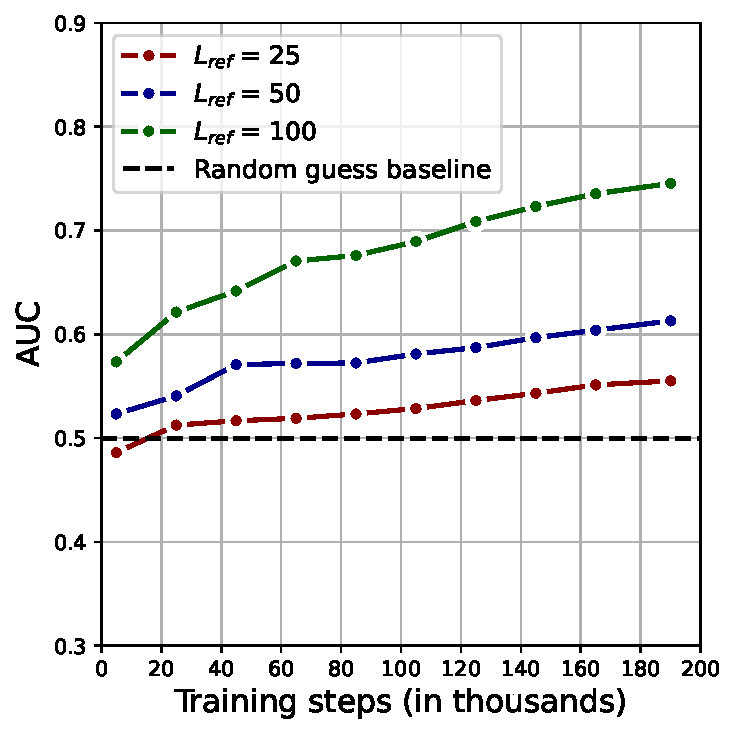
\includegraphics[width=0.6\linewidth] {images/copyright_traps_figures/MIAOverTraining.pdf} 
    \caption[Memorization throughout training]{\textbf{Memorization throughout training.} The \textit{Ratio} MIA performance (AUC) for synthetically generated trap sequences (of varying sequence length), repeated 1,000 times in a book, evaluated on intermediate checkpoints of the target LLM.}
    %The full training corresponds to 2 epochs.} 
\label{fig:across_training}
\end{figure}

Historically, original content creators have implemented so-called \emph{copyright traps} to detect copyright infringement of their work. Examples of such traps range from a fictitious street name or town on a map to the inclusion of fabricated names in a dictionary\sidecite{Alford_2005a}. In this case, the direct inclusion of these entities in other work would render a breach of copyright self-evident, while it becomes less trivial when data is aggregated, e.g. when used in machine learning models. 

We here investigate, for the first time, the use of copyright traps for document-level membership inference against LLMs. We propose the injection of purposefully designed text (\emph{trap sequences}) into a piece of content, to either further improve the performance of document-level membership inference or enable it in the first place for models less prone to memorization. 

We here focus on the latter, as recently proposed methods are already successful for larger models\sidecite{meeus2023did, shi2023detecting}, and as there is a growing trend towards smaller language models\sidecite{zhang2024tinyllama, Javaheripi_2023}. 

Specifically, we inject our traps into the training set of CroissantLLM\sidecite{faysse_croissantllm_2024}, a 1.3B parameter LLM, trained from scratch on 3 trillion tokens by the team we partnered with. Being (fairly) small and trained on significantly more data than considered in prior work on LLM memorization\sidecite{carlini2022quantifying}, we hypothesized that the model would not naturally memorize sufficiently for a document-level membership inference to succeed. Applying the two state-of-the-art methods\sidecite{meeus2023did, shi2023detecting}, we find them to perform barely better than a random guess baseline, confirming our hypothesis and rendering these methods uninformative for authors. 

We hence investigate the use of document-specific copyright traps to enable membership inference. We apply Membership Inference Attacks (MIAs) from the literature\sidecite{yeom2018privacy, carlini2021extracting, shi2023detecting} to infer whether a given trap sequence, and thus document, has been seen by a model or not.

First, we consider synthetically generated trap sequences and study the impact of number of repetitions, sequence length, and perplexity  on the post training detectability of the trap. Contrary to popular beliefs, notably from the training data extraction literature\sidecite{carlini2021extracting, nasr2023scalable}, we show that short and medium-length synthetic sequences repeated a significant number of times (100) do not help the membership inference, independently of the detection method used. We further confirm this also holds for artificially duplicated existing sentences. 

We, however, do find that the MIA AUC increases with sequence length and number of repetitions and that sequences of 100 tokens repeated 1,000 times are detectable with an AUC of 0.748. This provides the first evidence that copyright traps can be inserted in real-world LLMs to detect the use of training content otherwise undetectable.
% whose use of certain content would otherwise not be detectable. 

%In a post-hoc analysis, we demonstrate the impact of the number of times a sequence has been seen by the model on detectability. More specifically, we track the memorization during the training process, by computing the MIA AUC for our trap sequences across intermediate model checkpoints. We find that the AUC -and thus LLM memorization- increases smoothly and monotonically with the training steps, with no sign of reaching a plateau. 

We also show that sequences with high-perplexity (according to a reference model) are more likely to be detectable. The general intuition is that 'outliers' might more easily be memorized and be more vulnerable against MIAs\sidecite{feldman2020does}. We are the first to test this out for LLMs in a clean setup, and show that when memorization happens (for long sequences repeated 1,000 times), the MIA AUC improves from approximately 0.65 for low perplexity to 0.8 for high perplexity. We also show the relationship between perplexity and detectability to be a potential confounding factor in prior post-hoc studies of LLM memorization, by studying the perplexity of duplicate sequences in the large text dataset The Pile\sidecite{pile}.

Our results provide the first evidence that target-model independent copyright traps can be added to content to enable document-level membership inference, even in LLMs that would not 'naturally' memorize sufficiently to infer membership. 

While injecting traps might be not be equally trivial across document types while maintaining readability, they can be embedded across a large corpus (e.g. news articles). They can also be hidden online and not trivial to remove, especially given automated scraping and the costs associated with fine-grained deduplication for LLM training data. 


\section{Conclusion}

With the copyright concerns regarding LLM training being raised, LLM developers are reluctant to disclose details on their training data. Prior work has explored the question of document-level membership inference to detect whether a piece of content has been used to train a LLM. We first show that memorization highly depends on the training setup, as existing document-level membership inference methods fail for our 1.3B LLM. We thus propose the use of copyright traps for LLMs - purposefully designed text sequences injected into a document, intended to maximize detectability in LLM training data. 

We train a real-world, 1.3B LLM from scratch on 3 trillion tokens, containing a small set of injected trap sequences, enabling us to study their effectiveness. We find that inducing reliable memorization in a LLM is a non-trivial task. For models showing relatively low level of memorization, such as the one we train here, injecting short-to-medium sentences ($\leq $ 50 tokens) up to a 100 times does not improve document detectability. When using longer sequences, however, and up to a $1,000$ repetitions, we do see a significant effect - showing how copyright traps can enable detactability even for LLMs less prone to memorize. We further find that memorization increases with sequence perplexity, and that leveraging document-level information such as context could boost detectability. While effective, the proposed mechanism could be disruptive to the document's content and readability. Future research is thus needed, specifically in designing trap sequences maximizing detectability. We are hence committed to releasing our model and the data to further the research in the field.

% \setchapterpreamble[u]{\margintoc}
\chapter{Trustworthiness Through Confidence Estimation}
% \chapter{Revisiting Instruction Fine-tuned Model Evaluation to Guide Industrial Applications}


\begin{kaobox}[frametitle=Paper Abstract]

Neural Information Retrieval (NIR) has significantly improved upon heuristic-based Information Retrieval (IR) systems. Yet, failures remain frequent, the models used often being unable to retrieve documents relevant to the user's query. We address this challenge by proposing a lightweight abstention mechanism tailored for real-world constraints, with particular emphasis placed on the reranking phase. We introduce a protocol for evaluating abstention strategies in black-box scenarios (typically encountered when relying on API services), demonstrating their efficacy, and propose a simple yet effective data-driven mechanism. We provide open-source code for experiment replication and abstention implementation, fostering wider adoption and application in diverse contexts.

\end{kaobox}



\section{Introduction}
\label{sec:intro}

\begin{figure*}[t]
  \centering
  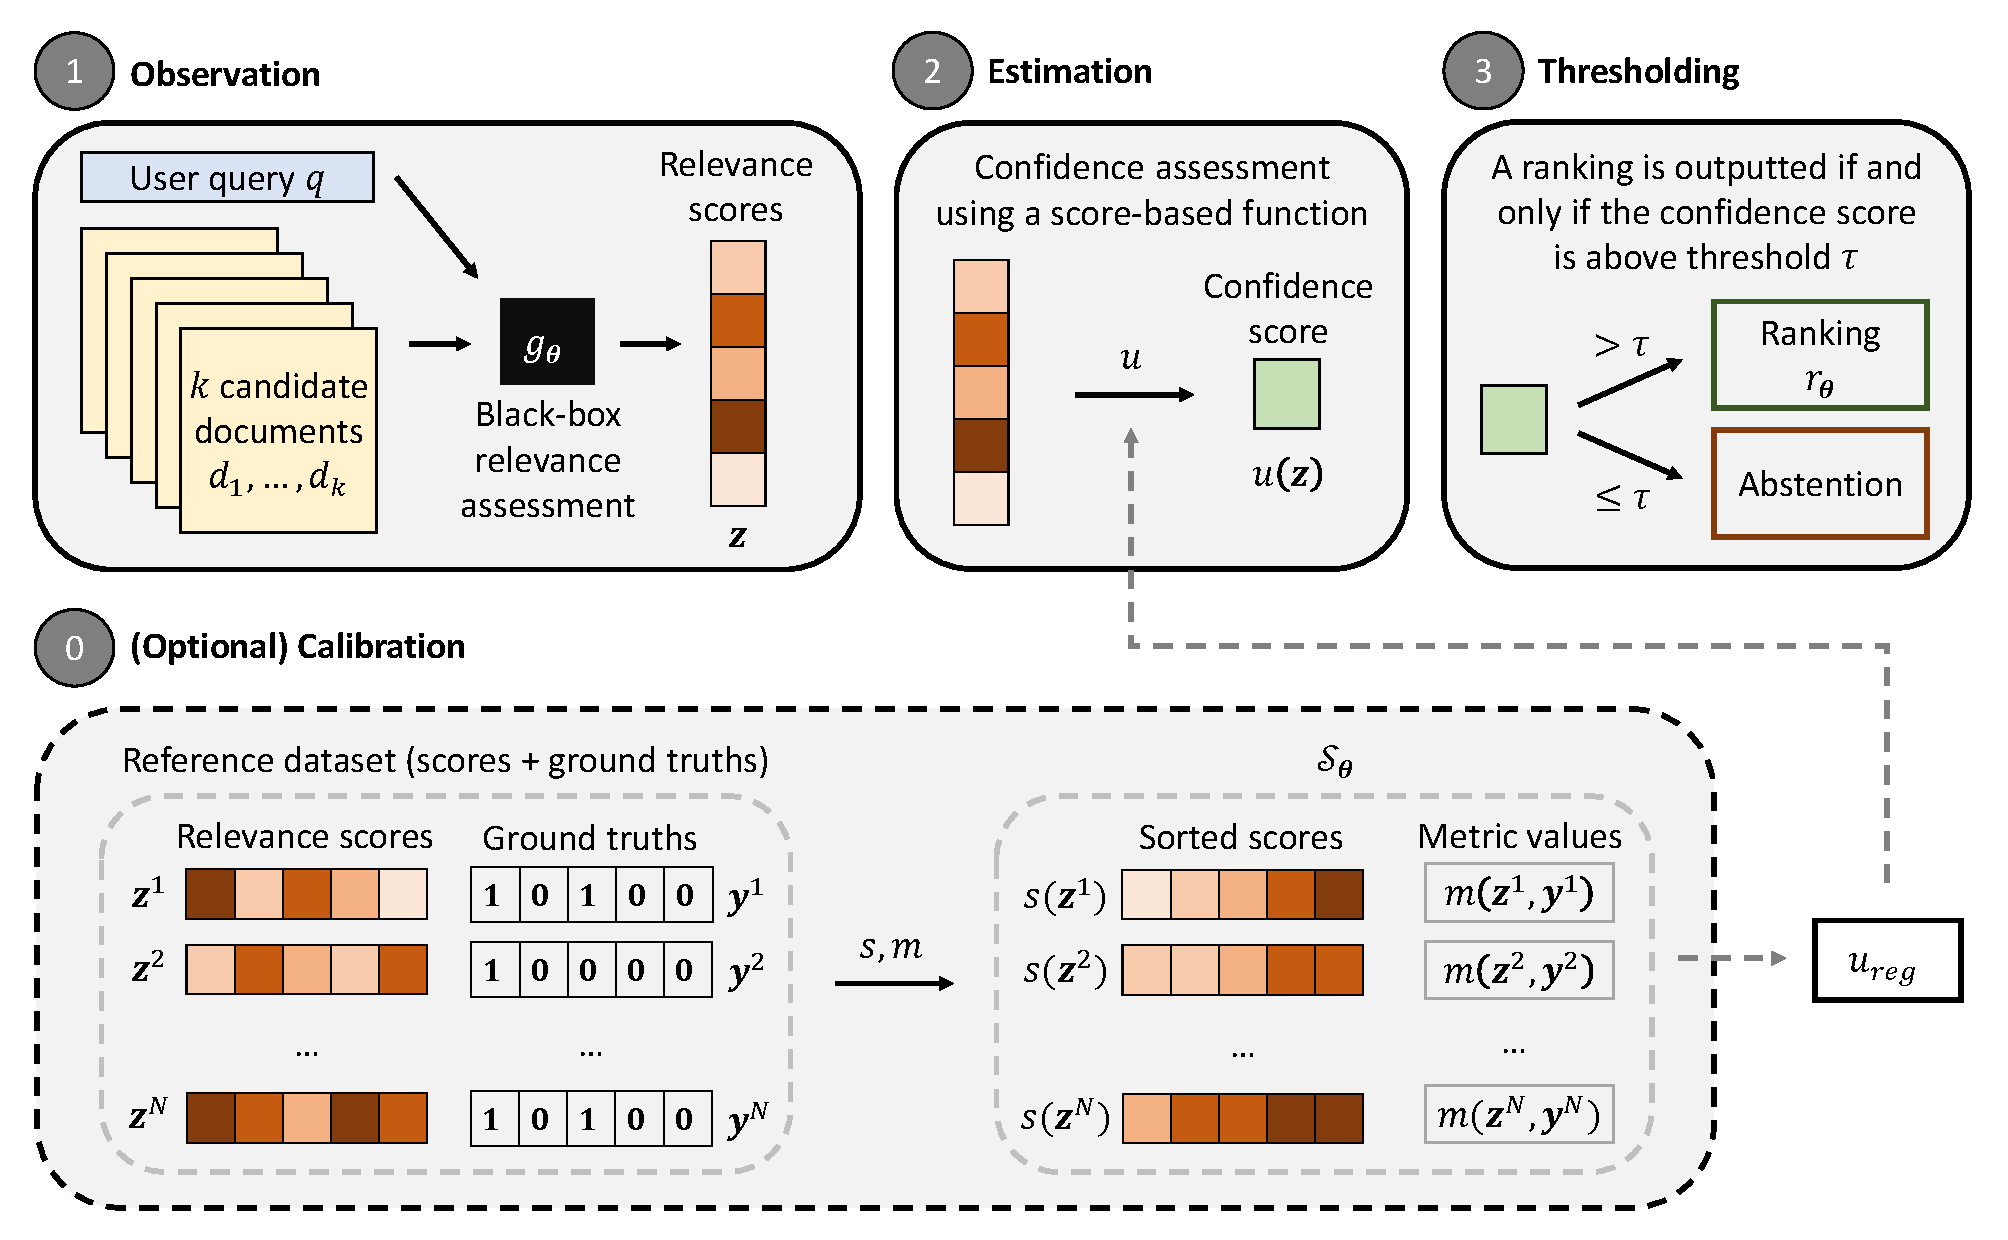
\includegraphics[width=0.85\textwidth]{images/reranking_figures/method.pdf}
  \vspace{-2mm}
  \caption[Confidence estimation procedure]{Procedure diagram for black-box confidence estimation and abstention decision in a reranking setting. In the reference-free scenario, confidence function $u$ is a simple heuristic (e.g., maximum). In the data-driven scenario, $u$ is a light non-trivial function of the relevance scores (e.g., learned linear combination).}
  \label{fig:method}
\end{figure*}

In recent years, NIR has emerged as a promising approach to addressing the challenges of IR on various tasks \sidecite{guo2016deep, mitra2017neural, zhao2022dense}. Central to the NIR paradigm are the pivotal stages of retrieval and reranking \sidecite{robertson1995okapi, ni2021large, neelakantan2022text}, which collectively play a fundamental role in shaping the performance and outcomes of IR systems \sidecite{thakur2021beir}. While the objective of the retrieval stage is to efficiently fetch candidate documents from a vast corpus based on a user's query (frequentist \sidecite{tfidf, bm25} or bi-encoder-based approaches \sidecite{karpukhin2020dense}), reranking aims at reordering these retrieved documents in a slower albeit more effective way, using more sophisticated techniques (bi-encoder- or cross-encoder-based \sidecite{nogueira2019passage, khattab2020colbert}).\sidenote{The most common approach is to have a quick retriever that scales well and a more computationally intensive reranker that reorders the top retrieved contexts.}

However, despite advancements in NIR techniques, retrieval and reranking processes frequently fail, due for instance to the quality of the models being used, to ambiguous user queries or insufficient relevant documents in the database. These can have unsuitable consequences, particularly in contexts like Retrieval-Augmented Generation (RAG) \sidecite{lewis2020retrieval}, where retrieved information is directly used in downstream tasks, thus undermining the overall system reliability \sidecite{yoran2023making, wang2023learning, baek2023knowledge}.

Recognizing the critical need to address these challenges, the implementation of abstention mechanisms emerges as a significant promise within the IR landscape. This technique offers a pragmatic approach by abstaining from delivering results when the model shows signs of uncertainty, thus ensuring users are not misled by potentially erroneous information. Although the subject of abstention in machine learning has long been of interest \sidecite{chow1957optimum, JMLR:v11:el-yaniv10a, NIPS2017_4a8423d5, pmlr-v97-geifman19a}, most research has focused on the classification setting, leaving lack of significant initiatives in IR. A few related works propose computationally intensive learning strategies \sidecite{cheng2010predicting, mao2023ranking} that are difficult to implement in the case of NIR, where models can have up to billions of parameters.

\noindent \textbf{Scope.} In this paper, we explore lightweight abstention mechanisms that adhere to realistic industrial constraints, namely  \textbf{(i)} black-box access-only to query-documents relevance scores, which is typically the case when relying on API services, \textbf{(ii)} marginal computational and latency overhead, \textbf{(iii)} configurable abstention rates depending on the application. In line with industrial applications of IR systems for RAG or search engines, our method focuses on assessing the reranking quality of the top retrieved documents.

\noindent \textbf{Contributions.} Our key contributions are:

\begin{itemize}[noitemsep, topsep=-1mm, leftmargin=8mm]
\item We devise a detailed protocol for evaluating abstention strategies in a black-box reranking setting and demonstrate their relevance. 
\item We introduce a simple yet effective reference-based abstention mechanism, outperforming reference-free heuristics at zero incurred cost. We perform ablations and analyses on this method and are confident about its potential in practical settings.
\item We release a code package and artifacts \sidenote{\url{https://github.com/artefactory/abstention-reranker}} under MIT license to enable full replication of our experiments and the implementation of plug-and-play abstention mechanisms for any use case.
\end{itemize}


\section{Problem Statement \& Related Work}

\subsection{Notations}
\label{sec:notations}

\textbf{General notations.} Let $\mathcal{V}$ denote the vocabulary and $\mathcal{V}^*$ the set of all possible textual inputs (Kleene closure of $\mathcal{V}$). Let $\mathcal{Q} \subset \mathcal{V}^*$ be the set of queries and $\mathcal{D} \subset \mathcal{V}^*$ the document database. In the reranking setting, a query $q \in \mathcal{Q}$ is associated with $k \in \mathbb{N}$ candidate documents $ \left( d_1, \cdots, d_k \right) \in \mathcal{D}^k$ coming from the preceding retrieval phase, some of them being relevant to the query and the others not. When available, we denote by $\mathbf{y} \in \left\{0,1\right\}^k$ the ground truth vector, such that $y_j = 1$ if $d_j$ is relevant to $q$ and $y_j = 0$ otherwise.\sidenote{Note that $\mathbf{y}$ is not a one-hot vector as several documents can be relevant to a single query.}

\noindent \textbf{Dataset.} When specified, we have access to a labeled reference dataset $\mathcal{S}$ composed of $N \in \mathbb{N}$ instances, each of them comprising of a query and $k$ candidate documents, $x = \left( q, d_1, \cdots, d_k \right) \in  \mathcal{Q} \times \mathcal{D}^k$, and a ground truth $\mathbf{y} \in \left\{0,1\right\}^k$. Formally, 
\begin{equation}\label{eq:dataset}
\mathcal{S} = \left \{ \left( x^i, \mathbf{y}^i \right) \right \}_{i=1}^N.
\end{equation}

\noindent \textbf{Relevance scoring.} A crucial step in the reranking task is the calculation of query-document relevance scores. We denote by $f_{\bm{\theta}} : \mathcal{Q} \times \mathcal{D} \rightarrow \mathbb{R}$ the encoder-based relevance function that maps a query-document pair to its corresponding relevance score, with $\bm{\theta} \in \Theta$ standing for the encoder parameters. We also define $g_{\bm{\theta}} : \mathcal{Q} \times \mathcal{D}^k \rightarrow \mathbb{R}^k$, the function taking a query and $k$ candidate documents as input and returning the corresponding vector of relevance scores. Formally, given $x \in  \mathcal{Q} \times \mathcal{D}^k$, 
%
\begin{equation}\label{eq:rel_scores}
g_{\bm{\theta}} \left( x \right) = \left( f_{\bm{\theta}}\left(q, d_1\right), \cdots, f_{\bm{\theta}}\left(q, d_k\right) \right).
\end{equation}

\noindent Additionally, we define the sort function $s: \mathbb{R}^k \rightarrow \mathbb{R}^k$ that takes a vector of scores as input and returns its sorted version in increasing order. For a given $\mathbf{z} \in \mathbb{R}^k$, $s(\mathbf{z})$ is such that $s_1(\mathbf{z}) \leq \cdots \leq s_k(\mathbf{z})$.\sidenote{$s_j(\mathbf{z})$ denotes the $j^{\text{th}}$ element of $s(\mathbf{z})$.} We denote by $s_{\bm{\theta}}: \mathcal{Q} \times \mathcal{D}^k \rightarrow \mathbb{R}^k$ the function that takes a query and $k$ candidate documents and directly returns the sorted relevance scores, i.e., 
\begin{equation}\label{eq:s_theta}
s_{\bm{\theta}} = s \circ g_{\bm{\theta}}
\end{equation}

\noindent \textbf{Document ranking.} Once the scores are computed, we have a notion of the relevance level of each document with respect to the query. The idea is then to rank the documents by relevance score. For a given vector of scores $\mathbf{z} \in \mathbb{R}^k$, let $r(\mathbf{z}) \in \mathfrak{S}_k$ denote the corresponding vector of positions in the ascending sort, $s(\mathbf{z})$, where $\mathfrak{S}_k$ is the symmetric group of $k$ elements comprising of the $k!$ permutations of $\left\{1, \cdots, k \right\}$. In other terms, $r_i(\mathbf{z}) = j$ if $z_i$ is ranked $j^{\text{th}}$ in the ascending sort of $\mathbf{z}$. We then define the full reranking function $r_{\bm{\theta}} : \mathcal{Q} \times \mathcal{D}^k \rightarrow \mathfrak{S}_k$, taking a query and $k$ candidate documents as input and returning the corresponding ranking by relevance score. More formally, 
\begin{equation}\label{eq:r_theta}
r_{\bm{\theta}} = r \circ g_{\bm{\theta}}
\end{equation}

\noindent \textbf{Instance-wise metric.} Finally, when a ground truth vector $\mathbf{y}$ is available, it is possible to evaluate the quality of the ranking generated by $r_{\bm{\theta}}$ on a given query-documents tuple $x \in \mathcal{Q} \times \mathcal{D}^k$. Therefore, we denote by $m : \mathbb{R}^k \times \left\{ 0,1 \right\}^k \rightarrow \mathbb{R}$ the evaluation function that takes a vector of scores $g_{\bm{\theta}}(x)$ and a ground truth vector $\mathbf{y}$ as input and returns the corresponding metric value.
Without any lack of generality, we assume that $m$ increases with the ranking quality ("higher is better").

\subsection{Abstention in Reranking}
\label{sec:abst_pb}

In this work, our goal is to design an abstention mechanism built directly on top of reranker $r_{\bm{\theta}}$. We therefore aim to find a confidence function $c : \mathcal{Q} \times \mathcal{D}^k \rightarrow \mathbb{R}$ and a threshold $\tau \in \mathbb{R}$ such that ranking $r_{\bm{\theta}}(x)$ is outputted for a given query-documents tuple $x\in \mathcal{Q} \times \mathcal{D}^k$ if and only if $c(x) > \tau$.  Formally, we want to come up with a function $\rho_{\bm{\theta}} : \left( \mathcal{Q} \times \mathcal{D}^k \right) \times \mathbb{R} \rightarrow \mathfrak{S}_k \cup \{ \perp \}$ such that for given $x$ and $\tau$,
\begin{equation}\label{eq:abst_mecha}
\begin{split}
    \rho_{\bm{\theta}}(x, \tau) = \begin{cases}
        \begin{aligned}
            &r_{\bm{\theta}}(x), && \text{if } c(x) > \tau \\
            &\perp, && \text{otherwise}
        \end{aligned}
    \end{cases},
\end{split}
\end{equation}

\noindent where $\perp$ denotes the abstention decision.

\noindent \textbf{Requirements.} In compliance with the set of constraints defined in the introduction (Section \ref{sec:intro}), $c$ must be usable in a fully black-box setting and not incur significant extra computational costs, either during training or at inference time. Formally, we set the two following requirements:

\begin{enumerate}[noitemsep, topsep=-1mm,  leftmargin=8mm]
\item We focus on the case in which the encoder parameters $\bm{\theta}$ are not learnable. 
\item Furthermore, $c$ must only take relevance scores as input, i.e., $c \in \left \{ u \circ g_{\bm{\theta}} \ | \ u : \mathbb{R}^k \rightarrow \mathbb{R} \right \}$.
\end{enumerate}


\subsection{Related Work}

Abstention, also known as selective prediction, has been around for a long time, originally for classification purposes \sidecite{chow1957optimum, JMLR:v11:el-yaniv10a}, and has often been associated with topics such as confidence estimation, out-of-domain (OOD) detection \sidecite{scholkopf1999support, liang2017enhancing, darrin2022rainproof, darrin2024unsupervised} and prediction error detection \sidecite{hendrycks2016baseline}. These fields collectively encompass three main approaches: learning-based methods, which require a dedicated training process; white-box methods, which rely on full access to the model's internal features; and black-box methods, which focus solely on the model's output.

Among learning-based methods, the most classic initiatives include algorithms such as SVMs, nearest neighbors, boosting \sidecite{hellman1970nearest, fumera2002support, wiener2015agnostic, cortes2016boosting} or Bayesian methods \sidecite{pmlr-v37-blundell15} such as Markov Chain Monte Carlo \sidecite{geyer1992practical} and Variational Inference \sidecite{hinton1993keeping, graves2011practical}, that include uncertainty estimation as a whole part of the training process. Similarly, aleatoric uncertainty estimation requires the use of a log-likelihood loss function \sidecite{loquercio2020general}, thus greatly modifying the training process. Some approaches also include specific regularizers in the loss function \sidecite{xin2021art, zeng-etal-2021-modeling}, while others incorporate abstention as a class during training \sidecite{rajpurkar2018know}, most of the time with a certain cost associated \cite{ JMLR:v11:el-yaniv10a, cortes2016boosting, pmlr-v97-geifman19a}\sidecite{bartlett2008classification}. It comes obvious that none of these methods align with the no-training requirement set in Section \ref{sec:abst_pb}.

Most white-box methods, on the other hand, do not require specific training. When considering selective prediction in neural networks, a straightforward and effective technique is to set a threshold over a confidence score derived from a pre-trained network, which was already optimized to predict all points \sidecite{cordella1995method, de2000reject, wiener2012pointwise}. Monte Carlo dropout is another popular approach involving randomly deactivating neurons of a model at inference time to estimate its epistemic uncertainty \sidecite{houlsby2011bayesian, gal2017deep, smith2018understanding}. Others rely on a statistical analysis of the model's features (hidden layers) \sidecite{lee2018simple, ren2021simple, podolskiy2021revisiting, haroush2021statistical, gomes2022igeood} while ensemble-based methods \sidecite{gal2016dropout, lakshminarayanan2017simple, pmlr-v97-geifman19a} extend this idea and estimate confidence based on statistics of the ensemble model’s features. The latter approaches might significantly increase inference time, which is not in line with our set of constraints (Section \ref{sec:abst_pb}). Moreover, white-box access to the model cannot always be guaranteed in practical situations (e.g., API services).

Black-box approaches assume only access to the output layer of the classifier, i.e., the soft probabilities or logits. Some works estimate uncertainty by using the probability of the mode \sidecite{hendrycks2016baseline, alloprof, hein2019relu, hsu2020generalized, wang2023learning} while others utilize the entire logit distribution \sidecite{liu2020energy}, the most widely known and straightforward confidence calibration technique remaining temperature scaling \sidecite{platt1999probabilistic}. However, it is unclear how to apply these frameworks to the ranking scenario, where relevance scores are neither soft probabilities nor logits but unscaled scalars.

Selective prediction and confidence estimation in NLP have seen targeted applications but have room for expansion across broader scenarios. \sidecite{dong2018confidence} describe a model developed to estimate confidence specifically for semantic parsing, while \sidecite{kamath2020selective} delve into selective prediction for out-of-distribution (OOD) question answering, allowing the model to abstain from answering questions deemed too difficult or outside the training distribution. More recently, \sidecite{xin2021art} have applied selective prediction through loss regularization in various classification settings. Additionally, datasets such as SQuAD2.0 \sidecite{rajpurkar2018know} illustrate the challenge of unanswerable questions. In the IR field specifically, strategies like those proposed by \sidecite{cheng2010predicting} and \sidecite{mao2023ranking} allow a model to abstain at a certain cost during training by assessing the confidence level on partial ranks. Here again, such methods do not fit the black-box constraint mentioned in Section \ref{sec:abst_pb}.

% \section{Confidence Assessment for Document Reranking}
% \label{sec:conf_assess}

% In this paper, as stated in Section \ref{sec:abst_pb}, the confidence scorer we build only takes into account the list of relevance scores. \textbf{Our intuition is that, by analyzing the distribution of the ranker's scores, it should be possible to estimate its confidence on a given instance.} In the next two subsections, we describe two methods for calculating the confidence score: the first one is reference-free, meaning it does not require any external data, while the second one relies on access to reference data for calibration purposes.

% \subsection{Reference-Free Scenario}
% \label{sec:di}

% First, we present the reference-free approach, which can be divided into three stages (Figure \ref{fig:method}):

% \begin{enumerate}[noitemsep,topsep=-1mm, leftmargin=8mm]
%     \item \textbf{Observation.} We first observe the relevance scores $\mathbf{z} = g_{\bm{\theta}}(x)$ (Equation \ref{eq:rel_scores}) for a given test instance $x = \left( q, d_1, \cdots, d_k \right) \in \mathcal{Q} \times \mathcal{D}^k$. 
%     \item \textbf{Estimation.} We then assess confidence using a simple heuristic function $u_{\text{base}}$, based solely on these relevance scores (e.g., maximum).
%     \item \textbf{Thresholding.} Finally, we compare the confidence score computed in step 2 to a threshold $\tau$. If $u_{\text{base}}(\mathbf{z}) > \tau$, we make a prediction using ranker $r_{\bm{\theta}}$, otherwise, we abstain (Equation \ref{eq:abst_mecha}).
% \end{enumerate}

% In this work, we evaluate a bunch of reference-free confidence functions, relying on simple statistics computed on the relevance scores. We focus more particularly on three functions inspired from MSP \sidecite{hendrycks2016baseline}: \textbf{(i)} the maximum relevance score $u_{\text{max}}$, \textbf{(ii)} the standard deviation $u_{\text{std}}$, and \textbf{(iii)} the difference between the first and second highest relevance scores $u_{\text{1-2}}$ \sidecite{narayanan2012feasibility}.

% \subsection{Data-Driven Scenario}
% \label{sec:db}

% In this scenario, rather than arbitrarily constructing a relevance-score-based confidence scorer, we consider that we have access to a reference set $\mathcal{S} = \left \{ (x^i, \mathbf{y}^i) \right \}_{i=1}^N$ (Equation \ref{eq:dataset}) and are therefore able to evaluate ranker $r_{\bm{\theta}}$ (Equation \ref{eq:r_theta}) on each of the $N$ labeled instances. We thus define dataset $\mathcal{S}_{\bm{\theta}}$:
% \begin{equation}\label{eq:S_theta}
% \mathcal{S}_{\bm{\theta}} = \left \{ \left( s_{\bm{\theta}}(x), m \left( g_{\bm{\theta}}(x), \mathbf{y} \right) \right) \ | \ (x, \mathbf{y}) \in \mathcal{S} \right \}.
% \end{equation}

% \noindent As a reminder, $s_{\bm{\theta}}(x)$ is the ascending sort of query-document relevance scores (Equation \ref{eq:s_theta}) and $m \left( g_{\bm{\theta}}(x), \mathbf{y} \right)$ is the evaluation of the ranking induced by $g_{\bm{\theta}}(x)$ given ground truth $\mathbf{y}$ and metric function $m$.

% An intuitive approach is to fit a simple supervised model to predict ranking performance $m \left( g_{\bm{\theta}}(x), \mathbf{y} \right)$ given a vector of sorted relevance scores $s_{\bm{\theta}}(x)$. In this section, we develop a regression-based approach (Figure \ref{fig:method}):

% \begin{enumerate}[start=0, noitemsep, topsep=-1mm, leftmargin=8mm]
%     \item \textbf{Calibration.} We use reference set $\mathcal{S}$ to derive $\mathcal{S}_{\bm{\theta}}$ (Equation \ref{eq:S_theta}) and then fit a regressor $h_{\text{reg}} : \mathbb{R}^k \rightarrow \mathbb{R}$ on $\mathcal{S}_{\bm{\theta}}$. Next, we derive $u_{\text{reg}} = h_{\text{reg}} \circ s$, the function that takes a vector of unsorted scores as input and returns the predicted ranking quality.
%     \item \textbf{Observation.} As in Section \ref{sec:di}, we observe the relevance scores $\mathbf{z} = g_{\bm{\theta}}(x)$ for a given test instance $x$. 
%     \item \textbf{Estimation.} We then assess confidence using the $u_{\text{reg}}$ function. Intuitively, the greater $u_{\text{reg}}(\mathbf{z})$, the more confident we are that $r_{\bm{\theta}}$ correctly ranks the documents with respect to the query. 
%     \item \textbf{Thresholding.} As in Section \ref{sec:di}, an abstention decision is finally made by comparing $u_{\text{reg}}(\mathbf{z})$ to $\tau$. In Section \ref{sec:threshold_calibration}, we propose an approach to choose $\tau$.
% \end{enumerate}

% In this work, we use a linear-regression-based confidence function $u_{\text{lin}}$ \sidecite{linreg}. Formally, for a given unsorted vector of relevance scores $\mathbf{z}$,
% %
% \begin{equation*}
% u_{\text{lin}}(\mathbf{z}) = \beta_0 + \beta_1 s_1(\mathbf{z}) + \cdots + \beta_k s_k(\mathbf{z}),
% \end{equation*}
% %
% \noindent where $\beta_0, \cdots, \beta_k \in \mathbb{R}$ are the coefficients fitted on $\mathcal{S}_{\bm{\theta}}$, with an $l_2$ regularization parameter $\lambda = 0.1$ \sidecite{ridge}.\sidenote{Scikit-learn implementation \cite{pedregosa2011scikit}.} More data-driven confidence functions are explored in Appendix \ref{ap:data_driven}.

% \section{Experimental Setup}

% In this section, we propose a novel experimental setup for assessing performance of abstention mechanisms in a black-box reranking setting. We present both our benchmark and evaluation metrics.

% \subsection{Models and Datasets}

% An extensive benchmark is built to evaluate the abstention mechanisms presented in Section \ref{sec:conf_assess}. We collect six open-source reranking datasets \sidecite{lhoest-etal-2021-datasets} in three different languages, English, French and Chinese: \texttt{stackoverflowdupquestions-reranking} \sidecite{stackoverflow}, denoted \textsc{StackOverflow} in the experiments, \texttt{askubuntudupquestions-reranking} \sidecite{askubuntu}, denoted \textsc{AskUbuntu}, \texttt{scidocs-reranking} \sidecite{scidocs}, denoted \textsc{SciDocs}, \texttt{mteb-fr-reranking-alloprof-s2p} \sidecite{alloprof}, denoted \textsc{Alloprof}, \texttt{CMedQAv1-reranking} \sidecite{cmedqav1}, denoted \textsc{CMedQAv1}, and \texttt{Mmarco-reranking} \sidecite{mmarco}, denoted \textsc{Mmarco}.

% We also collect 22 open-source models for evaluation on each of the six datasets. These include models of various sizes, bi-encoders and cross-encoders, monolingual and multilingual: \texttt{ember-v1} (paper to be released soon), \texttt{llm-embedder} \sidecite{llm_embedder}, \texttt{bge-base-en-v1.5}, \texttt{bge-reranker-base/large} \sidecite{bge_embedding}, \texttt{multilingual-e5-small/large}, \texttt{e5-small-v2/large-v2} \sidecite{e5}, \texttt{msmarco-MiniLM-L6-cos-v5}, \texttt{msmarco-distilbert-dot-v5}, \texttt{ms-marco-TinyBERT-L-2-v2}, \texttt{ms-marco-MiniLM-L-6-v2} \sidecite{reimers-2020-Curse_Dense_Retrieval}, stsb-TinyBERT-L-4, stsb-\texttt{distilroberta-base}, \texttt{multi-qa-distilbert-cos-v1}, \texttt{multi-qa-MiniLM-L6-cos-v1}, \texttt{all-MiniLM-L6-v2}, \texttt{all-distilroberta-v1}, \texttt{all-mpnet-base-v2}, \texttt{quora-distilroberta-base} and \texttt{qnli-distilroberta-base} \sidecite{reimers-2019-sentence-bert}.\sidenote{We take the liberty of evaluating models on languages in which they have not been trained, as we posit it is possible to detect relevant patterns in the relevance scores in any case. We discuss this assertion in Section \ref{sec:abstperf_vs_perf}.}

% In addition, each dataset is preprocessed in such a way that there are only 10 candidate documents per query and a maximum of five positive documents, in order to create a scenario close to real-life reranking use cases. Moreover, to fit the black-box setting, query-documents relevance scores are calculated upstream of the evaluation and are not used thereafter. Further details are given in appendix \ref{ap:mod_data}.


% \subsection{Instance-Wise Metrics}

% In this work, we rely on three of the metrics most commonly used in the IR setting (e.g., MTEB leaderboard \sidecite{muennighoff2022mteb}): Average Precision (AP), Normalized Discounted Cumulative Gain (NDCG) and Reciprocal Rank (RR): AP \sidecite{ap} computes a proxy of the area under the precision-recall curve; NDCG \sidecite{ndcg} measures the relevance of the top-ranked items by discounting those further down the list using a logarithmic factor; and RR \sidecite{rr} computes the inverse rank of the first relevant element in the predicted ranking. For all three metrics, higher values indicate better performance. When relevant, we rely on their averaged versions across multiple instances: mAP, mNDCG and mRR.

% \subsection{Assessing Abstention Performance}
% \label{sec:ass_abst_perf}

% The compromise between abstention rate and performance in predictive modeling represents a delicate balance that requires careful consideration \sidecite{JMLR:v11:el-yaniv10a}. First, we want to make sure that an increasing abstention rate implies increasing performance, otherwise the mechanism employed is ineffective or even deleterious. Secondly, we aim to abstain in the best possible way for every abstention rate, i.e., we want to maximize the growth of the performance-abstention curve.

% Inspired by the risk-coverage curve \sidecite{JMLR:v11:el-yaniv10a, NIPS2017_4a8423d5}, we evaluate abstention strategies by reporting the normalized Area Under the performance-abstention Curve, where the x-axis corresponds to the abstention rate of the strategy and the y-axis to the achieved average performance regarding metric function $m$. Our evaluation protocol is as follows, assuming access to a test set, $\mathcal{S}'$:

% \begin{enumerate}[noitemsep, topsep=-1mm, leftmargin=8mm]
% \item \textbf{Multi-thresholding.} First of all, we evaluate abstention mechanism $\rho_{\bm{\theta}}$ (Equation \ref{eq:abst_mecha}) on test set $\mathcal{S}'$ for a list of abstention thresholds $\tau_1 < ... < \tau_n \in \mathbb{R}$. For a given $\tau \in \mathbb{R}$, the performance of mechanism $\rho_{\bm{\theta}}$ on $\mathcal{S}'$ and its corresponding abstention rate are respectively denoted by
% \begin{equation}\label{eq:perf_abst}
% \begin{cases}
% \begin{aligned}
% P_{\tau, m} \left( \rho_{\bm{\theta}} \right) &= \frac{1}{\left|\mathcal{S}_{\tau}'\right|} \sum_{\left( x, \mathbf{y} \right) \in \mathcal{S}_{\tau}'} m \left( r_{\bm{\theta}}(x), \mathbf{y} \right), \\
% R_{\tau} \left( \rho_{\bm{\theta}} \right) &= 1 - \frac{\left|\mathcal{S}_{\tau}'\right|}{\left| \mathcal{S}' \right|}
% \end{aligned}
% \end{cases},
% \end{equation}
% \noindent $\mathcal{S}_{\tau}'$ being the set of predicted instances, i.e., $\mathcal{S}_{\tau}' = \left\{ \left( x, \mathbf{y} \right) \in \mathcal{S}' \ | \ \rho_{\bm{\theta}} \left( x, \tau \right) \neq \perp \right\}$. We collect $n$ abstention rates, $\left( R_{\tau_i} \left( \rho_{\bm{\theta}} \right) \right)_{i=1}^n$, and associated performances, $\left( P_{\tau_i, m} \left( \rho_{\bm{\theta}} \right) \right)_{i=1}^n$, and then compute the area under the performance-abstention curve $AUC_m\left(\rho_{\bm{\theta}} \right)$ for metric function $m$. 

% \item \textbf{Random baseline.} Second, we evaluate $\tilde{\rho}$, the mechanism that performs random (i.e., ineffective) abstention. Intuitively, random abstention shows flat performance as the abstention rate increases, equal to $P_{-\infty, m} \left( \rho_{\bm{\theta}} \right)$ (Equation \ref{eq:perf_abst}).\sidenote{A random (ineffective) abstention method cannot differentiate between good and bad instances. Thus, in expectation, random abstention on the test dataset results in a constant performance whatever the abstention rate.} 

% \item \textbf{Oracle evaluation.} Then, we evaluate the oracle $\rho^*$ on the same task. Intuitively, the oracle has access to the test labels and can therefore select the best instances for a given abstention rate. $AUC_m\left( \rho^* \right)$ thus upper-bounds $AUC_m\left( \rho_{\bm{\theta}} \right)$. 

% \item \textbf{Normalization.} We finally compute normalized AUC. Formally,
% \begin{equation}\label{eq:nauc}
% nAUC_m\left( \rho_{\bm{\theta}} \right) = \frac{AUC_m\left( \rho_{\bm{\theta}} \right) - AUC_m\left( \tilde{\rho} \right)}{AUC_m\left( \rho^* \right) - AUC_m\left( \tilde{\rho} \right)}.
% \end{equation}

% \noindent In particular, $nAUC_m(\rho_{\bm{\theta}}) = 1$ means that abstention mechanism $\rho_{\bm{\theta}}$ reaches oracle performance. In contrast, $nAUC_m(\rho_{\bm{\theta}}) < 0$ indicates that $\rho_{\bm{\theta}}$ has a deleterious effect, with declining average ranking performance while abstention increases.

% \end{enumerate}

% In this study, in order to guarantee consistent comparisons between abstention mechanisms, we randomly set aside 20\% of the initial dataset as a test set, treating the remaining 80\% as the reference set. Results, unless specified otherwise, are averaged across five random seeds.


% \section{Results}
% \subsection{Abstention Performance}
% \label{sec:abst_perf}


% \begin{figure}[t]
% \centering

% % \captionof{table}{Abstention performance. nAUCs in \% averaged model-wise, for each method, dataset and metric.}
% \vspace{2mm}
% \small\centering
% \label{tab:naucs}
% \centering
% \resizebox{0.53\textwidth}{!}
% {\begin{tabular}{llrrrr}
% \toprule
%  & \multicolumn{1}{r}{\textbf{Method}} & $u_{\text{max}}$ & $u_{\text{std}}$ & $u_{\text{1-2}}$ & $u_{\text{lin}}$ \\
% \textbf{Dataset} & \textbf{Metric} &  &  &  &  \\
% \midrule
% \multirow[t]{3}{*}{\textsc{SciDocs}} & mAP & 49.2 & 58.7 & 4.7 & \textbf{65.4} \\
%  & mNDCG & 54.9 & 62.9 & 10.2 & \textbf{66.6} \\
%  & mRR & 80.2 & 80.3 & 41.3 & \textbf{80.5} \\
% \cline{1-6}
% \multirow[t]{3}{*}{\textsc{AskUbuntu}} & mAP & \textbf{24.1} & 16.2 & 7.3 & 22.0 \\
%  & mNDCG & \textbf{28.1} & 15.7 & 8.6 & 24.5 \\
%  & mRR & \textbf{32.7} & 16.6 & 14.0 & 26.2 \\
% \cline{1-6}
% \multirow[t]{3}{*}{\textsc{StackOverflow}} & mAP & 20.7 & 24.6 & 35.7 & \textbf{42.6} \\
%  & mNDCG & 21.0 & 25.0 & 35.6 & \textbf{42.6} \\
%  & mRR & 21.4 & 24.8 & 36.1 & \textbf{42.8} \\
% \cline{1-6}
% \multirow[t]{3}{*}{\textsc{Alloprof}} & mAP & 16.6 & 17.0 & 19.3 & \textbf{29.7} \\
%  & mNDCG & 16.8 & 16.9 & 18.8 & \textbf{29.3} \\
%  & mRR & 16.9 & 16.7 & 19.1 & \textbf{28.9} \\
% \cline{1-6}
% \multirow[t]{3}{*}{\textsc{CMedQAv1}} & mAP & 24.4 & 23.3 & 22.3 & \textbf{30.6} \\
%  & mNDCG & 25.0 & 23.5 & 22.3 & \textbf{30.7} \\
%  & mRR & 26.5 & 24.2 & 23.4 & \textbf{31.5} \\
% \cline{1-6}
% \multirow[t]{3}{*}{\textsc{Mmarco}} & mAP & 30.1 & 31.0 & \textbf{39.4} & 34.0 \\
%  & mNDCG & 30.5 & 30.9 & \textbf{38.8} & 34.1 \\
%  & mRR & 30.1 & 31.0 & \textbf{39.6} & 34.3 \\
% \cline{1-6}
% \cline{1-6}
% \multirow[t]{3}{*}{\textbf{Average}} & mAP & 27.5 & 28.5 & 21.5 & \textbf{37.4} \\
%  & mNDCG & 29.4 & 29.1 & 22.4 & \textbf{38.0} \\
%  & mRR & 34.6 & 32.3 & 28.9 & \textbf{40.7} \\
% \bottomrule
% \end{tabular}}

% \vspace{5mm}

% \centering
% 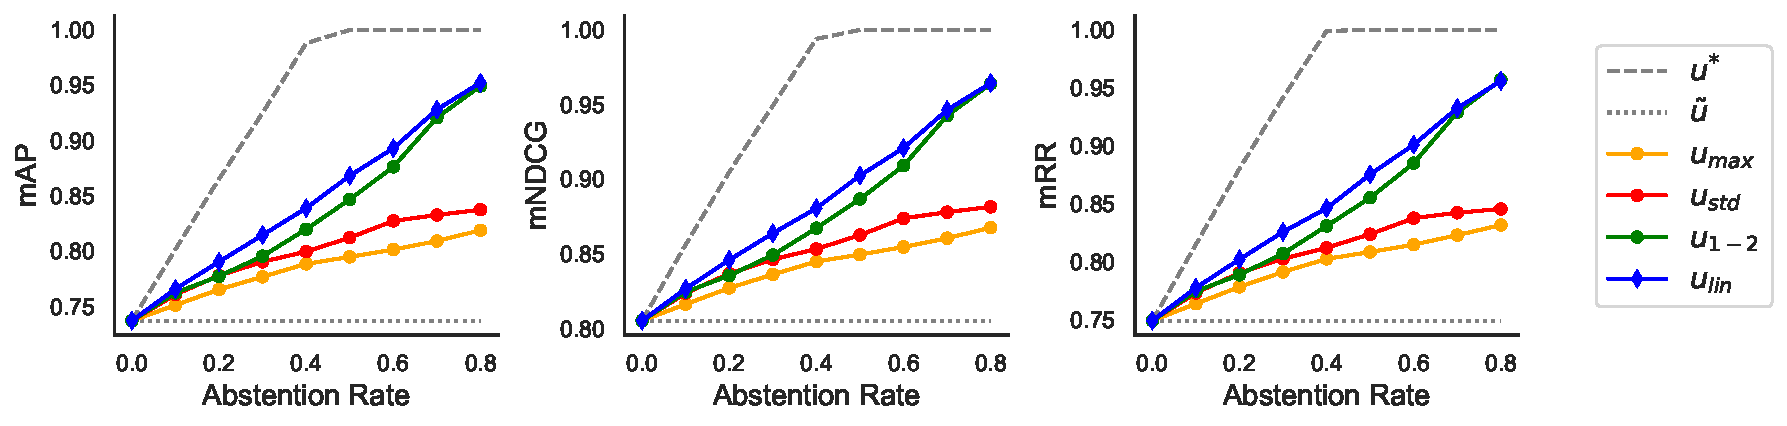
\includegraphics[width=0.9\textwidth]{images/reranking_figures/perf_vs_abst.pdf}
% \vspace{-5mm}
% % \captionof{figure}{Performance-abstention curves for the \texttt{ember-v1} model on the \textsc{StackOverflow} dataset. All methods show increasing curves, indicating effective abstention. The reference-based method, $u_{\text{lin}}$, stands out above the others, demonstrating superior abstention performance. Note that $u^*$ and $\tilde{u}$ respectively denote the oracle and the random baseline, associated with the $\rho^*$ and $\tilde{\rho}$ mechanisms (Sections \ref{sec:abst_pb} and \ref{sec:ass_abst_perf}).}
% \label{fig:perf_vs_abst}

% \end{figure}

% We report nAUC (Equation \ref{eq:nauc}) for all methods described in Section \ref{sec:conf_assess}, averaged model-wise (Table \ref{tab:naucs}), and illustrate the dynamics of the performance-abstention curves for the \texttt{ember-v1} model on the \textsc{StackOverflow} dataset in Figure \ref{fig:perf_vs_abst}.

% \noindent \textbf{Abstention works.} All evaluated abstention-based methods improve downstream evaluation metrics (nAUCs greater than 0), showcasing the relevance of abstention approaches in a practical setting.

% \noindent \textbf{Reference-based abstention works better.} The value of reference-based abstention approaches is demonstrated in Table \ref{tab:naucs}, in which we notice that the linear-regression-based method  $u_{\text{lin}}$ performs on average largely better than all reference-free baselines, edging out the best baseline strategy ($u_{\text{std}}$) by almost 10 points on the mAP metric.

% Having shown the superiority of reference-based abstention methods across the entire benchmark, we conduct (unless otherwise specified) the following experiments on the \texttt{ember-v1} model using mAP for evaluation (main metric in the MTEB leaderboard \sidecite{muennighoff2022mteb}), and compare $u_{\text{lin}}$ to $u_{\text{std}}$, respectively the best reference-based and reference-free methods mAP-wise.

% \subsection{Abstention Effectiveness vs. Raw Model Performance}
% \label{sec:abstperf_vs_perf}

% \begin{figure}[t]
% \centering
% \begin{minipage}{0.5\textwidth}
% \centering
% 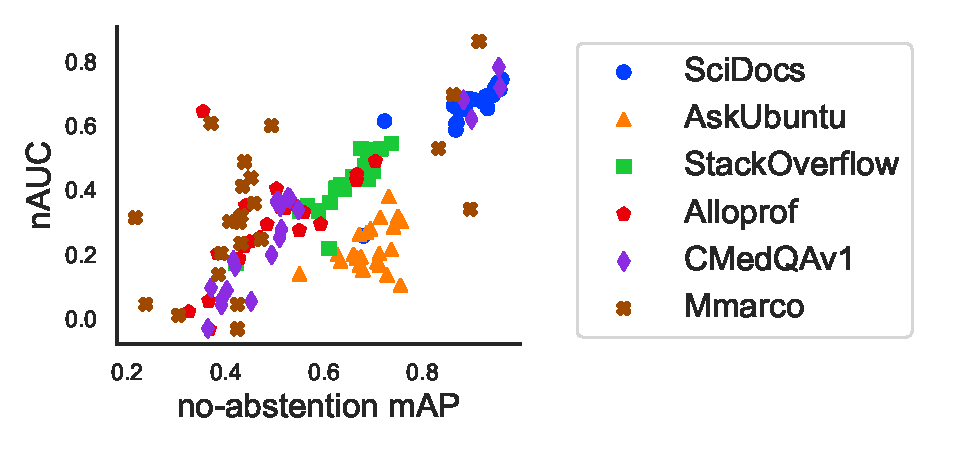
\includegraphics[width=0.98\linewidth]{images/reranking_figures/abstperf_vs_perf.pdf}
% \vspace{-5mm}
% % \captionof{figure}{Abstention performance (nAUC in \%) vs. no-abstention performance (mAP), for all models and datasets, using $u_{\text{lin}}$ as a confidence function. Each data point represents a model-dataset pair.}
% \label{fig:abstperf_vs_perf}
% \end{minipage}
% \hspace{5mm} % Add horizontal space between minipages
% \begin{minipage}{0.4\textwidth}
% \centering\small
% % \captionof{table}{Pearson's correlations between no-abstention mAP and abstention nAUC, for each dataset. General correlation is computed over the whole scatter plot, i.e., across all dataset-model pairs.}

% \vspace{2mm}
% \resizebox{0.57\textwidth}{!}{\begin{tabular}{lc}
% \toprule
% \textbf{Dataset} & \textbf{Correlation} \\
% \midrule
% \textsc{SciDocs} & 0.85 \\
% \textsc{AskUbuntu} & 0.38 \\
% \textsc{StackOverflow} & 0.90 \\
% \textsc{Alloprof} & 0.56 \\
% \textsc{CMedQAv1} & 0.94 \\
% \textsc{Mmarco} & 0.63 \\
% \midrule
% \textbf{General} & \textbf{0.73} \\
% \bottomrule
% \end{tabular}}
% \label{tab:abstperf_vs_perf}
% \end{minipage}
% \end{figure}


% We investigate whether a correlation exists between abstention effectiveness and model raw performance (i.e., without abstention) on the reranking task. For each model-dataset pair, we compute both no-abstention mAP and abstention nAUC, using $u_{\text{lin}}$ as a confidence function (Figure \ref{fig:abstperf_vs_perf}, Table \ref{tab:abstperf_vs_perf}).

% \noindent \textbf{A better ranker implies better abstention.} Figure \ref{fig:abstperf_vs_perf} and Table \ref{tab:abstperf_vs_perf} showcase a clear positive correlation between model raw performance and abstention effectiveness, albeit with disparities from one dataset to another. Better reranking methods naturally produce more calibrated score distributions, which in turn leads to improved abstention performance. This highlights the value of incorporating abstention mechanisms into high-performing retrieval systems and reinforces that their purpose is not to turn weak rankers into strong ones, but to enhance the quality of models that already perform reasonably well. For thoroughness, we evaluated a range of open-source models with varying performance levels, though in practice, users typically select models they already know to be sufficiently effective.

% \subsection{Threshold Calibration}
% \label{sec:threshold_calibration}



% \begin{figure}[t]
% \centering
% \begin{minipage}[t]{0.5\textwidth}

% % \captionof{table}{MAEs for target vs. achieved abstention rates and performance levels (in \%) (model: \texttt{ember-v1}, dataset: \textsc{StackOverflow}, metric: mAP).}
% \label{tab:calib}
% \centering \small
% \vspace{2mm}
% \resizebox{0.95\textwidth}{!}{\begin{tabular}{lclll}
% \toprule
%  & \textbf{Target Abstention} & 10\% & 50\% & 90\% \\
% \midrule
% \multirow[t]{2}{*}{\textbf{Rate}} & $u_{\text{std}}$ & 1.10 & 1.80 & 1.08 \\
%  & $u_{\text{lin}}$ & 1.07 & 1.79 & 1.09 \\
% \cline{1-5}
% \multirow[t]{2}{*}{\textbf{mAP}} & $u_{\text{std}}$ & 1.24 & 1.52 & 3.09 \\
%  & $u_{\text{lin}}$ & 1.22 & 1.33 & 1.51 \\
% \bottomrule
% \end{tabular}}
% \end{minipage}
% \hspace{5mm} % Add horizontal space between minipages
% \begin{minipage}[t]{0.4\textwidth}
% %\captionof{table}{nAUCs averaged test-set-wise (model: \texttt{ember-v1}, metric: mAP).}
% \label{tab:transfer}
% \small
% \centering
% \vspace{2mm}
% \resizebox{0.785\textwidth}{!}{\begin{tabular}{lllll}
% \toprule
% \multicolumn{1}{r}{\textbf{Method}} & $u_{\text{max}}$ & $u_{\text{std}}$ & $u_{\text{1-2}}$ & $u_{\text{lin}}$ \\
% \textbf{Reference set} & & & & \\
% \midrule
% \textsc{Alloprof} & 30.1 & \textbf{32.7} & 17.1 & 31.4 \\
% \textsc{AskUbuntu} & 28.5 & 32.1 & 19.8 & \textbf{34.2} \\
% \textsc{CMedQAv1} & 27.9 & 31.1 & 17.2 & \textbf{34.2} \\
% \textsc{Mmarco} & 27.5 & \textbf{32.2} & 18.9 & 34.9 \\
% \textsc{SciDocs} & 23.0 & \textbf{23.5} & 22.3 & 11.6 \\
% \textsc{StackOverflow} & 29.3 & \textbf{30.7} & 11.9 & 20.6 \\
% \hline
% \textbf{Average} & 27.7 & \textbf{30.4} & 17.9 & 27.8 \\
% \bottomrule
% \end{tabular}}
% \end{minipage}
% \end{figure}

% In practical industrial settings, a major challenge with abstention methods lies in choosing the right threshold to ensure a desired abstention rate or performance level on new data. To evaluate threshold calibration quality, we choose three target abstention rates (10\%, 50\%, and 90\%) and rely on the reference set\sidenote{In this setting, access to a reference set is essential in order to determine which threshold value corresponds to a given abstention rate or level of performance.} to infer the corresponding threshold and level of performance (here, the mAP). Then, the Mean Absolute Error (MAE) between target and achieved values on test instances is reported (Table \ref{tab:calib}), averaging across 1000 random seeds on the \textsc{StackOverflow} dataset.\sidenote{For example, if the mAP corresponding to a target abstention rate of 50\% in the reference set is 0.6 and the values achieved on test set on 2 different seeds are 0.5 and 0.7, the MAE is be equal to $1/2 \times (|0.6 - 0.5| + |0.6 - 0.7|) = 0.1$.}

% \noindent \textbf{$u_{\text{lin}}$ is better calibrated than $u_{\text{std}}$.} The lower part of Table \ref{tab:calib} shows that the MAE between the target and achieved mAP increases with the abstention rate, which is logical because a higher abstention rate reduces the number of evaluated instances and therefore increases volatility. However, we observe that the MAE increases much less significantly for the $u_{\text{lin}}$ method than for the $u_{\text{std}}$ method, with the latter having a MAE twice as high at a target abstention rate of 90\%. This provides strong evidence that $u_{\text{lin}}$ is more reliable at high abstention rates.


% \subsection{Domain Adaptation Study}
% \label{sec:dom_adap}

% In a practical setting, it is rare to have a reference set that perfectly matches the distribution of samples seen at test time. To measure the robustness of our method to data drifts, we fit them on a given dataset and evaluate on all others.

% \noindent \textbf{Reference-based approaches are globally not robust to domain changes.} From Table \ref{tab:transfer}, we see on average that the reference-based method underperforms reference-free baselines when fitted on the "wrong" reference set. However, certain reference datasets seem to enable methods to generalize better overall, even out of distribution, which is mainly an artifact of the number of positive documents per instance (further insights in Appendix \ref{ap:dom_adap}).

% \subsection{Reference Set Minimal Size}

% \begin{figure*}[t]
% \centering
% \begin{minipage}{0.36\textwidth}
% \centering\small
% \vspace{-3mm}
% % \captionof{table}{Minimum reference set size for $u_{\text{lin}}$ to outperform $u_{\text{std}}$ (model: \texttt{ember-v1}, metric: mAP).}
% \vspace{2mm}
% \label{tab:ref_size}
% \resizebox{0.9\textwidth}{!}{\begin{tabular}{lc}
% \toprule
% \textbf{Dataset} & \textbf{Break-Even} \\
% \midrule
% \textsc{SciDocs} & 12 \\
% \textsc{AskUbuntu} & 9 \\
% \textsc{StackOverflow} & 19 \\
% \textsc{Alloprof} & 58 \\
% \textsc{CMedQAv1} & 50 \\
% \textsc{Mmarco} & 80 \\
% \hline
% \textbf{Average} & \textbf{38} \\
% \bottomrule
% \end{tabular}}

% \end{minipage}

% \hspace{5mm} % Add horizontal space between minipages
% \begin{minipage}{0.54\textwidth}

% \centering
% 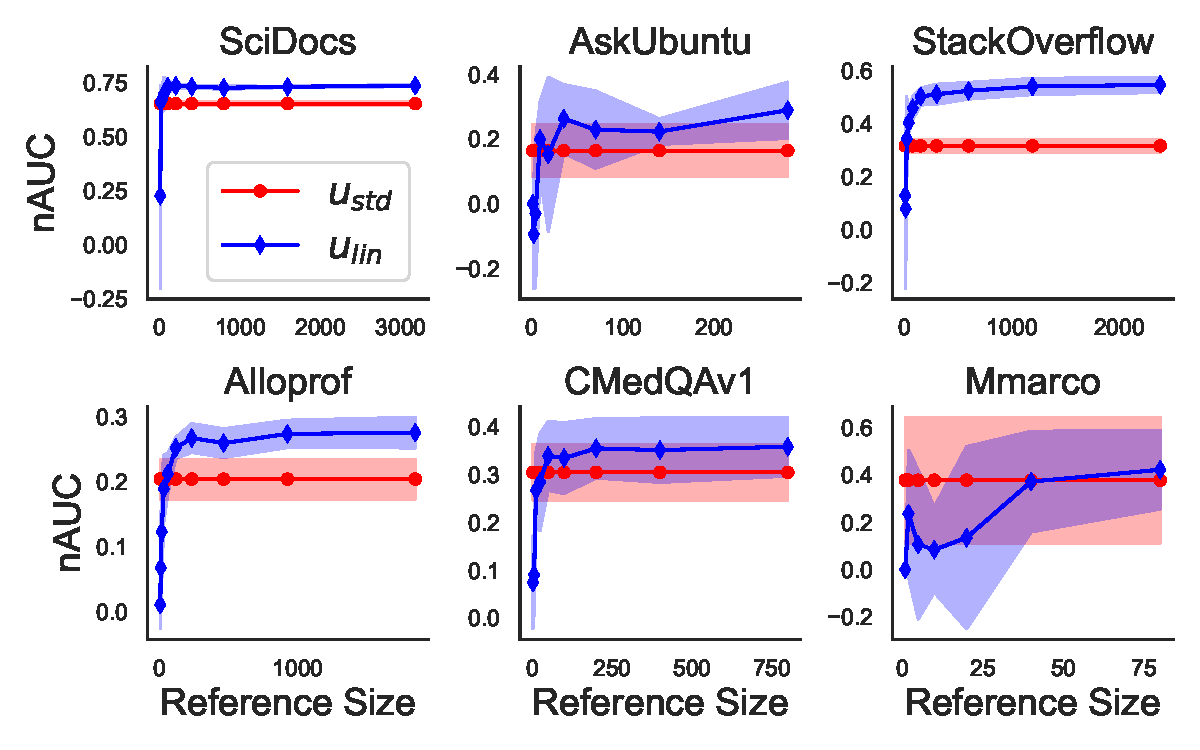
\includegraphics[width=0.8\textwidth]{images/reranking_figures/ref_size.pdf}
% \vspace{-5mm}
% % \captionof{figure}{nAUC vs. reference set size for $u_{\text{lin}}$ and $u_{\text{std}}$ on all datasets (model: \texttt{ember-v1}, metric: mAP).}
% \label{fig:ref_size}

% \end{minipage}
% \end{figure*}


% Calibrated reference-based methods outperform reference-free baselines (Section \ref{sec:abst_perf}) but require having access to an in-domain reference set (Section \ref{sec:dom_adap}). To assess the efforts required for calibrating these techniques to extract best abstention performance, we study the impact of reference set size on method performance.

% \noindent \textbf{Small reference sets suffice.} From Figure \ref{fig:ref_size} and Table \ref{tab:ref_size}, we note that $u_{\text{lin}}$ requires only a fairly small amount of reference data (less than 40 samples on average) to outperform $u_{\text{std}}$, which demonstrates the effectiveness of using a reference set even when data is scarce. This provides strong evidence on the applicability of our method to practical industrial contexts, the labeling of around 50 samples appearing perfectly tractable in such settings.

% \subsection{Computational Overhead Analysis}

% \begin{figure}[t]
% \centering
% \begin{minipage}{0.36\textwidth}
% 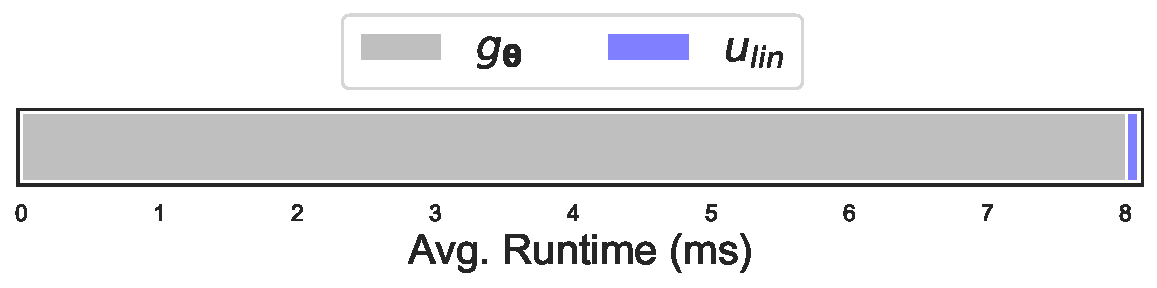
\includegraphics[width=\linewidth]{images/reranking_figures/runtime.pdf}
% \end{minipage}
% \hspace{5mm} % Add horizontal space between minipages
% \begin{minipage}{0.54\textwidth}
% \vspace{-3mm}
% \caption{Comparison between relevance ($g_{\bm{\theta}}$) and confidence ($u_{\text{lin}}$) assessment times on one Apple M1 CPU (model: \texttt{all-MiniLM-L6-v2}, dataset: \textsc{StackOverflow}).}
% \label{fig:runtime}
% \end{minipage}
% \end{figure}

% Crucial to the adoption of our abstention method is the minor latency overhead incurred at inference time. In our setup, we consider documents are pre-embedded by the bi-encoders, and stored in a vector database. We average timed results over 100 runs on a single instance prediction, running the calculations on one Apple M1 CPU (Figure \ref{fig:runtime}). To upper-bound the abstention method overhead, we baseline the smallest model with the fastest embedding time available (\texttt{all-MiniLM-L6-v2}).

% \noindent \textbf{Our data-based abstention method is free of any significant time overhead.} $u_{\text{lin}}$-based confidence estimation accounts for only 1.2\% of relevance scores calculation time (Figure \ref{fig:runtime}), making it an almost cost-free option.\sidenote{If we used a cross-encoder, documents could not be pre-embedded as they need to be appended to the input query. In that scenario, the computation time required for $g_{\bm{\theta}}$ would therefore increase, while that required for $u_{\text{lin}}$ would remain unchanged, thus reducing the relative extra running time.}


\section{Conclusion}

We developed a lightweight abstention mechanism tailored to real-world constraints, agnostic to the ranking method and shown to be effective across various settings and use cases. Our method, which only requires black-box access to relevance scores and a small reference set for calibration, is essentially a free-lunch to plug to any retrieval system, in order to gain better control over the whole IR pipeline. 

% \setchapterpreamble[u]{\margintoc}
\chapter{Trustworthiness Through Evaluation}
% \chapter{Revisiting Instruction Fine-tuned Model Evaluation to Guide Industrial Applications}


\begin{kaobox}[frametitle=Paper Abstract]

Instruction Fine-Tuning (IFT) is a powerful paradigm that strengthens the zero-shot capabilities of Large Language Models (LLMs), but in doing so induces new evaluation metric requirements. We show LLM-based metrics to be well adapted to these requirements, and leverage them to conduct an investigation of task-specialization strategies, quantifying the trade-offs that emerge in practical industrial settings. Our findings offer practitioners actionable insights for real-world IFT model deployment.
\end{kaobox}


\section{Introduction}
\label{sec:introduction}

Adapting pre-trained language models (LMs) for specific applications is central in industrial NLP to unlock task-specific performance gains and strengthen model alignment with industry requirements.  A paradigm gaining traction is the use of instruction fine-tuned (IFT) models, LMs capable of following arbitrary instructions expressed in natural language \sidecite{wei2022finetuned, sanh2022multitask, ouyang2022training}.

Researchers primarily concentrate on improving general-purpose IFT models to be used as versatile agents capable of executing instructions expressed in natural language \sidecite{li2023camel, zhou2023lima, xu2023wizardlm}. 
In an industrial setting, prompting ChatGPT to improve the wording of an email, or to assist with a code snippet would be instances of this zero-shot utilization scenario, which we define as $\mathcal{S}_0$. 
Critical industrial LLM applications may however not always align with $\mathcal{S}_0$, and often prioritize two other settings. The first scenario, $\mathcal{S}_1$, requires extending a generalist IFT model's capabilities to new specific tasks not included in the original instruction training set. The second scenario, $\mathcal{S}_2$, centers around converting IFT models into specialized models proficient \emph{exclusively} on specific tasks.  
%In $\mathcal{S}_1$, the aim is to obtain an IFT model that retains its zero-shot abilities on arbitrary tasks, but has improved abilities on newly introduced tasks tailored to usage-specific needs. 
%
In $\mathcal{S}_1$ for instance, a large company may want an LLM assistant for internal employee use, and decide to extend an openly available Chat model by training it to write memos with a specific templating scheme, to respond to internal FAQs, and to use internal coding tools, all the while retaining the original chat assistant's general purpose abilities. In $\mathcal{S}_2$, that same company is only interested in a given specific task; extracting specific information from business documents, and specializes an IFT model for that purpose, aiming to leverage prompting and the generalization capabilities of the model for a more data-efficient training.

% %Formally our contributions are:
% In this paper, we thoroughly examine $\mathcal{S}_1$ and $\mathcal{S}_2$ through a practical lens. As a starting point, we undertake a critical assessment of the current evaluation practices employed for IFT models to ensure the reliability of our conclusions. 
In this paper, we thoroughly examine $\mathcal{S}_1$ and $\mathcal{S}_2$ by investigating the learning dynamics of specializing IFT models through a practical lens. To ensure the reliability of our tooling and the rigor of our conclusions, we first undertake a critical assessment of the current evaluation practices employed for IFT models. Formally, our contributions are:

\noindent\textbf{Contribution 1.} IFT models are designed to handle tasks of diverse natures and varying difficulties. However, current metrics used to measure their performance are often task-specific \sidecite{zellers2019hellaswag, eval-harness}, or rely on automatic metrics designed for other intended purposes \sidecite{papineni-etal-2002-bleu, lin-2004-rouge}. To address this limitation, we introduce two new requirements for metrics used to evaluate IFT models: \underline{C}omparability \underline{A}cross \underline{T}ask (\texttt{CAT}) and \underline{T}ask and \underline{F}ormat \underline{A}gnostism (\texttt{TFA}). \texttt{CAT} imposes for metric scores to exhibit consistency across a diverse set of generative tasks, in contrast to the sole traditional focus of consistency within a specific task. \texttt{TFA} defines the need for metrics to demonstrate robustness to variations in the output formats. By highlighting the shortcomings of existing metrics in meeting \texttt{CAT} and \texttt{TFA}, we present compelling evidence that using LLMs as scoring agents is a viable evaluation alternative of IFT models. 

\noindent\textbf{Contribution 2.} We approach our examination of $\mathcal{S}_1$ and $\mathcal{S}_2$ from a practical perspective and focus on the trade-off between data availability and overall performance. Our analysis uncovers two distinct phases of learning during IFT model specialization: learning to format, and learning to solve tasks. Subsequently, we showcase how practitioners can (i) leverage synthetic data to facilitate learning the desired formatting aspects and (ii) use IFT models to reduce the need of expert data in industrial scenarios. Our study provides practical insights and actionable recommendations to practitioners looking to deploy IFT models in production settings.\sidenote{Code and evaluation datasets are available on \url{https://github.com/ManuelFay/IFTEval}.}

\section{Re-evaluating IFT Model Evaluation}

% \subsection{Need for New Evaluation Requirements}
\subsection{What Should Good Scorers Measure?}
\label{sec:evalreq}
In scenarios $\mathcal{S}_0$, $\mathcal{S}_1$, and $\mathcal{S}_2$, IFT models are trained to perform generative tasks. Unlike models designed for single tasks with known output formats, IFT models have the capacity to generate diverse valid responses across different tasks and formats \sidecite{ouyang2022training}. The novel capabilities of IFT models impose new considerations when selecting an automatic evaluation metric. 
\\\noindent \textbf{Comparability across tasks (\texttt{CAT}).}
Standard evaluation metrics aim to fulfill one key requirement: coherence within each task with respect to human judgment \sidecite{specia2010machine}. However, due to the multi-task nature of IFT models, the scores should also be comparable across different tasks \sidecite{colombo2022best,himmi2023towards}. In other words, the scoring scale should be absolute and coherent with human preferences on all tasks. To measure the \texttt{CAT} we will mix samples of different tasks and compute the Spearman correlation ($\rho$) of their score with human judgment\sidenote{Common when benchmarking metrics \cite{bhandari-etal-2020-evaluating,colombo2021automatic,chhun2022human,staerman2021pseudo, fabbri-etal-2021-summeval,colombo2021automatic}, we extend the tool to inter-task settings.}. 
This requirement is essential in scenarios $\mathcal{S}_0$ and $\mathcal{S}_1$ to measure model performance across different tasks, and make informed decisions regarding the trade-offs between model variants.
\\\noindent \textbf{Task and Format-Agnostism (\texttt{TFA}).} Evaluation metrics should be robust to artifacts associated with the output format and to the nature of the evaluated task \sidecite{liang2022holistic}. Implementing task-specific scoring metrics is not a scalable solution for generalist IFT models. To measure \texttt{TFA}, we compute the relative target task improvement between models prompted in a zero-shot manner and models that mastered the task format (trained on 1000 target task samples). Comparing each metric's \texttt{TFA} to human-reported performance improvements allows to grasp the extent to which mastery of the task format influences the metric performance, independently of intrinsic task performance.
 In industrial scenarios, this requirement is essential as it ensures minimal bias in the evaluation due to training data formatting artifacts. In practice, many datasets that industrial actors may add to the training instruction set ($\mathcal{S}_1$), or fully train a model on ($\mathcal{S}_2$) have specific response formatting that differs from what a zero-shot model will answer, leading to a potentially large formatting bias.

\noindent\textbf{Comparability intra-task (\texttt{CIT}).} While in no way a novel requirement, it is essential for metrics to measure performance consistently within a given task.  We verify this by computing the Spearman $\rho$ correlation coefficient between samples of a specific task and human judgments.

In all industrial scenarios for IFT LLMs, rigorous model evaluation is necessarily linked to evaluation metrics that comply with both \texttt{CAT} and \texttt{TFA}, as well as the standard \texttt{CIT} measures.

\subsection{Existing Metrics}
\textbf{Current Evaluation.} Currently, two dominant paradigms emerge for assessing the performance of IFT models: (i) relying on reference-matching scoring metrics such as \texttt{ROUGE-L} \sidecite{lin-2004-rouge}, or normalized log-probabilities of class labels in few-shot classification benchmarks \sidecite{hendrycks_measuring_2020, eval-harness, zellers2019hellaswag}, and (ii) model ranking frameworks, based on pairwise preference comparisons of response quality judged by humans or LLM evaluators \sidecite{vicuna2023, dubois2023alpacafarm, gudibande2023false}. Language Model based scoring has been shown to be a promising alternative on specific tasks, such as summarization \sidecite{liu2023geval,colombo2022infolm} or translation \sidecite{kocmi2023large, xu2023instructscore}. Our work extends these findings to showcase the multi-task scoring capabilities of LLMs with respect to \texttt{CAT} and \texttt{TFA}.

\noindent\textbf{LMs as Viable Scoring Mechanisms.} 
Given the inherently open nature of IFT model generation, we adopt a reference-free setting to ensure unbiased evaluation. We present an input prompt and the corresponding generated response to the LLM\footnote{We rely on LMs available through the OpenAI API (\textit{i.e.}, GPT4 and GPT3.5). See \autoref{sec:metrics} for details.}, prompting it to assign a score on a scale of 0 to 10, subsequently scaling it between 0 and 1 to facilitate comparisons with other evaluation metrics. % Concurrent works in the literature employ similar methods.

\noindent \textbf{Baseline Metrics.}  We assess the fulfillment of both \texttt{CAT} and \texttt{TFA} by comparing the proposed metrics against well-established \textit{reference-based} metrics, including ROUGE\footnote{ROUGE-1 is used here, it is best on one-word long labels}, BScore \sidecite{zhang2020bertscore}, and SBERT \sidecite{reimers2019sentencebert}, as well as a \textit{machine learned} metric, the OpenAssistant Reward Model (RM) \sidecite{köpf2023openassistant} trained on human preferences. 

\begin{figure*}[ht]
\begin{minipage}{.95\textwidth}
\centering
    % \captionof{table}{\emph{(Left)} \textbf{$\rho$ correlation between human scores and metrics} on the summarization task (SUM), on the \emph{human data} tasks individually then averaged in (CIT), and on the concatenated human tasks (CAT) to form inter-task settings. (TFA) denotes relative metric improvement after 1000 target task samples are added to the training set. \emph{(Right)} \textbf{Metric scores} averaged per \emph{synthetic data} category}\vspace{-.3cm}
    \begin{minipage}{.45\textwidth}
      \centering
      \tiny
      \label{tab:main_metrics}
\resizebox{\textwidth}{!}{\begin{tabular}{lrrrr}
    \toprule
     Scorers & SUM & CAT &  CIT & TFA \\ %TFA $\Delta$ CIT\
    \midrule
    ROUGE & 0.28 & 0.22 & 0.57 & +513.9 \% \\
    BScore & 0.21 & 0.22 & 0.13  & +49.0 \% \\
    SBERT & 0.25 & 0.29 & 0.43 & +86.3 \% \\
    % RM (*) & 0.24 & 0.03 & 0.25  & N/A \\
    RM & 0.20 & 0.28 & 0.29 & -44\% \\
    \hline
    GPT4 & \textbf{0.45} & \textbf{0.68} & \textbf{0.77} & +2.1 \% \\
    GPT-3.5 & 0.42 & -0.19 & 0.48  & +9.5 \% \\
    \hline
    Human & 0.54 & - & - & +12.0 \% \\
    \bottomrule
    \end{tabular}}
    \end{minipage}\hspace{-.2cm}
    \begin{minipage}{.55\textwidth}
      \centering
        \tiny
            \resizebox{0.92\textwidth}{!}{\begin{tabular}{lrrrrrrr}
    \toprule
    Scorers & Logic & Code  & Memory & Write \\
    \midrule
     ROUGE & \textbf{0.52} & 0.46 & 0.47 & \textit{0.41} \\
     BScore & \textbf{0.73} & \textit{0.71} & \textbf{0.73} & 0.72 \\
     SBERT & 0.80 & 0.74  & \textbf{0.84} & \textit{0.74} \\
     % RM  & 0.33 & 0.73 & -0.20 & 1.61 & 2.78 & 3.21 \\
     RM & \textbf{0.49} & 0.43 & \textit{0.28} & 0.33 \\
     \hline
     GPT4 & \textit{0.71} & 0.79  & 0.93 & \textbf{0.97} \\
     GPT-3.5 & \textbf{0.88} & \textit{0.82} & 0.87 & 0.86 \\
    \bottomrule
    \end{tabular}}
    \end{minipage} \hfill
\end{minipage}
    \begin{minipage}{.28\textwidth}
    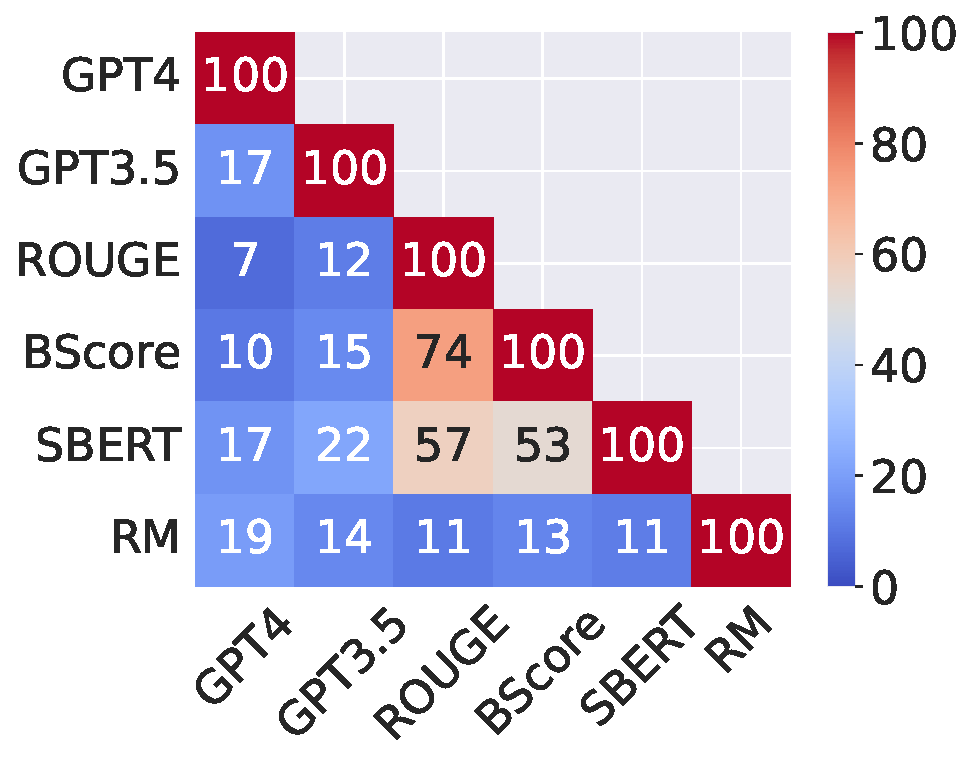
\includegraphics[width=\textwidth]{images/learning_dynamics/exp1a_corr.pdf}
    % \captionof{figure}{\textbf{Spearman $\rho$ between metrics} on synthetic data.}
    \label{fig:correlations}
    \end{minipage}
\end{figure*}
\subsection{Experimental setup}

\textbf{Training an IFT model.} IFT models are trained by fine-tuning a base model on a large instruction corpus, collected either through human annotations \sidecite{ouyang2022training, köpf2023openassistant} or concatenating task-specific datasets \sidecite{sanh2022multitask, mishra2022crosstask}. In line with recent work \sidecite{vicuna2023,wang2023selfinstruct,peng2023instruction}, we leverage synthetic data as the base instruction set in our IFT models \sidecite{alpaca2023}.
% Motivated by real-world industrial applications where cost is a primary concern, we rely on synthetic datasets to train the base IFT model.


\noindent\textbf{Benchmarking automatic metrics.} To benchmark the metrics, we rely on a combination of synthetic and real data.  For \emph{synthetic data}, we use the Alpaca GPT4 dataset \cite{alpaca2023}, and tag the data in 13 task categories (see \autoref{sec:alpaca-pres}) (\textit{e.g.}, logic, code, rewrite).  For \emph{human data}, we focus on tasks with industrial interests. Specifically, we include Natural Language Inference \sidecite{N18-1101, wang2019glue}, Question Answering \sidecite{rajpurkar2016squad}, NER \sidecite{tjong-kim-sang-de-meulder-2003-introduction}, and Sentiment Classification \sidecite{socher2013recursive, agirre-etal-2013-sem}). To build our metric evaluation dataset, we train and run LLaMA-7B models \cite{touvron2023llama} on varied data mixtures and target tasks. For rigor, we also report scores on the summarization with human feedback dataset from \sidecite{stiennon2022learning} (\texttt{SUM}).\sidenote{More details in \autoref{sec:exp_setup_1})}


\subsection{Experimental results}
To better understand the limitation of existing metrics we conduct both single-task analysis to ensure that metrics are able to score tasks reliably as well as multi-task analysis, which is the standard setting for IFT models. Results are reported in Tab. \ref{tab:main_metrics}.
% Insert table with checks or not

\noindent\textbf{\texttt{CIT} Analysis.} From Tab. \ref{tab:main_metrics}(left, \texttt{SUM}), we observe that the average correlation with human scores for evaluated summaries are higher for LLM models than with traditionally used metrics. Intra-task correlations on all other \emph{human data} tasks, averaged in \texttt{CIT} lead to similar conclusions. 


\noindent\textbf{\texttt{CAT} Analysis.} Tab. \ref{tab:main_metrics}(left) shows that all metrics, \emph{with the exception of the GPT4-based metric}, exhibit weak or no correlation in the context of inter-task consistency. While it is true that existing metrics demonstrate the ability to differentiate between good and bad samples within a single task (\texttt{CIT}), their \emph{performance falls short when confronted with the open setting imposed by IFT models}.
% here we could mention GPT3 bad results on CAT (see comment thread)
%u: très mal calibré sur de l inter taches, d autres scorers donnaient aussi des resultats negatifs ou nuls qu on a enlevé petit a petit, ca parait effectivement plus choquant mtn que les autres sont à ~20%il est aussi reference-free ce qui l handicappe intrinsequement sur des taches du genre, c est une conclusion qu on avaitmise a un moment, que le modele LLM de scoring se devait d etre bon en soit sur la tache en question pour avoir une chance


% Express 
\noindent\textbf{\texttt{TFA} Analysis.} On non-LLM-based metrics, performance gains reported between zero-shot models, and models trained on 1000 target-task samples (Tab. \ref{tab:main_metrics}(left), \texttt{TFA}) largely exceed the  12.0 \% relative improvement of human scores, and demonstrate how format, once learned, unrealistically boosts reference-based metrics which are heavily impacted by format.

\noindent\textbf{Metric Similarity Analysis.} \autoref{fig:correlations} displays metric correlation at the sample level on the synthetic dataset. The results align with \sidecite{chen2022reproducibility}, indicating a moderate to high correlation between BERT-based metrics and ROUGE-L. However, all metrics exhibit a low correlation with GPT4, indicating different response features are scored. 

\noindent\textbf{Zoom on GPT4.} Tab.\ref{tab:main_metrics}(right) shows a strong correlation between the results of GPT4-based metrics and the corresponding LLM task abilities reported in \sidecite{wei2022emergentabilitieslargelanguage} (Logic and Coding are non-trivial for LLMs, Writing tasks are relatively easier). However, reference-based metrics such as ROUGE suggest the opposite, as they are biased by the high syntactic overlap between model outputs and reference answers in these categories. The GPT3.5 scorer also highly rates results on the Logical Reasoning tasks, contrarily to GPT4. This is due to its lesser ability to spot logical inconsistencies in the evaluated responses \sidecite{bubeck2023sparks}, hinting that evaluator models must be capable at the evaluated task themselves in order to produce meaningful scores.

% \autoref{tab:main_metrics}(right) illustrates the importance of a unified scale across different tasks (as illustrated by automatically tagged classes such as logic, code, rewrite). We observe that the results of GPT4 correlate with related weaks and we found that some tasks (Logic) also require strong task abilities while task such as rewrite are easier. By considering other metrics such as ROUGE tge results is less clear (extract is harder that rewrite).


Our findings highlight the inadequacy of existing metrics in quantifying the performance of IFT models, while emphasizing GPT4 as a promising candidate. This performance gap in evaluation capabilities is primarily explained by GPT4's reduced dependence to reference answers, leading to a more coherent and absolute evaluation scale \texttt{CAT}, and an improved robustness to variations in output formatting \texttt{TFA}. \emph{The GPT4 scorer's powerful capabilities unlock the study of novel settings traditional metrics would struggle with} \sidecite{schaeffer2023emergent}.
% \emph{We find GPT4 to be a powerful scorer, unlocking the study of novel settings traditional metrics would struggle with.} \sidecite{schaeffer2023emergent}


\section{IFT Models for Industrial Applications}% Limits of evaluation metrics}
% \input{setup.tex}


\subsection{$\mathcal{S}_1$: Improving Specific Tasks}\label{ssec:scenario1}
In this section, we delve into $\mathcal{S}_1$, which specifically aims to extend an IFT model's capabilities to better perform on specific instructions.
%Motivated by industrial considerations, our goal is to assess the trade-off between data and quality in the performance of the final task.

%(i) How many samples are needed for a general-purpose model to "learn" a new task? (ii) Is learning an output format disentangled from improving the model's zero shot capacities on the task itself? (iii) Does learning a new task degrade the model's performance across other tasks?

\noindent\textbf{Setting.} We fine-tune a base 7B-LLM model (Pythia \sidecite{biderman2023pythia}, Bloom \sidecite{scao2022bloom}, Falcon \sidecite{penedo2023refinedweb}, or LLaMA) using synthetic instructions. In each training iteration, we introduce a selected number of $N$ \emph{real} target task samples into the synthetic dataset. We evaluate the model performance on an independent test subset of the target task. More experimental details are given in \autoref{sec:exp_setup_app_31}.
% These tasks are adapted from non-generative benchmarks and have been formatted to be processed by a generative LLM.
\begin{figure}[ht]
    \centering
    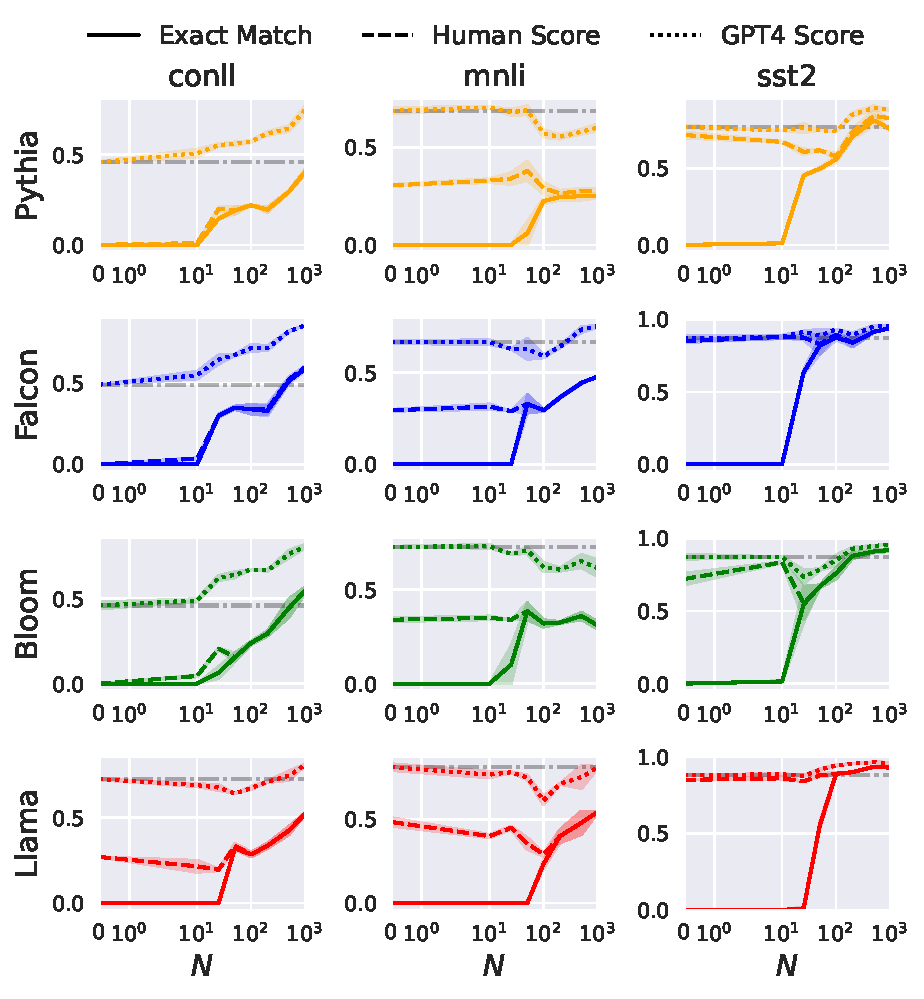
\includegraphics[width=0.8\textwidth]{images/learning_dynamics/exp1b_all.pdf}
    \caption[IFT training with real samples]{Incorporating $0 \leq N \leq 1000$ real task samples into IFT model training}
    \label{fig:exp1b_all}
\end{figure} %  N in \{10,50,100,200, 500,1000\}

\noindent\textbf{Mastering Format to Foster Understanding.} \autoref{fig:exp1b_all} shows target task performance as the number of target task samples introduced within the base training set increases. Across all tasks and models, \emph{specialization is biphasic}: first, \textit{task output format} is learned while overall performance remains constant, or even slightly decreases. Only once the format has been mastered, as noted by the spike of the Exact Match, does the model improve upon its \textit{underlying task performance} (Human and GPT4 scores increase), eventually surpassing the original zero-shot performance. It is worth noting that this analysis is made possible by format-agnostic scorers (\texttt{TFA}) that can accurately decouple output format from underlying model performance.

\noindent\textbf{Measuring Model Forgetting.} Performance on a test split of the Alpaca data shows little to no performance degradation (<1\%) caused by the inclusion of new tasks to the training mix (\autoref{sec:app_perf_deg}).


% \noindent \textbf{Harnessing Synthetic Datasets for Formatting Mastery} 
\noindent \textbf{Leveraging Synthetic Data to Learn to Format.} Our findings suggest a straightforward approach to optimizing the use of real examples: \emph{employ synthetic examples to assist the model in mastering the desired format before relying on real samples to enhance overall model performance}. We repeat the previous experiment, replacing the $N$  human-annotated target task training samples (\emph{H}), by GPT4 synthetically-generated samples  (\emph{S}), or synthetic samples with random labels (\emph{R}) (\autoref{fig:random}) \texttt{Exact Match} shows synthetic or randomly labeled data can indeed be used to learn the desired format, although the better quality human data eventually yields better results with more samples. In (\emph{S+H}), we train on 100 synthetic samples, then on $N$ human-annotated samples. This technique enables the model to master the format before being trained on high-quality data, largely improving human annotated data sample efficiency.
% However, comparable outcomes and more efficient learning can be attained by combining both \emph{synthetic} and \emph{human} datasets. As expected, clear performance degradation is seen in the Random setting past a certain number of samples.
%\emph{We can thus train our models to learn format on synthetic or low-quality data, to improve sample efficiency once training with real data !}

%A follow-up experiment displayed in Figure \ref{fig:random}, consists of replacing the target task by respectively a synthetic SST2-like dataset constructed from GPT4, and a variant of the latter in which positive/negative labels are given randomly. We see inherent task performance for the randomly labeled split only starts degrading after format is learned.



% Needs to be cleaned up
\begin{figure}[ht]
    \centering
    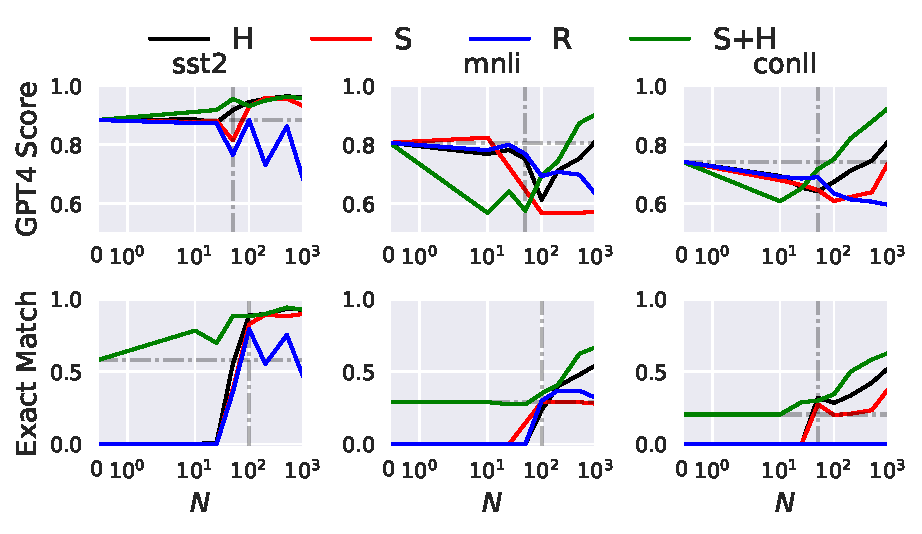
\includegraphics[width=0.8\textwidth]{images/learning_dynamics/sym_exp1.pdf}
    \caption[IFT training data mixes]{Incorporating  $0 \leq N \leq 1000$ (H)uman, (S)ynthetic and (R)andomly labeled synthetic data samples in IFT training set. (S+H) is trained on 100 synthetic samples, then $N$ human data samples. }\vspace{-.8cm}
    \label{fig:random}
\end{figure}



\subsection{$\mathcal{S}_2$: IFT models as Task-Specific Solvers}

%Motivated by industrial considerations, we delve into $\mathcal{S}_2$, which focuses on specializing IFT models on a specific task.

\noindent \textbf{Setting.} We use four model architectures and, for each architecture, we employ the base model to train an IFT model variant using the synthetic Alpaca dataset. We then fine-tune both the base models and their IFT variants on a subset of $N$ samples drawn from the target task. This setup simulates an industrial scenario in which limited data is available to specialize a model on a unique task, and assesses whether there are benefits to instruction-tuning a base model before fine-tuning it on the target task. 
\\\noindent \textbf{Results}. \autoref{fig:exp4} demonstrates that IFT models exhibit enhanced performance in low-data scenarios (when $10 \leq N \leq 200$). 
Intuitively, IFT models are better able to leverage the task description given in the prompts, thus enabling boosted zero-shot performance \sidecite{scao2021data}. This complements and steers model training when finetuned with small numbers of samples. When more samples are available ($N \geq 200$), the task pattern is sufficiently clear and the benefits of prompting and of the IFT training phase disappear.

 
\begin{figure}[ht]
    \centering
    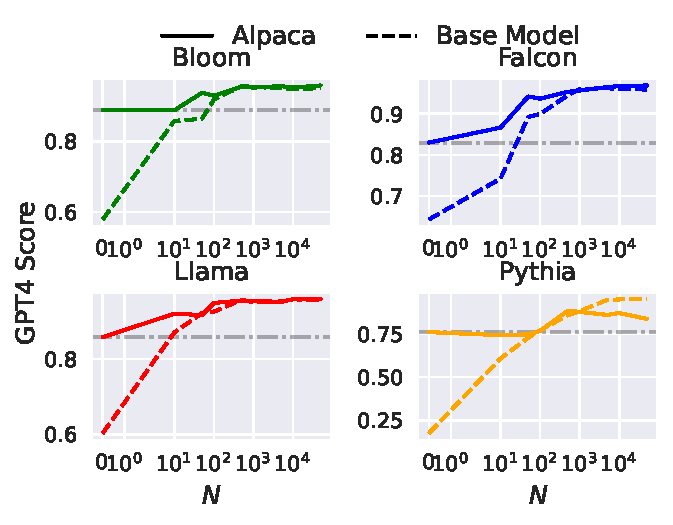
\includegraphics[width=0.8\textwidth]{images/learning_dynamics/exp4_all.pdf}
    \caption[GPT4 SST-2 scores]{GPT4 score on SST-2 test set after finetuning with $0 \leq N \leq 1000$  samples on a (base) LM or an IFT model. Further experiments can be found in \autoref{sec:extra-datasets-exp4}. }
    \label{fig:exp4}
\end{figure}

This finding aligns with the results presented in \autoref{ssec:scenario1}, emphasizing the potential of synthetic datasets to enhance data efficiency in industrial scenarios.


\section{Key Takeaways for Practitioners}
\label{sec:conclusion}

\noindent \textbf{Leveraging LLM for evaluation.} Evaluating IFT models is challenging, as it mandates \emph{comparability across tasks} and \emph{format-agnostism}, which standard metrics struggle with. While LLM scoring is not ideal (Limitations in \autoref{sec:limitations}), it is a strong option practitioners should add to their arsenal.
%consider in their evaluation strategy.
\\\noindent \textbf{Leveraging Synthetic Data for Efficient Learning.} LLM-based evaluation uncovers the fact that leveraging synthetic data provides a quick and cost-effective approach to mastering format in low data regimes, with no performance degradation. This methodology proves viable across various scenarios, presenting an opportunity to more efficiently leverage potentially limited amounts of expert annotated data available.
% significantly lower costs, which is particularly advantageous when incorporating expert annotations.



%Intuitively, including the target task in an IFT training set leads to better performance. However, performance improvements on a given task are only truly seen once the format is learned. Until then, performance tends to stay stable, or even decrease.
%\\\noindent Using an IFT model as the base model for fine-tuning offers large performance gains in very low shot training settings. Passed a certain number of shots, this benefit fully disappears.


% \section{Conclusion}
% 1 on highlight les limitations, le pb c'est qu'il n'y a que GPT4 (discusssed in limitation)
% 2 provide take-home lessons for practitionner and



%\input{conclusion.tex}

% \subsection{Citations}

% We encourage you to use the natbib styles.
% You can use the command \verb|\sidecite| (cite in text) to get ``author (year)'' citations, like this citation to a paper by \sidecite{layoutlm}.
% You can use the command \verb|\sidecite| (cite in parentheses) to get ``(author, year)'' citations \sidecite{layoutlm}.
% You can use the command \verb|\citealp| (alternative cite without parentheses) to get ``author, year'' citations, which is useful for using citations within parentheses (e.g. \citealp{layoutlm}).

\section*{Limitations}
\label{sec:limitations}
While this paper has argued in favor of using LLM as scorers, important drawbacks remain. 
The best-performing scorer at the moment, GPT4 is a proprietary, black-box access model, and no guarantees exist that it will remain accessible unchanged over time, leading to reproducibility issues and data privacy concerns. Since model and training data internals are not open-knowledge, analysis of scoring errors and internal model biases is also limited. 

Promising openly available alternative models are being developed, either general purpose LLMs aiming to disrupt the hegemony of GPT4 \cite{touvron2023llama2, bai2023qwen}, or smaller models specialized for automatic evaluation, often attempting to distillate GPT4's scoring abilities by training on GPT4 generated scores or scoring explanations \sidecite{xu2023instructscore, liu2023geval}. In the latter category, the Prometheus scoring model \sidecite{kim2023prometheus}, based on Llama2, claims scoring performances on par with GPT4 in terms of human score correlations over a variety of tasks and benchmarks. Eventually, strong Open-Source LLMs should alleviate most of the concerns raised by relying on proprietary black-box models and we hope this work, by shedding light on the importance of LLM scoring, motivates these efforts to build open models with strong scoring abilities. 
% Pertaining to reproducibility, LLM scorers are sensitive to scoring prompt formulations. While not a problem in practice since the same prompt can be used across evaluations, some prompts are bound to be better than others, which will necessarily lead to various prompts being used across the literature, and hindering researcher ability to compare results against externally claimed baselines. 


% As seen in our experiments, to unlock truly good scoring, it is necessary for the scoring model to outperform evaluated models on the given task. While a large limitation of this scoring paradigm, weaker models can still evaluate better models on criteria they manage well, such as text coherence, relevance to the prompt, grammar, etc. even if the underlying task comprehension is not on-par. Work like INSTRUCTScore also show promising results of distilling GPT4 evaluation skills in smaller models like LLaMA 7B for specific tasks like translation.
% 


% ACL 2023 requires all submissions to have a section titled ``Limitations'', for discussing the limitations of the paper as a complement to the discussion of strengths in the main text. This section should occur after the conclusion, but before the references. It will not count towards the page limit. The discussion of limitations is mandatory. Papers without a limitation section will be desk-rejected without review.

% While we are open to different types of limitations, just mentioning that a set of results have been shown for English only probably does not reflect what we expect. Mentioning that the method works mostly for languages with limited morphology, like English, is a much better alternative. In addition, limitations such as low scalability to long text, the requirement of large GPU resources, or other things that inspire crucial further investigation are welcome.

\section*{Ethics Statement}
% Scientific work published at ACL 2023 must comply with the ACL Ethics Policy.\sidenote{\url{https://www.aclweb.org/portal/content/acl-code-ethics}} We encourage all authors to include an explicit ethics statement on the broader impact of the work, or other ethical considerations after the conclusion but before the references. The ethics statement will not count toward the page limit (8 pages for long, 4 pages for short papers).

While this work intends to evaluate scorers across many different tasks and settings, it is essentially English-centric, and no conclusions are drawn about the robustness of LLM scorers in other languages. LLM scoring may also be affected by internal model bias acquired through pretraining or subsequent finetuning, and while efforts are made by OpenAI to mitigate bias, critical applications of LLM evaluation should consider that truly objective evaluation is not attainable.

All data and base models used in this work originate from publicly available sources. The GPT4 Alpaca dataset is a variant of \sidecite{alpaca2023} built from synthetic data only, collected through the OpenAI API. The non-synthetic data are sourced from manually annotated, widely used datasets for NLP benchmarking. This work does not transgress any usage restrictions associated with these data sources. Base models used are either available through fully open-source licenses (Falcon, Pythia), or licenses with no restrictions for research purposes (LLaMA, Bloom). 

We estimate our experiments consumed 5500 GPU V100 hours, using a low-carbon compute cluster, amounting to about 950 kg of CO2 over the course of the project.  To reduce the impact to a maximum, all runs are done through the efficient Low-Rank Adaptation training strategy \sidecite{hu2021loralowrankadaptationlarge}, and only trained adapter weights are stored to minimize bandwidth and memory usage. API calls to external APIs are cached to minimize redundancies.


\section*{Acknowledgements}
This work is partially supported by Illuin Technology, and by a grant from ANRT France.
This work was performed using HPC resources from GENCI–IDRIS (Grant 2023-AD011014185).
Secondary compute contributions were made on HPC resources (Grant 2023-AD103256) and (Grant 2023-AD101838).

% \chapter{ColPali Appendix}

\section*{Reproducibility Statement}

For transparency, reproducibility and to foster future work, we release our training data, model checkpoints (adapters), entire codebase, and complete evaluation benchmark under MIT licenses as detailed in the main paper. We also host a public \textsc{ViDoRe} leaderboard\sidenote{\url{https://huggingface.co/spaces/vidore/vidore-leaderboard}} to foster concurrent work in the space. The supplementary material further details training configurations for our models (also specified in HuggingFace model repositories), and dives into the process we used to generate synthetic data, how latency computations are performed, as well as provides further detailed evaluation results.



\section*{Acknowledgements}

This work is partially supported by Illuin Technology, and by a grant from ANRT France. This work was performed using HPC resources from the CINES ADASTRA through Grant 2024-AD011015443 and from IDRIS with grant 2024-AD011015724R1.
We extend our warm thanks to Jonathan Dong, Caio Corro, Victor Pellegrain and Ender Konukoglu for their valuable feedback on the paper.


\section{Benchmark Datasets}

\subsection{Academic Datasets}
\label{subsection:academic_datasets}

\noindent\textbf{DocVQA} \sidecite{mathew_docvqa_2020} includes collected images from the UCSF Industry Documents Library. Questions and answers were manually annotated.

\noindent\textbf{InfoVQA} \sidecite{mathew_infographicvqa_2021} includes infographics collected from the Internet using the search query “\textit{infographics}”. Questions and answers were manually annotated.

\noindent\textbf{TAT-DQA} \sidecite{zhu_towards_2022} is a large-scale Document VQA dataset that was constructed from publicly available real-world financial reports. It focuses on rich tabular and textual content requiring numerical reasoning. Questions and answers were manually annotated by human experts in finance.

\noindent\textbf{arXivQA} \sidecite{li2024multimodal} is a VQA dataset based on figures extracted from arXiv publications. The questions were generated synthetically using GPT-4 Vision.

\noindent\textbf{TabFQuAD} (Table French Question Answering Dataset) is designed to evaluate TableQA models in realistic industry settings. We create additional queries to augment the existing human-annotated ones using the same method described in \autoref{subsection:docvisbench_methodology}.

\label{subsection:tabfquad}
% create new queries following the same methodology as in\autoref{paragraph:query_generation} but with GPT-4 Vision. Eventually, we obtained a retrieval version of TabFQuAD with 1,800 document query pairs, which we split into a training set of 1550 examples and a test set of 250 examples.


\subsection{Practical Datasets}
\label{subsection:docvisbench_methodology}
%Hugging Face collection: \url{https://huggingface.co/collections/coldoc/syntheticdocqa-test-6655c59cfda461267c0d9ac8}

% \subsubsection{Method}

\noindent\textbf{Methodology.} Creating a relevant retrieval dataset close to real use cases is a major challenge as the dataset needs to be both sufficiently large for effective fine-tuning and sufficiently diverse to cover a broad range of modalities (full text, tables, charts, ...), domains (industry, healthcare, ...), and query-document interactions (extractive questions, open-ended questions, ...). Our approach to building this dataset involves several steps: (1) we use a web crawler to collect publicly available documents on various themes and sources, (2) we convert these PDFs into a series of images, one per page, and (3) we generate queries related to each image using a VLM.

\noindent\textbf{Web-Crawler.} We implemented a web crawler to efficiently collect large volumes of documents related to a given topic. The crawler is seeded with a user-defined query (e.g.\ ``artificial intelligence") and then uses GPT-3.5 Turbo to brainstorm related topics and subtopics. This query augmentation strategy aims at both broadening and deepening the search. GPT-3.5 Turbo is further used to generate diverse search queries from each subtopic. This query set is then consumed by a pool of parallel workers whose job is to fetch the associated most relevant documents. We use SerpAPI\sidenote{\url{https://serpapi.com/}} along with a filetype filter (PDF documents only) to programmatically scrape Google Search rankings. Each file is hashed and stored in a Bloom filter \sidecite{bloom_spacetime_1970} shared among workers to avoid duplicate documents in the final corpus. Unique scraped files are downloaded, and inserted into a SQLite database along with additional metadata.

\noindent\textbf{Datamix.} Using the web crawler, we collected approximately 100 documents for each of the following four seeds: \textit{``energy"}, \textit{``government reports"}, \textit{``healthcare industry"}, and \textit{``artificial intelligence"}. These seeds were meticulously hand-picked to align with real-use cases for retrieval models and visually rich pages. We also removed all documents containing any private information. 

\noindent\textbf{Query Generation.}\label{paragraph:query_generation} To increase the efficiency of our query generation scheme and to limit API calls, we generate at most 3 questions per image. From all the documents collected, we randomly sample 10,000 images per theme and call Claude-3 Sonnet with the following prompt:


\begin{kaobox}

You are an assistant specialized in Multimodal RAG tasks.

The task is the following: given an image from a pdf page, you will have to 
generate questions that can be asked by a user to retrieve information from 
a large documentary corpus. 
The question should be relevant to the page, and should not be too specific 
or too general. The question should be about the subject of the page, and 
the answer needs to be found in the page.

Remember that the question is asked by a user to get some information from a
large documentary corpus that contains multimodal data. Generate a question 
that could be asked by a user without knowing the existence and the content 
of the corpus.
Generate as well the answer to the question, which should be found in the
page. And the format of the answer should be a list of words answering the
question.
Generate at most THREE pairs of questions and answers per page in a dictionary
with the following format, answer ONLY this dictionary NOTHING ELSE:

{
    "questions": [
        {
            "question": "XXXXXX",
            "answer": ["YYYYYY"]
        },
        {
            "question": "XXXXXX",
            "answer": ["YYYYYY"]
        },
        {
            "question": "XXXXXX",
            "answer": ["YYYYYY"]
        },
    ]
}
where XXXXXX is the question and ['YYYYYY'] is the corresponding list of answers
that could be as long as needed.

Note: If there are no questions to ask about the page, return an empty list.
Focus on making relevant questions concerning the page.
Here is the page:

\end{kaobox}

% \subsection{TabFQuAD}
% \label{subsection:tabfquad}
% \noindent\textbf{Data Collection.} TabFQuAD (Table French Question Answering Dataset) is designed to evaluate TableQA models in realistic industry settings. TabFQuAD is created by: (1) using an internet scrapper to retrieve PDF documents from the websites of large companies and government agencies (2) using a custom table extraction pipeline based on both manual heuristics and deep learning methods to detect \sidecite{huang_layoutlmv3_2022} and reconstruct \sidecite{qiao_lgpma_2021} tables from the original PDF documents, and (3) manually inspecting each table and filter out low-quality extractions. In the end, we obtain 2,308 industry-realistic tables from a wide range of sources. While this process was designed to automate a large part of the work, we believe having a human evaluation step was required to ensure high-quality data that does not propagate errors from the extraction pipeline.

% \begin{figure}
%     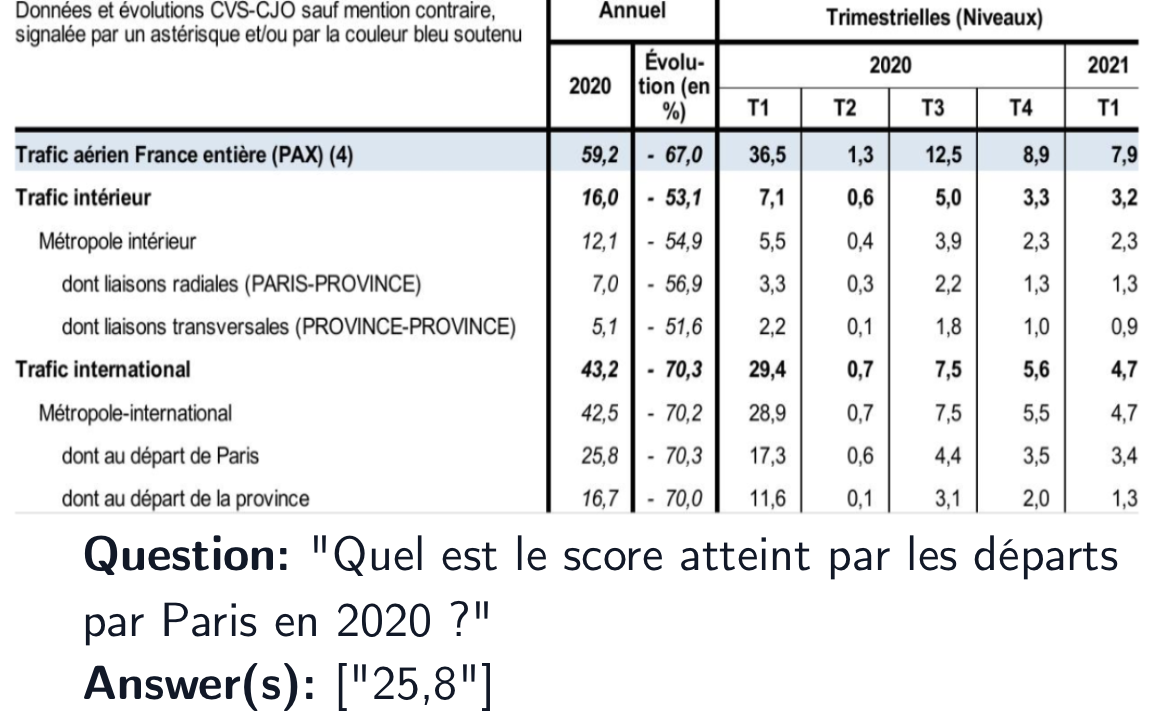
\includegraphics[width=0.45\textwidth]{images/colpali_images/dataset_samples/tabfquad_example.png}
%     \caption{TabFQuAD contains visually rich tables, e.g. this example with highlighted numbers, cell background, and custom cell lines for delimiting subcategories.}
% \end{figure}

% \noindent\textbf{Integration in \textit{ViDoRe}.}
% For our use case, we used the test set of TabFQuAD by filtering out adversarial questions as we are interested in a retrieval task.
% In the original TabFQuAD dataset, we observed that certain questions are irrelevant to the retrieval task. For instance, \textit{When was the project created?} (in French, \textit{Quand a été crée le projet ?}) is too vague. Thus, we have decided to keep the table images but to create new queries following the same methodology as in\autoref{paragraph:query_generation} but with GPT-4 Vision. Eventually, we obtained a retrieval version of TabFQuAD with 1,800 document query pairs, which we split into a training set of 1550 examples and a test set of 250 examples.

\noindent\textbf{Human Validation.} We manually validate every single synthetically created query in \textsc{ViDoRe} to ensure quality, query relevance, and consistency with the benchmark objective of evaluating retrieval in practical industrial settings. During this step, we randomly assign document-pair queries to 4 volunteer annotators and instruct them to filter out queries that do not fit the above-listed criteria. We also instruct annotators to flag any documents they deem to contain PII information or content not suited for an academic benchmark. No flag was raised during the entirety of the process, validating our prior PDF collection strategy. 100 queries per topic are collected in this manner. Annotators are colleagues and collaborators of the authors who volunteered to help. Each annotator spent approximately 3 hours filtering the larger query set down to 100 high-quality queries per topic.

\subsection{Training Dataset}
\label{subsection:training_dataset}
The statistics of the train set are given in the following table. The creation of the train set follows the same methodology as in \autoref{subsection:docvisbench_methodology}. We made sure that a PDF document cannot have pages in both the training set and the test set to prevent data leakage and that there are no duplicate documents in each split.

\begin{table}[ht]
    \centering
    \label{tab:datasets}
    \small
    \begin{tabular}{llll}
        \toprule
        \textbf{Dataset Split} & \textbf{Split Size} & \textbf{Language} & \textbf{Domain}\\
        \midrule
        DocVQA & 39,463 & English & Scanned documents from UCSF Industry\\
        InfoVQA & 10,074 & English & Infographics scraped from the web \\
        TATDQA & 13,251 & English & High-quality financial reports \\
        arXivQA & 10,000 & English & Scientific Scientific Figures from arXiv\\
        Scraped PDFs & 45,940 & English & Varied PDFs from 3885 distinct URL domains\\
        \midrule
        \textbf{TOTAL} & \textbf{118,695} & \textbf{English-only} & \textbf{Mixed} \\
        \bottomrule
    \end{tabular}
    \caption[ColPali dataset splits]{Details on the different splits in the dataset used to train ColPali.}
    \label{table:training_set_overview}
\end{table}
% \newpage



\section{Implementation details}

\subsection{Codebase}
The codebase is written in PyTorch\sidenote{\url{https://pytorch.org/}} and leverages HuggingFace tooling for model implementations and trainers\sidenote{\url{https://huggingface.co}}.


\subsection{Hyperparameters}

Hyperparameters are tuned on a validation split composed of $2\%$ of the training dataset. We find bi-encoder methods to be more sensible to learning rate variations than late interaction-based models and achieve the best performance for all models with a learning rate of $5e-5$. We experiment with LoRA rank and $\alpha$ values and do not notice particular improvements past $r = \alpha = 32$. Per-device batch sizes are kept small due to long sequence lengths that complicate scaling past $b=4$. We simulate larger batch sizes with multi-GPU training and train with a total batch size $b=32$ with no accumulation, for 1 epoch on our training set.


\subsection{Embedding size}
\label{subsection:embedding_size}

Minimizing storage footprint can be essential to industrial retrieval systems if databases contain millions of documents. With this criterion in view, we have compared the embedding sizes of the models in our study. As shown in \autoref{table:embedding_size}, \textit{ColPali}’s embedding size is an order of magnitude larger than BM25 and two orders of magnitude larger than BGE-M3. However, in practical scenarios, pooling multi-vector embeddings by centroid cluster, or quantizing embeddings to binary representations \sidenote{\url{https://blog.vespa.ai/scaling-colpali-to-billions/}} can reduce storage costs by two orders of magnitude \sidecite{santhanam_plaid_2022} with minimal performance hits, and make storage costs competitive with other systems.

\begin{table}[ht]
    \centering
    \begin{tabular}{l|c}
    % \hline
    \textbf{Model}              & \textbf{Embedding size (KB)} \\
    \hline
    BGE-M3             & 8.60               \\
    BM25 (dense emb.)  & 3.00                \\
    BM25 (sparse emb.) & 1.56 ± 0.51         \\
    \textit{ColPali} (float16)            & 257.5              \\
    % \hline
    \end{tabular}
    \caption[DocVQA embedding sizes]{Comparison of the embedding sizes for the DocVQA test set from \textsc{ViDoRe} w.r.t. different retrieval models. The \textit{mean ± std} size is given for the sparse embeddings. In general multiple vectors (2-5) per page are used for BGE-M3 and BM25.}
    \label{table:embedding_size}
\end{table}


\subsection{Latency computations}
\label{paragraph:latency_app} 
To ensure comparison fairness, the latencies of the different retrieval systems shown in \autoref{fig:latency-comparison} are measured on the same \texttt{g2-standard-8} GCP VM with an NVIDIA L4 GPU. Document pages are embedded using the highest settings of \texttt{Unstructured} with captioning (see \autoref{subsection:baseline_models}). SigLIP and \textit{ColPali} are both loaded with \texttt{bfloat16} parameter dtypes. The reported times in \autoref{table:latency-comparison} are the average per-page latencies for each indexing operation on 1000 randomly chosen documents across all splits of the \textsc{ViDoRe} benchmark test set. A batch size of $8$ was used for the BGE-M3 model used with \texttt{Unstructured}, and a batch size of $4$ was used for SigLIP and \textit{ColPali}.

\begin{table}[ht]
    \centering
    \begin{tabular}{l|c|c|c}
    \multirow{2}{*}{\textbf{Indexing operation}} & \multicolumn{3}{c}{\textbf{Latency (s)}}                                                                      \\ \cline{2-4} 
                                                 & \multicolumn{1}{l|}{\textbf{Unstructured}} & \multicolumn{1}{l|}{\textbf{SigLIP}} & \textit{\textbf{ColPali}} \\
    \hline
    Layout detection                             & \multicolumn{1}{c|}{0.81}                  & \multicolumn{1}{c|}{NA}              & NA                                            \\
    OCR                                          & \multicolumn{1}{c|}{2.67}                  & \multicolumn{1}{c|}{NA}              & NA                                            \\
    Captioning                                   & \multicolumn{1}{c|}{3.71}                  & \multicolumn{1}{c|}{NA}              & NA                                            \\
    Page encoding                                & \multicolumn{1}{c|}{0.03}                  & \multicolumn{1}{c|}{0.12}            & 0.39                                          \\ \hline
    Total                                        & \multicolumn{1}{c|}{7.22}                  & \multicolumn{1}{c|}{0.12}            & 0.39
    \end{tabular}
    \caption[Page-level indexing latencies]{Page-level latencies for document indexing using various retrieval systems. SigLIP and \textit{ColPali} are much faster than \texttt{Unstructured} because they don't require the layout detection, OCR, and captioning operations.}
    \label{table:latency-comparison}
\end{table}


\subsection{Captioning}
\label{paragraph:captioning} 

Examples of captions generated for visually rich document chunks with Claude-3 Sonnet are shown in \autoref{fig:caption_table} and \autoref{fig:caption_figure}. The prompt used for generating the description is the following:

\begin{kaobox}
\small
You are an assistant specialized in document analysis. Given a table or a figure, you have to provide a detailed summary of the content in maximum 3000 characters. Your summary should be qualitative and not quantitative. Here is the table/figure to analyze: \{image\}. Answer ONLY with the caption of the table/figure.
\end{kaobox}

\begin{figure}[ht]
    \centering
    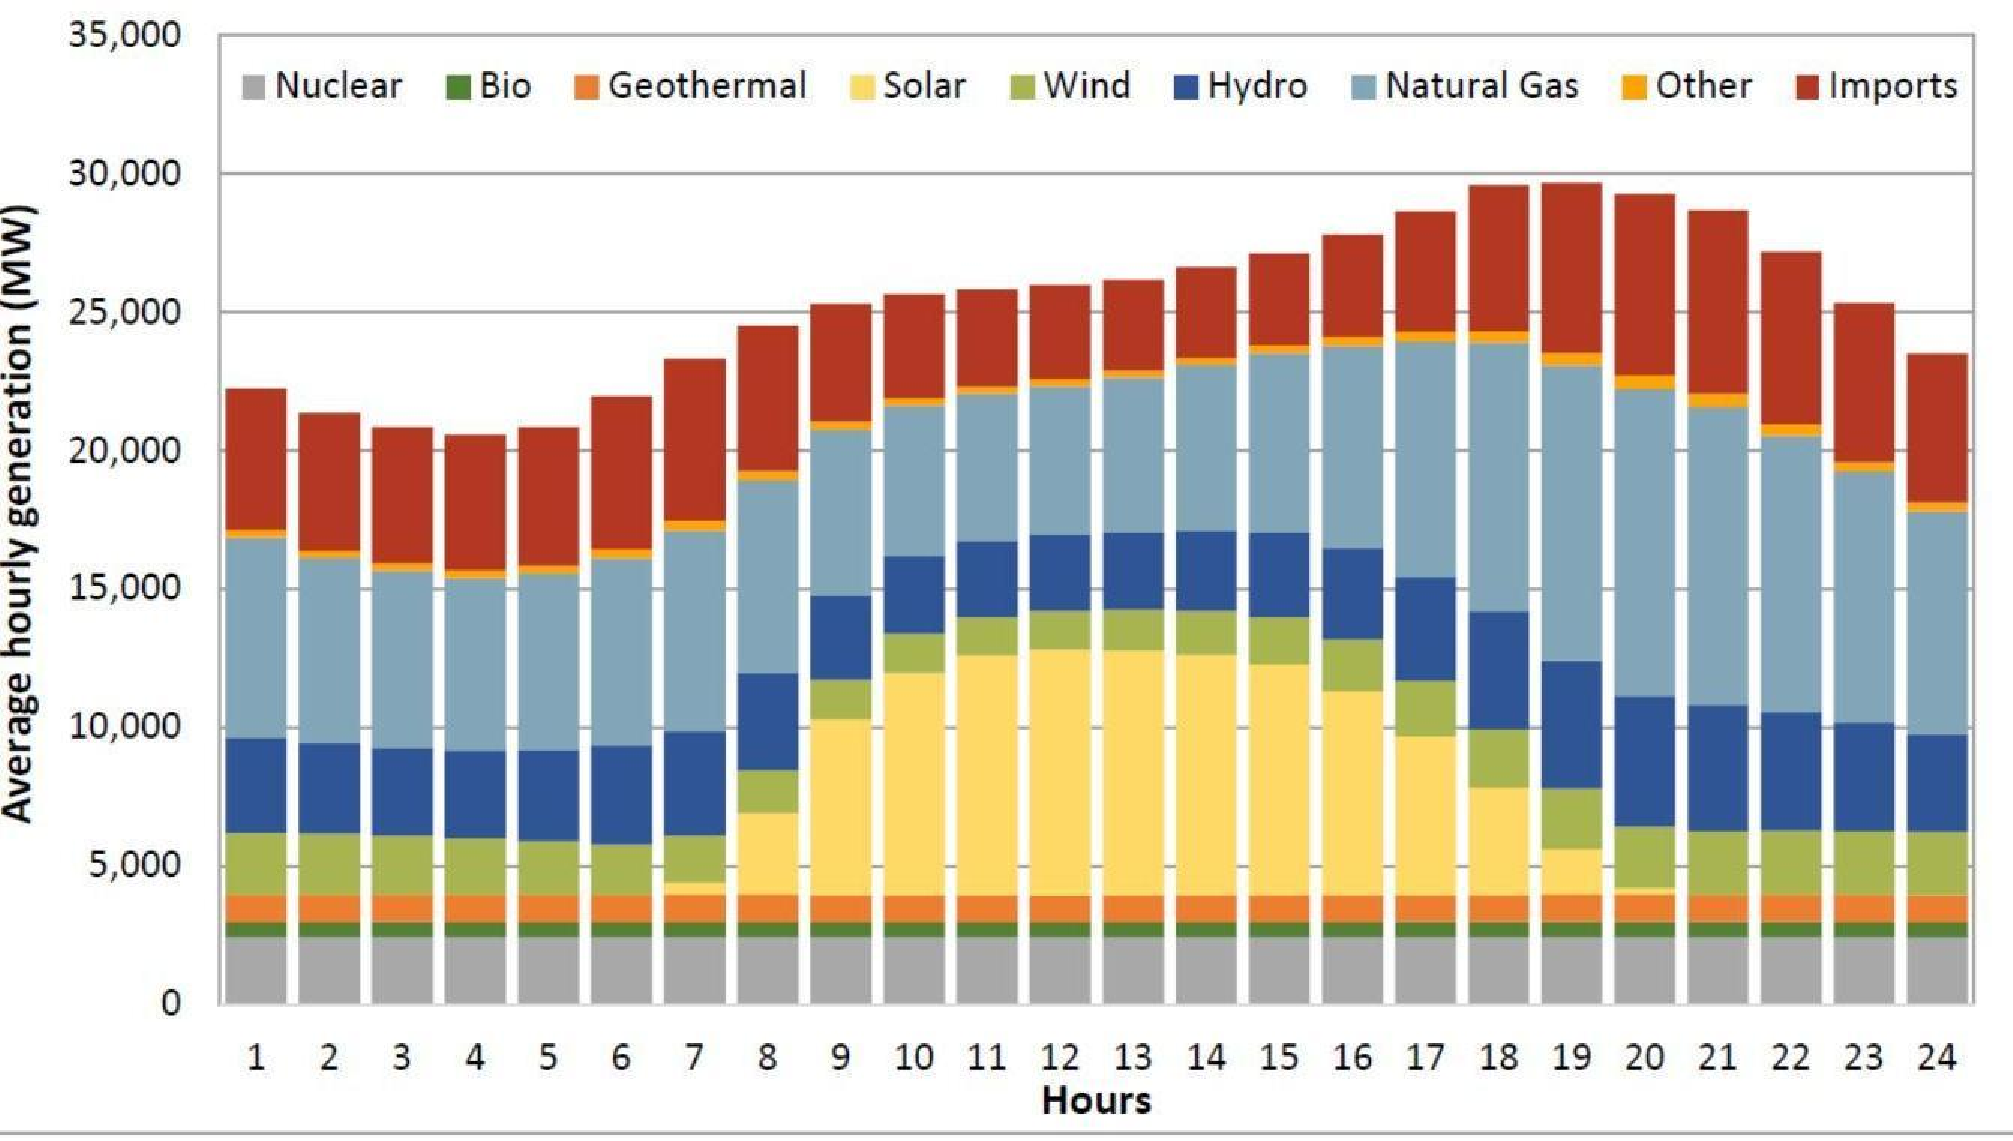
\includegraphics[width = 0.7 \textwidth]{images/colpali_images/ex_figure_caption.pdf}
    
    \caption[Energy test set example]{Example from the ``Energy" test set.\\
    \textbf{Caption:} \textit{The image depicts the hourly energy generation profile, illustrating the contributions of various energy sources over 24 hours. The data is presented as a stacked bar chart, with the x-axis representing the hours of the day from 1 to 2, and the y-axis showing the average hourly generation in MW. The bars are segmented into different colors, each representing a distinct energy source: nuclear, bio, geothermal, solar, wind, hydro, natural gas, and other imports. The chart provides insights into the temporal variations in energy generation across different sources, highlighting the interplay between baseload and intermittent sources throughout the day.}}
    \label{fig:caption_figure}
\end{figure}

% Table to do 

\begin{figure}[ht]
    \centering
    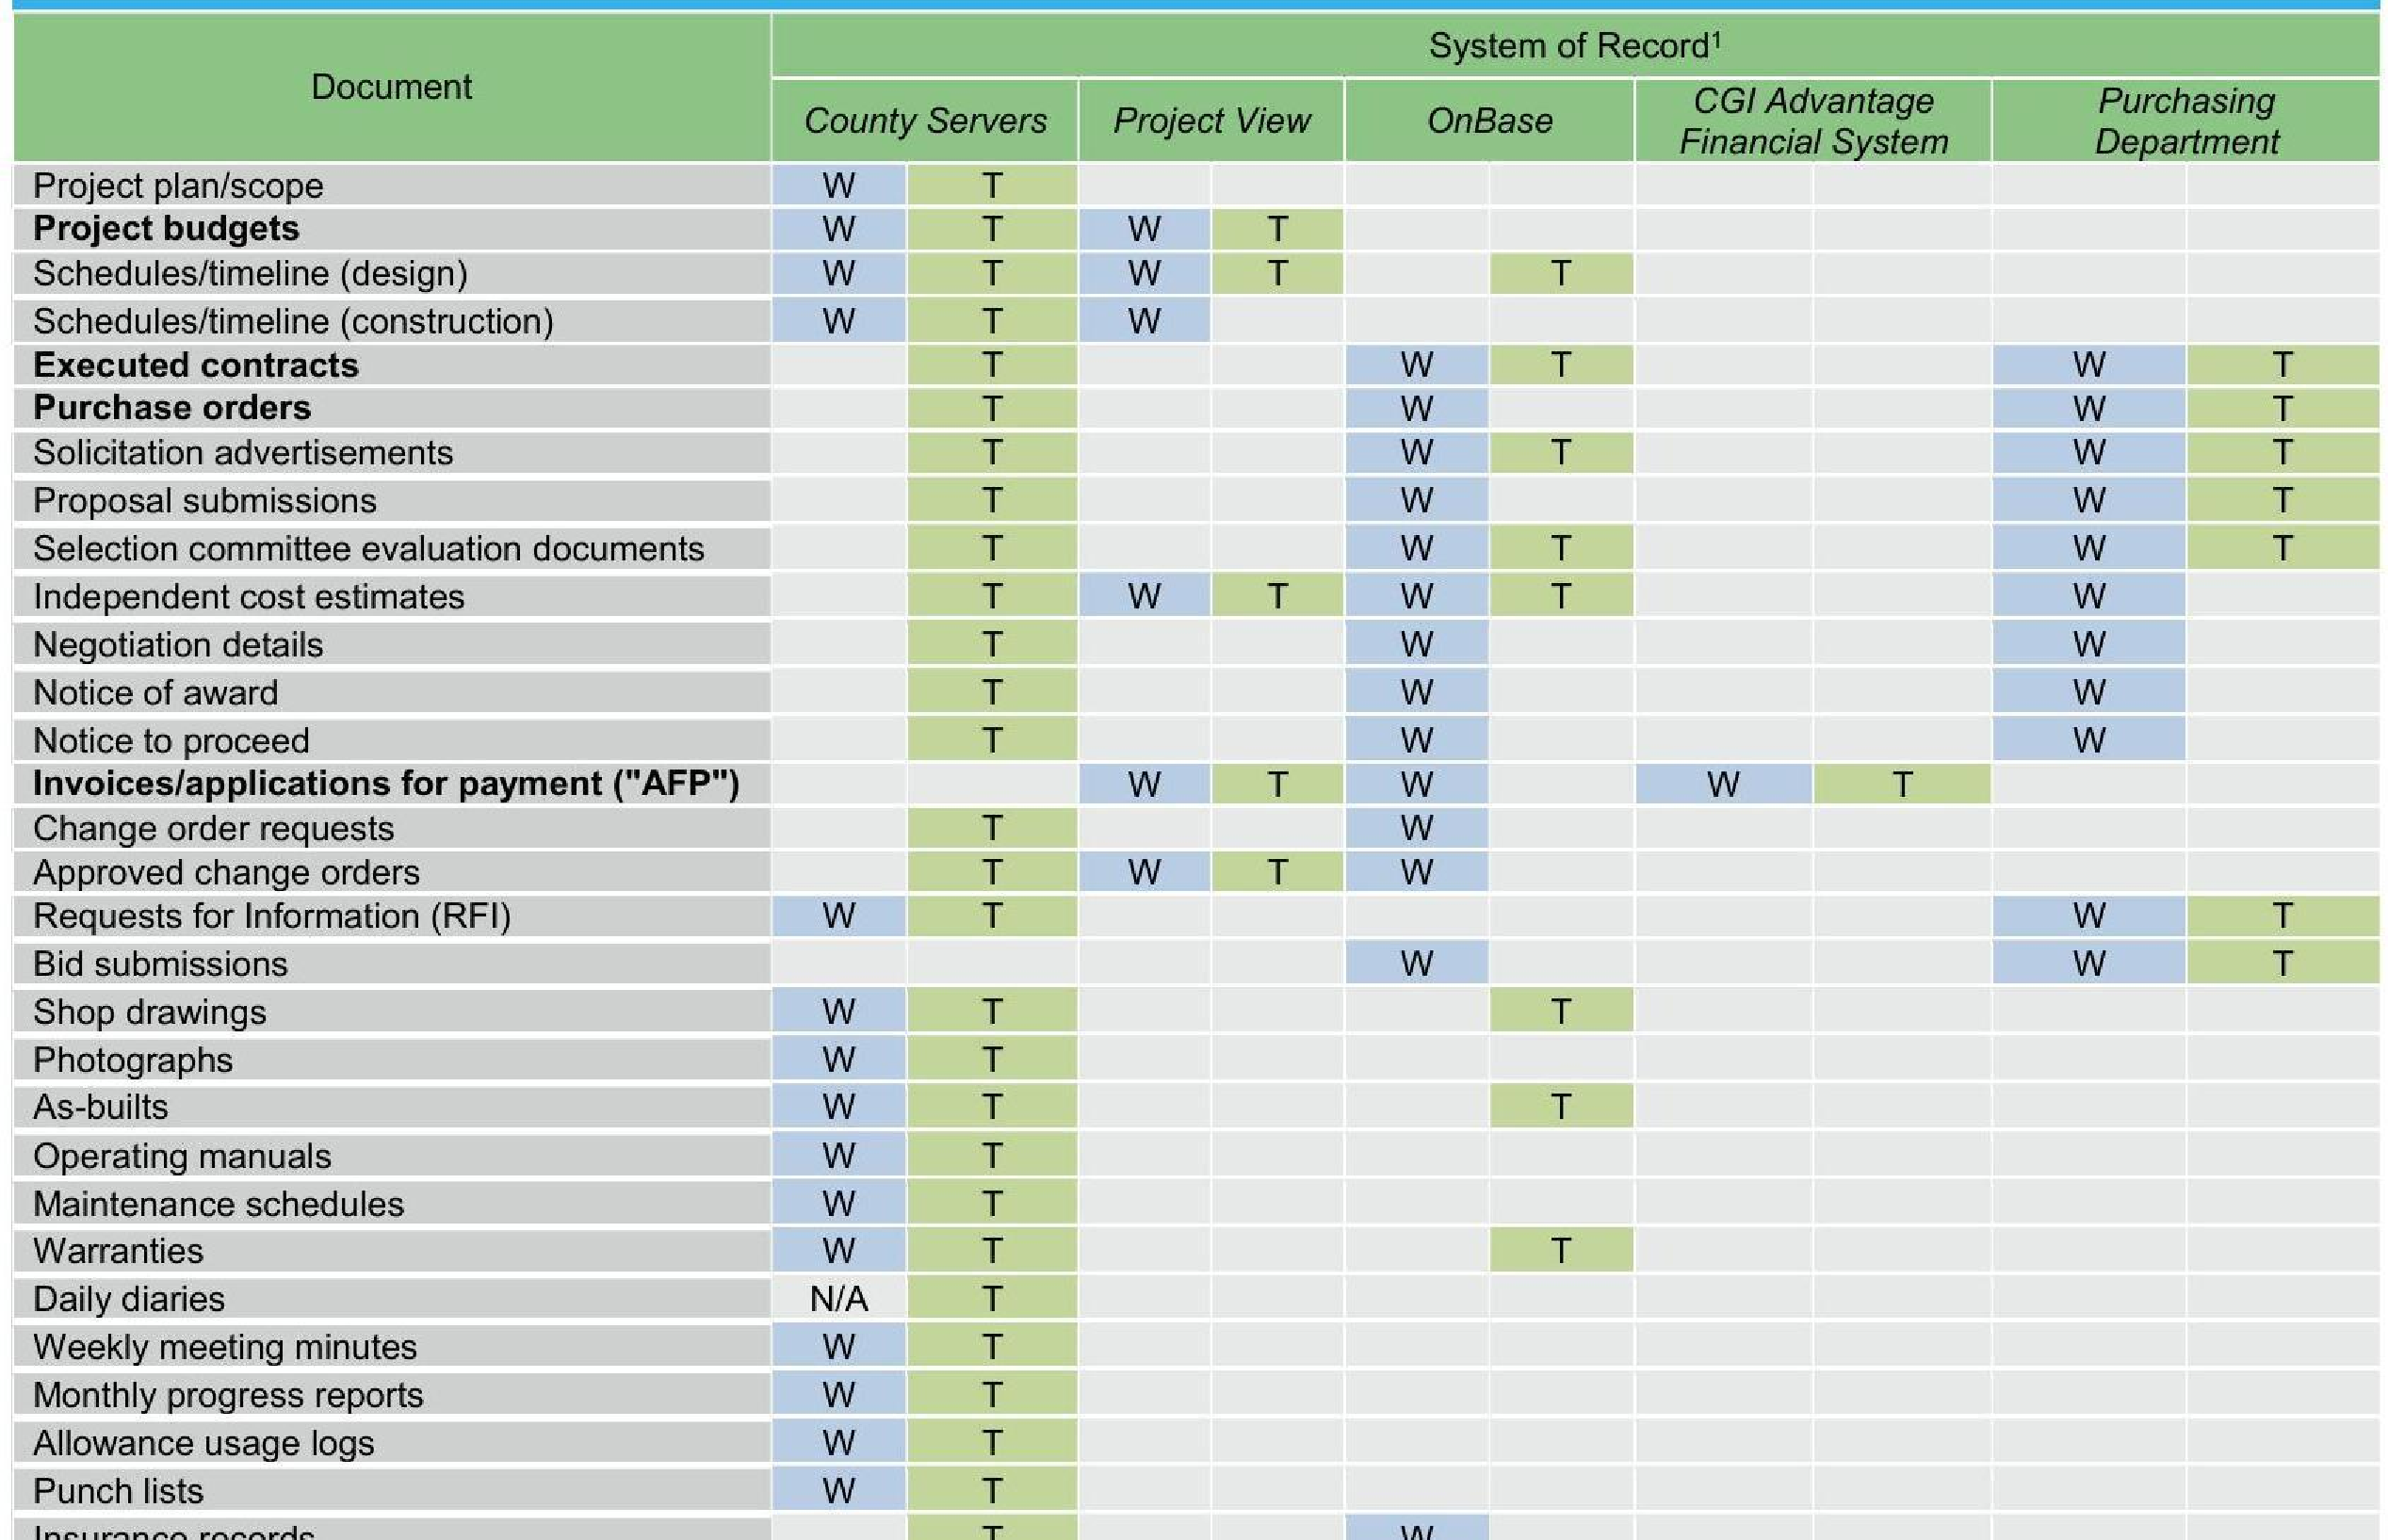
\includegraphics[width = 0.7 \textwidth]{images/colpali_images/ex_table_caption.pdf}
    
    \caption[Government reports example]{Example from the ``Government Reports" test set.\\
    \textbf{Caption:} \textit{The image shows a table titled ``System of Record" which outlines the different types of documents or records maintained across various systems or departments within an organization related to project management and construction. The rows list documents like project plans, budgets, schedules, contracts, purchase orders, invoices, change requests, bid submissions, drawings, manuals, meeting minutes, and reports. The columns indicate the system or department responsible for maintaining each record, such as County Servers, Project View, OnBase, CGI Advantage Financial System, and Purchasing Department. The table uses "W" and "T" markers to denote which system or department serves as the primary source (writer) or storage location (trailer) for each type of document.}}
    \label{fig:caption_table}
\end{figure}



% \newpage
% \section{More similarity maps}
% \label{section:more_similarity_maps}
% In \autoref{fig:similarity_map_kazakhstan}, \textit{ColPali} assigns a high similarity to all patches with the word \textit{"Kazakhstan"} when given the token \texttt{<\_Kazakhstan>}. Moreover, our model seems to exhibit world knowledge capabilities as the patch around the word \textit{"Kashagan"} - an offshore oil field in Kazakhstan - also shows a high similarity score. On the other hand, in \autoref{fig:similarity_map_ferroelectrics}, we observe that \textit{ColPali} is also capable of complex image understanding. Not only are the patches containing the word \textit{"formulations"} highly similar to the query token \texttt{\_formula}, but so is the upper-left molecule structure.

% \begin{figure}
% \centering
%     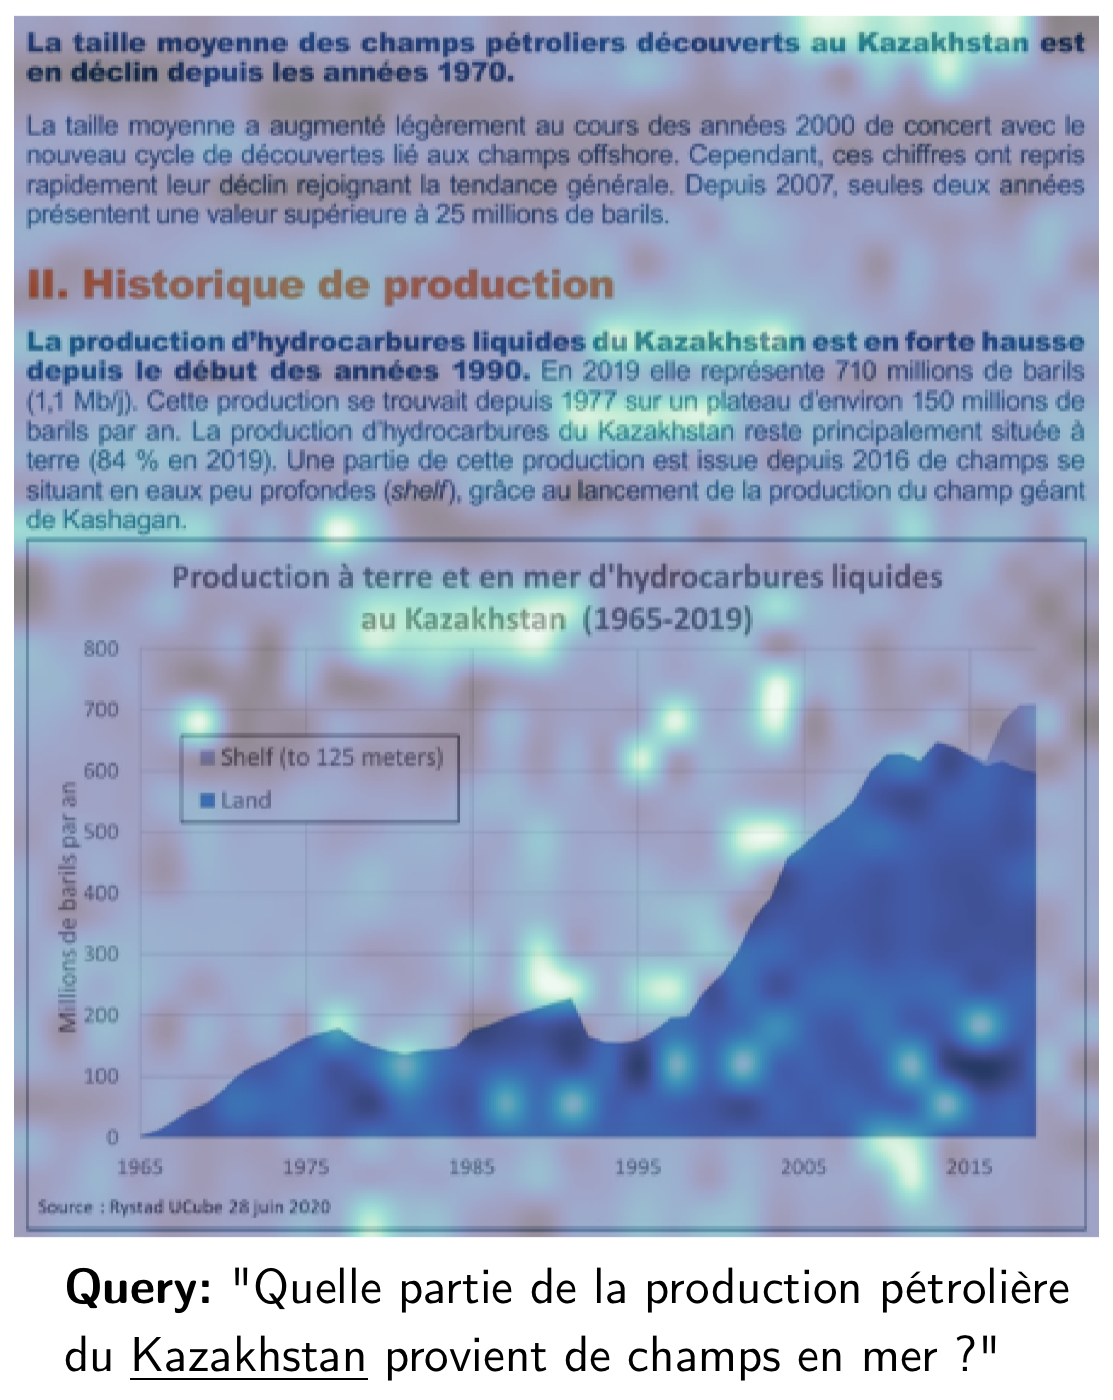
\includegraphics[width=0.8\linewidth]{images/colpali_images/similarity_maps/similarity_map_kazakhstan.png} 
%     \caption{Similarity of the image patches w.r.t. the underlined token in the user query. This example is from the \textit{Shift} test set.}
% \label{fig:similarity_map_kazakhstan}
% \end{figure}

% \begin{figure}
% \centering
% 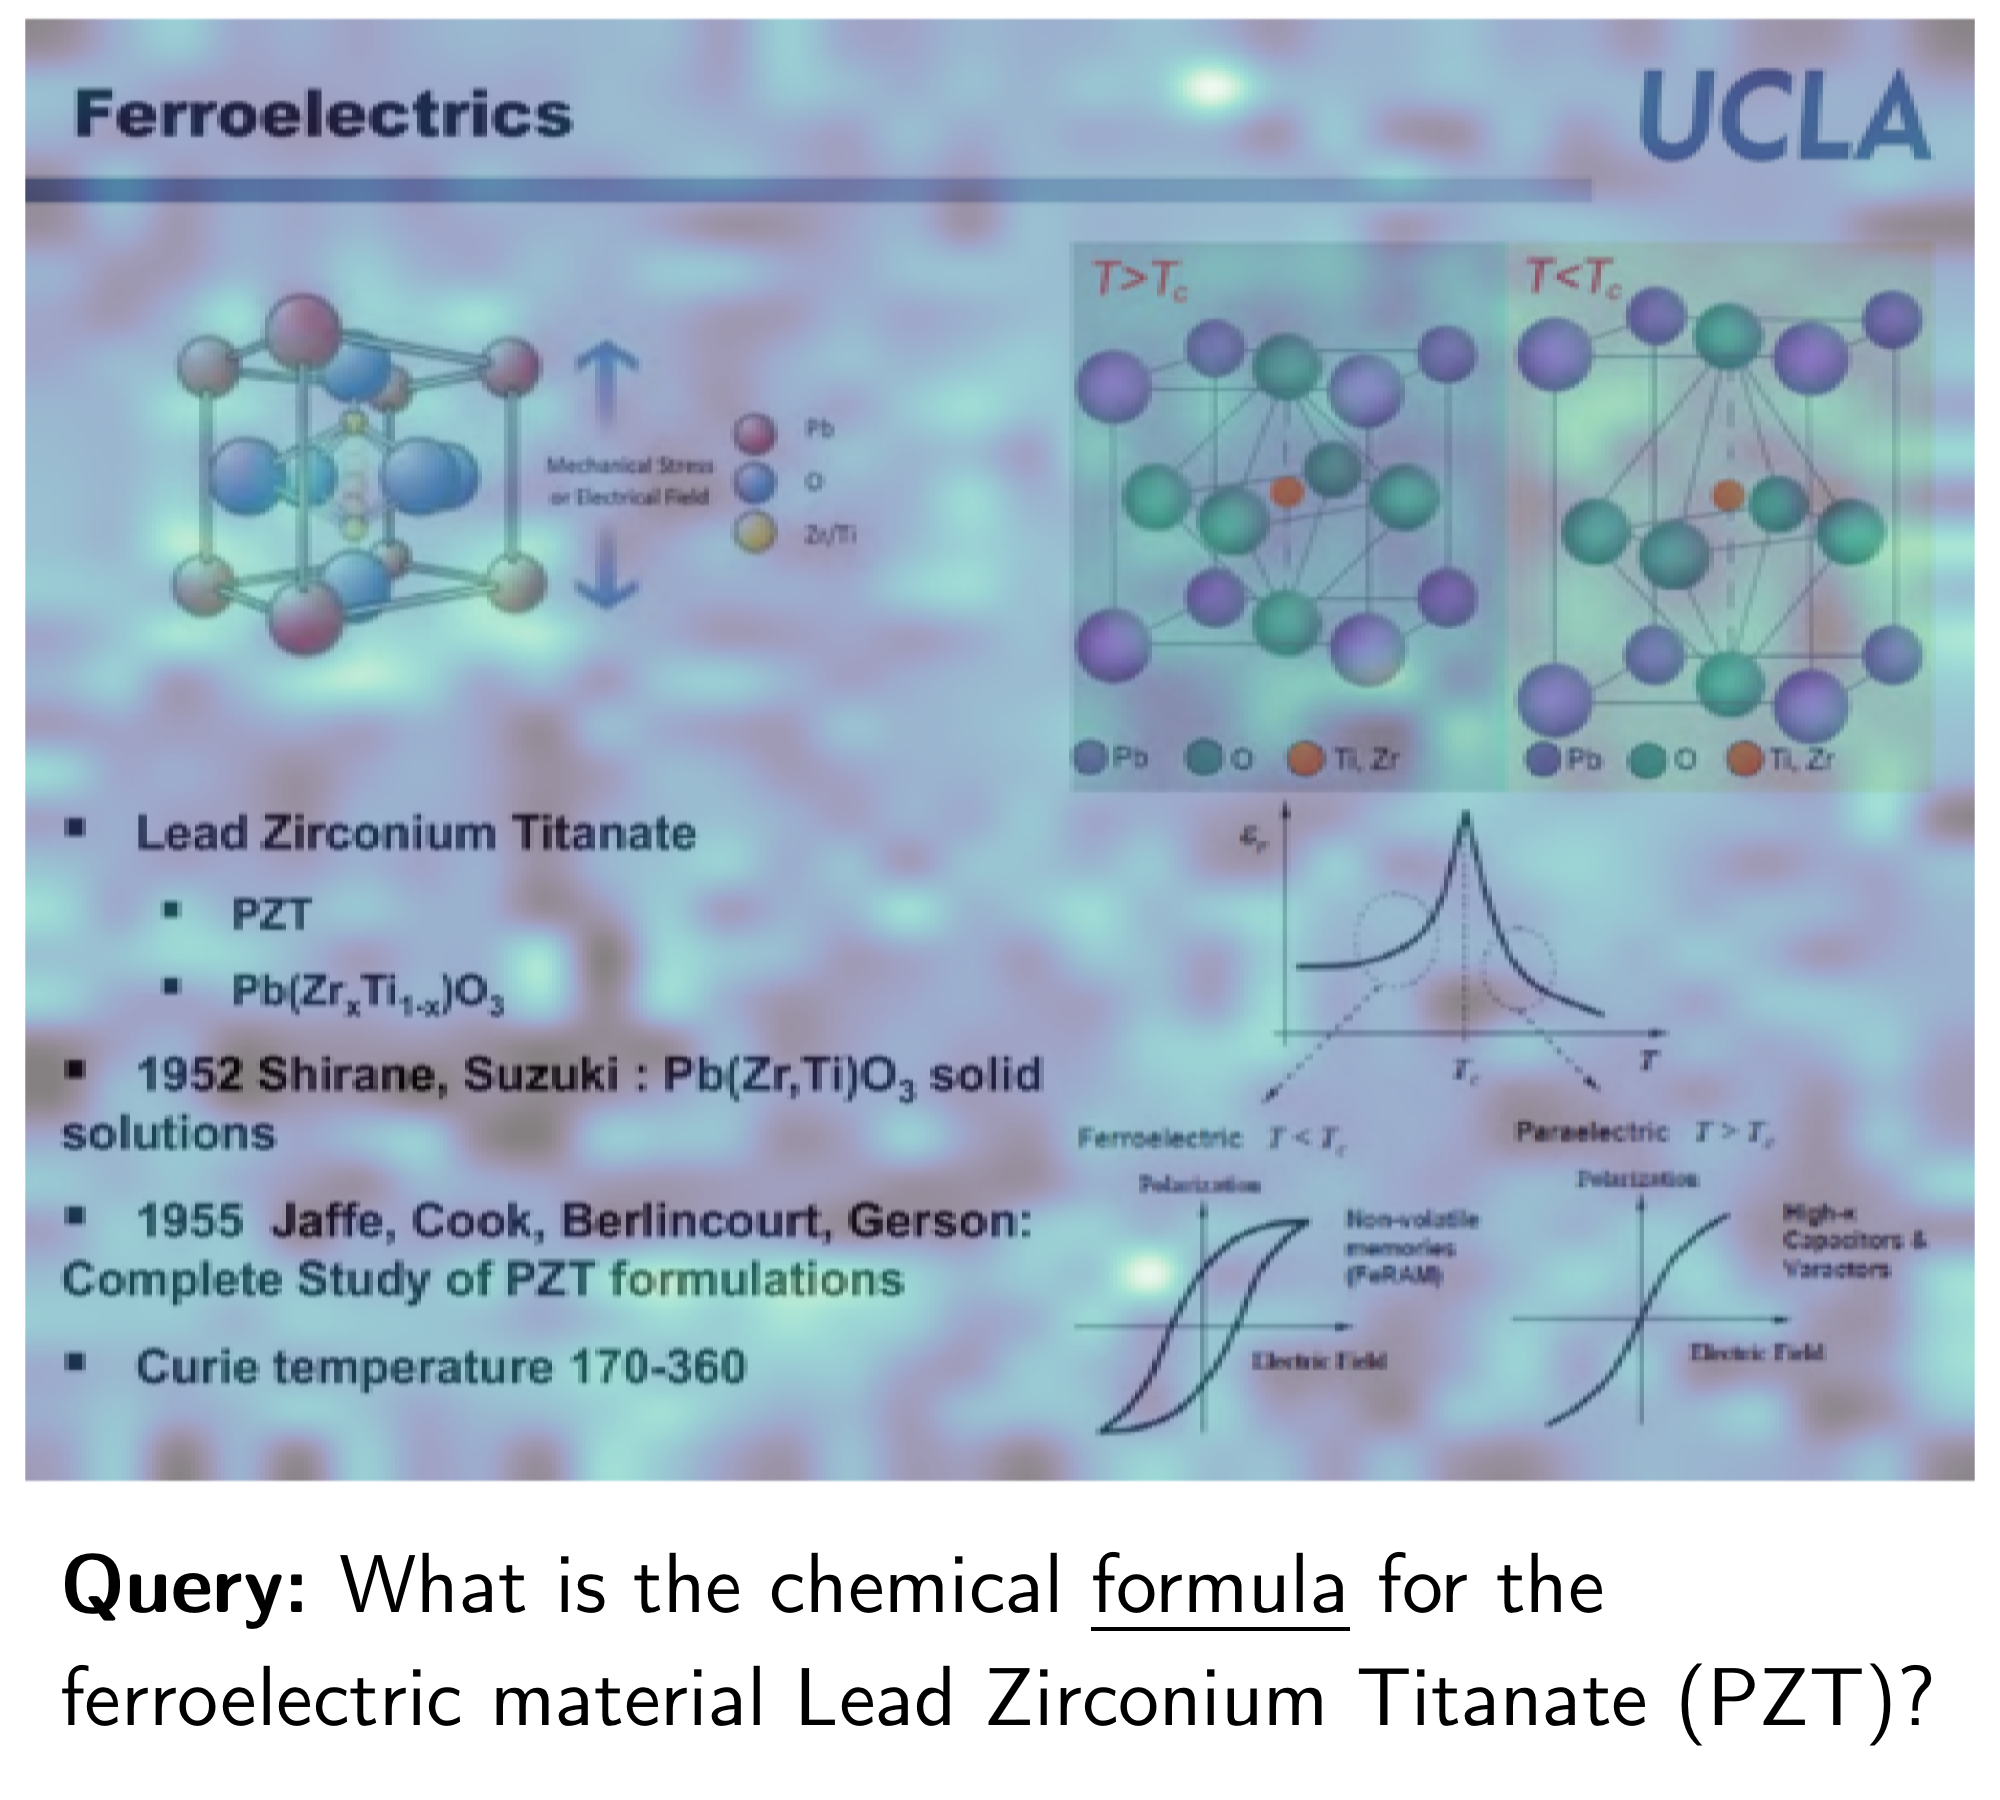
\includegraphics[width=0.95\linewidth]{images/colpali_images/similarity_maps/similarity_map_ferroelectrics.png} 
% \caption{Similarity of the image patches w.r.t. the underlined token in the user query. This example is from the \textit{Healthcare Industry} test set.}
% \label{fig:similarity_map_ferroelectrics}
% \end{figure}

% It is also interesting to highlight that both similarity maps showcase a few white patches with high similarity scores. This behavior might first seem surprising as the white patches should not carry a meaningful signal from the original images. We believe the vectors associated with these patches share a similar role with the ViT registers \sidecite{darcet_vision_2023}, i.e.\ these patches were repurposed for internal computations and stored the global information from the whole image.






\newpage
\onecolumn
\section{Additional results}


\subsection{Other Metrics}
\label{subection:additional_results}

% We share results for the Recall@1 metric which paints a similar picture in \autoref{table:results_appendix}.

\begin{table*}[ht]
    \centering
    
    \resizebox{\textwidth}{!}{%
    \begin{tabular}{ll@{\hskip 0.5em}l@{\hskip 0.5em}l@{\hskip 0.5em}l@{\hskip 0.5em}l@{\hskip 0.5em}l@{\hskip 0.5em}l@{\hskip 0.5em}l@{\hskip 0.5em}l@{\hskip 0.5em}l|@{\hskip 0.5em}l}

    \toprule
     & \textbf{ArxivQ} & \textbf{DocQ} & \textbf{InfoQ} & \textbf{TabF} & \textbf{TATQ} & \textbf{Shift} & \textbf{AI} & \textbf{Energy} & \textbf{Gov.} & \textbf{Health.} & \textbf{Avg.}\\
    
    
     % Captioning$_{\tiny \texttt{e5-large}}$ & 30.9\textcolor{red!75!black}{\tiny $\downarrow$-4.2} & 24.0\textcolor{red!75!black}{\tiny $\downarrow$-5.8} & 62.3\textcolor{green!75!black}{\tiny $\uparrow$0.8} & 54.3\textcolor{green!75!black}{\tiny $\uparrow$29.3} & 37.6\textcolor{red!75!black}{\tiny $\downarrow$-11.3} & 44.0\textcolor{red!75!black}{\tiny $\downarrow$-3.0} & 76.0\textcolor{red!75!black}{\tiny $\downarrow$-3.0} & 71.0\textcolor{red!75!black}{\tiny $\downarrow$-5.0} & 70.0\textcolor{red!75!black}{\tiny $\downarrow$-5.0} & 72.0\textcolor{red!75!black}{\tiny $\downarrow$-9.0} \\
    
    %%%%%
    \midrule
    \multicolumn{0}{l}{\textbf{\texttt{Unstructured} \tiny text-only}}\\% \textbf{Native \tiny(text)} &&&&&&&&&&\\
    BM25 & - & 26.6 & - & - & 34.6 & 45.0 & 86.0 & 70.0 & 68.0 & 74.0 & -  \\
    BGE-M3 & - & 22.8\textcolor{red!75!black}{\tiny $\downarrow$3.8} & - & - & 26.1\textcolor{red!75!black}{\tiny $\downarrow$8.5} & 51.0\textcolor{green!75!black}{\tiny $\uparrow$6.0} & 81.0\textcolor{red!75!black}{\tiny $\downarrow$5.0} & 72.0\textcolor{green!75!black}{\tiny $\uparrow$2.0} & 67.0\textcolor{red!75!black}{\tiny $\downarrow$1.0} & 77.0\textcolor{green!75!black}{\tiny $\uparrow$3.0} & -  \\
    \\
    \multicolumn{0}{l}{\textbf{\texttt{Unstructured \tiny+ OCR}}}\\
    BM25 & 26.7 & 28.9 & 54.0 & 30.4 & 50.0 & 52.0 & 86.0 & 77.0 & 74.0 & 80.0 & 55.9\\
    BGE-M3 & 
    28.1\textcolor{green!75!black}{\tiny $\uparrow$1.4} & 
    22.9\textcolor{red!75!black}{\tiny $\downarrow$6.0} & 53.8\textcolor{red!75!black}{\tiny $\downarrow$0.2} & 
    55.7\textcolor{green!75!black}{\tiny $\uparrow$25.3} & 
    38.6\textcolor{red!75!black}{\tiny $\downarrow$11.4} & 
    \textbf{56.0}\textcolor{green!75!black}{\tiny $\uparrow$4.0} & 82.0\textcolor{red!75!black}{\tiny $\downarrow$4.0} & 79.0\textcolor{green!75!black}{\tiny $\uparrow$2.0} & 
    76.0\textcolor{green!75!black}{\tiny $\uparrow$2.0} & 
    83.0\textcolor{green!75!black}{\tiny $\uparrow$3.0} & 
    57.5\textcolor{green!75!black}{\tiny $\uparrow$1.6}\\
    \\
    \multicolumn{0}{l}{\textbf{\texttt{Unstructured} \tiny+ Captioning}}\\
    BM25 & 35.5 & 30.2 & 61.5 & 24.3 & 49.0 & 47.0 & 79.0 & 76.0 & 75.0 & 81.0 & 55.9\\
    
    BGE-M3 & 
    29.3\textcolor{red!75!black}{\tiny $\downarrow$6.2} & 
    26.0\textcolor{red!75!black}{\tiny $\downarrow$4.2} & 
    62.1 \textcolor{green!75!black}{\tiny $\uparrow$0.6}& 
    58.6\textcolor{green!75!black}{\tiny $\uparrow$34.3} & 
    30.6\textcolor{red!75!black}{\tiny $\downarrow$18.4} & 
    55.0\textcolor{green!75!black}{\tiny $\uparrow$8.0} & 80.0\textcolor{green!75!black}{\tiny $\uparrow$1.0} & 
    78.0\textcolor{green!75!black}{\tiny $\uparrow$2.0} & 
    69.0\textcolor{red!75!black}{\tiny $\downarrow$6.0} & 
    83.0\textcolor{green!75!black}{\tiny $\uparrow$2.0} & 
    57.2\textcolor{green!75!black}{\tiny $\uparrow$1.3} \\
    \midrule

    % \textbf{Multimodal emb.} &\\
    \multicolumn{0}{l}{\textbf{Contrastive VLMs}}\\
    Jina-CLIP & 19.4 & 7.3 & 26.7 & 12.5 & 1.6 & 2.0 & 11.0 & 13.0 & 
    15.0 & 17.0 & 12.6\\
    Nomic-vision & 10.4 & 6.7 & 22.1 & 9.6 & 1.6 & 0.0 & 9.0 & 9.0 & 7.0 & 13.0 & 8.8\\
    SigLIP \tiny(Vanilla)& 34.2 & 21.3 & 51.8 & 46.1 & 17.9 & 13.0 & 50.0 & 51.0 & 47.0 & 65.0 & 39.7 \\
    %%%%%
    
    \midrule
    \multicolumn{0}{l}{\textbf{Ours}}\\
    SigLIP \tiny(Vanilla)& 34.2 & 21.3 & 51.8 & 46.1 & 17.9 & 13.0 & 50.0 & 51.0 & 47.0 & 65.0 & 39.7 \\
    BiSigLIP \tiny (+fine-tuning) & 49.2\textcolor{green!75!black}{\tiny $\uparrow$15.0} & 23.8\textcolor{green!75!black}{\tiny $\uparrow$2.5} & 59.0\textcolor{green!75!black}{\tiny $\uparrow$7.2} & 52.1\textcolor{green!75!black}{\tiny $\uparrow$6.0} & 20.7\textcolor{green!75!black}{\tiny $\uparrow$2.8} & 16.0\textcolor{green!75!black}{\tiny $\uparrow$3.0} & 62.0\textcolor{green!75!black}{\tiny $\uparrow$12.0} & 61.0\textcolor{green!75!black}{\tiny $\uparrow$10.0} & 55.0\textcolor{green!75!black}{\tiny $\uparrow$8.0} & 72.0\textcolor{green!75!black}{\tiny $\uparrow$7.0} & 47.1\textcolor{green!75!black}{\tiny $\uparrow$7.4}\\
    BiPali \tiny (+LLM) & 46.4\textcolor{red!75!black}{\tiny $\downarrow$-2.8} & 20.0\textcolor{red!75!black}{\tiny $\downarrow$-3.8} & 54.6\textcolor{red!75!black}{\tiny $\downarrow$-4.4} & 63.2\textcolor{green!75!black}{\tiny $\uparrow$11.1} & 20.4\textcolor{red!75!black}{\tiny $\downarrow$-0.4} & 34.0\textcolor{green!75!black}{\tiny $\uparrow$18.0} & 59.0\textcolor{red!75!black}{\tiny $\downarrow$-3.0} & 45.0\textcolor{red!75!black}{\tiny $\downarrow$-16.0} & 57.0\textcolor{green!75!black}{\tiny $\uparrow$2.0} & 56.0\textcolor{red!75!black}{\tiny $\downarrow$-16.0} & 45.6\textcolor{red!75!black}{\tiny $\downarrow$-1.5}\\
    \textit{ColPali} \tiny (+Late Inter.) & \textbf{72.4}\textcolor{green!75!black}{\tiny $\uparrow$26.0} & \textbf{45.6}\textcolor{green!75!black}{\tiny $\uparrow$25.6} & \textbf{74.6}\textcolor{green!75!black}{\tiny $\uparrow$20.0} & \textbf{75.4}\textcolor{green!75!black}{\tiny $\uparrow$12.1} & \textbf{53.1}\textcolor{green!75!black}{\tiny $\uparrow$32.7} & 55.0\textcolor{green!75!black}{\tiny $\uparrow$21.0} & \textbf{93.0}\textcolor{green!75!black}{\tiny $\uparrow$34.0} & \textbf{85.0}\textcolor{green!75!black}{\tiny $\uparrow$40.0} & \textbf{85.0}\textcolor{green!75!black}{\tiny $\uparrow$28.0} & \textbf{88.0}\textcolor{green!75!black}{\tiny $\uparrow$32.0} & \textbf{72.7}\textcolor{green!75!black}{\tiny $\uparrow$27.1}\\
    \bottomrule
    \end{tabular}
    }
    

    \caption[\textsc{ViDoRe} Recall@1 evaluation]{\textbf{Comprehensive evaluation of baseline models and our proposed method on \textsc{ViDoRe}.} Results are presented using Recall@1 metrics. Text-only metrics are not computed for benchmarks with only visual elements.}
    \label{table:results_appendix}
\end{table*}


\subsection{Model Variants}
\label{subection:model_variants}


% \begin{figure}[ht]
%     \centering
%     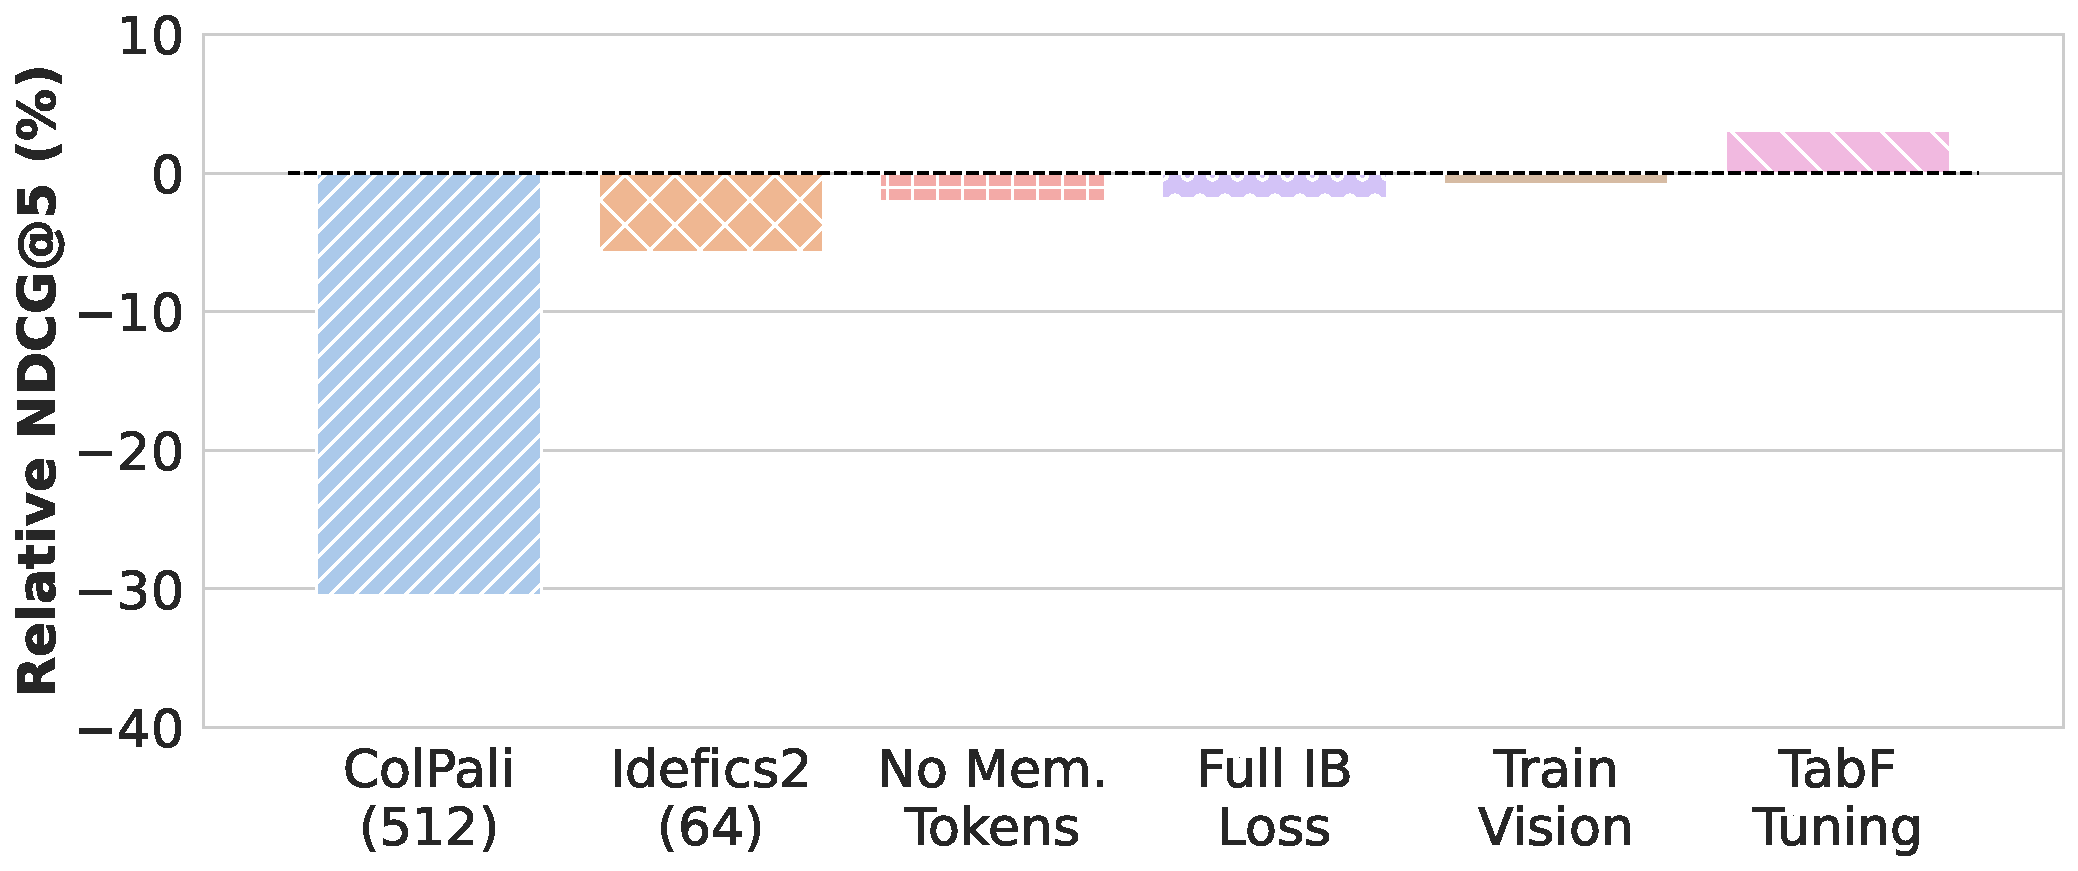
\includegraphics[width = 0.8\linewidth]{images/colpali_images/ablations.pdf}
%     \caption{Relative nDCG@5 performance gain w.r.t. the default \textit{ColPali} (1024 patches). \textit{TabFQuAD fine-tuning} measures the performance difference on the TabFQuAD task after the introduction of targeted data in the training set. All other results refer to performance deltas averaged on all \textit{ViDoRe} tasks.}
%     \label{fig:ablations}
% \end{figure}


\begin{table*}[ht]
    \centering
    
    \resizebox{\textwidth}{!}{%
    \begin{tabular}{ll@{\hskip 0.5em}l@{\hskip 0.5em}l@{\hskip 0.5em}l@{\hskip 0.5em}l@{\hskip 0.5em}l@{\hskip 0.5em}l@{\hskip 0.5em}l@{\hskip 0.5em}l@{\hskip 0.5em}l|@{\hskip 0.5em}l}

    \toprule
     & \textbf{ArxivQ} & \textbf{DocQ} & \textbf{InfoQ} & \textbf{TabF} & \textbf{TATQ} & \textbf{Shift} & \textbf{AI} & \textbf{Energy} & \textbf{Gov.} & \textbf{Health.} & \textbf{Avg.}\\
    \midrule
        ColSigLIP (PaliGemma) & 3.1 & 3.0 & 5.1 & 6.2 & 2.5 & 1.0 & 3.4 & 3.4 & 2.3 & 2.2 & 3.2 \\
        BiSigLIP (PaliGemma) & 18.5 & 14.6 & 33.4 & 39.5 & 16.1 & 5.2 & 27.6 & 32.6 & 36.6 & 35.7 & 26.0 \\
        ColSigLIP (Original) & 2.6 & 2.2 & 2.3 & 5.7 & 1.8 & 1.0 & 2.6 & 4.1 & 1.4 & 1.5 & 2.5 \\
    \midrule
        ColPali (No Q.A. Tokens) & 80.4 & 53.2 & 82.4 & 77.4 & 65.7 & 63.4 & 97.0 & 89.9 & 93.6 & 92.4 & 79.6 \\
        ColPali (Docmatix) & 71.3 & 48.0 & 80.0 & 83.9 & 59.1 & 73.8 & 95.7 & 93.8 & 92.5 & 93.1 & 79.1 \\
        ColPali (224) & 71.0 & 37.4 & 62.3 & 65.7 & 28.6 & 20.4 & 65.7 & 66.8 & 73.9 & 73.0 & 56.5 \\
        ColPali (Vision Trained) & 78.8 & 53.9 & 81.3 & 81.7 & 64.4 & 70.6 & 95.3 & 91.7 & 93.5 & 94.7 & 80.6 \\
        ColPali (No Pairwise) & 79.0 & 53.0 & 82.1 & 85.3 & 63.2 & 66.2 & 94.9 & 88.9 & 92.7 & 92.1 & 79.7 \\
        ColPali (+TabFQuAD training) & 77.6 & 54.7 & 82.6 & 86.5 & 65.4 & 73.9 & 94.8 & 92.4 & \textbf{94.2} & 94.8 & 81.7 \\

        ColIdefics2  (64)      & 73.6 & 48.0 & 82.4 & 81.6 & 63.0 & 57.2 & 95.5 & 86.9 & 86.6 & 91.2 & 76.6 \\
        ColQwen2  (768)         & \textbf{86.4} & \textbf{56.2} & \textbf{89.8} & \textbf{88.7} & \textbf{75.2} & \textbf{85.7} & \textbf{98.8} & \textbf{94.8} & 93.6 & \textbf{97.3} & \textbf{86.6} \\
    \midrule
        \textit{ColPali} (Reference: 448) & 79.1 & 54.4 & 81.8 & 83.9 & 65.8 & 73.2 & 96.2 & 91.0 & 92.7 & 94.4 & 81.3 \\
            \bottomrule
    \end{tabular}
    }
    

    \caption[\textsc{ViDoRe} ablations and negative results]{\textbf{Benchmark scores for the ``negative results" and various ablations on \textsc{ViDoRe}; \textit{ColPali} for reference.} Results are presented using nDCG@5 metrics. Text-only metrics are not computed for benchmarks with only visual elements.}
    \label{table:negative_results}
\end{table*}





\newpage
\section{More similarity maps}
\label{section:more_similarity_maps}
In \autoref{fig:similarity_map_kazakhstan}, \textit{ColPali} assigns a high similarity to all patches with the word \textit{``Kazakhstan"} when given the token \texttt{<\_Kazakhstan>}. Moreover, our model seems to exhibit world knowledge capabilities as the patch around the word \textit{"Kashagan"}—an offshore oil field in Kazakhstan—also shows a high similarity score.

\begin{figure}
\centering
    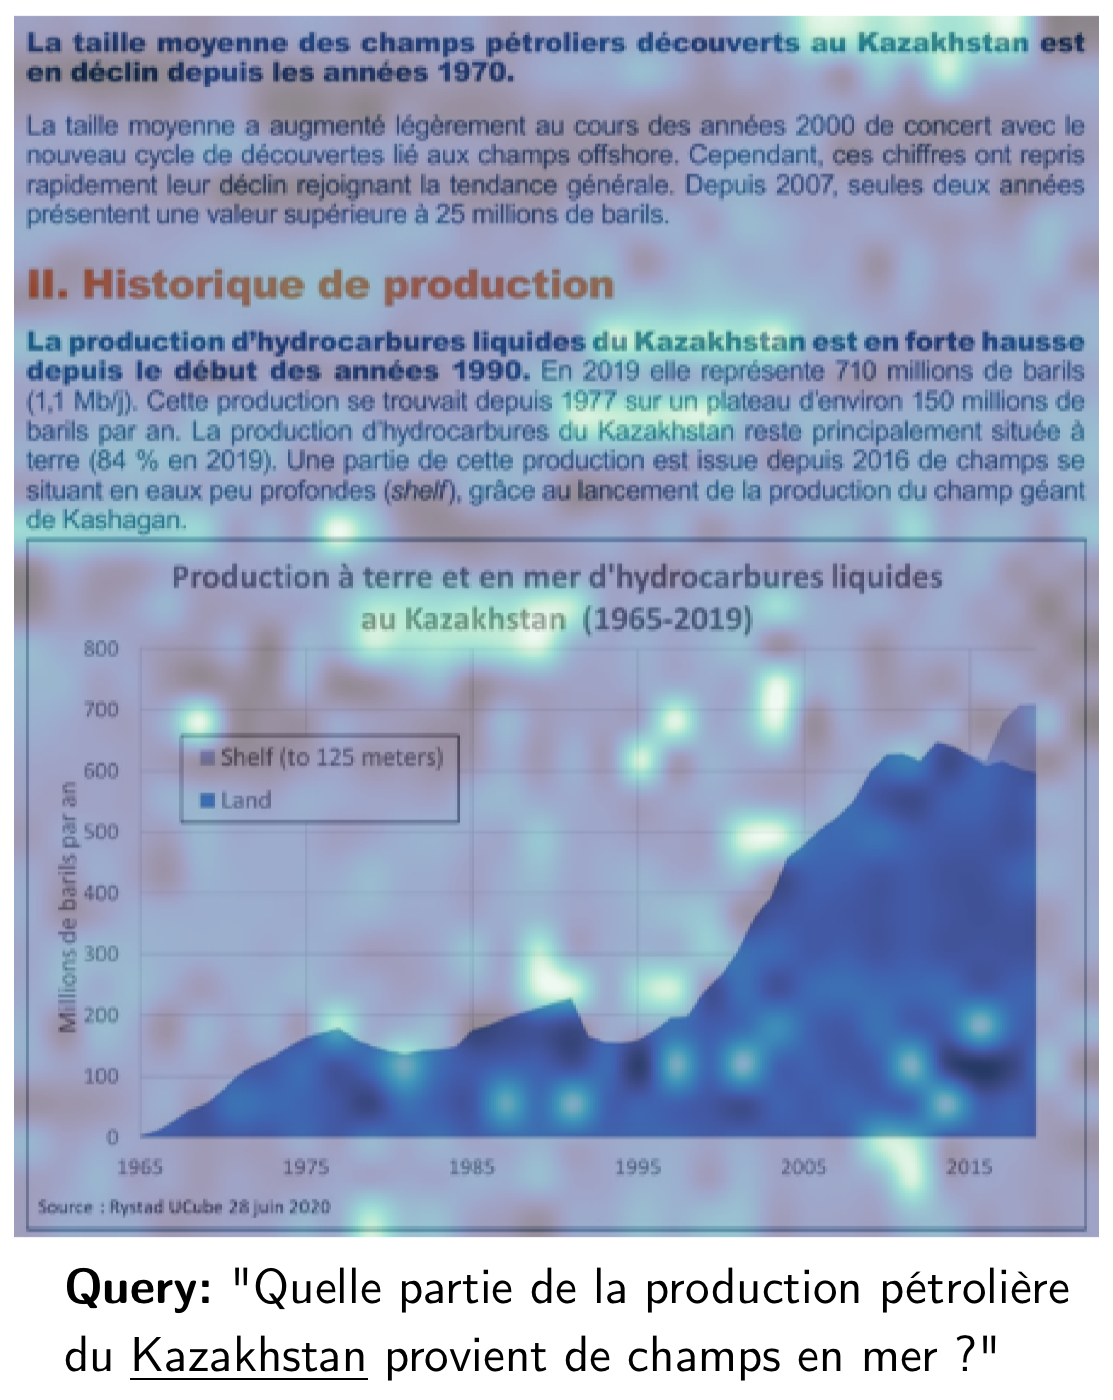
\includegraphics[width=0.5\linewidth]{images/colpali_images/similarity_maps/similarity_map_kazakhstan.png} 
    \caption[Similarity map example]{Similarity of the image patches w.r.t. the underlined token in the user query. This example is from the \textit{Shift} test set.}
\label{fig:similarity_map_kazakhstan}
\end{figure}

It is also interesting to highlight that both this similarity map and the one displayed in \autoref{fig:similarity-maps} showcase a few white patches with high similarity scores. This behavior might first seem surprising as the white patches should not carry a meaningful signal from the original images. We believe the vectors associated with these patches share a similar role with the ViT registers \sidecite{darcet_vision_2023}, i.e.\ these patches were repurposed for internal computations and stored the global information from the whole image.

\section{Model glossary}
\label{section:model_glossary}


\subsection*{SigLIP}
\label{subsection:glossary_siglip}

SigLIP (Sigmoid Loss for Language Image Pre-Training) builds upon CLIP (Contrastive Language-Image Pretraining)—a foundational model that aligns images and text by maximizing the similarity between correct image-text pairs while minimizing it for incorrect ones, leveraging a contrastive loss \sidecite{zhai_sigmoid_2023}. Unlike CLIP \sidecite{radford_learning_2021}, which applies the softmax function to the logits, SigLIP uses the sigmoid activation function. This innovation eliminates the need for a global view of all pairwise similarities between images and texts within a batch, enabling more flexible batch size scaling (up to 1M items per batch, with an effective optimal batch size of 32k). This approach allows SigLIP to achieve state-of-the-art performance in zero-shot image classification tasks.


\subsection*{PaliGemma}
\label{subsection:glossary_paligemma}

PaliGemma is a 3B-parameter vision-language model. It integrates the SigLIP vision encoder with a Gemma-2B language decoder, connected via a multimodal linear projection layer \sidecite{lucas_beyer_paligemma_2024}. The model processes images by segmenting them into a fixed number of Vision Transformer \sidecite{dosovitskiy_image_2020} tokens, which are prepended to an optional text prompt.

A distinguishing feature of PaliGemma is its operation as a Prefix-Language Model (Prefix-LM). This design ensures full attention between image tokens and the user-provided input (prefix) while generating outputs auto-regressively (suffix). This architecture allows image tokens to access the task-specific query during processing, facilitating more effective task-dependent reasoning.

PaliGemma was trained in four stages: unimodal pretraining with existing components, extended multimodal pretraining, short high-resolution pretraining, and task-specific fine-tuning.


\subsection*{ColBERT}
\label{subsection:glossary_colbert}

ColBERT (Contextualized Late Interaction over BERT) is a retrieval model designed to balance speed and effectiveness in information retrieval tasks \sidecite{khattab2020colbert}. Traditional retrieval models are typically categorized based on their type of interaction: either processing queries and documents independently for efficiency (bi-encoders) or jointly to capture rich contextual relationships (cross-encoders). ColBERT combines the advantages of both approaches through a novel late interaction mechanism.

Queries and documents are encoded separately using BERT, enabling offline pre-computation of document representations for scalability. Instead of pooling embeddings into a single vector, ColBERT retains token-level embeddings and employs a MaxSim operator to compute fine-grained similarity scores. For each query token, the model determines the maximum similarity with document tokens, summing these scores to compute relevance.

This architecture preserves the contextual richness of deep language models while significantly improving computational efficiency. By delaying the interaction step, ColBERT supports vector similarity indexing, facilitating end-to-end retrieval from large collections without prohibitive costs. Empirical evaluations on passage search datasets demonstrate that ColBERT achieves competitive effectiveness compared to existing BERT-based models \sidecite{devlin2019bert}, while executing queries orders of magnitude faster and with drastically reduced computational requirements.


\newpage
\section{Examples from the \textsc{ViDoRe} benchmark}
\label{subsection:docvisbenchmark_examples}

\vspace*{3\baselineskip}

\begin{center}
    \textbf{Energy} \\[1ex]
    \begin{figure}[h]
        \centering
        \begin{subfigure}[t]{0.30\textwidth}
            \caption*{\textbf{Query}: What types of accounts or products allow investors to defer paying taxes?}
            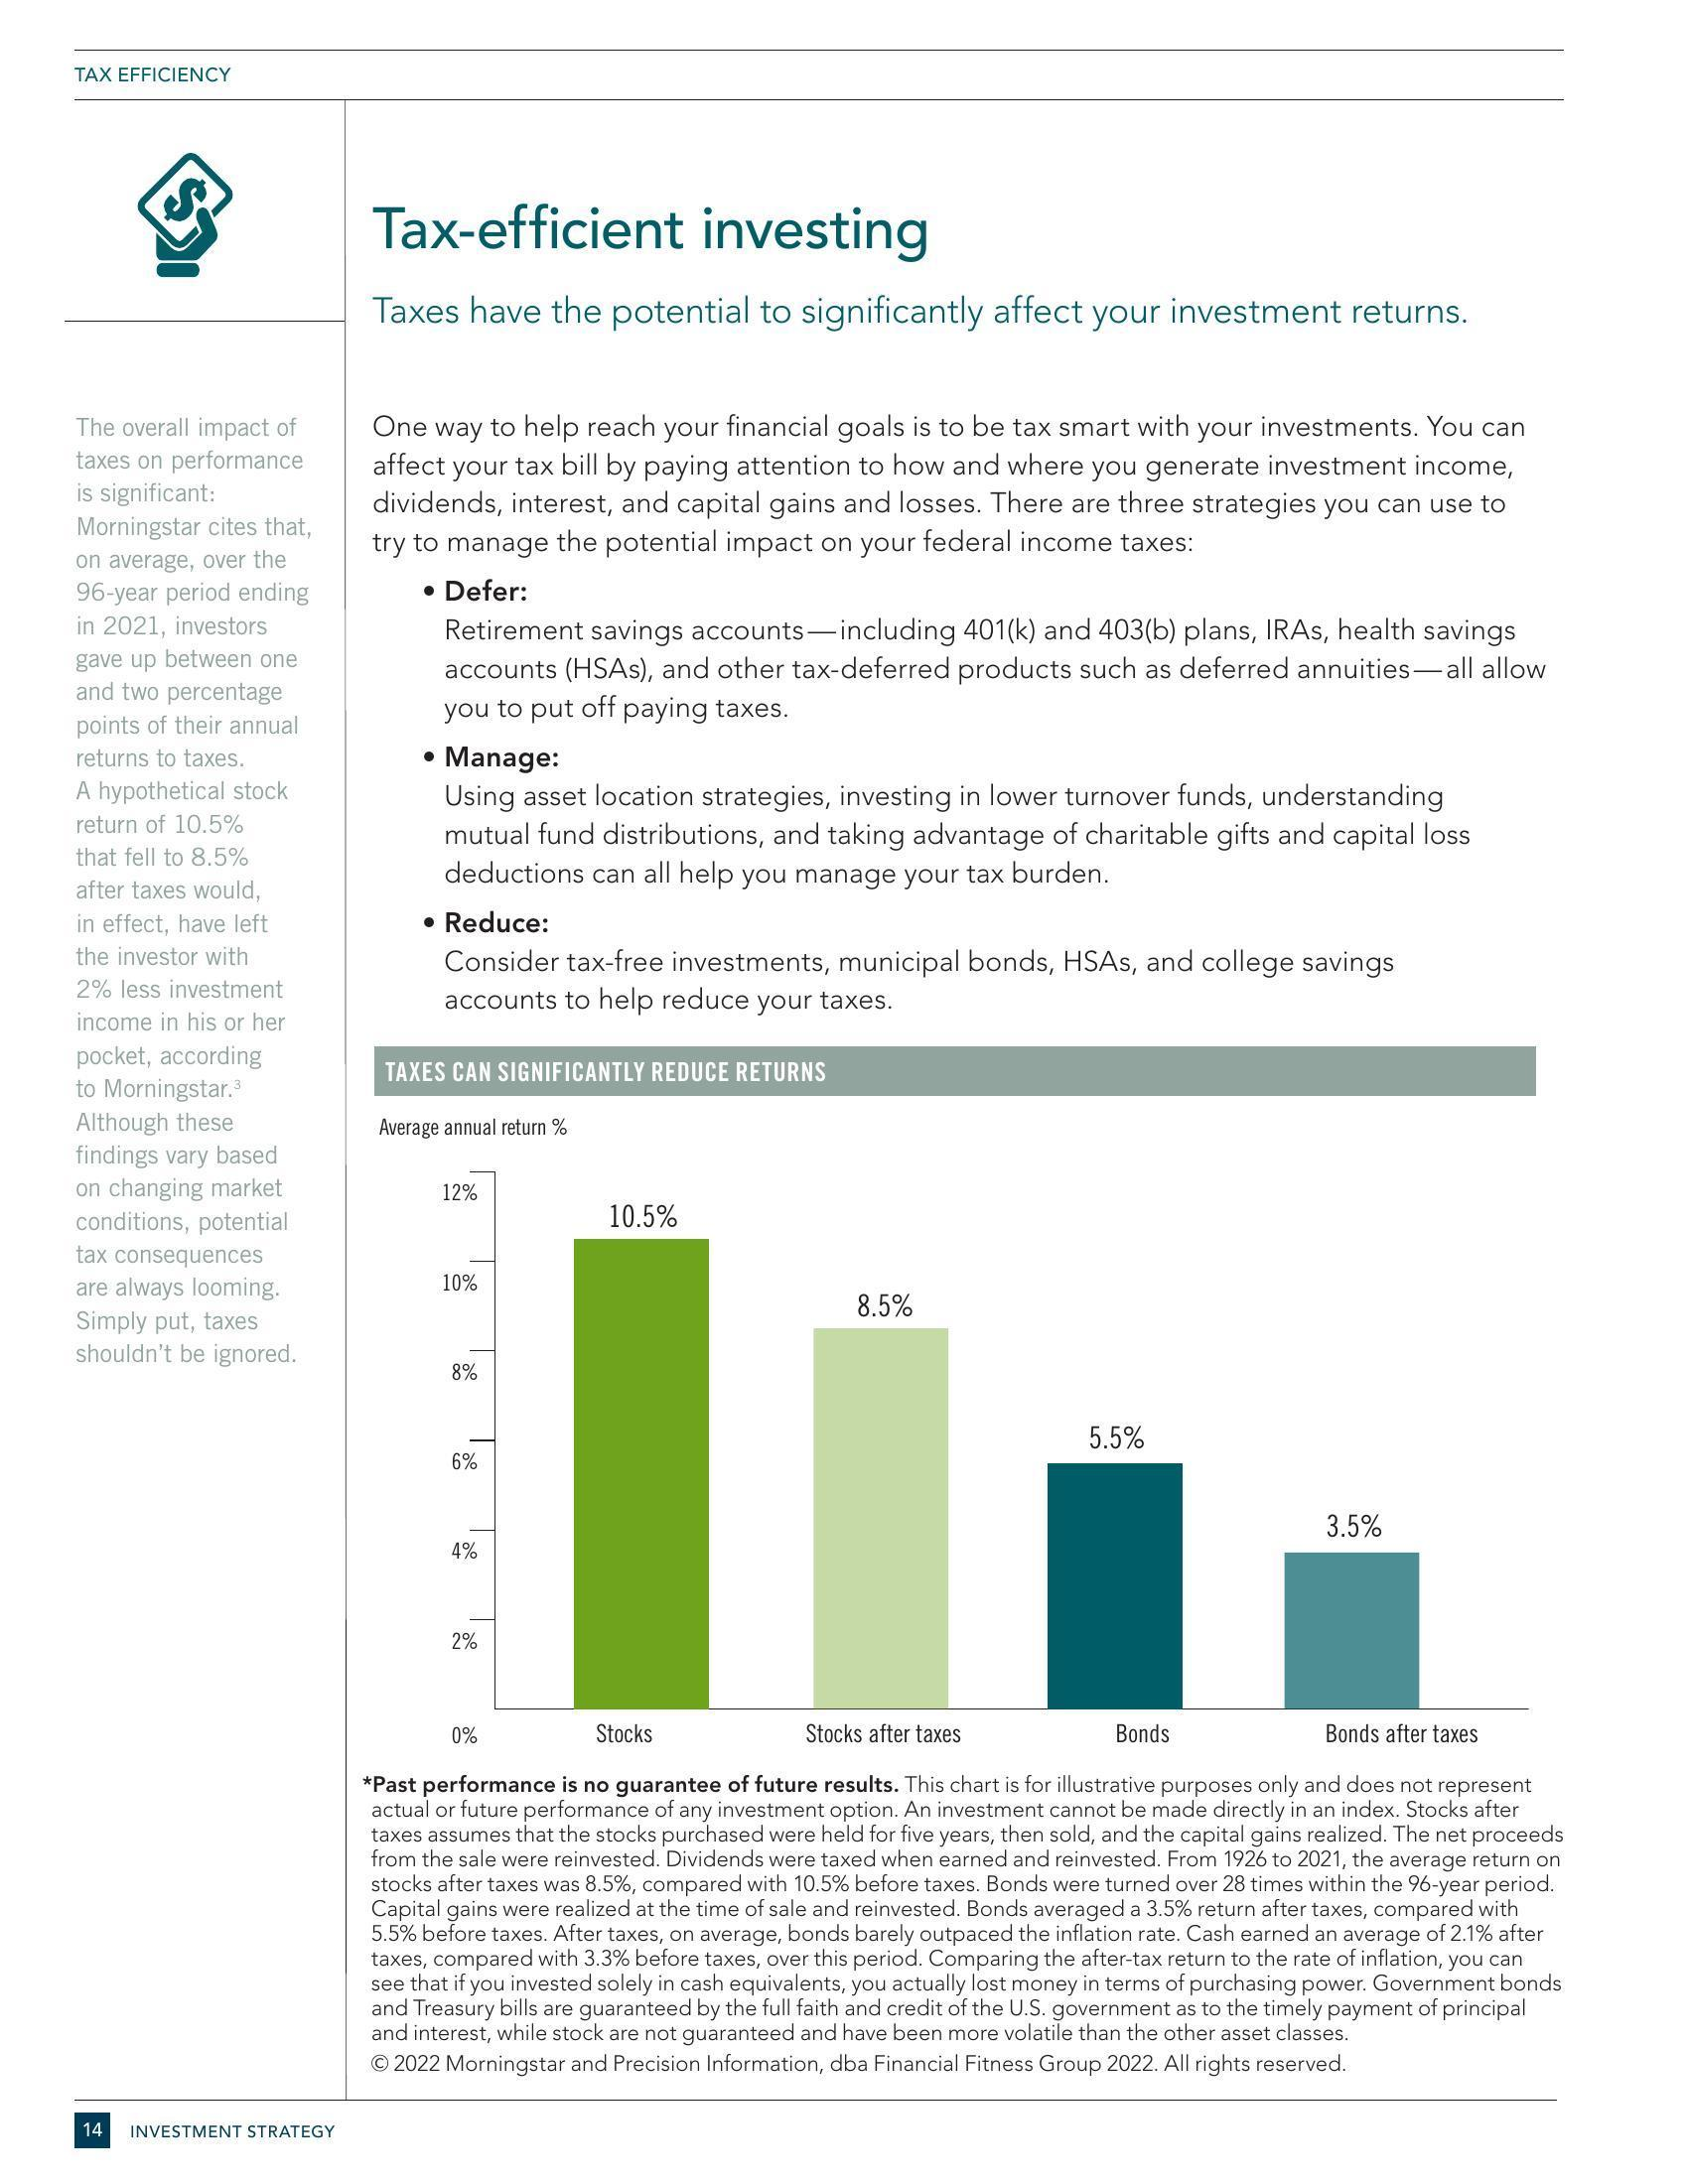
\includegraphics[width=\textwidth]{images/colpali_images/dataset_samples/energy_1.jpeg}
        \end{subfigure} \ 
        \begin{subfigure}[t]{0.30\textwidth}
            \caption*{\textbf{Query}: What is the estimated total savings for a PV system in Durham under the net metering (flat rate) billing option over the system's useful life of 25 years?}
            \includegraphics*[width=\textwidth]{images/colpali_images/dataset_samples/energy_2.jpeg}
        \end{subfigure}
        \begin{subfigure}[t]{0.30\textwidth}
            \caption*{\textbf{Query}: What is the projected peak electricity demand in California for the year 2030?}
            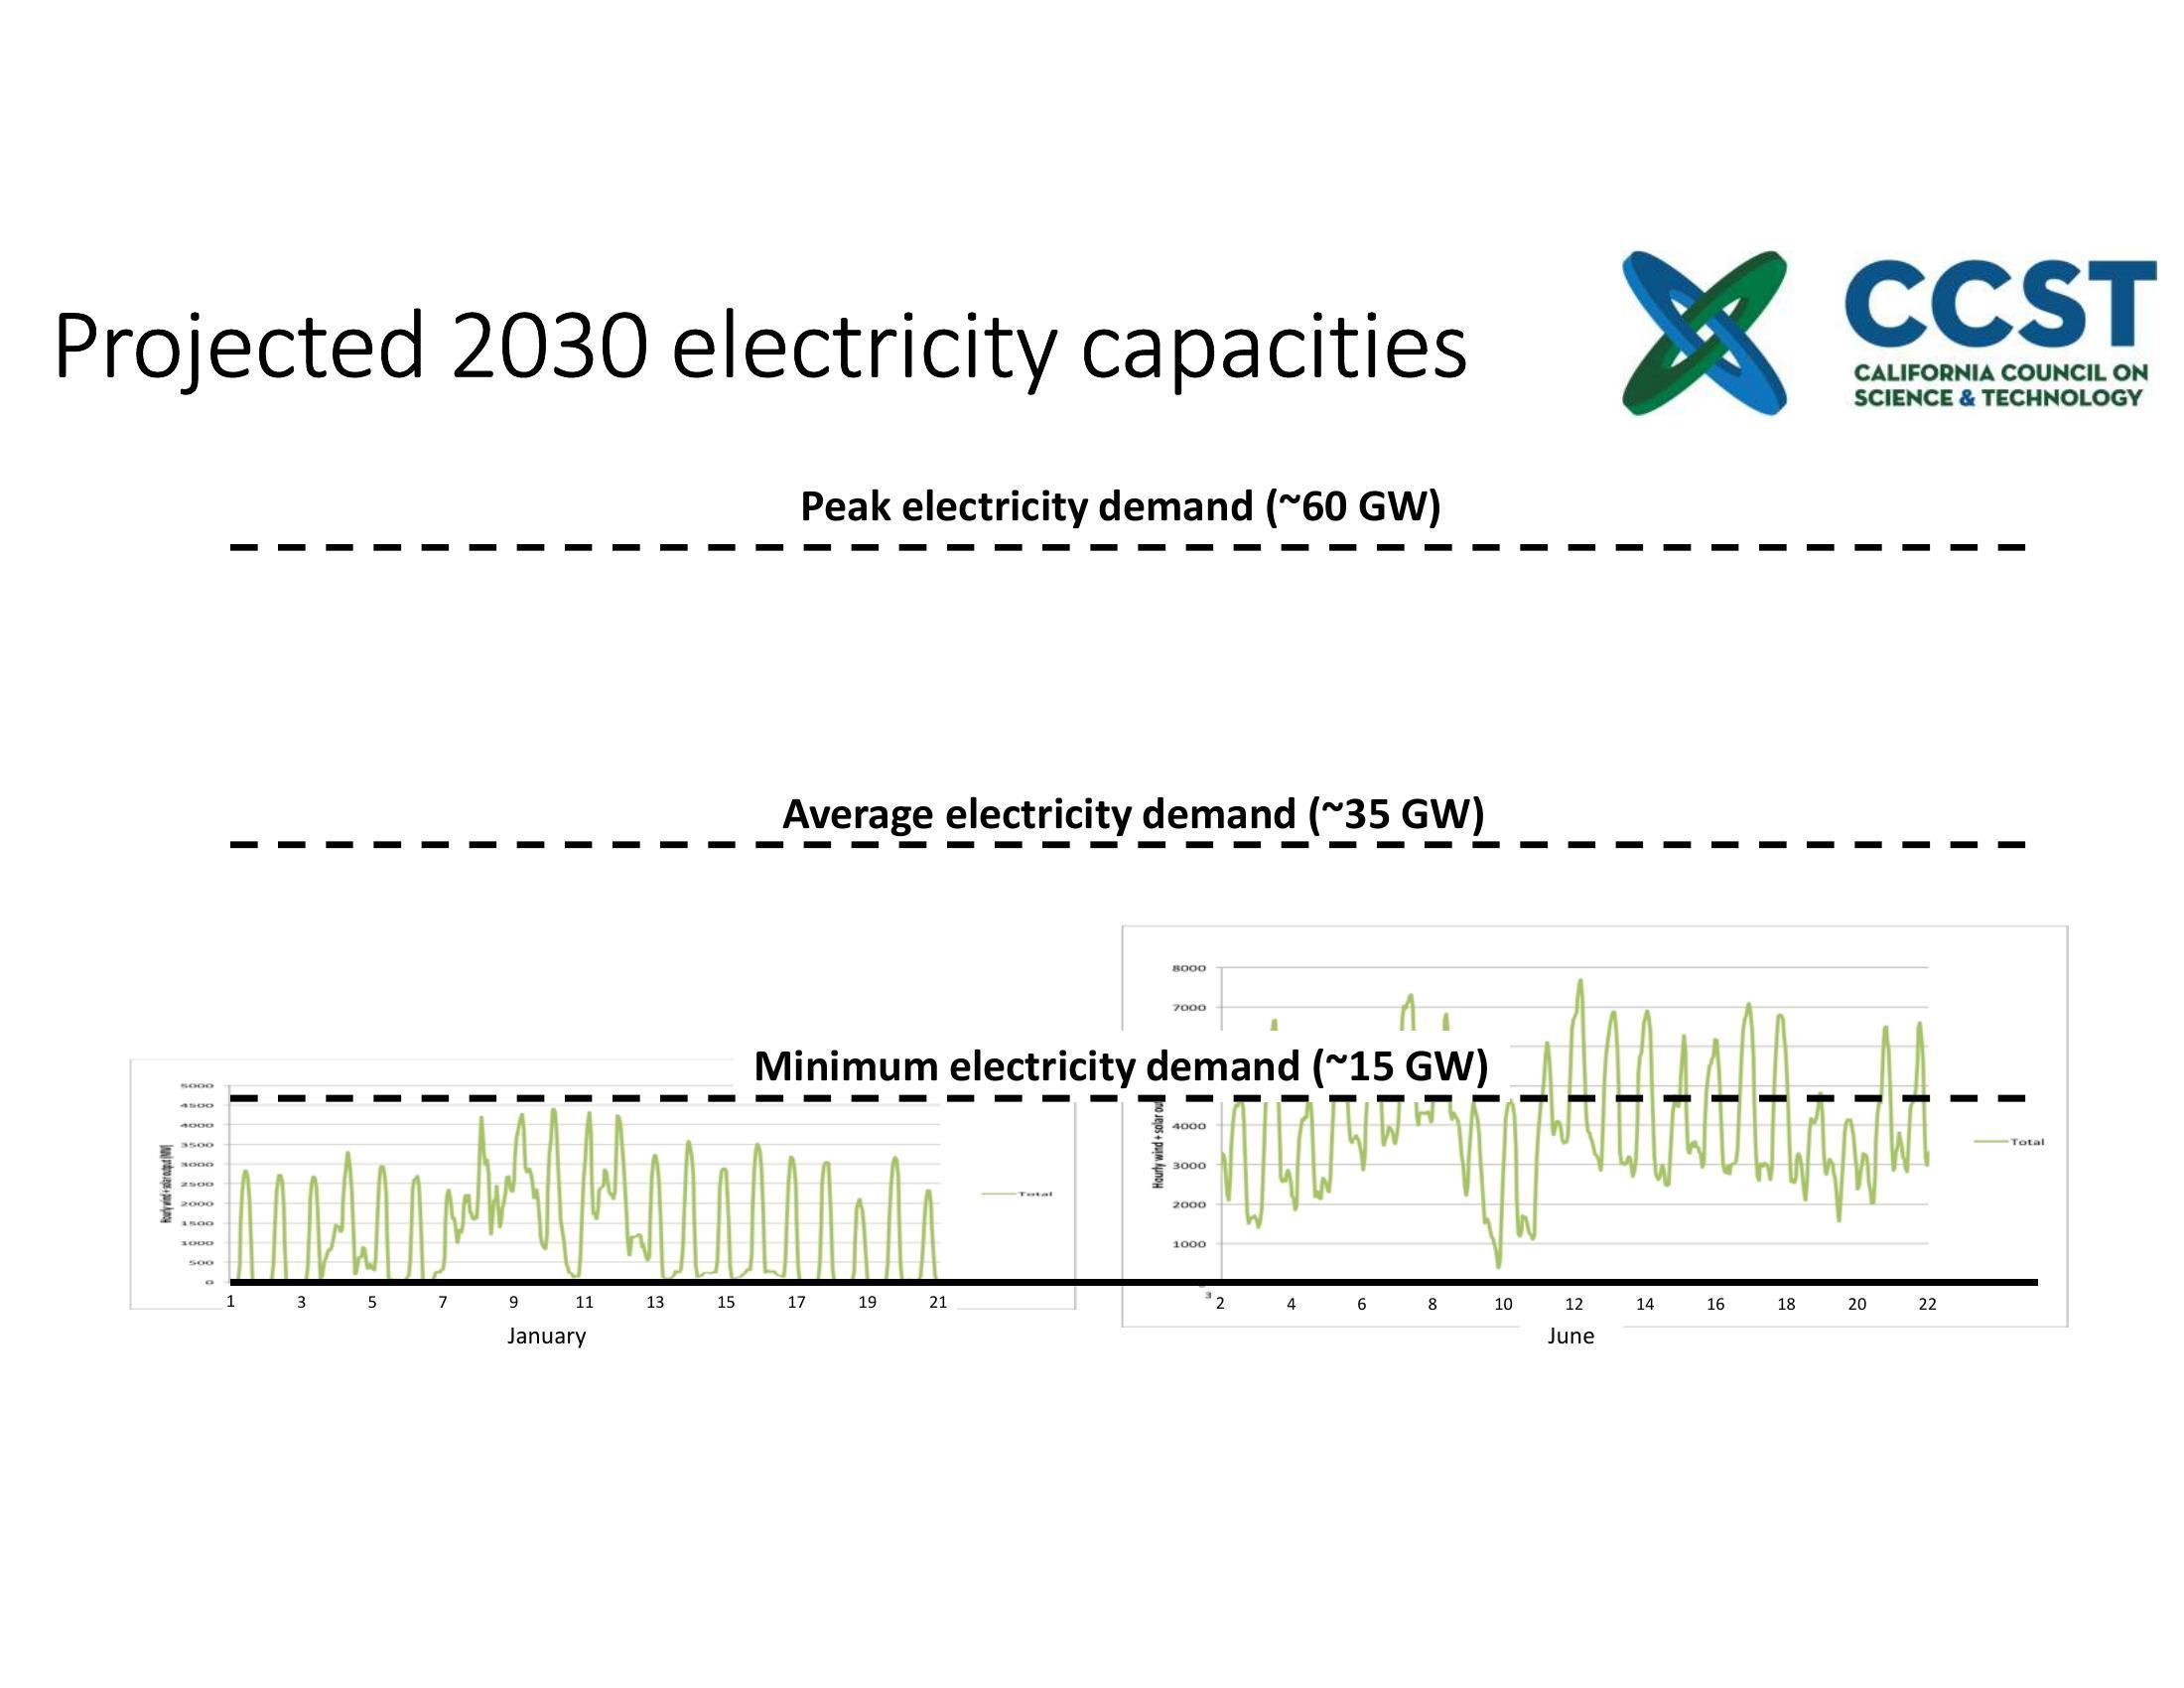
\includegraphics[width=\textwidth]{images/colpali_images/dataset_samples/energy_3.jpeg}
        \end{subfigure} \ 
    \end{figure}

    \vspace*{5\baselineskip}
    
    \textbf{Artificial Intelligence} \\[1ex]
    \begin{figure}[h]
        \centering
        \begin{subfigure}[t]{0.30\textwidth}
            \caption*{\textbf{Query}: What are some common outcome areas targeted by TAII for different age groups?}
            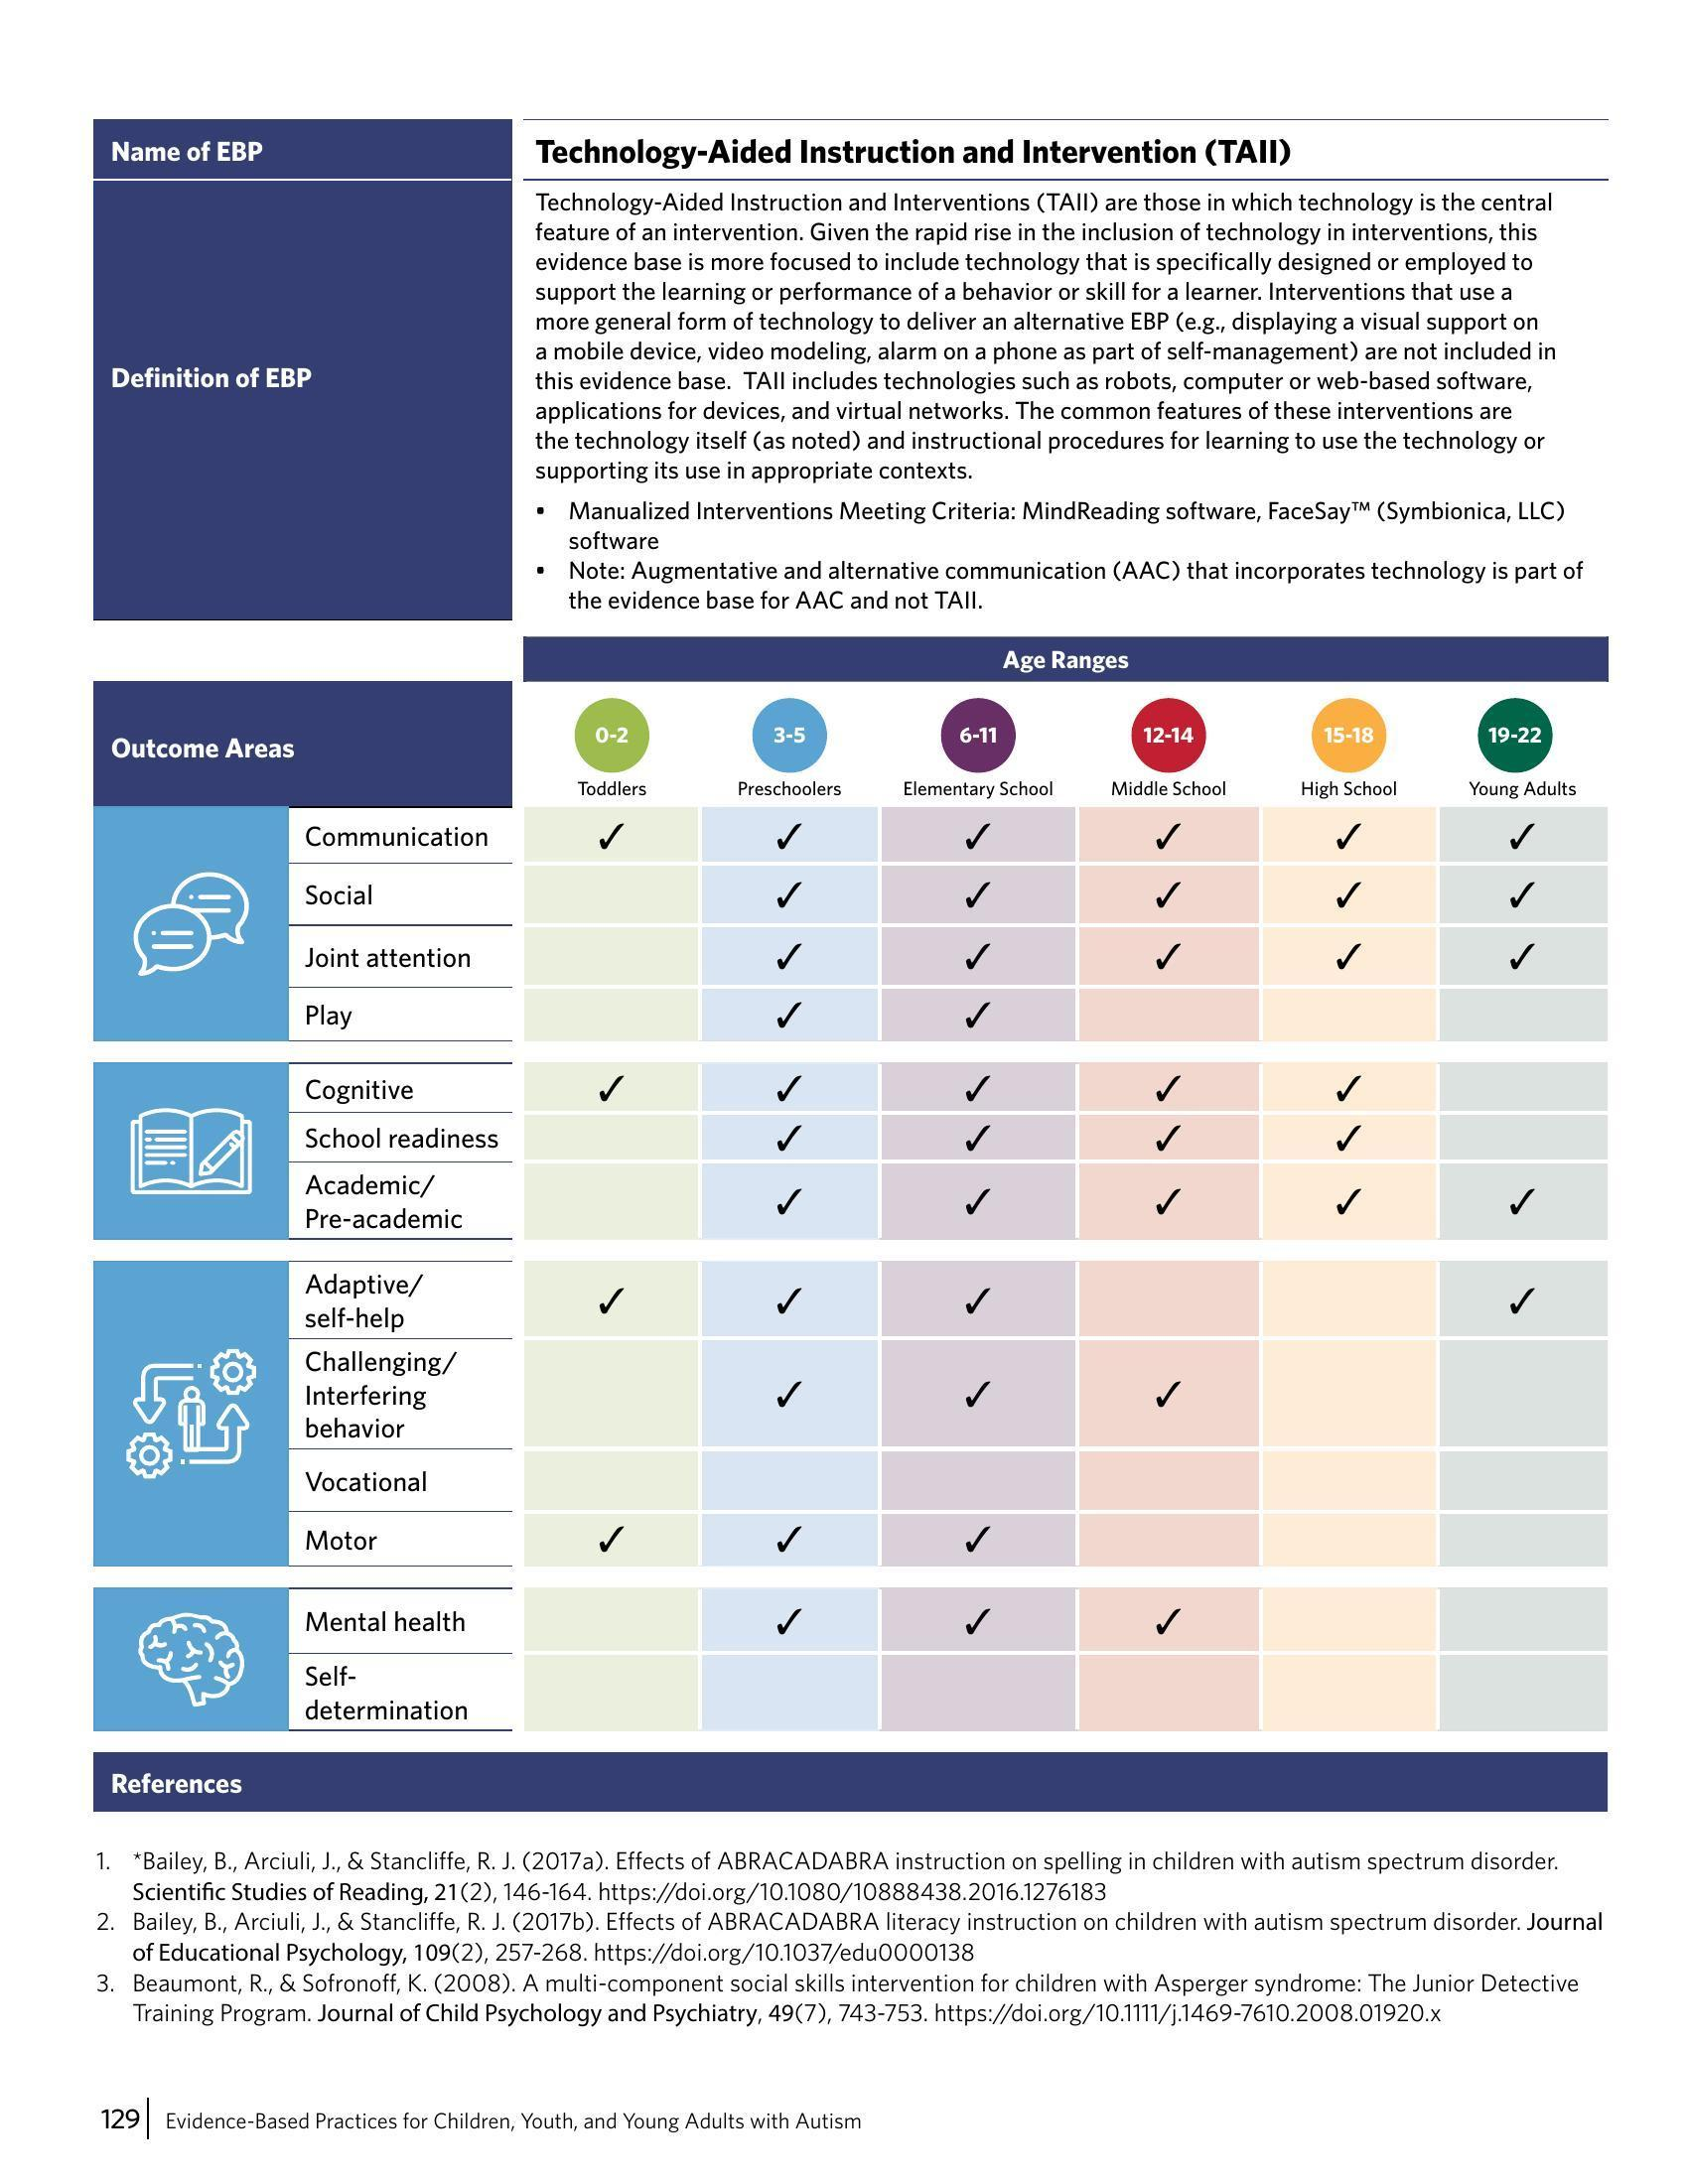
\includegraphics[width=\textwidth]{images/colpali_images/dataset_samples/ai_1.jpeg}
        \end{subfigure} \ 
        \begin{subfigure}[t]{0.30\textwidth}
            \caption*{\textbf{Query}: What did the robot monitor to determine when to activate or deactivate the blower motor and blinker?}
            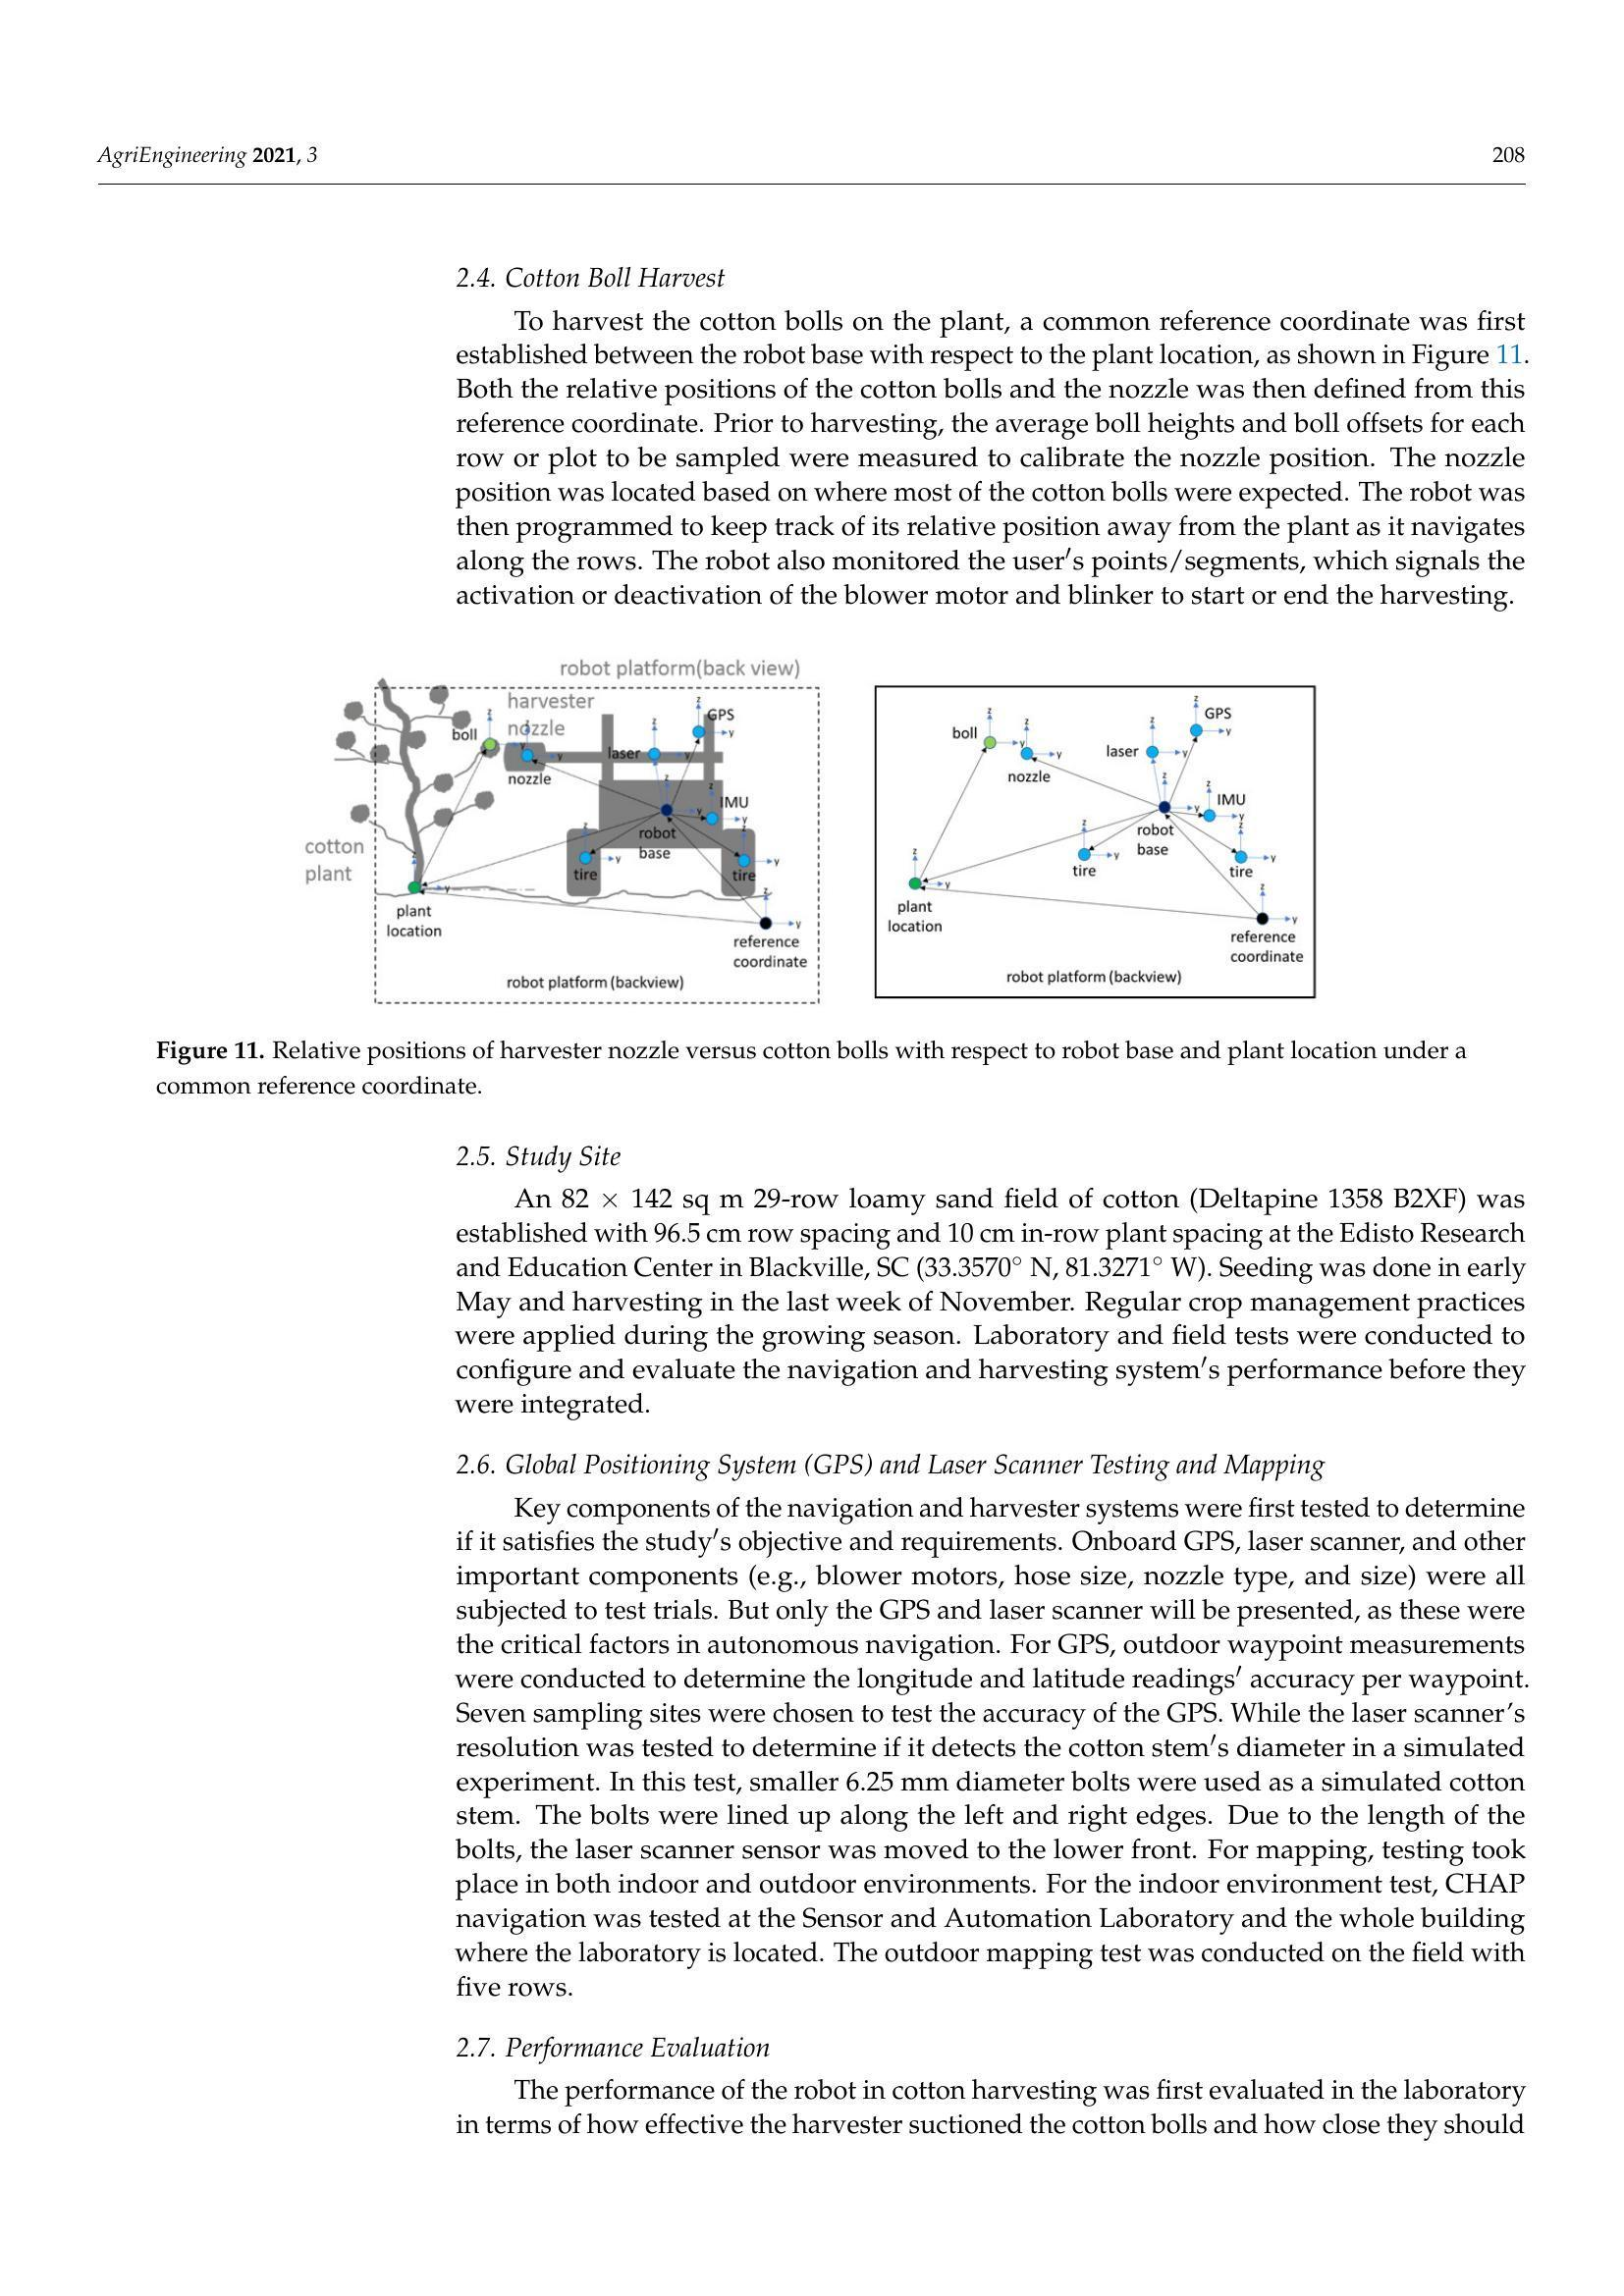
\includegraphics[width=\textwidth]{images/colpali_images/dataset_samples/ai_2.jpeg}
        \end{subfigure} \ 
        \begin{subfigure}[t]{0.30\textwidth}
            \caption*{\textbf{Query}: What is the key approach used in the PDP architecture?}
            \includegraphics*[width=\textwidth]{images/colpali_images/dataset_samples/ai_3.jpeg}
        \end{subfigure}
    \end{figure}

    \newpage
    \vspace*{3\baselineskip}

    \textbf{Healthcare Industry} \\[1ex]
    \begin{figure}[h]
        \centering
        \begin{subfigure}[t]{0.30\textwidth}
            \caption*{\textbf{Query}: What is the chemical formula for the ferroelectric material Lead Zirconium Titanate (PZT)?}
            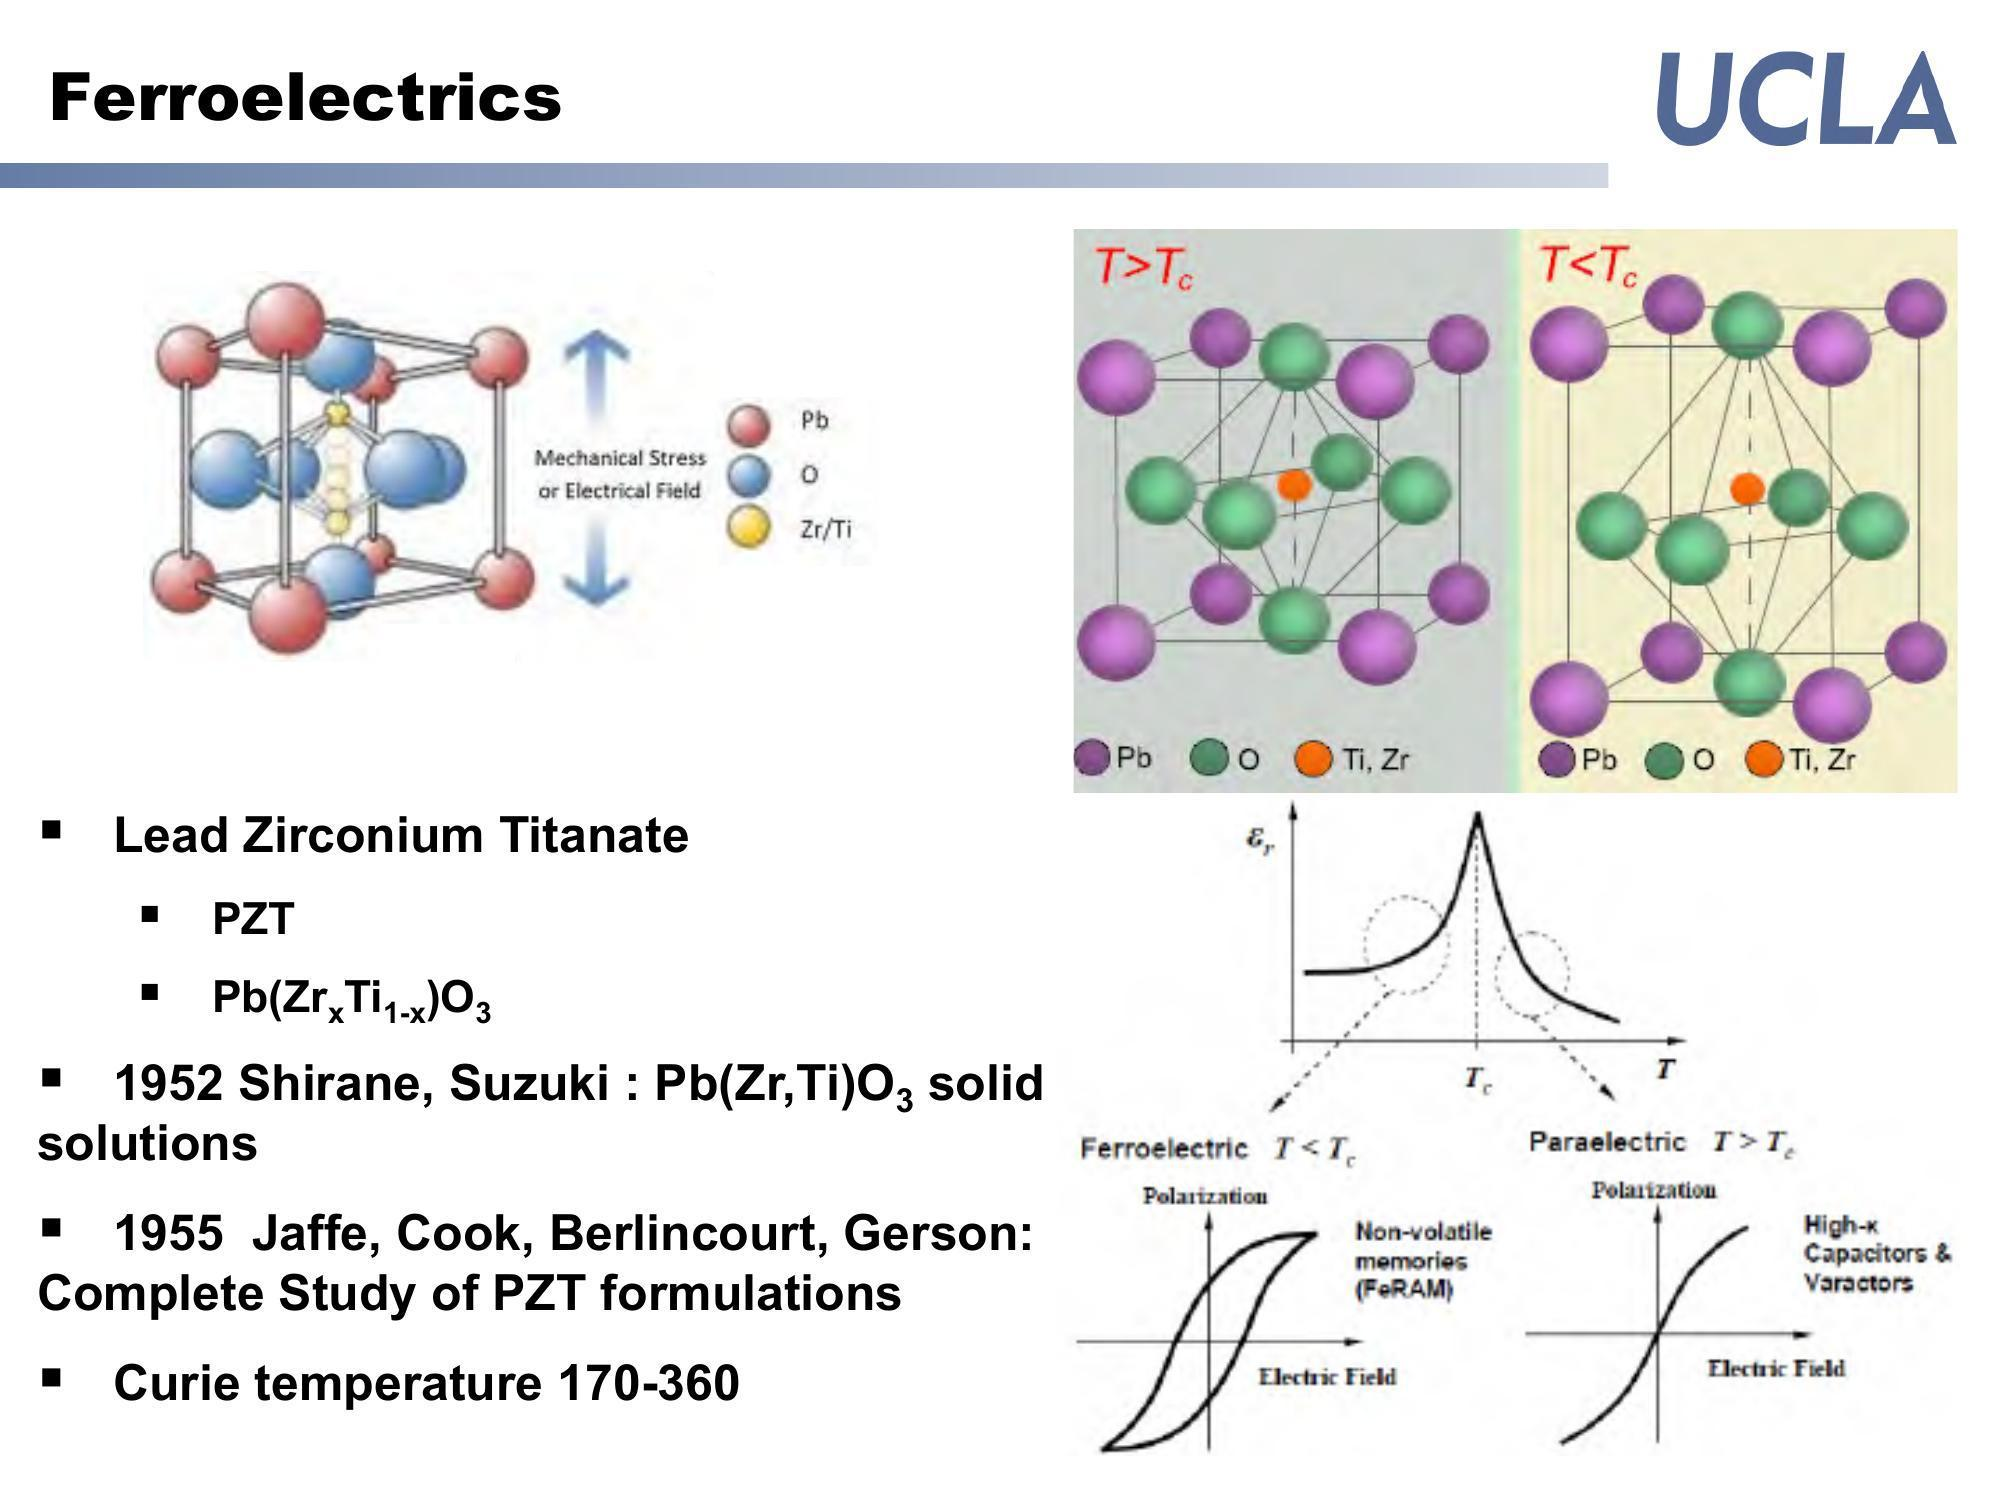
\includegraphics[width=\textwidth]{images/colpali_images/dataset_samples/healthcare_1.jpeg}
        \end{subfigure} \ 
        \begin{subfigure}[t]{0.30\textwidth}
            \caption*{\textbf{Query}: What government entities are involved in public financing for healthcare in the US?}
            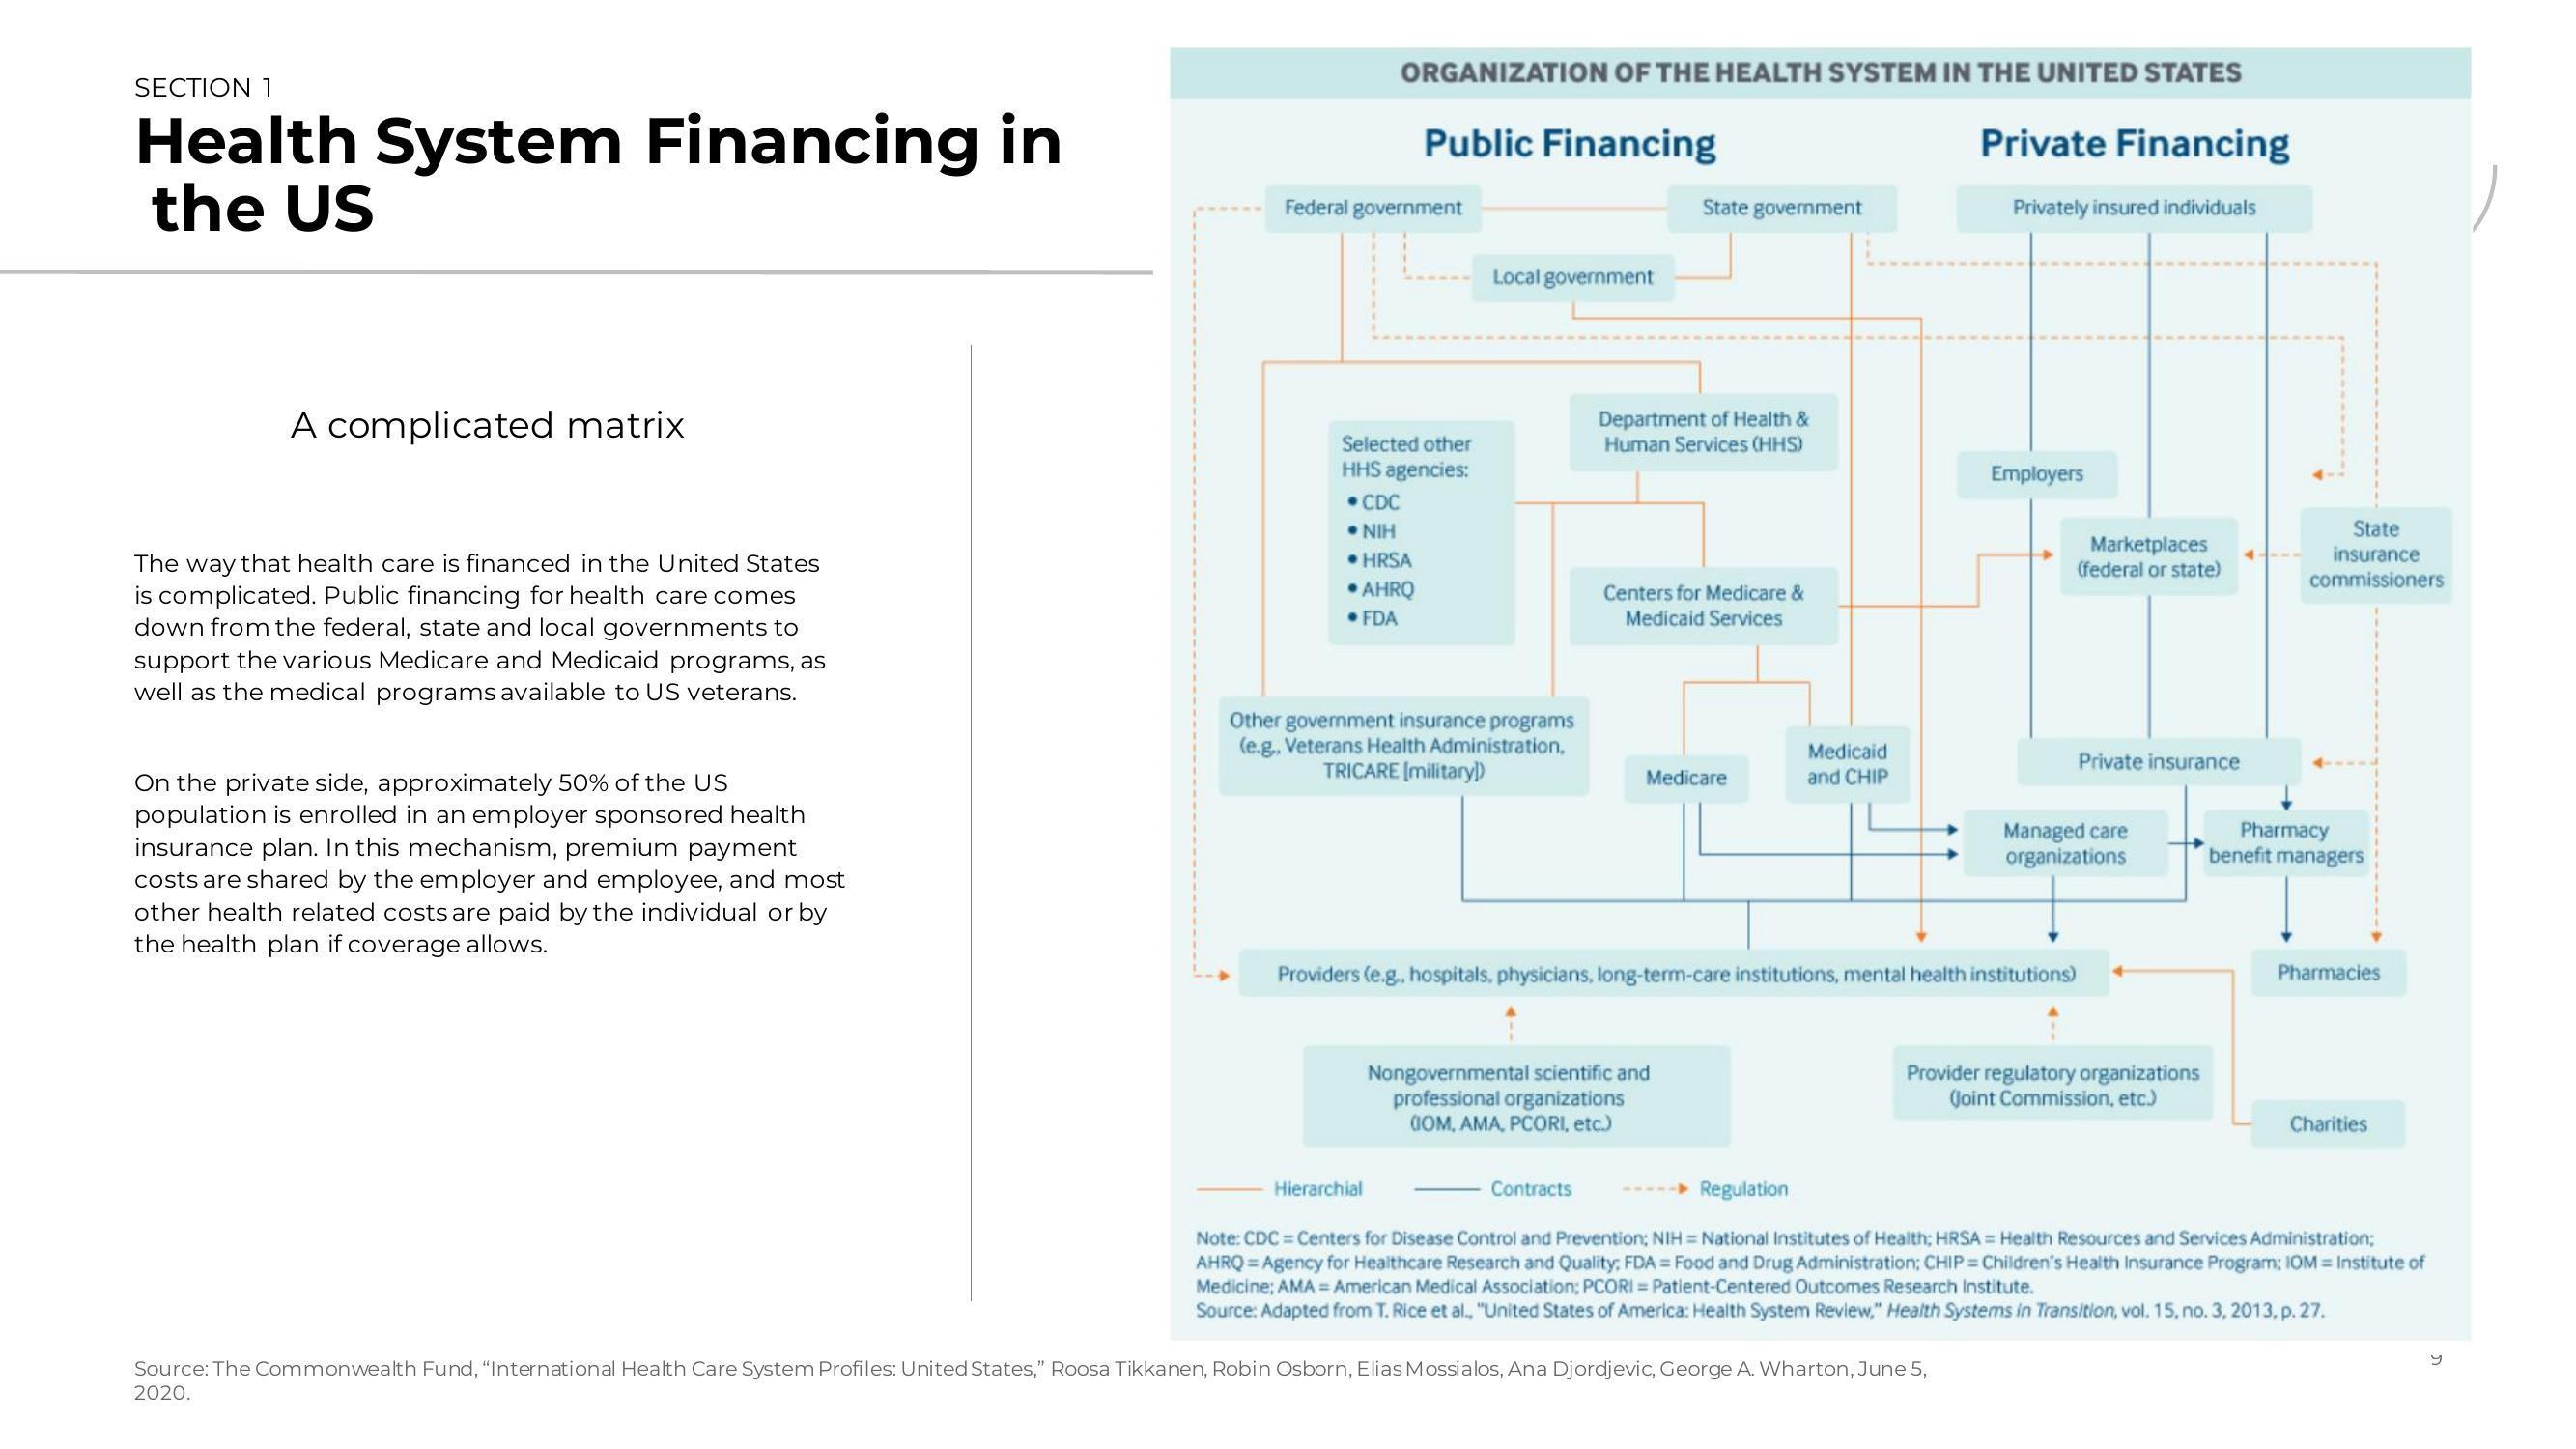
\includegraphics[width=\textwidth]{images/colpali_images/dataset_samples/healthcare_2.jpeg}
        \end{subfigure} \ 
        \begin{subfigure}[t]{0.30\textwidth}
            \caption*{\textbf{Query}: What does the AVPU scale stand for in assessing the level of consciousness of a seriously ill child?}
            \includegraphics*[width=\textwidth]{images/colpali_images/dataset_samples/healthcare_3.jpeg}
        \end{subfigure}
    \end{figure}

    \vspace*{5\baselineskip}

    \textbf{Government Reports} \\[1ex]
    \begin{figure}[h]
        \centering
        \begin{subfigure}[t]{0.30\textwidth}
            \caption*{\textbf{Query}: What are some mandates for the EPA under the Pollution Prevention Act?}
            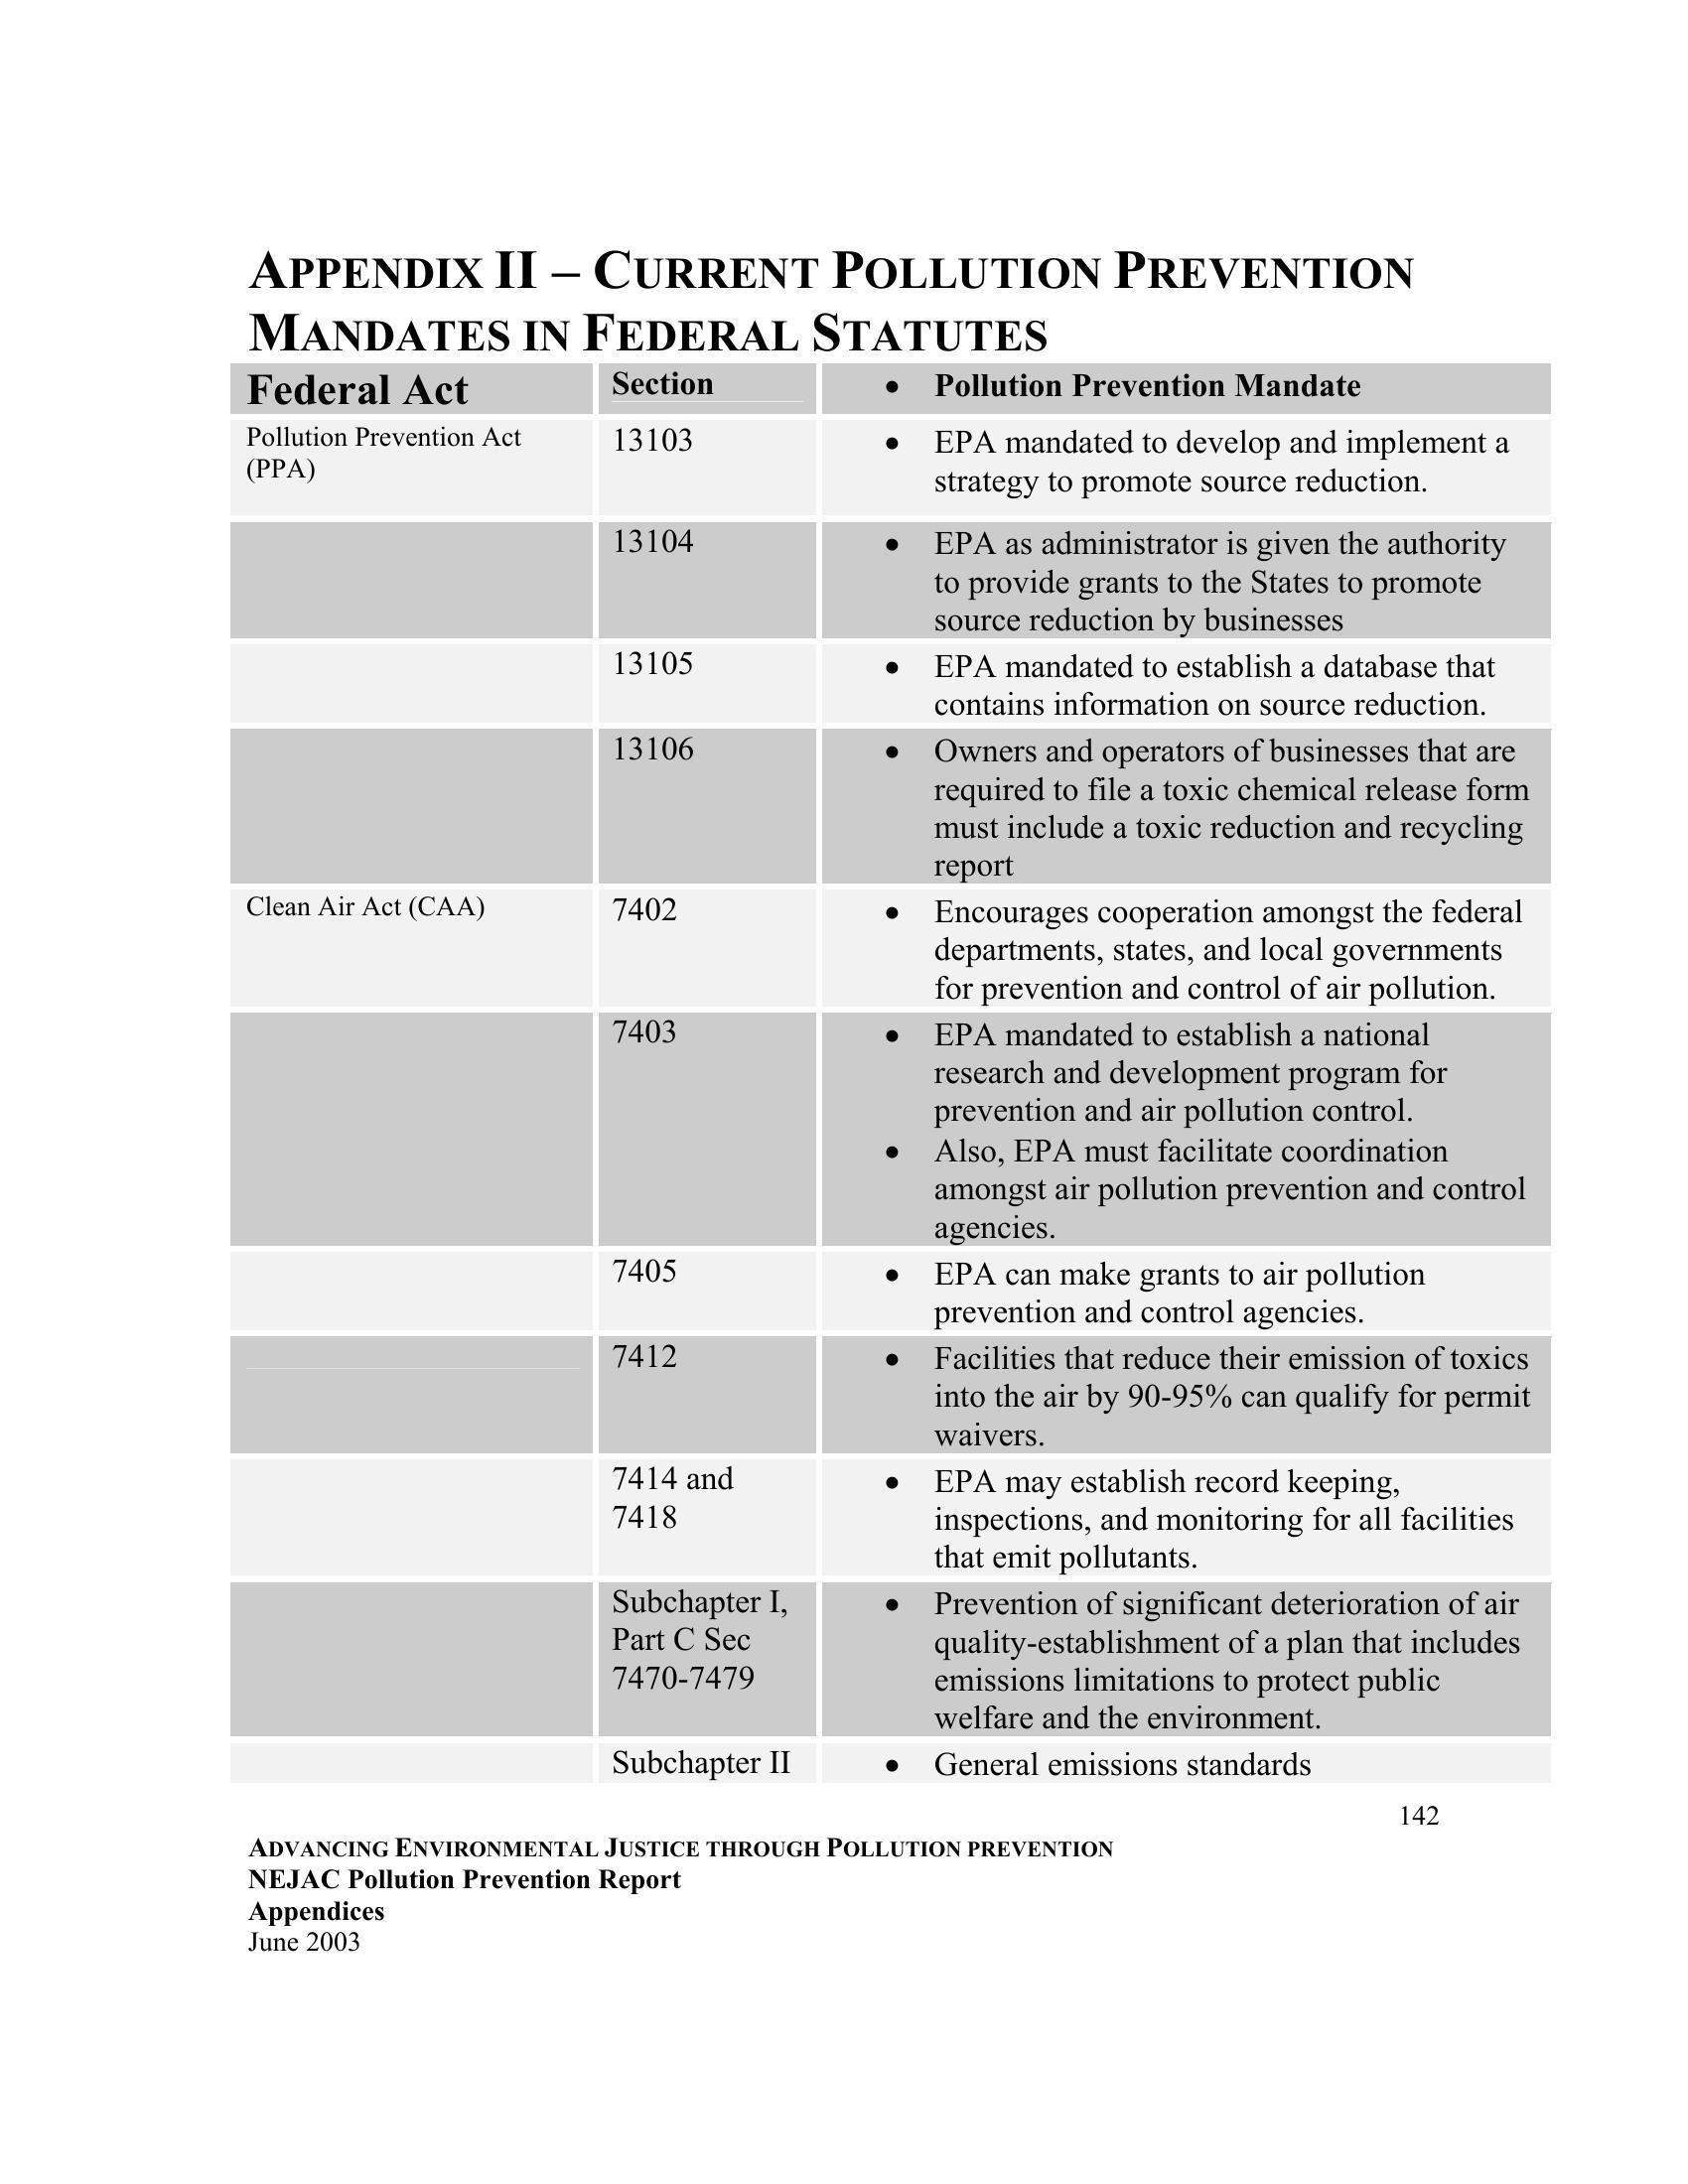
\includegraphics[width=\textwidth]{images/colpali_images/dataset_samples/gov_1.jpeg}
        \end{subfigure} \ 
        \begin{subfigure}[t]{0.30\textwidth}
            \caption*{\textbf{Query}: What is the strategy of KPMG Hazem Hassan?}
            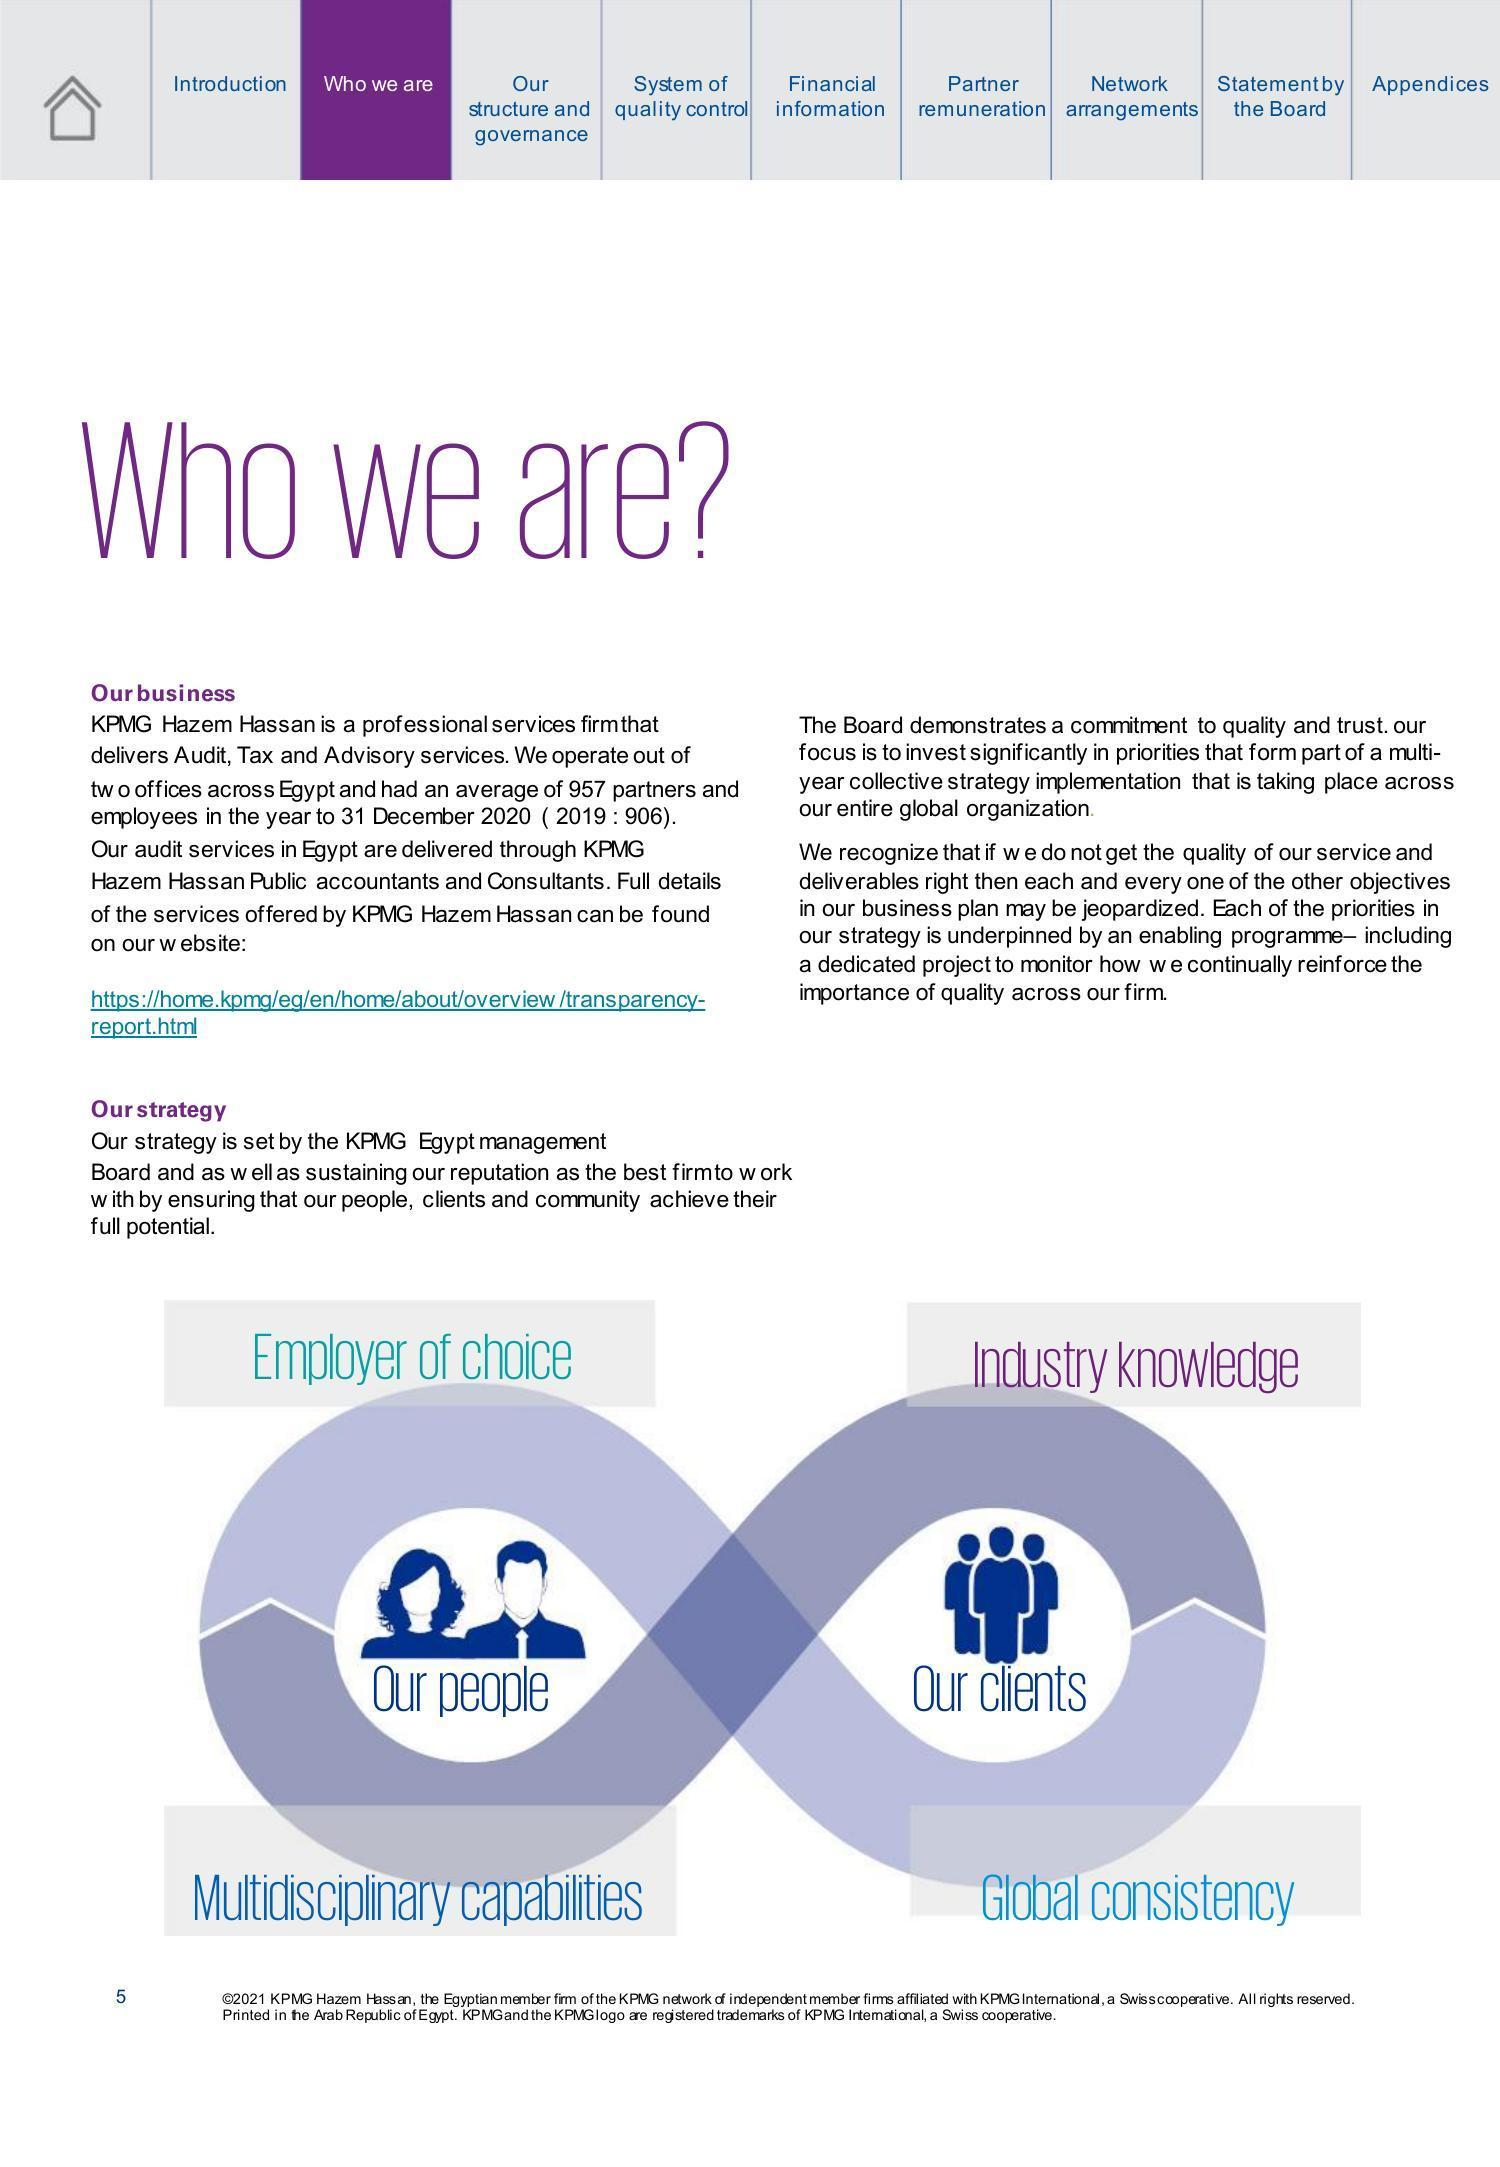
\includegraphics[width=\textwidth]{images/colpali_images/dataset_samples/gov_2.jpeg}
        \end{subfigure} \ 
        \begin{subfigure}[t]{0.30\textwidth}
            \caption*{\textbf{Query}: What is the trust signal score for the consumer industry best-in-class archetype?}
            \includegraphics*[width=\textwidth]{images/colpali_images/dataset_samples/gov_3.jpeg}
        \end{subfigure}
    \end{figure}

    \newpage
    \vspace*{3\baselineskip}

    \textbf{Shift} \\[1ex]
    \begin{figure}[h]
        \centering
        \begin{subfigure}[t]{0.30\textwidth}
            \caption*{\textbf{Query}: Selon le graphique, quelle est la capacité d'import et la consommation réelle de carburants SAF (biocarburants durables pour l'aviation) prévues en 2050 ?}
            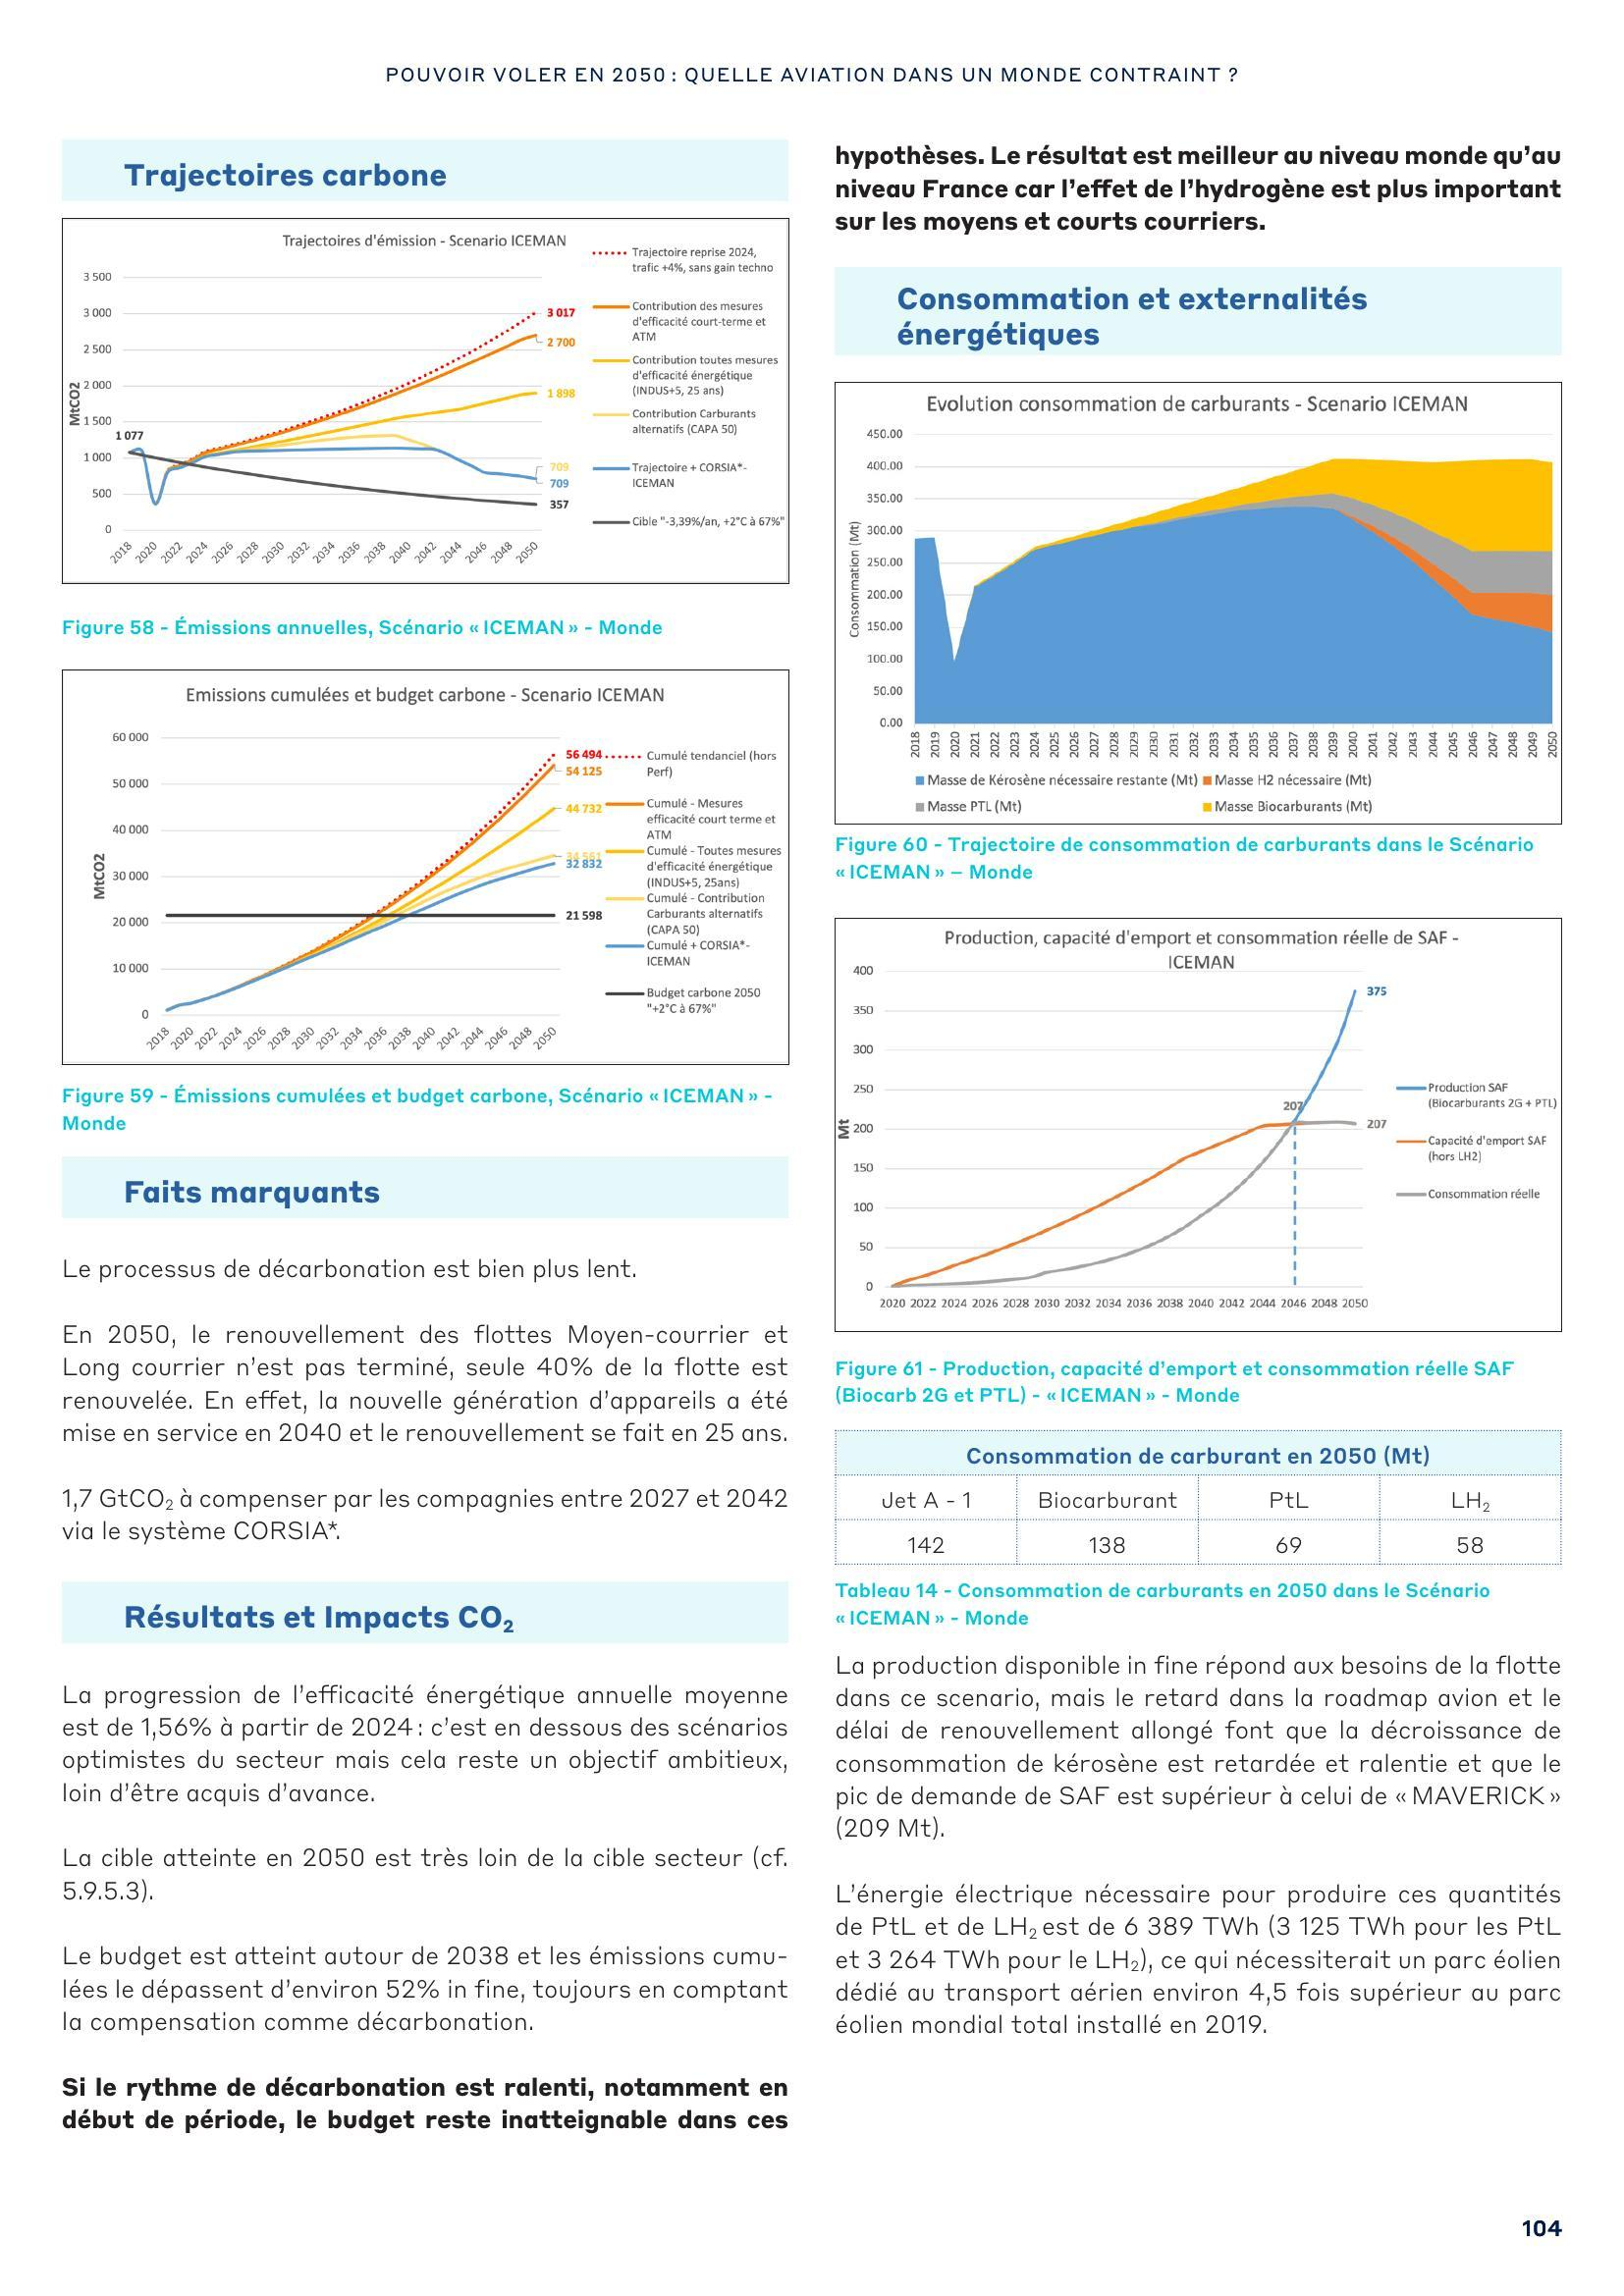
\includegraphics[width=\textwidth]{images/colpali_images/dataset_samples/shift_1.jpeg}
        \end{subfigure} \ 
        \begin{subfigure}[t]{0.30\textwidth}
            \caption*{\textbf{Query}: Quelle partie de la production pétrolière du Kazakhstan provient de champs en mer ?}
            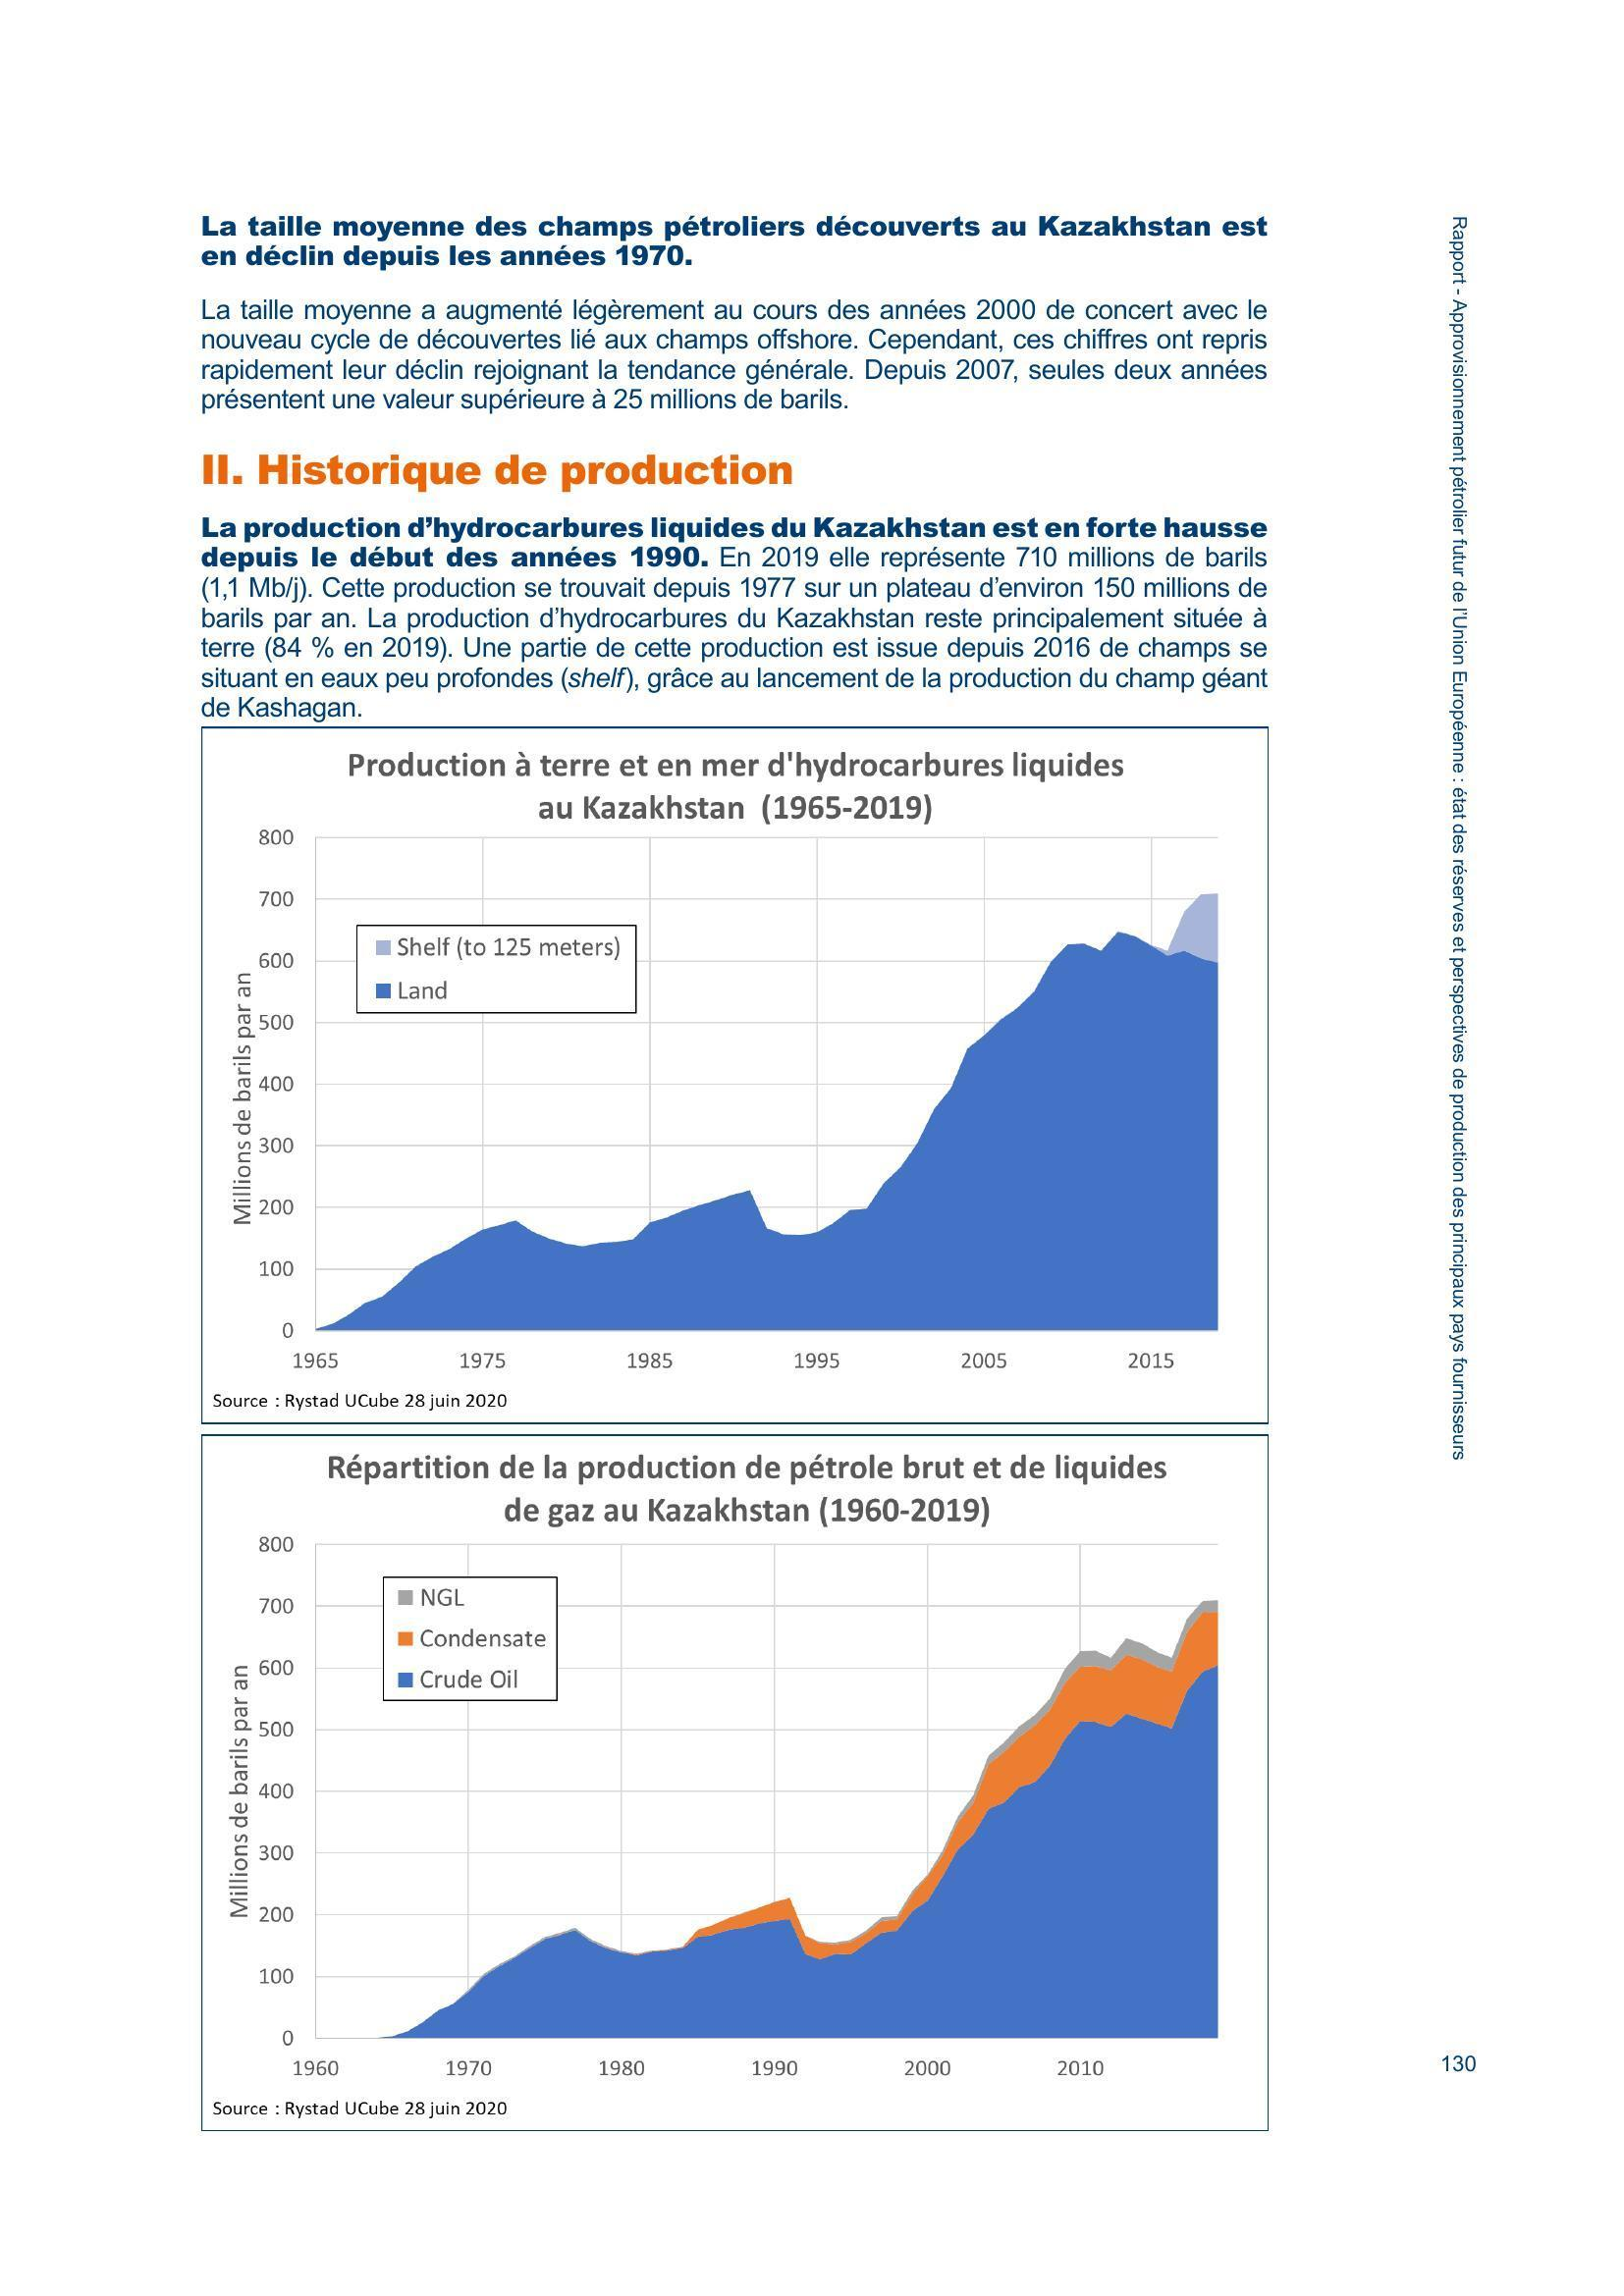
\includegraphics[width=\textwidth]{images/colpali_images/dataset_samples/shift_2.jpeg}
        \end{subfigure} \ 
        \begin{subfigure}[t]{0.30\textwidth}
            \caption*{\textbf{Query}: Quels sont les pays ayant la plus grande part des découvertes cumulées de pétrole brut en 2020 (en milliers de barils, hors découvertes cumulées) ?}
            \includegraphics*[width=\textwidth]{images/colpali_images/dataset_samples/shift_3.jpeg}
        \end{subfigure}modelsmodels
    \end{figure}

\end{center}

% \chapter{ViDoRe v3 Appendix}


\section{Dataset examples}

\begin{figure*}[h]
    \centering
    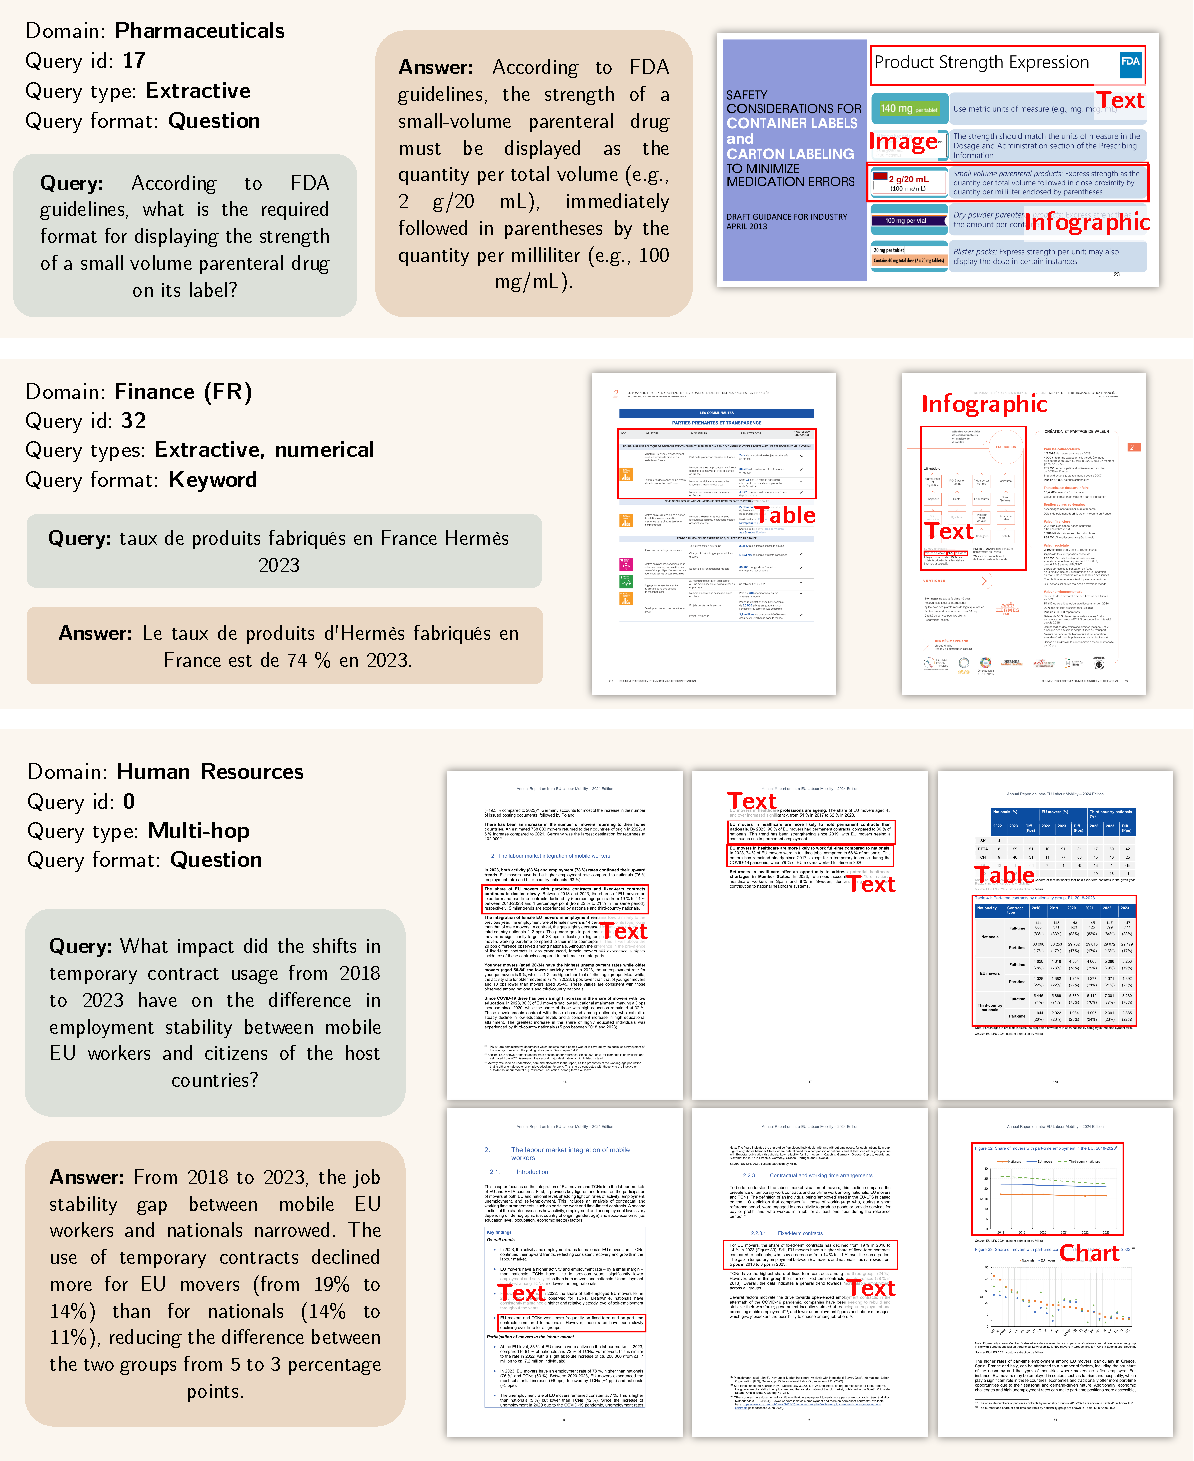
\includegraphics[width=0.92\textwidth]{images/vidorev3_images/dataset-examples.pdf}
    \caption{\textbf{Examples from the ViDoRe V3 datasets.} Featuring varied query types and visually rich document formats across multiple domains, the benchmark captures the complexity of real-world retrieval scenarios.}
\end{figure*}


\section{Supplementary benchmark details}

\paragraph{Domains} \Cref{tab:datasets} details the type of documents used in each corpus as well as several statistics.

\paragraph{Query type and format descriptions}

\Cref{tab:query_taxonomy} describes the types and formats of the queries, while \Cref{fig:upset plot} gives details about query type intersection frequency.

\paragraph{Query type by generation method}

Query type distributions by generation method (Figure~\ref{fig:query type by generation method}) confirm that open-ended queries dominate synthetic queries as the synthetic pipeline attributed more weight to this type, while extractive queries dominate human-image queries since they are more naturally chosen by annotators.

\section{Annotator pool and training details}
\label{appendix: annotator pool}
\paragraph{Annotator Pool and Selection.} Annotation was conducted by a curated pool of 76 annotators who were selected based on having: (1) a bachelor's degree or higher in the relevant domain, (2) professional experience in the domain, (3) native-level language proficiency as required by task, and (4) prior experience with RAG, retrieval, or VQA annotation projects. Quality control was performed by 13 senior annotators with enhanced domain knowledge and extensive annotation experience, with project oversight provided by data leads with multiple years of experience in human data generation.

\paragraph{Training and Pilot Phase.} The annotation process began with a comprehensive onboarding phase where annotators received task-specific training using gold-standard examples. For each domain, a pilot of several hundred tasks was conducted with 100\% quality control coverage and multiple annotators per task. During this phase, data leads and the research team continuously evaluated annotations, provided clarifications, and refined guidelines. Inter-annotator agreement and time-per-task baselines were calculated to establish ongoing evaluation benchmarks. The pilot concluded upon validation of both data quality and guideline effectiveness.

\section{Supplementary agreement metrics}
\label{appendix: relevance agreement}

Pages were pre-filtered by a VLM before human annotation; as most pages shown to annotators were likely relevant, this created a skewed class distribution. This prevalence imbalance causes traditional chance-corrected metrics like Krippendorff's Alpha to appear paradoxically low even when annotators genuinely agree, as inflated expected chance agreement penalizes the score. To address this, we report 2 complementary metrics: Krippendorff's Alpha (ordinal) as the standard measure and Gwet's AC2 which remains stable under prevalence skew. Overall, annotators achieved $\alpha = 0.469$, AC2 $= 0.760$. The divergence between Alpha and AC2/Weighted Agreement is expected given the pre-filtered data and confirms substantial agreement despite the skewed distribution.

\section{Supplementary retrieval details}
\label{appendix:supp retrieval}
\paragraph{Retriever model reference}

Table~\ref{tab:model_metadata} lists the retriever models evaluated in this work, along with their HuggingFace model names and citations.


\paragraph{Monolingual performance} \label{sec:english retrievers}

Tables~\ref{tab: english-only retrieval} and \ref{tab: french-only retrieval} present the monolingual performance of our models, where retrieval is conducted using language-matched queries and documents for English and French, respectively.

\begin{table*}[t!]
\centering
\small % Options: \small, \footnotesize (smaller), or \scriptsize (smallest)
\begin{tabularx}{\textwidth}{lXX} % 'l' for auto-width category, 'X' for wrapping columns
\toprule
\textbf{Category} & \textbf{Definition} & \textbf{Example} \\ \midrule
\multicolumn{3}{c}{\textit{\textbf{Query Types}}} \\ \midrule
\textbf{Open-ended} & Seeks explanatory or descriptive information that requires synthesis. & What drives the rise in women's workforce involvement in EU nations? \\
\textbf{Extractive} & Requires the retrieval of a specific piece of information. & Bank of America preferred stock MM dividend rate \\
\textbf{Compare Contrast} & Mandates a comparison between multiple entities or data points. & Explain the factors contributing to the reduction in R2R rates for ANDAs. \\
\textbf{Boolean} & Poses a yes/no question necessitating multi-step reasoning. & Did JPMorganChase execute more than half of its planned repurchase program? \\
\textbf{Numerical} & Asks for a specific quantitative value that must be derived or calculated. & percentage increase in Morgan Stanley revenue from 2023 to 2024 \\
\textbf{Multi-hop} & Requires integrating information from multiple sections or sources. & Summarize the steps involved in error reporting in ISMP's MERP. \\
\textbf{Enumerative} & Requests a list of all instances sharing a common property. & Specify the ISCO codes used to define domestic workers in the EU. \\ \midrule
\multicolumn{3}{c}{\textit{\textbf{Query Formats}}} \\ \midrule
\textbf{Question} & An interrogative sentence. & What was Citigroup's net interest margin in 2024? \\
\textbf{Keyword} & A non-verbal phrase or set of terms. & female employment rate European Union 2023 \\
\textbf{Instruction} & A directive specifying a task. & Identify the use case of a drill point gauge. \\ \bottomrule
\end{tabularx}
\caption{Taxonomy of Query Types and Formats.}
\label{tab:query_taxonomy}
\end{table*}

% \vspace{15cm}
% \hfill

\begin{figure*}[t!]
    \centering
    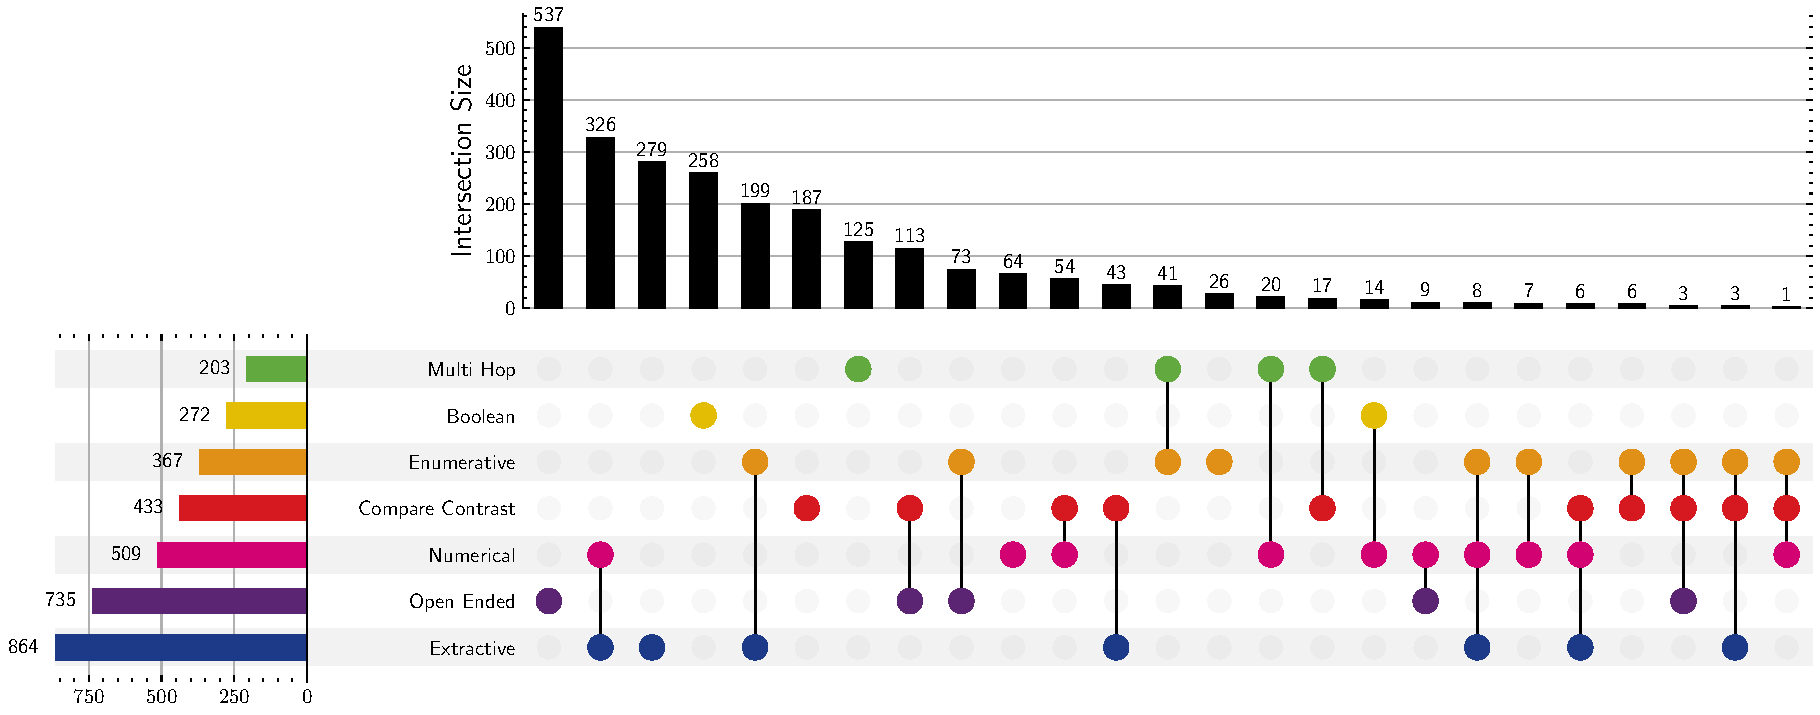
\includegraphics[width=\textwidth]{images/vidorev3_images/upset_plot_query_types_complete.pdf}
    \caption{\textbf{UpSet plot illustrating the distribution and intersection of query types in ViDoRe V3.} The horizontal bars on the left display the total count of queries for each individual type. The vertical bars at the top represent the frequency of specific combinations (intersections), as indicated by the connected dots in the matrix below. While \textit{Extractive} queries are the most prevalent overall, \textit{Open Ended} queries form the dominant unique category. Complex dependencies are evident in the frequent intersection of \textit{Enumerative} and \textit{Extractive types}, indicating a substantial subset of queries requiring list-based fact retrieval.} 
    \label{fig:upset plot}
\end{figure*}

% \clearpage

\begin{table*}[t]
\small
\centering
\setlength{\tabcolsep}{4pt}
\renewcommand{\arraystretch}{1.15}

\begin{tabularx}{\textwidth}{
    >{\RaggedRight\arraybackslash}X
    >{\RaggedRight\arraybackslash}X
    >{\RaggedRight\arraybackslash}p{4.2cm}
    c
    c
    c
    c
    >{\RaggedRight\arraybackslash}X
}
\toprule
\textbf{Corpus} &
\textbf{Domain(s)} &
\textbf{Description} &
\textbf{Lang.} &
\textbf{\# Docs} &
\textbf{\# Pages} &
\textbf{\# Queries$^{*}$} &
\textbf{Main modalities} \\
\midrule

\textbf{U.S. Public Company Annual Reports} &
Finance-EN &
Consists of 6 10-K annual reports from major U.S. financial institutions for the fiscal year ended December 31, 2024. &
en & 6 & 2942 & 309 &
Text, Table \\
\addlinespace

\textbf{Computer Science Textbooks} &
Computer Science / Education &
Consists of two open-source, peer-reviewed textbooks from OpenStax covering foundational topics in computer science, Python, and data science. &
en & 2 & 1360 & 215 &
Books \\
\addlinespace

\textbf{FDA Reports} &
Pharmaceuticals &
Consists of FDA presentations and Springer books (2016--2023) covering regulatory policies, drug development, and public health initiatives. &
en & 52 & 2313 & 364 &
Slides, Books \\
\addlinespace

\textbf{HR Reports from EU} &
HR &
Includes recent European Commission reports and papers on EU labour markets, social development, and employment policies. &
en & 14 & 1110 & 318 &
Reports \\
\addlinespace

\textbf{USAF Technical Orders} &
Industrial Maintenance &
Comprises U.S. military technical orders and manuals for aircraft maintenance, safety procedures, and material handling, revised through 2025. &
en & 27 & 5244 & 283 &
Manuals \\
\addlinespace

\textbf{French Physics Lectures} &
Physics &
A collection of educational materials offering an interdisciplinary exploration of modern physics and complexity science. &
fr & 42 & 1674 & 302 &
Slides \\
\addlinespace

\textbf{French Public Company Annual Reports} &
Finance-FR &
Contains the 2023--2024 annual reports of major French luxury companies (Dior, Hermès, Kering, L'Oréal, LVMH). &
fr & 5 & 2384 & 320 &
Reports \\
\addlinespace

\textbf{French Governmental Energy Reports} &
Energy &
Gathers official documents from French public agencies on energy, economic, and environmental issues in France. &
fr & 42 & 2229 & 308 &
Reports, Slides \\
\bottomrule
\end{tabularx}

\caption{Description of ViDoRe V3 public corpora. $^{*}$Number of queries is without translations}
\label{tab:datasets}
\end{table*}

% \textbf{Nuclear} \newline \textbf{Power Plant} \newline \textbf{Docs} & 
    % Nuclear Energy & 
    % Contains regulatory documents from 2004-2006 concerning the Vermont Yankee Nuclear Power Station's proposed power uprate. &
    % en & 
    % 48 & 
    % 2814 & 
    
    % Reports, Email \\
    % \addlinespace


    % \textbf{Internet} \newline \textbf{Protocols} & 
    % Telecom & 
    % A collection of IETF RFCs and standards documents defining core internet protocols, network management, and communication standards. & 
    % en & 
    % 123 & 
    % 4627 & 
    %  & 
    % Reports \\
    % \addlinespace



% \clearpage


% \begin{figure*}[t!]
%     \centering
%     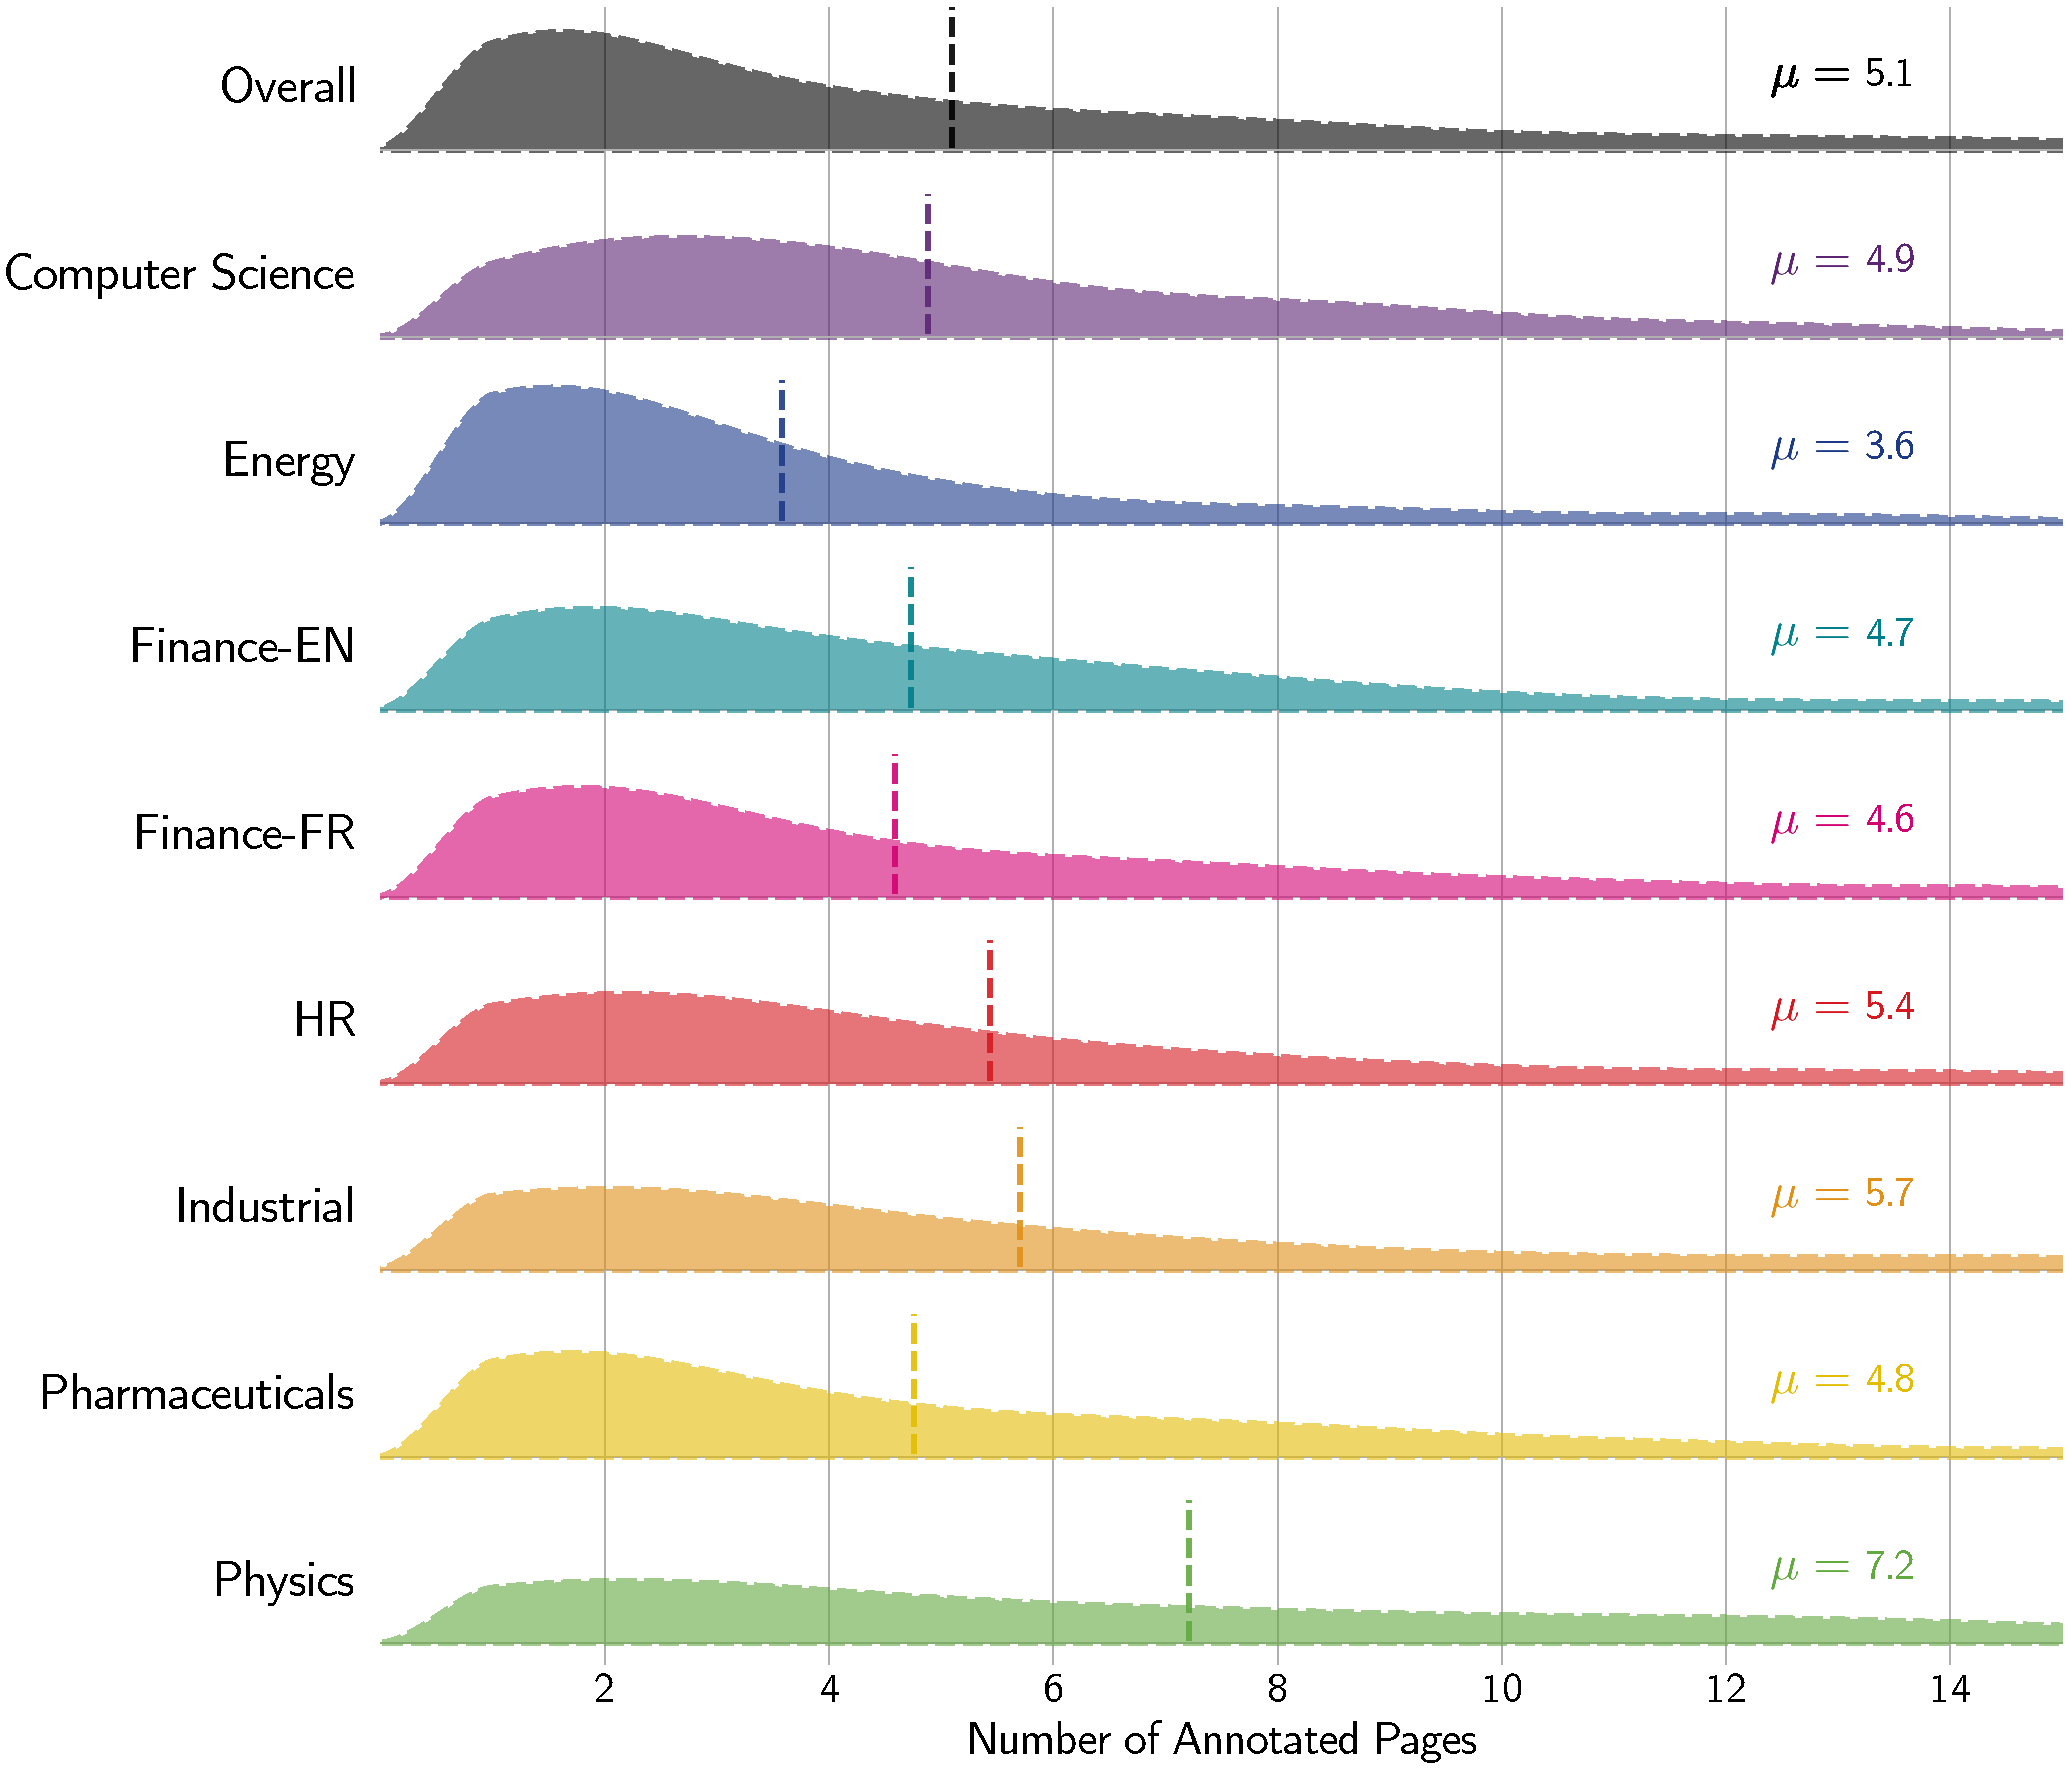
\includegraphics[clip, width=0.7\textwidth]{images/vidorev3_images/ridge_plot.pdf}
%     \caption{\textbf{Distribution of annotated page counts across domains.} This ridge plot displays the density of annotated pages per document for each specific domain, with vertical dashed lines marking the mean values. While the global average is $5.1$ pages, the distributions reveal distinct domain-specific characteristics: \textit{Physics} is a notable outlier, exhibiting the highest mean ($\mu=7.2$) and a heavy tail, suggesting that relevant information is often sparse and scattered across multiple pages. In contrast, \textit{Energy} queries appear more localized ($\mu=3.6$), with evidence typically concentrated within a narrower range.}
%     \label{fig:ridge_plot_query_types}
% \end{figure*}



\begin{figure*}[t!]
    \centering
    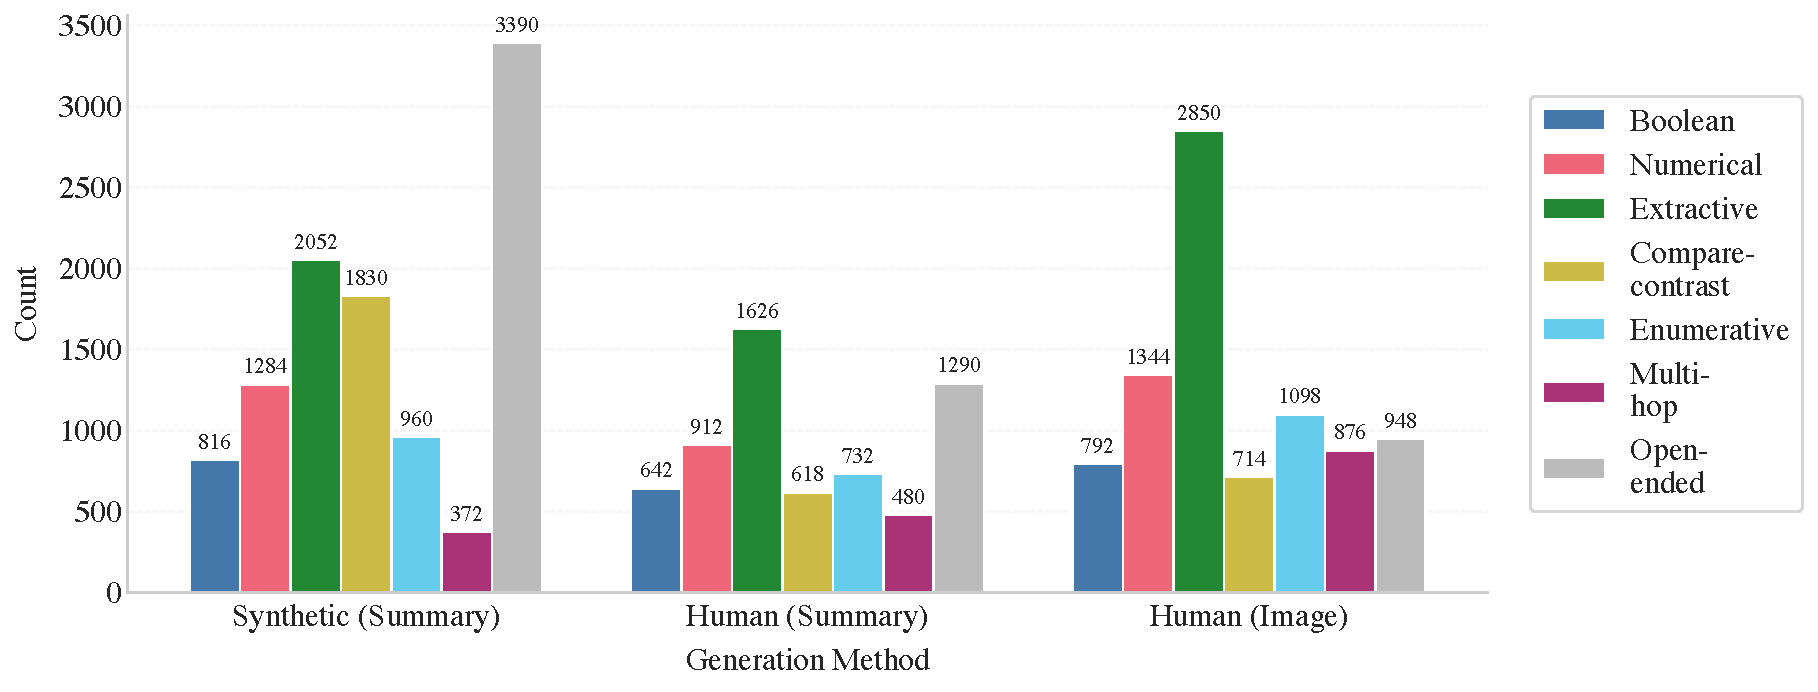
\includegraphics[clip, width=\textwidth]{images/vidorev3_images/query_types_by_generation_method.pdf}
    \caption{\textbf{Query type distribution by generation method.}}
    \label{fig:query type by generation method}
\end{figure*}

% \clearpage
% \paragraph{Page relevance scale}

% Table~\ref{tab:relevance_scale} details the relevance score rubrics provided to human annotator. Pages given a score of 0 were dropped from the final benchmark.

% \begin{table}[h]
% \small
% \centering
% \begin{tabular}{cXX}
% \toprule
% \textbf{Score} & \textbf{Label} & \textbf{Definition} \\
% \midrule
% 2 & Fully Relevant & The page contains the complete answer \\
% 1 & Critically Relevant & The page contains facts or information required to answer the query, though additional information is required \\
% 0 & Not Relevant & Provides no information relevant to the query \\
% \bottomrule
% \end{tabular}
% \caption{\textbf{Relevance scale used for page-level annotations.}}
% \label{tab:relevance_scale}
% \end{table}



%\paragraph{Ethics approval} 
%The annotation protocol was reviewed and approved by an ethics committee prior to the commencement of data collection. The review encompassed annotator recruitment procedures, compensation practices, task design, and data governance policies. Specific attention was given to ensuring that pay exceeded local minimum wage standards and that annotators were not exposed to harmful content. %\anto{Made up paragraph, we have to check with NVIDIA}


\begin{table}[H]
\centering

\resizebox{\columnwidth}{!}{%
\begin{tabular}{lccc}
\toprule
\textbf{Dataset} & \textbf{$\alpha$ (ord)} & \textbf{Gwet's AC2} \\ %& \textbf{Wgt. Agree} \\
\midrule
Computer science& 0.467 & 0.809 \\%& 0.849 \\
Energy & 0.463 & 0.714 \\%& 0.805 \\
Finance (EN) & 0.514 & 0.798 \\%& 0.832 \\
Finance (FR) & 0.320 & 0.736 \\%& 0.801 \\
H.R. & 0.413 & 0.793 \\%& 0.840 \\
Industrial Maintenance & 0.496 & 0.740 \\%& 0.803 \\
Telecom & 0.464 & 0.772 \\%& 0.833 \\
Nuclear & 0.389 & 0.794 \\%& 0.837 \\
Pharma & 0.478 & 0.755 \\%& 0.831 \\
Physics & 0.213 & 0.334 \\%& 0.668 \\
\midrule
\textbf{Overall} & \textbf{0.469} & \textbf{0.760} \\%& \textbf{0.815} \\
\bottomrule
\end{tabular}
}
\caption{Inter-annotator agreement for relevance ratings by dataset.}
\label{tab:iaa}
\end{table}



\begin{table*}[ht]
% \small
\centering
\begin{tabular}{lll}
\toprule
\textbf{Model alias} & \textbf{Full model name} & \textbf{Reference} \\ \midrule
Qwen3-8B & Qwen3-Embedding-8B & \cite{qwen3embedding} \\
Jina-v4 & jina-embeddings-v4 & \cite{günther2025jinaembeddingsv4universalembeddingsmultimodal} \\
Qwen3-0.6B & Qwen3-Embedding-0.6B & \cite{qwen3embedding} \\
LFM2-350M & LFM2-ColBERT-350M & \cite{liquidai2025lfm2} \\
BGE-M3 & BGE-M3 & \cite{chen_bge_2024} \\
BM25S & BM25S & \cite{bm25s} \\
ColEmbed-3B-v2 & llama-nemoretriever-colembed-3b-v2 & \cite{xu2025llamanemoretrievercolembedtopperforming} \\ % asked Gabriel about this
ColNomic-7B & colnomic-embed-multimodal-7b & \cite{nomicembedmultimodal2025} \\
ColEmbed-3B & llama-nemoretriever-colembed-3b-v1 & \cite{xu2025llamanemoretrievercolembedtopperforming} \\
ColNomic-3B & colnomic-embed-multimodal-3b & \cite{nomicembedmultimodal2025} \\
ColEmbed-1B & llama-nemoretriever-colembed-1b-v1 & \cite{xu2025llamanemoretrievercolembedtopperforming} \\
ColQwen2.5 & colqwen2.5-v0.2 & \cite{faysse2025colpaliefficientdocumentretrieval} \\
Nomic-7B & nomic-embed-multimodal-7b & \cite{nomicembedmultimodal2025} \\
ColQwen2 & colqwen2-v1.0 & \cite{faysse2025colpaliefficientdocumentretrieval} \\
Nomic-3B & nomic-embed-multimodal-7b & \cite{nomicembedmultimodal2025} \\
ColPali & colpali-v1.3 & \cite{faysse2025colpaliefficientdocumentretrieval} \\
Mxbai Edge 32M & mxbai-edge-colbert-v0-32m & \cite{takehi2025fantasticsmallretrieverstrain} \\
GTE-ModernColBERT & GTE-ModernColBERT-v1 & \cite{GTE-ModernColBERT} \\
ColModernVBERT & colmodernvbert & \cite{teiletche2025modernvbert} \\
ColSmol-256M & colSmol-256M & \cite{marafioti2025smolvlmredefiningsmallefficient} \\
\bottomrule
\end{tabular}
\caption{\textbf{Retriever reference table.} Model aliases used in Tables~\ref{tab:retriever_comparison_updated},~\ref{tab: english-only retrieval}, and~\ref{tab: french-only retrieval} are mapped to their HuggingFace model name and citation.}
\label{tab:model_metadata}
\end{table*}

% \paragraph{Retrieval performance with model size}

% \vic{To fill}

% \begin{figure}[h!]
%     \centering
%     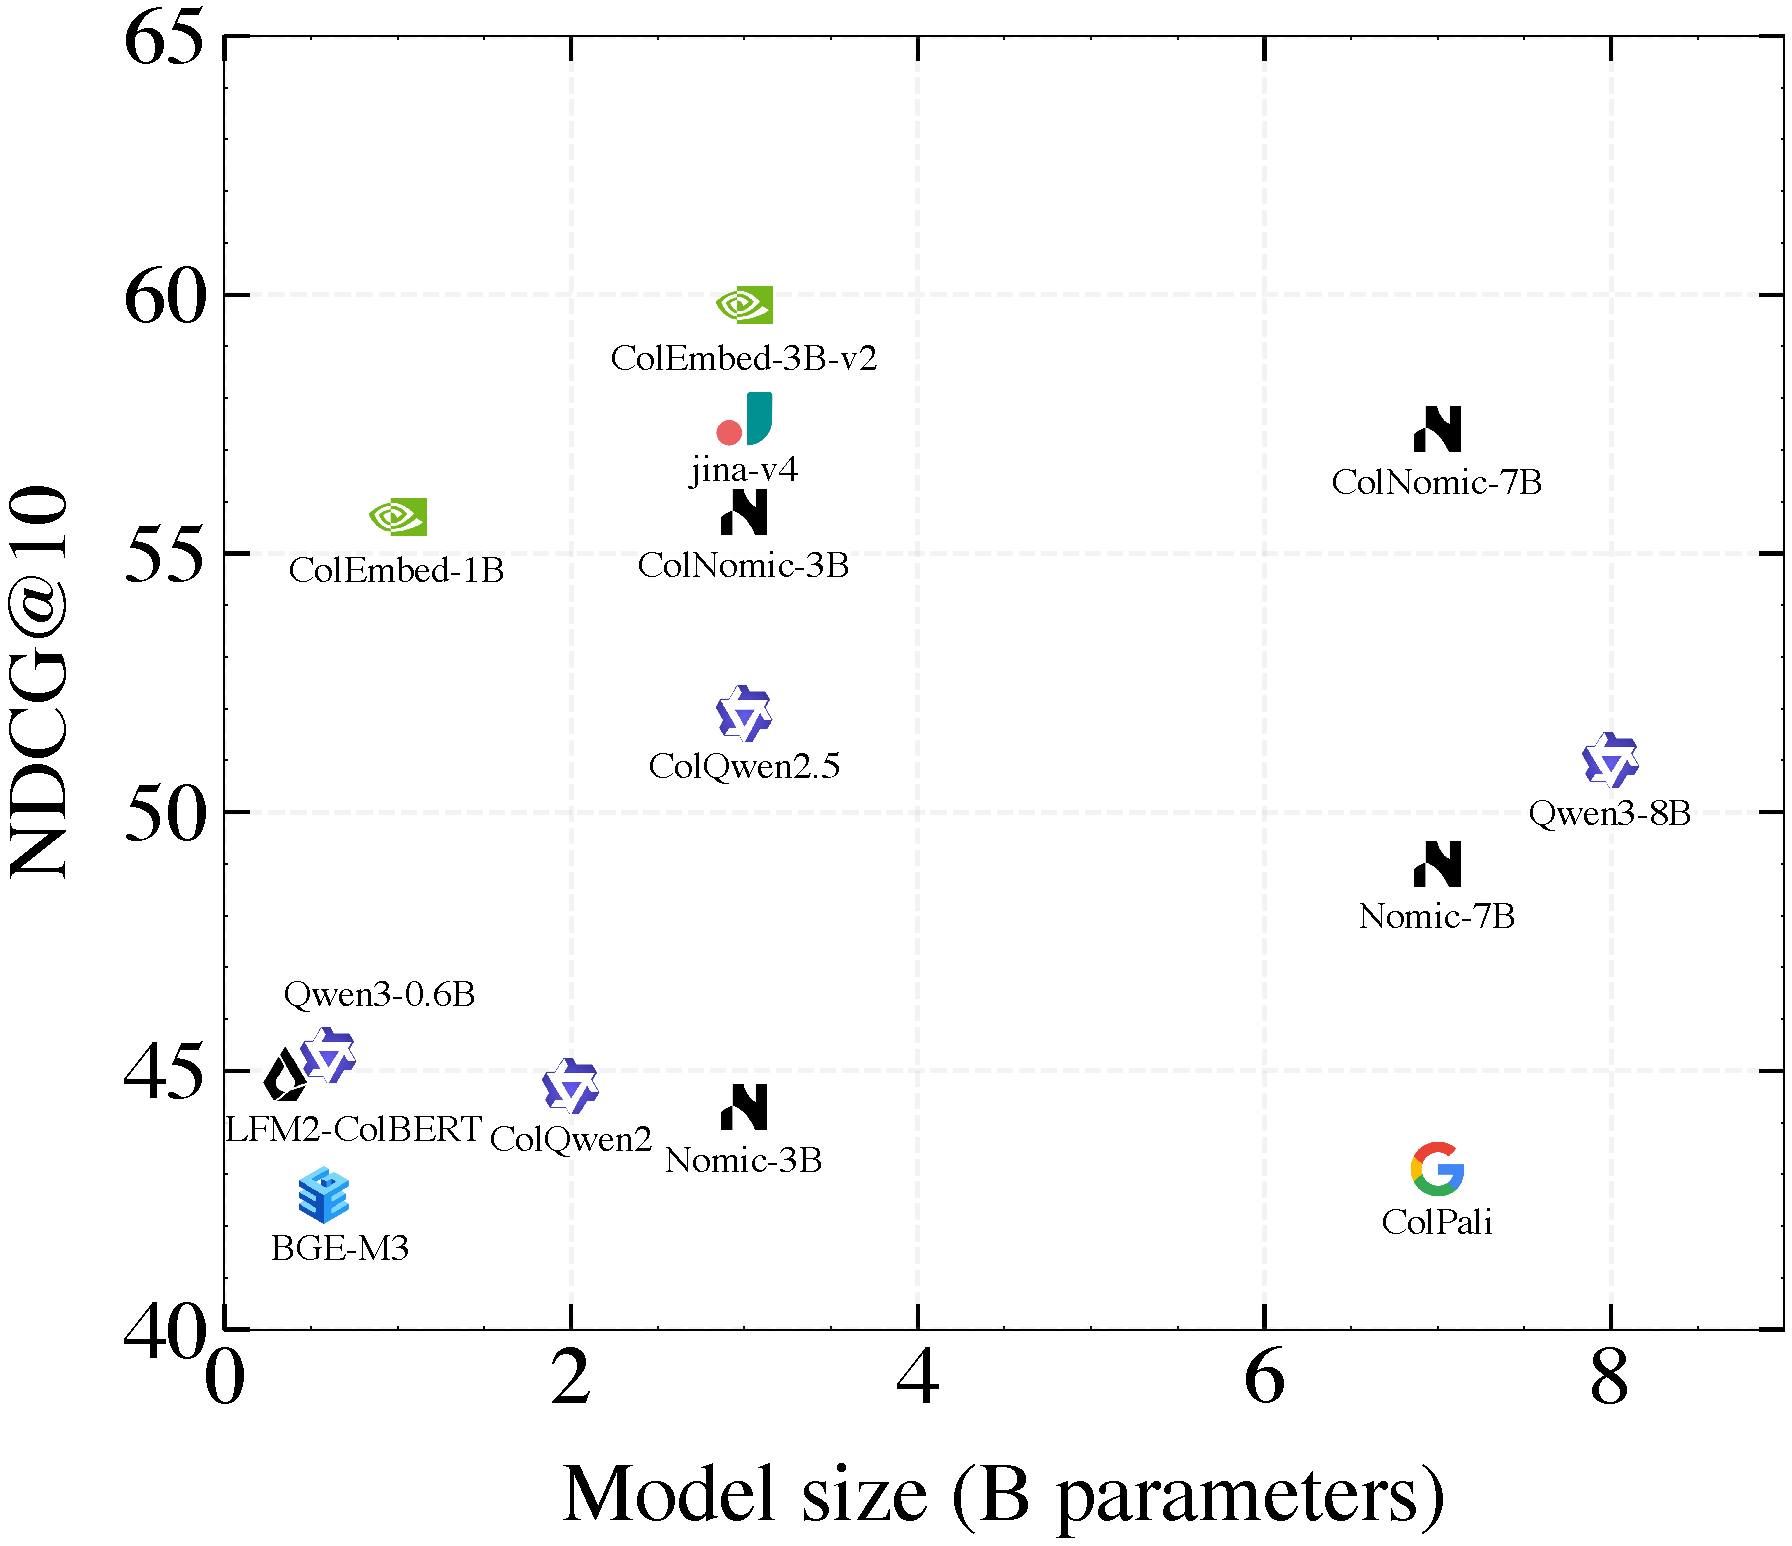
\includegraphics[width=\columnwidth]{images/vidorev3_images/size-performance_large_no_tomoro.pdf}
%     \caption{\textbf{Scaling of benchmark retrieval performance with model size.}} 
%     \label{fig:size-performance}
% \end{figure}


\begin{table*}[h!]
\centering
%\resizebox{\textwidth}{!}{%
\begin{tabular}{l c c c c c c c c >{\columncolor{avgcol}}c}
\toprule
\textbf{Model} & Size (B) & C.S. & Nucl. & Fin. & Phar. & H.R. & Ind. & Tele. & \textbf{Average} \\
\midrule
\multicolumn{9}{l}{\textit{\textbf{Textual Retrievers}}} \\
Jina-v4	& 3 & 67.3	& \textbf{48.2} & \textbf{56.5}&  59.0& \textbf{58.8} & 	45.8	& 61.0	& \textbf{56.7}\\
Qwen3-8B$^\bigstar$	& 8 & \textbf{73.5}	& 42.2	 & 54.8	& 62.4	& 52.3	& 45.3	& \textbf{66.0}	& 56.6 \\
LFM2-350M & 0.35 & 70.6 & 45.4 & 48.3 & 62.1 & 53.2 & \textbf{47.9} & 63.8 & 55.9\\
Mxbai Edge 32M & 0.03 & 68.0 & 44.4 & 48.2 & \textbf{62.5} & 52.7 & 47.1 & 61.9 & 55.0 \\
BM25S	& - & 64.7&	45.9&	49.9&	56.9&	49.6&	45.6	&58.3	&53.0\\
Qwen3-0.6B$^\bigstar$& 0.6 &	70.5	& 39.7	&51.5	& 57.4	& 46.2	&42.4	&59.7	&52.3\\
GTE-ModernColBERT & 0.15 & 63.6 & 41.7 & 39.8 & 62.0 & 46.2 & 44.6 & 59.7 & 51.1\\
BGE-M3$^\bigstar$	& 0.57 &63.6&	34.3	& 43.9	&54.7	&45.3	&39.0	&54.3	&47.9\\
\midrule
\multicolumn{9}{l}{\textit{\textbf{Visual Retrievers}}} \\
% tomoro-colqwen3-8b$^\blacktriangle$ & 77.6 & \textbf{53.7} & \textbf{70.8} & \textbf{68.1} & \textbf{66.8} & \textbf{58.9} & 70.8 & \textbf{66.7}\\
% tomoro-colqwen3-4b$^\blacktriangle$ & 78.0 & 52.3 & 69.7 & 67.8 & 64.1 & 58.8 & \textbf{72.5} & 66.2\\
ColEmbed-3B-v2 & 3 & \textbf{78.6} & 52.9 & 69.1 & \textbf{67.6} & \textbf{65.4} & 56.8 & \textbf{71.7} & \textbf{66.0} \\
ColEmbed-3B & 3 & 77.8 & \textbf{53.4} & \textbf{69.5 }& 66.9 & 64.9 & \textbf{57.0} & 69.4 & 65.6 \\
ColEmbed-1B & 1 & 75.5 & 52.2 & 67.0 & 66.2 & 64.5 & 56.1 & 68.7 & 64.3 \\
Jina-v4 & 3 & 74.2 & 52.4 & 66.1 & 65.2 & 64.6 & 55.9 & 68.7 & 63.9 \\
ColNomic-7B & 7 & 78.2 & 48.2 & 63.1 & 64.6 & 62.9 & 54.2 & 69.6 & 63.0 \\
ColNomic-3B & 3 & 75.5 & 45.5 & 63.0 & 63.7 & 62.6 & 52.8 & 68.6 & 61.7 \\
ColQwen2.5 & 3 & 75.2 & 42.9 & 61.2 & 60.9 & 59.2 & 49.4 & 65.3 & 59.2 \\
Nomic-7B$^\bigstar$ & 7 & 70.9 & 42.3 & 57.6 & 63.8 & 55.9 & 48.5 & 62.0 & 57.3 \\
ColQwen2 & 2 & 73.5 & 44.1 & 50.9 & 58.1 & 54.7 & 49.8 & 63.2 & 56.3 \\
ColPali & 7 & 72.5 & 38.1 & 43.3 & 57.7 & 53.3 & 47.0 & 59.2 & 53.0 \\
Nomic-3B$^\bigstar$ & 3 & 62.1 & 37.2 & 53.3 & 59.2 & 51.9 & 41.1 & 57.2 & 51.7 \\
ColModernVBERT & 0.25 & 59.7 & 42.0 & 50.4 & 56.6 & 47.0 & 43.9 & 55.2 & 50.7 \\
ColSmol-256M & 0.25 & 57.4 & 36.5 & 47.7 & 51.4 & 46.0 & 38.5 & 47.5 & 46.4 \\
\bottomrule
\end{tabular}
%}
\caption{\textbf{English-only retrieval performance (NDCG@10).} $\bigstar$: single-vector models. Results are computed on the English queries of the English datasets.}
\label{tab: english-only retrieval}
\end{table*}


\begin{table*}[h!]
\small
\centering
%\resizebox{\textwidth}{!}{%
\begin{tabular}{l c c c c >{\columncolor{avgcol}}c}
\toprule
\textbf{Model} & Size (B) & Phys. & Ener. & Fin. & \textbf{Average} \\
\midrule
\multicolumn{5}{l}{\textit{\textbf{Textual Retrievers}}} \\
Jina-v4	& 3 & 44.0	& \textbf{63.4}	& \textbf{44.8} & \textbf{50.7}\\
Qwen3-8B$^\bigstar$	& 8 &\textbf{45.8}	& 60.2	& 37.6& 47.9\\
Qwen3-0.6B$^\bigstar$	& 0.6 & 43.8	& 54.9	& 28.5& 42.4\\
BGE-M3$^\bigstar$ &0.57	& 38.3	& 53.1	& 28.4&39.9\\
BM25S	& - & 39.8	& 57.4	& 35.9 & 44.4\\
\midrule
\multicolumn{5}{l}{\textit{\textbf{Visual Retrievers}}} \\
ColEmbed-3B-v2 & 3 & 48.2 & 67.5 & 48.2 & \textbf{54.6}\\
ColNomic-7b	& 7 & \textbf{48.5} & 67.0	& 47.9 & 54.5\\
ColNomic-3b	& 3 & \textbf{48.5} &	\textbf{67.9} &	46.8 & 54.4\\
Jina-v4	& 3 & 46.8	& 66.7 & 48.6 & 54.0 \\
ColEmbed-3B & 	3 & 46.6 &	66.3 &	\textbf{48.9} & 53.9\\
ColEmbed-1B & 1 & 44.7 &	64.6 &	47.8 & 52.4\\
ColQwen2.5 &	3 & 47.8	&62.3	&43.6& 51.2\\
Nomic-7B$^\bigstar$ &	7 & 45.6&	61.6&	41.3 & 49.5\\
ColQwen2	& 3 & 43.9	&55.6	&26.5& 42.0\\
Nomic-3B$^\bigstar$	& 3 & 43.6	&56.4	&34.4 & 44.8\\
ColPali	& 7 & 43.2	&50.5	&23.6 & 39.1 \\
%ColModernVBERT	&27.9&	44.2&	27.0 & 33.0 \\
%ColSmol-256M	&19.1	&31.9	&20.8 & 23.9 \\
\bottomrule
\end{tabular}
%}
\caption{\textbf{French-only retrieval performance (NDCG@10).} $\bigstar$: single-vector models. Results are computed on the French queries of the French datasets.}
\label{tab: french-only retrieval}
\end{table*}

% \clearpage

\paragraph{Additional Retrieval Modality Performances} To evaluate the hybrid retrieval setup, we use the multimodal Jina-v4 model to generate separate visual and textual rankings. We then construct a hybrid retrieval set by merging the top-5 results from each modality and removing duplicates. Because this set-union operation does not preserve a strict ranking order, we report the unranked F1 score. As shown in \Cref{tab:hybrid_comparison}, the hybrid approach consistently outperforms single-modality baselines.

% \clearpage


\begin{table*}[t!]
\centering
% \resizebox{\columnwidth}{!}{%
\small
\begin{tabular}{l c c c c c c c c c c >{\columncolor{avgcol}}c}
\toprule
 & \multicolumn{7}{c}{\textbf{English Datasets}} & \multicolumn{3}{c}{\textbf{French Datasets}} & \multicolumn{1}{c}{} \\
\cmidrule(lr){2-8} \cmidrule(lr){9-11}
\textbf{Modality} & \shortstack{C.S.} & \shortstack{Nucl.} & \shortstack{Fin.} & \shortstack{Phar.} & \shortstack{H.R.} & \shortstack{Ind.} & \shortstack{Tel.} & \shortstack{Phys.} & \shortstack{Ener.} & \shortstack{Fin.} & \textbf{Avg.} \\
\midrule
Visual	& 39.4	& 25.5	& 28.4	& 27.5	& 30.0	& 21.4	& 31.4	&\textbf{26.6}	& 25.2	& 22.9	& 27.8 \\
Textual	& 35.4	& 23.1&	24.5	&24.2	&27.4&	16.5&	29.0&	25.8 &	23.9	&20.4&	25.0 \\
Hybrid	&\textbf{43.0}	&\textbf{27.7}	&\textbf{30.9}	&\textbf{29.7}	&\textbf{32.6}	&\textbf{22.2}	&\textbf{35.5}&	26.5	&\textbf{29.8}	&\textbf{24.3}	&\textbf{30.2} \\
\midrule
\textit{Avg. \# Pages for hybrid}	&\textit{6.96}	& \textit{7.38}	&\textit{7.77}&\textit{7.40}&	\textit{7.29}&	\textit{7.77}	&\textit{7.09} &	\textit{7.26}&	\textit{6.97}	&\textit{7.61}&	\textit{7.35} \\
\bottomrule
\end{tabular}
% }
\caption{\textbf{Performance comparison of retrieval modalities (F1@10) on Jina-v4.} Evaluation is performed using the multimodal retriever Jina-v4. The Hybrid method combines the top-5 visual and top-5 textual matches, subsequently removing duplicates. The final row reports the average number of unique pages remaining in the hybrid set. The Hybrid setup constantly outperforms both textual and visual retrieval.}
\label{tab:hybrid_comparison}
\end{table*}


% \clearpage

% \newpage


\section{ColEmbed-3B-v2 performance breakdown}\label{appendix: colembed-v2-perf-breakdown}

\Cref{tab:perf language} details the retrieval scores of ColEmbed-3B-v2 by query language, highlighting small performance variations by language.

% \begin{table}[h!]
% \centering
% \resizebox{\columnwidth}{!}{%
% \begin{tabular}{l ccc c}
% \toprule
% & \multicolumn{3}{c}{\textbf{Query Format}} & \\ % Labels the columns
% \cmidrule(lr){2-4}
% \textbf{Query Type} & Instruction & Keyword & Question & \textbf{Avg.} \\
% \midrule
% Boolean & — & — & 70.3 & 70.3 \\
% Numerical & 65.0 & 64.9 & 67.6 & 66.3 \\
% Extractive & 63.3 & 65.6 & 67.3 & 65.8 \\
% Compare-contrast & 59.3 & 59.2 & 61.3 & 60.0 \\
% Enumerative & 56.2 & 65.2 & 57.8 & 57.6 \\
% Multi-hop & 50.6 & — & 57.1 & 53.9 \\
% Open-ended & 48.0 & 45.8 & 50.6 & 48.6 \\
% \midrule
% \textbf{Avg.} & 55.6 & 56.4 & 62.6 & 59.5 \\
% \bottomrule
% \end{tabular}
% }
% \caption{\textbf{ColEmbed-3B-v2 NDCG@10 by query type and format.}}
% \label{tab:perf query type format}
% \end{table}

\paragraph{Performance by number of annotated pages}

As seen in Figure~\ref{fig:perf number of pages}, performance drops with the number of annotated pages. However, a potential confounding factor is the correlation between query type and the number of annotated pages, since more complex query types also have higher number of annotated pages (Figure~\ref{fig:num pages per query type}). We perform a stratified regression analysis to isolate these two effects.



We model NDCG@10 as a linear function of the number of annotated pages ($P$) stratified by query type. For each of the 7 query types, we fit an ordinary least squares regression:
\begin{equation*}
    NDCG@10 = a \cdot P + b + \epsilon.
\end{equation*}

Results in Figure~\ref{fig:perf content num pages} and Table~\ref{tab:num pages content type decay} reveal that all query types suffer a significant performance penalty as the number of annotated pages increases. Slope values are nearly uniform ($a \approx -0.024$), suggesting a similar drop in retrieval accuracy across most query types. The open-ended and enumerative types are the two exceptions: despite having the lowest NDCG@10 for low page counts, they also have the shallowest slope, which suggests that retrieval success on these queries is constrained by the model's fundamental difficulty in synthesizing multiple relevant sources rather than the volume of relevant context.

\begin{table}[!h]
\small
\centering
%\resizebox{\columnwidth}{!}{%
\begin{tabular}{lc}
\toprule
\textbf{Query Language} & \textbf{NDCG@10}\\
\midrule
English & 60.8 \\
French & 59.8 \\
Portuguese & 59.6 \\
Spanish & 59.6 \\
Italian & 59.1 \\
German & 57.9 \\
\bottomrule
\end{tabular}
%}
\caption{\textbf{ColEmbed-3B-v2 NDCG@10 by query language.}}
\label{tab:perf language}
\end{table}

\begin{figure}[t]
    \centering
    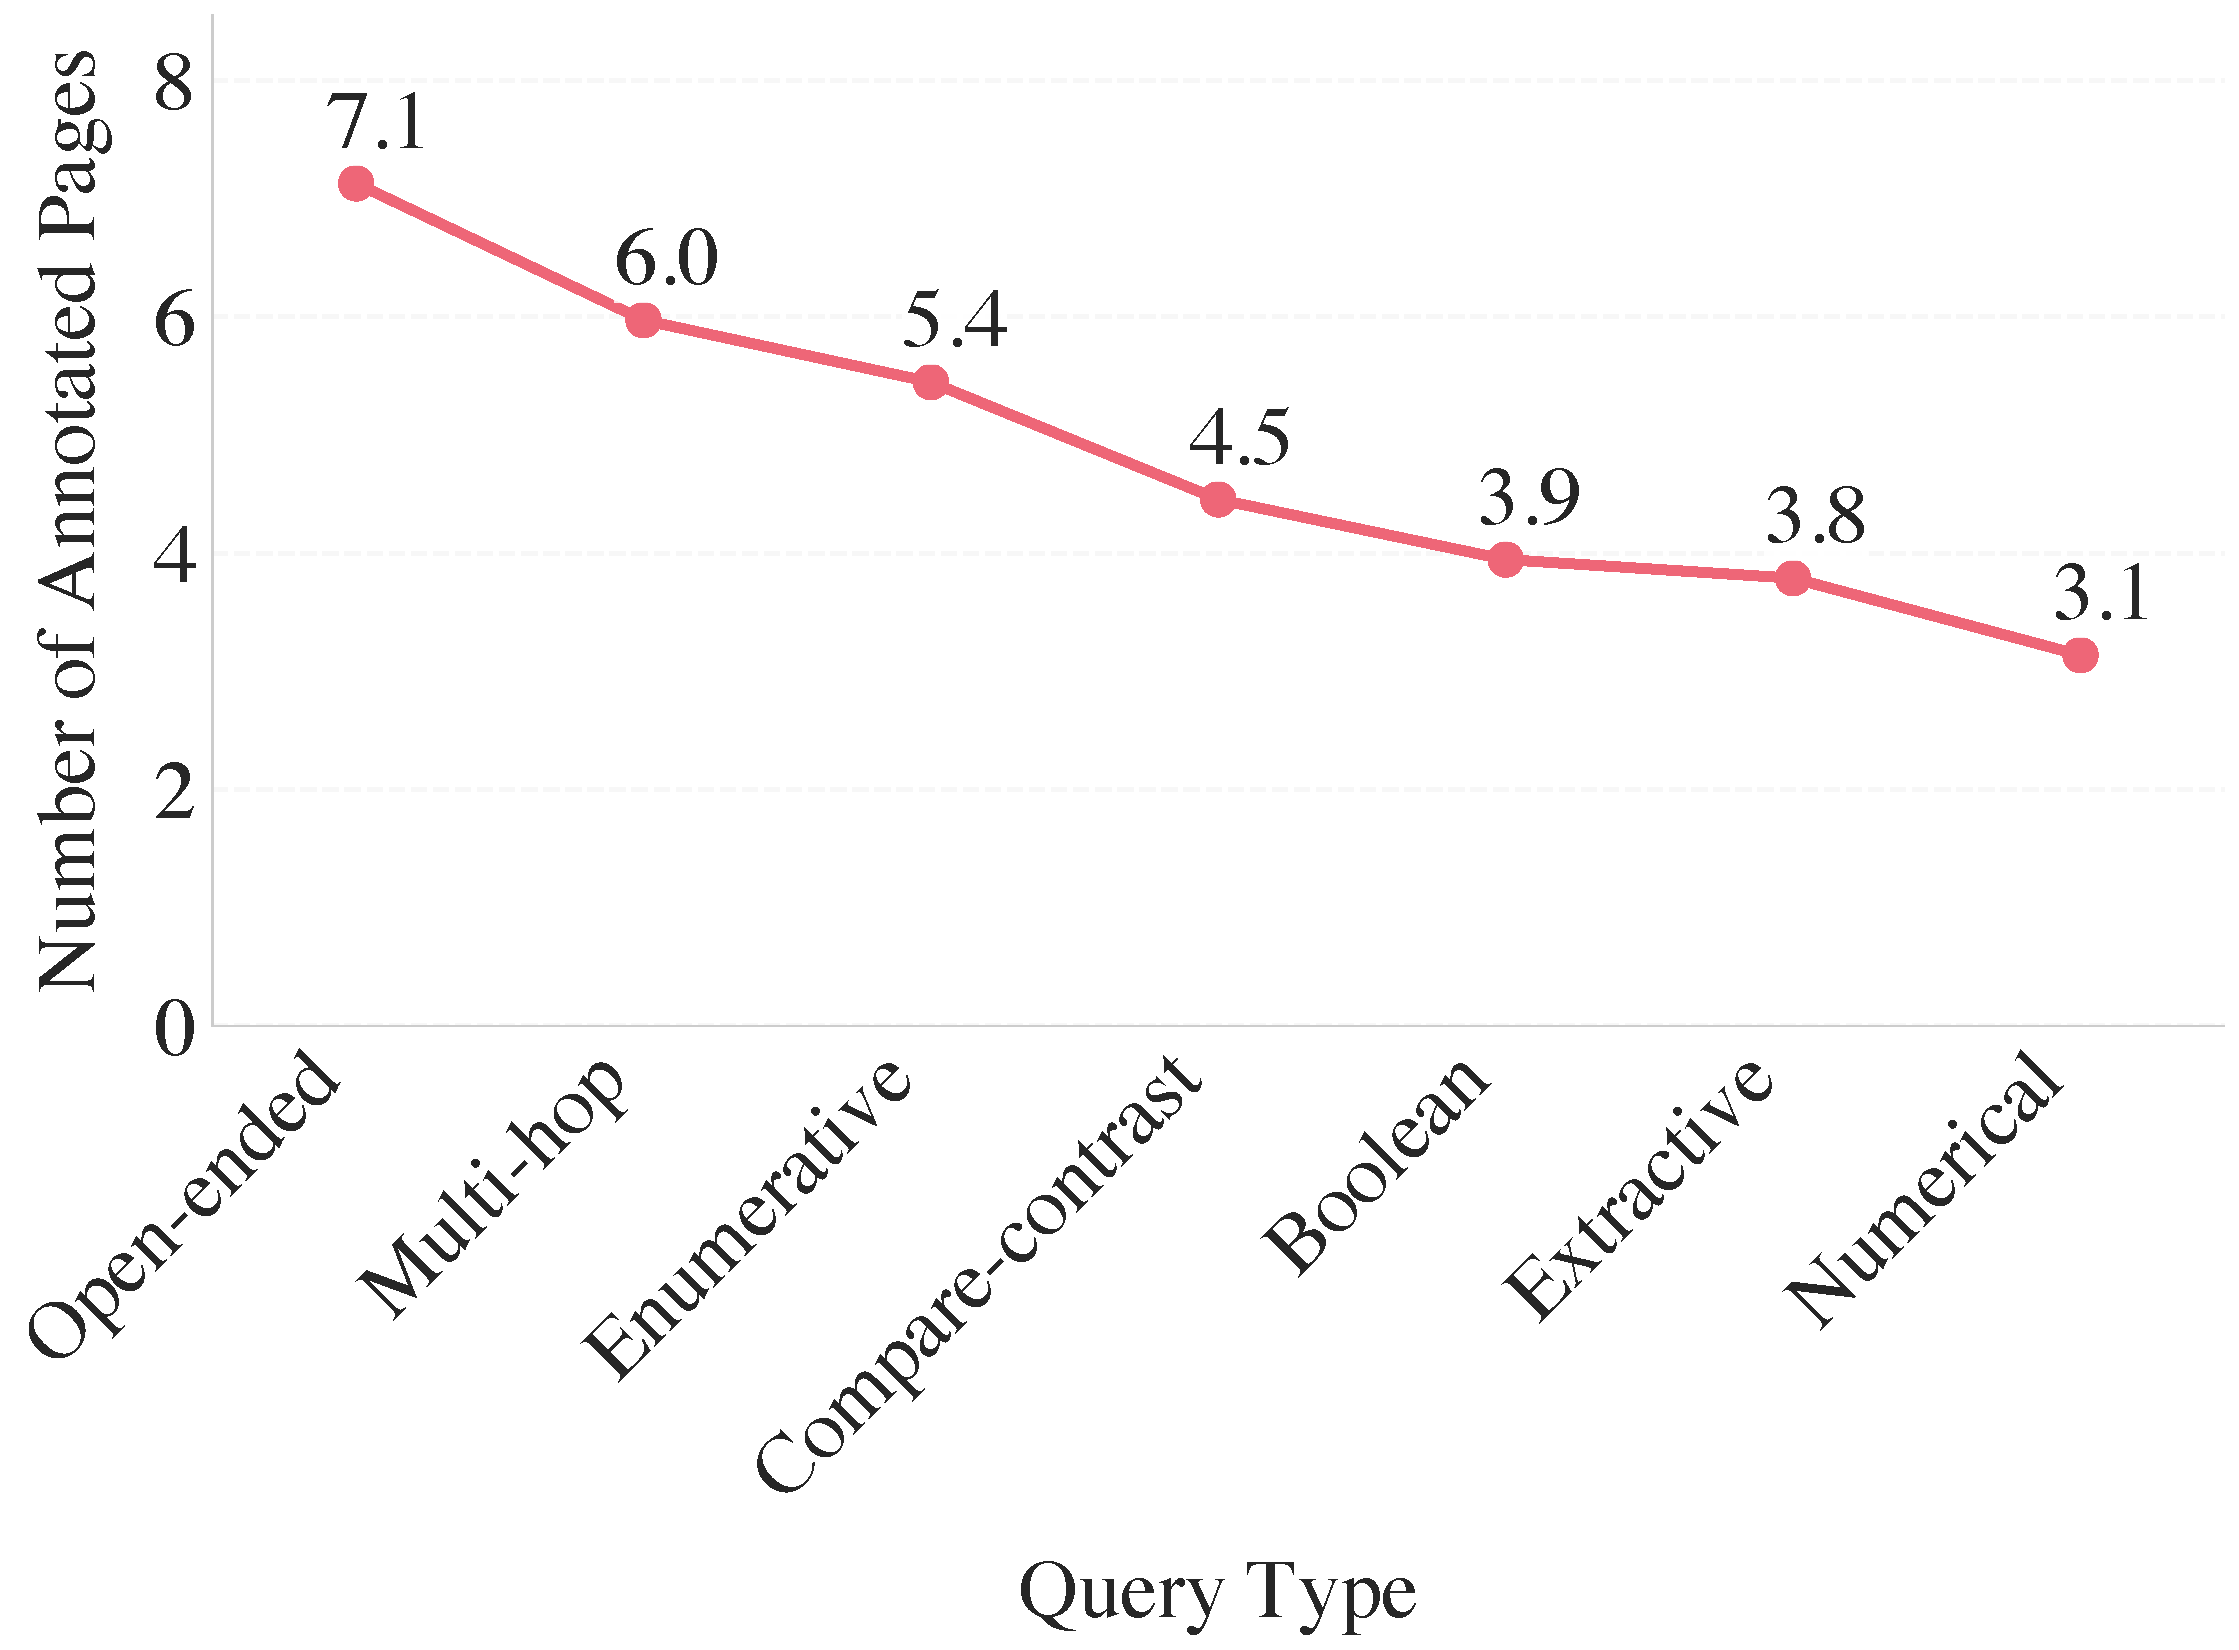
\includegraphics[width=0.9\columnwidth]{images/vidorev3_images/annotated_pages_by_query_type.pdf}
    \caption{\textbf{Average number of annotated pages by query type.}} 
    \label{fig:num pages per query type}
\end{figure}

\begin{figure}[h!]
    \centering
    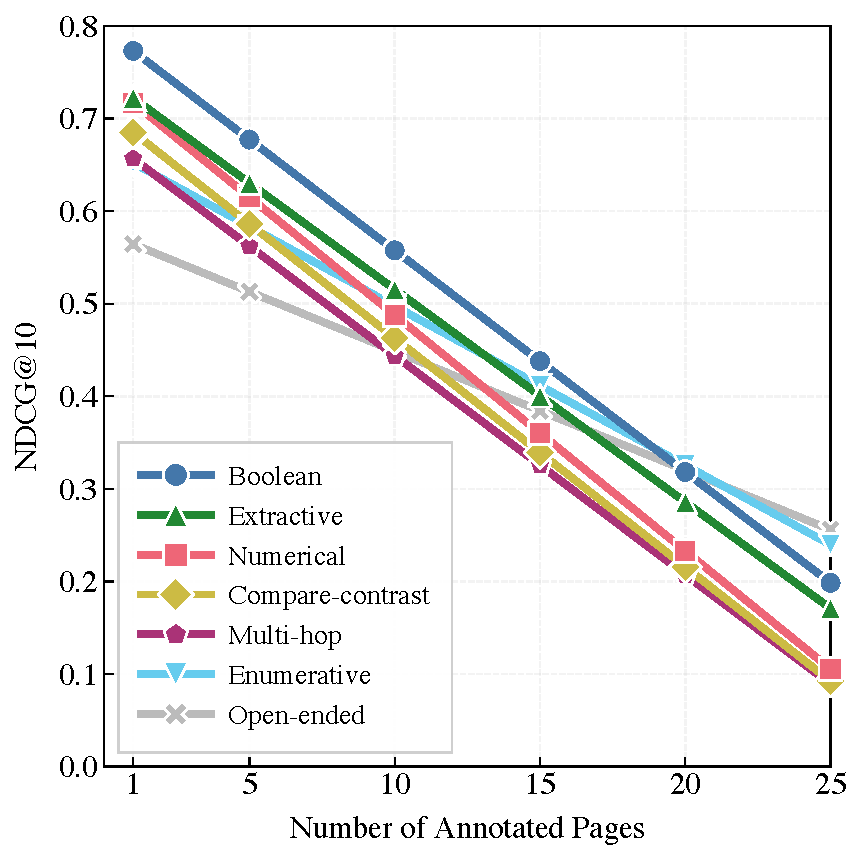
\includegraphics[width=0.8\columnwidth]{images/vidorev3_images/ndcg_query_type_num_pages.pdf}
    \caption{\textbf{ColEmbed-3B-v2 NDCG@10 by number of annotated pages and query type.}} 
    \label{fig:perf content num pages}
\end{figure}

\begin{table}[h!]
\centering
\small
\begin{tabular}{lccc}
\toprule
\textbf{Query Type} & Slope $a$ & Intercept $b$ & $R^2$ \\
\midrule
Boolean           & -0.0239 & 0.797 & 0.101 \\
Numerical         & -0.0255 & 0.742 & 0.059 \\
Extractive        & -0.0230 & 0.745 & 0.084 \\
Compare-contrast  & -0.0247 & 0.710 & 0.117 \\
Enumerative       & -0.0172 & 0.669 & 0.080 \\
Multi-hop         & -0.0237 & 0.680 & 0.114 \\
Open-ended        & -0.0129 & 0.577 & 0.057 \\
\bottomrule
\end{tabular}
\caption{\textbf{Linear regression analysis of NDCG@10 decay with number of annotated pages, by query type.} The slope $a$ represents performance sensitivity to retrieval context size, while the intercept $b$ represents intrinsic difficulty at minimum context size.}
\label{tab:num pages content type decay}
\end{table}

\paragraph{Performance by content type}

NDCG@10 by content type in Table~\ref{tab:perf content type} show that retrieval is more challenging for visual content, with Image performing 10pp below Text. However, content type and query type are correlated in our benchmark: for instance, tables appear in numerical queries 2.2 $\times$ more often than the baseline, while images are over-represented in open-ended queries (Figure~\ref{fig:lift content type}). Since numerical queries are easier than open-ended ones, we test whether the effect of content type is a byproduct of query type confounding. We fit an additive model that predicts performance as the sum of independent query-type and content-type effects. Figure~\ref{fig:ndcg content query residuals heatmap} shows the residuals which measure deviation from this baseline. We see that most residuals are below 5pp, indicating that the two factors combine additively without significant interaction.


\begin{table}[h!]
\small
\centering
%\resizebox{\columnwidth}{!}{%
\begin{tabular}{lcc}
\toprule
\textbf{Content type} & NDCG@10 & Content type count \\
\midrule
Text & 59.3 & 17244 \\
Chart & 56.3 & 2364 \\
Infographic & 55.2 & 2814 \\
Table & 53.9 & 6480 \\
Other & 50.8 & 492 \\
Image & 49.3 & 1140 \\
Mixed & 45.1 & 1164 \\
\bottomrule
\end{tabular}
%}
\caption{\textbf{ColEmbed-3B-v2 NDCG@10 by content type.} Content type is labeled on each annotated page based on the nature of the query-relevant content delimited by the bounding boxes. One page may be tagged with several content types if it contains multiple relevant sections of distinct nature. The Mixed type corresponds to annotations encompassing several content types.}
\label{tab:perf content type}
\end{table}

\begin{figure}[h!]
\centering
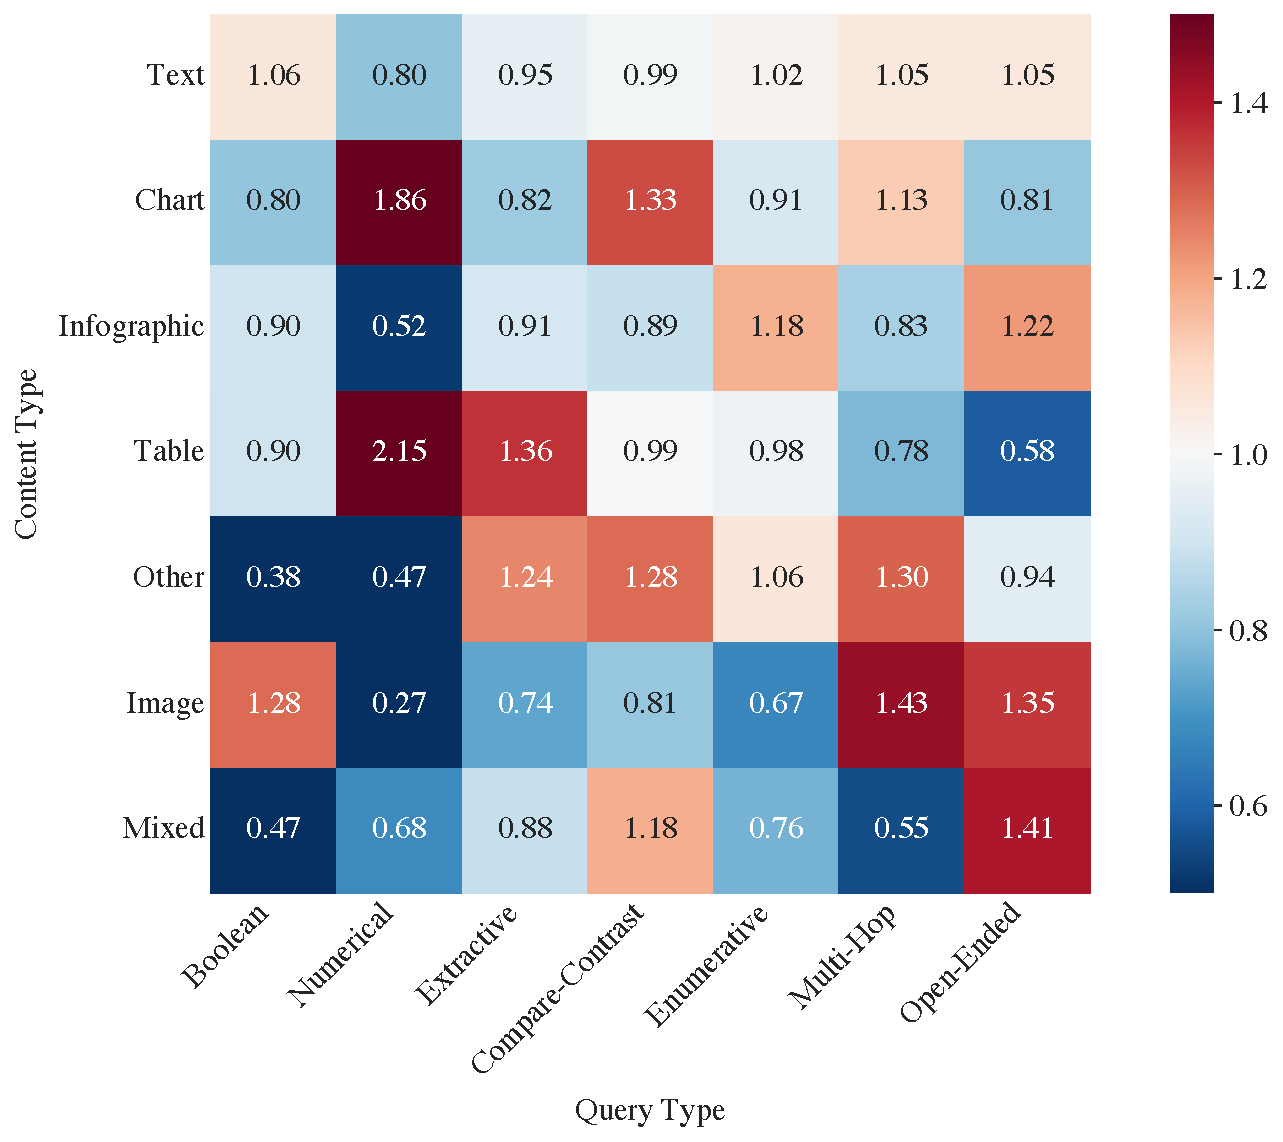
\includegraphics[width=\columnwidth]{images/vidorev3_images/lift_content_query_type.pdf}
\caption{\textbf{Lift of query types by content type.} Each cell shows the ratio of observed query type frequency to baseline frequency for a given content type. Values >1 indicate over-representation (e.g., tables appear 2.15× more in numerical queries than expected), while values <1 indicate under-representation.}
\label{fig:lift content type}
\end{figure}

\begin{figure}[h!]
\centering
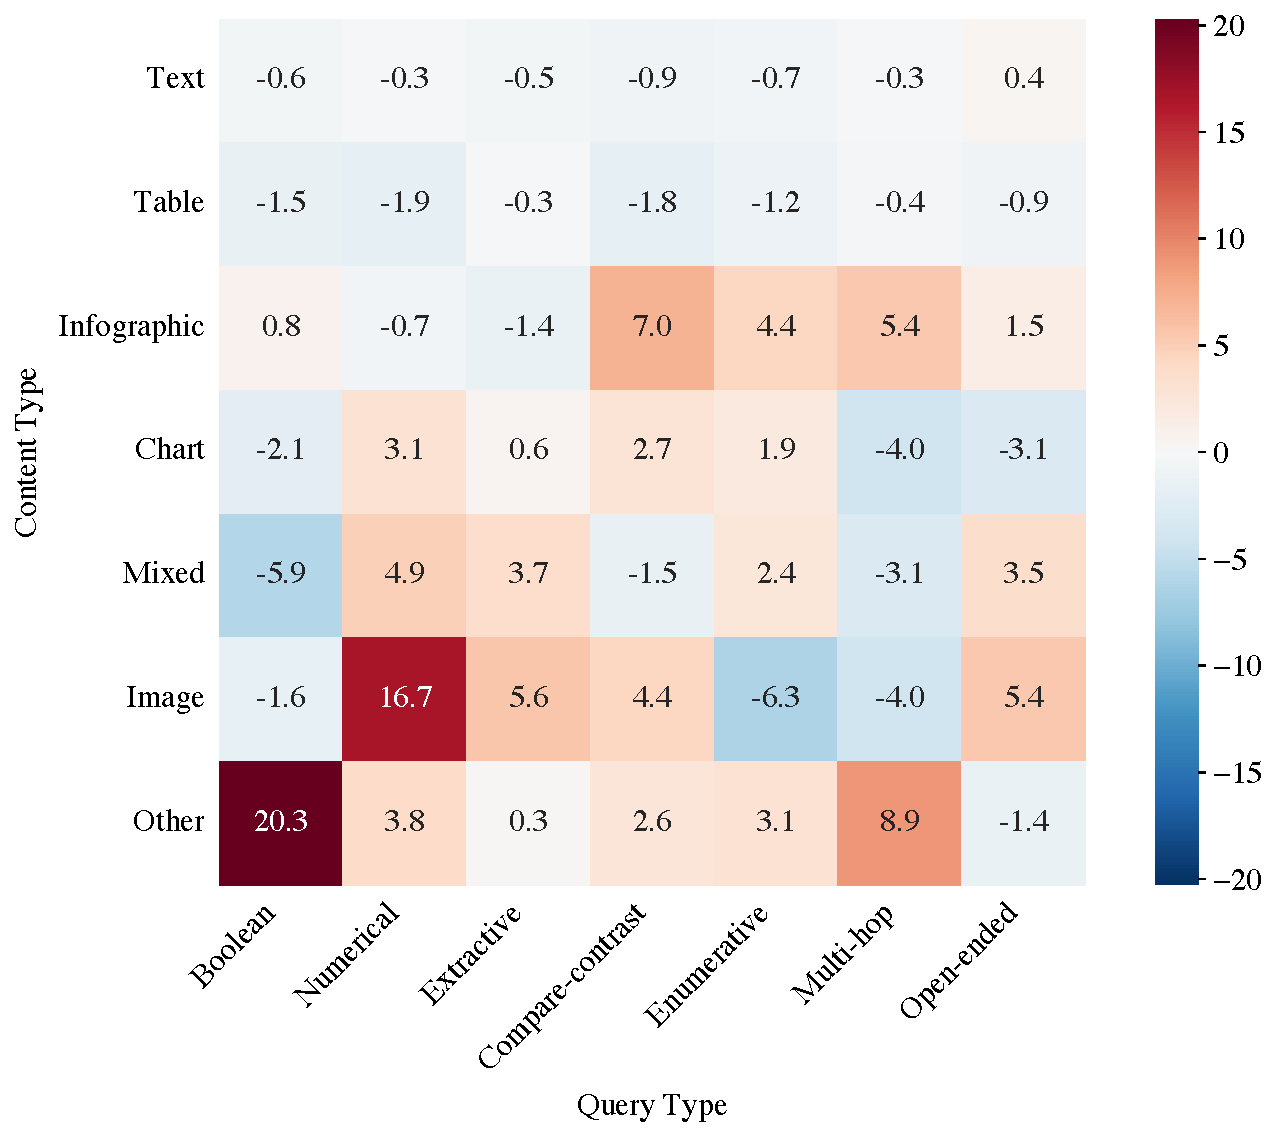
\includegraphics[width=\columnwidth]{images/vidorev3_images/ndcg_content_query_residuals_heatmap.pdf}
\caption{\textbf{Residuals from additive performance model.} Each cell shows the difference between observed NDCG@10 and the value predicted by an additive model of query type and content type main effects. Values near zero (white) indicate no interaction; positive values (red) indicate better-than-expected performance for that combination; negative values (blue) indicate worse-than-expected.} 
\label{fig:ndcg content query residuals heatmap}
\end{figure}

% \begin{table}[h!]
% \centering
% \resizebox{\columnwidth}{!}{%
% \begin{tabular}{lcc}
% \toprule
% Query format & NDCG@10 & Query count \\
% \midrule
% Question & 62.6 & 9936 \\
% Keyword & 56.4 & 2988 \\
% Instruction & 55.6 & 5670 \\
% \bottomrule
% \end{tabular}
% }
% \caption{\textbf{ColEmbed-3B-v2 NDCG@10 by query format.}}
% \label{tab:perf query format}
% \end{table}

% \begin{table}[h!]
% \centering
% \resizebox{\columnwidth}{!}{%
% \begin{tabular}{lcc}
% \toprule
% Query type & NDCG@10 & Query type count \\
% \midrule
% Boolean & 70.3 & 2250 \\
% Numerical & 66.3 & 3540 \\
% Extractive & 65.8 & 6528 \\
% Compare-contrast & 60.0 & 3162 \\
% Enumerative & 57.6 & 2790 \\
% Multi-hop & 53.9 & 1728 \\
% Open-ended & 48.6 & 5628 \\
% \bottomrule
% \end{tabular}
% }
% \caption{\textbf{colembed-3b-v2 NDCG@10 by query type.} The sum of the query type count column exceeds the number of individual queries since a query may have multiple tags,}
% \label{tab:perf query type}
% \end{table}

% \begin{table}[h!]
% \centering
% \resizebox{\columnwidth}{!}{%
% \begin{tabular}{l ccc c}
% \toprule
% & \multicolumn{3}{c}{\textbf{Query Format}} & \\ % Labels the columns
% \cmidrule(lr){2-4}
% \textbf{Query Type} & Instruction & Keyword & Question & \textbf{Mean} \\
% \midrule
% Boolean & — & — & 70.3 & 70.3 \\
% Numerical & 65.0 & 64.9 & 67.6 & 66.3 \\
% Extractive & 63.3 & 65.6 & 67.3 & 65.8 \\
% Compare-contrast & 59.3 & 59.2 & 61.3 & 60.0 \\
% Enumerative & 56.2 & 65.2 & 57.8 & 57.6 \\
% Multi-hop & 50.6 & — & 57.1 & 53.9 \\
% Open-ended & 48.0 & 45.8 & 50.6 & 48.6 \\
% \midrule
% \textbf{Mean} & 55.6 & 56.4 & 62.6 & 59.5 \\
% \bottomrule
% \end{tabular}
% }
% \caption{\textbf{colembed-3b-v2 NDCG@10 by query type and format.} The sum of the query type counts exceeds the number of individual queries since a query may have multiple tags.}
% \label{tab:perf query type format}
% \end{table}

% \begin{table}[h!]
% \centering
% \resizebox{\columnwidth}{!}{%
% \begin{tabular}{lcc}
% \toprule
% Content type & NDCG@10 & Content type count \\
% \midrule
% Text & 59.3 & 17244 \\
% Chart & 56.3 & 2364 \\
% Infographic & 55.2 & 2814 \\
% Table & 53.9 & 6480 \\
% Other & 50.8 & 492 \\
% Image & 49.3 & 1140 \\
% Mixed & 45.1 & 1164 \\
% \bottomrule
% \end{tabular}
% }
% \caption{\textbf{ColEmbed-3B-v2 NDCG@10 by content type.} Content type is labeled on each annotated page based on the nature of the query-relevant content delimited by the bounding boxes.}
% \label{tab:perf content type}
% \end{table}

% \begin{table}[h!]
% \centering
% % \resizebox{\columnwidth}{!}{%
% \begin{tabular}{lcc}
% \toprule
% Number of pages & NDCG@10 & Query count \\
% \midrule
% 1 & 76.4 & 4794 \\
% 2 & 64.7 & 3234 \\
% 3 & 60.5 & 1902 \\
% 4 & 58.7 & 1560 \\
% 5-9 & 48.5 & 4398 \\
% 10-19 & 41.2 & 2280 \\
% 20+ & 39.0 & 426 \\
% \bottomrule
% \end{tabular}
% % }
% \caption{\textbf{colembed-3b-v2 NDCG@10 by number of annotated pages.}}
% \label{tab:perf number of pages}
% \end{table}



% \begin{table}[h!]
% \centering
% \resizebox{\columnwidth}{!}{%
% \begin{tabular}{l c c}
% \toprule
% Generation method & NDCG@10 & Query count \\
% \midrule
% Summary + synthetic & 51.6 & 7992 \\
% Summary + human & 55.4 & 4590 \\
% Page images + human & 73.1 & 6012 \\
% \bottomrule
% \end{tabular}
% }
% \caption{\textbf{ColEmbed-3B-v2 NDCG@10 by query generation method.}}
% \label{fig:perf query generation method}
% \end{table}

\section{Bounding box annotations}
\label{appendix: bbox}

\paragraph{Inter-annotator agreement} \label{appendix: annotator agreement bbox}

Table~\ref{tab:inter-annotator bbox agreement} shows IoU and F1 scores between human annotations, to detail results of Section~\ref{sec: grounded qa}.

\begin{table*}[h!]
\centering
\resizebox{\textwidth}{!}{%
\begin{tabular}{l c c c c c c c c c c >{\columncolor{avgcol}}c}
\toprule
 & \multicolumn{7}{c}{\textbf{English Datasets}} & \multicolumn{3}{c}{\textbf{French Datasets}} & \multicolumn{1}{c}{} \\
\cmidrule(lr){2-8} \cmidrule(lr){9-11}
\textbf{Metric} & C.S. & Nucl. & Fin. & Phar. & H.R. & Ind. & Tele. & Phys. & Ener. & Fin. & \textbf{Average} \\
\midrule
\textbf{IoU} & 0.500 & 0.476 & 0.462 & 0.615 & 0.474 & 0.502 & 0.526 & 0.443 & 0.470 & 0.503 & \textbf{0.497} \\
\textbf{F1} & 0.608 & 0.594 & 0.569 & 0.720 & 0.594 & 0.611 & 0.637 & 0.540 & 0.569 & 0.581 & \textbf{0.602} \\
\bottomrule
\end{tabular}
}
\caption{\textbf{Inter-annotator agreement metrics on bounding box annotations.}}
\label{tab:inter-annotator bbox agreement} 
\end{table*}

\paragraph{Bounding box predictions}

Figure~\ref{fig:bbox_instructions} shows the prompt used to generate final answers with inline bounding boxes for visual grounding, and Figure~\ref{fig:bbox evaluation} reports bounding box localization F1 scores by dataset.

\begin{figure*}[h!]
    \centering
    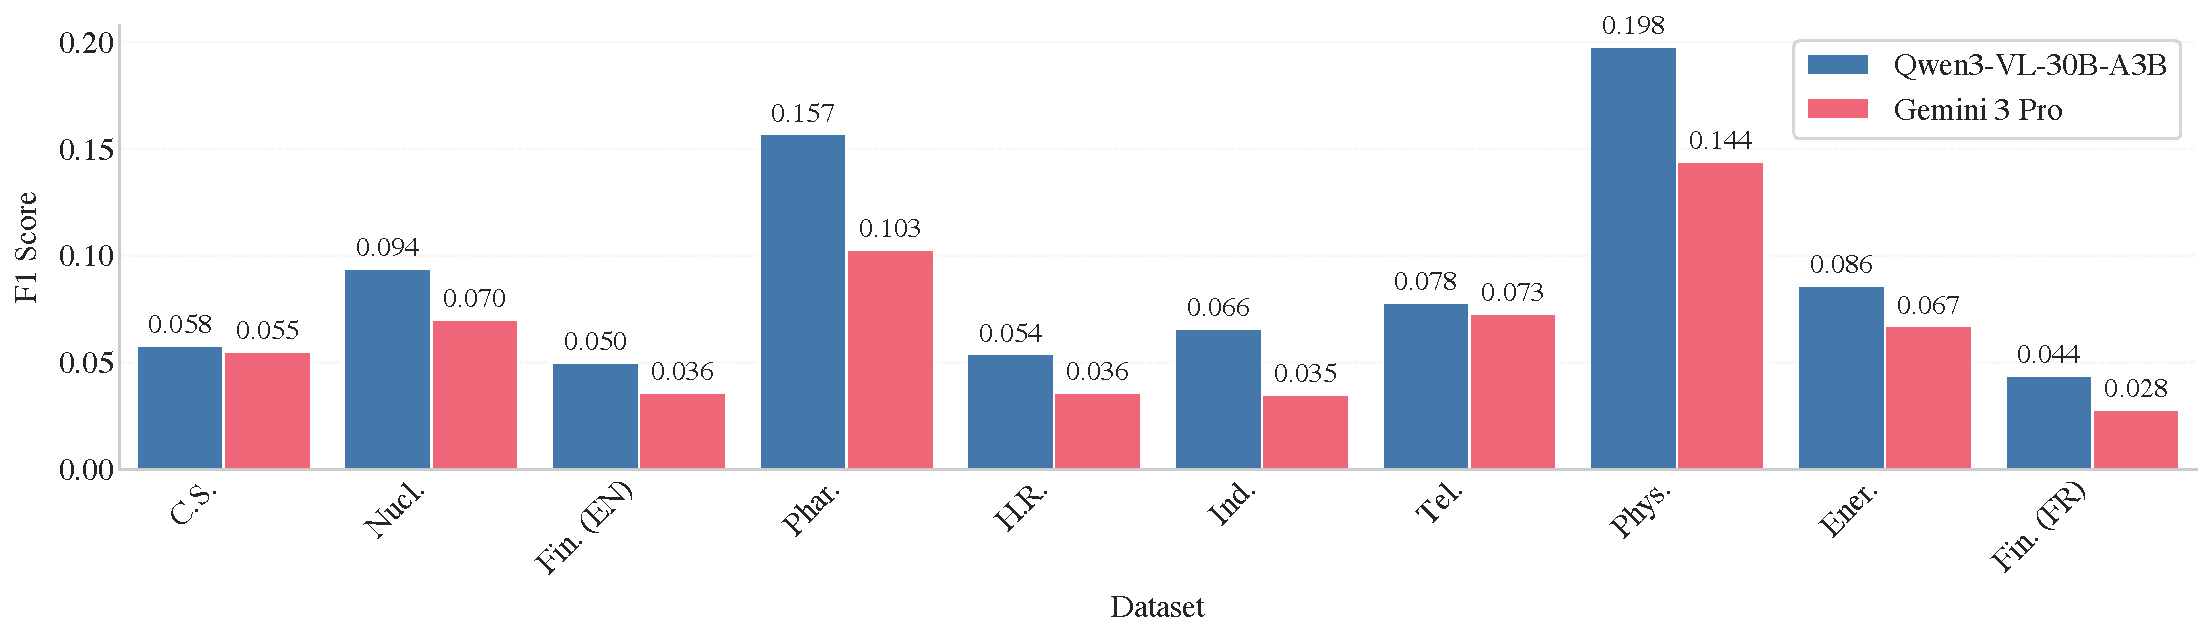
\includegraphics[width=\textwidth]{images/vidorev3_images/bbox_localization_by_dataset.pdf}
    \caption{\textbf{Model bounding box localization performance}. Each F1 score measures the zone-based overlap between model-generated bounding boxes and human annotations, using the annotator yielding the highest F1.} 
    \label{fig:bbox evaluation}
\end{figure*}

\section{Final answer evaluation} \label{appendix:final answer eval}

\paragraph{Evaluation setup} Generated final answers are evaluated in a pass@1 setting using GPT 5.2 with medium reasoning effort as the LLM judge. The judge compares each generated answer against the ground-truth annotation and returns a binary correctness label. The answer generation and judge prompts are shown in Figure~\ref{fig:generation_prompt} and Figure~\ref{fig:judge_prompt} respectively. We evaluated Gemini 3 Pro with low thinking effort, GPT-5 with medium reasoning effort, as well as the thinking version of Qwen3-VL-235B-A22B.

% To assess the variance of this evaluation, we conducted 5 independent runs on Gemini 3 Pro outputs using the oracle retriever with image context. Individual run scores were 71.72\,\%, 72.14\,\%, 72.14\,\%, 72.14\,\%, and 72.30\,\%, for a mean score of 72.09\,\% and a standard deviation of 0.22\,\% ((Krippendorff's $\alpha = 0.91$, indicating high intra-judge consistency).

To assess the reliability of our judge, we conducted 5 independent evaluation runs on a fixed set of Gemini 3 Pro outputs. Individual run scores showed minimal fluctuation (mean 72.09\,\%, $\sigma=0.22$\,\%) and high internal consistency (Krippendorff's $\alpha = 0.91$), confirming that the judge is consistent given a fixed context.

\paragraph{End-to-End Pipeline Stability} While the judge demonstrates high consistency on fixed inputs, the full evaluation pipeline introduces a second layer of variability: the model's generation process. To quantify the end-to-end variance under rigorous conditions, we performed 5 independent runs. For computational efficiency, we restricted this stress test to the most challenging corpus in each language: \textit{Industrial Maintenance} (English) and \textit{Finance} (French).

We measured an average score of 65.74\,\% with a standard deviation of 0.94\,\%. Crucially, the evaluation signal remains robust against generative noise, achieving a Krippendorff's $\alpha$ of 0.80. This agreement confirms that the end-to-end results are statistically reliable even when subjected to the most difficult evaluation scenarios.

\paragraph{Easy/hard query filtering} To classify queries by difficulty, we prompt a panel of 6 LLMs to answer each query without access to any corpus context. We select GPT-5-nano, GPT-5-mini, GPT-5, Qwen3-VL-30B-A3B, Gemini 2.5 Flash, and Gemini 2.5 Pro to span different model families and capability levels. Each model receives only the query text and is asked to provide a direct answer with the prompt in Figure~\ref{fig:easy_query_prompt}. Answers are evaluated for correctness using the same GPT-5.2 judge described above. A query is labeled \textit{easy} if at least one model answers correctly, and \textit{hard} otherwise. Table~\ref{tab: easy hard filtering} reports per-model accuracy and the resulting proportion of easy queries for each dataset. The distribution varies substantially across domains: knowledge-intensive datasets such as Computer Science and Physics have over 85\% easy queries, while domain-specific datasets such as Finance and Energy contain fewer than 35\% easy queries, reflecting the specialized nature of their content.


% \begin{table*}[h!]
% \centering
% \begin{tabular}{l c c c c c c c c >{\columncolor{avgcol}}c}
% \toprule
%  & \multicolumn{5}{c}{\textbf{English Datasets}} & \multicolumn{3}{c}{\textbf{French Datasets}} & \multicolumn{1}{c}{} \\
% \cmidrule(lr){2-6} \cmidrule(lr){7-9}
% \textbf{\# Queries} & C.S. & Fin. & Phar. & H.R. & Ind. & Phys. & Ener. & Fin. & \textbf{Total} \\
% \midrule
% Original    & 215 & 309 & 364 & 318 & 283 & 302 & 308 & 320 & 2419 \\
% Remaining   & 29  & 211 & 156 & 202 & 173 & 41  & 208 & 224 & 1244 \\
% \bottomrule
% \end{tabular}
% \caption{\textbf{\textit{Hard} query filtering statistics}. We report the original query counts versus the number of \textit{hard} queries remaining after filtering for model consensus.}
% \label{tab: hard queries answer generation}
% \end{table*}

\begin{table*}[h!]
\centering
\label{tab:performance_model}
% \resizebox{\textwidth}{!}{%
\begin{tabular}{l c c c c c c c c >{\columncolor{avgcol}}c}
\toprule
 & \multicolumn{5}{c}{\textbf{English Datasets}} & \multicolumn{3}{c}{\textbf{French Datasets}} & \multicolumn{1}{c}{} \\
\cmidrule(lr){2-6} \cmidrule(lr){7-9}
\textbf{Model} & C.S. & Fin. & Phar. & H.R. & Ind. & Phys. & Ener. & Fin. & Total \\
\midrule
GPT-5-nano     & 74.4 & 7.4  & 30.5 & 12.9 & 15.6 & 74.2 & 14.0 & 9.1  & 29.8 \\
GPT-5-mini      & 79.1 & 13.3 & 37.4 & 17.6 & 20.5 & 80.1 & 13.6 & 13.1 & 34.3 \\
GPT-5           & 76.3 & 25.2 & 50.8 & 29.9 & 32.2 & 80.5 & 26.0 & 22.2 & 42.9 \\
Qwen3-VL-30B-A3B & 60.9 & 3.9  & 19.2 & 6.3  & 9.9  & 60.9 & 6.8  & 4.4  & 21.5 \\
Gemini 2.5 Flash& 66.1 & 8.7  & 30.8 & 13.5 & 15.9 & 63.6 & 14.9 & 13.1 & 28.3 \\
Gemini 2.5 Pro  & 70.2 & 16.8 & 29.4 & 15.4 & 23.7 & 63.9 & 20.5 & 20.0 & 32.9 \\
\midrule
\textbf{Easy queries (\%)}           & 86.5 & 31.7 & 57.1 & 36.5 & 38.9 & 86.4 & 32.5 & 30.0 & 48.6 \\
\bottomrule
\end{tabular}
% }
\caption{\textbf{Percentage of queries correctly answered by LLMs without corpus context.} A panel of 6 LLMs is asked to answer the queries of the 8 public datasets without access to any corpus context. Queries correctly answered by at least one of the 6 models are classified as \textit{easy} queries, while the rest are labeled as \textit{hard}. Easy queries account for 48.6\,\% of all the queries.}
\label{tab: easy hard filtering}
\end{table*}


\clearpage

\section{Visual grounding examples}

% Merge of the 2 paragraphs below:

Qualitative analysis reveals distinct failure modes. Gemini frequently produces off-by-one page indexing errors: the predicted coordinates would correctly localize the target content if applied to an adjacent page. The two models also differ in box granularity: Gemini tends to draw tight boxes around individual elements (e.g., a single table cell or text line), whereas Qwen3-VL generates larger boxes encompassing entire sections or paragraphs, more closely matching human annotation patterns. Figures~\ref{fig:bbox examples qwen} and~\ref{fig:bbox examples gemini} illustrate these tendencies across four dataset pages: Qwen3-VL's bounding boxes are comparatively wide and encompass entire page elements (pages (a), (c), and (d)), while Gemini 3 Pro's visual grounding is more precise (pages (b) and (c)). This difference in granularity partially explains Qwen3-VL's higher F1 scores, as broader boxes are more likely to overlap with the ground-truth zones used in our evaluation. Both models exhibit errors and omissions: in page (b), the chart is not labeled by Qwen3-VL, and in page (d), Gemini 3 Pro predicts incorrect bounding boxes for the bottom table while Qwen3-VL provides grounding for the wrong table.

%Qualitative analysis reveals distinct failure modes. Gemini frequently produces off-by-one page indexing errors: the predicted coordinates would correctly localize the target content if applied to an adjacent page. The two models also differ in box granularity: Gemini tends to draw tight boxes around individual elements (e.g., a single table cell or text line), whereas Qwen3-VL generates larger boxes encompassing entire sections or paragraphs, more closely matching human annotation patterns \gmor{If we need to save some space for submission, these details about how Gemini and Qwen3-VL generates boxes could go to the Appendix}. This difference partially explains Qwen3-VL's higher F1 scores, as broader boxes are more likely to overlap with the ground-truth zones used in our evaluation.

%Figures~\ref{fig:bbox examples qwen} and~\ref{fig:bbox examples gemini} show examples of bounding box predictions by Qwen3-VL-30B-A3B and Gemini 3 Pro for 4 dataset pages. They show examples of the qualitative behavior of the models we observe throughout the dataset. Qwen3-VL's bounding boxes tend to be comparatively wide and encompass entire page elements, as seen in pages (a), (c) and (d), while Gemini 3 Pro's visual grounding is more precise (pages (b) and (c)). We also include evidence of errors and omissions from these two models: in page (b), the chart is not labeled by Qwen3-VL and in page (d), Gemini 3 Pro predicts wrong bounding boxes for the bottom table, while Qwen3-VL provides grounding for the wrong table.

\begin{figure*}[h!]
    \centering
    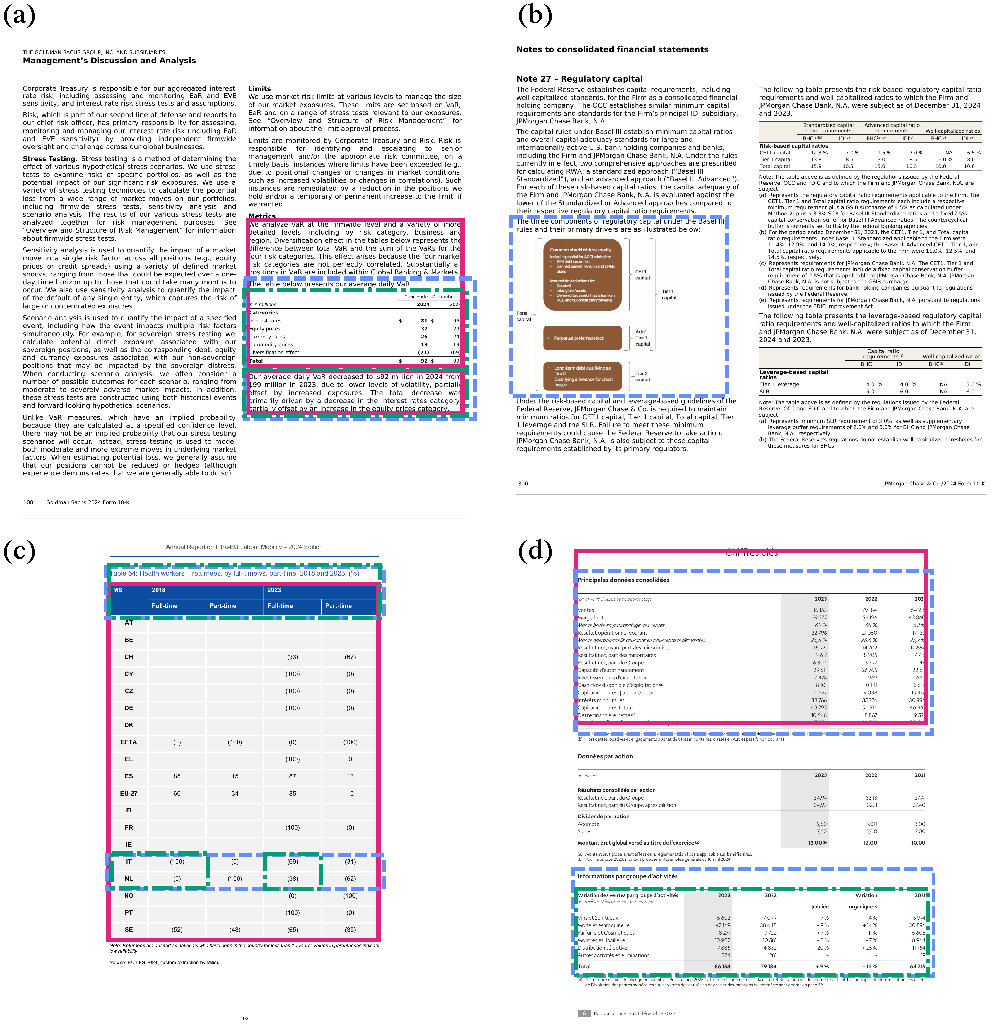
\includegraphics[width=\textwidth]{images/vidorev3_images/bbox_examples_qwen.pdf}
    \caption{\textbf{Visual grounding comparative examples for Qwen3-VL-30B-A3B.} Each panel shows a document page with Qwen3-VL's predicted bounding boxes (solid magenta) and human bounding boxes (dashed blue and green, one color per annotator). Corresponding datasets and queries: (a) finance\_en: What was the average daily Value at Risk (VaR) for Goldman Sachs during 2024?, (b) finance\_en: List the 3 components of regulatory capital under Basel III, and determine the role of each component., (c) hr\_en: Analyze how full-time employment among returning health workers evolved in the Netherlands and Italy from 2018 to 2023, and describe the differences in their employment trends., (d) finance\_fr: Croissance Mode Maroquinerie vs Vins Spiritueux 2023 performance}
    \label{fig:bbox examples qwen}
\end{figure*}

\begin{figure*}[h!]
    \centering
    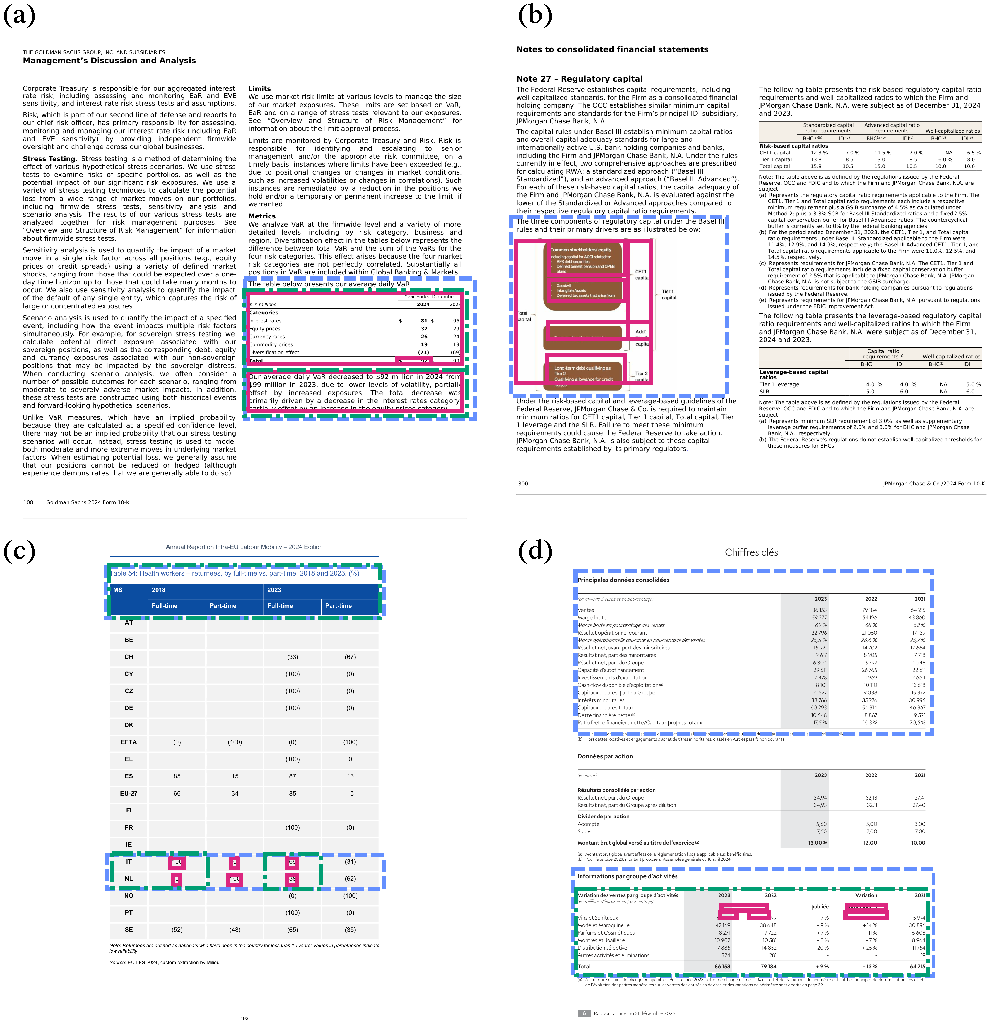
\includegraphics[width=\textwidth]{images/vidorev3_images/bbox_examples_gemini.pdf}
    \caption{\textbf{Visual grounding comparative examples for Gemini 3 Pro.} Each panel shows a document page with Gemini's predicted bounding boxes (solid magenta) and human bounding boxes (dashed blue and green, one color per annotator). Corresponding datasets and queries: (a) finance\_en: What was the average daily Value at Risk (VaR) for Goldman Sachs during 2024?, (b) finance\_en: List the 3 components of regulatory capital under Basel III, and determine the role of each component., (c) hr\_en: Analyze how full-time employment among returning health workers evolved in the Netherlands and Italy from 2018 to 2023, and describe the differences in their employment trends., (d) finance\_fr: Croissance Mode Maroquinerie vs Vins Spiritueux 2023 performance}
    \label{fig:bbox examples gemini}
\end{figure*}

\label{appendix: bbox examples}

% \clearpage

\section{Instructions given to Annotators}
\label{appendix: annotator_instructions}

\paragraph{Query Generation}\Cref{fig:task_1_instructions} details step-by-step instructions to annotators to generate queries from summaries and images.

\begin{promptfigure}[blue!5]{\textbf{Instructions given to human annotators to create queries}}{fig:task_1_instructions}
\begin{verbatim}
# Step 1
    The annotator will be provided with content(text summary or image(s)) and a list of instructions
    on the queries that are expected.

# Step 2
    Read and analyse the content.

# Step 3
    - The annotator writes a series of queries that can, supposedly, be answered by the summarized
    content. It is okay if the information needed to answer the question is in other parts of the
    document or not explicitly written in the summary.
    - If the summary is not adapted to a specific type or format of questions, the annotator may skip. 
    - They should follow the number of queries asked for each category.
    - They should follow the expected type of queries provided and the format.
\end{verbatim}
\end{promptfigure}


\paragraph{Query-Page Relevancy linking}\Cref{fig:task_2_instructions} details the step-by-step instructions provided to annotators for assessing page relevance, identifying content modalities, and localizing evidence via bounding boxes. \Cref{tab:relevance_scale} gives the definitions of relevancy scores used by the human annotators.

\begin{table}[h!]
\centering
\small
% Removed vertical bars (|) from the column definition
\begin{tabularx}{\columnwidth}{clX} 
\toprule
\textbf{Score} & \textbf{Label} & \textbf{Definition} \\
\midrule
2 & Fully Relevant & The page contains the complete answer. \\ 
\addlinespace % Adds a nice breathing room between rows without breaking lines
1 & Critically Relevant & The page contains facts or information required to answer the query, though additional information is required. \\ 
\addlinespace
0 & Not Relevant & Provides no information relevant to the query. \\
\bottomrule
\end{tabularx}
\caption{\textbf{Relevance definitions used for page-level annotations.}}
\label{tab:relevance_scale}
\end{table}

% \begin{table*}[h!]
% \centering
% \small
% \begin{tabular}{clp{7cm}}
% \toprule
% \textbf{Score} & \textbf{Label} & \textbf{Definition} \\
% \midrule
% 2 & Fully Relevant & The page contains the complete answer \\
% 1 & Critically Relevant & The page contains facts or information required to answer the query, though additional information is required \\
% 0 & Not Relevant & Provides no information relevant to the query \\
% \bottomrule
% \end{tabular}
% \caption{\textbf{Relevance scale used for page-level annotations.}}
% \label{tab:relevance_scale}
% \end{table*}

\begin{promptfigure}[blue!5]{\textbf{Instructions given to human annotators to annotate query-page relevancy}}{fig:task_2_instructions}
\begin{verbatim}
# Task overview
In this task, the annotator will be provided with a query and pages that are supposed to be relevant
to answer the query. The annotator’s goal is to rate the relevance in answerability of each page with
respect to the query.

# Step 1:
    - Review the query and pages to get an understanding of the content and domain
    
# Step 2:
    Rate the query quality. 
    - If adheres to guidelines > Good (1)
    - If doesn’t adhere to guidelines> Poor(0)
    - If the query is Poor quality, skip the task.
    
# Step 3:
    - For each page, rate the relevance with respect to the query
    - If page completely answer query > Fully Relevant(2)
    - If page contains information required to answer the query > Critically Relevant(1)
    - If page contains no relevant information > Not Relevant(0)
    
# Step 4:
    - For each page, annotate the modalities in which the relevant information is located concerning
    the query-page link, relevant information can be located in multiple modalities at the same time:
Modality : [“text”, “table”, “chart”, infographic”, “image”, “other”]
    - If relevance score = 0, modality may be “N/A”
    
# Step 5:
    - For each page, draw bounding boxes around the relevant text/chart/image/infographic (if any)
    - If relevance score = 0, do not draw a bounding box
    
# Step 6:
    - Repeat steps 3, 4 and 5 for all pages
    
# Step 7:
    - Propose an answer to the query, given the relevant pages.
    - If the query is not answerable, rate it as “unanswerable”

\end{verbatim}
\end{promptfigure}

\section{Prompts}

All the prompts used for both dataset generation and evaluations are detailed from \Cref{fig:query_generation_prompt} to \Cref{fig:bbox_instructions}.

\begin{promptfigure}{\textbf{Prompt used generate synthetic queries with the NeMo Data Designer tool}}{fig:query_generation_prompt}
\begin{verbatim}
<mission>
You are an assistant specialized in visual document understanding tasks. You will be given a context, 
summarizing the content of a section or multiple document sections. Your goal is to carefully analyze 
the context and to solve a series of tasks related to its content. You are tasked with generating 
query-answer pairs. Your queries will be used to simulate a user unfamiliar with the specific content 
of the page, and who is looking for information in a large knowledge base through a search engine. 
The user does not have access to the document and is looking for information that can be present in 
any document in the knowledge base.
</mission>

<definitions>
- A query is said to be fully answerable if the page contains a precise and complete answer to the 
query.
- A query is said to be partially answerable if the page contains relevant information that is 
directly related to the query but some key information is missing and must be retrieved in other 
pages or documents in order to give a precise and complete answer.
- An open-ended query is an explanatory or descriptive query that synthesizes  information; may be 
broad in scope and focused on qualitative aspects of the summary
- A compare-contrast query is a query that requires comparing and/or contrasting multiple entities or 
topics that are closely related to each other
- An enumerative query is a query that asks to list all examples that possess a common property, 
optionally requesting details about the specifics of each example.
- A numerical query is a query that asks for a specific number or calculated number given a summary. 
The query should require more than simply reading numbers directly from the page.
- A boolean query is a yes/no query that may involve multiple steps of reasoning.
- An extractive query is a clear and specific query that can be answered using only a specific piece 
of information.
- A multi-hop query is a complex query that requires retrieving and integrating information from 
multiple sources or steps to produce a complete answer.
- A question query is a complete sentence that ends with a question mark, typically used to seek 
specific information or clarification.
- A keyword query is a brief, often fragmented phrase or set of terms used to search or filter 
information, without forming a full grammatical sentence.
- An instruction query is a directive that describes a task to be performed on the documents, often in 
the form of a command or request.
</definitions>
<rules>
<queries>
- Generate queries only in {{ language }}.
- Make queries diverse, natural, and plausible for someone unfamiliar with the document.
- Each query must be standalone; do not reference “the page”, “the table”, “the figure”, 
“the document”, “the text”, “the table of contents”, etc.
- Rephrase; avoid copying wording from the source so semantic matching, not surface matching, 
is tested.
- You may include queries about relationships or trends often shown in images/vidorev3_tables/images/vidorev3_images/graphs, 
but never refer to a specific table/figure.
- Avoid overly generic queries that apply to any document.
- Keep each query concise ({{ length }} words).
- When appropriate, write multi-hop queries that integrate information across the provided pages.
</queries>
</rules>
<instructions>

Used Documents: {{ document_names }}
<summary>
{{summary}}
</summary>
Using the provided context, generate a {{ difficulty }}, {{ reasoning_type }}, {{ answerability }}
query. The query should be {{ query_type }} using the provided context and have the format of a 
{{ query_format }} query.
The query should be self-sufficient and related to the context.
</instructions>
\end{verbatim}
\end{promptfigure}

\begin{promptfigure}{\textbf{Prompt used to pre-filter the irrelevant pages for a given query}}{fig:query_linking_prompt}

\begin{verbatim}
<mission>
You are an assistant specialized in visual document understanding tasks. You will be given a document
page by page and a question. Your goal is to carefully analyze the page and say if it is related to
the question's answer. You are tasked with generating question-page affiliation as well as the
question answer if it exists in the page. 
</mission>

<definitions>
- A question is said to be fully answerable if the corresponding page contains a precise and complete
answer to the question.
- A question is said to be partially answerable if the corresponding page content is necessary to
answer the question but some key information is missing.
- A question is said to be unanswerable if the corresponding page contains information related to the
question's topic or domain but upon closer inspection does not contain information that is useful to
answer the question. Or if the page has no link whatsoever with the query.
</definitions>

<rules>
<page_affiliation>
- Be sure to put the relevance (and only that) between the tags <relevance>...</relevance>.
The possible values are: 
    <relevance>fully answerable</relevance>,
    <relevance>partially answerable</relevance>
    <relevance>unanswerable</relevance>.
- Be very careful when doing your page affiliation. Only say a page is relevant when it really is.
</page_affiliation>
<answers>
- You must generate the answer between the tags <answer>...</answer>. Between these tags, you should
only put the answer to the question.
- You must generate answers in the following language: {language}
- Your answers should be complete sentences.
- When the question is ambiguous, your answer should state that there is an ambiguity in the question.
- You should always generate the answer based on all the information available on the page, even if
the question was generated only on part of the page.
</answers>
</rules>

<instructions>
Return if the following question is "fully answerable" "partially answerable" or "unanswerable" based
on the content of the page between the tags <relevance> ... </relevance>. 
If the question is answerable, provide the answer.

Here is the question :
{{ query }}

And there is the page content :

</instructions>
\end{verbatim}
\end{promptfigure}

\begin{promptfigure}{\textbf{Prompt used to merge human annotators answers}}{fig:answer_merging_prompt}
\begin{verbatim}
You are given a set of document pages (images), a query, and a list of one or more
proposed answers.

Query :

{{ query }}

Proposed Answers:

{{ answers }}

Your task is to carefully analyze the provided pages, the query, and the proposed answers. You must
return a single, syntactically correct JSON object with the following structure:
```json
{
    "reasoning": "<string>",
    "information_in_pages": <true or false>,
    "answer_correctness": [<true or false>, ...],
    "reformulated_answer": "<string>"
}
```
Instructions for each field:
- reasoning: Explain the logic for each boolean in the `answer_correctness` list.
For each proposed answer, state why it is correct or incorrect, citing specific  evidence from the
document pages.

- information_in_pages: Set to `true` if the information needed to definitively answer the query
is present in the pages. Otherwise, set to `false`.

- answer_correctness: A list of booleans, corresponding to each proposed answer  in the original
order. Use `true` if the answer is verifiably correct based on the pages and `false` otherwise.

- reformulated_answer: A single string containing the most precise and correct answer to the query,
derived only from information in the pages. If any of the proposed answers are correct, use them as
a basis for synthesizing this improved answer. The reformulation must be concise and factual.

Important rules:
- Base your entire analysis strictly on the content of the provided document pages. 
Do not use outside knowledge.

- Do not invent, infer, or assume information that is not explicitly stated in the pages.

- Always provide a string for the `reformulated_answer`, even if no correct answer can be formed
from the text.

- Your final output must be only the JSON object.
\end{verbatim}
\end{promptfigure}

\begin{promptfigure}{\textbf{Easy/hard query filtering prompt}}{fig:easy_query_prompt}
\begin{verbatim}
Give a very precise and concise answer to the following query.
If you are unable to answer, output 'I don't know'.
Query: {{ query }}
\end{verbatim}
\end{promptfigure}

\begin{promptfigure}{\textbf{Judge prompt used for end to end evaluation}}{fig:judge_prompt}
\begin{verbatim}
You are an expert judge evaluating the accuracy of a test answer against a gold-standard true answer.
Your goal is to determine if the test answer captures the essential "core information."

### Evaluation Criteria:
- Correct: The test answer contains all core information of the true answer. Minor omissions of
non-essential details or the addition of minor, non-contradictory information should still be marked
as "Correct."
- Partially Correct: The test answer captures some of the core information, but suffers from
significant omissions or includes substantial extra information that was not requested or present in
the true answer.
- Incorrect: The test answer is fundamentally wrong, contradicts the true answer, or misses the core
information entirely.

### Input Data:
Query: {{ query }}

True Answer: {{ true_answer} }

Test Answer: {{ test_answer }}

### Output Format:
Provide a very brief explanation for your judgment. You must output your final response in a JSON
format with two fields: "explanation" and "judgment" (which must be "Correct", "Partially Correct",
or "Incorrect").
\end{verbatim}
\end{promptfigure}

\begin{promptfigure}{\textbf{Answer generation prompt used for end to end evaluation}}{fig:generation_prompt}
\begin{verbatim}
You are an expert at answering query based on documents.

Here is a list of relevant documents: {{ documents }}

Based on the above documents, answer the following query: {{ query }}

Keep the response short when appropriate. Output the answer only.
\end{verbatim}
\end{promptfigure}

\begin{promptfigure}{\textbf{Query translation from English to French prompt}}{fig:query_translation}
\begin{verbatim}
English text to translate: {{ query }}

Translate the English text above to French.
Make sure you follow the format of the English text. Don't change acronyms.
Follow the following json schema.
{
    "french_translation": ...
}
\end{verbatim}
\end{promptfigure}

\begin{promptfigure}{\textbf{Bounding box prediction prompt}}{fig:bbox_instructions}
\begin{verbatim}
# Role and Objective
- Serve as an expert in document analysis and visual grounding.
- Given a query and multiple document page images, provide a natural language answer with inline
grounding references.

# Instructions
- Analyze all provided pages to answer the query comprehensively.
- For each piece of information used in your answer, provide visual grounding by including bounding
box coordinates of all the sections of the document that help answer the query.
- Use this format to include the list of all bounding boxes of image N:
<bboxes image="N">[[x_{min}, y_{min}, x_{max}, y_{max}], ...]</bboxes>
  - image="N" specifies the 0-indexed page number (0=first page, 1=second page, etc.)
  - Include bounding boxes inline in your answer, immediately after mentioning the relevant
  information
  - A given page may contain multiple non-contiguous sections that help answer the query. In this
  case, you must output the list of the bounding boxes of all these sections.
  - You must group all the bounding boxes of a given page into a single 
    <bboxes image="N">...</bboxes> tag.

# Grounding Principles
- DO NOT output more than 5 bounding boxes per page.
- Adjacent logical units must be enclosed in a single, continuous bounding box.
- Return multiple bounding boxes only if information is clearly independent and separated by
significant non-relevant content.

# Output Format
- Provide a natural language answer to the query.
- Embed grounding tags directly inline where relevant information is discussed.
- Example: "The valuation technique described on page 1 
  <bboxes image="0">[[120, 450, 890, 670], [100, 800, 330, 960]]</bboxes> 
  uses discounted cash flow analysis."
\end{verbatim}
\end{promptfigure}

% \chapter{ModernVBert Appendix}


% Appendix
\section{Training}

\subsection{Implementation and Resources}
\label{appendix:implementation_details}
\begin{table*}[ht]
\centering
\resizebox{\textwidth}{!}{%
\begin{tabular}{l r r r r}
  \toprule
  Model & Batch Size & Learning Rate & Training Steps & Training GPU Hours \\
  \midrule
  \multicolumn{5}{l}{\textbf{Modality Alignment}} \\
  \flagshipbase{} (Table~\ref{tab:mod_alignment_mix}) & 4096 & 1e-4 & 5500 & 1920h \\
  \midrule
  \multicolumn{5}{l}{\textbf{Contrastive Learning}} \\
  Generalist contrastive training (Table~\ref{tab:cl_mix}) & 256 & 2e-4 & 3917 & 80h \\
%  \texttt{colmodernvbert-embed} & — & - & - & - \\ 
  \midrule
  \multicolumn{5}{l}{\textbf{Document Specialization}} \\
  Document-focused contrastive training w/ hard negatives (Table~\ref{tab:cl_mix}) & 64 & 2e-4 & 19602 & 160h \\
  \bottomrule
\end{tabular}
}
\caption[Training details by stage]{Training details of our final models at each training stage. GPU Hours are on 80GB H100 GPUs.}
\label{table:app_training_details}
\end{table*}

% We list the details of each MetaEmbed variant in Table 4. We reserve 1% training data from each subset of MMEB-train as evaluation split and training was early stopped when evaluation loss stops dropping. All models are trained with gradient checkpointing (Chen et al., 2016) to reduce memory usage. Training was conducted using PyTorch (Paszke et al., 2019) 2.6.0+cu124 and FlashAttention 2.0 (Dao, 2024). For the 3B configuration, we adopt Distributed Data Parallel (Li et al., 2020) while for all other model sizes we use Fully Sharded Data Parallel (FSDP) (Zhao et al., 2023) v2. To prevent distributed hanging when training samples contain no images under FSDP, we pad those samples with a placeholder image to ensure the visual encoder is activated on each GPU.
We list hyperparameters and resource details in \autoref{table:app_training_details} for the various training stages of our final models. We employ ZeRO stage 1 optimizer~\sidecite{rajbhandari2020zeromemoryoptimizationstraining} for our modality alignment runs. All ablation models are contrastively trained with gradient checkpointing~\sidecite{chen2016trainingdeepnetssublinear} to reduce memory usage. All training runs are performed with FlashAttention 2.0~\sidecite{dao2023flashattention2fasterattentionbetter}. For LoRA configurations, we consistently use a rank \texttt{r} of $32$, \texttt{lora\_alpha} of $32$, and a dropout of $0.1$. For the implementation, we start from m4\sidenote{SmolVLM trainer, \url{https://github.com/huggingface/smollm}} and ColPali\sidenote{\url{https://github.com/illuin-tech/colpali}} codebases for training, and use the MTEB\sidenote{\url{https://github.com/embeddings-benchmark/mteb}} repository for evaluation.\sidenote{\ghrepo}

\subsection{Similarity Functions}
\label{appendix:similarity_functions}
\noindent\textbf{Single-Vector Similarity.}
For single-vector models, we apply mean pooling for MLM-aligned encoders and end-of-sequence (EOS) pooling for CLM-based models and compute the cosine similarity of a query $q$ and a document $d$ as
\begin{equation}
\label{eq:cosine_sim}
    \Phi_\mathrm{CosSim}(\mathbf{q},\mathbf{d}) = \exp(\cos(\mathbf{E}_q,\mathbf{E}_d)/\tau)
\end{equation}
\noindent\textbf{Multi-Vector Similarity.}
For multi-vector models, we adopt the standard late-interaction scoring function defined as:
\begin{equation}
\label{eq:li_sim}
\Phi_\mathrm{LI}(q,d) = \sum_{i \in \llbracket 1, N_q \rrbracket}
\max_{j \in \llbracket 1, N_d \rrbracket}
\left\langle \mathbf{E}_q^{(i)} , \mathbf{E}_d^{(j)} \right\rangle ,
\end{equation}
where $\mathbf{E}_q^{(i)}$ and $\mathbf{E}_d^{(j)}$ denote token-level embeddings for the query and document, respectively.

\subsection{Data}

\subsubsection{Modality Alignment Mixture}
\label{appendix:alignment_mixture}

For our modality alignment trainings, we rely on The Cauldron dataset \sidecite{laurencon_what_2024} and its Docmatix extension \sidecite{laurençon2024building}. \autoref{tab:mod_alignment_mix} provides further details on the constitution of this dataset.
\begin{table}[ht]
\centering
\sisetup{group-separator={,}}
\begin{tabular}{
    l
    S[table-format=7.0]
    S[table-format=8.0]
    S[table-format=10.0]
    S[table-format=3.2]
}
\toprule
\textbf{Dataset Subsection} & {\textbf{\makecell{\# Images}}} & {\textbf{\makecell{\# QA Pairs}}} & {\textbf{\makecell{\# Tokens}}} & {\textbf{\makecell{\% Mix}}} \\
\midrule
Captioning & 609843 & 612768 & 62906011 & 3.13 \\
Real-world VQA & 457360 & 2125615 & 23318335 & 1.16 \\
\makecell[l]{OCR, Document Understanding} & 2499258 & 11415478 & 426806479 & 21.21 \\
Chart/Figure Understanding & 539743 & 24444120 & 30315784 & 1.51 \\
Table Understanding & 163568 & 229077 & 21371931 & 1.06 \\
\makecell[l]{Reasoning, Logic, Maths} & 490870 & 2212629 & 32450213 & 1.61 \\
Screenshot to Code & 547974 & 548296 & 336299551 & 16.71 \\
\makecell[l]{Text-only Instructions} & 0 & 21482682 & 1079001075 & 53.61 \\
\midrule
\textbf{Total} & \textbf{5308616} & \textbf{63070665} & \textbf{2012469379} & \textbf{100.00} \\
\bottomrule
\end{tabular}
\caption[Modality alignment dataset mix]{Aggregated statistics of modality alignment datasets from The Cauldron 2~\cite{laurençon2024mattersbuildingvisionlanguagemodels} and Docmatix~\cite{laurençon2024building}, showing image counts, QA pairs, token counts, and the proportional contribution of each subsection to the overall mixture.}
\label{tab:mod_alignment_mix}
\end{table}


\subsubsection{\natcap{}}
\label{appendix:natcap}
To enrich our contrastive learning data mixture, we construct \natcap{} (Natural Captions), a large-scale dataset containing around 333000 contextualized image–caption pairs. This dataset is created by generating synthetic captions, along with cross-class and in-class discriminative tags, from existing image classification datasets (see Table~\ref{tab:natcap}). For this purpose, we leverage \texttt{Gemini-flash-2.5}\sidenote{\url{https://ai.google.dev/gemini-api/docs/models?hl=fr\#gemini-2.5-flash}} which produces captions conditioned on both the image content and the accompanying dataset metadata, as illustrated in Figure~\ref{fig:natcap_example}. We detail the prompt below.

\begin{table*}[ht]
\small
\setlength{\tabcolsep}{6pt}
\renewcommand{\arraystretch}{1.15}
\begin{tabularx}{\textwidth}{l X S[table-format=6.0]}
\toprule
\textbf{Dataset} & \textbf{Description} & {\textbf{\# Items}} \\
\midrule
Caltech101      & General objects.                                                                  & 3000   \\
Caltech256      & General objects.                                                                  & 30000  \\
Cars            & Car model classification.                                                         & 8000   \\
Country211      & Country where the picture is taken.                                               & 28000  \\
DTD             & Describable textures (texture attributes).                                        & 4000   \\
EuroSat         & Land use / area zone type.                                                        & 16000  \\
FER2013         & Facial emotion recognition.                                                       & 28000  \\
FGCVAircraft    & Aircraft model recognition.                                                       & 3000   \\
Food101         & Food categories.                                                                  & 75000  \\
OxfordPets      & Dog/cat species.                                                                  & 3000   \\
RESISC45        & Aerial scene / area zone type.                                                    & 18000  \\
SUN397          & General scenes.                                                                   & 109000 \\
VOC2007         & General objects.                                                                  & 8000   \\
\midrule
\textbf{TOTAL}  &                                                                                   & \textbf{333000} \\
\bottomrule
\end{tabularx}
\caption[\natcap{} dataset composition]{\textbf{\natcap{} Dataset Composition.} \natcap{} spans 13 different sources covering various images types. The total dataset is composed of 333k pairs}
\label{tab:natcap}
\end{table*}



\begin{figure}[t]
    \centering    
    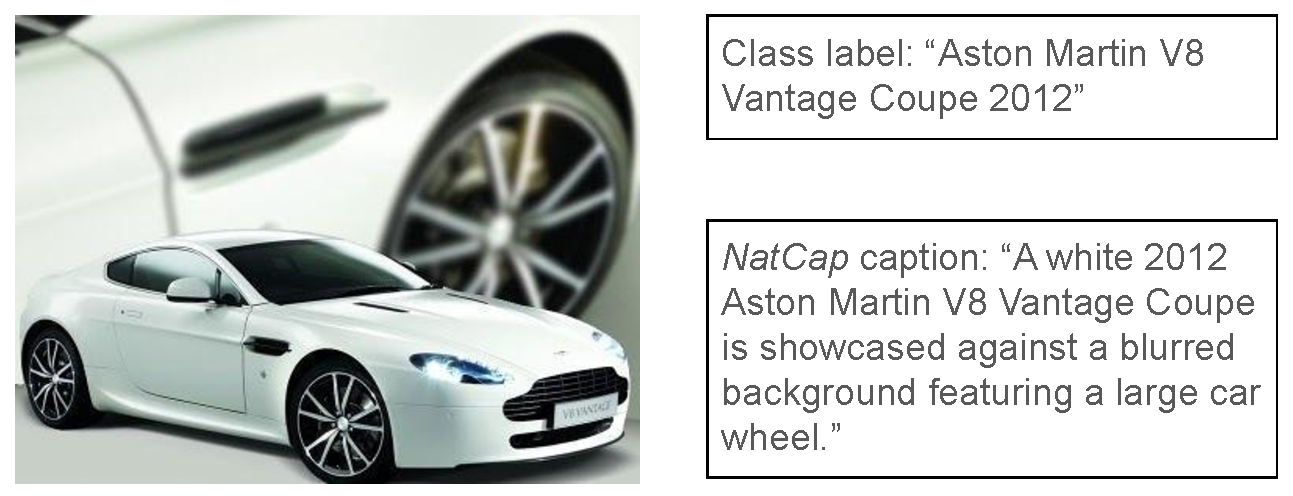
\includegraphics[width=0.95\textwidth]{images/modernvbert_figures/appendix/natcap_example.pdf}
    \caption[NatCap example]{Example from the NatCap dataset}
    \label{fig:natcap_example}
\end{figure}

\subsubsection{Contrastive Training Mix}
\label{appendix:contrastive_mix}

In this subsection, we describe the composition of our data mixes used in the contrastive training stages. \autoref{tab:cl_mix} outlines the datasets included in each mix, including the Document-Focused variant employed for \colflagship{}.
% \begin{table*}[t]
% \small
% \setlength{\tabcolsep}{6pt}
% \renewcommand{\arraystretch}{1.15}
% \begin{tabularx}{\textwidth}{l l X S[table-format=6.0] l}
% \toprule
% \textbf{Dataset} & \textbf{Source} & \textbf{Description} & {\textbf{\# Items}} & \textbf{Lang.} \\
% \midrule
% \multicolumn{5}{l}{\textit{ColPali train set}} \\
% & DocVQA                   & Document visual question answering.                                              & 39463  & English \\
% & InfoVQA                  & Infographic visual question answering.                                           & 10074  & English \\
% & TATDQA                   & Table-based QA from documents.                                                   & 13251  & English \\
% & arXivQA                  & QA over arXiv papers.                                                            & 10000  & English \\
% & Scraped docs (mixed)     & Broad, web-scraped documents across many topics.                                  & 45940  & English \\
% & \textbf{TOTAL}           &                                                                                   & \textbf{119000} \\
% \addlinespace[2pt]
% \midrule
% \multicolumn{5}{l}{\textit{Natural image retrieving - MSCOCO}} \\
% & MSCOCO Train Set (2017)   & Natural images and captions human crafted.                                                            & 118000  & English \\
% & \textbf{TOTAL}                                       & & \textbf{118000} \\
% \addlinespace[2pt]
% \midrule
% \multicolumn{5}{l}{\textit{Natural image captioning (Natcap)}} \\
% & caltech101  & General objects.                                                                  & 3000   & English \\
% & caltech256  & General objects.                                                                  & 30000  & English \\
% & cars        & Car model classification.                                                         & 8000   & English \\
% & country211  & Country where the picture is taken.                                               & 28000  & English \\
% & dtd         & Describable textures (texture attributes).                                        & 4000   & English \\
% & eurosat     & Land use / area zone type.                                                        & 16000  & English \\
% & fer2013     & Facial emotion recognition.                                                       & 28000  & English \\
% & fgcv\_aircraft & Aircraft model recognition.                                                     & 3000   & English \\
% & food101     & Food categories.                                                                  & 75000  & English \\
% & pets        & Dog/cat species.                                                                  & 3000   & English \\
% & resisc45    & Aerial scene / area zone type.                                                    & 18000  & English \\
% & sun397      & General scenes.                                                                   & 109000 & English \\
% & voc2007     & General objects.                                                                  & 8000   & English \\
% & \textbf{TOTAL}                                         & & \textbf{333000} & English \\
% \addlinespace[2pt]
% \midrule
% \multicolumn{5}{l}{\textit{Text retrieving (680K splits)}} \\
% & arguana                  & Argument retrieval.                                                               & 4065   & English \\
% & fever                    & Fact verification evidence retrieval.                                             & 28755  & English \\
% & fiqa                     & Financial QA.                                                                     & 5500   & English \\
% & hotpotqa                 & Multi-hop QA.                                                                     & 84516  & English \\
% & msmarco\_passage         & Web passage retrieval (MS MARCO).                                                 & 485823 & English \\
% & nq                       & Natural Questions.                                                                & 58568  & English \\
% & scidocsrr                & Scientific document relatedness ranking.                                          & 12654  & English \\
% & \textbf{TOTAL}&                                                                                   & \textbf{680000} & English \\
% \midrule
% \textbf{TOTAL}       &  &  & \textbf{1200000} & \\
% \bottomrule
% \end{tabularx}
% \caption{Sources and sizes used across domains. “\# Items” counts refer to query–page pairs, pages, images, or pairs as appropriate per row. \paul{TODO: remove lang column - it's ok I think, leave it}}
% \label{tab:cl_mix}
% \end{table*}

\begin{table}[ht]
\centering
\setlength{\tabcolsep}{4pt}
\renewcommand{\arraystretch}{1.15}
\begin{tabular}{l p{7cm} r c}
\toprule
\textbf{Source} & \textbf{Description} & \textbf{Pairs} & \textbf{Epochs} \\
\midrule
\multicolumn{4}{l}{\textbf{Generalist Mix}} \\
ColPali~\cite{faysse2025colpaliefficientdocumentretrieval} & Query–Document images for visual retrieval & 118k & 1 \\
MSCOCO~\cite{lin_microsoft_2014} & Natural images with human-written captions & 118k & 1 \\
\natcap~\textit{(ours, subsampled)} & Diverse images with synthetic captions & 118k & 1 \\
RLHN~\cite{thakur2025rlhn} & Text–text pairs for complex retrieval & 680k & 1 \\
\midrule
\textbf{TOTAL} & & \textbf{1030k} & \\
\midrule
\multicolumn{4}{l}{\textbf{Document-Focused Mix}} \\
ColPali~\cite{faysse2025colpaliefficientdocumentretrieval} & Query–Document images for visual retrieval & 118k & 3 \\
RLHN~\cite{thakur2025rlhn} & Text–text pairs for complex retrieval & 300k & 3 \\
\midrule
\textbf{TOTAL} & & \textbf{1254k} & \\
\bottomrule
\end{tabular}
\caption[Data mixes for contrastive training]{\textbf{Data mixes for contrastive trainings.} The \textit{Generalist Mix} spans over 1M diverse pairs, while the \textit{Document-Focused Mix} emphasizes document retrieval with extra ColPali epochs.}
\label{tab:cl_mix}
\end{table}



\section{Baselines Details}
\label{appendix:baselines}
In this section, we describe the models evaluated in as comparison to our document retriever model.

\noindent{\textbf{MoCa-3B}~\sidecite{chen2025mocamodalityawarecontinualpretraining}.} 
A modality-aware continual pretraining model that transforms a causal vision-language model into a bidirectional multimodal embedding model, using interleaved image-text reconstruction and contrastive alignment to support cross-modal retrieval.

\noindent{\textbf{GME-Qwen2}~\sidecite{zhang2025gmeimprovinguniversalmultimodal}.} 
A unified multimodal embedder built on Qwen2-VL~\sidecite{wang2024qwen2vlenhancingvisionlanguagemodels}, which produces shared embedding representations across text, image, and fused input modalities, enabling universal multimodal retrieval.

\noindent{\textbf{VLM2Vec}~\sidecite{jiang2024vlm2vectrainingvisionlanguagemodels}.} 
A method that trains a vision-language encoder by converting a VLM through extensive contrastive post-training. Flagship model is based on the model Phi-3.5~\sidecite{abdin_phi-3_2024}.

\noindent{\textbf{E5-V}~\sidecite{jiang2024e5vuniversalembeddingsmultimodal}.} 
An adaptation of the E5 embedding approach to multimodal models: it trains only on text pairs yet bridges the modality gap to handle image inputs, reducing cost while achieving universal embeddings.

\noindent{\textbf{ColPali}~\sidecite{faysse2025colpaliefficientdocumentretrieval}.} 
A vision-based document retrieval model that processes document pages as images (no OCR) and produces multi-vector embeddings via a late-interaction mechanism over PaliGemma~\sidecite{beyer2024paligemmaversatile3bvlm}, enabling efficient and accurate retrieval.

\noindent{\textbf{ColQwen2.5}~\sidecite{faysse2025colpaliefficientdocumentretrieval}.} 
An extension of ColPali~\sidecite{faysse2025colpaliefficientdocumentretrieval} using Qwen2-VL~\sidecite{wang2024qwen2vlenhancingvisionlanguagemodels} as the backbone, carrying forward the late interaction retrieval paradigm over page image embeddings, capturing layout and textual context without OCR.

\noindent{\textbf{Jina-v4}~\sidecite{günther2025jinaembeddingsv4universalembeddingsmultimodal}.} 
A multimodal embedding model combining visual and textual inputs with support for multi-vector (late interaction) embeddings, using adapters over a unified backbone to excel on visually rich document retrieval.

\noindent{\textbf{NemoRetriever}~\sidecite{xu2025llamanemoretrievercolembedtopperforming}.} 
An LI retriever that combines vision-language embeddings with a ColEmbed design, enabling high performance on visual document retrieval with structured patch matching and efficient similarity.

\noindent{\textbf{Jina CLIP}~\sidecite{koukounas_jina_2024}.} 
A smaller scale vision-language model using CLIP embeddings, applied to document retrieval tasks; although not LI, it offers a lightweight multimodal baseline.

\noindent{\textbf{BGE Visualized M3}~\sidecite{zhou2024vistavisualizedtextembedding}.} 
A vision-enhanced version of BGE M3~\sidecite{chen_bge_2024} that supports visual inputs and extends embedding models into multimodal domains.

\noindent{\textbf{SigLIP2-L-512/16}~\sidecite{tschannen2025siglip2multilingualvisionlanguage}.} 
A multilingual vision-language bi-encoder model, which combines image and text modalities to yield unified embeddings across languages. This configuration handles images of 512x512 pixels and create subpatches of 16x16 pixels.

\noindent{\textbf{ColFlor}~\sidecite{masrycolflor}.} 
A lightweight OCR-free visual document retriever with only 174M parameters built over Florence-2 and DaViT, delivering strong performance near ColPali with much lower computational cost and much faster encoding.


% \noindent{\textbf{colSmol-256M}.} 
% A scaled-down LI variant in the Col family at 256M parameters, intended to test retrieval efficacy in very low-resource regimes.

% \noindent{\textbf{colSmol-500M}.} 
% A moderate-size variant in the Col family at 500M parameters, serving as a mid-point benchmark in the efficiency



% \section{Model Architecture}
% \paul{Architectural details}
% \subsection{Pixel Shuffling.}
% \paul{appendix to explain compression ratio tradeoff} 
% \begin{figure}[t]
%     \centering
%     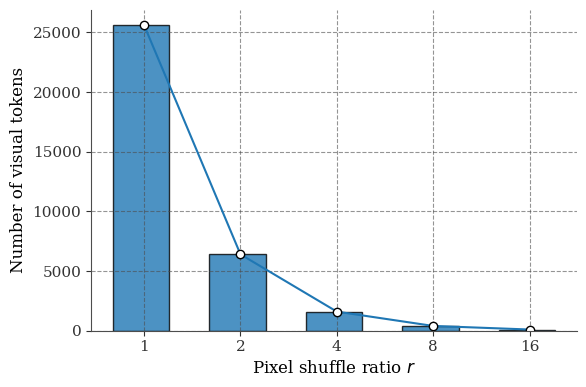
\includegraphics[width=0.7\textwidth]{images/modernvbert_figures/pixel_shuffling.png} % adjust width and filename
%     \caption{Empty caption}
%     \label{fig:pixel_shuffling}
% \end{figure}


\section{Additional Ablations}

\subsection{Performance Against Off-the-Shelf Dual Encoder}
\label{appendix:objective_downstream}
\textcolor{red}{We study whether using \textit{off-the-shelf} performances of the standalone vision tower are not outweighing the burden of adding language parameters and re-training through language modeling, as proposed in our work. Figure~\ref{fig:objective_downstream_noft} shows the results of the various models on the tasks described in Section~\ref{sec:methodology}. Similarly to Section~\ref{sec:ablation_tasks}, we observe that the early fusion model trained with LM objective significantly outperform the standalone vision tower on document retrieval tasks (+10.9 nDCG@5). It even surpass the larger dual encoder (+4.8 nDCG@5) on these latest tasks. We note that the standalone vision tower largely outperform the early fusion models on the other natural images tasks, supporting for the use of the SigLIP model for these tasks as found in various general benchmarks~\sidecite{xiao2025miebmassiveimageembedding}.}
\begin{figure}
    \centering
    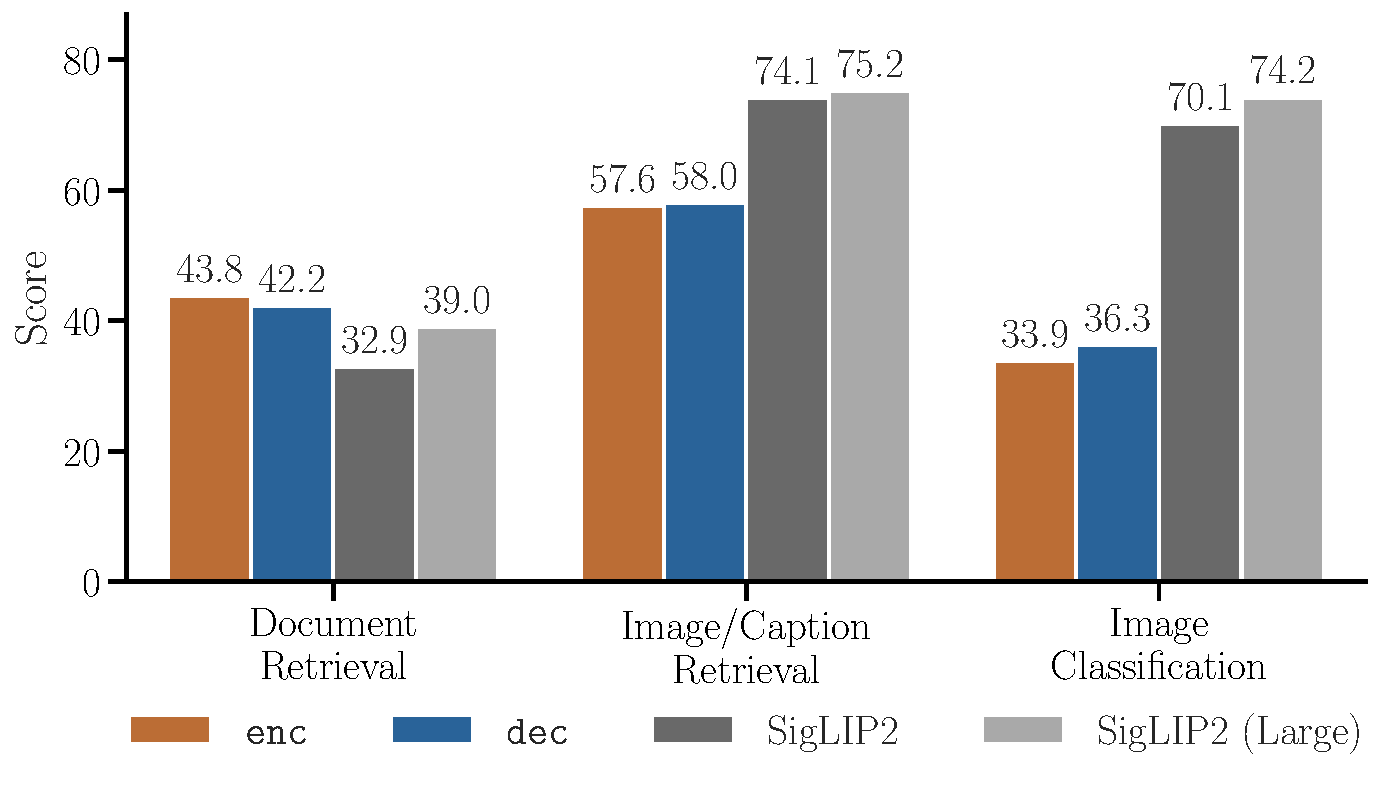
\includegraphics[width=0.75\linewidth]{images/modernvbert_figures/vbert_style/objective_downstream__rebuttal.pdf}
    \caption[Modality alignment impact]{\textbf{Impact of Modality Alignment objective on downstream tasks.} Early Fusion of vision and text models boosts document retrieval tasks regardless of the LM objective, but degrades natural image and classification tasks w.r.t. the standalone \textit{off-the-shelf} vision model SigLIP. Reported scores are aggregated MIEB scores (nDCG, Accuracy.)}
    \label{fig:objective_downstream_noft}
\end{figure}

\subsection{Scaling Dynamics of Attention Masks}
\label{appendix:mlm_vs_clm_scaling}
We study the different training dynamics of the different training objectives. We compare the \texttt{enc} (MLM) approach with a traditional \texttt{dec} (CLM) objective. Figure~\ref{fig:pt_scaling_clmvmlm} presents the performance of the two training objectives across a diverse set of tasks. While starting \texttt{dec} offers an advantage in low-data regimes, \texttt{enc} seems to catches up. In document retrieval tasks, it eventually surpasses \texttt{dec} and scales better.
\begin{figure}[ht]
    \centering
    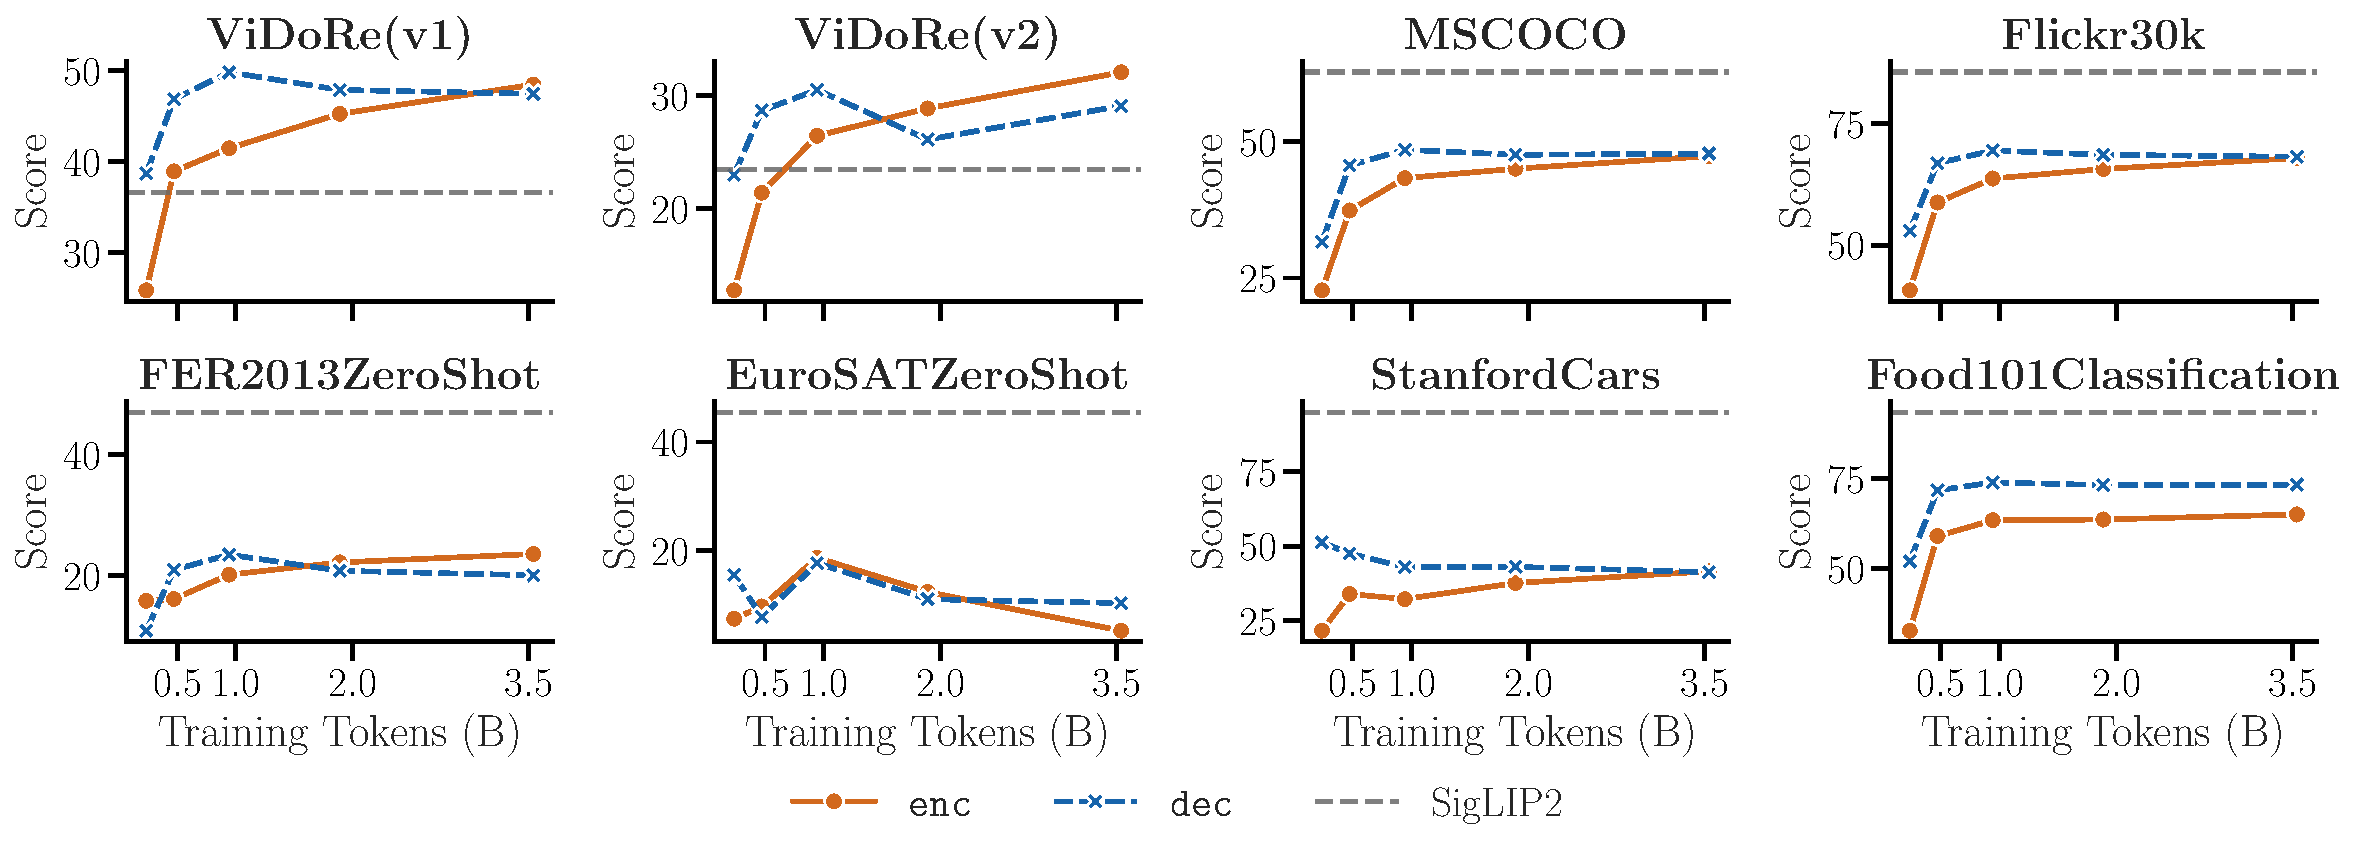
\includegraphics[width=\linewidth]{images/modernvbert_figures/appendix/pt_scaling_with_clm_all.pdf}
    \caption[Attention mask scaling impact]{\textbf{Attention masks impact on modality alignment phase scaling.} The dashed line marks the vision tower baseline. The orange curve shows the model initialized from a decoder LM with a \textit{CLM} objective, and the blue curve shows the model trained with an \textit{MLM} objective from an encoder LM. CLM performs better in low-data regimes, but MLM scales more effectively, surpassing CLM in document retrieval, while captioning and classification remain below the CLIP baseline.}
    \label{fig:pt_scaling_clmvmlm}
\end{figure}

\subsection{Bridging the Gap with Longer Contrastive Training}
\label{appendix:cl_scaling}
We study the impact of additional in-distribution training pairs on embedding tasks by scaling the contrastive training stage. Starting from the final checkpoint of our encoder-based ablation model, we double the contrastive dataset size at each step and train until convergence\sidenote{To avoid overfitting, we set an early stopping on an eval set. We limit the number of step to one epoch on the full dataset.}. This setup tests whether scaling continues to improve performance. 
Figure~\ref{fig:cl_scaling} shows the scaling behavior. Performance improves overall with more in-distribution data. The vision-tower baseline is quickly surpassed on visual document benchmarks, and scaling narrows the gap on other tasks\sidenote{Note that the models probably won't fully recover baseline vision-tower performance. This highlights the need to choose models according to use case (e.g., lightweight CLIP-like models for image classification).}. We note a plateau in captioning and classification, pointing to the need for more diverse data.  
\begin{figure}[ht]
    \centering
    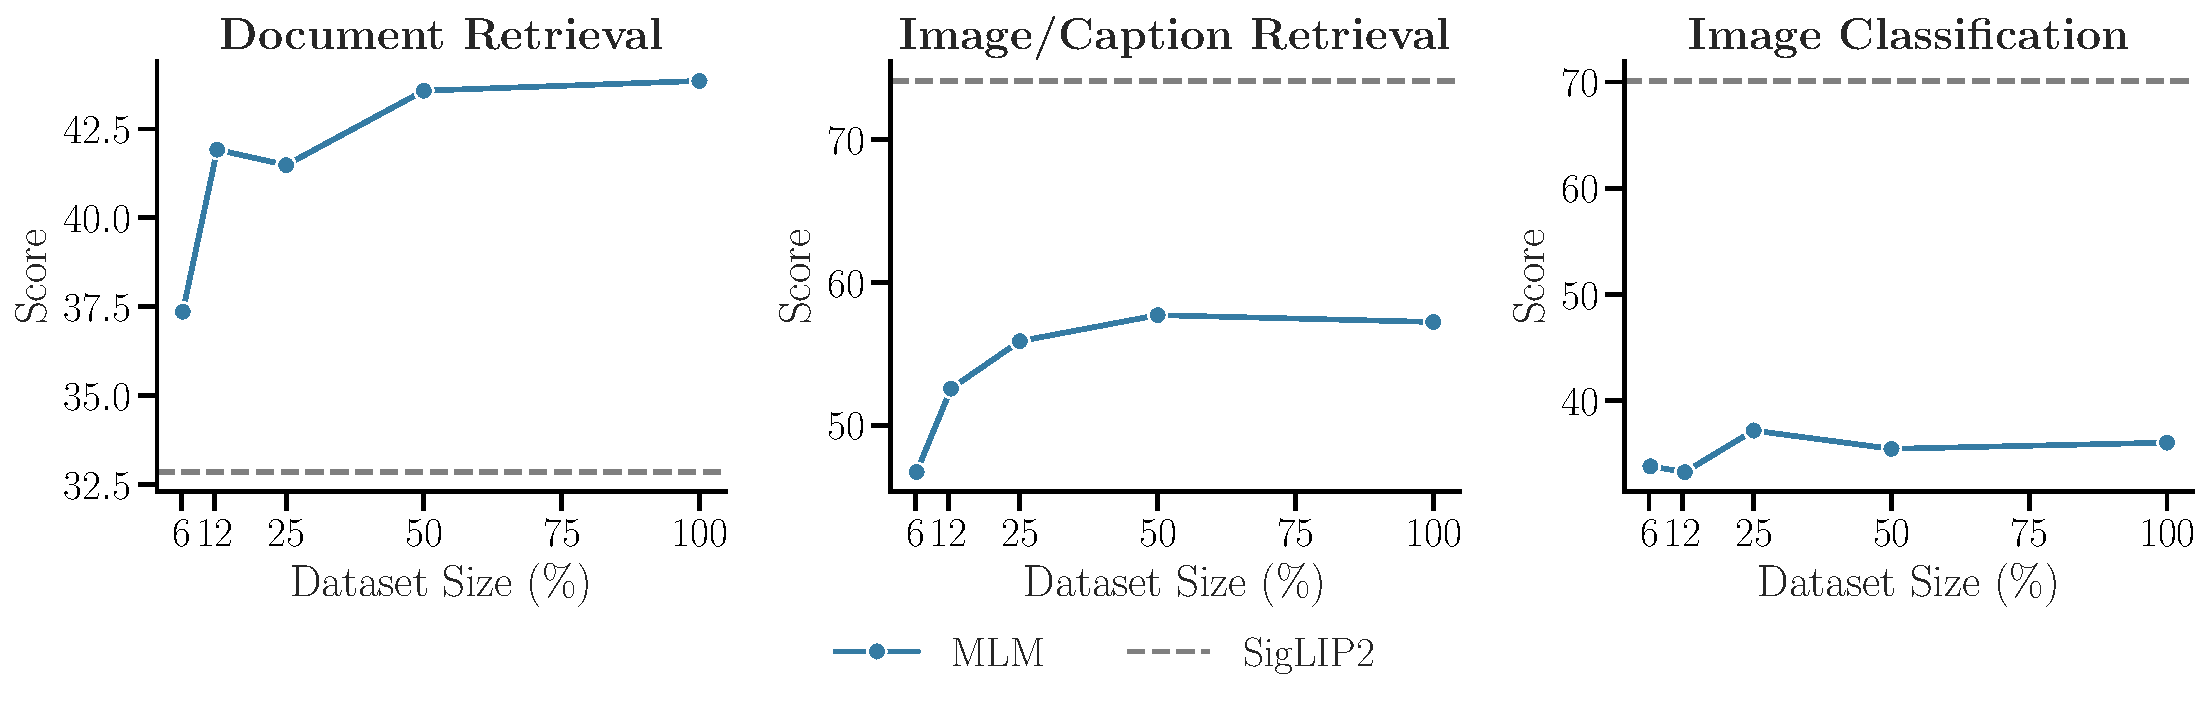
\includegraphics[width=\linewidth]{images/modernvbert_figures/vbert_style/cl_scaling.pdf}
    \caption[Contrastive training scaling]{Contrastive training scaling. Each dot on the blue curve represents one fraction of the baseline contrastive training mix (ColPali + MSCOCO). Performance improves with more in-distribution data, surpassing the baseline on document benchmarks and narrowing the gap on image captioning. There is no clear improvement in image classification, highlighting the need for more diverse pairs.}
    \label{fig:cl_scaling}
\end{figure}

\subsubsection{Optimal Text-To-Image Ratio for Document Retrieval}
\label{appendix:text_image_ratio}
Our findings in subsection~\ref{sec:scaling=-cont} indicate that incorporating additional text-only pairs boosts document retrieval performance. While our initial experiment employed a 1:1 text-to-image ratio, we further investigate how varying this ratio impacts our broad set of tasks. We start from the best contrastive mix in Table~\ref{table:cl_mix_impact}, and vary the text-to-image ratio. As shown in Figure~\ref{fig:text_image_ratio}, increasing the number of text-only pairs \textit{for a fixed amount of image pairs} consistently enhances retrieval performance. However, for natural image classification tasks, adding more text does not appear to provide benefits.

\begin{figure}[ht]
    \centering
    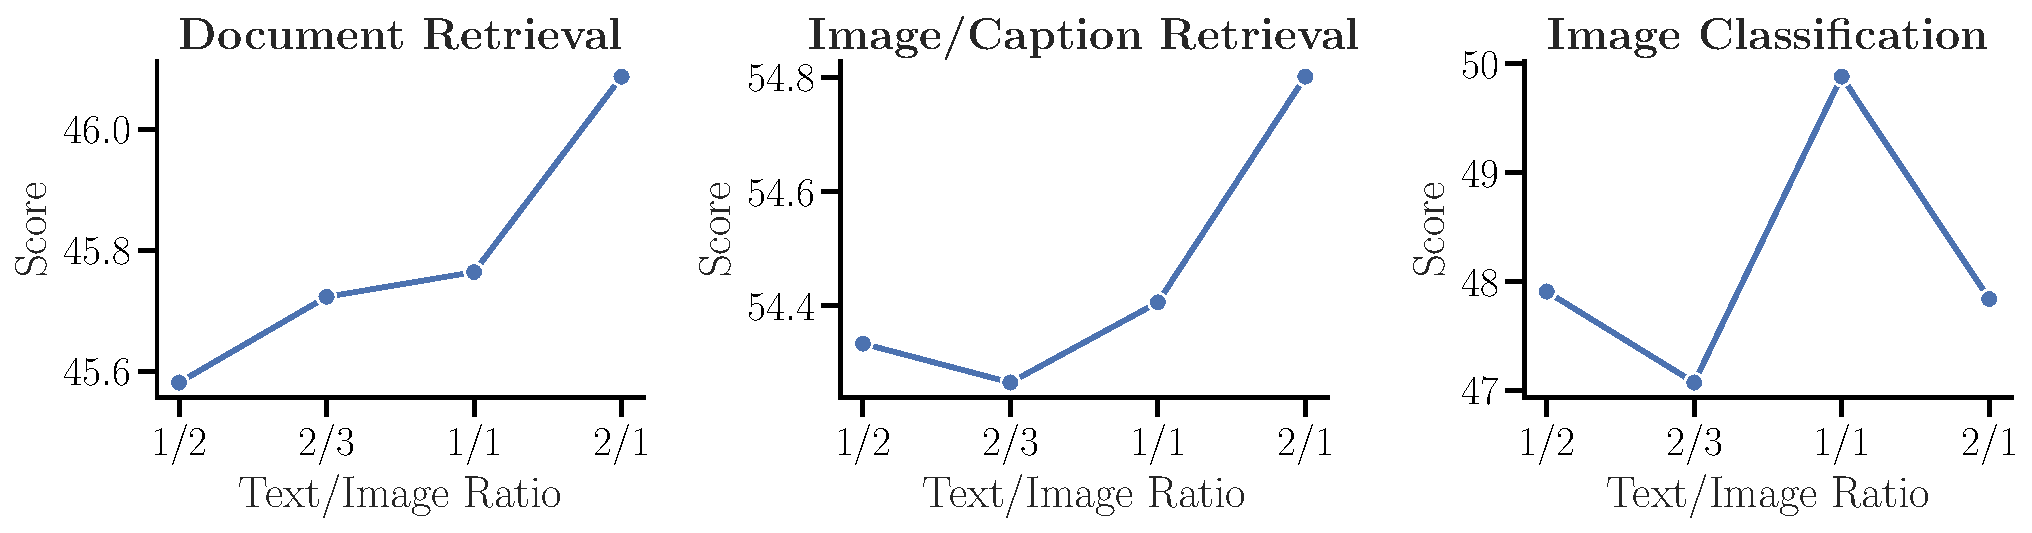
\includegraphics[width=.95\linewidth]{images/modernvbert_figures/appendix/image_text_ratio.pdf}
    \caption[Optimal text-to-image ratio]{\textbf{Optimal text-to-image ratio in contrastive training mix.} Increasing the ratio in retrieval tasks consistently improves the performances. }
    \label{fig:text_image_ratio}
\end{figure}

\subsection{Late Interaction for Non-Documental Retrieval}

\begin{table*}[ht]
  \centering
  \renewcommand{\arraystretch}{1.2}
  \small
  \resizebox{\textwidth}{!}{%
  \begin{tabular}{@{} >{}l c cccc >{\columncolor{avgcol}}c}
    & & \multicolumn{2}{>{\columncolor{grpA}}c}{\textbf{Document Retrieval}} & \multicolumn{2}{>{\columncolor{grpB}}c}{\textbf{Image/Caption Retrieval}} \\
    \cmidrule(lr){3-6}
& \rot{Model Size} & \rot{ViDoRe(v1)} & \rot{ViDoRe(v2)} & \rot{MSCOCO (T$\rightarrow$I)} & \rot{Flickr30k (T$\rightarrow$I)} & \rot{\textbf{Average}} \\

    \midrule
    \multicolumn{7}{@{}l}{\itshape CLIP Encoders}\\
    siglip2-base-patch16-512 & 376M & 36.6 & 23.4 & 66.2 & 86.9 & 53.3 \\
    siglip2-large-patch16-512 & 882M & 43.8 & 27.0 & 67.1 & 88.9 & 56.7 \\
    clip-vit-base-patch16 & 151M & 25.5 & 20.4 & 50.3 & 76.8 & 43.3 \\
    clip-vit-large-patch14 & 428M & 38.0 & 28.6 & 52.7 & 79.3 & 49.6 \\

    \midrule
    \multicolumn{7}{@{}l}{\itshape VLM-based Encoders}\\
    VLM2Vec-Full & 4150M & 49.8 & 36.5 & 59.5 & 81.8 & 56.9 \\
    % MoCa-Qwen25VL-3B & 3750M & 80.1 & 53.8 & 67.2 & 88.2 & 72.3 \\
    e5-v & 8360M & 62.7 & 49.4 & 68.1 & 89.8 & 67.5 \\

    \midrule
    \multicolumn{7}{@{}l}{\itshape Early Fusion Encoders}\\
    % blip-image-captioning-large & 470M & 0.8 & 0.8 & 0.1 & 0.0 & 0.4 \\
    bge-visualized-base & 196M & 10.3 & 9.0 & 50.0 & 74.1 & 35.9 \\
    bge-visualized-m3 & 873M & 12.4 & 10.2 & 39.6 & 69.0 & 32.8 \\
    \textbf{\flagshipembed{}} & 252M & 58.4 & 36.9 & 56.5 & 76.0 & 56.9 \\
    \textbf{\flagshipembed{} (multi-vector)} & 252M & 76.5 & 53.9 & 61.8 & 81.4 & \textbf{68.4} \\
    
    \bottomrule
  \end{tabular}%
  }
  \caption[Generalist retrieval performance]{\textbf{Generalist retrieval performances.} Late interaction benefits extend to non-documental retrieval tasks. Our multi-vector model increases its single-vector counterpart across all tasks, surpassing larger VLM-based retrievers. }
  \label{tab:results_generalist}
\end{table*}

We want to study if the multi-vector gains transfer to non-documental retrieval. To do so, we contrastively post-train our base model on our generalist post-training mix presented in Table~\ref{tab:cl_mix}.
The late interaction generalist exhibits superior performance in retrieval setting, improving its single-vector performance by +20.2\% (11.5 points), matching the performance of substantially larger VLM-based retrievers like E5-V (8.3B parameters, 67.5 points) and surpassing dual encoders like SigLIP (882M parameters, 56.7 points). This matches the capabilities observed in Section~\ref{sec:ablation_tasks} for documental settings for models with native bidirectional attention, extending it to natural image tasks. This result extends the prevailing understanding from the document retrieval community, where the superiority of late-interaction is well-documented (\cite{khattab_colbert_2020}, \cite{GTE-ModernColBERT}, \cite{faysse2025colpaliefficientdocumentretrieval}). While this performance gap is widely accepted for document retrieval, its applicability to caption matching tasks has not really been addressed. Our findings provide strong evidence that the fine-grained matching capabilities of late-interaction models are a key driver of performance in this domain too.


\subsubsection{Model Merging}\label{appendix:model_merging}
Our contrastive learning stage provides direct performance trade-offs on different tasks. Following recent trends, we evaluate how model merging techniques allow to mitigate performance degradation on specific tasks, while maintaining the performance enabled by the contrastive training \sidecite{sung2023empiricalstudymultimodalmodelmerging, dziadzio2024mergemultimodalmodelstime, li2024improvinggeneraltextembeddingmerging, zhang2025qwen3embeddingadvancingtext}. We merge our ablation model after modality alignment with the checkpoint after the full contrastive learning with two methods: SLERP \sidecite{ilharco2022patchingopenvocabularymodelsinterpolating} and average merging \sidecite{slerp_original}. For SLERP, we compare three values for the $\lambda$ coefficient ($0.25$, $0.5$, $0.75$). \autoref{fig:model_merging_results} displays the the trends with the best method (SLERP, $\lambda = 0.75$). As we can see, the merged model mitigates the performance drop in Image/Caption Retrieval tasks, while maintaining significant gains on Image Classification tasks. However, merging strongly degrades performance on Document Retrieval, showing that benefits of merging embedding models are task-dependent. 

\begin{figure}[ht]
    \centering
    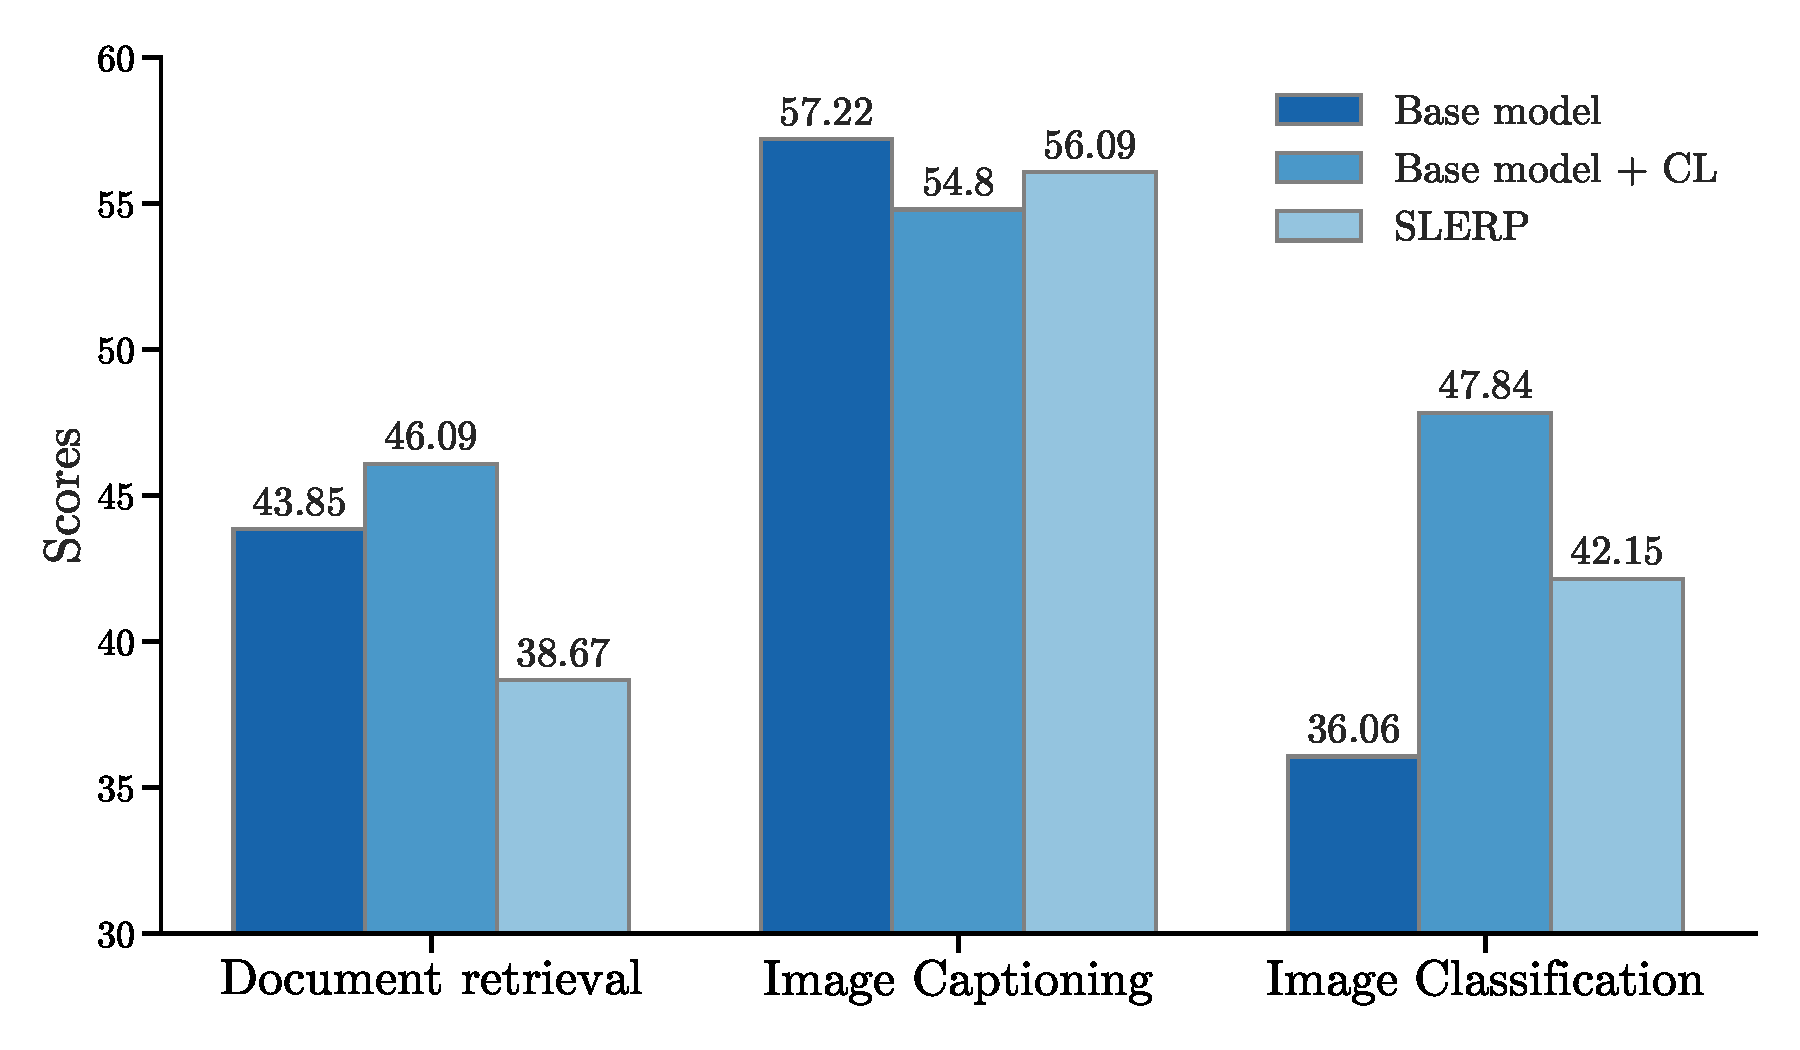
\includegraphics[width=.7\linewidth]{images/modernvbert_figures/appendix/grouped_model_performance2.pdf}
    \caption[Merging model results]{Merging model results across tasks. Benefits are task-dependent, with performance degradation w.r.t. both original models in Document Retrieval.}
    \label{fig:model_merging_results}
\end{figure}

% \subsubsection{Late Interaction for caption-image retrieval}
% Another finding of our work is that late-interaction models substantially improves over an equivalent dense encoder on caption-to-image retrieval. This result extends the prevailing understanding from the document retrieval community, where the superiority of late-interaction is well-documented (\cite{khattab_colbert_2020}, \cite{GTE-ModernColBERT}, \cite{faysse2025colpaliefficientdocumentretrieval}). While this performance gap is widely accepted for document retrieval, its applicability to caption matching tasks has not really been addressed. Our findings provide strong evidence that the fine-grained matching capabilities of late-interaction models are a key driver of performance in this domain too.


\subsubsection{Curriculum For Document Retriever Contrastive Post-Training}

\begin{table}{t}
% \vspace{-10pt}
\centering
\renewcommand{\arraystretch}{1.2}
\small
\resizebox{\linewidth}{!}{%
  % --- your tabular code unchanged ---
  \begin{tabular}{@{} l cc >{\columncolor{avgcol}}c}
    & \rot{ViDoRe(v1)} & \rot{ViDoRe(v2)} & \rot{\textbf{Average}} \\
    \toprule
    \multicolumn{4}{@{}l}{\itshape Document retrieval contrastive training starting checkpoint}\\
    \midrule
    \flagship{}-base                        & \textbf{81.2} & \textbf{56.0} & \textbf{68.6} \\
    \hspace{1cm} + multi-vector generalist CL  & 80.7 & 55.4 & 68.1 \\
    \hspace{1cm} + single-vector generalist CL   & 80.6 & 54.0 & 67.3 \\
    \bottomrule
  \end{tabular}
}
\caption[\flagship{} curriculum performance]{\textbf{Performance of \flagship{} Document Specialisation Curriculums.} This table presents the performance of various contrastive training curriculums starting from \flagship{}-base, on the ViDoRe(v1) and ViDoRe(v2) benchmarks. The generalist contrastive learning mix used in the last two models is detailed in Table~\ref{tab:cl_mix}. We see that a preliminary stage of generalist contrastive learning harms the final document retrieval performance, regardless of whether a multi-vector approach is used.}
\label{appendix:flagship_ablations}
\end{table}


We conduct an ablation study to determine the optimal contrastive training curriculum for specializing \flagship{} in document retrieval. Specifically, we investigate whether a preliminary generalist contrastive training phase, intended to leverage a larger dataset, improves downstream performance. As shown in Table \ref{appendix:flagship_ablations}, our results demonstrate that this initial generalist phase is detrimental to final performance ($-0.5\%$). The optimal strategy is to specialize the model on the target task directly after its initial Masked Language Modeling (MLM) alignment.

\subsection{Text-Only Retrieval}
\begin{table}[h]
\centering
\begin{tabular}{l r r}
  \toprule
  Model & Params (M) & NDCG@5 \\
  \midrule
  \multicolumn{3}{l}{\textbf{Statistical}} \\
  BM25s & — & 0.559 \\
  \midrule
  \multicolumn{3}{l}{\textbf{Single Vector}} \\
  Jina Embeddings v4 & 3577* & 0.623 \\
  E5-large-v2 & 335 & 0.605 \\
  bge-m3 (Bi Encoder) & 567 & 0.590 \\
  Qwen3-Embedding-0.6B & 600 & 0.567 \\
  % \biflagship{} & 150* & 0.429 \\
  \midrule
  \multicolumn{3}{l}{\textbf{Multi Vector}} \\
  LightOn GTE-ModernColBERT v1 & 149 & 0.669 \\
  Jina ColBERT v2 & 137 & 0.642 \\
  bge-m3 (Late Interaction) & 567 & 0.606 \\
  ColBERT v2 & 110 & 0.593 \\
  Colqwen2-v1.0 & 1580* & 0.593\\
  \colflagship{} & 150* & 0.589 \\
  Colqwen2.5-v0.2 & 3145* & 0.589\\
  \bottomrule
\end{tabular}
\caption[NanoBEIR performance]{Average NDCG@5 of \colflagship{} on NanoBEIR, a text retrieval benchmark with multiple sub domains. *For multimodal models, we only consider parameters of the text encoder}
\label{appendix:text_perf}
\end{table}

The results in Table \ref{appendix:text_perf} detail the performance of \colflagship{} and other baselines on the NanoBEIR text retrieval benchmark. It achieves an average NDCG@5 score competitive with single and multi vector models specialized for text, even without explicit optimization for this modality. This performance is encouraging and indicates a promising direction for training a unified model for both text and image retrieval.

\subsection{Model Latency}

\subsubsection{Image Resolution Tradeoffs}
\label{appendix:visual_tokens}

\textcolor{red}{Figure~\ref{fig:tokens_shuffling_tradeoff} presents the pixel shuffling trade-off. Processing larger images creates more visual tokens, leading to very long sequences (around $17'500$ tokens for a 2048x2048 px image with no pixel shuffling). Pixel shuffling allow to compress these sequence by concatenating the embeddings of spatially close patches. This diminishes the number of tokens for longer visual token embeddings. Table~\ref{tab:image_resolution_latency} presents the latency to process one image of various resolutions on one L4 GPU and CPU.}

\begin{figure}[ht] 
\centering 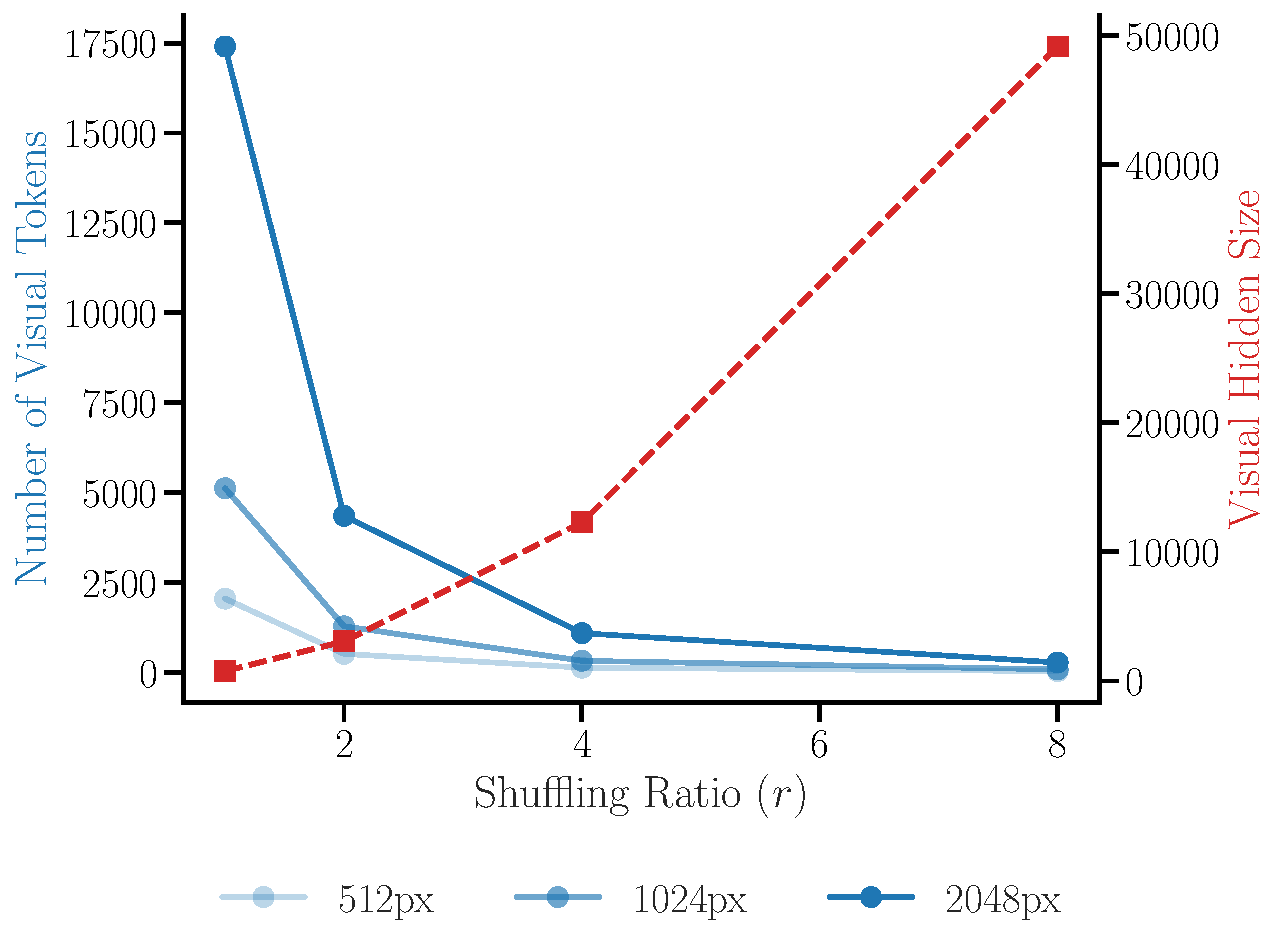
\includegraphics[width=0.6\linewidth]{images/modernvbert_figures/visual_tokens_hidden_size_vs_shuffling_ratio.pdf} 
\caption[Image processing parameters impact]{\textbf{\textcolor{red}{Image processing parameters impact on visual tokens.}} Here we assume a square image for simplicity. Scaling the image size introduces naturally more tokens, but having a large enough pixel shuffling ratio ($r\geq4$) allows to counterbalance by concatenating spatially close patch representations.} \label{fig:tokens_shuffling_tradeoff} \end{figure}

\begin{table}[ht]
    \centering
    \renewcommand{\arraystretch}{1.0}
    \small
    \resizebox{0.85\textwidth}{!}{%
    \begin{tabular}{@{} l c cc}
    & {\textbf{Num. Visual Tokens}} & {\textbf{CPU Latency (ms)}} & {\textbf{GPU Latency (ms)}} \\
    
    \midrule
    $512$px & $128$ & $287.2_{(\pm 7.8)}$ & $43.6 _{(\pm 1.4)}$ \\
    $1024$px & $320$ & $1015.8 _{(\pm 58.1)}$ & $150.3 _{(\pm 2.5)}$ \\
    $2048$px & $1088$ & $2572.0 _{(\pm 63.9)}$ & $363.4 _{(\pm 4.6)}$ \\
    
    \bottomrule
    \end{tabular}%
    }
    \caption[\flagship{} image processing latency]{\textcolor{red}{\textbf{\flagship{} image processing latency}}. Computing the average time to process a single image on GPU and CPU. The average is computed on 100 images. The values represent the mean latency in milliseconds, with the standard deviation included in parenthesis.}
    \label{tab:image_resolution_latency}
\end{table}

\subsubsection{Online Query Encoding Latency}
\label{appendix:gpu_latency}
\textcolor{red}{We evaluate the query embedding speed of our model on GPU. We use a single Nvidia H100 with 80GB of VRAM. As for Section~\ref{sec:results}, latencies are computed in batch size 1 to simulate online situations, and are averaged over all NanoBEIR queries. Only the text parameters are loaded and run, to minimize memory usage. Parameters are cast to bfloat16 and Flash Attention 2 is used. The resulting speeds are often much faster than those obtained by running inference through each model's reference implementation. Results are shown in Table~\ref{table:pu_latency}). Interestingly in this setup where memory is not a bottleneck, model depth seems to be a large performance driver, sometimes more the parameter count.
We finally evaluate batched GPU throughput. We use batches of size 512 by default and iteratively half it when memory is insufficient. We observe that \flagship{} based models are extremely fast and can process 5000 queries per second. In the table, the reported figures correspond to the inverted throughput (latency per batch divided by the number of queries per batch). These speed and throughput gains are made possible due to a combination of size, and efficient hardware-informed design as well as the support of flash attention and sequence packing other models of the size often lack \sidecite{warner2024smarterbetterfasterlonger}.
}




\begin{table*}[t]
  \centering
  \renewcommand{\arraystretch}{1.03}
  \small
  \resizebox{\textwidth}{!}{%
  \begin{tabular}{@{} >{}l c c >{\columncolor{latcpucol}}c >{\columncolor{latgpucol}}c >{\columncolor{latcpucol}}c}
    & {Late Interaction} & {Model Size (B)} &
      \rot{\textbf{CPU Latency (ms)} \hspace{5pt}} & \rot{\textbf{GPU Latency (ms)}} & \rot{\textbf{GPU Batching (ms)}} \\

    \midrule
    \multicolumn{6}{@{}l}{\itshape $\ge$ 1B Parameters}\\

    MoCa-3B &  & 3.75 &
      $158_{(\pm 147)}$ & $26_{(\pm 3)}$ & $4.54$ \\

    VLM2Vec &  & 4.15 &
      $211_{(\pm 253)}$ & $21_{(\pm 3)}$ & $2.82$\\

    GME-Qwen2-7B &  & 8.29 &
      $412_{(\pm 411)}$ & $25_{(\pm 1)}$ & $9.07$\\

    E5-V &  & 8.36 &
      $434_{(\pm 379)}$ & $22_{(\pm 2)}$ & $9.55$\\

    ColPali & \cmark & 2.92 &
      $175_{(\pm 113)}$ & $14_{(\pm 1)}$& $3.07$ \\

    ColQwen2.5 & \cmark & 3.75 &
      $158_{(\pm 147)}$ & $26_{(\pm 2)}$ & $26$\\

    Jina-v4 & \cmark & 3.75 &
      $158_{(\pm 147)}$ & $26_{(\pm 2)}$ & $4.54$\\

    NemoRetriever-3B & \cmark & 4.40 &
      $155_{(\pm 118)}$ & $20_{(\pm 2)}$ & $4.59$ \\

    \midrule
    \multicolumn{5}{@{}l}{\itshape $\le$ 1B Parameters}\\

    Jina CLIP &  & .22 &
      $14_{(\pm 7)}$ & $6_{(\pm 2)}$ & $.69$\\

    BGE Visualized M3 &  & .87 &
      $38_{(\pm 42)}$ & $10_{(\pm 2)}$ & $.77$ \\

    SigLIP2-L-512/16 &  & .88 &
      $25_{(\pm 8)}$ & $6_{(\pm 1)}$ & $.10$\\

    ColFlor & \cmark & .17 &
      $17_{(\pm 9)}$ & $8_{(\pm 2)}$ & $.31$\\

    \biflagship{} (ours) &  & .25 &
      $20_{(\pm 11)}$ & $14_{(\pm 2)}$ & $.20$\\

    \textbf{\colflagship{} (ours)} & \cmark & .25 &
      $20_{(\pm 11)}$ & $14_{(\pm 2)}$ & $.20$\\

    \bottomrule
  \end{tabular}%
  }
  \caption[Text query encoding latency]{\textcolor{red}{\textbf{Text query encoding latency.}} The latency is computed both on high-end CPUs (1TB RAM, 128 cores) and GPU (Nvidia H100, 80GB) (mean ± std). Since only 649 queries are used, standard deviations are not reported in GPU batching mode (batches of 512 queries by default), for which we report the inverse throughput (average latency per batch divided by the batch size).}
  \label{table:pu_latency}
\end{table*}


% buggy layout, this has to be on seperated page
\clearpage
\begin{tcolorbox}[colback=gray!5,colframe=black,title=\natcap{} Annotation Prompt,fonttitle=\bfseries]
You are an image annotator expert.\\\\
You will receive an image along with its classification label and the classification task scope, and your task is to provide contextualized metadata about it.\\\\
The output should be a JSON object with the following metadata fields:
\begin{itemize}
  \item \textbf{caption}: A descriptive caption of the image accounting for its label. This should be a \textbf{unique} and concise sentence that describes the image in detail.
  \item \textbf{class\_tags}: A list of tags that represents the image and can help identify the class. (e.g., for a car image with its model as a class, this could be some specific attribute of the car)
  \item \textbf{other\_tags}: A list of tags that represents the image but can help identify the image among others of the same class. (e.g., for a car image with its model as a class, this could be its color or the background of the image)
  \item \textbf{is\_image\_class\_explicit}: Boolean, could the class be inferred from the image alone? (e.g., the class is a country and you cannot necessarily infer it from the image alone, so this would be \texttt{false})
\end{itemize}

Please ensure that the output is in valid JSON format.\\

\textbf{Example:}\\
You receive an image of what is clearly a car with its model as a class (here Audi TTS coupe 2012) for a car model classification task.\\
The output could be a JSON object like this:

\begin{lstlisting}[basicstyle=\ttfamily\small]
{
  "caption": "A red Audi TTS coupe 2012 car parked on a sunny street 
                in front of a sport shop.",
  "class_tags": ["sport coupe","four door coupe","17'' alloy wheels"],
  "other_tags": ["sunny street","parked","red","sport shop"],
  "is_image_class_explicit": true
}
\end{lstlisting}

\textbf{------}\\
Classification scope: \{task\_info\}\\
Image label: \{label\}\\
Answer:
\label{box:natcap_prompt}
\end{tcolorbox}

% 
\section{\textit{ConTEB} Details}\label{app:conteb_stats}

% \begin{figure*}[htbp]
%   \centering
%   \includegraphics[width=\textwidth]{images/benchmark_creation_horizontal.pdf}
%   \caption{Benchmark creation process.}
%   \label{fig:benchmark_creation}
% \end{figure*}



This appendix describes the data generation process employed in this project. The methodology varies based on the dataset source, but generally, long documents are segmented into smaller chunks. If preexisting queries are available, they are mapped to relevant chunks using either provided answer spans (e.g., SQuAD) or tagged using GPT-4o. In cases where queries are unavailable, a large language model (LLM) generates them before associating them with the relevant text segments. This approach, illustrated in \ref{fig:benchmark_creation}, is systematically applied across multiple datasets.


\subsection{Wiki-based Datasets} \label{app:wiki-based}

\emph{Football} and Geography are our two wiki-based datasets, focusing on the Sports and Geography domains.

\noindent\textbf{Wikipedia Data Extraction}
The pipeline first retrieves Wikipedia summaries for a given person using the \texttt{wikipediaapi} library. The extracted summary is then split into paragraphs.

\noindent\textbf{Text Rephrasing}
Each paragraph from the Wikipedia summary undergoes a rephrasing process to remove direct mentions of the person’s name while maintaining the original context. The rephrased text replaces names with pronouns such as ‘he’ or ‘she’. This transformation is performed using the GPT-4o model via the following prompt:

\begin{quote}
\textit{
Here is a Wikipedia article:
\texttt{[Full Wikipedia Summary]}
Can you rephrase the following paragraph to remove all mention of the name of the person the article is about? You can leave other names as is and can replace the name with words such as 'he/she' or other generic paraphrases.
\texttt{[Paragraph to be rephrased]}
}
\end{quote}

\noindent\textbf{Question Generation}
For each paragraph in the summary, the model generates three questions related to the person. The questions explicitly mention the person's name but do not include other named entities such as dates or proper nouns. The generation follows this structured prompt:

\begin{quote}
\textit{
Here is a Wikipedia article:}

\texttt{[Full Wikipedia Summary]}

Using specifically the following paragraph, can you ask 3 questions related to the person the article is about? Each question must mention the name of the person, but the question should not contain other named entities (dates, other proper nouns). Format the response as a Python list of strings and do not output anything else.

\texttt{[Paragraph to be used for question generation]}

\end{quote}


\subsection{NarrativeQA, COVID-QA, MLDR}

\textit{NarrativeQA} (literature), \textit{MLDR} (encyclopedic) and \textit{Covid-QA} (medical) consist of long documents, associated to existing sets of question-answer pairs. 

We chunk these documents, and use GPT-4o to annotate which chunk, among the gold document, best contains information needed to answer the query. Since chunking is done \textit{a posteriori} without considering the questions, chunks are not always self-contained and eliciting document-wide context can help build meaningful representations. 

\textbf{Synthetic Query Generation:} To extend MLDR for our training dataset, OpenAI's GPT-4o model is prompted to generate 20-50 realistic queries per document, ensuring that each query aligns with the content of at least one chunk. This is on top of the queries that are already incuded in the dataset. Synthetic queries are included only in our training dataset.


\subsection{Insurance} 
\textit{Insurance} is composed of a long document with insurance-related statistics for each country of the European Union. Countries are often not referred to in-text, but only once in the section title. Therefore, certain chunks require knowledge of their position within the document to be properly disambiguated from others. Questions are manually crafted to require structural understanding for accurate chunk matching. This process, in addition to manual verification of the contextuality quality, makes \textit{Insurance} a controlled dataset. Since questions are crafted after the chunking process, the annotation results directly from the manual question generation process.

\subsection{SQuAD}

\textit{SQuAD} is an extractive QA dataset with questions associated to passages and annotated answer spans, that allow us to chunk individual passages into shorter sequences while preserving the original annotation.

\subsection{ESG Reports}

\textit{ESG Reports} contains long documents from the fast-food industry, with manually annotated query-page pairs from the ViDoRe Benchmark v2 \sidecite{macé2025vidorebenchmarkv2raising}, originally thought for visual retrieving\footnote{\url{https://huggingface.co/datasets/vidore/restaurant_esg_reports_beir}}. We convert all documents to text, chunk them, and re-annotate the resulting passages by hand, filtering out queries that relied solely on visual aspects (e.g., tables, graphs).


% \begin{table*}[h]
%     \centering
%     \small
%     \resizebox{\textwidth}{!}{
%     \begin{tabular}{lcccccc}
%     \toprule
%      & \# Positives (per query) & \# Docs & Tokens/Chunk & Chunks/Doc & Query generation & Chunk Annotation \\
%     \midrule
%     \textbf{In Domain} & \\
%     Chunked MLDR & 100 (1) & 100 & 170.5 & 15.4 & Synthetic & Synthetic \\
%     NarrativeQA & 8575 (1) & 355 & 154.5 & 4.9 & Human & Synthetic \\
%     SQuAD Chunked & 2067 (1) & 2067 & 19.1 & 8.5 & Human & Manual \\
%     \midrule
%     \textbf{Out-Of-Domain} & \\
%     \textcolor{navyblue}{\textbf{Footballers}} & 1767 (1) & 224 & 86.1 & 3.6 & Synthetic & Human in the loop \\
%     \textcolor{navyblue}{\textbf{Geography}} & 5283 (1) & 530 & 113.6 & 4.3 & Synthetic & Human in the loop \\
%     \textcolor{navyblue}{\textbf{Insurance}} & 120 (1) & 1 & 80.7 & 60 & Human & Manual \\
%     Covid-QA & 1111 (1) & 115 & 153.9 & 29.1 & Human & Synthetic \\
%     ESG Reports & 75 (2.3) & -- & -- & -- & Human & Manual \\
%     NanoBEIR* & 650 (1) & 4363.3 & 199.4 & 1 & Human & Manual \\
%     \bottomrule
%     \end{tabular}
%     }
%     \caption{Merged \emph{ConTEB} dataset details and statistics. Controlled datasets are highlighted in \textcolor{navyblue}{\textbf{bold blue}}. Values marked \texttt{--} indicate missing statistics in the source tables.}
%     \label{table:merged_conteb}
% \end{table*}


\subsection{Training Data Statistics}\label{app:training_data}

\autoref{table:training-data} displays information about the training data. Our refined version of MLDR forms a large part of the training corpus. We can see that the majority of chunks are used as positives at least once, ensuring that the model is not biased towards the position of the chunk in the sequence.

\begin{table}[ht]
    \centering
    % \renewcommand{\arraystretch}{1.2} % Adjust row spacing
    \resizebox{\linewidth}{!}{%
    \begin{tabular}{l|rrr|r}
    \toprule
     & MLDR & NarrativeQA & SQuAD & Total \\
    \midrule
    Number of Docs & 8467 & 972 & 442 & 9881 \\
    Number of Chunks & 213001 & 5219 & 14367 & 232587 \\
    Number of Queries & 211933 & 27953 & 67355 & 307241 \\
    Number of Chunks per Doc & 25.2 & 5.4 & 32.5 & 23.5 \\
    \% Chunks with associated Query & 94.6\% & 81.9\% & 100.0\% & 94.61\% \\
    Number of Tokens per Doc & 3962.6 & 819.1 & 4966.1 & 3698.2 \\
    Number of Tokens per Query & 16.7 & 21.9 & 12.5 & 16.3 \\
    \bottomrule
    
    \end{tabular}
    }
    
    \caption[Training dataset statistics]{Training Dataset Statistics} 
    \label{table:training-data}
\end{table}





%\section{Training Setup}\label{app:training_setup}

%We train all our models using a customized version of the \texttt{sentence-transformers} trainer \footnote{\url{https://sbert.net/docs/package_reference/sentence_transformer/trainer.html}}, using the PyTorch BF16  mixed precision on 4-GPU nodes. We use a cosine decay learning rate scheduler with a warm-up phase of 55 steps. Below are the model-specific parameters. All parameters that are not specified are set to the default values of the \texttt{sentence-transformers} trainer. The models are evaluated every 100 training steps.

%\subsection{ModernBERT base variants}
%We fine-tune \texttt{modernbert-embed-base} and \texttt{gte-modernbert-base} using a per-device batch size of 8 and a learning rate of $1e-4$.

%\subsection{ModernBERT large}
%We fine-tune \texttt{modernbert-embed-large} using a per-device batch size of 4 and a learning rate decreased accordingly to $5e-5$.

% \subsection{Prefix}


\section{Implementation Details}

\subsection{Sequence prefixes}

ModernBERT-based models are trained with query and document prefixes. We apply the same approach in our training and inference frameworks. After several tests, we opt for using a single document prefix for the Late Chunking sequence, instead of adding a document prefix at the beginning of each chunk inside the same sequence. We separate chunks with [SEP] tokens to let the model understand the concept of chunks during its token embedding computation.


\subsection{Late Interaction Models}

We leverage the \texttt{pylate} \sidecite{PyLate} library for the Late Interaction implementation. For training LI models with InSeNT, we adapt the LI mechanisms to incorporate it with Late Chunking in our own codebase. In particular, we do not use token skiplists at inference time, and use a single document prefix for the whole document sequence.

\section{Additional Results}
\label{app:res}

\subsection{Training with concatenated short documents}

Results of training an InSeNT model with concatenated short document data (using the Nomic dataset) are available in \autoref{table:nomic-results}. Short docs are clustered from the \texttt{nomic-supervised} dataset \cite{nussbaum2024nomic} following \sidecite{morris2024contextualdocumentembeddings}. This approach did not yield promising results, proving that natively long documents are necessary to induce relevant in-sequence signal.


\begin{table*}[ht]
    \centering
    \renewcommand{\arraystretch}{1.2} % Adjust row spacing
    \resizebox{\textwidth}{!}{%
    \begin{tabular}{l|rrr|rrrr|r|rr}
\toprule
     & MLDR & SQuAD & NarrativeQA & Football & Geography & COVID-QA & Insurance & NanoBEIR & Average & Runtime (s) \\
    \midrule
    MB & 78.4 & 73.4 & 77.9 & 19.1 & 56.2 & \textbf{61.7} & 12.4 & \textbf{63.2} & 55.3 & 40.0\\
    \midrule
    MB+InSeNT(Nomic) & 77.8 & 76.0 & 76.2 & 26.2 & 62.7 & 38.8 & 63.7 & 59.9 & 60.2 & 36.3\\
    MB+Late Chunking & 78.5 & 77.1 & 75.8 & 54.6 & 89.6 & 40.0 & 41.0 & \textbf{63.2} & 65.0 & 36.3 \\
    \textbf{Ours: MB+InSeNT} & \textbf{88.7} & \textbf{80.9} & \textbf{81.3} & \textbf{63.9} & \textbf{90.7} & 56.0 & \textbf{100.0} & 60.4 & \textbf{77.8} & 36.3 \\
    \bottomrule
    \end{tabular}}

    \caption[ConTEB evaluation results]{Evaluation (nDCG@10) of baseline models and our proposed method on \textit{ConTEB}. We show MB+InSeNT(Nomic) behaves like a non-contextual model after training on independant documents concatenated in a single sequence.} 
    \label{table:nomic-results}
\end{table*}

\subsection{Full ablation results on $\lambda_{seq}$}

We show the results of the different values for $\lambda_{seq}$ on all our evaluation sets.

% \begin{figure*}
%     \centering
%     \includegraphics[width = 1\linewidth]{images/lambda_seq_mb-large_full.pdf}
%     \caption{Evaluation results for varying $\lambda_{seq}$ values with ModernBERT-Large. Trends vary across the datasets depending on their nature.}
%     \label{fig:lambda_seq_mb_appendix}
% \end{figure*}

% \begin{figure*}
%     \centering
%     \includegraphics[width = 1\linewidth]{images/lambda_seq_colbert_full.pdf}
%     \caption{Evaluation results for varying $\lambda_{seq}$ values with GTE-ModernColBERT. Trends vary across the datasets depending on their nature.}
%     \label{fig:lambda_seq_colbert_appendix}
% \end{figure*}

\begin{figure*}
    \centering
    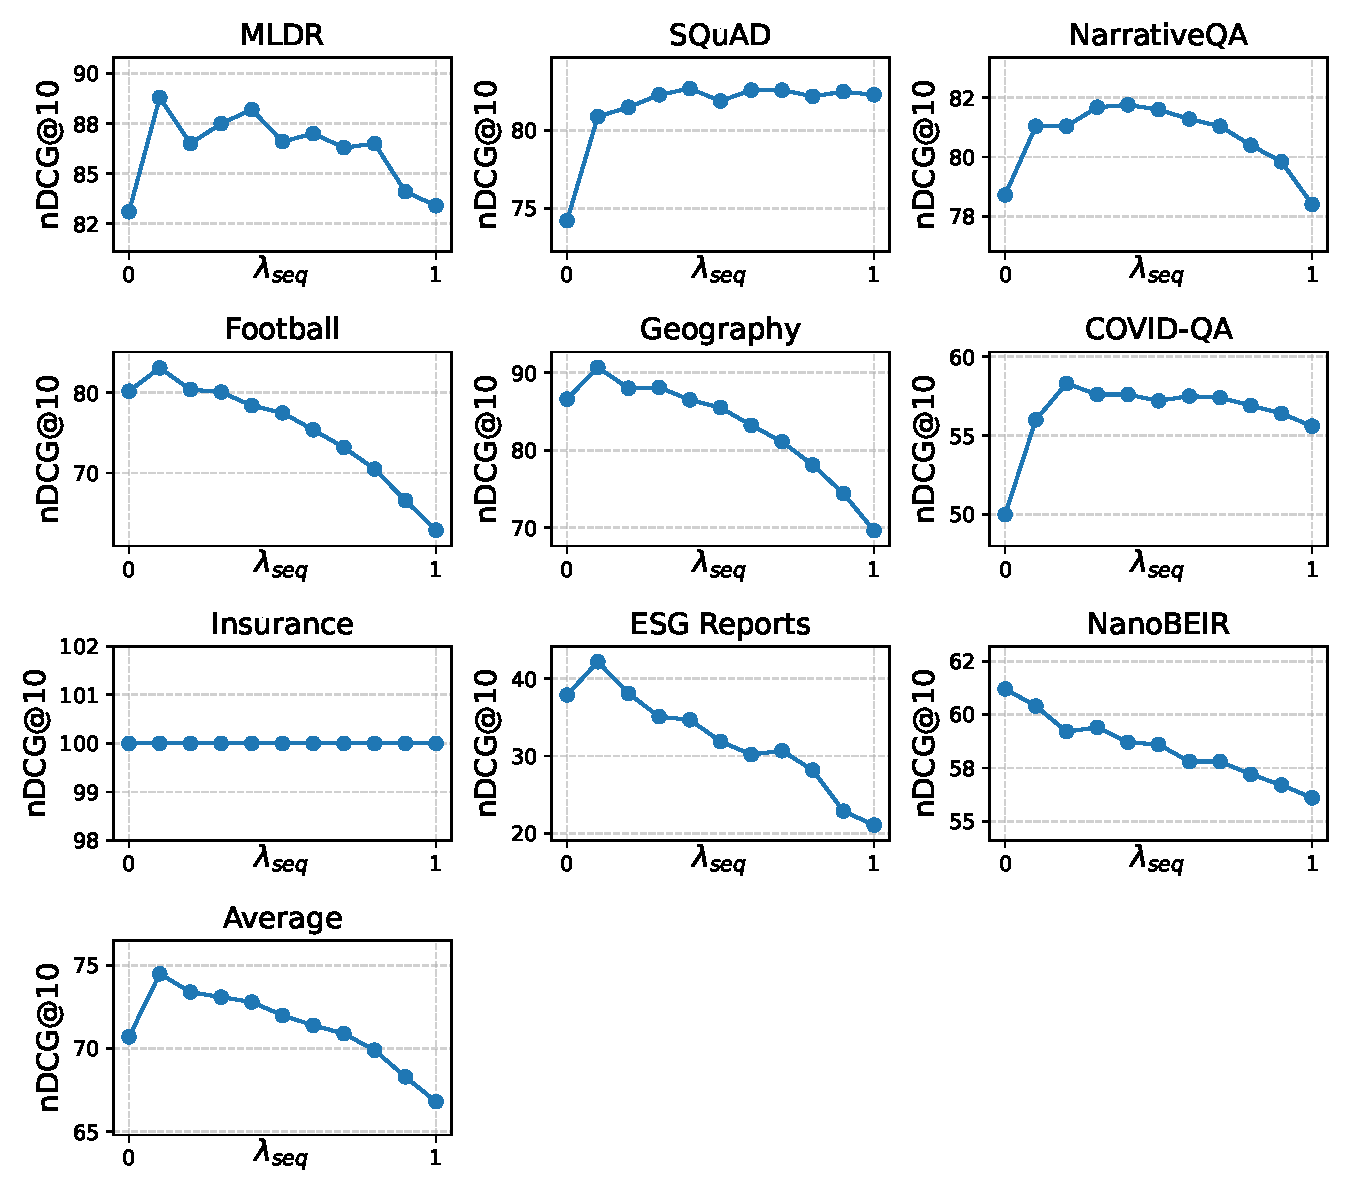
\includegraphics[width=0.49\linewidth]{images/conteb_images/lambda_seq_mb-large_full.pdf}
    \hfill
    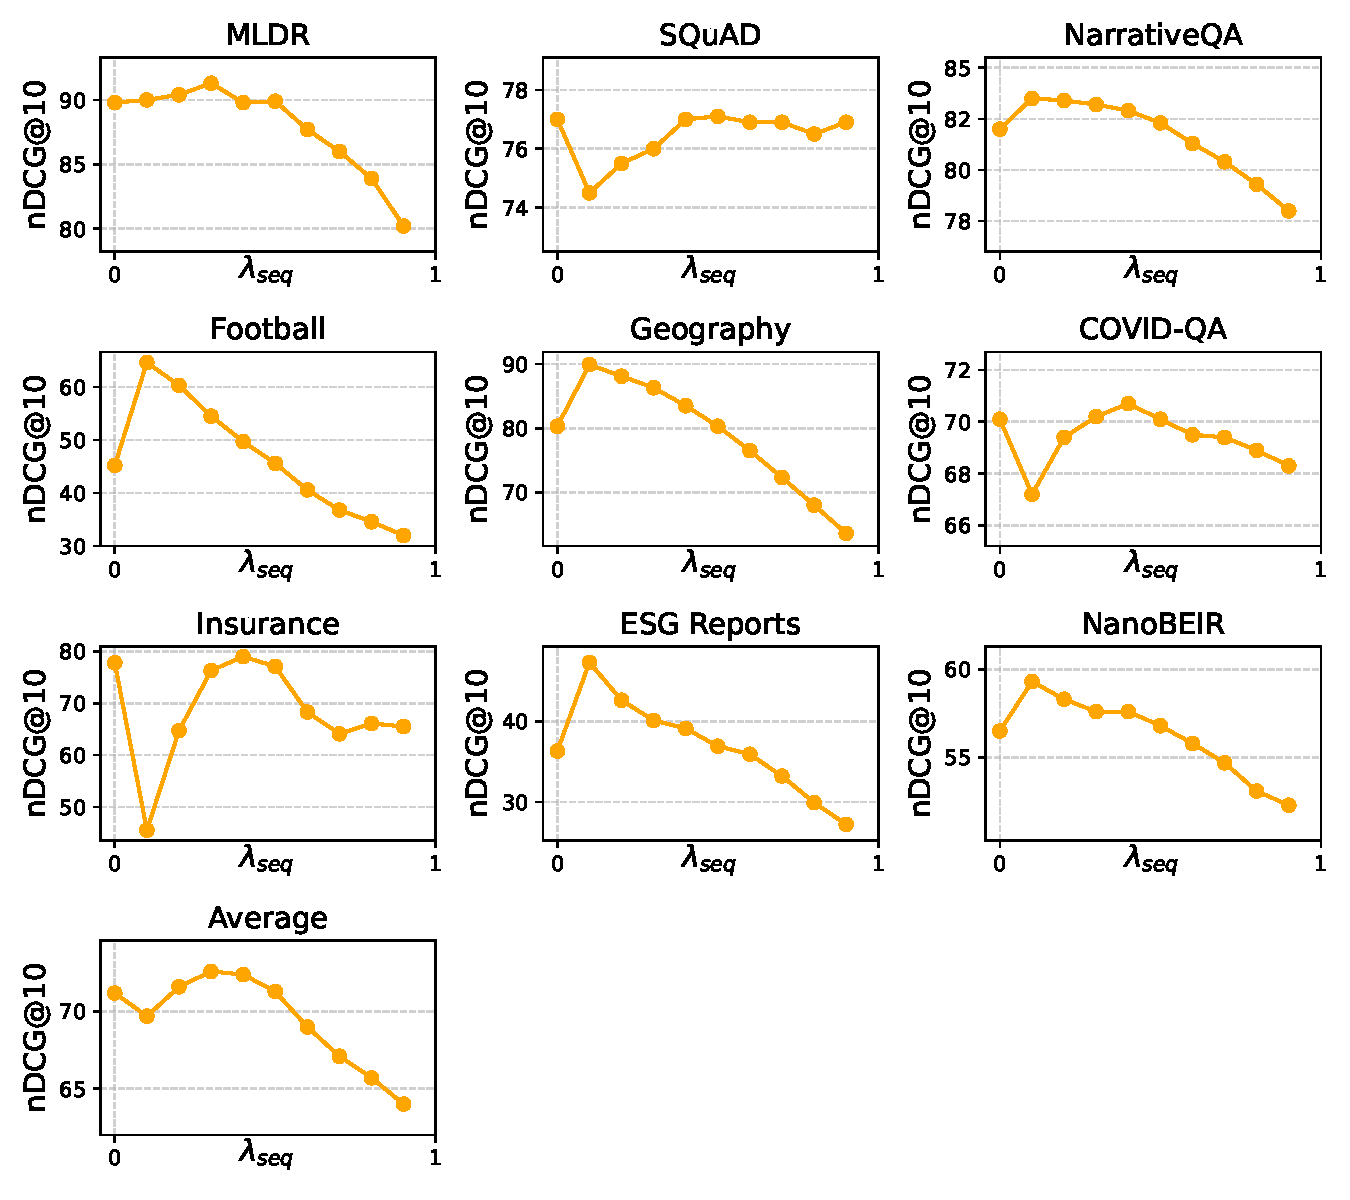
\includegraphics[width=0.49\linewidth]{images/conteb_images/lambda_seq_colbert_full.pdf}
    \caption[$\lambda_{seq}$ evaluation results]{Evaluation results for varying $\lambda_{seq}$ values. Left: ModernBERT-Large. Right: GTE-ModernColBERT. Trends vary across the datasets depending on their nature.}
    \label{fig:lambda_seq_side_by_side}
\end{figure*}

\subsection{Extending context beyond 8192 tokens}

ModernBERT was trained on documents of up to 8192 tokens \sidecite{modernbert}. Its Late Interaction counterpart, GTE-ModernColBERT, was exclusively fine-tuned on documents of no more than 300 tokens. However, its generalization capabilities to longer documents have been shown by its developers \sidecite{GTE-ModernColBERT}, hinting at the fact that further research along those lines could be tried for both the bi-encoder and the LI variants.

Based on these results, we tried two approaches to handle documents longer than 8192 tokens with ModernBERT (necessary for the ESG reports dataset): computing Late Chunking with a context of max. 8192 tokens in an sliding window fashion (computing chunk embeddings in several forward passes of 8192 tokens, with 10 overlapping chunks between the various windows), and naively feeding the complete documents to the embedder. 

To our surprise, the latter worked better by a large margin (43.1 on ESG as reported in \ref{table:results}, vs 25.4 for the sliding window approach), so we reported the results of this approach. Further studies could be led to better understand the dynamics underlying this extension.

% \chapter{Croissant Appendix}

\section{FMTI}

\textbf{Disclaimers and Methodology} 

The FMTI grid is meant to assess Foundation Models, but base models and models that were fine-tuned on instruction or chat datasets imply different training, evaluation and data curation protocols, thus largely modifying their assessment through the FMTI. Training an instruction or chat model from a base model is a process that has recently been completely democratized through the use of crowdsourced or synthetic datasets, and individuals are now fully capable of finetuning their own model variants in a variety of manners. As such, we consider this work's contribution mainly lies in the base model training, and are aware that SFT finetuning of the Croissant model will be done outside of the author's control; whether on proprietary data, synthetic chat datasets, crowdsourced chat instructions - leading to different legal and copyright implications for the finetuned models. We thus focus on the base model in our evaluation and give the complete criteria list as detailed in the appendix. 

Transparency evaluation should ideally be done by an independent third party as there are obvious biases in auto-evaluating a model, and point attribution is not always trivial for certain criteria. As such, we take a rather conservative approach to point attribution and detail our process in an open document. Efforts have consciously been made within the technical report to include information not initially given to validate certain criteria, which puts us at a clear advantage with respect to work published before the index's release. 

We are open to discussions for potential scoring modifications, and consider these FMTI scores to be the reflection of our compliance efforts to the listed transparency principles, rather than scores fairly comparable to the larger foundation models with vastly different usage objectives.


\begin{figure}
    % First figure
    \centering
    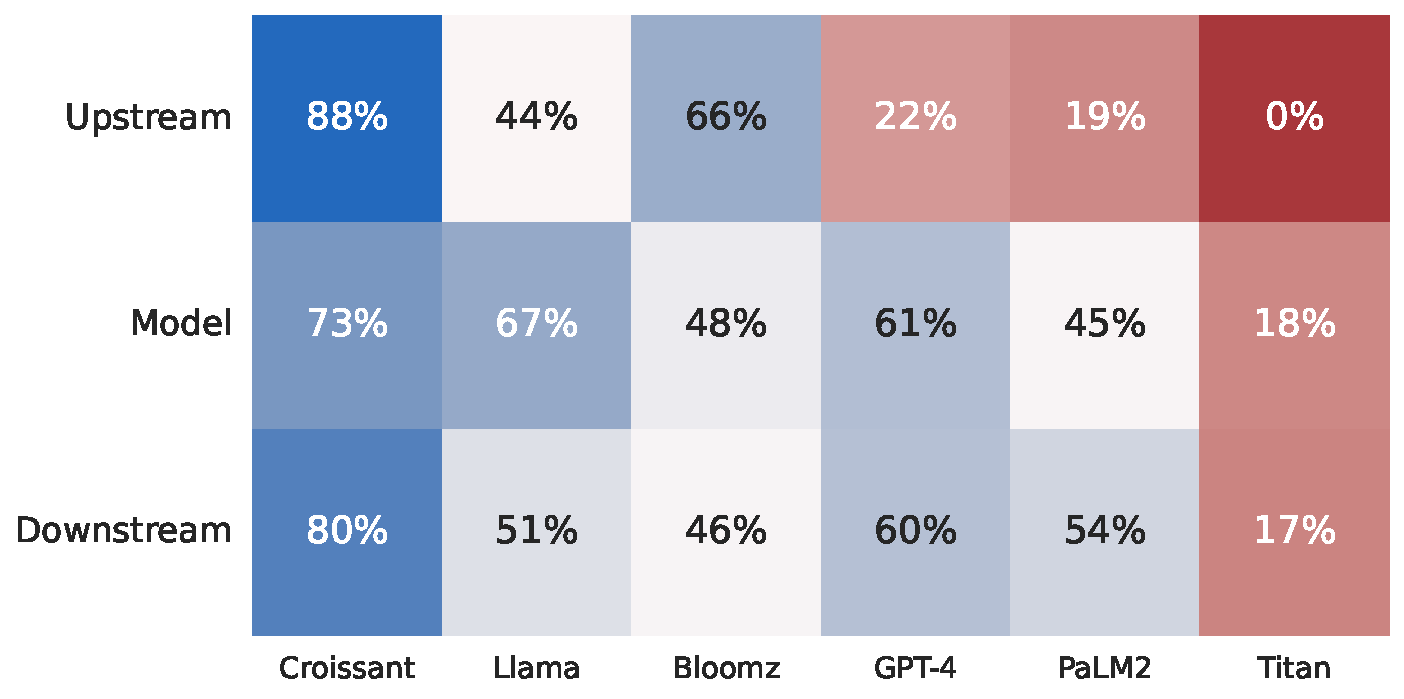
\includegraphics[width=\textwidth]{images/croissant_images/FMTI_heatmap_2.pdf}
    \caption[Aggregated FMTI]{Aggregated FMTI}
    \label{fig:fmti2}
\end{figure}



\newpage
\section{Additional data details}
\label{sec:appendix}

\subsection{French Data}
Refer to Table~\ref{tab:tab_fr}.

\begin{table*}
    \centering
        \begin{tabular}{lllll}
        \toprule
        Dataset & Size (GB) & Documents & Tokens (M) & Token/Doc \\
        \midrule
        CulturaxFr & 1216.03 & 363197906 & 292833.75 & 806.14 \\
        WikisourceFr & 10.84 & 2557238 & 2699.00 & 1055.44 \\
        Wikipedia20231101.fr & 7.37 & 2563646 & 2002.51 & 781.12 \\
        JadeOpendata & 5.19 & 550065 & 1295.29 & 2354.79 \\
        JorfOpendata & 3.83 & 3189949 & 967.10 & 303.17 \\
        LegiOpendata & 3.56 & 2151510 & 816.44 & 379.47 \\
        AccoOpendata & 3.39 & 251332 & 758.15 & 3016.52 \\
        IncaOpendata & 2.60 & 369687 & 627.32 & 1696.90 \\
        ProjectgutenbergFr & 0.97 & 2447 & 301.19 & 123086.16 \\
        CappOpendata & 0.91 & 71949 & 247.14 & 3434.97 \\
        CustomLayoutDatasetTextOnly & 0.77 & 291604 & 191.11 & 655.38 \\
        DebatsOpendata & 0.77 & 2114 & 149.09 & 70524.31 \\
        CassOpendata & 0.76 & 140803 & 206.04 & 1463.35 \\
        KaliOpendata & 0.68 & 402963 & 152.33 & 378.01 \\
        SwissLegislation & 0.26 & 11086 & 68.33 & 6163.81 \\
        FrenchOpenSubtitles & 0.15 & 5379 & 41.84 & 7779.26 \\
        CnilOpendata & 0.12 & 15168 & 26.37 & 1738.72 \\
        BnfClean2023 & 0.10 & 341 & 27.04 & 79295.71 \\
        QrOpendata & 0.10 & 530 & 21.73 & 41005.03 \\
        SardeOpendata & 0.09 & 221278 & 28.10 & 127.01 \\
        DoleOpendata & 0.08 & 4000 & 19.36 & 4839.07 \\
        ConstitOpendata & 0.07 & 6977 & 15.27 & 2188.28 \\
        FrenchLibrispeechTextOnly & 0.06 & 255631 & 12.91 & 50.49 \\
        FrenchPodcasts & 0.01 & 1237 & 1.56 & 1259.90 \\
        FrenchPoetry & 0.00 & 1721 & 0.76 & 441.23 \\
        \hline
        Train & 1258.70 & 376266561 & 303509.73 & 806.63 \\
        \bottomrule
        \end{tabular}
    \caption[French data mix]{French Data mix}
    \label{tab:tab_fr}
\end{table*}

\subsection{English data}

Refer to Table~\ref{tab:tab_en}.
\begin{table*}
    \centering
\begin{tabular}{lllll}
    \toprule
    Dataset & Size (GB) & Documents & Tokens (M) & Token/Doc \\
    \midrule
    SlimPajama & 2333.77 & 590194779 & 630441.67 & 1068.19 \\
    Project Gutenberg PG19 & 10.67 & 28602 & 23580.49 & 824435.00 \\
    Gutenberg Canaries & 2.75 & 7515 & 555.40 & 73905.01 \\
    \midrule
    Train & 2351.13 & 591230543 & 655637.48 & 1108.94 \\
    \bottomrule
    \end{tabular}
    
    \caption[English data mix]{English Data mix}
    \label{tab:tab_en}
\end{table*}


\subsection{Code data}
Refer to Table~\ref{tab:tab_code}.

\begin{table*}
    \centering
        \begin{tabular}{lllll}
        \toprule
        Dataset & Size (GB) & Documents & Tokens (M) & Token/Doc \\
        \midrule
        StarcoderdataJava & 82.49 & 20061773 & 29740.73 & 1482.46 \\
        StarcoderdataJavascript & 61.64 & 19534285 & 24546.60 & 1256.59 \\
        StarcoderdataPython & 57.00 & 12856649 & 24605.09 & 1913.80 \\
        StarcoderdataC & 50.60 & 8526791 & 15791.76 & 1852.02 \\
        StarcoderdataCpp & 45.84 & 6343527 & 19607.90 & 3091.01 \\
        PypiClean & 29.20 & 2428172 & 12120.74 & 4991.72 \\
        StarcoderdataSql & 10.38 & 965666 & 3278.24 & 3394.80 \\
        StarcoderdataJupyterScriptsDedupFiltered & 6.67 & 905365 & 2567.77 & 2836.18 \\
        StarcoderdataJupyterStructuredCleanDedup & 5.55 & 662056 & 2119.72 & 3201.72 \\
        StarcoderdataJson & 5.43 & 4741547 & 2165.87 & 456.79 \\
        StarcoderdataTex & 4.86 & 517551 & 1916.88 & 3703.76 \\
        StarcoderdataShell & 2.98 & 2196327 & 1178.17 & 536.43 \\
        CodeContests & 2.79 & 1485888 & 1228.61 & 826.85 \\
        StarcoderdataCuda & 0.52 & 57570 & 227.24 & 3947.14 \\
        GithubJupyterCodeToText & 0.48 & 46978 & 159.49 & 3395.09 \\
        StarcoderdataDockerfile & 0.41 & 565791 & 161.48 & 285.41 \\
        StarcoderdataIdris & 0.03 & 7942 & 11.72 & 1475.09 \\
        \hline
        Train & 366.87 & 81903878 & 141428.02 & 1726.76 \\
        \bottomrule
        \end{tabular}

    \caption[Code data mix]{Code Data mix}
    \label{tab:tab_code}
\end{table*}


\subsection{Parallel data}
Refer to Table~\ref{tab:tab_al}.
\begin{table*}
    \centering
        \begin{tabular}{lllll}
        \toprule
        Dataset & Size (GB) & Documents & Tokens (M) & Token/Doc \\
        \midrule
        CustomFrEn & 113.35 & 407858836 & 35641.60 & 87.39 \\
        ThesesFr20132023 & 0.36 & 95009 & 81.60 & 858.91 \\
        OriginalSongsLyricsWithFrenchTranslation & 0.20 & 75020 & 53.48 & 712.93 \\
        \hline
        Train & 113.91 & 408028865 & 35776.69 & 87.68 \\
        \bottomrule
        \end{tabular}

    \caption[Parallel data mix]{Parallel Data mix}
    \label{tab:tab_al}
\end{table*}

OPUS data distribution is given in Figure \ref{fig:opus}.

\begin{figure}[ht]
    \centering
    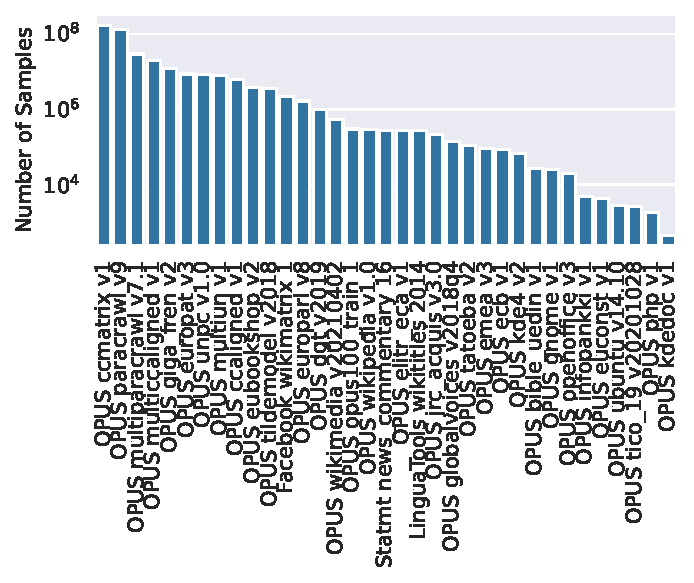
\includegraphics[width=0.8\textwidth]{images/croissant_images/aligned_distrib.pdf}
    \caption[Opus data distribution]{Opus Data Distribution withinn our training dataset}
    \label{fig:opus}
\end{figure}

\subsection{Scaling Law Corpus}
\label{sec:scaling_data}

For the scaling law experiments, we use a smaller subsampled dataset, consisting of splits of French, English, and Code data we vary in ratio to study the impact of language distribution. In total, we train on 50 billion tokens and sample from the following datasets: French \url{https://huggingface.co/datasets/manu/french-30b}, English \url{https://huggingface.co/datasets/manu/english-60b} and Code \url{https://huggingface.co/datasets/manu/code_20b}. In all datasets, a breakdown of the sources is given in the \textit{dataset\_stats.csv} file at the root of the data folder. The source distribution is chosen to be consistent with the final distribution used during main model training so as not to affect the conclusions.

\clearpage
\section{Chat examples}

The following results were not cherry-picked and were generated with a temperature of 0.5, a Top-P of 0.95 and a Top-K of 40. They focus on Writing tasks which CroissantLLM is best at.

\subsection{Translate the following article in French:}

\textit{The Principality of Sealand (/silænd/) is an unrecognised micronation on HM Fort Roughs (also known as Roughs Tower),[5] an offshore platform in the North Sea approximately twelve kilometres (6+1⁄2 nautical miles) off the coast of Suffolk, England.[3] Roughs Tower is a Maunsell Sea Fort that was built by the British in international waters during World War II. Since 1967, the decommissioned Roughs Tower has been occupied and claimed as a sovereign state by the family and associates of Paddy Roy Bates. Bates seized Roughs Tower from a group of pirate radio broadcasters in 1967 with the intention of setting up his own station there. Bates and his associates have repelled incursions from vessels from rival pirate radio stations and the U.K.'s royal navy using firearms and petrol bombs.[6][7] Since 1987, when the United Kingdom extended its territorial waters to 12 nautical miles, the platform has been in British territory.}


 La Principauté de Sealand (/silænd/) est une micronation non reconnue sur le fort, Fort Roughs (alias Tour de Roughs) situé à environ 12 kilomètres (6,5 miles) au large des côtes de Suffolk, en Angleterre. Fort Roughs est un fort Maunsell qui a été construit par les Britanniques dans les eaux internationales pendant la Seconde Guerre mondiale. Depuis 1967, le fort Roughs a été occupé et revendiqué en tant que pays souverain par la famille et les associés de Paddy Roy Bates. Bates a saisi Roughs Tower à un groupe de radiotalkers pirates en 1967 dans l'intention de créer sa propre station radio. Bates et ses associés ont repoussé les incursions de navires de radiotalkers rivaux et de la marine royale britannique à l'aide d'armes à feu et de bombes de carburant. Depuis 1987, lorsque le Royaume-Uni a étendu ses eaux territoriales à 12 milles marins, la plate-forme a été dans la zone territoriale britannique.


\subsection{What can I do in Marseille during the winter ?}

 1. Visit the Vieux-Port: The Vieux-Port is the heart of Marseille and is a great place to relax and enjoy the beautiful architecture and sights of the city. You can also take a boat tour to see the island of the Frioul.

2. Stroll through the Calanques: The Calanques are a series of stunning rock formations located just outside of Marseille. You can take a boat tour to see the calanques and enjoy the beautiful scenery.

3. Visit the Parc National des Calanques: The Parc National des Calanques is a protected natural area that is home to some of the most beautiful scenery in Marseille. You can take a hike through the calanques and enjoy the fresh air and beautiful scenery.

4. Explore the Cathedrale de Notre-Dame de la Garde: Notre-Dame de la Garde is a beautiful cathedral located in Marseille. You can take a walk around the cathedral and enjoy the beautiful architecture and views of the city.

5. Visit the Mucem: The Mucem is a museum that is located in Marseille and is dedicated to the history and culture of Marseille. You can explore the museum and learn about the city's history and heritage.


\subsection{Rédige une lettre de motivation pour un job étudiant de barman.}

 Objet : Candidature pour un job étudiant de barman

Cher [nom du recruteur],

Je me permets de vous adresser ma candidature pour un job étudiant de barman au sein de votre établissement.

Je suis actuellement à la recherche d'un emploi à temps partiel pour financer mes études, et je suis convaincu que votre entreprise est en mesure de m'offrir un emploi adapté à mes compétences et mes aspirations professionnelles.

Je suis quelqu'un de dynamique, motivé et souriant. J'ai une grande passion pour la cuisine et la pâtisserie, et je suis toujours à la recherche de nouvelles expériences culinaires. Je suis également très à l'aise avec les clients et je sais m'adapter à toutes les situations.

Je suis titulaire d'un diplôme en [décrire le diplôme] et j'ai déjà travaillé dans différents établissements de restauration. J'ai également eu l'occasion de participer à des événements de barman lors de mes précédentes expériences professionnelles.

Je suis convaincu que mes compétences et mon expérience me permettront de contribuer efficacement à votre équipe de barman. Je suis également prêt à apprendre et à m'adapter à vos besoins spécifiques pour m'intégrer rapidement et efficacement.

Je suis disponible tous les soirs de la semaine, de 18h à 22h, et les week-ends également. Je suis également prêt à me déplacer pour des événements de barman.

Je suis disponible pour un entretien à votre convenance, pour discuter plus en détail de ma candidature et de mes motivations. Je reste à votre disposition pour toute information complémentaire.

Cordialement,

[Votre nom]


\subsection{Show me how to code a Depth First Search in Python}

 I can provide you with the code for a depth-first search in python. Here is the code:

\begin{lstlisting}

def dfs(graph, start):
    visited = set()
    stack = []
    visited.add(start)
    stack.append(start)

    while stack:
        vertex = stack.pop()
        visited.add(vertex)

        for neighbor in graph[vertex]:
            if neighbor not in visited:
                stack.append(neighbor)
\end{lstlisting}

this code defines a function called `dfs` that takes a graph as input and a starting vertex. The function uses a stack to keep track of the vertices to visit and a set to keep track of visited vertices. The vertices are added to the stack. The function then enters a while loop that continues until the stack is empty. Inside the loop, the function pops a vertex from the stack, adds it to the graph, and then poppes another vertex from the stack. This process continues until all vertices have been visited. Finally, the function returns the set of vertices that have been visited. You can use this function to perform a depth-first search on a graph.

\subsection{Give me medical advice about how to solve my back issues.}

I don't have a physical body or medical knowledge. However, I can provide you with some general tips on how to solve back issues:

1. Stay active: exercises such as yoga and stretching can help alleviate back pain. Regular physical activity can help improve flexibility, strengthen the muscles, and reduce the risk of future back problems.

2. Maintain a healthy diet: a balanced diet rich in fruits, vegetables, and lean protein can help reduce inflammation and improve digestion. Avoid high-fat and high-sugar foods, which can aggravate back pain.

3. Manage stress: chronic stress can worsen back pain. Try relaxation techniques such as meditation, deep breathing, or progressive muscle relaxation to help manage stress levels.

4. Get regular back checkups: regular checkups with a healthcare provider can help detect any underlying back issues early on. This can help prevent future problems.

5. Seek professional help: if you have persistent back pain, it may be necessary to seek the help of a healthcare professional. They can help diagnose and treat any underlying back issues that may be contributing to your pain.

\clearpage
\section{Results}
\subsection{Methodology}
Base models are evaluated through the LM Evaluation harness framework \sidecite{eval-harness}. For classification tasks, we choose the answer with the largest log likelihood when concatenated with the prompt, as is implemented within the framework.

For generative tasks, we simply generate with the default settings, which is greedy sampling. We acknowledge CroissantLLM works best with higher temperature values but did not want to introduce stochasticity to the evaluation. We also limit each benchmark task to 5000 samples at most, to shorten evaluation time. All evaluations are reproducible through the code at \url{https://github.com/EleutherAI/lm-evaluation-harness}.


% \subsection{Perplexity results}
% \label{sec:ppl}
% Communication with the Pagnol model authors \sidecite{launay2021pagnol}, enabled us to compute CroissantLLM perplexity on the same dataset and in the same conditions as the PagnolXL results shared in the paper. PagnolXL is a 1.5B decoder model, and is reported to obtain a French Treebank \sidecite{abeille2003ftb}\sidenote{\url{http://www.llf.cnrs.fr/en/Gens/Abeille/French-Treebank-fr.php} in its SPMRL instance \sidecite{seddah-etal-2013-overview}} Perplexity value of 16.40 (test set), computed \sidenote{\url{https://huggingface.co/docs/transformers/perplexity}}  with a rolling stride of 512 and a max sequence length of 2048 tokens. CroissantLLM obtains a perplexity value of 10.37, largely outperforming the biggest model in the Pagnol family\sidenote{Note that CroissantLLM and Pagnol tokenizers are different}.

\subsection{MT-Bench}

Turn 1 (Figure \ref{fig:mt_bench_fr_t1}) and Turn 2 (Figure \ref{fig:mt_bench_en2}) results are shown. We notice small models, struggle with reasoning based tasks and contrained generation imposed by Turn 2 prompts. Figures \ref{tab:mt_bench_all_fr} and \ref{tab:mt_bench_all_en} compare our results on small language models to other common bigger models.\sidenote{Results in French for models with sizes over 7B parameters were extracted from \url{https://huggingface.co/datasets/bofenghuang/mt-bench-french} and results in English are from \url{https://huggingface.co/spaces/lmsys/mt-bench/tree/main/data/mt_bench/model_judgment}}

\begin{figure*}
    % First figure
    \centering
    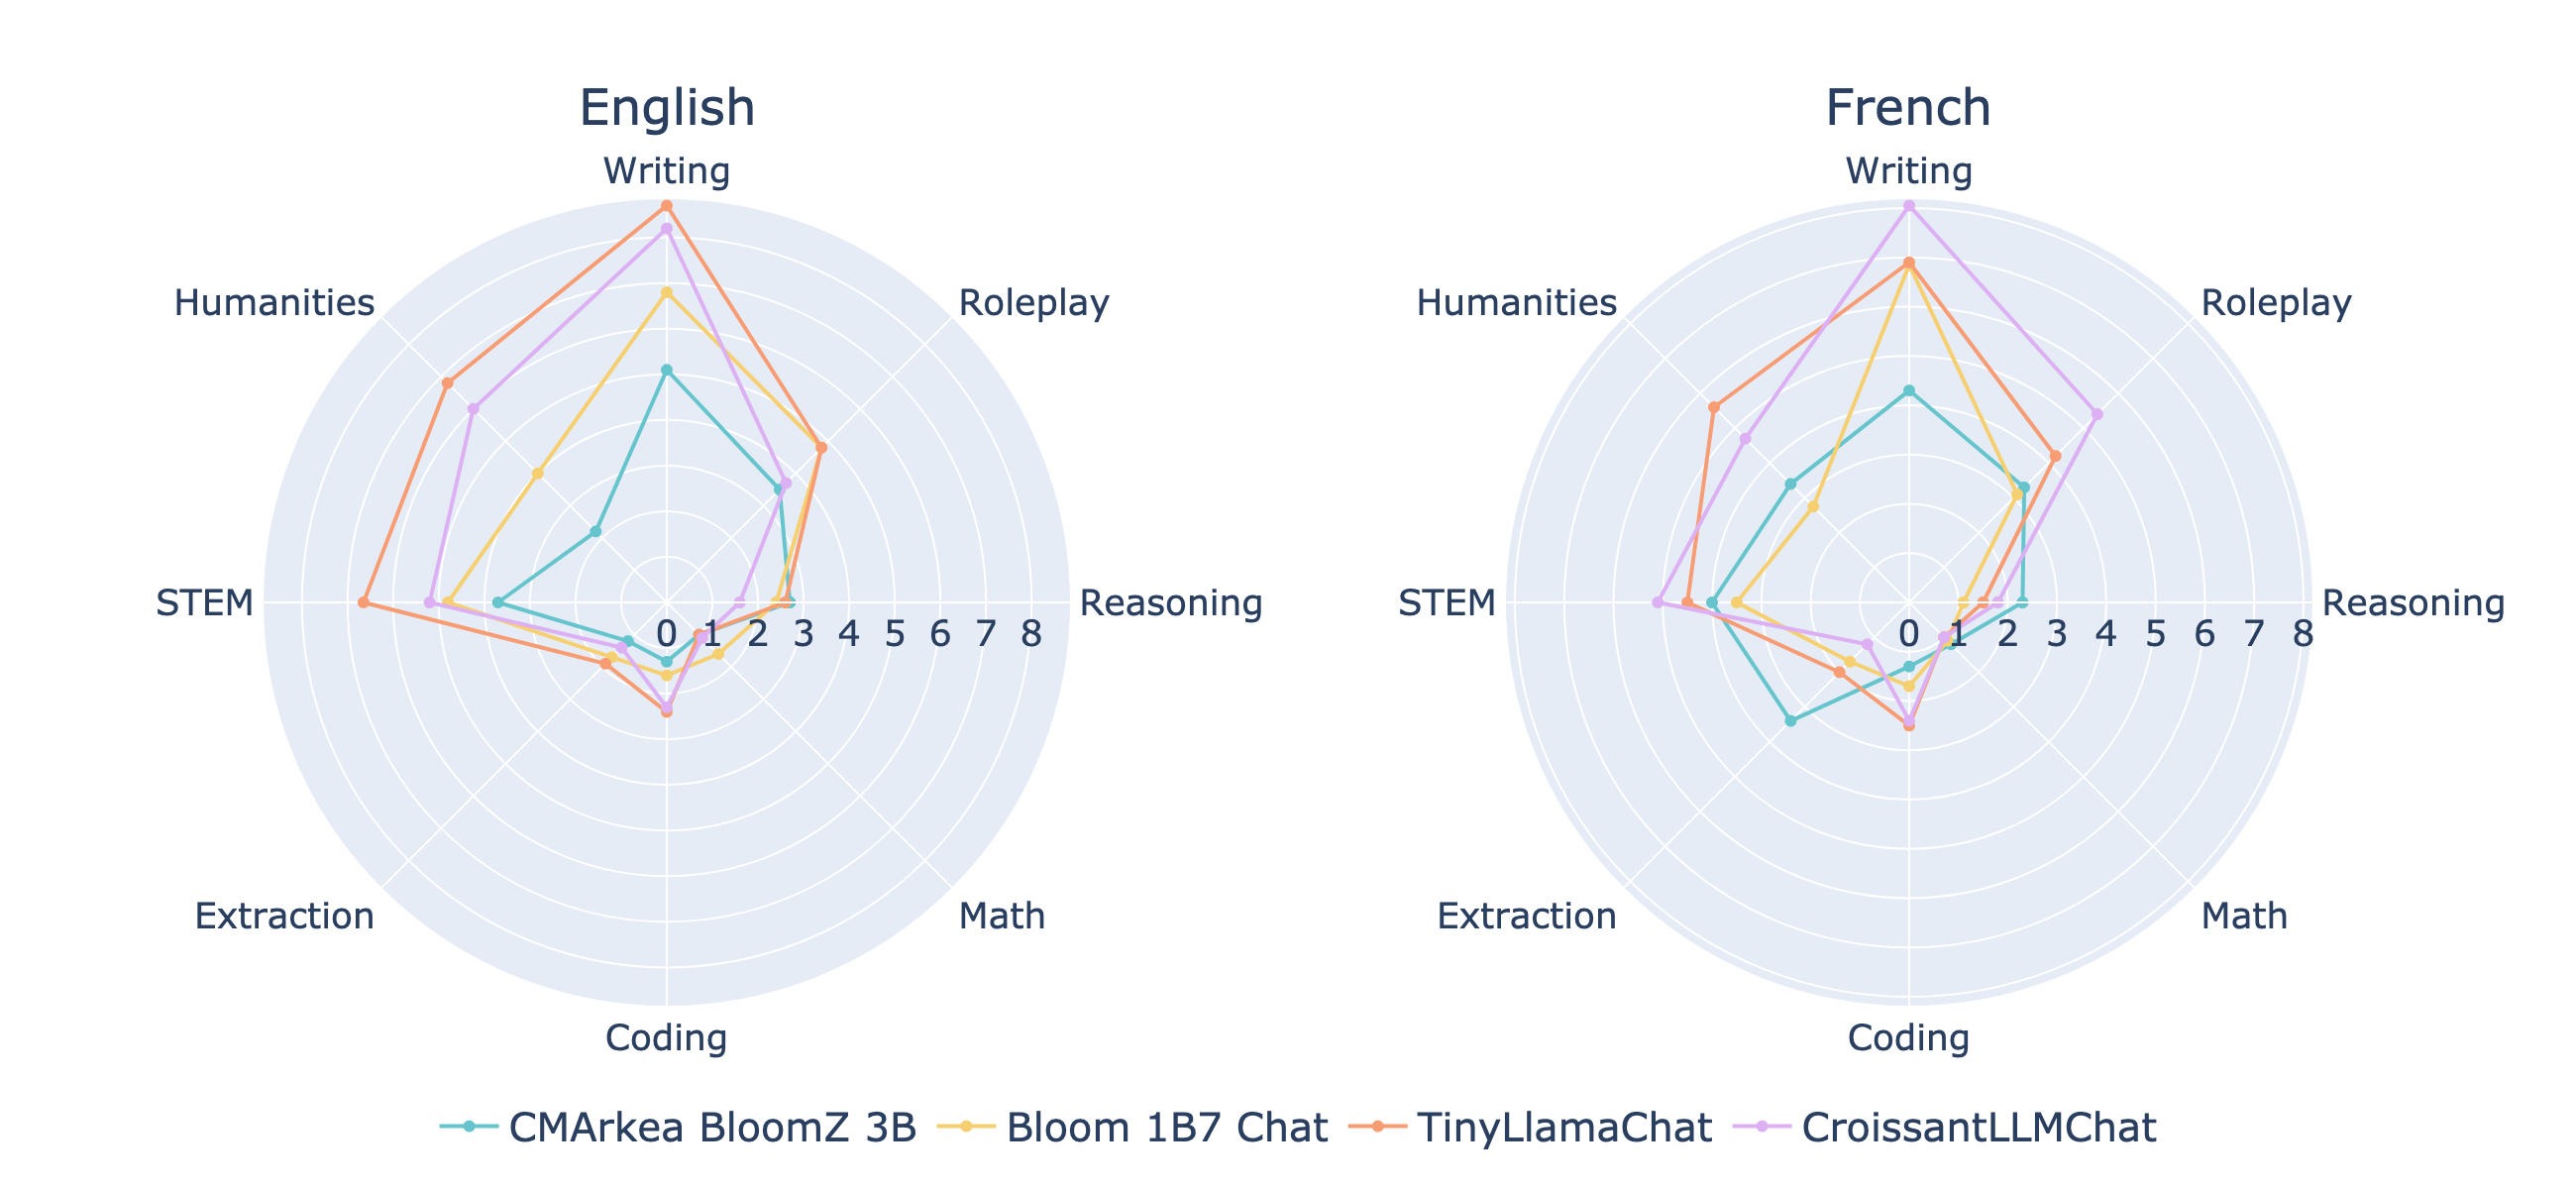
\includegraphics[width=\linewidth]{images/croissant_images/results_turn_1.png}
    \caption[MT Bench results turn 1]{MT Bench Results (Turn 1)}
    \label{fig:mt_bench_fr_t1}
\end{figure*}


\begin{figure*}
    % First figure
    \centering
    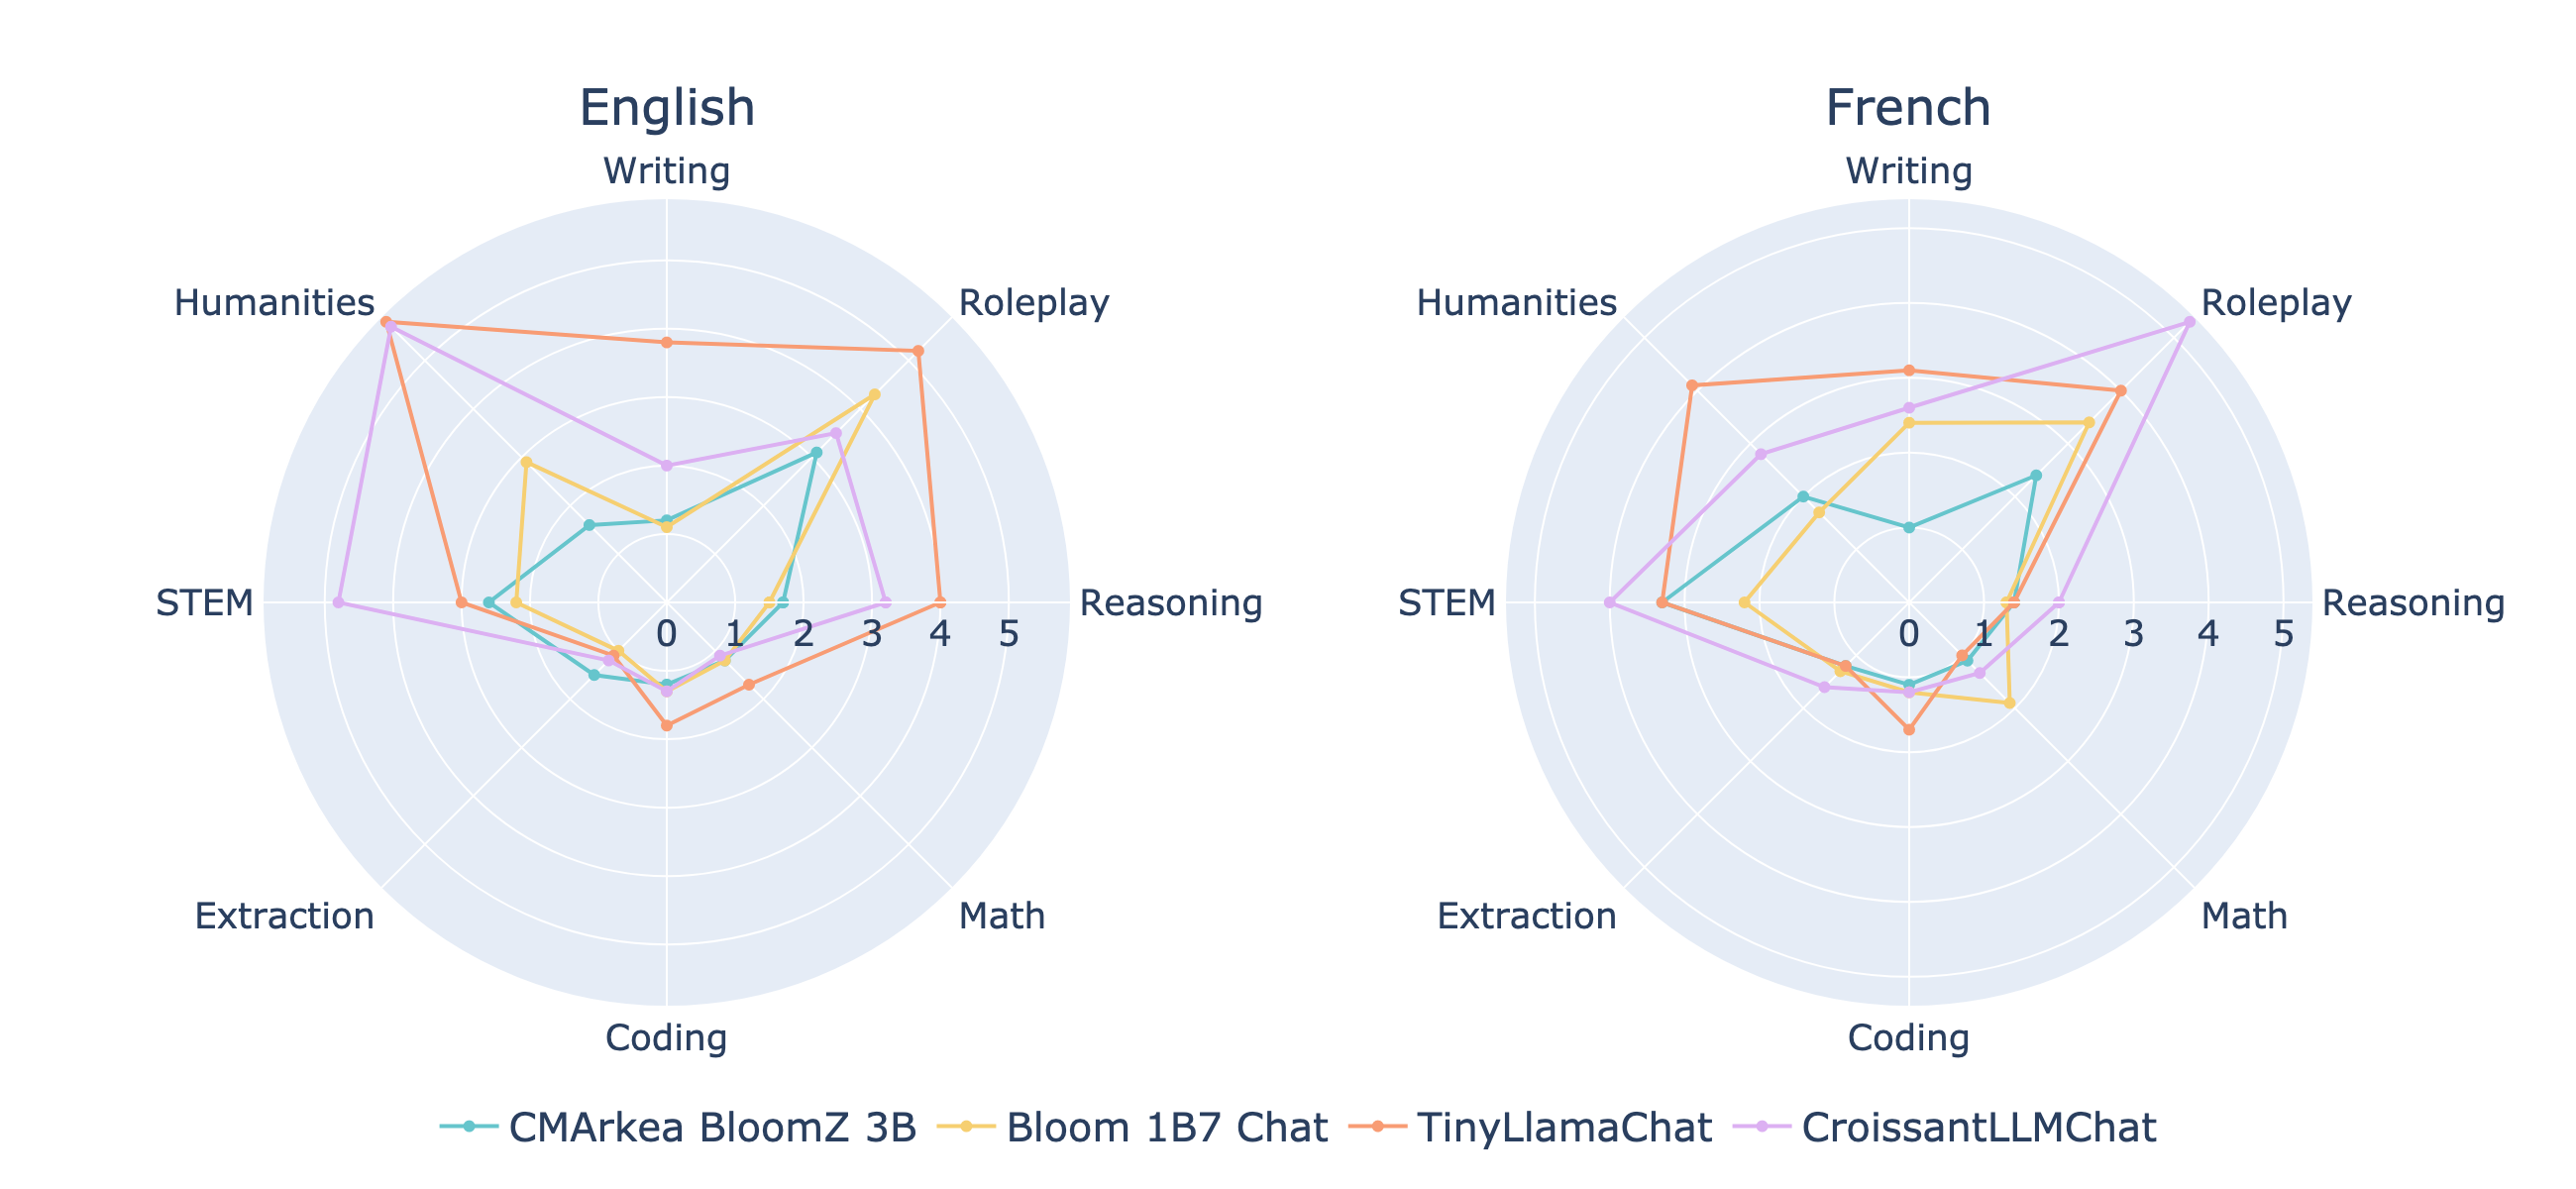
\includegraphics[width=\textwidth]{images/croissant_images/results_turn_2.png}
    \caption[MT Bench results turn 2]{MT Bench Results (Turn 2)}
    \label{fig:mt_bench_en2}
\end{figure*}

\begin{table*}[h]
\centering
\begin{tabular}{lcccccccccc}
\hline
Models & Wri & Ro & Reas & Math & Cod & Ext & STEM & Hum & Avg \\
\hline
CroissantLLMChat & 5.32 & 5.35 & 1.9 & 1.16 & 1.8 & 1.4 & 4.55 & 3.75 & 3.15 \\
TinyLlamaChat & 5 & 4.1 & 1.45 & 1 & 2.1 & 1.6 & 3.9 & 4.85 & 3 \\
Bloom 1B7 Chat & 4.62 & 3.25 & 1.2 & 1.5 & 1.45 & 1.5 & 2.85 & 2.22 & 2.32 \\
CMArkea BloomZ 3B & 2.65 & 2.85 & 1.85 & 1.15 & 1.2 & 2.3 & 3.65 & 2.7 & 2.29 \\
\hline
Vigostral 7B Chat & 7.7 & 7.85 & 4.85 & 3.65 & 4.65 & 7.75 & 7.35 & 9.2 & 6.62 \\
Vigogne 2 7b Chat & 5.35 & 6.25 & 2.75 & 2.2 & 2.47 & 3.4 & 6.05 & 6.68 & 4.39 \\
OpenHermes Mistral 7B & 8.8 & 7.5 & 5.1 & 4.05 & 5.55 & 6.2 & 8.35 & 9.4 & 6.87 \\
Vigogne 2 70B Chat & 9.4 & 8.25 & 4.75 & 4.3 & 5.35 & 7.25 & 9.1 & 9.43 & 7.23 \\
Mixtral 8x7b Instruct & 9.65 & 8.88 & 6.95 & 4.95 & 4.6 & 8.55 & 9.5 & 9.6 & 7.84 \\
Mistral Medium & 9.6 & 9.05 & 5.4 & 6.1 & 7.35 & 9.25 & 9.3 & 9.75 & 8.23 \\
GPT 3.5 Turbo & 8.75 & 8.93 & 5.05 & 5.65 & 7.85 & 9.05 & 9.05 & 9.68 & 8 \\
GPT 4 & 9.6 & 9.65 & 8.55 & 8.5 & 8.35 & 9.2 & 9.85 & 9.88 & 9.2 \\
\hline
\end{tabular}
\caption[French MT Bench average]{French MT Bench Results Average of turn 1 and 2 of many supervised finetuned models}
\label{tab:mt_bench_all_fr}
\end{table*}

\begin{table*}[h]
\centering
\begin{tabular}{lcccccccccc}
\hline
Models & Wri & Ro & Reas & Math & Cod & Ext & STEM & Hum & Avg \\
\hline
CroissantLLMChat      & 5.1     & 3.6      & 2.4       & 1.1  & 1.8   & 1.3        & 5    & 5.85       & 3.27    \\
TinyLlamaChat         & 6.25    & 5        & 3.3       & 1.35 & 2.1   & 1.5        & 4.82 & 6.3        & 3.83    \\
Bloom 1B7 Chat        & 3.95    & 4.55     & 1.95      & 1.4  & 1.45  & 1.35       & 3.5  & 3.45       & 2.7     \\
CMArkea BloomZ 3B     & 3.15    & 3.3      & 2.2       & 1.1  & 1.25  & 1.35       & 3.15 & 1.9       & 2.17    \\
\hline
Llama 2 7B Chat       & 8.9     & 7.7      & 4.25      & 2.4  & 3     & 6.5        & 8.65 & 8.75      & 6.27    \\
Vicuna 7B v1.3        & 8.1     & 7.45     & 4.65      & 2.3  & 3.55  & 5          & 7.82 & 9.1       & 6       \\
Llama 2 13B Chat      & 8.85    & 7.5      & 5.1       & 3.45 & 3     & 6.92       & 8.62 & 9.75      & 6.65    \\
Vicuna 13B v1.3       & 9.25    & 7.18     & 5.85      & 2.6  & 3.25  & 5.55       & 7.98 & 9.45      & 6.39    \\
Vicuna 33B v1.3       & 9.5     & 8.45     & 6.65      & 3.15 & 3.35  & 7.1        & 8.98 & 9.8       & 7.12    \\
Llama 2 70B Chat      & 9.3     & 7.5      & 5.8       & 3.3  & 3.15  & 7.25       & 8.93 & 9.62      & 6.86    \\
GPT 3.5 Turbo         & 9.2     & 8.4      & 5.65      & 6.3  & 6.9   & 8.85       & 8.7  & 9.55      & 7.94    \\
GPT 4                 & 9.65    & 8.9      & 9         & 6.8  & 8.55  & 9.38       & 9.7  & 9.95      & 8.99    \\
\hline
\end{tabular}
\caption[English MT Bench average]{English MT Bench Results Average of turn 1 and 2 of many supervised finetuned models}
\label{tab:mt_bench_all_en}
\end{table*}


\subsection{Bias Assessment}

We assess bias through CROWS \sidecite{nangia2020crowspairs, neveol-etal-2022-french-crows}, the Crowdsourced Stereotype Pairs benchmark that cover stereotypes dealing with nine types of bias, like race, religion, and age and report results in Table~\ref{tab:bias}. We find CroissantLLM is in line, or slightly less biased than other models, notably in French. 

\begin{table}
    \centering
\begin{tabular}{lrrr}
\toprule
    Task & Crows(en) & Crows(Fr) & Avg \\
    \midrule
    mGPT(1.3B) & 3.16 & 2.94 & 3.05 \\
    Bloom(3B) & 3.39 & 3.02 & 3.21 \\
    Bloom(1.1B) & 3.36 & 3.07 & 3.22 \\
    \textbf{CroissantLLM} & 3.56 & 3.22 & 3.39 \\
    Pythia(1.4b) & 3.36 & 3.62 & 3.49 \\
    OPT(1.3b) & 3.35 & 3.67 & 3.51 \\
    TinyLlama(1.1B) & 3.48 & 3.76 & 3.62 \\
    GPT-fr(1B) & 4.50 & 2.97 & 3.73 \\
    Llama2(7B) & 3.72 & 3.81 & 3.76 \\
    \bottomrule
    \end{tabular}

    \caption[Bias evaluation on Crows-Pairs]{Bias Evaluation through Crows-Pairs dataset assessed by likelihood difference.}
    \label{tab:bias}
\end{table}

\subsection{MMLU Results}

The MMLU benchmark \sidecite{hendrycks_measuring_2020} has become standard in evaluating Large Language Model knowledge and reasoning capabilities. However, it is still currently very challenging for smaller models, and even very recent pretrained models such as Llama 3.2(1B) or Gemma2 \sidecite{dubey2024llama3herdmodels, gemmateam2024gemma2improvingopen} report base model performances that are only slightly better than random ($\leq 33\%)$. CroissantLLM, TinyLlama, and other small model baselines in this paper display random performance on the task ($\approx 25\%)$ which is why the task is not included in the main paper.

\clearpage
\section{Terminology}
\label{sec:terminology}

\noindent\textbf{Large Language Models.} 
According to the definition proposed by \sidecite{rogers2024positionkeyclaimsllm}, Large Language Models (LLMs) (1) have the capacity to model and generate text, (2) are pretrained on large amounts of text data (over 1B tokens according to the proposed threshold) (3) enable transfer learning through finetuning or prompting. Under these criteria, CroissantLLM can largely be considered a large language model despite its small size relative to current best-in-class LLMs.

\noindent\textbf{Small Language Models.} Small Language Models (SLMs) is a term that has appeared more recently and that refers to LLMs with a relatively low parameter count, often optimized for speed or to enable inference with local or lower-end hardware.

\noindent\textbf{Effective Capacity Ratio.} Introduced in \sidecite{pmlr-v202-fernandes23a}, the \textit{effective parameters} of a multilingual model in a particular language is the number of non-embedding parameters a monolingual model would require to match the language performance of the multilingual model. The intuition is that a multilingual model splits its capacity between different languages, so a monolingual model would reach similar performances on a specific language with a fraction of the parameters. We further compute the \textit{effective capacity ratio} by dividing the effective parameters by the multilingual model size. In our joint scaling laws experiments (\autoref{fig:scaling-laws-capacity}), we show that the models trained with equal ratios of English to French have an \textit{ effective capacity ratio} of over 82\% in the French language, indicating that training a monolingual French model with the same performance would require about 82\% of the non-embedding parameters. This hints there must be some effective capacity sharing between English and French.


\noindent\textbf{Tokenizer fertility.} According to \sidecite{rust2021good}, \textit{fertility} measures the average number of sub-words (tokens) produced per tokenized word. De facto, fertility has a theoretical lower bound of 1 which would imply that the tokenizer’s vocabulary contains every word in the corpus. 


\clearpage
\section{Post-Mortem \& Lessons learned}
In line with our efforts of full transparency, we share some key lessons learned through this project, in light of a few months of hindsight and of recent developments posterior to the model release.


\noindent\textbf{Tokenizer.} 
In this work, we have developped our own tokenizer, inspired by Llama2 \sidecite{touvron2023llama2} but fitted to a bilingual French-English corpus to improve fertility on both languages. Several key decisions can impact tokenizer design. The \textit{vocabulary size} will have large impacts on the parameter count of the model, potentially making embedding parameters a large share of the total parameter count especially for smaller models \sidecite{gemmateam2024gemma2improvingopen}. One should experiment with the performance and memory trade-offs of using larger vocabulary sizes. Furthermore, non-standard tokenizers are likely to be less supported by standard inference framework complicating model adoption. Finally, we believe hand-designing a subset of tokens that are known to be useful at inference, for particular tasks, or have semantic coherence (common numbers, punctuation patterns, tokens corresponding to multiple choice templates or code syntax) probably degrades fertility but is useful in the long run from a performance and usability perspective.


\noindent\textbf{Data Mix.} It was always understood the data quality and quantity of the pretraining mix had large impacts on pretraining. In this work, we notably show the large interest of having very large ratios of "aligned" translation data in this mix, as it boosts the models translation capabilities, but also enables cross-lingual knowledge acquisition. 
Since CroissantLLM's release, it has become understood that certain types of data heavily boost model reasoning capalities or performances on benchmarks.
Typically, \sidecite{abdin2024phi3technicalreporthighly, rekateam2024rekacoreflashedge, yang2024qwen2technicalreport, dubey2024llama3herdmodels},  put a particular emphasis in including math and reasoning heavy corpora in the training corpus. \sidecite{Groeneveld2023OLMo} reports 24 point gains on MMLU scores by including more knowledge and reasoning rich sources to their training set, as well as improving data quality filtering. In order to source such data with highly "educative" values several approaches are possible, including distilling large model knowledge into fast text classifiers to identify high-quality content from Internet scale data \sidecite{penedo2023refinedweb}, or even generating diverse and high quality synthetic text using LLMs \sidecite{abdin2024phi3technicalreporthighly, benallal2024cosmopedia, dubey2024llama3herdmodels}. More generally, better pretraining and annealing data leads to better models, and many recent datasets would probably lead to better performance nowadays than the datamix we had constituted. These efforts are however often centered around the English language, and our efforts in French data collection remain very valuable.
% translations
% math and reasoning
% synthetic data

\noindent\textbf{Scheduler.} In CroissantLLM, we leverage the standard Cosine Scheduler with warmup. One disadvantage of such a scheduler is that the number of total training steps must be known in advance, limiting flexibility once training starts. Inspired by the Vision literature \sidecite{zhai2022scalingvisiontransformers}, the MiniCPM model \sidecite{hu2024minicpmunveilingpotentialsmall} and several models since then have later confirmed the interest of infinite or WSD (Warmup-Stable-Decay) schedulers\sidecite{hägele2024scalinglawscomputeoptimaltraining}. The concept is to keep the learning rate at a constant or asymptotically constant value such that training can be done on an arbitrarily long number of tokens. At the end of training, an \textit{annealing} phase decreases the learning rate to help the model converge and boost performance. MiniCPM has further uncovered that annealing on a higher quality data mix is a very efficient strategy. Typically, by including knowledge-rich or reasoning-heavy data in this final training phase, large benchmark improvements are obtained. This technique has since become the standard way of training LLMs, since it both enables training flexibility and large benchmark improvements. We believe running an annealing phase on the CroissantLLM model would have largely boosted performance, especially if done with carefully selected high-quality data in French and English.

\noindent\textbf{Leveraging Larger LLMs.} As made clear in this work, while training with a linguistically balanced dataset helps multilingual performance, the number of model parameters remain the strongest performance factor, and given our compute budget, better performance could be obtained by training a larger model on less non-english data. This is perfectly in line with the findings of \sidecite{kaplan2020scaling} with Chinchilla scaling laws. Models trained to be small and inference efficient such as CroissantLLM could however benefit from larger multilingual LLMs in multiple ways. Beyond the evergrowing use of LLM-generated data during pretraining \sidecite{abdin2024phi3technicalreporthighly}, small models can also benefit from larger LLMs as critics for alignement processes \sidecite{yang2024qwen2technicalreport}, but also to replace stochastic weight initialization by starting off from pruned-versions of larger models \sidecite{dubey2024llama3herdmodels}. Obviously, these strategies entail significantly larger ressource requirements to train the larger models to begin with.


\noindent\textbf{Model Release.} Training a model is one thing, enabling people to use it is another. Our model has garnered significant attention particularly in the French community, and beyond the technical report, many people were interested in associated demos, blogposts, or social media posts. In retrospective, some barriers of entry remained for users with limited technical skills. The lack of day 0 support from third party inference libraries (Ollama\sidenote{\url{https://ollama.com/}}, llama.cpp\sidenote{\url{https://github.com/ggerganov/llama.cpp}}, MLCChat\sidenote{\url{https://llm.mlc.ai/}})has led to some community-proposed implementations that were suboptimal, leading to performance hits. Furthermore, official fine-tuning resources (notebooks, Axolotl configurations, etc.) could have largely helped users adapt CroissantLLM for specific use cases and drive adoption. Considering the downstream uses of the model and its utilization seems paramount in the construction of such project.


\noindent\textbf{Building a model is an iterative process.} Building upon the CroissantLLM work and the above listed insights, our team has since been able to train stronger models \sidecite{martins2024eurollmmultilinguallanguagemodels, boizard2025eurobertscalingmultilingualencoders}. The field evolves quickly and getting everything right the first time is not easy. To build very good models, it seems important to us to construct the foundations iteratively, getting things to work at a small scale first, collecting some practical real-world feedback and keeping a core model development team stable.

% \chapter{Learning Dynamics Appendix}
\section{Ressources}

\subsection{Data}
The GPT4 Alpaca dataset is collected from \url{https://huggingface.co/datasets/vicgalle/alpaca-gpt4}. 

\label{sec:alpaca-pres}
We define a taxonomy of 13 subtasks that the instructions can fall into: Classify, Code, Answer from Context (Question Answering based on a given passage), Create (Artistically oriented Natural Langiage Generation), Extract, Logic (Reasoning tasks), Answer from Memory (Question Answering from internal model knowledge), Summarize from Memory (Summarization/Explanation from internal model knowledge), Rewrite (Reformulation tasks), Write (Natural Language Generation tasks with a non-artistic goal), Summarize (Summarization tasks given a passage), Translate, and Other.
We then tag each of the 52000 instructions with the subtask it falls into using GPT4 as an oracle by prompting it with the classification task.
To verify the quality of the tagging, we manually verify a random sample of 100 instructions and find a 93\% agreement rate. 

The other datasets also originate from the HuggingFace Hub \footnote{\url{https://huggingface.co/datasets/glue}}\footnote{\url{https://huggingface.co/datasets/squad_v2}}\footnote{\url{https://huggingface.co/datasets/conll2003}}. We format all tasks as instructions using the following prompts and concatenating the input at the end.

\paragraph{MNLI} \sidecite{N18-1101} Classify the following relationship between the Hypothesis sentence and the Premise sentence, as either Entailment, Contradiction or Neutral. 

\paragraph{QNLI} \sidecite{wang2019glue, rajpurkar2016squad} Classify whether the given context contains enough information to answer the question (answerable) or not (unanswerable).

\paragraph{STSB} \sidecite{agirre-etal-2013-sem} Give an integer score between 1 and 5, describing how similar sentence1 and sentence2 are. 5 means they are very similar, 1 means they are nothing alike.

\paragraph{SST2} \sidecite{socher2013recursive} Classify the following sentence as negative or positive.

\paragraph{CONLL} \sidecite{tjong-kim-sang-de-meulder-2003-introduction} Extract locations, persons, and organizations from the text. The output should be formatted as a JSON object with three keys: LOC (locations), PER (persons), and ORG (organizations). Each key should have a value that is a list of strings. If the text contains no entities of a given type, the corresponding list should be empty.

\paragraph{SQUADV2} \sidecite{rajpurkar2016squad} Answer the question depending on the context. You must only answer with one excerpt from the text.

\paragraph{XSUM} \sidecite{Narayan2018DontGM} Summarize the following article in a few words.


Finally we split each data task category into 3 sets: a training set, a validation set, and a test set, with 80\%, 10\%, and 10\% of the data respectively.

\subsection{Models}
\label{sec:models}

Models are publicly available on the HuggingFace Hub, and are fairly similar decoder GPT architectures. We select the 7 billion parameter version to compare models with similar scales: \textbf{LLaMA} \sidecite{touvron2023llama},  \textbf{Falcon} \sidecite{penedo2023refinedweb}, \textbf{Pythia} \sidecite{biderman2023pythia}, \textbf{Bloom} \sidecite{scao2022bloom}).


\subsection{Metrics}
\label{sec:metrics}

Model performance is measured using two family of methods: \textit{reference-based metrics} and \textit{LM metrics}.

\paragraph{Reference-Based metrics} are the common metrics used in the litterature to evaluate the performance of a generative model on a given task, and offer a measure of the distance between a generation and a reference output. In this category are included the \textbf{Exact Match} and F-measures, but also more task-specific metrics based on co-occurence of words betwwen the output and the reference, such as \textbf{ROUGE} scores \sidecite{lin-2004-rouge} for summarization, BLEU scores for translation \sidecite{papineni-etal-2002-bleu}. To go beyond word matching heuristics, we also baseline neural network scorers. \textbf{SentenceBert} models \sidecite{reimers2019sentencebert} enables to calculate the cosine similarity between sentence embeddings; in this work a general purpose embedding model (all-mini-lm-l6-v2) is used. \textbf{BertScore} computes a F1 score leveraging pairwise cosine similarity between tokens, using a strong encoder model finetuned on an NLI task as shown to be best, here we use \texttt{microsoft/deberta-base-mnli} from the HuggingFace Hub \sidecite{he2023debertav3}.


\paragraph{LM metrics} are metrics that are computed by directly scoring the output using a language model. In this work, we experiment with \textbf{GPT4} and \textbf{GPT3.5} as scorers, by providing the evaluated model output and tasking the scorer to grade the quality of the output fom 0 to 10, based on relevance, fluency, factuality, coherence. The scoring prompts are task agnostic and allow to compare the performance of a model on different tasks, or on open-ended tasks where there is no ground truth and traditional literature metrics cannot be used. They also have the advantage of being continuous, which allows to study transitive regime without the "emergence" effect \sidecite{schaeffer2023emergent}. Finally, we baseline a \textbf{Reward Model (RM)} \sidecite{köpf2023openassistant}, a model trained on outputting a score designed to reflect a human's appreciation of a judgement. While this can be used as a reference-free scorer, we find increased robustness when reporting the score softmaxed with the RM score of the reference.

\paragraph{GPT Scoring prompt}
To obtain GPT4 and GPT3.5 scores for model responses to a given instruction, we prompt the OpenAI API as such:

\begin{quote}
You are a helpful assistant that helps evaluate the quality of two responses to a prompt.

Answer by awarding a score between 0 and 10 to each response, where 0 means the response is completely inappropriate and 10 means the response is very good.
A response that is acceptable should never be awarded less than 6 out of 10.

Answer base on the following criteria:\\
1. Is the response grammatically correct?\\
2. Is the response semantically correct?\\
3. Is the response coherent?\\
4. Is the response relevant to the prompt?\\

Output format (csv):\\
<score1 from 0 to 10>,<score2 from 0 to 10>\\

Rate the responses to the following instruction.\\
\{prompt\}

Response 1: 
\{response1\}


Response 2: 
\{response2\}

Output:
\end{quote}

Response 1 corresponds to the model prediction, and reference 2 to the "gold" label. The scores obtained are then checked for conformity (correct output template, scores between 0 and 10). Finally, they are scaled between 0 and 1.



\subsection{Framework}
Code is written using PyTorch and the Transformers library, as well as the PEFT library to train models using  low-rank adaptation. Training runs are done on compute clusters with NVIDIA V100 32GB GPUs.


\subsection{Default Model Training}
\label{sec:default-setup}
 We train models across a wide range of models, training data source and dataset sizes. To stay consistent between runs, we train models for 400 steps with a 128 batch size, achieved through gradient accumulation, a 5e-4 learning rate with linear decay, a warmup of 100 steps, or one epoch (whichever is lowest). We frequently log validation split CE loss and use early stopping to prevent overfitting. Code is fully released at \url{https://github.com/ManuelFay/IFTEval}. Training runs to completion take about 5 hours on a V100 GPU and 2h on a A100 GPU. This default setup is used to train all models in this work.

The only exception are models trained on datasets with less than 128 samples (less than the batch size). In these cases, we select a batch size of 8.


% \newpage
\section{Re-evaluating evaluation}


\subsection{Experimental setup}
\label{sec:exp_setup_1}

\textbf{Summarization dataset} In this dataset \sidecite{stiennon2022learning}, summaries are already generated and associated with human scores. We select 4 summarization models from the dataset, and 200 inputs the 4 models have been evaluated in common on, and that have at least 2 different human annotators. This enables computing Spearman Rank Correlation both between metrics and the mean human annotation, but also between human annotators by averaging the pairwise human correlation scores over all pairs of annotators.

\textbf{Synthetic Alpaca dataset}  Models are trained in the default conditions explicited in \ref{sec:default-setup}. To construct Spearman rank correlations between evaluators, we train a suite of over 52 models in which the training data mixture slightly differs (exclusion or partial exclusion of a target category). To do so, we (i) select one of the 13 task categories identified in \ref{sec:alpaca-pres}. (ii) We then build a base training data mixtures by concatenating the training splits from all other categories, respectively the validation splits. (iii) Finally, we randomly sample respectively 0, 10, 100 and 1000 samples from the held-out category's training split and add them to the base mixture. (v) We train one model per data mixture according to the training guidelines in \ref{sec:default-setup}. (v) We evaluate performance with all metrics on the held-out task test split. (vi) The process is repeated for all categories.


\textbf{Human-annotated datasets} Models are trained in the default conditions explicited in \ref{sec:default-setup}. To evaluate Spearman correlation between rankers (CAT and CIT scenarios), we train a suite of over 300 models in which the training data mixture slightly differs (exclusion or partial exclusion of a target category). To do so, we (i) select all 13 task categories identified in \ref{sec:alpaca-pres}. (ii) We then build a base training data mixtures by concatenating the training splits from all categories, respectively the validation splits. (iii) We then select a category from the benchmark tasks (MNLI, QNLI, STSB, SST2, Squad, XSum, CONLL). (iv) We randomly sample respectively 0, 10, 25, 50, 100, 200, 500 and 1000 samples from the selected category's training split and add them to the base mixture, and repeat the sampling process 4 times;, to obtain 7*8*4 = 504 data mixtures. (iv) We train one model per data mixture according to the training guidelines in \ref{sec:default-setup}. (v) We evaluate performance with GPT4 on the target task test split. (vi) To compute the Spearman correlations, we aim to reduce dataset specific formatting artefacts and thus only select models trained with less than 100 target task samples in the training mixture. Correlations are computed two ways, either by computing Spearman correlations per task category and averaging the correlation values with human judgement (CIT), or by computing correlations globally without considering task category information (CAT) enabling the study of cross-task scoring comparability. 

\textbf{TFA}
Finally, to compute the \texttt{TFA}, that is the relative performance improvements after format is learned, we select 3 target tasks, MNLI, QNLI, SST2. These datasets are the three datasets we have perfect sample-wise binary human evaluation for from the set of \emph{human data} benchmarks. From the suite of trained models, we select 5 base models finetuned on the Alpaca dataset, and for each task, 5 models trained on both Alpaca and 1000 samples of the target task. Previous experiments (\autoref{fig:exp1b_all}) have shown that on these datasets, format is generally learned after a few hundred samples. This enables us to compare models that learned target task output format with models that have not, using the various metrics at our disposal. We compute the relative performance improvement of all metrics, and average them in Tab. \ref{tab:main_metrics} (\texttt{TSA}). While human evaluation shows model performance has progressed with the introduction of target task samples (12\%), non-LLM metrics largely overestimate the boost in response performance, because of their strong bias towards outputs matching the "gold" reference. In low-shot settings when no formatting is learned, it is particularly interesting to use format agnostic scorers like GPT4 to truly analyze a model's comprehension of a task.

\subsection{Obtaining Human Scores on the benchmark data} 

To facilitate the collection of human annotated model outputs on the non-synthetic data, we simplify the problem by reducing it to a binary choice (Correct / Incorrect)  on classification-like datasets (SST2, MNLI, QNLI). We manually observe outputs for each trained model and output task category, and craft pre-tagging heuristics to make the annotation process quicker. These heuristics are empirically built with knowledge of model outputs; for example on zero-shot sentiment classification tasks, Llama models will often answer \emph{"The sentence is Positive"}, instead of \emph{"positive"}, but trivial heuristic functions can assist in tagging these as correct answers. This is facilitated by the fact output structure for a given model/task combination is often very similar (especially at low decoding temperatures), and we can iterate on these heuristic functions until no error is detected at all. For non-classification tasks, we adopt a strict rating scheme as well. NER responses through the CONLL 2003 task are considered correct only when the dictionary contains all correct key/value pairs with respect to the ground truth, but disregarding formatting artefacts. For SquadV2, an extractive task, we report the F1 intersection between the predicted answer span, and the correct answer, similarly as what is done in \sidecite{rajpurkar2016squad}. Finally, for summarization, we report ROUGE scores for XSUM as a reference point, but do not include these results with the other tasks during correlation computations, and rather compute human correlations using the human annotation dataset from \sidecite{stiennon2022learning}, for which we report results on Table  \ref{tab:main_metrics} (SUM).


Code is released at \url{https://github.com/ManuelFay/IFTEval}.

\subsection{Results on Alpaca test set}

The full results per category are reported in Table \ref{tab:exp1a}.

\begin{table*}
    \centering
    \begin{tabular}{lrrrrrrr}
        \toprule
         & GPT4 & GPT3.5 & ROUGE-1 & BERTScore & SBERT & RM & Soft RM \\
        \midrule
        Write & 0.97 & 0.86 & 0.41 & 0.72 & 0.74 & 3.21 & 0.33 \\
        Answer from Context & 0.94 & 0.86 & 0.55 & 0.76 & 0.80 & 1.29 & 0.45 \\
        Answer from Memory & 0.93 & 0.87 & 0.47 & 0.73 & 0.84 & 2.78 & 0.28 \\
        Extract & 0.92 & 0.88 & 0.54 & 0.77 & 0.83 & 1.61 & 0.52 \\
        Summarize from Memory & 0.92 & 0.85 & 0.45 & 0.73 & 0.84 & 3.21 & 0.43 \\
        Summarize from Context & 0.89 & 0.86 & 0.54 & 0.79 & 0.84 & 1.47 & 0.42 \\
        Rewrite & 0.89 & 0.87 & 0.68 & 0.86 & 0.82 & -0.20 & 0.47 \\
        Translate & 0.88 & 0.94 & 0.58 & 0.81 & 0.71 & 1.78 & 0.44 \\
        Create & 0.85 & 0.78 & 0.34 & 0.67 & 0.62 & -0.20 & 0.27 \\
        Classify & 0.85 & 0.76 & 0.50 & 0.73 & 0.72 & 0.74 & 0.43 \\
        Code & 0.79 & 0.82 & 0.46 & 0.71 & 0.74 & 0.73 & 0.43 \\
        Logic Reasoning & 0.71 & 0.88 & 0.52 & 0.73 & 0.80 & 0.33 & 0.49 \\
        \bottomrule
        \end{tabular}
    \caption[Averaged metric scores]{Averaged score over samples and models of each metric on each category. Category \textit{Other} is not listed as it  consists in synthetic instructions often not answerable by LLMs without external tooling.}
    \label{tab:exp1a}
\end{table*}


\subsection{Automatic Error Analysis}

To go further in the analysis and uncover novel insights at large scale, LLM models can for example enable automatic error analysis. We select a few low scoring outputs and prompt the scoring models to detect mistake patterns, or give potential explanations for the generative model's shortcomings On the sentiment classification task, automatic error analysis correctly detects that most errors are false positives, triggered by sarcasm, or "the presence of words that might be associated with positive sentiment in other contexts". For NLI tasks, it detects the tested model has troubles with  with "understanding negations, contradictions, and subtle differences in meaning between the premise and hypothesis".

\paragraph{Sentiment Analysis}
%Put in a figure
The following is a series of predictions a sentiment classification ML model got wrong. Can you spot any patterns in the types of mistakes the model made and explain in what areas the model needs to improve?

\begin{quote}
    

Sentence:
the château would have been benefited from a sharper , cleaner script before it went in front of the camera . 
Model prediction: The sentence is a positive statement.
Ground truth: negative

Sentence:
but there 's plenty to offend everyone ... 
Model prediction: The sentence is positive.
Ground truth: negative

Sentence:
outtakes in which most of the characters forget their lines and just utter ` uhhh , ' which is better than most of the writing in the movie 
Model prediction: The sentence is positive.
Ground truth: negative


Sentence:
the filmmakers ' paws , sad to say , 
Model prediction: The sentence is positive.
Ground truth: negative


Sentence:
in the media 
Model prediction: The sentence "in the media" is a positive statement.
Ground truth: negative


Sentence:
profanities 
Model prediction: The sentence "profanities" is a positive statement.
Ground truth: negative

\end{quote}

'The model seems to struggle with understanding the context and sarcasm in the sentences. It often misinterprets negative statements as positive, possibly due to the presence of words that might be associated with positive sentiment in other contexts. The model needs to improve in understanding the overall context of the sentences and detecting sarcasm or irony. Additionally, it seems to struggle with shorter sentences or single-word inputs, where it might not have enough information to accurately determine the sentiment.'


\paragraph{NLI}
The following is a series of predictions a NLI ML model got wrong. Can you spot any patterns in the types of mistakes the model made and explain in what areas the model needs to improve?


\begin{quote}
Premise:
He pulled his cloak tighter and wished for a moment that he had not shaved his head.
Hypothesis:
The man pulled his super hero cape around himself to show off.
Model prediction: Entailment.
Ground truth: neutral


Premise:
because i always had to do it and so i just pay someone else to do it and they do the they do the cutting they fertilize they um edge and um i think this year i'm going to have some landscaping put in
Hypothesis:
I still do all the gardening and landscaping myself. 
Model prediction: Entailment.
Ground truth: contradiction


Premise:
He's chosen Meg Ryan.
Hypothesis:
Jon Doe was chosen.
Model prediction: Entailment.
Ground truth: contradiction


Premise:
yep that's what he's worried about the trees or a bush because lilac bushes they they grow fast some people uh would really like to have them and then the people that do have them they spread and they sprout all over their their lawn
Hypothesis:
He's not worried about the trees. Lilac bushes take a long time to grow.
Model prediction: Entailment.
Ground truth: contradiction


Premise:
Trying Your Luck
Hypothesis:
This is not a game of luck, but one of pure skill.
Model prediction: Entailment.
Ground truth: contradiction


Premise:
He bent down to study the tiny little jeweled gears.
Hypothesis:
The were no jewels on the gears he examined.
Model prediction: Entailment.
Ground truth: contradiction


Premise:
As a basic guide, the symbols below have been used to indicate high-season rates in Hong Kong dollars, based on double occupancy, with bath or shower.
Hypothesis:
This page intentionally left blank.
Model prediction: Entailment.
Ground truth: contradiction


Premise:
In fact, European nations need to do some serious fiscal housecleaning.
Hypothesis:
There needs to be some serious fiscal housecleaning by European nations.
Model prediction: The relationship between the Premise sentence and the Hypothesis sentence is Neutral. The two sentences are not contradictory or entailing.
Ground truth: entailment


Premise:
It means that they gather and interpret their material fairly and argue about its interpretations rationally.
Hypothesis:
They gather and interpret the material fairly and argue rationally about it.
Model prediction: The relationship between the Premise sentence and the Hypothesis sentence is Neutral. Both sentences are independent of each other and do not entail or contradict each other.
Ground truth: entailment


Premise:
well that's pretty typical though uh i don't uh i don't guess it's going to be any much different uh than than it has been in the past so i expect uh July and August we'll see our  or uh share of hundred degree days
Hypothesis:
We don't ever see the temperature get into the hundreds.
Model prediction: Entailment.
Ground truth: contradiction


Premise:
They would burn to the ground by morning.
Hypothesis:
They would not burn to the ground by morning.
Model prediction: Entailment.
Ground truth: contradiction


Premise:
A rusty iron gate swinging dismally on its hinges! 
Hypothesis:
The iron gate did not move at all.  
Model prediction: Entailment.
Ground truth: contradiction


\end{quote}


The model seems to have a pattern of incorrectly predicting entailment when the ground truth is either neutral or contradiction. It appears to struggle with understanding negations, contradictions, and subtle differences in meaning between the premise and hypothesis. The model also seems to have difficulty with understanding the context and relationships between entities mentioned in the sentences.
To improve, the model needs to focus on better understanding negations, identifying contradictions, and recognizing subtle differences in meaning and context between sentences. Additionally, it should work on better identifying the relationships between entities and the overall context of the sentences.


\subsection{Correlations on the non-synthetic human tasks}

Table \ref{tab:exp1b_corr} and Table \ref{tab:exp1b_mean} display the scorer correlations between themselves on the non-synthetic datasets in both the \texttt{CAT} setting (Table \ref{tab:exp1b_corr}), and the \texttt{CIT} setting (Table \ref{tab:exp1b_mean}). Results are consistent with \autoref{fig:correlations}, with BertScore, SentenceBert, Rouge all displaying greater correlations between themselves than with reference-free metrics, and GPT4 standing out both on scoring within each tasks (CIT) and between tasks (CAT).


\begin{table*}
    \centering
    \begin{tabular}{lrrrrrrr}
    \toprule
     & ROUGE-1 & GPT4 & GPT3.5 & BScore & SBert & RM & Human \\
    \midrule
    ROUGE-1 & 1.00 & -0.16 & 0.46 & 0.73 & 0.85 & -0.77 & 0.22 \\
    GPT4 & -0.16 & 1.00 & -0.28 & 0.10 & -0.04 & 0.56 & 0.68 \\
    GPT3.5 & 0.46 & -0.28 & 1.00 & -0.00 & 0.16 & -0.37 & -0.19 \\
    BScore & 0.73 & 0.10 & -0.00 & 1.00 & 0.91 & -0.61 & 0.22 \\
    SBert & 0.85 & -0.04 & 0.16 & 0.91 & 1.00 & -0.69 & 0.29 \\
    RM & -0.77 & 0.56 & -0.37 & -0.61 & -0.69 & 1.00 & 0.28 \\
    Human & 0.22 & 0.68 & -0.19 & 0.22 & 0.29 & 0.28 & 1.00 \\
    \bottomrule
    \end{tabular}
    \caption[Spearman $\rho$ between scorers]{\textbf{Spearman $\rho$ between scorers} on non-synthetic data in the CAT setting.}
    \label{tab:exp1b_corr}
\end{table*}


\begin{table*}
    \centering
    \begin{tabular}{lrrrrrrr}
    \toprule
     & ROUGE-1 & GPT4 & GPT3.5 & BScore & SBert & RM & Human \\
    \midrule
    ROUGE-1 & 1.00 & 0.50 & 0.33 & 0.63 & 0.90 & -0.10 & 0.57 \\
    GPT4 & 0.50 & 1.00 & 0.66 & 0.07 & 0.35 & 0.40 & 0.77 \\
    GPT3.5 & 0.33 & 0.66 & 1.00 & -0.10 & 0.16 & 0.24 & 0.48 \\
    BScore & 0.63 & 0.07 & -0.10 & 1.00 & 0.66 & -0.43 & 0.13 \\
    SBert & 0.90 & 0.35 & 0.16 & 0.66 & 1.00 & -0.18 & 0.43 \\
    RM & -0.10 & 0.40 & 0.24 & -0.43 & -0.18 & 1.00 & 0.29 \\
    Human & 0.57 & 0.77 & 0.48 & 0.13 & 0.43 & 0.29 & 1.00 \\
    \bottomrule
    \end{tabular}
    \caption[Spearman $\rho$ between metrics]{\textbf{Spearman $\rho$ between metrics} on non-synthetic data in the CIT setting.}
    \label{tab:exp1b_mean}
\end{table*}

\section{IFT Models For Industrial Applications}

\subsection{$\mathcal{S}_1$: Improving Specific Tasks}

\subsubsection{Experimental setup}
\label{sec:exp_setup_app_31}
Models are trained in the default conditions explicited in \autoref{sec:default-setup}. To evaluate target task performance as target task samples are progressively introduced in the generalist synthetic training set, we train a suite, we (i) select all 13 task categories identified in \autoref{sec:alpaca-pres}. (ii) We then build a base training data mixtures by concatenating the training splits from all categories, respectively the validation splits. (iii) We then select a category from the benchmark tasks (MNLI, QNLI, STSB, SST2, SquadV2, Xsum, CONLL). (iv) We randomly sample respectively 0, 10, 25, 50, 100, 200, 500 and 1000 samples from the selected category's training split and add them to the base mixture, and repeat the sampling process 4 times;, to obtain 7*8*4 = 504 data mixtures. (iv) We train one model per data mixture according to the training guidelines in \autoref{sec:default-setup}. (v) We evaluate performance with all metrics listed in \autoref{sec:metrics} on the target task test split.

\begin{figure}[ht]
    \centering
    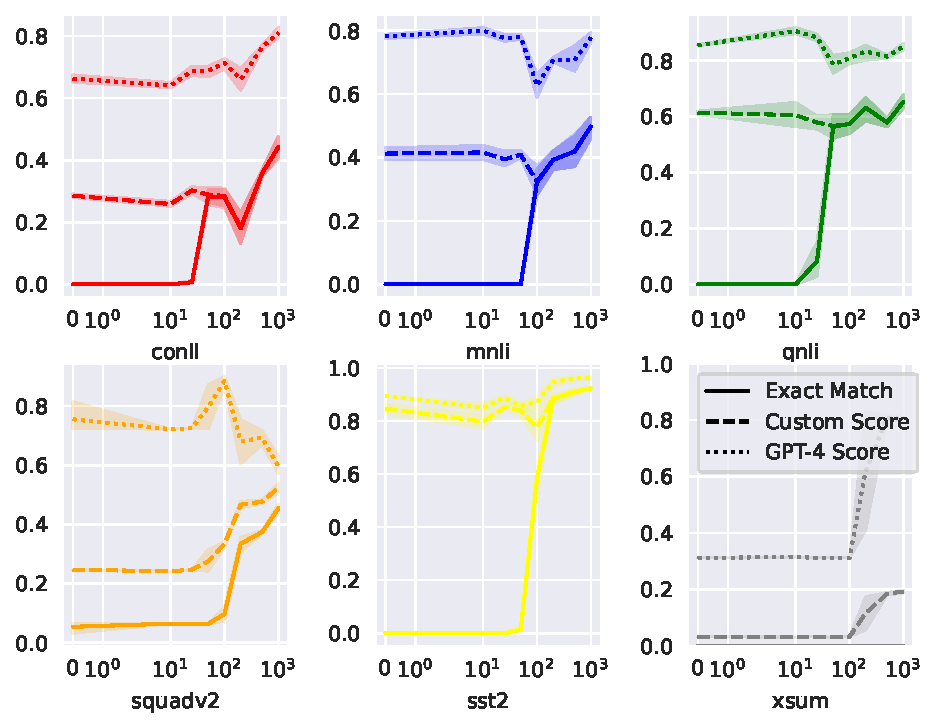
\includegraphics[width=0.5\textwidth]{images/learning_dynamics/exp1b_1.pdf}
    \caption[LLaMA performance with task samples]{LLaMA performance after incorporating $0 \leq N \leq 1000$ real task samples from respectively CONLL, MNLI, QNLI, SquadV2, SST2 and XSUM into the base training mixture}
    \label{fig:exp2}
\end{figure}


\subsubsection{Performance degradation}
\label{sec:app_perf_deg}
Full performance degradation results after 1000 samples of task-specific data are integrated within the synthetic test set are shown in \autoref{tab:perf_deg}.

\begin{table}
    \centering
    \begin{tabular}{lrrrrr}
    \toprule
     & Base & sst2 & conll & mnli & Average \\
    \midrule
    Bloom & 0.75 & 0.74 & 0.74 & 0.73 & 0.73 \\
    Falcon & 0.87 & 0.86 & 0.87 & 0.84 & 0.85 \\
    Llama & 0.84 & 0.85 & 0.86 & 0.86 & 0.86 \\
    Pythia & 0.67 & 0.66 & 0.66 & 0.66 & 0.66 \\
    \bottomrule
    \end{tabular}
    
    \caption[Alpaca test degradation]{Performance degradation on the Alpaca test set, after introducing 1000 samples of specialized data to the train set. Base denotes the reference scores, computed from the initial zero-shot performance.}
    \label{tab:perf_deg}
\end{table}



\subsection{$\mathcal{S}_2$: IFT models as Task-Specific Solvers}

\subsubsection{Experimental setup}
Models are trained in the default conditions explicited in \ref{sec:default-setup}. Starting from either a base model, or an instruction fine-tuned model, we evaluate target task performance as the model is fine-tuned solely on a varying number of target task training samples. We (i) select a target task from the real data benchmark tasks. (ii) We then sample a set of $N \in \{0, 10, 25, 50, 100, 200, 500, 1000\}$ samples from the training set, and pick 100 samples to serve as a validation split. (iii) We repeat the sampling process 4 times to mitigate variations between runs. (iv) We train one model per data mixture according to the training guidelines in \ref{sec:default-setup}. (v) We evaluate performance with all metrics listed in \ref{sec:metrics} on the target task test split.


\subsubsection{Extra models}
\label{sec:extra-datasets-exp4}
To evaluate the impact of IFT quality of the findings of the $\mathcal{S}_2$ experiment, we repeat the experiment using an "off-the-shelf" strong IFT model from the HuggingFace Hub. Notably, we select the 7B variant of \sidecite{vicuna2023} for the Llama variant, BloomZ for Bloom \sidecite{muennighoff2022crosslingual}, Falcon-Instruct for Falcon \sidecite{penedo2023refinedweb} and an IFT version of Pythia trained by \sidecite{köpf2023openassistant}. Results reported in Figure \ref{fig:exp4_old} show similar dynamics between the off-the-shelf models and the variants Instruction Fine-tuned in this work for one epoch on the Alpaca dataset \sidecite{alpaca2023}.

\begin{figure*}[ht]
    \centering
    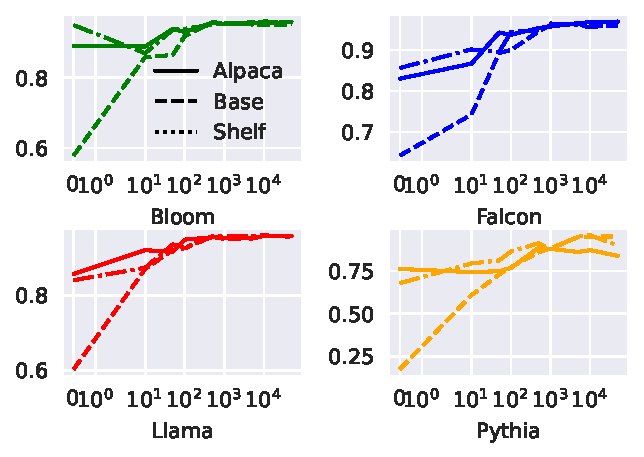
\includegraphics[width=0.8\textwidth]{images/learning_dynamics/exp4_all_old.pdf}
    \caption[GPT4 SST-2 scores]{GPT4 score on SST-2 test set after finetuning with $0 \leq N \leq 1000$  samples on a (base) LM, an "off-the-shelf" IFT model, and an IFT model fine-tuned on Alpaca.}
    \label{fig:exp4_old}
\end{figure*}

\chapter{Introduction Appendix}


\begin{figure*}
    \centering
    
\includegraphics[width = 0.95\textwidth]{images/misc/hbs_meme.jpeg}
    \caption[Library of Babel joke]{The library of Babel can actually impressively be compressed inside these two books, as goes this famous internet joke. Of course, these two books are themselves contained in the library of Babel.}
    
    % Latencies indicated in the figure are computed on the same machine \texttt{g2-standard-16} with a NVIDIA-L4 GPU, and averaged over 100 pages. Further details in \autoref{subsection:latency}.The computed score is the average of from all datasets in \textit{ViDoRe} for PDF Parser + Captioning and ColPali respectively. Further details in \autoref{section:results}.} 
    \label{fig:hbs_meme}
\end{figure*}

%----------------------------------------------------------------------------------------

\backmatter % Denotes the end of the main document content
\setchapterstyle{plain} % Output plain chapters from this point onwards

%----------------------------------------------------------------------------------------
%	BIBLIOGRAPHY
%----------------------------------------------------------------------------------------

% The bibliography needs to be compiled with biber using your LaTeX editor, or on the command line with 'biber main' from the template directory

\defbibnote{bibnote}{References are ordered in citation order.\par\bigskip} % Prepend this text to the bibliography
\printbibliography[heading=bibintoc, title=Bibliography, prenote=bibnote] % Add the bibliography heading to the ToC, set the title of the bibliography and output the bibliography note

%----------------------------------------------------------------------------------------
%	NOMENCLATURE
%----------------------------------------------------------------------------------------

% The nomenclature needs to be compiled on the command line with 'makeindex main.nlo -s nomencl.ist -o main.nls' from the template directory

% \nomenclature{$c$}{Speed of light in a vacuum inertial frame}
% \nomenclature{$h$}{Planck constant}

% \renewcommand{\nomname}{Notation} % Rename the default 'Nomenclature'
% \renewcommand{\nompreamble}{The next list describes several symbols that will be later used within the body of the document.} % Prepend this text to the nomenclature

% \printnomenclature % Output the nomenclature

% %----------------------------------------------------------------------------------------
% %	GREEK ALPHABET
% % 	Originally from https://gitlab.com/jim.hefferon/linear-algebra
% %----------------------------------------------------------------------------------------

% \vspace{1cm}

% {\usekomafont{chapter}Greek Letters with Pronunciations} \\[2ex]
% \begin{center}
% 	\newcommand{\pronounced}[1]{\hspace*{.2em}\small\textit{#1}}
% 	\begin{tabular}{l l @{\hspace*{3em}} l l}
% 		\toprule
% 		Character & Name & Character & Name \\ 
% 		\midrule
% 		$\alpha$ & alpha \pronounced{AL-fuh} & $\nu$ & nu \pronounced{NEW} \\
% 		$\beta$ & beta \pronounced{BAY-tuh} & $\xi$, $\Xi$ & xi \pronounced{KSIGH} \\ 
% 		$\gamma$, $\Gamma$ & gamma \pronounced{GAM-muh} & o & omicron \pronounced{OM-uh-CRON} \\
% 		$\delta$, $\Delta$ & delta \pronounced{DEL-tuh} & $\pi$, $\Pi$ & pi \pronounced{PIE} \\
% 		$\epsilon$ & epsilon \pronounced{EP-suh-lon} & $\rho$ & rho \pronounced{ROW} \\
% 		$\zeta$ & zeta \pronounced{ZAY-tuh} & $\sigma$, $\Sigma$ & sigma \pronounced{SIG-muh} \\
% 		$\eta$ & eta \pronounced{AY-tuh} & $\tau$ & tau \pronounced{TOW (as in cow)} \\
% 		$\theta$, $\Theta$ & theta \pronounced{THAY-tuh} & $\upsilon$, $\Upsilon$ & upsilon \pronounced{OOP-suh-LON} \\
% 		$\iota$ & iota \pronounced{eye-OH-tuh} & $\phi$, $\Phi$ & phi \pronounced{FEE, or FI (as in hi)} \\
% 		$\kappa$ & kappa \pronounced{KAP-uh} & $\chi$ & chi \pronounced{KI (as in hi)} \\
% 		$\lambda$, $\Lambda$ & lambda \pronounced{LAM-duh} & $\psi$, $\Psi$ & psi \pronounced{SIGH, or PSIGH} \\
% 		$\mu$ & mu \pronounced{MEW} & $\omega$, $\Omega$ & omega \pronounced{oh-MAY-guh} \\
% 		\bottomrule
% 	\end{tabular} \\[1.5ex]
% 	Capitals shown are the ones that differ from Roman capitals.
% \end{center}

%----------------------------------------------------------------------------------------
%	GLOSSARY
%----------------------------------------------------------------------------------------

% The glossary needs to be compiled on the command line with 'makeglossaries main' from the template directory

% \setglossarystyle{listgroup} % Set the style of the glossary (see https://en.wikibooks.org/wiki/LaTeX/Glossary for a reference)
% \printglossary[title=Special Terms, toctitle=List of Terms] % Output the glossary, 'title' is the chapter heading for the glossary, toctitle is the table of contents heading

%----------------------------------------------------------------------------------------
%	INDEX
%----------------------------------------------------------------------------------------

% The index needs to be compiled on the command line with 'makeindex main' from the template directory

% \printindex % Output the index

%----------------------------------------------------------------------------------------
%	BACK COVER
%----------------------------------------------------------------------------------------

% If you have a PDF/image file that you want to use as a back cover, uncomment the following lines

%\clearpage
%\thispagestyle{empty}
%\null%
%\clearpage
%\includepdf{cover-back.pdf}

%----------------------------------------------------------------------------------------


\end{document}
